\documentclass[twoside]{book}

% Packages required by doxygen
\usepackage{fixltx2e}
\usepackage{calc}
\usepackage{doxygen}
\usepackage[export]{adjustbox} % also loads graphicx
\usepackage{graphicx}
\usepackage[utf8]{inputenc}
\usepackage{makeidx}
\usepackage{multicol}
\usepackage{multirow}
\PassOptionsToPackage{warn}{textcomp}
\usepackage{textcomp}
\usepackage[nointegrals]{wasysym}
\usepackage[table]{xcolor}

% Font selection
\usepackage[T1]{fontenc}
\usepackage[scaled=.90]{helvet}
\usepackage{courier}
\usepackage{amssymb}
\usepackage{sectsty}
\renewcommand{\familydefault}{\sfdefault}
\allsectionsfont{%
  \fontseries{bc}\selectfont%
  \color{darkgray}%
}
\renewcommand{\DoxyLabelFont}{%
  \fontseries{bc}\selectfont%
  \color{darkgray}%
}
\newcommand{\+}{\discretionary{\mbox{\scriptsize$\hookleftarrow$}}{}{}}

% Page & text layout
\usepackage{geometry}
\geometry{%
  a4paper,%
  top=2.5cm,%
  bottom=2.5cm,%
  left=2.5cm,%
  right=2.5cm%
}
\tolerance=750
\hfuzz=15pt
\hbadness=750
\setlength{\emergencystretch}{15pt}
\setlength{\parindent}{0cm}
\setlength{\parskip}{3ex plus 2ex minus 2ex}
\makeatletter
\renewcommand{\paragraph}{%
  \@startsection{paragraph}{4}{0ex}{-1.0ex}{1.0ex}{%
    \normalfont\normalsize\bfseries\SS@parafont%
  }%
}
\renewcommand{\subparagraph}{%
  \@startsection{subparagraph}{5}{0ex}{-1.0ex}{1.0ex}{%
    \normalfont\normalsize\bfseries\SS@subparafont%
  }%
}
\makeatother

% Headers & footers
\usepackage{fancyhdr}
\pagestyle{fancyplain}
\fancyhead[LE]{\fancyplain{}{\bfseries\thepage}}
\fancyhead[CE]{\fancyplain{}{}}
\fancyhead[RE]{\fancyplain{}{\bfseries\leftmark}}
\fancyhead[LO]{\fancyplain{}{\bfseries\rightmark}}
\fancyhead[CO]{\fancyplain{}{}}
\fancyhead[RO]{\fancyplain{}{\bfseries\thepage}}
\fancyfoot[LE]{\fancyplain{}{}}
\fancyfoot[CE]{\fancyplain{}{}}
\fancyfoot[RE]{\fancyplain{}{\bfseries\scriptsize Generated by Doxygen }}
\fancyfoot[LO]{\fancyplain{}{\bfseries\scriptsize Generated by Doxygen }}
\fancyfoot[CO]{\fancyplain{}{}}
\fancyfoot[RO]{\fancyplain{}{}}
\renewcommand{\footrulewidth}{0.4pt}
\renewcommand{\chaptermark}[1]{%
  \markboth{#1}{}%
}
\renewcommand{\sectionmark}[1]{%
  \markright{\thesection\ #1}%
}

% Indices & bibliography
\usepackage{natbib}
\usepackage[titles]{tocloft}
\setcounter{tocdepth}{3}
\setcounter{secnumdepth}{5}
\makeindex

% Hyperlinks (required, but should be loaded last)
\usepackage{ifpdf}
\ifpdf
  \usepackage[pdftex,pagebackref=true]{hyperref}
\else
  \usepackage[ps2pdf,pagebackref=true]{hyperref}
\fi
\hypersetup{%
  colorlinks=true,%
  linkcolor=blue,%
  citecolor=blue,%
  unicode%
}

% Custom commands
\newcommand{\clearemptydoublepage}{%
  \newpage{\pagestyle{empty}\cleardoublepage}%
}

\usepackage{caption}
\captionsetup{labelsep=space,justification=centering,font={bf},singlelinecheck=off,skip=4pt,position=top}

%===== C O N T E N T S =====

\begin{document}

% Titlepage & ToC
\hypersetup{pageanchor=false,
             bookmarksnumbered=true,
             pdfencoding=unicode
            }
\pagenumbering{roman}
\begin{titlepage}
\vspace*{7cm}
\begin{center}%
{\Large Free\+Tacos \\[1ex]\large 1 }\\
\vspace*{1cm}
{\large Generated by Doxygen 1.8.11}\\
\end{center}
\end{titlepage}
\clearemptydoublepage
\tableofcontents
\clearemptydoublepage
\pagenumbering{arabic}
\hypersetup{pageanchor=true}

%--- Begin generated contents ---
\chapter{Hierarchical Index}
\section{Class Hierarchy}
This inheritance list is sorted roughly, but not completely, alphabetically\+:\begin{DoxyCompactList}
\item \contentsline{section}{A\+P\+P\+\_\+\+A\+T\+T\+R\+I\+B\+U\+T\+E\+\_\+\+T\+Y\+PE}{\pageref{structAPP__ATTRIBUTE__TYPE}}{}
\item \contentsline{section}{Arinc\+Module}{\pageref{classArincModule}}{}
\item \contentsline{section}{B\+L\+A\+C\+K\+B\+O\+A\+R\+D\+\_\+\+S\+T\+A\+T\+U\+S\+\_\+\+T\+Y\+PE}{\pageref{structBLACKBOARD__STATUS__TYPE}}{}
\item \contentsline{section}{B\+U\+F\+F\+E\+R\+\_\+\+S\+T\+A\+T\+U\+S\+\_\+\+T\+Y\+PE}{\pageref{structBUFFER__STATUS__TYPE}}{}
\item \contentsline{section}{Channel}{\pageref{classChannel}}{}
\item \contentsline{section}{Core\+Schedule}{\pageref{classCoreSchedule}}{}
\item C\+Stdlib\+App\+Stdio\begin{DoxyCompactList}
\item \contentsline{section}{C\+Kernel}{\pageref{classCKernel}}{}
\begin{DoxyCompactList}
\item \contentsline{section}{C\+Tacos\+Kernel}{\pageref{classCTacosKernel}}{}
\end{DoxyCompactList}
\end{DoxyCompactList}
\item \contentsline{section}{E\+R\+R\+O\+R\+\_\+\+S\+T\+A\+T\+U\+S\+\_\+\+T\+Y\+PE}{\pageref{structERROR__STATUS__TYPE}}{}
\item \contentsline{section}{Error\+Level}{\pageref{classErrorLevel}}{}
\item \contentsline{section}{E\+V\+E\+N\+T\+\_\+\+S\+T\+A\+T\+U\+S\+\_\+\+T\+Y\+PE}{\pageref{structEVENT__STATUS__TYPE}}{}
\item \contentsline{section}{I\+Process}{\pageref{classIProcess}}{}
\begin{DoxyCompactList}
\item \contentsline{section}{Prime\+Proc}{\pageref{classPrimeProc}}{}
\end{DoxyCompactList}
\item \contentsline{section}{Memory\+Region}{\pageref{classMemoryRegion}}{}
\item \contentsline{section}{Module\+Error\+Action}{\pageref{classModuleErrorAction}}{}
\item \contentsline{section}{Module\+H\+M\+Table}{\pageref{classModuleHMTable}}{}
\item \contentsline{section}{Module\+Schedule}{\pageref{classModuleSchedule}}{}
\item \contentsline{section}{Multi\+Partition\+Error\+Action}{\pageref{classMultiPartitionErrorAction}}{}
\item \contentsline{section}{Multi\+Partition\+H\+M\+Table}{\pageref{classMultiPartitionHMTable}}{}
\item \contentsline{section}{M\+U\+T\+E\+X\+\_\+\+S\+T\+A\+T\+U\+S\+\_\+\+T\+Y\+PE}{\pageref{structMUTEX__STATUS__TYPE}}{}
\item \contentsline{section}{name\+\_\+t}{\pageref{structname__t}}{}
\item \contentsline{section}{N\+A\+M\+E\+\_\+\+T\+Y\+PE}{\pageref{structNAME__TYPE}}{}
\item \contentsline{section}{Partition}{\pageref{classPartition}}{}
\item \contentsline{section}{P\+A\+R\+T\+I\+T\+I\+O\+N\+\_\+\+S\+T\+A\+T\+U\+S\+\_\+\+T\+Y\+PE}{\pageref{structPARTITION__STATUS__TYPE}}{}
\item \contentsline{section}{Partition\+Error\+Action}{\pageref{classPartitionErrorAction}}{}
\item \contentsline{section}{Partition\+H\+M\+Table}{\pageref{classPartitionHMTable}}{}
\item \contentsline{section}{Partition\+Memory}{\pageref{classPartitionMemory}}{}
\item \contentsline{section}{Partition\+Schedule}{\pageref{classPartitionSchedule}}{}
\item \contentsline{section}{Port}{\pageref{classPort}}{}
\begin{DoxyCompactList}
\item \contentsline{section}{Queuing\+Port}{\pageref{classQueuingPort}}{}
\item \contentsline{section}{Sampling\+Port}{\pageref{classSamplingPort}}{}
\end{DoxyCompactList}
\item \contentsline{section}{Port\+Mapping}{\pageref{classPortMapping}}{}
\item \contentsline{section}{Process}{\pageref{classProcess}}{}
\item \contentsline{section}{P\+R\+O\+C\+E\+S\+S\+\_\+\+A\+T\+T\+R\+I\+B\+U\+T\+E\+\_\+\+T\+Y\+PE}{\pageref{structPROCESS__ATTRIBUTE__TYPE}}{}
\item \contentsline{section}{P\+R\+O\+C\+E\+S\+S\+\_\+\+S\+T\+A\+T\+U\+S\+\_\+\+T\+Y\+PE}{\pageref{structPROCESS__STATUS__TYPE}}{}
\item \contentsline{section}{Process\+Loader}{\pageref{classProcessLoader}}{}
\item \contentsline{section}{Pseudo\+Partition}{\pageref{classPseudoPartition}}{}
\begin{DoxyCompactList}
\item \contentsline{section}{Standard\+Partition}{\pageref{classStandardPartition}}{}
\end{DoxyCompactList}
\item \contentsline{section}{Q\+U\+E\+U\+I\+N\+G\+\_\+\+P\+O\+R\+T\+\_\+\+S\+T\+A\+T\+U\+S\+\_\+\+T\+Y\+PE}{\pageref{structQUEUING__PORT__STATUS__TYPE}}{}
\item \contentsline{section}{S\+A\+M\+P\+L\+I\+N\+G\+\_\+\+P\+O\+R\+T\+\_\+\+S\+T\+A\+T\+U\+S\+\_\+\+T\+Y\+PE}{\pageref{structSAMPLING__PORT__STATUS__TYPE}}{}
\item \contentsline{section}{S\+E\+M\+A\+P\+H\+O\+R\+E\+\_\+\+S\+T\+A\+T\+U\+S\+\_\+\+T\+Y\+PE}{\pageref{structSEMAPHORE__STATUS__TYPE}}{}
\item \contentsline{section}{System\+Error}{\pageref{classSystemError}}{}
\item \contentsline{section}{System\+State\+Entry}{\pageref{classSystemStateEntry}}{}
\end{DoxyCompactList}

\chapter{Class Index}
\section{Class List}
Here are the classes, structs, unions and interfaces with brief descriptions\+:\begin{DoxyCompactList}
\item\contentsline{section}{\hyperlink{structAPP__ATTRIBUTE__TYPE}{A\+P\+P\+\_\+\+A\+T\+T\+R\+I\+B\+U\+T\+E\+\_\+\+T\+Y\+PE} }{\pageref{structAPP__ATTRIBUTE__TYPE}}{}
\item\contentsline{section}{\hyperlink{classArincModule}{Arinc\+Module} }{\pageref{classArincModule}}{}
\item\contentsline{section}{\hyperlink{structBLACKBOARD__STATUS__TYPE}{B\+L\+A\+C\+K\+B\+O\+A\+R\+D\+\_\+\+S\+T\+A\+T\+U\+S\+\_\+\+T\+Y\+PE} }{\pageref{structBLACKBOARD__STATUS__TYPE}}{}
\item\contentsline{section}{\hyperlink{structBUFFER__STATUS__TYPE}{B\+U\+F\+F\+E\+R\+\_\+\+S\+T\+A\+T\+U\+S\+\_\+\+T\+Y\+PE} }{\pageref{structBUFFER__STATUS__TYPE}}{}
\item\contentsline{section}{\hyperlink{classChannel}{Channel} }{\pageref{classChannel}}{}
\item\contentsline{section}{\hyperlink{classCKernel}{C\+Kernel} }{\pageref{classCKernel}}{}
\item\contentsline{section}{\hyperlink{classCoreSchedule}{Core\+Schedule} }{\pageref{classCoreSchedule}}{}
\item\contentsline{section}{\hyperlink{classCTacosKernel}{C\+Tacos\+Kernel} }{\pageref{classCTacosKernel}}{}
\item\contentsline{section}{\hyperlink{structERROR__STATUS__TYPE}{E\+R\+R\+O\+R\+\_\+\+S\+T\+A\+T\+U\+S\+\_\+\+T\+Y\+PE} }{\pageref{structERROR__STATUS__TYPE}}{}
\item\contentsline{section}{\hyperlink{classErrorLevel}{Error\+Level} }{\pageref{classErrorLevel}}{}
\item\contentsline{section}{\hyperlink{structEVENT__STATUS__TYPE}{E\+V\+E\+N\+T\+\_\+\+S\+T\+A\+T\+U\+S\+\_\+\+T\+Y\+PE} }{\pageref{structEVENT__STATUS__TYPE}}{}
\item\contentsline{section}{\hyperlink{classIProcess}{I\+Process} }{\pageref{classIProcess}}{}
\item\contentsline{section}{\hyperlink{classMemoryRegion}{Memory\+Region} }{\pageref{classMemoryRegion}}{}
\item\contentsline{section}{\hyperlink{classModuleErrorAction}{Module\+Error\+Action} }{\pageref{classModuleErrorAction}}{}
\item\contentsline{section}{\hyperlink{classModuleHMTable}{Module\+H\+M\+Table} }{\pageref{classModuleHMTable}}{}
\item\contentsline{section}{\hyperlink{classModuleSchedule}{Module\+Schedule} }{\pageref{classModuleSchedule}}{}
\item\contentsline{section}{\hyperlink{classMultiPartitionErrorAction}{Multi\+Partition\+Error\+Action} }{\pageref{classMultiPartitionErrorAction}}{}
\item\contentsline{section}{\hyperlink{classMultiPartitionHMTable}{Multi\+Partition\+H\+M\+Table} }{\pageref{classMultiPartitionHMTable}}{}
\item\contentsline{section}{\hyperlink{structMUTEX__STATUS__TYPE}{M\+U\+T\+E\+X\+\_\+\+S\+T\+A\+T\+U\+S\+\_\+\+T\+Y\+PE} }{\pageref{structMUTEX__STATUS__TYPE}}{}
\item\contentsline{section}{\hyperlink{structname__t}{name\+\_\+t} }{\pageref{structname__t}}{}
\item\contentsline{section}{\hyperlink{structNAME__TYPE}{N\+A\+M\+E\+\_\+\+T\+Y\+PE} }{\pageref{structNAME__TYPE}}{}
\item\contentsline{section}{\hyperlink{classPartition}{Partition} }{\pageref{classPartition}}{}
\item\contentsline{section}{\hyperlink{structPARTITION__STATUS__TYPE}{P\+A\+R\+T\+I\+T\+I\+O\+N\+\_\+\+S\+T\+A\+T\+U\+S\+\_\+\+T\+Y\+PE} }{\pageref{structPARTITION__STATUS__TYPE}}{}
\item\contentsline{section}{\hyperlink{classPartitionErrorAction}{Partition\+Error\+Action} }{\pageref{classPartitionErrorAction}}{}
\item\contentsline{section}{\hyperlink{classPartitionHMTable}{Partition\+H\+M\+Table} }{\pageref{classPartitionHMTable}}{}
\item\contentsline{section}{\hyperlink{classPartitionMemory}{Partition\+Memory} }{\pageref{classPartitionMemory}}{}
\item\contentsline{section}{\hyperlink{classPartitionSchedule}{Partition\+Schedule} }{\pageref{classPartitionSchedule}}{}
\item\contentsline{section}{\hyperlink{classPort}{Port} }{\pageref{classPort}}{}
\item\contentsline{section}{\hyperlink{classPortMapping}{Port\+Mapping} }{\pageref{classPortMapping}}{}
\item\contentsline{section}{\hyperlink{classPrimeProc}{Prime\+Proc} }{\pageref{classPrimeProc}}{}
\item\contentsline{section}{\hyperlink{classProcess}{Process} }{\pageref{classProcess}}{}
\item\contentsline{section}{\hyperlink{structPROCESS__ATTRIBUTE__TYPE}{P\+R\+O\+C\+E\+S\+S\+\_\+\+A\+T\+T\+R\+I\+B\+U\+T\+E\+\_\+\+T\+Y\+PE} }{\pageref{structPROCESS__ATTRIBUTE__TYPE}}{}
\item\contentsline{section}{\hyperlink{structPROCESS__STATUS__TYPE}{P\+R\+O\+C\+E\+S\+S\+\_\+\+S\+T\+A\+T\+U\+S\+\_\+\+T\+Y\+PE} }{\pageref{structPROCESS__STATUS__TYPE}}{}
\item\contentsline{section}{\hyperlink{classProcessLoader}{Process\+Loader} }{\pageref{classProcessLoader}}{}
\item\contentsline{section}{\hyperlink{classPseudoPartition}{Pseudo\+Partition} }{\pageref{classPseudoPartition}}{}
\item\contentsline{section}{\hyperlink{structQUEUING__PORT__STATUS__TYPE}{Q\+U\+E\+U\+I\+N\+G\+\_\+\+P\+O\+R\+T\+\_\+\+S\+T\+A\+T\+U\+S\+\_\+\+T\+Y\+PE} }{\pageref{structQUEUING__PORT__STATUS__TYPE}}{}
\item\contentsline{section}{\hyperlink{classQueuingPort}{Queuing\+Port} }{\pageref{classQueuingPort}}{}
\item\contentsline{section}{\hyperlink{structSAMPLING__PORT__STATUS__TYPE}{S\+A\+M\+P\+L\+I\+N\+G\+\_\+\+P\+O\+R\+T\+\_\+\+S\+T\+A\+T\+U\+S\+\_\+\+T\+Y\+PE} }{\pageref{structSAMPLING__PORT__STATUS__TYPE}}{}
\item\contentsline{section}{\hyperlink{classSamplingPort}{Sampling\+Port} }{\pageref{classSamplingPort}}{}
\item\contentsline{section}{\hyperlink{structSEMAPHORE__STATUS__TYPE}{S\+E\+M\+A\+P\+H\+O\+R\+E\+\_\+\+S\+T\+A\+T\+U\+S\+\_\+\+T\+Y\+PE} }{\pageref{structSEMAPHORE__STATUS__TYPE}}{}
\item\contentsline{section}{\hyperlink{classStandardPartition}{Standard\+Partition} }{\pageref{classStandardPartition}}{}
\item\contentsline{section}{\hyperlink{classSystemError}{System\+Error} }{\pageref{classSystemError}}{}
\item\contentsline{section}{\hyperlink{classSystemStateEntry}{System\+State\+Entry} }{\pageref{classSystemStateEntry}}{}
\end{DoxyCompactList}

\chapter{File Index}
\section{File List}
Here is a list of all files with brief descriptions\+:\begin{DoxyCompactList}
\item\contentsline{section}{sample/01-\/gpiosimple/\hyperlink{kernel_8cpp}{kernel.\+cpp} }{\pageref{kernel_8cpp}}{}
\item\contentsline{section}{sample/01-\/gpiosimple/\hyperlink{kernel_8h}{kernel.\+h} }{\pageref{kernel_8h}}{}
\item\contentsline{section}{sample/01-\/gpiosimple/\hyperlink{sample_201-gpiosimple_2main_8cpp}{main.\+cpp} }{\pageref{sample_201-gpiosimple_2main_8cpp}}{}
\item\contentsline{section}{src/\hyperlink{src_2main_8cpp}{main.\+cpp} }{\pageref{src_2main_8cpp}}{}
\item\contentsline{section}{src/apps/\hyperlink{primeproc_8cpp}{primeproc.\+cpp} }{\pageref{primeproc_8cpp}}{}
\item\contentsline{section}{src/apps/\hyperlink{primeproc_8h}{primeproc.\+h} }{\pageref{primeproc_8h}}{}
\item\contentsline{section}{src/kernel/\hyperlink{kernel_2arinc__module_8cpp}{arinc\+\_\+module.\+cpp} }{\pageref{kernel_2arinc__module_8cpp}}{}
\item\contentsline{section}{src/kernel/\hyperlink{config_8cpp}{config.\+cpp} }{\pageref{config_8cpp}}{}
\item\contentsline{section}{src/kernel/\hyperlink{core__schedule_8cpp}{core\+\_\+schedule.\+cpp} }{\pageref{core__schedule_8cpp}}{}
\item\contentsline{section}{src/kernel/\hyperlink{src_2kernel_2main_8cpp}{main.\+cpp} }{\pageref{src_2kernel_2main_8cpp}}{}
\item\contentsline{section}{src/kernel/arch/rasp4/\hyperlink{arch_8cpp}{arch.\+cpp} }{\pageref{arch_8cpp}}{}
\item\contentsline{section}{src/kernel/core/\hyperlink{boot_8cpp}{boot.\+cpp} }{\pageref{boot_8cpp}}{}
\item\contentsline{section}{src/kernel/core/\hyperlink{processloader_8cpp}{processloader.\+cpp} }{\pageref{processloader_8cpp}}{}
\item\contentsline{section}{src/kernel/core/\hyperlink{processloader_8h}{processloader.\+h} }{\pageref{processloader_8h}}{}
\item\contentsline{section}{src/kernel/core/\hyperlink{tacoskernel_8cpp}{tacoskernel.\+cpp} }{\pageref{tacoskernel_8cpp}}{}
\item\contentsline{section}{src/kernel/core/\hyperlink{tacoskernel_8h}{tacoskernel.\+h} }{\pageref{tacoskernel_8h}}{}
\item\contentsline{section}{src/kernel/core/process/\hyperlink{processinterface_8cpp}{processinterface.\+cpp} }{\pageref{processinterface_8cpp}}{}
\item\contentsline{section}{src/kernel/core/process/\hyperlink{processinterface_8h}{processinterface.\+h} }{\pageref{processinterface_8h}}{}
\item\contentsline{section}{src/kernel/include/\hyperlink{arch_8h}{arch.\+h} }{\pageref{arch_8h}}{}
\item\contentsline{section}{src/kernel/include/\hyperlink{errcode_8h}{errcode.\+h} }{\pageref{errcode_8h}}{}
\item\contentsline{section}{src/kernel/include/core/\hyperlink{boot_8h}{boot.\+h} }{\pageref{boot_8h}}{}
\item\contentsline{section}{src/libuser/apex/\hyperlink{apex__blackboard_8h}{apex\+\_\+blackboard.\+h} }{\pageref{apex__blackboard_8h}}{}
\item\contentsline{section}{src/libuser/apex/\hyperlink{apex__buffer_8h}{apex\+\_\+buffer.\+h} }{\pageref{apex__buffer_8h}}{}
\item\contentsline{section}{src/libuser/apex/\hyperlink{apex__error_8h}{apex\+\_\+error.\+h} }{\pageref{apex__error_8h}}{}
\item\contentsline{section}{src/libuser/apex/\hyperlink{apex__event_8h}{apex\+\_\+event.\+h} }{\pageref{apex__event_8h}}{}
\item\contentsline{section}{src/libuser/apex/\hyperlink{apex__mutex_8h}{apex\+\_\+mutex.\+h} }{\pageref{apex__mutex_8h}}{}
\item\contentsline{section}{src/libuser/apex/\hyperlink{apex__partition_8h}{apex\+\_\+partition.\+h} }{\pageref{apex__partition_8h}}{}
\item\contentsline{section}{src/libuser/apex/\hyperlink{apex__process_8h}{apex\+\_\+process.\+h} }{\pageref{apex__process_8h}}{}
\item\contentsline{section}{src/libuser/apex/\hyperlink{apex__queuing__port_8h}{apex\+\_\+queuing\+\_\+port.\+h} }{\pageref{apex__queuing__port_8h}}{}
\item\contentsline{section}{src/libuser/apex/\hyperlink{apex__sampling__port_8h}{apex\+\_\+sampling\+\_\+port.\+h} }{\pageref{apex__sampling__port_8h}}{}
\item\contentsline{section}{src/libuser/apex/\hyperlink{apex__semaphore_8h}{apex\+\_\+semaphore.\+h} }{\pageref{apex__semaphore_8h}}{}
\item\contentsline{section}{src/libuser/apex/\hyperlink{apex__time_8h}{apex\+\_\+time.\+h} }{\pageref{apex__time_8h}}{}
\item\contentsline{section}{src/libuser/apex/\hyperlink{apex__types_8h}{apex\+\_\+types.\+h} }{\pageref{apex__types_8h}}{}
\item\contentsline{section}{src/types/include/\hyperlink{arinc__module_8hpp}{arinc\+\_\+module.\+hpp} }{\pageref{arinc__module_8hpp}}{}
\item\contentsline{section}{src/types/include/\hyperlink{channel_8hpp}{channel.\+hpp} }{\pageref{channel_8hpp}}{}
\item\contentsline{section}{src/types/include/\hyperlink{core__schedule_8hpp}{core\+\_\+schedule.\+hpp} }{\pageref{core__schedule_8hpp}}{}
\item\contentsline{section}{src/types/include/\hyperlink{error__level_8hpp}{error\+\_\+level.\+hpp} }{\pageref{error__level_8hpp}}{}
\item\contentsline{section}{src/types/include/\hyperlink{general__types_8hpp}{general\+\_\+types.\+hpp} }{\pageref{general__types_8hpp}}{}
\item\contentsline{section}{src/types/include/\hyperlink{memory__requirements_8hpp}{memory\+\_\+requirements.\+hpp} }{\pageref{memory__requirements_8hpp}}{}
\item\contentsline{section}{src/types/include/\hyperlink{module__error__action_8hpp}{module\+\_\+error\+\_\+action.\+hpp} }{\pageref{module__error__action_8hpp}}{}
\item\contentsline{section}{src/types/include/\hyperlink{module__hm__table_8hpp}{module\+\_\+hm\+\_\+table.\+hpp} }{\pageref{module__hm__table_8hpp}}{}
\item\contentsline{section}{src/types/include/\hyperlink{module__schedule_8hpp}{module\+\_\+schedule.\+hpp} }{\pageref{module__schedule_8hpp}}{}
\item\contentsline{section}{src/types/include/\hyperlink{multipartition__error__action_8hpp}{multipartition\+\_\+error\+\_\+action.\+hpp} }{\pageref{multipartition__error__action_8hpp}}{}
\item\contentsline{section}{src/types/include/\hyperlink{multipartition__hm__table_8hpp}{multipartition\+\_\+hm\+\_\+table.\+hpp} }{\pageref{multipartition__hm__table_8hpp}}{}
\item\contentsline{section}{src/types/include/\hyperlink{partition_8hpp}{partition.\+hpp} }{\pageref{partition_8hpp}}{}
\item\contentsline{section}{src/types/include/\hyperlink{partition__error__action_8hpp}{partition\+\_\+error\+\_\+action.\+hpp} }{\pageref{partition__error__action_8hpp}}{}
\item\contentsline{section}{src/types/include/\hyperlink{partition__hm__table_8hpp}{partition\+\_\+hm\+\_\+table.\+hpp} }{\pageref{partition__hm__table_8hpp}}{}
\item\contentsline{section}{src/types/include/\hyperlink{partition__memory_8hpp}{partition\+\_\+memory.\+hpp} }{\pageref{partition__memory_8hpp}}{}
\item\contentsline{section}{src/types/include/\hyperlink{partition__schedule_8hpp}{partition\+\_\+schedule.\+hpp} }{\pageref{partition__schedule_8hpp}}{}
\item\contentsline{section}{src/types/include/\hyperlink{port_8hpp}{port.\+hpp} }{\pageref{port_8hpp}}{}
\item\contentsline{section}{src/types/include/\hyperlink{port__mapping_8hpp}{port\+\_\+mapping.\+hpp} }{\pageref{port__mapping_8hpp}}{}
\item\contentsline{section}{src/types/include/\hyperlink{process_8hpp}{process.\+hpp} }{\pageref{process_8hpp}}{}
\item\contentsline{section}{src/types/include/\hyperlink{pseudo__partition_8hpp}{pseudo\+\_\+partition.\+hpp} }{\pageref{pseudo__partition_8hpp}}{}
\item\contentsline{section}{src/types/include/\hyperlink{queuing__port_8hpp}{queuing\+\_\+port.\+hpp} }{\pageref{queuing__port_8hpp}}{}
\item\contentsline{section}{src/types/include/\hyperlink{sampling__port_8hpp}{sampling\+\_\+port.\+hpp} }{\pageref{sampling__port_8hpp}}{}
\item\contentsline{section}{src/types/include/\hyperlink{standard__partition_8hpp}{standard\+\_\+partition.\+hpp} }{\pageref{standard__partition_8hpp}}{}
\item\contentsline{section}{src/types/include/\hyperlink{system__error_8hpp}{system\+\_\+error.\+hpp} }{\pageref{system__error_8hpp}}{}
\item\contentsline{section}{src/types/include/\hyperlink{system__state__entry_8hpp}{system\+\_\+state\+\_\+entry.\+hpp} }{\pageref{system__state__entry_8hpp}}{}
\item\contentsline{section}{src/types/src/\hyperlink{types_2src_2arinc__module_8cpp}{arinc\+\_\+module.\+cpp} }{\pageref{types_2src_2arinc__module_8cpp}}{}
\item\contentsline{section}{src/types/src/\hyperlink{channel_8cpp}{channel.\+cpp} }{\pageref{channel_8cpp}}{}
\item\contentsline{section}{src/types/src/\hyperlink{error__level_8cpp}{error\+\_\+level.\+cpp} }{\pageref{error__level_8cpp}}{}
\item\contentsline{section}{src/types/src/\hyperlink{memory__requirements_8cpp}{memory\+\_\+requirements.\+cpp} }{\pageref{memory__requirements_8cpp}}{}
\item\contentsline{section}{src/types/src/\hyperlink{module__error__action_8cpp}{module\+\_\+error\+\_\+action.\+cpp} }{\pageref{module__error__action_8cpp}}{}
\item\contentsline{section}{src/types/src/\hyperlink{module__hm__table_8cpp}{module\+\_\+hm\+\_\+table.\+cpp} }{\pageref{module__hm__table_8cpp}}{}
\item\contentsline{section}{src/types/src/\hyperlink{module__schedule_8cpp}{module\+\_\+schedule.\+cpp} }{\pageref{module__schedule_8cpp}}{}
\item\contentsline{section}{src/types/src/\hyperlink{multipartition__error__action_8cpp}{multipartition\+\_\+error\+\_\+action.\+cpp} }{\pageref{multipartition__error__action_8cpp}}{}
\item\contentsline{section}{src/types/src/\hyperlink{multipartition__hm__table_8cpp}{multipartition\+\_\+hm\+\_\+table.\+cpp} }{\pageref{multipartition__hm__table_8cpp}}{}
\item\contentsline{section}{src/types/src/\hyperlink{partition_8cpp}{partition.\+cpp} }{\pageref{partition_8cpp}}{}
\item\contentsline{section}{src/types/src/\hyperlink{partition__hm__table_8cpp}{partition\+\_\+hm\+\_\+table.\+cpp} }{\pageref{partition__hm__table_8cpp}}{}
\item\contentsline{section}{src/types/src/\hyperlink{partition__memory_8cpp}{partition\+\_\+memory.\+cpp} }{\pageref{partition__memory_8cpp}}{}
\item\contentsline{section}{src/types/src/\hyperlink{partition__schedule_8cpp}{partition\+\_\+schedule.\+cpp} }{\pageref{partition__schedule_8cpp}}{}
\item\contentsline{section}{src/types/src/\hyperlink{patititon__error__action_8cpp}{patititon\+\_\+error\+\_\+action.\+cpp} }{\pageref{patititon__error__action_8cpp}}{}
\item\contentsline{section}{src/types/src/\hyperlink{port_8cpp}{port.\+cpp} }{\pageref{port_8cpp}}{}
\item\contentsline{section}{src/types/src/\hyperlink{port__mapping_8cpp}{port\+\_\+mapping.\+cpp} }{\pageref{port__mapping_8cpp}}{}
\item\contentsline{section}{src/types/src/\hyperlink{process_8cpp}{process.\+cpp} }{\pageref{process_8cpp}}{}
\item\contentsline{section}{src/types/src/\hyperlink{pseudo__partition_8cpp}{pseudo\+\_\+partition.\+cpp} }{\pageref{pseudo__partition_8cpp}}{}
\item\contentsline{section}{src/types/src/\hyperlink{queuing__port_8cpp}{queuing\+\_\+port.\+cpp} }{\pageref{queuing__port_8cpp}}{}
\item\contentsline{section}{src/types/src/\hyperlink{sampling__port_8cpp}{sampling\+\_\+port.\+cpp} }{\pageref{sampling__port_8cpp}}{}
\item\contentsline{section}{src/types/src/\hyperlink{standard__partition_8cpp}{standard\+\_\+partition.\+cpp} }{\pageref{standard__partition_8cpp}}{}
\item\contentsline{section}{src/types/src/\hyperlink{system__error_8cpp}{system\+\_\+error.\+cpp} }{\pageref{system__error_8cpp}}{}
\item\contentsline{section}{src/types/src/\hyperlink{system__state__entry_8cpp}{system\+\_\+state\+\_\+entry.\+cpp} }{\pageref{system__state__entry_8cpp}}{}
\end{DoxyCompactList}

\chapter{Class Documentation}
\hypertarget{structAPP__ATTRIBUTE__TYPE}{}\section{A\+P\+P\+\_\+\+A\+T\+T\+R\+I\+B\+U\+T\+E\+\_\+\+T\+Y\+PE Struct Reference}
\label{structAPP__ATTRIBUTE__TYPE}\index{A\+P\+P\+\_\+\+A\+T\+T\+R\+I\+B\+U\+T\+E\+\_\+\+T\+Y\+PE@{A\+P\+P\+\_\+\+A\+T\+T\+R\+I\+B\+U\+T\+E\+\_\+\+T\+Y\+PE}}


{\ttfamily \#include $<$apex\+\_\+process.\+h$>$}



Collaboration diagram for A\+P\+P\+\_\+\+A\+T\+T\+R\+I\+B\+U\+T\+E\+\_\+\+T\+Y\+PE\+:
\nopagebreak
\begin{figure}[H]
\begin{center}
\leavevmode
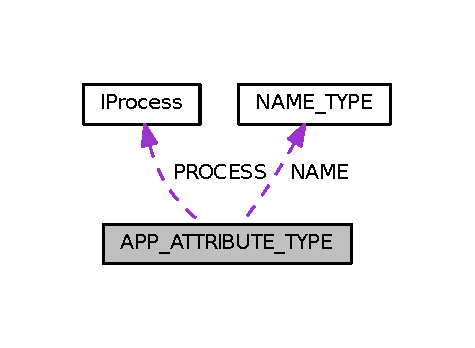
\includegraphics[width=228pt]{structAPP__ATTRIBUTE__TYPE__coll__graph}
\end{center}
\end{figure}
\subsection*{Public Attributes}
\begin{DoxyCompactItemize}
\item 
\hyperlink{apex__types_8h_a78cd52c2621ddf2eda68fcd4bedbc1a7}{S\+Y\+S\+T\+E\+M\+\_\+\+T\+I\+M\+E\+\_\+\+T\+Y\+PE} \hyperlink{structAPP__ATTRIBUTE__TYPE_a47b84ff0600db67ef9aa39d83a331955}{P\+E\+R\+I\+OD}
\item 
\hyperlink{apex__types_8h_a78cd52c2621ddf2eda68fcd4bedbc1a7}{S\+Y\+S\+T\+E\+M\+\_\+\+T\+I\+M\+E\+\_\+\+T\+Y\+PE} \hyperlink{structAPP__ATTRIBUTE__TYPE_ab25da03c2b34897d67cafff51e29a245}{T\+I\+M\+E\+\_\+\+C\+A\+P\+A\+C\+I\+TY}
\item 
\hyperlink{classIProcess}{I\+Process} \& \hyperlink{structAPP__ATTRIBUTE__TYPE_a058460c2ea56888e4475bc2459109b0f}{P\+R\+O\+C\+E\+SS}
\item 
\hyperlink{apex__process_8h_a88a1e60035e9edf9ff430765543659b2}{S\+T\+A\+C\+K\+\_\+\+S\+I\+Z\+E\+\_\+\+T\+Y\+PE} \hyperlink{structAPP__ATTRIBUTE__TYPE_a7a3ca2ad2e76aa9643e5338934326ee2}{S\+T\+A\+C\+K\+\_\+\+S\+I\+ZE}
\item 
\hyperlink{apex__process_8h_a2185443fe5bfda31ff9cce2071f1b18c}{P\+R\+I\+O\+R\+I\+T\+Y\+\_\+\+T\+Y\+PE} \hyperlink{structAPP__ATTRIBUTE__TYPE_a6bdb572015a03ef421f829030f6c7f9b}{B\+A\+S\+E\+\_\+\+P\+R\+I\+O\+R\+I\+TY}
\item 
\hyperlink{apex__process_8h_a930759cec98a9372ee6b92c4c20223fe}{D\+E\+A\+D\+L\+I\+N\+E\+\_\+\+T\+Y\+PE} \hyperlink{structAPP__ATTRIBUTE__TYPE_ae5e63ade4f66e5781611efa15681255d}{D\+E\+A\+D\+L\+I\+NE}
\item 
\hyperlink{apex__process_8h_a50887e4c49611fad19176906f38db47c}{P\+R\+O\+C\+E\+S\+S\+\_\+\+N\+A\+M\+E\+\_\+\+T\+Y\+PE} \hyperlink{structAPP__ATTRIBUTE__TYPE_afdedeaea6179501d4e5d87843b5c88a2}{N\+A\+ME}
\end{DoxyCompactItemize}


\subsection{Member Data Documentation}
\index{A\+P\+P\+\_\+\+A\+T\+T\+R\+I\+B\+U\+T\+E\+\_\+\+T\+Y\+PE@{A\+P\+P\+\_\+\+A\+T\+T\+R\+I\+B\+U\+T\+E\+\_\+\+T\+Y\+PE}!B\+A\+S\+E\+\_\+\+P\+R\+I\+O\+R\+I\+TY@{B\+A\+S\+E\+\_\+\+P\+R\+I\+O\+R\+I\+TY}}
\index{B\+A\+S\+E\+\_\+\+P\+R\+I\+O\+R\+I\+TY@{B\+A\+S\+E\+\_\+\+P\+R\+I\+O\+R\+I\+TY}!A\+P\+P\+\_\+\+A\+T\+T\+R\+I\+B\+U\+T\+E\+\_\+\+T\+Y\+PE@{A\+P\+P\+\_\+\+A\+T\+T\+R\+I\+B\+U\+T\+E\+\_\+\+T\+Y\+PE}}
\subsubsection[{\texorpdfstring{B\+A\+S\+E\+\_\+\+P\+R\+I\+O\+R\+I\+TY}{BASE_PRIORITY}}]{\setlength{\rightskip}{0pt plus 5cm}{\bf P\+R\+I\+O\+R\+I\+T\+Y\+\_\+\+T\+Y\+PE} A\+P\+P\+\_\+\+A\+T\+T\+R\+I\+B\+U\+T\+E\+\_\+\+T\+Y\+P\+E\+::\+B\+A\+S\+E\+\_\+\+P\+R\+I\+O\+R\+I\+TY}\hypertarget{structAPP__ATTRIBUTE__TYPE_a6bdb572015a03ef421f829030f6c7f9b}{}\label{structAPP__ATTRIBUTE__TYPE_a6bdb572015a03ef421f829030f6c7f9b}
\index{A\+P\+P\+\_\+\+A\+T\+T\+R\+I\+B\+U\+T\+E\+\_\+\+T\+Y\+PE@{A\+P\+P\+\_\+\+A\+T\+T\+R\+I\+B\+U\+T\+E\+\_\+\+T\+Y\+PE}!D\+E\+A\+D\+L\+I\+NE@{D\+E\+A\+D\+L\+I\+NE}}
\index{D\+E\+A\+D\+L\+I\+NE@{D\+E\+A\+D\+L\+I\+NE}!A\+P\+P\+\_\+\+A\+T\+T\+R\+I\+B\+U\+T\+E\+\_\+\+T\+Y\+PE@{A\+P\+P\+\_\+\+A\+T\+T\+R\+I\+B\+U\+T\+E\+\_\+\+T\+Y\+PE}}
\subsubsection[{\texorpdfstring{D\+E\+A\+D\+L\+I\+NE}{DEADLINE}}]{\setlength{\rightskip}{0pt plus 5cm}{\bf D\+E\+A\+D\+L\+I\+N\+E\+\_\+\+T\+Y\+PE} A\+P\+P\+\_\+\+A\+T\+T\+R\+I\+B\+U\+T\+E\+\_\+\+T\+Y\+P\+E\+::\+D\+E\+A\+D\+L\+I\+NE}\hypertarget{structAPP__ATTRIBUTE__TYPE_ae5e63ade4f66e5781611efa15681255d}{}\label{structAPP__ATTRIBUTE__TYPE_ae5e63ade4f66e5781611efa15681255d}
\index{A\+P\+P\+\_\+\+A\+T\+T\+R\+I\+B\+U\+T\+E\+\_\+\+T\+Y\+PE@{A\+P\+P\+\_\+\+A\+T\+T\+R\+I\+B\+U\+T\+E\+\_\+\+T\+Y\+PE}!N\+A\+ME@{N\+A\+ME}}
\index{N\+A\+ME@{N\+A\+ME}!A\+P\+P\+\_\+\+A\+T\+T\+R\+I\+B\+U\+T\+E\+\_\+\+T\+Y\+PE@{A\+P\+P\+\_\+\+A\+T\+T\+R\+I\+B\+U\+T\+E\+\_\+\+T\+Y\+PE}}
\subsubsection[{\texorpdfstring{N\+A\+ME}{NAME}}]{\setlength{\rightskip}{0pt plus 5cm}{\bf P\+R\+O\+C\+E\+S\+S\+\_\+\+N\+A\+M\+E\+\_\+\+T\+Y\+PE} A\+P\+P\+\_\+\+A\+T\+T\+R\+I\+B\+U\+T\+E\+\_\+\+T\+Y\+P\+E\+::\+N\+A\+ME}\hypertarget{structAPP__ATTRIBUTE__TYPE_afdedeaea6179501d4e5d87843b5c88a2}{}\label{structAPP__ATTRIBUTE__TYPE_afdedeaea6179501d4e5d87843b5c88a2}
\index{A\+P\+P\+\_\+\+A\+T\+T\+R\+I\+B\+U\+T\+E\+\_\+\+T\+Y\+PE@{A\+P\+P\+\_\+\+A\+T\+T\+R\+I\+B\+U\+T\+E\+\_\+\+T\+Y\+PE}!P\+E\+R\+I\+OD@{P\+E\+R\+I\+OD}}
\index{P\+E\+R\+I\+OD@{P\+E\+R\+I\+OD}!A\+P\+P\+\_\+\+A\+T\+T\+R\+I\+B\+U\+T\+E\+\_\+\+T\+Y\+PE@{A\+P\+P\+\_\+\+A\+T\+T\+R\+I\+B\+U\+T\+E\+\_\+\+T\+Y\+PE}}
\subsubsection[{\texorpdfstring{P\+E\+R\+I\+OD}{PERIOD}}]{\setlength{\rightskip}{0pt plus 5cm}{\bf S\+Y\+S\+T\+E\+M\+\_\+\+T\+I\+M\+E\+\_\+\+T\+Y\+PE} A\+P\+P\+\_\+\+A\+T\+T\+R\+I\+B\+U\+T\+E\+\_\+\+T\+Y\+P\+E\+::\+P\+E\+R\+I\+OD}\hypertarget{structAPP__ATTRIBUTE__TYPE_a47b84ff0600db67ef9aa39d83a331955}{}\label{structAPP__ATTRIBUTE__TYPE_a47b84ff0600db67ef9aa39d83a331955}
\index{A\+P\+P\+\_\+\+A\+T\+T\+R\+I\+B\+U\+T\+E\+\_\+\+T\+Y\+PE@{A\+P\+P\+\_\+\+A\+T\+T\+R\+I\+B\+U\+T\+E\+\_\+\+T\+Y\+PE}!P\+R\+O\+C\+E\+SS@{P\+R\+O\+C\+E\+SS}}
\index{P\+R\+O\+C\+E\+SS@{P\+R\+O\+C\+E\+SS}!A\+P\+P\+\_\+\+A\+T\+T\+R\+I\+B\+U\+T\+E\+\_\+\+T\+Y\+PE@{A\+P\+P\+\_\+\+A\+T\+T\+R\+I\+B\+U\+T\+E\+\_\+\+T\+Y\+PE}}
\subsubsection[{\texorpdfstring{P\+R\+O\+C\+E\+SS}{PROCESS}}]{\setlength{\rightskip}{0pt plus 5cm}{\bf I\+Process}\& A\+P\+P\+\_\+\+A\+T\+T\+R\+I\+B\+U\+T\+E\+\_\+\+T\+Y\+P\+E\+::\+P\+R\+O\+C\+E\+SS}\hypertarget{structAPP__ATTRIBUTE__TYPE_a058460c2ea56888e4475bc2459109b0f}{}\label{structAPP__ATTRIBUTE__TYPE_a058460c2ea56888e4475bc2459109b0f}
\index{A\+P\+P\+\_\+\+A\+T\+T\+R\+I\+B\+U\+T\+E\+\_\+\+T\+Y\+PE@{A\+P\+P\+\_\+\+A\+T\+T\+R\+I\+B\+U\+T\+E\+\_\+\+T\+Y\+PE}!S\+T\+A\+C\+K\+\_\+\+S\+I\+ZE@{S\+T\+A\+C\+K\+\_\+\+S\+I\+ZE}}
\index{S\+T\+A\+C\+K\+\_\+\+S\+I\+ZE@{S\+T\+A\+C\+K\+\_\+\+S\+I\+ZE}!A\+P\+P\+\_\+\+A\+T\+T\+R\+I\+B\+U\+T\+E\+\_\+\+T\+Y\+PE@{A\+P\+P\+\_\+\+A\+T\+T\+R\+I\+B\+U\+T\+E\+\_\+\+T\+Y\+PE}}
\subsubsection[{\texorpdfstring{S\+T\+A\+C\+K\+\_\+\+S\+I\+ZE}{STACK_SIZE}}]{\setlength{\rightskip}{0pt plus 5cm}{\bf S\+T\+A\+C\+K\+\_\+\+S\+I\+Z\+E\+\_\+\+T\+Y\+PE} A\+P\+P\+\_\+\+A\+T\+T\+R\+I\+B\+U\+T\+E\+\_\+\+T\+Y\+P\+E\+::\+S\+T\+A\+C\+K\+\_\+\+S\+I\+ZE}\hypertarget{structAPP__ATTRIBUTE__TYPE_a7a3ca2ad2e76aa9643e5338934326ee2}{}\label{structAPP__ATTRIBUTE__TYPE_a7a3ca2ad2e76aa9643e5338934326ee2}
\index{A\+P\+P\+\_\+\+A\+T\+T\+R\+I\+B\+U\+T\+E\+\_\+\+T\+Y\+PE@{A\+P\+P\+\_\+\+A\+T\+T\+R\+I\+B\+U\+T\+E\+\_\+\+T\+Y\+PE}!T\+I\+M\+E\+\_\+\+C\+A\+P\+A\+C\+I\+TY@{T\+I\+M\+E\+\_\+\+C\+A\+P\+A\+C\+I\+TY}}
\index{T\+I\+M\+E\+\_\+\+C\+A\+P\+A\+C\+I\+TY@{T\+I\+M\+E\+\_\+\+C\+A\+P\+A\+C\+I\+TY}!A\+P\+P\+\_\+\+A\+T\+T\+R\+I\+B\+U\+T\+E\+\_\+\+T\+Y\+PE@{A\+P\+P\+\_\+\+A\+T\+T\+R\+I\+B\+U\+T\+E\+\_\+\+T\+Y\+PE}}
\subsubsection[{\texorpdfstring{T\+I\+M\+E\+\_\+\+C\+A\+P\+A\+C\+I\+TY}{TIME_CAPACITY}}]{\setlength{\rightskip}{0pt plus 5cm}{\bf S\+Y\+S\+T\+E\+M\+\_\+\+T\+I\+M\+E\+\_\+\+T\+Y\+PE} A\+P\+P\+\_\+\+A\+T\+T\+R\+I\+B\+U\+T\+E\+\_\+\+T\+Y\+P\+E\+::\+T\+I\+M\+E\+\_\+\+C\+A\+P\+A\+C\+I\+TY}\hypertarget{structAPP__ATTRIBUTE__TYPE_ab25da03c2b34897d67cafff51e29a245}{}\label{structAPP__ATTRIBUTE__TYPE_ab25da03c2b34897d67cafff51e29a245}


The documentation for this struct was generated from the following file\+:\begin{DoxyCompactItemize}
\item 
src/libuser/apex/\hyperlink{apex__process_8h}{apex\+\_\+process.\+h}\end{DoxyCompactItemize}

\hypertarget{classArincModule}{}\section{Arinc\+Module Class Reference}
\label{classArincModule}\index{Arinc\+Module@{Arinc\+Module}}


{\ttfamily \#include $<$arinc\+\_\+module.\+hpp$>$}

\subsection*{Public Member Functions}
\begin{DoxyCompactItemize}
\item 
\hyperlink{classArincModule_add5d508aa61f9682e7b0b08b7962a85e}{Arinc\+Module} ()
\item 
\hyperlink{classArincModule_a2d9dace604f363788f20c90f5a63350f}{Arinc\+Module} (\hyperlink{structname__t}{name\+\_\+t} name, std\+::optional$<$ \hyperlink{structname__t}{name\+\_\+t} $>$ version, std\+::optional$<$ \hyperlink{general__types_8hpp_a824b78b06da8112c2772bc666a63638d}{identifier\+\_\+t} $>$ id, std\+::initializer\+\_\+list$<$ \hyperlink{classPartition}{Partition} $>$ part, std\+::initializer\+\_\+list$<$ \hyperlink{classSystemError}{System\+Error} $>$ err, std\+::initializer\+\_\+list$<$ \hyperlink{classMultiPartitionHMTable}{Multi\+Partition\+H\+M\+Table} $>$ multi\+Part\+Tab, std\+::initializer\+\_\+list$<$ \hyperlink{classModuleHMTable}{Module\+H\+M\+Table} $>$ module\+H\+M\+Tab, std\+::initializer\+\_\+list$<$ \hyperlink{classPartitionHMTable}{Partition\+H\+M\+Table} $>$ partition\+H\+M\+Tab)
\item 
const \hyperlink{structname__t}{name\+\_\+t} \& \hyperlink{classArincModule_ab5717066ca1c51c462bd458d75d9b33d}{get\+Module\+Name} () const 
\item 
const std\+::optional$<$ \hyperlink{structname__t}{name\+\_\+t} $>$ \& \hyperlink{classArincModule_a1697cfd476ca1ff2580a79b2106907d7}{get\+Module\+Version} () const 
\item 
const std\+::optional$<$ \hyperlink{apex__types_8h_a4e13487a80a5740717e19f7f693e06c3}{A\+P\+E\+X\+\_\+\+I\+N\+T\+E\+G\+ER} $>$ \& \hyperlink{classArincModule_a582c1d93e5963a5e04814a6ef5084233}{get\+Module\+Id} () const 
\item 
const std\+::vector$<$ \hyperlink{classSystemError}{System\+Error} $>$ \& \hyperlink{classArincModule_ae775a3a084ffdcd8bfa4b18892dda5df}{get\+System\+Errors\+Table} () const 
\item 
const std\+::vector$<$ \hyperlink{classPartitionHMTable}{Partition\+H\+M\+Table} $>$ \& \hyperlink{classArincModule_ae244d23d1a47efe1e86d605d92418c31}{get\+Partition\+H\+M\+Table} () const 
\item 
const std\+::vector$<$ \hyperlink{classPartition}{Partition} $>$ \& \hyperlink{classArincModule_ac987d8d470eb4189878a0d20ed68a5ff}{get\+Partitions} () const 
\item 
const std\+::vector$<$ \hyperlink{classMultiPartitionHMTable}{Multi\+Partition\+H\+M\+Table} $>$ \& \hyperlink{classArincModule_a8087a844977113a6ee74c54ac29a6ebd}{get\+Multi\+Partition\+H\+M\+Table} () const 
\item 
const std\+::vector$<$ \hyperlink{classModuleHMTable}{Module\+H\+M\+Table} $>$ \& \hyperlink{classArincModule_aa10979a1a60b24c3dddcccf3fab6d62a}{get\+Module\+Hm\+Table} () const 
\item 
const std\+::vector$<$ \hyperlink{classProcess}{Process} $>$ \& \hyperlink{classArincModule_a317a7cb355f9b2cafc19333250faa1a5}{get\+Process} () const 
\end{DoxyCompactItemize}


\subsection{Constructor \& Destructor Documentation}
\index{Arinc\+Module@{Arinc\+Module}!Arinc\+Module@{Arinc\+Module}}
\index{Arinc\+Module@{Arinc\+Module}!Arinc\+Module@{Arinc\+Module}}
\subsubsection[{\texorpdfstring{Arinc\+Module()}{ArincModule()}}]{\setlength{\rightskip}{0pt plus 5cm}Arinc\+Module\+::\+Arinc\+Module (
\begin{DoxyParamCaption}
{}
\end{DoxyParamCaption}
)\hspace{0.3cm}{\ttfamily [inline]}}\hypertarget{classArincModule_add5d508aa61f9682e7b0b08b7962a85e}{}\label{classArincModule_add5d508aa61f9682e7b0b08b7962a85e}
\index{Arinc\+Module@{Arinc\+Module}!Arinc\+Module@{Arinc\+Module}}
\index{Arinc\+Module@{Arinc\+Module}!Arinc\+Module@{Arinc\+Module}}
\subsubsection[{\texorpdfstring{Arinc\+Module(name\+\_\+t name, std\+::optional$<$ name\+\_\+t $>$ version, std\+::optional$<$ identifier\+\_\+t $>$ id, std\+::initializer\+\_\+list$<$ Partition $>$ part, std\+::initializer\+\_\+list$<$ System\+Error $>$ err, std\+::initializer\+\_\+list$<$ Multi\+Partition\+H\+M\+Table $>$ multi\+Part\+Tab, std\+::initializer\+\_\+list$<$ Module\+H\+M\+Table $>$ module\+H\+M\+Tab, std\+::initializer\+\_\+list$<$ Partition\+H\+M\+Table $>$ partition\+H\+M\+Tab)}{ArincModule(name_t name, std::optional< name_t > version, std::optional< identifier_t > id, std::initializer_list< Partition > part, std::initializer_list< SystemError > err, std::initializer_list< MultiPartitionHMTable > multiPartTab, std::initializer_list< ModuleHMTable > moduleHMTab, std::initializer_list< PartitionHMTable > partitionHMTab)}}]{\setlength{\rightskip}{0pt plus 5cm}Arinc\+Module\+::\+Arinc\+Module (
\begin{DoxyParamCaption}
\item[{{\bf name\+\_\+t}}]{name, }
\item[{std\+::optional$<$ {\bf name\+\_\+t} $>$}]{version, }
\item[{std\+::optional$<$ {\bf identifier\+\_\+t} $>$}]{id, }
\item[{std\+::initializer\+\_\+list$<$ {\bf Partition} $>$}]{part, }
\item[{std\+::initializer\+\_\+list$<$ {\bf System\+Error} $>$}]{err, }
\item[{std\+::initializer\+\_\+list$<$ {\bf Multi\+Partition\+H\+M\+Table} $>$}]{multi\+Part\+Tab, }
\item[{std\+::initializer\+\_\+list$<$ {\bf Module\+H\+M\+Table} $>$}]{module\+H\+M\+Tab, }
\item[{std\+::initializer\+\_\+list$<$ {\bf Partition\+H\+M\+Table} $>$}]{partition\+H\+M\+Tab}
\end{DoxyParamCaption}
)\hspace{0.3cm}{\ttfamily [inline]}}\hypertarget{classArincModule_a2d9dace604f363788f20c90f5a63350f}{}\label{classArincModule_a2d9dace604f363788f20c90f5a63350f}


\subsection{Member Function Documentation}
\index{Arinc\+Module@{Arinc\+Module}!get\+Module\+Hm\+Table@{get\+Module\+Hm\+Table}}
\index{get\+Module\+Hm\+Table@{get\+Module\+Hm\+Table}!Arinc\+Module@{Arinc\+Module}}
\subsubsection[{\texorpdfstring{get\+Module\+Hm\+Table() const }{getModuleHmTable() const }}]{\setlength{\rightskip}{0pt plus 5cm}const std\+::vector$<$ {\bf Module\+H\+M\+Table} $>$ \& Arinc\+Module\+::get\+Module\+Hm\+Table (
\begin{DoxyParamCaption}
{}
\end{DoxyParamCaption}
) const}\hypertarget{classArincModule_aa10979a1a60b24c3dddcccf3fab6d62a}{}\label{classArincModule_aa10979a1a60b24c3dddcccf3fab6d62a}
\index{Arinc\+Module@{Arinc\+Module}!get\+Module\+Id@{get\+Module\+Id}}
\index{get\+Module\+Id@{get\+Module\+Id}!Arinc\+Module@{Arinc\+Module}}
\subsubsection[{\texorpdfstring{get\+Module\+Id() const }{getModuleId() const }}]{\setlength{\rightskip}{0pt plus 5cm}const std\+::optional$<$ {\bf A\+P\+E\+X\+\_\+\+I\+N\+T\+E\+G\+ER} $>$ \& Arinc\+Module\+::get\+Module\+Id (
\begin{DoxyParamCaption}
{}
\end{DoxyParamCaption}
) const}\hypertarget{classArincModule_a582c1d93e5963a5e04814a6ef5084233}{}\label{classArincModule_a582c1d93e5963a5e04814a6ef5084233}
\index{Arinc\+Module@{Arinc\+Module}!get\+Module\+Name@{get\+Module\+Name}}
\index{get\+Module\+Name@{get\+Module\+Name}!Arinc\+Module@{Arinc\+Module}}
\subsubsection[{\texorpdfstring{get\+Module\+Name() const }{getModuleName() const }}]{\setlength{\rightskip}{0pt plus 5cm}const {\bf name\+\_\+t} \& Arinc\+Module\+::get\+Module\+Name (
\begin{DoxyParamCaption}
{}
\end{DoxyParamCaption}
) const}\hypertarget{classArincModule_ab5717066ca1c51c462bd458d75d9b33d}{}\label{classArincModule_ab5717066ca1c51c462bd458d75d9b33d}
\index{Arinc\+Module@{Arinc\+Module}!get\+Module\+Version@{get\+Module\+Version}}
\index{get\+Module\+Version@{get\+Module\+Version}!Arinc\+Module@{Arinc\+Module}}
\subsubsection[{\texorpdfstring{get\+Module\+Version() const }{getModuleVersion() const }}]{\setlength{\rightskip}{0pt plus 5cm}const std\+::optional$<$ {\bf name\+\_\+t} $>$ \& Arinc\+Module\+::get\+Module\+Version (
\begin{DoxyParamCaption}
{}
\end{DoxyParamCaption}
) const}\hypertarget{classArincModule_a1697cfd476ca1ff2580a79b2106907d7}{}\label{classArincModule_a1697cfd476ca1ff2580a79b2106907d7}
\index{Arinc\+Module@{Arinc\+Module}!get\+Multi\+Partition\+H\+M\+Table@{get\+Multi\+Partition\+H\+M\+Table}}
\index{get\+Multi\+Partition\+H\+M\+Table@{get\+Multi\+Partition\+H\+M\+Table}!Arinc\+Module@{Arinc\+Module}}
\subsubsection[{\texorpdfstring{get\+Multi\+Partition\+H\+M\+Table() const }{getMultiPartitionHMTable() const }}]{\setlength{\rightskip}{0pt plus 5cm}const std\+::vector$<$ {\bf Multi\+Partition\+H\+M\+Table} $>$ \& Arinc\+Module\+::get\+Multi\+Partition\+H\+M\+Table (
\begin{DoxyParamCaption}
{}
\end{DoxyParamCaption}
) const}\hypertarget{classArincModule_a8087a844977113a6ee74c54ac29a6ebd}{}\label{classArincModule_a8087a844977113a6ee74c54ac29a6ebd}
\index{Arinc\+Module@{Arinc\+Module}!get\+Partition\+H\+M\+Table@{get\+Partition\+H\+M\+Table}}
\index{get\+Partition\+H\+M\+Table@{get\+Partition\+H\+M\+Table}!Arinc\+Module@{Arinc\+Module}}
\subsubsection[{\texorpdfstring{get\+Partition\+H\+M\+Table() const }{getPartitionHMTable() const }}]{\setlength{\rightskip}{0pt plus 5cm}const std\+::vector$<$ {\bf Partition\+H\+M\+Table} $>$ \& Arinc\+Module\+::get\+Partition\+H\+M\+Table (
\begin{DoxyParamCaption}
{}
\end{DoxyParamCaption}
) const}\hypertarget{classArincModule_ae244d23d1a47efe1e86d605d92418c31}{}\label{classArincModule_ae244d23d1a47efe1e86d605d92418c31}
\index{Arinc\+Module@{Arinc\+Module}!get\+Partitions@{get\+Partitions}}
\index{get\+Partitions@{get\+Partitions}!Arinc\+Module@{Arinc\+Module}}
\subsubsection[{\texorpdfstring{get\+Partitions() const }{getPartitions() const }}]{\setlength{\rightskip}{0pt plus 5cm}const std\+::vector$<$ {\bf Partition} $>$ \& Arinc\+Module\+::get\+Partitions (
\begin{DoxyParamCaption}
{}
\end{DoxyParamCaption}
) const}\hypertarget{classArincModule_ac987d8d470eb4189878a0d20ed68a5ff}{}\label{classArincModule_ac987d8d470eb4189878a0d20ed68a5ff}
\index{Arinc\+Module@{Arinc\+Module}!get\+Process@{get\+Process}}
\index{get\+Process@{get\+Process}!Arinc\+Module@{Arinc\+Module}}
\subsubsection[{\texorpdfstring{get\+Process() const }{getProcess() const }}]{\setlength{\rightskip}{0pt plus 5cm}const std\+::vector$<${\bf Process}$>$\& Arinc\+Module\+::get\+Process (
\begin{DoxyParamCaption}
{}
\end{DoxyParamCaption}
) const}\hypertarget{classArincModule_a317a7cb355f9b2cafc19333250faa1a5}{}\label{classArincModule_a317a7cb355f9b2cafc19333250faa1a5}
\index{Arinc\+Module@{Arinc\+Module}!get\+System\+Errors\+Table@{get\+System\+Errors\+Table}}
\index{get\+System\+Errors\+Table@{get\+System\+Errors\+Table}!Arinc\+Module@{Arinc\+Module}}
\subsubsection[{\texorpdfstring{get\+System\+Errors\+Table() const }{getSystemErrorsTable() const }}]{\setlength{\rightskip}{0pt plus 5cm}const std\+::vector$<$ {\bf System\+Error} $>$ \& Arinc\+Module\+::get\+System\+Errors\+Table (
\begin{DoxyParamCaption}
{}
\end{DoxyParamCaption}
) const}\hypertarget{classArincModule_ae775a3a084ffdcd8bfa4b18892dda5df}{}\label{classArincModule_ae775a3a084ffdcd8bfa4b18892dda5df}


The documentation for this class was generated from the following files\+:\begin{DoxyCompactItemize}
\item 
src/types/include/\hyperlink{arinc__module_8hpp}{arinc\+\_\+module.\+hpp}\item 
src/types/src/\hyperlink{types_2src_2arinc__module_8cpp}{arinc\+\_\+module.\+cpp}\end{DoxyCompactItemize}

\hypertarget{structBLACKBOARD__STATUS__TYPE}{}\section{B\+L\+A\+C\+K\+B\+O\+A\+R\+D\+\_\+\+S\+T\+A\+T\+U\+S\+\_\+\+T\+Y\+PE Struct Reference}
\label{structBLACKBOARD__STATUS__TYPE}\index{B\+L\+A\+C\+K\+B\+O\+A\+R\+D\+\_\+\+S\+T\+A\+T\+U\+S\+\_\+\+T\+Y\+PE@{B\+L\+A\+C\+K\+B\+O\+A\+R\+D\+\_\+\+S\+T\+A\+T\+U\+S\+\_\+\+T\+Y\+PE}}


{\ttfamily \#include $<$apex\+\_\+blackboard.\+h$>$}

\subsection*{Public Attributes}
\begin{DoxyCompactItemize}
\item 
\hyperlink{apex__blackboard_8h_a52d437b2fe6a3f155749fdb1728945dc}{E\+M\+P\+T\+Y\+\_\+\+I\+N\+D\+I\+C\+A\+T\+O\+R\+\_\+\+T\+Y\+PE} \hyperlink{structBLACKBOARD__STATUS__TYPE_a192e4510defcf9489f031040521b07de}{E\+M\+P\+T\+Y\+\_\+\+I\+N\+D\+I\+C\+A\+T\+OR}
\item 
\hyperlink{apex__types_8h_ae09494a8d78c38c94f0cc5a80e69785a}{M\+E\+S\+S\+A\+G\+E\+\_\+\+S\+I\+Z\+E\+\_\+\+T\+Y\+PE} \hyperlink{structBLACKBOARD__STATUS__TYPE_aa948e8666ca80e22198c55b6a7dd6d2d}{M\+A\+X\+\_\+\+M\+E\+S\+S\+A\+G\+E\+\_\+\+S\+I\+ZE}
\item 
\hyperlink{apex__process_8h_a77a39a661169092676366eec0d65ab1c}{W\+A\+I\+T\+I\+N\+G\+\_\+\+R\+A\+N\+G\+E\+\_\+\+T\+Y\+PE} \hyperlink{structBLACKBOARD__STATUS__TYPE_aed254ad4d78c71f7d53c07be6da9063d}{W\+A\+I\+T\+I\+N\+G\+\_\+\+P\+R\+O\+C\+E\+S\+S\+ES}
\end{DoxyCompactItemize}


\subsection{Member Data Documentation}
\index{B\+L\+A\+C\+K\+B\+O\+A\+R\+D\+\_\+\+S\+T\+A\+T\+U\+S\+\_\+\+T\+Y\+PE@{B\+L\+A\+C\+K\+B\+O\+A\+R\+D\+\_\+\+S\+T\+A\+T\+U\+S\+\_\+\+T\+Y\+PE}!E\+M\+P\+T\+Y\+\_\+\+I\+N\+D\+I\+C\+A\+T\+OR@{E\+M\+P\+T\+Y\+\_\+\+I\+N\+D\+I\+C\+A\+T\+OR}}
\index{E\+M\+P\+T\+Y\+\_\+\+I\+N\+D\+I\+C\+A\+T\+OR@{E\+M\+P\+T\+Y\+\_\+\+I\+N\+D\+I\+C\+A\+T\+OR}!B\+L\+A\+C\+K\+B\+O\+A\+R\+D\+\_\+\+S\+T\+A\+T\+U\+S\+\_\+\+T\+Y\+PE@{B\+L\+A\+C\+K\+B\+O\+A\+R\+D\+\_\+\+S\+T\+A\+T\+U\+S\+\_\+\+T\+Y\+PE}}
\subsubsection[{\texorpdfstring{E\+M\+P\+T\+Y\+\_\+\+I\+N\+D\+I\+C\+A\+T\+OR}{EMPTY_INDICATOR}}]{\setlength{\rightskip}{0pt plus 5cm}{\bf E\+M\+P\+T\+Y\+\_\+\+I\+N\+D\+I\+C\+A\+T\+O\+R\+\_\+\+T\+Y\+PE} B\+L\+A\+C\+K\+B\+O\+A\+R\+D\+\_\+\+S\+T\+A\+T\+U\+S\+\_\+\+T\+Y\+P\+E\+::\+E\+M\+P\+T\+Y\+\_\+\+I\+N\+D\+I\+C\+A\+T\+OR}\hypertarget{structBLACKBOARD__STATUS__TYPE_a192e4510defcf9489f031040521b07de}{}\label{structBLACKBOARD__STATUS__TYPE_a192e4510defcf9489f031040521b07de}
\index{B\+L\+A\+C\+K\+B\+O\+A\+R\+D\+\_\+\+S\+T\+A\+T\+U\+S\+\_\+\+T\+Y\+PE@{B\+L\+A\+C\+K\+B\+O\+A\+R\+D\+\_\+\+S\+T\+A\+T\+U\+S\+\_\+\+T\+Y\+PE}!M\+A\+X\+\_\+\+M\+E\+S\+S\+A\+G\+E\+\_\+\+S\+I\+ZE@{M\+A\+X\+\_\+\+M\+E\+S\+S\+A\+G\+E\+\_\+\+S\+I\+ZE}}
\index{M\+A\+X\+\_\+\+M\+E\+S\+S\+A\+G\+E\+\_\+\+S\+I\+ZE@{M\+A\+X\+\_\+\+M\+E\+S\+S\+A\+G\+E\+\_\+\+S\+I\+ZE}!B\+L\+A\+C\+K\+B\+O\+A\+R\+D\+\_\+\+S\+T\+A\+T\+U\+S\+\_\+\+T\+Y\+PE@{B\+L\+A\+C\+K\+B\+O\+A\+R\+D\+\_\+\+S\+T\+A\+T\+U\+S\+\_\+\+T\+Y\+PE}}
\subsubsection[{\texorpdfstring{M\+A\+X\+\_\+\+M\+E\+S\+S\+A\+G\+E\+\_\+\+S\+I\+ZE}{MAX_MESSAGE_SIZE}}]{\setlength{\rightskip}{0pt plus 5cm}{\bf M\+E\+S\+S\+A\+G\+E\+\_\+\+S\+I\+Z\+E\+\_\+\+T\+Y\+PE} B\+L\+A\+C\+K\+B\+O\+A\+R\+D\+\_\+\+S\+T\+A\+T\+U\+S\+\_\+\+T\+Y\+P\+E\+::\+M\+A\+X\+\_\+\+M\+E\+S\+S\+A\+G\+E\+\_\+\+S\+I\+ZE}\hypertarget{structBLACKBOARD__STATUS__TYPE_aa948e8666ca80e22198c55b6a7dd6d2d}{}\label{structBLACKBOARD__STATUS__TYPE_aa948e8666ca80e22198c55b6a7dd6d2d}
\index{B\+L\+A\+C\+K\+B\+O\+A\+R\+D\+\_\+\+S\+T\+A\+T\+U\+S\+\_\+\+T\+Y\+PE@{B\+L\+A\+C\+K\+B\+O\+A\+R\+D\+\_\+\+S\+T\+A\+T\+U\+S\+\_\+\+T\+Y\+PE}!W\+A\+I\+T\+I\+N\+G\+\_\+\+P\+R\+O\+C\+E\+S\+S\+ES@{W\+A\+I\+T\+I\+N\+G\+\_\+\+P\+R\+O\+C\+E\+S\+S\+ES}}
\index{W\+A\+I\+T\+I\+N\+G\+\_\+\+P\+R\+O\+C\+E\+S\+S\+ES@{W\+A\+I\+T\+I\+N\+G\+\_\+\+P\+R\+O\+C\+E\+S\+S\+ES}!B\+L\+A\+C\+K\+B\+O\+A\+R\+D\+\_\+\+S\+T\+A\+T\+U\+S\+\_\+\+T\+Y\+PE@{B\+L\+A\+C\+K\+B\+O\+A\+R\+D\+\_\+\+S\+T\+A\+T\+U\+S\+\_\+\+T\+Y\+PE}}
\subsubsection[{\texorpdfstring{W\+A\+I\+T\+I\+N\+G\+\_\+\+P\+R\+O\+C\+E\+S\+S\+ES}{WAITING_PROCESSES}}]{\setlength{\rightskip}{0pt plus 5cm}{\bf W\+A\+I\+T\+I\+N\+G\+\_\+\+R\+A\+N\+G\+E\+\_\+\+T\+Y\+PE} B\+L\+A\+C\+K\+B\+O\+A\+R\+D\+\_\+\+S\+T\+A\+T\+U\+S\+\_\+\+T\+Y\+P\+E\+::\+W\+A\+I\+T\+I\+N\+G\+\_\+\+P\+R\+O\+C\+E\+S\+S\+ES}\hypertarget{structBLACKBOARD__STATUS__TYPE_aed254ad4d78c71f7d53c07be6da9063d}{}\label{structBLACKBOARD__STATUS__TYPE_aed254ad4d78c71f7d53c07be6da9063d}


The documentation for this struct was generated from the following file\+:\begin{DoxyCompactItemize}
\item 
src/libuser/apex/\hyperlink{apex__blackboard_8h}{apex\+\_\+blackboard.\+h}\end{DoxyCompactItemize}

\hypertarget{structBUFFER__STATUS__TYPE}{}\section{B\+U\+F\+F\+E\+R\+\_\+\+S\+T\+A\+T\+U\+S\+\_\+\+T\+Y\+PE Struct Reference}
\label{structBUFFER__STATUS__TYPE}\index{B\+U\+F\+F\+E\+R\+\_\+\+S\+T\+A\+T\+U\+S\+\_\+\+T\+Y\+PE@{B\+U\+F\+F\+E\+R\+\_\+\+S\+T\+A\+T\+U\+S\+\_\+\+T\+Y\+PE}}


{\ttfamily \#include $<$apex\+\_\+buffer.\+h$>$}

\subsection*{Public Attributes}
\begin{DoxyCompactItemize}
\item 
\hyperlink{apex__types_8h_aeffd61fe45ce21b94c1f0b5b84e614ea}{M\+E\+S\+S\+A\+G\+E\+\_\+\+R\+A\+N\+G\+E\+\_\+\+T\+Y\+PE} \hyperlink{structBUFFER__STATUS__TYPE_ae49c54adc35953d97b6c57a6f3e09dbe}{N\+B\+\_\+\+M\+E\+S\+S\+A\+GE}
\item 
\hyperlink{apex__types_8h_aeffd61fe45ce21b94c1f0b5b84e614ea}{M\+E\+S\+S\+A\+G\+E\+\_\+\+R\+A\+N\+G\+E\+\_\+\+T\+Y\+PE} \hyperlink{structBUFFER__STATUS__TYPE_a9f2297f77ab4f10ee8b30699daecf21e}{M\+A\+X\+\_\+\+N\+B\+\_\+\+M\+E\+S\+S\+A\+GE}
\item 
\hyperlink{apex__types_8h_ae09494a8d78c38c94f0cc5a80e69785a}{M\+E\+S\+S\+A\+G\+E\+\_\+\+S\+I\+Z\+E\+\_\+\+T\+Y\+PE} \hyperlink{structBUFFER__STATUS__TYPE_aab3c338f1ee48b1043ec79b53c206595}{M\+A\+X\+\_\+\+M\+E\+S\+S\+A\+G\+E\+\_\+\+S\+I\+ZE}
\item 
\hyperlink{apex__process_8h_a77a39a661169092676366eec0d65ab1c}{W\+A\+I\+T\+I\+N\+G\+\_\+\+R\+A\+N\+G\+E\+\_\+\+T\+Y\+PE} \hyperlink{structBUFFER__STATUS__TYPE_ab631c9b531559f7782c6084c0ac5228c}{W\+A\+I\+T\+I\+N\+G\+\_\+\+P\+R\+O\+C\+E\+S\+S\+ES}
\end{DoxyCompactItemize}


\subsection{Member Data Documentation}
\index{B\+U\+F\+F\+E\+R\+\_\+\+S\+T\+A\+T\+U\+S\+\_\+\+T\+Y\+PE@{B\+U\+F\+F\+E\+R\+\_\+\+S\+T\+A\+T\+U\+S\+\_\+\+T\+Y\+PE}!M\+A\+X\+\_\+\+M\+E\+S\+S\+A\+G\+E\+\_\+\+S\+I\+ZE@{M\+A\+X\+\_\+\+M\+E\+S\+S\+A\+G\+E\+\_\+\+S\+I\+ZE}}
\index{M\+A\+X\+\_\+\+M\+E\+S\+S\+A\+G\+E\+\_\+\+S\+I\+ZE@{M\+A\+X\+\_\+\+M\+E\+S\+S\+A\+G\+E\+\_\+\+S\+I\+ZE}!B\+U\+F\+F\+E\+R\+\_\+\+S\+T\+A\+T\+U\+S\+\_\+\+T\+Y\+PE@{B\+U\+F\+F\+E\+R\+\_\+\+S\+T\+A\+T\+U\+S\+\_\+\+T\+Y\+PE}}
\subsubsection[{\texorpdfstring{M\+A\+X\+\_\+\+M\+E\+S\+S\+A\+G\+E\+\_\+\+S\+I\+ZE}{MAX_MESSAGE_SIZE}}]{\setlength{\rightskip}{0pt plus 5cm}{\bf M\+E\+S\+S\+A\+G\+E\+\_\+\+S\+I\+Z\+E\+\_\+\+T\+Y\+PE} B\+U\+F\+F\+E\+R\+\_\+\+S\+T\+A\+T\+U\+S\+\_\+\+T\+Y\+P\+E\+::\+M\+A\+X\+\_\+\+M\+E\+S\+S\+A\+G\+E\+\_\+\+S\+I\+ZE}\hypertarget{structBUFFER__STATUS__TYPE_aab3c338f1ee48b1043ec79b53c206595}{}\label{structBUFFER__STATUS__TYPE_aab3c338f1ee48b1043ec79b53c206595}
\index{B\+U\+F\+F\+E\+R\+\_\+\+S\+T\+A\+T\+U\+S\+\_\+\+T\+Y\+PE@{B\+U\+F\+F\+E\+R\+\_\+\+S\+T\+A\+T\+U\+S\+\_\+\+T\+Y\+PE}!M\+A\+X\+\_\+\+N\+B\+\_\+\+M\+E\+S\+S\+A\+GE@{M\+A\+X\+\_\+\+N\+B\+\_\+\+M\+E\+S\+S\+A\+GE}}
\index{M\+A\+X\+\_\+\+N\+B\+\_\+\+M\+E\+S\+S\+A\+GE@{M\+A\+X\+\_\+\+N\+B\+\_\+\+M\+E\+S\+S\+A\+GE}!B\+U\+F\+F\+E\+R\+\_\+\+S\+T\+A\+T\+U\+S\+\_\+\+T\+Y\+PE@{B\+U\+F\+F\+E\+R\+\_\+\+S\+T\+A\+T\+U\+S\+\_\+\+T\+Y\+PE}}
\subsubsection[{\texorpdfstring{M\+A\+X\+\_\+\+N\+B\+\_\+\+M\+E\+S\+S\+A\+GE}{MAX_NB_MESSAGE}}]{\setlength{\rightskip}{0pt plus 5cm}{\bf M\+E\+S\+S\+A\+G\+E\+\_\+\+R\+A\+N\+G\+E\+\_\+\+T\+Y\+PE} B\+U\+F\+F\+E\+R\+\_\+\+S\+T\+A\+T\+U\+S\+\_\+\+T\+Y\+P\+E\+::\+M\+A\+X\+\_\+\+N\+B\+\_\+\+M\+E\+S\+S\+A\+GE}\hypertarget{structBUFFER__STATUS__TYPE_a9f2297f77ab4f10ee8b30699daecf21e}{}\label{structBUFFER__STATUS__TYPE_a9f2297f77ab4f10ee8b30699daecf21e}
\index{B\+U\+F\+F\+E\+R\+\_\+\+S\+T\+A\+T\+U\+S\+\_\+\+T\+Y\+PE@{B\+U\+F\+F\+E\+R\+\_\+\+S\+T\+A\+T\+U\+S\+\_\+\+T\+Y\+PE}!N\+B\+\_\+\+M\+E\+S\+S\+A\+GE@{N\+B\+\_\+\+M\+E\+S\+S\+A\+GE}}
\index{N\+B\+\_\+\+M\+E\+S\+S\+A\+GE@{N\+B\+\_\+\+M\+E\+S\+S\+A\+GE}!B\+U\+F\+F\+E\+R\+\_\+\+S\+T\+A\+T\+U\+S\+\_\+\+T\+Y\+PE@{B\+U\+F\+F\+E\+R\+\_\+\+S\+T\+A\+T\+U\+S\+\_\+\+T\+Y\+PE}}
\subsubsection[{\texorpdfstring{N\+B\+\_\+\+M\+E\+S\+S\+A\+GE}{NB_MESSAGE}}]{\setlength{\rightskip}{0pt plus 5cm}{\bf M\+E\+S\+S\+A\+G\+E\+\_\+\+R\+A\+N\+G\+E\+\_\+\+T\+Y\+PE} B\+U\+F\+F\+E\+R\+\_\+\+S\+T\+A\+T\+U\+S\+\_\+\+T\+Y\+P\+E\+::\+N\+B\+\_\+\+M\+E\+S\+S\+A\+GE}\hypertarget{structBUFFER__STATUS__TYPE_ae49c54adc35953d97b6c57a6f3e09dbe}{}\label{structBUFFER__STATUS__TYPE_ae49c54adc35953d97b6c57a6f3e09dbe}
\index{B\+U\+F\+F\+E\+R\+\_\+\+S\+T\+A\+T\+U\+S\+\_\+\+T\+Y\+PE@{B\+U\+F\+F\+E\+R\+\_\+\+S\+T\+A\+T\+U\+S\+\_\+\+T\+Y\+PE}!W\+A\+I\+T\+I\+N\+G\+\_\+\+P\+R\+O\+C\+E\+S\+S\+ES@{W\+A\+I\+T\+I\+N\+G\+\_\+\+P\+R\+O\+C\+E\+S\+S\+ES}}
\index{W\+A\+I\+T\+I\+N\+G\+\_\+\+P\+R\+O\+C\+E\+S\+S\+ES@{W\+A\+I\+T\+I\+N\+G\+\_\+\+P\+R\+O\+C\+E\+S\+S\+ES}!B\+U\+F\+F\+E\+R\+\_\+\+S\+T\+A\+T\+U\+S\+\_\+\+T\+Y\+PE@{B\+U\+F\+F\+E\+R\+\_\+\+S\+T\+A\+T\+U\+S\+\_\+\+T\+Y\+PE}}
\subsubsection[{\texorpdfstring{W\+A\+I\+T\+I\+N\+G\+\_\+\+P\+R\+O\+C\+E\+S\+S\+ES}{WAITING_PROCESSES}}]{\setlength{\rightskip}{0pt plus 5cm}{\bf W\+A\+I\+T\+I\+N\+G\+\_\+\+R\+A\+N\+G\+E\+\_\+\+T\+Y\+PE} B\+U\+F\+F\+E\+R\+\_\+\+S\+T\+A\+T\+U\+S\+\_\+\+T\+Y\+P\+E\+::\+W\+A\+I\+T\+I\+N\+G\+\_\+\+P\+R\+O\+C\+E\+S\+S\+ES}\hypertarget{structBUFFER__STATUS__TYPE_ab631c9b531559f7782c6084c0ac5228c}{}\label{structBUFFER__STATUS__TYPE_ab631c9b531559f7782c6084c0ac5228c}


The documentation for this struct was generated from the following file\+:\begin{DoxyCompactItemize}
\item 
src/libuser/apex/\hyperlink{apex__buffer_8h}{apex\+\_\+buffer.\+h}\end{DoxyCompactItemize}

\hypertarget{classChannel}{}\section{Channel Class Reference}
\label{classChannel}\index{Channel@{Channel}}


{\ttfamily \#include $<$channel.\+hpp$>$}

\subsection*{Public Member Functions}
\begin{DoxyCompactItemize}
\item 
\hyperlink{classChannel_af2b4b16288cbb2c592b1e0f6486c2430}{Channel} ()
\item 
\hyperlink{classChannel_a53e667f5384bb6c2ff91cf839e4c184e}{Channel} (\hyperlink{general__types_8hpp_a824b78b06da8112c2772bc666a63638d}{identifier\+\_\+t} id, \hyperlink{structname__t}{name\+\_\+t} name, \hyperlink{classPortMapping}{Port\+Mapping} source, std\+::initializer\+\_\+list$<$ \hyperlink{classPortMapping}{Port\+Mapping} $>$ dest)
\item 
const \hyperlink{general__types_8hpp_a824b78b06da8112c2772bc666a63638d}{identifier\+\_\+t} \& \hyperlink{classChannel_a8731906b1420dba664baccbe4278e5e0}{get\+Channel\+Id} () const 
\item 
const std\+::optional$<$ \hyperlink{structname__t}{name\+\_\+t} $>$ \& \hyperlink{classChannel_af94371e99637d4bc336b3c6b99002301}{get\+Channel\+Name} () const 
\item 
const \hyperlink{classPortMapping}{Port\+Mapping} \& \hyperlink{classChannel_a86a950b0171f37299b8995421f6606fb}{get\+Source} () const 
\item 
const std\+::vector$<$ \hyperlink{classPortMapping}{Port\+Mapping} $>$ \& \hyperlink{classChannel_a5417499465238843db2ed9e97f109123}{get\+Destinations} () const 
\end{DoxyCompactItemize}


\subsection{Constructor \& Destructor Documentation}
\index{Channel@{Channel}!Channel@{Channel}}
\index{Channel@{Channel}!Channel@{Channel}}
\subsubsection[{\texorpdfstring{Channel()}{Channel()}}]{\setlength{\rightskip}{0pt plus 5cm}Channel\+::\+Channel (
\begin{DoxyParamCaption}
{}
\end{DoxyParamCaption}
)\hspace{0.3cm}{\ttfamily [inline]}}\hypertarget{classChannel_af2b4b16288cbb2c592b1e0f6486c2430}{}\label{classChannel_af2b4b16288cbb2c592b1e0f6486c2430}
\index{Channel@{Channel}!Channel@{Channel}}
\index{Channel@{Channel}!Channel@{Channel}}
\subsubsection[{\texorpdfstring{Channel(identifier\+\_\+t id, name\+\_\+t name, Port\+Mapping source, std\+::initializer\+\_\+list$<$ Port\+Mapping $>$ dest)}{Channel(identifier_t id, name_t name, PortMapping source, std::initializer_list< PortMapping > dest)}}]{\setlength{\rightskip}{0pt plus 5cm}Channel\+::\+Channel (
\begin{DoxyParamCaption}
\item[{{\bf identifier\+\_\+t}}]{id, }
\item[{{\bf name\+\_\+t}}]{name, }
\item[{{\bf Port\+Mapping}}]{source, }
\item[{std\+::initializer\+\_\+list$<$ {\bf Port\+Mapping} $>$}]{dest}
\end{DoxyParamCaption}
)\hspace{0.3cm}{\ttfamily [inline]}}\hypertarget{classChannel_a53e667f5384bb6c2ff91cf839e4c184e}{}\label{classChannel_a53e667f5384bb6c2ff91cf839e4c184e}


\subsection{Member Function Documentation}
\index{Channel@{Channel}!get\+Channel\+Id@{get\+Channel\+Id}}
\index{get\+Channel\+Id@{get\+Channel\+Id}!Channel@{Channel}}
\subsubsection[{\texorpdfstring{get\+Channel\+Id() const }{getChannelId() const }}]{\setlength{\rightskip}{0pt plus 5cm}const {\bf identifier\+\_\+t} \& Channel\+::get\+Channel\+Id (
\begin{DoxyParamCaption}
{}
\end{DoxyParamCaption}
) const}\hypertarget{classChannel_a8731906b1420dba664baccbe4278e5e0}{}\label{classChannel_a8731906b1420dba664baccbe4278e5e0}
\index{Channel@{Channel}!get\+Channel\+Name@{get\+Channel\+Name}}
\index{get\+Channel\+Name@{get\+Channel\+Name}!Channel@{Channel}}
\subsubsection[{\texorpdfstring{get\+Channel\+Name() const }{getChannelName() const }}]{\setlength{\rightskip}{0pt plus 5cm}const std\+::optional$<$ {\bf name\+\_\+t} $>$ \& Channel\+::get\+Channel\+Name (
\begin{DoxyParamCaption}
{}
\end{DoxyParamCaption}
) const}\hypertarget{classChannel_af94371e99637d4bc336b3c6b99002301}{}\label{classChannel_af94371e99637d4bc336b3c6b99002301}
\index{Channel@{Channel}!get\+Destinations@{get\+Destinations}}
\index{get\+Destinations@{get\+Destinations}!Channel@{Channel}}
\subsubsection[{\texorpdfstring{get\+Destinations() const }{getDestinations() const }}]{\setlength{\rightskip}{0pt plus 5cm}const vector$<$ {\bf Port\+Mapping} $>$ \& Channel\+::get\+Destinations (
\begin{DoxyParamCaption}
{}
\end{DoxyParamCaption}
) const}\hypertarget{classChannel_a5417499465238843db2ed9e97f109123}{}\label{classChannel_a5417499465238843db2ed9e97f109123}
\index{Channel@{Channel}!get\+Source@{get\+Source}}
\index{get\+Source@{get\+Source}!Channel@{Channel}}
\subsubsection[{\texorpdfstring{get\+Source() const }{getSource() const }}]{\setlength{\rightskip}{0pt plus 5cm}const {\bf Port\+Mapping} \& Channel\+::get\+Source (
\begin{DoxyParamCaption}
{}
\end{DoxyParamCaption}
) const}\hypertarget{classChannel_a86a950b0171f37299b8995421f6606fb}{}\label{classChannel_a86a950b0171f37299b8995421f6606fb}


The documentation for this class was generated from the following files\+:\begin{DoxyCompactItemize}
\item 
src/types/include/\hyperlink{channel_8hpp}{channel.\+hpp}\item 
src/types/src/\hyperlink{channel_8cpp}{channel.\+cpp}\end{DoxyCompactItemize}

\hypertarget{classCKernel}{}\section{C\+Kernel Class Reference}
\label{classCKernel}\index{C\+Kernel@{C\+Kernel}}


{\ttfamily \#include $<$arch.\+h$>$}



Inheritance diagram for C\+Kernel\+:
\nopagebreak
\begin{figure}[H]
\begin{center}
\leavevmode
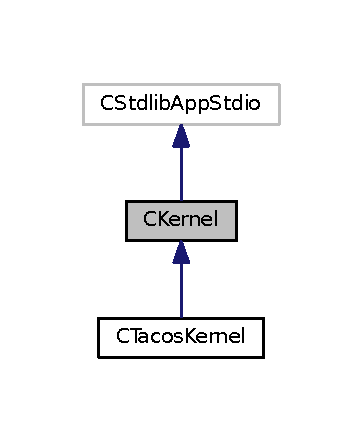
\includegraphics[width=174pt]{classCKernel__inherit__graph}
\end{center}
\end{figure}


Collaboration diagram for C\+Kernel\+:
\nopagebreak
\begin{figure}[H]
\begin{center}
\leavevmode
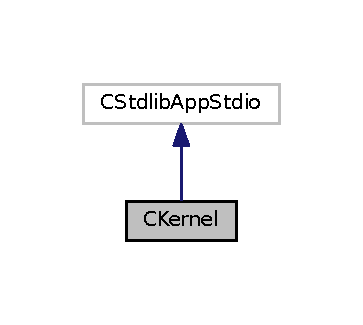
\includegraphics[width=174pt]{classCKernel__coll__graph}
\end{center}
\end{figure}
\subsection*{Public Member Functions}
\begin{DoxyCompactItemize}
\item 
\hyperlink{classCKernel_a06e0a6d15105f881c64b6a1c31ff9b81}{C\+Kernel} (void)
\item 
\hyperlink{kernel_8h_a1d97b873b27040859ad650950f96e569}{T\+Shutdown\+Mode} \hyperlink{classCKernel_a35b1e3c0aa496ac1eec6a70be56c1f6e}{Run} (void)
\item 
\hyperlink{classCKernel_a06e0a6d15105f881c64b6a1c31ff9b81}{C\+Kernel} (void)
\item 
\hyperlink{classCKernel_a127d8c2ddf52d6fc33b20a641b95ff18}{$\sim$\+C\+Kernel} (void)
\item 
boolean \hyperlink{classCKernel_ae767168897a124e4f24f5a3b2955c4f3}{Initialize} (void)
\item 
\hyperlink{kernel_8h_a1d97b873b27040859ad650950f96e569}{T\+Shutdown\+Mode} \hyperlink{classCKernel_a35b1e3c0aa496ac1eec6a70be56c1f6e}{Run} (void)
\end{DoxyCompactItemize}


\subsection{Constructor \& Destructor Documentation}
\index{C\+Kernel@{C\+Kernel}!C\+Kernel@{C\+Kernel}}
\index{C\+Kernel@{C\+Kernel}!C\+Kernel@{C\+Kernel}}
\subsubsection[{\texorpdfstring{C\+Kernel(void)}{CKernel(void)}}]{\setlength{\rightskip}{0pt plus 5cm}C\+Kernel\+::\+C\+Kernel (
\begin{DoxyParamCaption}
\item[{void}]{}
\end{DoxyParamCaption}
)}\hypertarget{classCKernel_a06e0a6d15105f881c64b6a1c31ff9b81}{}\label{classCKernel_a06e0a6d15105f881c64b6a1c31ff9b81}
\index{C\+Kernel@{C\+Kernel}!C\+Kernel@{C\+Kernel}}
\index{C\+Kernel@{C\+Kernel}!C\+Kernel@{C\+Kernel}}
\subsubsection[{\texorpdfstring{C\+Kernel(void)}{CKernel(void)}}]{\setlength{\rightskip}{0pt plus 5cm}C\+Kernel\+::\+C\+Kernel (
\begin{DoxyParamCaption}
\item[{void}]{}
\end{DoxyParamCaption}
)}\hypertarget{classCKernel_a06e0a6d15105f881c64b6a1c31ff9b81}{}\label{classCKernel_a06e0a6d15105f881c64b6a1c31ff9b81}
\index{C\+Kernel@{C\+Kernel}!````~C\+Kernel@{$\sim$\+C\+Kernel}}
\index{````~C\+Kernel@{$\sim$\+C\+Kernel}!C\+Kernel@{C\+Kernel}}
\subsubsection[{\texorpdfstring{$\sim$\+C\+Kernel(void)}{~CKernel(void)}}]{\setlength{\rightskip}{0pt plus 5cm}C\+Kernel\+::$\sim$\+C\+Kernel (
\begin{DoxyParamCaption}
\item[{void}]{}
\end{DoxyParamCaption}
)}\hypertarget{classCKernel_a127d8c2ddf52d6fc33b20a641b95ff18}{}\label{classCKernel_a127d8c2ddf52d6fc33b20a641b95ff18}


\subsection{Member Function Documentation}
\index{C\+Kernel@{C\+Kernel}!Initialize@{Initialize}}
\index{Initialize@{Initialize}!C\+Kernel@{C\+Kernel}}
\subsubsection[{\texorpdfstring{Initialize(void)}{Initialize(void)}}]{\setlength{\rightskip}{0pt plus 5cm}boolean C\+Kernel\+::\+Initialize (
\begin{DoxyParamCaption}
\item[{void}]{}
\end{DoxyParamCaption}
)}\hypertarget{classCKernel_ae767168897a124e4f24f5a3b2955c4f3}{}\label{classCKernel_ae767168897a124e4f24f5a3b2955c4f3}
\index{C\+Kernel@{C\+Kernel}!Run@{Run}}
\index{Run@{Run}!C\+Kernel@{C\+Kernel}}
\subsubsection[{\texorpdfstring{Run(void)}{Run(void)}}]{\setlength{\rightskip}{0pt plus 5cm}{\bf T\+Shutdown\+Mode} C\+Kernel\+::\+Run (
\begin{DoxyParamCaption}
\item[{void}]{}
\end{DoxyParamCaption}
)}\hypertarget{classCKernel_a35b1e3c0aa496ac1eec6a70be56c1f6e}{}\label{classCKernel_a35b1e3c0aa496ac1eec6a70be56c1f6e}
\index{C\+Kernel@{C\+Kernel}!Run@{Run}}
\index{Run@{Run}!C\+Kernel@{C\+Kernel}}
\subsubsection[{\texorpdfstring{Run(void)}{Run(void)}}]{\setlength{\rightskip}{0pt plus 5cm}{\bf T\+Shutdown\+Mode} C\+Kernel\+::\+Run (
\begin{DoxyParamCaption}
\item[{void}]{}
\end{DoxyParamCaption}
)}\hypertarget{classCKernel_a35b1e3c0aa496ac1eec6a70be56c1f6e}{}\label{classCKernel_a35b1e3c0aa496ac1eec6a70be56c1f6e}


The documentation for this class was generated from the following files\+:\begin{DoxyCompactItemize}
\item 
src/kernel/include/\hyperlink{arch_8h}{arch.\+h}\item 
sample/01-\/gpiosimple/\hyperlink{kernel_8h}{kernel.\+h}\item 
src/kernel/arch/rasp4/\hyperlink{arch_8cpp}{arch.\+cpp}\item 
sample/01-\/gpiosimple/\hyperlink{kernel_8cpp}{kernel.\+cpp}\end{DoxyCompactItemize}

\hypertarget{classCoreSchedule}{}\section{Core\+Schedule Class Reference}
\label{classCoreSchedule}\index{Core\+Schedule@{Core\+Schedule}}


{\ttfamily \#include $<$core\+\_\+schedule.\+hpp$>$}

\subsection*{Public Member Functions}
\begin{DoxyCompactItemize}
\item 
\hyperlink{classCoreSchedule_a98af6e7cc7713f8863a4d6565b62382a}{Core\+Schedule} (\hyperlink{core__schedule_8hpp_a3ecfdfd1095956ceceb46f208281f6ea}{Core\+Iterable} cores)
\end{DoxyCompactItemize}


\subsection{Constructor \& Destructor Documentation}
\index{Core\+Schedule@{Core\+Schedule}!Core\+Schedule@{Core\+Schedule}}
\index{Core\+Schedule@{Core\+Schedule}!Core\+Schedule@{Core\+Schedule}}
\subsubsection[{\texorpdfstring{Core\+Schedule(\+Core\+Iterable cores)}{CoreSchedule(CoreIterable cores)}}]{\setlength{\rightskip}{0pt plus 5cm}Core\+Schedule\+::\+Core\+Schedule (
\begin{DoxyParamCaption}
\item[{{\bf Core\+Iterable}}]{cores}
\end{DoxyParamCaption}
)\hspace{0.3cm}{\ttfamily [inline]}}\hypertarget{classCoreSchedule_a98af6e7cc7713f8863a4d6565b62382a}{}\label{classCoreSchedule_a98af6e7cc7713f8863a4d6565b62382a}


The documentation for this class was generated from the following file\+:\begin{DoxyCompactItemize}
\item 
src/types/include/\hyperlink{core__schedule_8hpp}{core\+\_\+schedule.\+hpp}\end{DoxyCompactItemize}

\hypertarget{classCTacosKernel}{}\section{C\+Tacos\+Kernel Class Reference}
\label{classCTacosKernel}\index{C\+Tacos\+Kernel@{C\+Tacos\+Kernel}}


{\ttfamily \#include $<$tacoskernel.\+h$>$}



Inheritance diagram for C\+Tacos\+Kernel\+:
\nopagebreak
\begin{figure}[H]
\begin{center}
\leavevmode
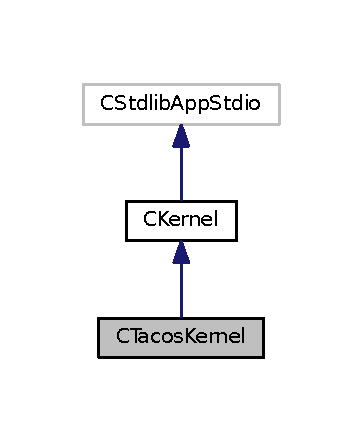
\includegraphics[width=174pt]{classCTacosKernel__inherit__graph}
\end{center}
\end{figure}


Collaboration diagram for C\+Tacos\+Kernel\+:
\nopagebreak
\begin{figure}[H]
\begin{center}
\leavevmode
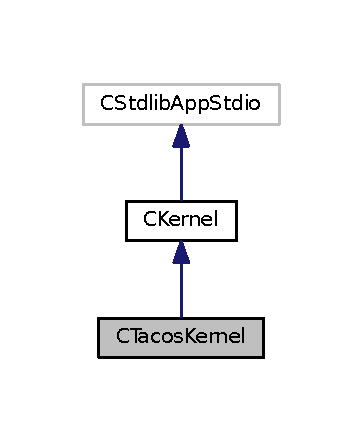
\includegraphics[width=174pt]{classCTacosKernel__coll__graph}
\end{center}
\end{figure}
\subsection*{Public Member Functions}
\begin{DoxyCompactItemize}
\item 
\hyperlink{classCTacosKernel_a4d0decf531f3ee25f184bb60046c898d}{C\+Tacos\+Kernel} ()
\item 
\hyperlink{kernel_8h_a1d97b873b27040859ad650950f96e569}{C\+Stdlib\+App\+::\+T\+Shutdown\+Mode} \hyperlink{classCTacosKernel_a860a684905062b7d6c6892437177e6fa}{Run} ()
\end{DoxyCompactItemize}


\subsection{Constructor \& Destructor Documentation}
\index{C\+Tacos\+Kernel@{C\+Tacos\+Kernel}!C\+Tacos\+Kernel@{C\+Tacos\+Kernel}}
\index{C\+Tacos\+Kernel@{C\+Tacos\+Kernel}!C\+Tacos\+Kernel@{C\+Tacos\+Kernel}}
\subsubsection[{\texorpdfstring{C\+Tacos\+Kernel()}{CTacosKernel()}}]{\setlength{\rightskip}{0pt plus 5cm}C\+Tacos\+Kernel\+::\+C\+Tacos\+Kernel (
\begin{DoxyParamCaption}
{}
\end{DoxyParamCaption}
)}\hypertarget{classCTacosKernel_a4d0decf531f3ee25f184bb60046c898d}{}\label{classCTacosKernel_a4d0decf531f3ee25f184bb60046c898d}


\subsection{Member Function Documentation}
\index{C\+Tacos\+Kernel@{C\+Tacos\+Kernel}!Run@{Run}}
\index{Run@{Run}!C\+Tacos\+Kernel@{C\+Tacos\+Kernel}}
\subsubsection[{\texorpdfstring{Run()}{Run()}}]{\setlength{\rightskip}{0pt plus 5cm}{\bf C\+Stdlib\+App\+::\+T\+Shutdown\+Mode} C\+Tacos\+Kernel\+::\+Run (
\begin{DoxyParamCaption}
\item[{void}]{}
\end{DoxyParamCaption}
)}\hypertarget{classCTacosKernel_a860a684905062b7d6c6892437177e6fa}{}\label{classCTacosKernel_a860a684905062b7d6c6892437177e6fa}


The documentation for this class was generated from the following files\+:\begin{DoxyCompactItemize}
\item 
src/kernel/core/\hyperlink{tacoskernel_8h}{tacoskernel.\+h}\item 
src/kernel/core/\hyperlink{tacoskernel_8cpp}{tacoskernel.\+cpp}\end{DoxyCompactItemize}

\hypertarget{structERROR__STATUS__TYPE}{}\section{E\+R\+R\+O\+R\+\_\+\+S\+T\+A\+T\+U\+S\+\_\+\+T\+Y\+PE Struct Reference}
\label{structERROR__STATUS__TYPE}\index{E\+R\+R\+O\+R\+\_\+\+S\+T\+A\+T\+U\+S\+\_\+\+T\+Y\+PE@{E\+R\+R\+O\+R\+\_\+\+S\+T\+A\+T\+U\+S\+\_\+\+T\+Y\+PE}}


{\ttfamily \#include $<$apex\+\_\+error.\+h$>$}

\subsection*{Public Attributes}
\begin{DoxyCompactItemize}
\item 
\hyperlink{apex__error_8h_a6c3334fe6390cd6a2e88e6a4aab5ffcc}{E\+R\+R\+O\+R\+\_\+\+C\+O\+D\+E\+\_\+\+T\+Y\+PE} \hyperlink{structERROR__STATUS__TYPE_a7e766892884aab7bc9830bc83bdfaa3b}{E\+R\+R\+O\+R\+\_\+\+C\+O\+DE}
\item 
\hyperlink{apex__error_8h_a0bec164d28637b1119fe1728e48262c2}{E\+R\+R\+O\+R\+\_\+\+M\+E\+S\+S\+A\+G\+E\+\_\+\+S\+I\+Z\+E\+\_\+\+T\+Y\+PE} \hyperlink{structERROR__STATUS__TYPE_a85fdbf6cbc8aaf3c4bcf7f05bf6ded21}{L\+E\+N\+G\+TH}
\item 
\hyperlink{apex__process_8h_a7a2c8e8d542c23599ac16fd978b241c4}{P\+R\+O\+C\+E\+S\+S\+\_\+\+I\+D\+\_\+\+T\+Y\+PE} \hyperlink{structERROR__STATUS__TYPE_a25a51bcff9ecdf57af3d59351c15503a}{F\+A\+I\+L\+E\+D\+\_\+\+P\+R\+O\+C\+E\+S\+S\+\_\+\+ID}
\item 
\hyperlink{apex__types_8h_afad87659fcb2bad73146a13b260290b9}{S\+Y\+S\+T\+E\+M\+\_\+\+A\+D\+D\+R\+E\+S\+S\+\_\+\+T\+Y\+PE} \hyperlink{structERROR__STATUS__TYPE_a24482299e857416957811845b37db84e}{F\+A\+I\+L\+E\+D\+\_\+\+A\+D\+D\+R\+E\+SS}
\item 
\hyperlink{apex__error_8h_a4b70f1f7793b79e3f25032ace3b04ff0}{E\+R\+R\+O\+R\+\_\+\+M\+E\+S\+S\+A\+G\+E\+\_\+\+T\+Y\+PE} \hyperlink{structERROR__STATUS__TYPE_a00202dd31a514e177d9bba92ee43d9d0}{M\+E\+S\+S\+A\+GE}
\end{DoxyCompactItemize}


\subsection{Member Data Documentation}
\index{E\+R\+R\+O\+R\+\_\+\+S\+T\+A\+T\+U\+S\+\_\+\+T\+Y\+PE@{E\+R\+R\+O\+R\+\_\+\+S\+T\+A\+T\+U\+S\+\_\+\+T\+Y\+PE}!E\+R\+R\+O\+R\+\_\+\+C\+O\+DE@{E\+R\+R\+O\+R\+\_\+\+C\+O\+DE}}
\index{E\+R\+R\+O\+R\+\_\+\+C\+O\+DE@{E\+R\+R\+O\+R\+\_\+\+C\+O\+DE}!E\+R\+R\+O\+R\+\_\+\+S\+T\+A\+T\+U\+S\+\_\+\+T\+Y\+PE@{E\+R\+R\+O\+R\+\_\+\+S\+T\+A\+T\+U\+S\+\_\+\+T\+Y\+PE}}
\subsubsection[{\texorpdfstring{E\+R\+R\+O\+R\+\_\+\+C\+O\+DE}{ERROR_CODE}}]{\setlength{\rightskip}{0pt plus 5cm}{\bf E\+R\+R\+O\+R\+\_\+\+C\+O\+D\+E\+\_\+\+T\+Y\+PE} E\+R\+R\+O\+R\+\_\+\+S\+T\+A\+T\+U\+S\+\_\+\+T\+Y\+P\+E\+::\+E\+R\+R\+O\+R\+\_\+\+C\+O\+DE}\hypertarget{structERROR__STATUS__TYPE_a7e766892884aab7bc9830bc83bdfaa3b}{}\label{structERROR__STATUS__TYPE_a7e766892884aab7bc9830bc83bdfaa3b}
\index{E\+R\+R\+O\+R\+\_\+\+S\+T\+A\+T\+U\+S\+\_\+\+T\+Y\+PE@{E\+R\+R\+O\+R\+\_\+\+S\+T\+A\+T\+U\+S\+\_\+\+T\+Y\+PE}!F\+A\+I\+L\+E\+D\+\_\+\+A\+D\+D\+R\+E\+SS@{F\+A\+I\+L\+E\+D\+\_\+\+A\+D\+D\+R\+E\+SS}}
\index{F\+A\+I\+L\+E\+D\+\_\+\+A\+D\+D\+R\+E\+SS@{F\+A\+I\+L\+E\+D\+\_\+\+A\+D\+D\+R\+E\+SS}!E\+R\+R\+O\+R\+\_\+\+S\+T\+A\+T\+U\+S\+\_\+\+T\+Y\+PE@{E\+R\+R\+O\+R\+\_\+\+S\+T\+A\+T\+U\+S\+\_\+\+T\+Y\+PE}}
\subsubsection[{\texorpdfstring{F\+A\+I\+L\+E\+D\+\_\+\+A\+D\+D\+R\+E\+SS}{FAILED_ADDRESS}}]{\setlength{\rightskip}{0pt plus 5cm}{\bf S\+Y\+S\+T\+E\+M\+\_\+\+A\+D\+D\+R\+E\+S\+S\+\_\+\+T\+Y\+PE} E\+R\+R\+O\+R\+\_\+\+S\+T\+A\+T\+U\+S\+\_\+\+T\+Y\+P\+E\+::\+F\+A\+I\+L\+E\+D\+\_\+\+A\+D\+D\+R\+E\+SS}\hypertarget{structERROR__STATUS__TYPE_a24482299e857416957811845b37db84e}{}\label{structERROR__STATUS__TYPE_a24482299e857416957811845b37db84e}
\index{E\+R\+R\+O\+R\+\_\+\+S\+T\+A\+T\+U\+S\+\_\+\+T\+Y\+PE@{E\+R\+R\+O\+R\+\_\+\+S\+T\+A\+T\+U\+S\+\_\+\+T\+Y\+PE}!F\+A\+I\+L\+E\+D\+\_\+\+P\+R\+O\+C\+E\+S\+S\+\_\+\+ID@{F\+A\+I\+L\+E\+D\+\_\+\+P\+R\+O\+C\+E\+S\+S\+\_\+\+ID}}
\index{F\+A\+I\+L\+E\+D\+\_\+\+P\+R\+O\+C\+E\+S\+S\+\_\+\+ID@{F\+A\+I\+L\+E\+D\+\_\+\+P\+R\+O\+C\+E\+S\+S\+\_\+\+ID}!E\+R\+R\+O\+R\+\_\+\+S\+T\+A\+T\+U\+S\+\_\+\+T\+Y\+PE@{E\+R\+R\+O\+R\+\_\+\+S\+T\+A\+T\+U\+S\+\_\+\+T\+Y\+PE}}
\subsubsection[{\texorpdfstring{F\+A\+I\+L\+E\+D\+\_\+\+P\+R\+O\+C\+E\+S\+S\+\_\+\+ID}{FAILED_PROCESS_ID}}]{\setlength{\rightskip}{0pt plus 5cm}{\bf P\+R\+O\+C\+E\+S\+S\+\_\+\+I\+D\+\_\+\+T\+Y\+PE} E\+R\+R\+O\+R\+\_\+\+S\+T\+A\+T\+U\+S\+\_\+\+T\+Y\+P\+E\+::\+F\+A\+I\+L\+E\+D\+\_\+\+P\+R\+O\+C\+E\+S\+S\+\_\+\+ID}\hypertarget{structERROR__STATUS__TYPE_a25a51bcff9ecdf57af3d59351c15503a}{}\label{structERROR__STATUS__TYPE_a25a51bcff9ecdf57af3d59351c15503a}
\index{E\+R\+R\+O\+R\+\_\+\+S\+T\+A\+T\+U\+S\+\_\+\+T\+Y\+PE@{E\+R\+R\+O\+R\+\_\+\+S\+T\+A\+T\+U\+S\+\_\+\+T\+Y\+PE}!L\+E\+N\+G\+TH@{L\+E\+N\+G\+TH}}
\index{L\+E\+N\+G\+TH@{L\+E\+N\+G\+TH}!E\+R\+R\+O\+R\+\_\+\+S\+T\+A\+T\+U\+S\+\_\+\+T\+Y\+PE@{E\+R\+R\+O\+R\+\_\+\+S\+T\+A\+T\+U\+S\+\_\+\+T\+Y\+PE}}
\subsubsection[{\texorpdfstring{L\+E\+N\+G\+TH}{LENGTH}}]{\setlength{\rightskip}{0pt plus 5cm}{\bf E\+R\+R\+O\+R\+\_\+\+M\+E\+S\+S\+A\+G\+E\+\_\+\+S\+I\+Z\+E\+\_\+\+T\+Y\+PE} E\+R\+R\+O\+R\+\_\+\+S\+T\+A\+T\+U\+S\+\_\+\+T\+Y\+P\+E\+::\+L\+E\+N\+G\+TH}\hypertarget{structERROR__STATUS__TYPE_a85fdbf6cbc8aaf3c4bcf7f05bf6ded21}{}\label{structERROR__STATUS__TYPE_a85fdbf6cbc8aaf3c4bcf7f05bf6ded21}
\index{E\+R\+R\+O\+R\+\_\+\+S\+T\+A\+T\+U\+S\+\_\+\+T\+Y\+PE@{E\+R\+R\+O\+R\+\_\+\+S\+T\+A\+T\+U\+S\+\_\+\+T\+Y\+PE}!M\+E\+S\+S\+A\+GE@{M\+E\+S\+S\+A\+GE}}
\index{M\+E\+S\+S\+A\+GE@{M\+E\+S\+S\+A\+GE}!E\+R\+R\+O\+R\+\_\+\+S\+T\+A\+T\+U\+S\+\_\+\+T\+Y\+PE@{E\+R\+R\+O\+R\+\_\+\+S\+T\+A\+T\+U\+S\+\_\+\+T\+Y\+PE}}
\subsubsection[{\texorpdfstring{M\+E\+S\+S\+A\+GE}{MESSAGE}}]{\setlength{\rightskip}{0pt plus 5cm}{\bf E\+R\+R\+O\+R\+\_\+\+M\+E\+S\+S\+A\+G\+E\+\_\+\+T\+Y\+PE} E\+R\+R\+O\+R\+\_\+\+S\+T\+A\+T\+U\+S\+\_\+\+T\+Y\+P\+E\+::\+M\+E\+S\+S\+A\+GE}\hypertarget{structERROR__STATUS__TYPE_a00202dd31a514e177d9bba92ee43d9d0}{}\label{structERROR__STATUS__TYPE_a00202dd31a514e177d9bba92ee43d9d0}


The documentation for this struct was generated from the following file\+:\begin{DoxyCompactItemize}
\item 
src/libuser/apex/\hyperlink{apex__error_8h}{apex\+\_\+error.\+h}\end{DoxyCompactItemize}

\hypertarget{classErrorLevel}{}\section{Error\+Level Class Reference}
\label{classErrorLevel}\index{Error\+Level@{Error\+Level}}


{\ttfamily \#include $<$error\+\_\+level.\+hpp$>$}

\subsection*{Public Member Functions}
\begin{DoxyCompactItemize}
\item 
\hyperlink{classErrorLevel_a2a506dd351dd5f79b1f8cac435c95423}{Error\+Level} ()
\item 
\hyperlink{classErrorLevel_ae8999dee8b9cf6a27b545b705e031f40}{Error\+Level} (\hyperlink{general__types_8hpp_a824b78b06da8112c2772bc666a63638d}{identifier\+\_\+t} id, \hyperlink{structname__t}{name\+\_\+t} description, \hyperlink{apex__error_8h_aa4da4218c0e2dcb8c37ea7a6cb5bd515}{E\+R\+R\+O\+R\+\_\+\+L\+E\+V\+E\+L\+\_\+\+T\+Y\+PE} level, \hyperlink{apex__error_8h_a6c3334fe6390cd6a2e88e6a4aab5ffcc}{E\+R\+R\+O\+R\+\_\+\+C\+O\+D\+E\+\_\+\+T\+Y\+PE} code)
\item 
const \hyperlink{general__types_8hpp_a824b78b06da8112c2772bc666a63638d}{identifier\+\_\+t} \& \hyperlink{classErrorLevel_aeabf1a1b8868cb8c2dad90b4d9441ee5}{get\+Error\+Identifier} () const 
\item 
const std\+::optional$<$ \hyperlink{structname__t}{name\+\_\+t} $>$ \& \hyperlink{classErrorLevel_a9ca8a1d4ca9dc4360eafa7eb5c9d9c2f}{get\+Description} () const 
\item 
const \hyperlink{apex__error_8h_aa4da4218c0e2dcb8c37ea7a6cb5bd515}{E\+R\+R\+O\+R\+\_\+\+L\+E\+V\+E\+L\+\_\+\+T\+Y\+PE} \& \hyperlink{classErrorLevel_a794f6ce5cf346c11951539464bb742cf}{get\+Error\+Level} () const 
\item 
const std\+::optional$<$ \hyperlink{apex__error_8h_a6c3334fe6390cd6a2e88e6a4aab5ffcc}{E\+R\+R\+O\+R\+\_\+\+C\+O\+D\+E\+\_\+\+T\+Y\+PE} $>$ \& \hyperlink{classErrorLevel_aace829e4a499b5ec630b7ff1e2608853}{get\+Error\+Code} () const 
\end{DoxyCompactItemize}


\subsection{Constructor \& Destructor Documentation}
\index{Error\+Level@{Error\+Level}!Error\+Level@{Error\+Level}}
\index{Error\+Level@{Error\+Level}!Error\+Level@{Error\+Level}}
\subsubsection[{\texorpdfstring{Error\+Level()}{ErrorLevel()}}]{\setlength{\rightskip}{0pt plus 5cm}Error\+Level\+::\+Error\+Level (
\begin{DoxyParamCaption}
{}
\end{DoxyParamCaption}
)\hspace{0.3cm}{\ttfamily [inline]}}\hypertarget{classErrorLevel_a2a506dd351dd5f79b1f8cac435c95423}{}\label{classErrorLevel_a2a506dd351dd5f79b1f8cac435c95423}
\index{Error\+Level@{Error\+Level}!Error\+Level@{Error\+Level}}
\index{Error\+Level@{Error\+Level}!Error\+Level@{Error\+Level}}
\subsubsection[{\texorpdfstring{Error\+Level(identifier\+\_\+t id, name\+\_\+t description, E\+R\+R\+O\+R\+\_\+\+L\+E\+V\+E\+L\+\_\+\+T\+Y\+P\+E level, E\+R\+R\+O\+R\+\_\+\+C\+O\+D\+E\+\_\+\+T\+Y\+P\+E code)}{ErrorLevel(identifier_t id, name_t description, ERROR_LEVEL_TYPE level, ERROR_CODE_TYPE code)}}]{\setlength{\rightskip}{0pt plus 5cm}Error\+Level\+::\+Error\+Level (
\begin{DoxyParamCaption}
\item[{{\bf identifier\+\_\+t}}]{id, }
\item[{{\bf name\+\_\+t}}]{description, }
\item[{{\bf E\+R\+R\+O\+R\+\_\+\+L\+E\+V\+E\+L\+\_\+\+T\+Y\+PE}}]{level, }
\item[{{\bf E\+R\+R\+O\+R\+\_\+\+C\+O\+D\+E\+\_\+\+T\+Y\+PE}}]{code}
\end{DoxyParamCaption}
)\hspace{0.3cm}{\ttfamily [inline]}}\hypertarget{classErrorLevel_ae8999dee8b9cf6a27b545b705e031f40}{}\label{classErrorLevel_ae8999dee8b9cf6a27b545b705e031f40}


\subsection{Member Function Documentation}
\index{Error\+Level@{Error\+Level}!get\+Description@{get\+Description}}
\index{get\+Description@{get\+Description}!Error\+Level@{Error\+Level}}
\subsubsection[{\texorpdfstring{get\+Description() const }{getDescription() const }}]{\setlength{\rightskip}{0pt plus 5cm}const std\+::optional$<$ {\bf name\+\_\+t} $>$ \& Error\+Level\+::get\+Description (
\begin{DoxyParamCaption}
{}
\end{DoxyParamCaption}
) const}\hypertarget{classErrorLevel_a9ca8a1d4ca9dc4360eafa7eb5c9d9c2f}{}\label{classErrorLevel_a9ca8a1d4ca9dc4360eafa7eb5c9d9c2f}
\index{Error\+Level@{Error\+Level}!get\+Error\+Code@{get\+Error\+Code}}
\index{get\+Error\+Code@{get\+Error\+Code}!Error\+Level@{Error\+Level}}
\subsubsection[{\texorpdfstring{get\+Error\+Code() const }{getErrorCode() const }}]{\setlength{\rightskip}{0pt plus 5cm}const std\+::optional$<$ {\bf E\+R\+R\+O\+R\+\_\+\+C\+O\+D\+E\+\_\+\+T\+Y\+PE} $>$ \& Error\+Level\+::get\+Error\+Code (
\begin{DoxyParamCaption}
{}
\end{DoxyParamCaption}
) const}\hypertarget{classErrorLevel_aace829e4a499b5ec630b7ff1e2608853}{}\label{classErrorLevel_aace829e4a499b5ec630b7ff1e2608853}
\index{Error\+Level@{Error\+Level}!get\+Error\+Identifier@{get\+Error\+Identifier}}
\index{get\+Error\+Identifier@{get\+Error\+Identifier}!Error\+Level@{Error\+Level}}
\subsubsection[{\texorpdfstring{get\+Error\+Identifier() const }{getErrorIdentifier() const }}]{\setlength{\rightskip}{0pt plus 5cm}const {\bf identifier\+\_\+t} \& Error\+Level\+::get\+Error\+Identifier (
\begin{DoxyParamCaption}
{}
\end{DoxyParamCaption}
) const}\hypertarget{classErrorLevel_aeabf1a1b8868cb8c2dad90b4d9441ee5}{}\label{classErrorLevel_aeabf1a1b8868cb8c2dad90b4d9441ee5}
\index{Error\+Level@{Error\+Level}!get\+Error\+Level@{get\+Error\+Level}}
\index{get\+Error\+Level@{get\+Error\+Level}!Error\+Level@{Error\+Level}}
\subsubsection[{\texorpdfstring{get\+Error\+Level() const }{getErrorLevel() const }}]{\setlength{\rightskip}{0pt plus 5cm}const {\bf E\+R\+R\+O\+R\+\_\+\+L\+E\+V\+E\+L\+\_\+\+T\+Y\+PE} \& Error\+Level\+::get\+Error\+Level (
\begin{DoxyParamCaption}
{}
\end{DoxyParamCaption}
) const}\hypertarget{classErrorLevel_a794f6ce5cf346c11951539464bb742cf}{}\label{classErrorLevel_a794f6ce5cf346c11951539464bb742cf}


The documentation for this class was generated from the following files\+:\begin{DoxyCompactItemize}
\item 
src/types/include/\hyperlink{error__level_8hpp}{error\+\_\+level.\+hpp}\item 
src/types/src/\hyperlink{error__level_8cpp}{error\+\_\+level.\+cpp}\end{DoxyCompactItemize}

\hypertarget{structEVENT__STATUS__TYPE}{}\section{E\+V\+E\+N\+T\+\_\+\+S\+T\+A\+T\+U\+S\+\_\+\+T\+Y\+PE Struct Reference}
\label{structEVENT__STATUS__TYPE}\index{E\+V\+E\+N\+T\+\_\+\+S\+T\+A\+T\+U\+S\+\_\+\+T\+Y\+PE@{E\+V\+E\+N\+T\+\_\+\+S\+T\+A\+T\+U\+S\+\_\+\+T\+Y\+PE}}


{\ttfamily \#include $<$apex\+\_\+event.\+h$>$}

\subsection*{Public Attributes}
\begin{DoxyCompactItemize}
\item 
\hyperlink{apex__event_8h_a2629ecda01c112ff228d24d2c19891b5}{E\+V\+E\+N\+T\+\_\+\+S\+T\+A\+T\+E\+\_\+\+T\+Y\+PE} \hyperlink{structEVENT__STATUS__TYPE_a38a5d36398ae4fc078629958cca606f3}{E\+V\+E\+N\+T\+\_\+\+S\+T\+A\+TE}
\item 
\hyperlink{apex__process_8h_a77a39a661169092676366eec0d65ab1c}{W\+A\+I\+T\+I\+N\+G\+\_\+\+R\+A\+N\+G\+E\+\_\+\+T\+Y\+PE} \hyperlink{structEVENT__STATUS__TYPE_a298376f128a83534e4ddef39ed78664e}{W\+A\+I\+T\+I\+N\+G\+\_\+\+P\+R\+O\+C\+E\+S\+S\+ES}
\end{DoxyCompactItemize}


\subsection{Member Data Documentation}
\index{E\+V\+E\+N\+T\+\_\+\+S\+T\+A\+T\+U\+S\+\_\+\+T\+Y\+PE@{E\+V\+E\+N\+T\+\_\+\+S\+T\+A\+T\+U\+S\+\_\+\+T\+Y\+PE}!E\+V\+E\+N\+T\+\_\+\+S\+T\+A\+TE@{E\+V\+E\+N\+T\+\_\+\+S\+T\+A\+TE}}
\index{E\+V\+E\+N\+T\+\_\+\+S\+T\+A\+TE@{E\+V\+E\+N\+T\+\_\+\+S\+T\+A\+TE}!E\+V\+E\+N\+T\+\_\+\+S\+T\+A\+T\+U\+S\+\_\+\+T\+Y\+PE@{E\+V\+E\+N\+T\+\_\+\+S\+T\+A\+T\+U\+S\+\_\+\+T\+Y\+PE}}
\subsubsection[{\texorpdfstring{E\+V\+E\+N\+T\+\_\+\+S\+T\+A\+TE}{EVENT_STATE}}]{\setlength{\rightskip}{0pt plus 5cm}{\bf E\+V\+E\+N\+T\+\_\+\+S\+T\+A\+T\+E\+\_\+\+T\+Y\+PE} E\+V\+E\+N\+T\+\_\+\+S\+T\+A\+T\+U\+S\+\_\+\+T\+Y\+P\+E\+::\+E\+V\+E\+N\+T\+\_\+\+S\+T\+A\+TE}\hypertarget{structEVENT__STATUS__TYPE_a38a5d36398ae4fc078629958cca606f3}{}\label{structEVENT__STATUS__TYPE_a38a5d36398ae4fc078629958cca606f3}
\index{E\+V\+E\+N\+T\+\_\+\+S\+T\+A\+T\+U\+S\+\_\+\+T\+Y\+PE@{E\+V\+E\+N\+T\+\_\+\+S\+T\+A\+T\+U\+S\+\_\+\+T\+Y\+PE}!W\+A\+I\+T\+I\+N\+G\+\_\+\+P\+R\+O\+C\+E\+S\+S\+ES@{W\+A\+I\+T\+I\+N\+G\+\_\+\+P\+R\+O\+C\+E\+S\+S\+ES}}
\index{W\+A\+I\+T\+I\+N\+G\+\_\+\+P\+R\+O\+C\+E\+S\+S\+ES@{W\+A\+I\+T\+I\+N\+G\+\_\+\+P\+R\+O\+C\+E\+S\+S\+ES}!E\+V\+E\+N\+T\+\_\+\+S\+T\+A\+T\+U\+S\+\_\+\+T\+Y\+PE@{E\+V\+E\+N\+T\+\_\+\+S\+T\+A\+T\+U\+S\+\_\+\+T\+Y\+PE}}
\subsubsection[{\texorpdfstring{W\+A\+I\+T\+I\+N\+G\+\_\+\+P\+R\+O\+C\+E\+S\+S\+ES}{WAITING_PROCESSES}}]{\setlength{\rightskip}{0pt plus 5cm}{\bf W\+A\+I\+T\+I\+N\+G\+\_\+\+R\+A\+N\+G\+E\+\_\+\+T\+Y\+PE} E\+V\+E\+N\+T\+\_\+\+S\+T\+A\+T\+U\+S\+\_\+\+T\+Y\+P\+E\+::\+W\+A\+I\+T\+I\+N\+G\+\_\+\+P\+R\+O\+C\+E\+S\+S\+ES}\hypertarget{structEVENT__STATUS__TYPE_a298376f128a83534e4ddef39ed78664e}{}\label{structEVENT__STATUS__TYPE_a298376f128a83534e4ddef39ed78664e}


The documentation for this struct was generated from the following file\+:\begin{DoxyCompactItemize}
\item 
src/libuser/apex/\hyperlink{apex__event_8h}{apex\+\_\+event.\+h}\end{DoxyCompactItemize}

\hypertarget{classIProcess}{}\section{I\+Process Class Reference}
\label{classIProcess}\index{I\+Process@{I\+Process}}


{\ttfamily \#include $<$processinterface.\+h$>$}



Inheritance diagram for I\+Process\+:
\nopagebreak
\begin{figure}[H]
\begin{center}
\leavevmode
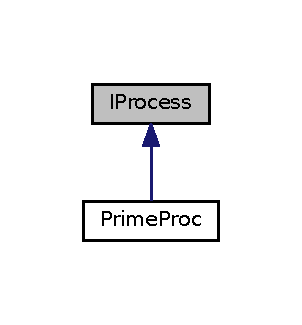
\includegraphics[width=145pt]{classIProcess__inherit__graph}
\end{center}
\end{figure}
\subsection*{Public Member Functions}
\begin{DoxyCompactItemize}
\item 
\hyperlink{classIProcess_a9718ec3b13da2c71322bb32d703cb618}{I\+Process} (const char $\ast$name)
\item 
virtual \hyperlink{classIProcess_af9ed5e42aa4c8d489d45a25a278434e1}{$\sim$\+I\+Process} ()
\item 
virtual void \hyperlink{classIProcess_ae2a840bd8730af48b04254387ba3f9e3}{run} ()=0
\item 
virtual bool \hyperlink{classIProcess_a238bce621ce9e6cf7c9dc4201bdfb8b2}{initialise} ()=0
\end{DoxyCompactItemize}
\subsection*{Protected Attributes}
\begin{DoxyCompactItemize}
\item 
const char $\ast$ \hyperlink{classIProcess_ad8e9a2d6537a7671236456af14b3a5b7}{name\+Ref}
\end{DoxyCompactItemize}


\subsection{Constructor \& Destructor Documentation}
\index{I\+Process@{I\+Process}!I\+Process@{I\+Process}}
\index{I\+Process@{I\+Process}!I\+Process@{I\+Process}}
\subsubsection[{\texorpdfstring{I\+Process(const char $\ast$name)}{IProcess(const char *name)}}]{\setlength{\rightskip}{0pt plus 5cm}I\+Process\+::\+I\+Process (
\begin{DoxyParamCaption}
\item[{const char $\ast$}]{name}
\end{DoxyParamCaption}
)\hspace{0.3cm}{\ttfamily [inline]}}\hypertarget{classIProcess_a9718ec3b13da2c71322bb32d703cb618}{}\label{classIProcess_a9718ec3b13da2c71322bb32d703cb618}
\index{I\+Process@{I\+Process}!````~I\+Process@{$\sim$\+I\+Process}}
\index{````~I\+Process@{$\sim$\+I\+Process}!I\+Process@{I\+Process}}
\subsubsection[{\texorpdfstring{$\sim$\+I\+Process()}{~IProcess()}}]{\setlength{\rightskip}{0pt plus 5cm}virtual I\+Process\+::$\sim$\+I\+Process (
\begin{DoxyParamCaption}
{}
\end{DoxyParamCaption}
)\hspace{0.3cm}{\ttfamily [inline]}, {\ttfamily [virtual]}}\hypertarget{classIProcess_af9ed5e42aa4c8d489d45a25a278434e1}{}\label{classIProcess_af9ed5e42aa4c8d489d45a25a278434e1}


\subsection{Member Function Documentation}
\index{I\+Process@{I\+Process}!initialise@{initialise}}
\index{initialise@{initialise}!I\+Process@{I\+Process}}
\subsubsection[{\texorpdfstring{initialise()=0}{initialise()=0}}]{\setlength{\rightskip}{0pt plus 5cm}virtual bool I\+Process\+::initialise (
\begin{DoxyParamCaption}
{}
\end{DoxyParamCaption}
)\hspace{0.3cm}{\ttfamily [pure virtual]}}\hypertarget{classIProcess_a238bce621ce9e6cf7c9dc4201bdfb8b2}{}\label{classIProcess_a238bce621ce9e6cf7c9dc4201bdfb8b2}


Implemented in \hyperlink{classPrimeProc_ac8b98010d54586414e26f84aec7c9067}{Prime\+Proc}.

\index{I\+Process@{I\+Process}!run@{run}}
\index{run@{run}!I\+Process@{I\+Process}}
\subsubsection[{\texorpdfstring{run()=0}{run()=0}}]{\setlength{\rightskip}{0pt plus 5cm}virtual void I\+Process\+::run (
\begin{DoxyParamCaption}
{}
\end{DoxyParamCaption}
)\hspace{0.3cm}{\ttfamily [pure virtual]}}\hypertarget{classIProcess_ae2a840bd8730af48b04254387ba3f9e3}{}\label{classIProcess_ae2a840bd8730af48b04254387ba3f9e3}


Implemented in \hyperlink{classPrimeProc_a650b1ea0ed282f5137b594a8f916990a}{Prime\+Proc}.



\subsection{Member Data Documentation}
\index{I\+Process@{I\+Process}!name\+Ref@{name\+Ref}}
\index{name\+Ref@{name\+Ref}!I\+Process@{I\+Process}}
\subsubsection[{\texorpdfstring{name\+Ref}{nameRef}}]{\setlength{\rightskip}{0pt plus 5cm}const char$\ast$ I\+Process\+::name\+Ref\hspace{0.3cm}{\ttfamily [protected]}}\hypertarget{classIProcess_ad8e9a2d6537a7671236456af14b3a5b7}{}\label{classIProcess_ad8e9a2d6537a7671236456af14b3a5b7}


The documentation for this class was generated from the following file\+:\begin{DoxyCompactItemize}
\item 
src/kernel/core/process/\hyperlink{processinterface_8h}{processinterface.\+h}\end{DoxyCompactItemize}

\hypertarget{classMemoryRegion}{}\section{Memory\+Region Class Reference}
\label{classMemoryRegion}\index{Memory\+Region@{Memory\+Region}}


{\ttfamily \#include $<$memory\+\_\+requirements.\+hpp$>$}

\subsection*{Public Member Functions}
\begin{DoxyCompactItemize}
\item 
\hyperlink{classMemoryRegion_a2cfe313fec204b9ae6010fb28bab02be}{Memory\+Region} ()
\item 
\hyperlink{classMemoryRegion_a7fa5ab5ab3defa36270571ad3e2a1b2d}{Memory\+Region} (\hyperlink{structname__t}{name\+\_\+t} name, \hyperlink{memory__requirements_8hpp_a306cba03fa0fb72d807fc29d19376ead}{memory\+\_\+region\+\_\+t} type, \hyperlink{general__types_8hpp_a0edc3a86ddf4aa205c6882b61cd7b4e9}{dec\+Or\+Hex\+\_\+t} size, \hyperlink{memory__requirements_8hpp_a2ac65df2063d231ce475db7ef11ef039}{memory\+\_\+access\+\_\+t} access\+Rights, \hyperlink{general__types_8hpp_a0edc3a86ddf4aa205c6882b61cd7b4e9}{dec\+Or\+Hex\+\_\+t} address)
\item 
const \hyperlink{structname__t}{name\+\_\+t} \& \hyperlink{classMemoryRegion_a9d62e8cea8d7064fe787994351bc06fd}{get\+Region\+Name} () const 
\item 
const \hyperlink{memory__requirements_8hpp_a306cba03fa0fb72d807fc29d19376ead}{memory\+\_\+region\+\_\+t} \& \hyperlink{classMemoryRegion_afb0f6a097108c5cb1e1d7f26b7258ae2}{get\+Type} () const 
\item 
const \hyperlink{general__types_8hpp_a0edc3a86ddf4aa205c6882b61cd7b4e9}{dec\+Or\+Hex\+\_\+t} \& \hyperlink{classMemoryRegion_a4fc497b2f396152830e493e2303f3629}{get\+Size} () const 
\item 
const \hyperlink{memory__requirements_8hpp_a2ac65df2063d231ce475db7ef11ef039}{memory\+\_\+access\+\_\+t} \& \hyperlink{classMemoryRegion_ae5df8d0b9a94e4e8ce3acb7a365e4722}{get\+Access\+Rights} () const 
\item 
const std\+::optional$<$ \hyperlink{general__types_8hpp_a0edc3a86ddf4aa205c6882b61cd7b4e9}{dec\+Or\+Hex\+\_\+t} $>$ \& \hyperlink{classMemoryRegion_aebbaa6c7baf7bb6fbf01cc6607587aaa}{get\+Address} () const 
\end{DoxyCompactItemize}


\subsection{Constructor \& Destructor Documentation}
\index{Memory\+Region@{Memory\+Region}!Memory\+Region@{Memory\+Region}}
\index{Memory\+Region@{Memory\+Region}!Memory\+Region@{Memory\+Region}}
\subsubsection[{\texorpdfstring{Memory\+Region()}{MemoryRegion()}}]{\setlength{\rightskip}{0pt plus 5cm}Memory\+Region\+::\+Memory\+Region (
\begin{DoxyParamCaption}
{}
\end{DoxyParamCaption}
)\hspace{0.3cm}{\ttfamily [inline]}}\hypertarget{classMemoryRegion_a2cfe313fec204b9ae6010fb28bab02be}{}\label{classMemoryRegion_a2cfe313fec204b9ae6010fb28bab02be}
\index{Memory\+Region@{Memory\+Region}!Memory\+Region@{Memory\+Region}}
\index{Memory\+Region@{Memory\+Region}!Memory\+Region@{Memory\+Region}}
\subsubsection[{\texorpdfstring{Memory\+Region(name\+\_\+t name, memory\+\_\+region\+\_\+t type, dec\+Or\+Hex\+\_\+t size, memory\+\_\+access\+\_\+t access\+Rights, dec\+Or\+Hex\+\_\+t address)}{MemoryRegion(name_t name, memory_region_t type, decOrHex_t size, memory_access_t accessRights, decOrHex_t address)}}]{\setlength{\rightskip}{0pt plus 5cm}Memory\+Region\+::\+Memory\+Region (
\begin{DoxyParamCaption}
\item[{{\bf name\+\_\+t}}]{name, }
\item[{{\bf memory\+\_\+region\+\_\+t}}]{type, }
\item[{{\bf dec\+Or\+Hex\+\_\+t}}]{size, }
\item[{{\bf memory\+\_\+access\+\_\+t}}]{access\+Rights, }
\item[{{\bf dec\+Or\+Hex\+\_\+t}}]{address}
\end{DoxyParamCaption}
)\hspace{0.3cm}{\ttfamily [inline]}}\hypertarget{classMemoryRegion_a7fa5ab5ab3defa36270571ad3e2a1b2d}{}\label{classMemoryRegion_a7fa5ab5ab3defa36270571ad3e2a1b2d}


\subsection{Member Function Documentation}
\index{Memory\+Region@{Memory\+Region}!get\+Access\+Rights@{get\+Access\+Rights}}
\index{get\+Access\+Rights@{get\+Access\+Rights}!Memory\+Region@{Memory\+Region}}
\subsubsection[{\texorpdfstring{get\+Access\+Rights() const }{getAccessRights() const }}]{\setlength{\rightskip}{0pt plus 5cm}const {\bf memory\+\_\+access\+\_\+t} \& Memory\+Region\+::get\+Access\+Rights (
\begin{DoxyParamCaption}
{}
\end{DoxyParamCaption}
) const}\hypertarget{classMemoryRegion_ae5df8d0b9a94e4e8ce3acb7a365e4722}{}\label{classMemoryRegion_ae5df8d0b9a94e4e8ce3acb7a365e4722}
\index{Memory\+Region@{Memory\+Region}!get\+Address@{get\+Address}}
\index{get\+Address@{get\+Address}!Memory\+Region@{Memory\+Region}}
\subsubsection[{\texorpdfstring{get\+Address() const }{getAddress() const }}]{\setlength{\rightskip}{0pt plus 5cm}const std\+::optional$<$ {\bf dec\+Or\+Hex\+\_\+t} $>$ \& Memory\+Region\+::get\+Address (
\begin{DoxyParamCaption}
{}
\end{DoxyParamCaption}
) const}\hypertarget{classMemoryRegion_aebbaa6c7baf7bb6fbf01cc6607587aaa}{}\label{classMemoryRegion_aebbaa6c7baf7bb6fbf01cc6607587aaa}
\index{Memory\+Region@{Memory\+Region}!get\+Region\+Name@{get\+Region\+Name}}
\index{get\+Region\+Name@{get\+Region\+Name}!Memory\+Region@{Memory\+Region}}
\subsubsection[{\texorpdfstring{get\+Region\+Name() const }{getRegionName() const }}]{\setlength{\rightskip}{0pt plus 5cm}const {\bf name\+\_\+t} \& Memory\+Region\+::get\+Region\+Name (
\begin{DoxyParamCaption}
{}
\end{DoxyParamCaption}
) const}\hypertarget{classMemoryRegion_a9d62e8cea8d7064fe787994351bc06fd}{}\label{classMemoryRegion_a9d62e8cea8d7064fe787994351bc06fd}
\index{Memory\+Region@{Memory\+Region}!get\+Size@{get\+Size}}
\index{get\+Size@{get\+Size}!Memory\+Region@{Memory\+Region}}
\subsubsection[{\texorpdfstring{get\+Size() const }{getSize() const }}]{\setlength{\rightskip}{0pt plus 5cm}const {\bf dec\+Or\+Hex\+\_\+t} \& Memory\+Region\+::get\+Size (
\begin{DoxyParamCaption}
{}
\end{DoxyParamCaption}
) const}\hypertarget{classMemoryRegion_a4fc497b2f396152830e493e2303f3629}{}\label{classMemoryRegion_a4fc497b2f396152830e493e2303f3629}
\index{Memory\+Region@{Memory\+Region}!get\+Type@{get\+Type}}
\index{get\+Type@{get\+Type}!Memory\+Region@{Memory\+Region}}
\subsubsection[{\texorpdfstring{get\+Type() const }{getType() const }}]{\setlength{\rightskip}{0pt plus 5cm}const {\bf memory\+\_\+region\+\_\+t} \& Memory\+Region\+::get\+Type (
\begin{DoxyParamCaption}
{}
\end{DoxyParamCaption}
) const}\hypertarget{classMemoryRegion_afb0f6a097108c5cb1e1d7f26b7258ae2}{}\label{classMemoryRegion_afb0f6a097108c5cb1e1d7f26b7258ae2}


The documentation for this class was generated from the following files\+:\begin{DoxyCompactItemize}
\item 
src/types/include/\hyperlink{memory__requirements_8hpp}{memory\+\_\+requirements.\+hpp}\item 
src/types/src/\hyperlink{memory__requirements_8cpp}{memory\+\_\+requirements.\+cpp}\end{DoxyCompactItemize}

\hypertarget{classModuleErrorAction}{}\section{Module\+Error\+Action Class Reference}
\label{classModuleErrorAction}\index{Module\+Error\+Action@{Module\+Error\+Action}}


{\ttfamily \#include $<$module\+\_\+error\+\_\+action.\+hpp$>$}

\subsection*{Public Member Functions}
\begin{DoxyCompactItemize}
\item 
\hyperlink{classModuleErrorAction_adb80262b2edf34ceb40e7e64f23b347a}{Module\+Error\+Action} ()
\item 
\hyperlink{classModuleErrorAction_ae1395514e50787f321025620fb9f7ef2}{Module\+Error\+Action} (\hyperlink{general__types_8hpp_a824b78b06da8112c2772bc666a63638d}{identifier\+\_\+t} id, \hyperlink{apex__error_8h_aecf7a2a9c5fb5be7125e5c9eb6d67023}{M\+O\+D\+U\+L\+E\+\_\+\+R\+E\+C\+O\+V\+E\+R\+Y\+\_\+\+A\+C\+T\+I\+O\+N\+\_\+\+T\+Y\+PE} action)
\item 
const \hyperlink{general__types_8hpp_a824b78b06da8112c2772bc666a63638d}{identifier\+\_\+t} \& \hyperlink{classModuleErrorAction_a44235b72c1d835ade03c3e307c3da078}{get\+Error\+Identifier} () const 
\item 
const \hyperlink{apex__error_8h_aecf7a2a9c5fb5be7125e5c9eb6d67023}{M\+O\+D\+U\+L\+E\+\_\+\+R\+E\+C\+O\+V\+E\+R\+Y\+\_\+\+A\+C\+T\+I\+O\+N\+\_\+\+T\+Y\+PE} \& \hyperlink{classModuleErrorAction_adcfe053b57d3210aae2c8c9cba9fd5bc}{get\+Action} () const 
\end{DoxyCompactItemize}


\subsection{Constructor \& Destructor Documentation}
\index{Module\+Error\+Action@{Module\+Error\+Action}!Module\+Error\+Action@{Module\+Error\+Action}}
\index{Module\+Error\+Action@{Module\+Error\+Action}!Module\+Error\+Action@{Module\+Error\+Action}}
\subsubsection[{\texorpdfstring{Module\+Error\+Action()}{ModuleErrorAction()}}]{\setlength{\rightskip}{0pt plus 5cm}Module\+Error\+Action\+::\+Module\+Error\+Action (
\begin{DoxyParamCaption}
{}
\end{DoxyParamCaption}
)\hspace{0.3cm}{\ttfamily [inline]}}\hypertarget{classModuleErrorAction_adb80262b2edf34ceb40e7e64f23b347a}{}\label{classModuleErrorAction_adb80262b2edf34ceb40e7e64f23b347a}
\index{Module\+Error\+Action@{Module\+Error\+Action}!Module\+Error\+Action@{Module\+Error\+Action}}
\index{Module\+Error\+Action@{Module\+Error\+Action}!Module\+Error\+Action@{Module\+Error\+Action}}
\subsubsection[{\texorpdfstring{Module\+Error\+Action(identifier\+\_\+t id, M\+O\+D\+U\+L\+E\+\_\+\+R\+E\+C\+O\+V\+E\+R\+Y\+\_\+\+A\+C\+T\+I\+O\+N\+\_\+\+T\+Y\+P\+E action)}{ModuleErrorAction(identifier_t id, MODULE_RECOVERY_ACTION_TYPE action)}}]{\setlength{\rightskip}{0pt plus 5cm}Module\+Error\+Action\+::\+Module\+Error\+Action (
\begin{DoxyParamCaption}
\item[{{\bf identifier\+\_\+t}}]{id, }
\item[{{\bf M\+O\+D\+U\+L\+E\+\_\+\+R\+E\+C\+O\+V\+E\+R\+Y\+\_\+\+A\+C\+T\+I\+O\+N\+\_\+\+T\+Y\+PE}}]{action}
\end{DoxyParamCaption}
)\hspace{0.3cm}{\ttfamily [inline]}}\hypertarget{classModuleErrorAction_ae1395514e50787f321025620fb9f7ef2}{}\label{classModuleErrorAction_ae1395514e50787f321025620fb9f7ef2}


\subsection{Member Function Documentation}
\index{Module\+Error\+Action@{Module\+Error\+Action}!get\+Action@{get\+Action}}
\index{get\+Action@{get\+Action}!Module\+Error\+Action@{Module\+Error\+Action}}
\subsubsection[{\texorpdfstring{get\+Action() const }{getAction() const }}]{\setlength{\rightskip}{0pt plus 5cm}const {\bf M\+O\+D\+U\+L\+E\+\_\+\+R\+E\+C\+O\+V\+E\+R\+Y\+\_\+\+A\+C\+T\+I\+O\+N\+\_\+\+T\+Y\+PE} \& Module\+Error\+Action\+::get\+Action (
\begin{DoxyParamCaption}
{}
\end{DoxyParamCaption}
) const}\hypertarget{classModuleErrorAction_adcfe053b57d3210aae2c8c9cba9fd5bc}{}\label{classModuleErrorAction_adcfe053b57d3210aae2c8c9cba9fd5bc}
\index{Module\+Error\+Action@{Module\+Error\+Action}!get\+Error\+Identifier@{get\+Error\+Identifier}}
\index{get\+Error\+Identifier@{get\+Error\+Identifier}!Module\+Error\+Action@{Module\+Error\+Action}}
\subsubsection[{\texorpdfstring{get\+Error\+Identifier() const }{getErrorIdentifier() const }}]{\setlength{\rightskip}{0pt plus 5cm}const {\bf identifier\+\_\+t} \& Module\+Error\+Action\+::get\+Error\+Identifier (
\begin{DoxyParamCaption}
{}
\end{DoxyParamCaption}
) const}\hypertarget{classModuleErrorAction_a44235b72c1d835ade03c3e307c3da078}{}\label{classModuleErrorAction_a44235b72c1d835ade03c3e307c3da078}


The documentation for this class was generated from the following files\+:\begin{DoxyCompactItemize}
\item 
src/types/include/\hyperlink{module__error__action_8hpp}{module\+\_\+error\+\_\+action.\+hpp}\item 
src/types/src/\hyperlink{module__error__action_8cpp}{module\+\_\+error\+\_\+action.\+cpp}\end{DoxyCompactItemize}

\hypertarget{classModuleHMTable}{}\section{Module\+H\+M\+Table Class Reference}
\label{classModuleHMTable}\index{Module\+H\+M\+Table@{Module\+H\+M\+Table}}


{\ttfamily \#include $<$module\+\_\+hm\+\_\+table.\+hpp$>$}

\subsection*{Public Member Functions}
\begin{DoxyCompactItemize}
\item 
\hyperlink{classModuleHMTable_a8be2651642ef442f85b4a11ff958b508}{Module\+H\+M\+Table} ()
\item 
\hyperlink{classModuleHMTable_a98df90365108a6510f6776848cac2886}{Module\+H\+M\+Table} (\hyperlink{general__types_8hpp_a824b78b06da8112c2772bc666a63638d}{identifier\+\_\+t} state, std\+::string descr, std\+::initializer\+\_\+list$<$ \hyperlink{classModuleErrorAction}{Module\+Error\+Action} $>$ actions)
\item 
\hyperlink{classModuleHMTable_afc0680ba8a0f38568c357c2f5bb5d36b}{Module\+H\+M\+Table} (const \hyperlink{classModuleHMTable}{Module\+H\+M\+Table} \&rhs)
\item 
\hyperlink{classModuleHMTable}{Module\+H\+M\+Table} \& \hyperlink{classModuleHMTable_adfc368ea0e0558035f51c8b1b129bc89}{operator=} (const \hyperlink{classModuleHMTable}{Module\+H\+M\+Table} \&)
\item 
const \hyperlink{general__types_8hpp_a824b78b06da8112c2772bc666a63638d}{identifier\+\_\+t} \& \hyperlink{classModuleHMTable_a33e875e1bbed695ae0b2876bf39ca31a}{get\+State\+Identifier} () const 
\item 
const \hyperlink{general__types_8hpp_a04620533c87d7c21b135716733d66a64}{description\+\_\+t} \& \hyperlink{classModuleHMTable_afd0ebe6fb0bf13e91aeaca8e1b4597f4}{get\+Description} () const 
\item 
const std\+::vector$<$ \hyperlink{classModuleErrorAction}{Module\+Error\+Action} $>$ \& \hyperlink{classModuleHMTable_a40dec45357543d1530fcfedfafbe3104}{get\+Actions} () const 
\end{DoxyCompactItemize}


\subsection{Constructor \& Destructor Documentation}
\index{Module\+H\+M\+Table@{Module\+H\+M\+Table}!Module\+H\+M\+Table@{Module\+H\+M\+Table}}
\index{Module\+H\+M\+Table@{Module\+H\+M\+Table}!Module\+H\+M\+Table@{Module\+H\+M\+Table}}
\subsubsection[{\texorpdfstring{Module\+H\+M\+Table()}{ModuleHMTable()}}]{\setlength{\rightskip}{0pt plus 5cm}Module\+H\+M\+Table\+::\+Module\+H\+M\+Table (
\begin{DoxyParamCaption}
{}
\end{DoxyParamCaption}
)\hspace{0.3cm}{\ttfamily [inline]}}\hypertarget{classModuleHMTable_a8be2651642ef442f85b4a11ff958b508}{}\label{classModuleHMTable_a8be2651642ef442f85b4a11ff958b508}
\index{Module\+H\+M\+Table@{Module\+H\+M\+Table}!Module\+H\+M\+Table@{Module\+H\+M\+Table}}
\index{Module\+H\+M\+Table@{Module\+H\+M\+Table}!Module\+H\+M\+Table@{Module\+H\+M\+Table}}
\subsubsection[{\texorpdfstring{Module\+H\+M\+Table(identifier\+\_\+t state, std\+::string descr, std\+::initializer\+\_\+list$<$ Module\+Error\+Action $>$ actions)}{ModuleHMTable(identifier_t state, std::string descr, std::initializer_list< ModuleErrorAction > actions)}}]{\setlength{\rightskip}{0pt plus 5cm}Module\+H\+M\+Table\+::\+Module\+H\+M\+Table (
\begin{DoxyParamCaption}
\item[{{\bf identifier\+\_\+t}}]{state, }
\item[{std\+::string}]{descr, }
\item[{std\+::initializer\+\_\+list$<$ {\bf Module\+Error\+Action} $>$}]{actions}
\end{DoxyParamCaption}
)\hspace{0.3cm}{\ttfamily [inline]}}\hypertarget{classModuleHMTable_a98df90365108a6510f6776848cac2886}{}\label{classModuleHMTable_a98df90365108a6510f6776848cac2886}
\index{Module\+H\+M\+Table@{Module\+H\+M\+Table}!Module\+H\+M\+Table@{Module\+H\+M\+Table}}
\index{Module\+H\+M\+Table@{Module\+H\+M\+Table}!Module\+H\+M\+Table@{Module\+H\+M\+Table}}
\subsubsection[{\texorpdfstring{Module\+H\+M\+Table(const Module\+H\+M\+Table \&rhs)}{ModuleHMTable(const ModuleHMTable &rhs)}}]{\setlength{\rightskip}{0pt plus 5cm}Module\+H\+M\+Table\+::\+Module\+H\+M\+Table (
\begin{DoxyParamCaption}
\item[{const {\bf Module\+H\+M\+Table} \&}]{rhs}
\end{DoxyParamCaption}
)\hspace{0.3cm}{\ttfamily [inline]}}\hypertarget{classModuleHMTable_afc0680ba8a0f38568c357c2f5bb5d36b}{}\label{classModuleHMTable_afc0680ba8a0f38568c357c2f5bb5d36b}


\subsection{Member Function Documentation}
\index{Module\+H\+M\+Table@{Module\+H\+M\+Table}!get\+Actions@{get\+Actions}}
\index{get\+Actions@{get\+Actions}!Module\+H\+M\+Table@{Module\+H\+M\+Table}}
\subsubsection[{\texorpdfstring{get\+Actions() const }{getActions() const }}]{\setlength{\rightskip}{0pt plus 5cm}const std\+::vector$<$ {\bf Module\+Error\+Action} $>$ \& Module\+H\+M\+Table\+::get\+Actions (
\begin{DoxyParamCaption}
{}
\end{DoxyParamCaption}
) const}\hypertarget{classModuleHMTable_a40dec45357543d1530fcfedfafbe3104}{}\label{classModuleHMTable_a40dec45357543d1530fcfedfafbe3104}
\index{Module\+H\+M\+Table@{Module\+H\+M\+Table}!get\+Description@{get\+Description}}
\index{get\+Description@{get\+Description}!Module\+H\+M\+Table@{Module\+H\+M\+Table}}
\subsubsection[{\texorpdfstring{get\+Description() const }{getDescription() const }}]{\setlength{\rightskip}{0pt plus 5cm}const {\bf description\+\_\+t} \& Module\+H\+M\+Table\+::get\+Description (
\begin{DoxyParamCaption}
{}
\end{DoxyParamCaption}
) const}\hypertarget{classModuleHMTable_afd0ebe6fb0bf13e91aeaca8e1b4597f4}{}\label{classModuleHMTable_afd0ebe6fb0bf13e91aeaca8e1b4597f4}
\index{Module\+H\+M\+Table@{Module\+H\+M\+Table}!get\+State\+Identifier@{get\+State\+Identifier}}
\index{get\+State\+Identifier@{get\+State\+Identifier}!Module\+H\+M\+Table@{Module\+H\+M\+Table}}
\subsubsection[{\texorpdfstring{get\+State\+Identifier() const }{getStateIdentifier() const }}]{\setlength{\rightskip}{0pt plus 5cm}const {\bf identifier\+\_\+t} \& Module\+H\+M\+Table\+::get\+State\+Identifier (
\begin{DoxyParamCaption}
{}
\end{DoxyParamCaption}
) const}\hypertarget{classModuleHMTable_a33e875e1bbed695ae0b2876bf39ca31a}{}\label{classModuleHMTable_a33e875e1bbed695ae0b2876bf39ca31a}
\index{Module\+H\+M\+Table@{Module\+H\+M\+Table}!operator=@{operator=}}
\index{operator=@{operator=}!Module\+H\+M\+Table@{Module\+H\+M\+Table}}
\subsubsection[{\texorpdfstring{operator=(const Module\+H\+M\+Table \&)}{operator=(const ModuleHMTable &)}}]{\setlength{\rightskip}{0pt plus 5cm}{\bf Module\+H\+M\+Table} \& Module\+H\+M\+Table\+::operator= (
\begin{DoxyParamCaption}
\item[{const {\bf Module\+H\+M\+Table} \&}]{rhs}
\end{DoxyParamCaption}
)}\hypertarget{classModuleHMTable_adfc368ea0e0558035f51c8b1b129bc89}{}\label{classModuleHMTable_adfc368ea0e0558035f51c8b1b129bc89}


The documentation for this class was generated from the following files\+:\begin{DoxyCompactItemize}
\item 
src/types/include/\hyperlink{module__hm__table_8hpp}{module\+\_\+hm\+\_\+table.\+hpp}\item 
src/types/src/\hyperlink{module__hm__table_8cpp}{module\+\_\+hm\+\_\+table.\+cpp}\end{DoxyCompactItemize}

\hypertarget{classModuleSchedule}{}\section{Module\+Schedule Class Reference}
\label{classModuleSchedule}\index{Module\+Schedule@{Module\+Schedule}}


{\ttfamily \#include $<$module\+\_\+schedule.\+hpp$>$}

\subsection*{Public Member Functions}
\begin{DoxyCompactItemize}
\item 
\hyperlink{classModuleSchedule_acc0623c624d3e7cbbb9cc29f9c10b94e}{Module\+Schedule} (std\+::initializer\+\_\+list$<$ \hyperlink{classPartitionSchedule}{Partition\+Schedule} $>$ major\+Frame)
\item 
const std\+::vector$<$ \hyperlink{classPartitionSchedule}{Partition\+Schedule} $>$ \& \hyperlink{classModuleSchedule_a05f624cc16f3418c60cd539b4ae0df85}{get\+Major\+Frame\+Seconds} () const 
\end{DoxyCompactItemize}


\subsection{Constructor \& Destructor Documentation}
\index{Module\+Schedule@{Module\+Schedule}!Module\+Schedule@{Module\+Schedule}}
\index{Module\+Schedule@{Module\+Schedule}!Module\+Schedule@{Module\+Schedule}}
\subsubsection[{\texorpdfstring{Module\+Schedule(std\+::initializer\+\_\+list$<$ Partition\+Schedule $>$ major\+Frame)}{ModuleSchedule(std::initializer_list< PartitionSchedule > majorFrame)}}]{\setlength{\rightskip}{0pt plus 5cm}Module\+Schedule\+::\+Module\+Schedule (
\begin{DoxyParamCaption}
\item[{std\+::initializer\+\_\+list$<$ {\bf Partition\+Schedule} $>$}]{major\+Frame}
\end{DoxyParamCaption}
)\hspace{0.3cm}{\ttfamily [inline]}}\hypertarget{classModuleSchedule_acc0623c624d3e7cbbb9cc29f9c10b94e}{}\label{classModuleSchedule_acc0623c624d3e7cbbb9cc29f9c10b94e}


\subsection{Member Function Documentation}
\index{Module\+Schedule@{Module\+Schedule}!get\+Major\+Frame\+Seconds@{get\+Major\+Frame\+Seconds}}
\index{get\+Major\+Frame\+Seconds@{get\+Major\+Frame\+Seconds}!Module\+Schedule@{Module\+Schedule}}
\subsubsection[{\texorpdfstring{get\+Major\+Frame\+Seconds() const }{getMajorFrameSeconds() const }}]{\setlength{\rightskip}{0pt plus 5cm}const std\+::vector$<$ {\bf Partition\+Schedule} $>$ \& Module\+Schedule\+::get\+Major\+Frame\+Seconds (
\begin{DoxyParamCaption}
{}
\end{DoxyParamCaption}
) const}\hypertarget{classModuleSchedule_a05f624cc16f3418c60cd539b4ae0df85}{}\label{classModuleSchedule_a05f624cc16f3418c60cd539b4ae0df85}


The documentation for this class was generated from the following files\+:\begin{DoxyCompactItemize}
\item 
src/types/include/\hyperlink{module__schedule_8hpp}{module\+\_\+schedule.\+hpp}\item 
src/types/src/\hyperlink{module__schedule_8cpp}{module\+\_\+schedule.\+cpp}\end{DoxyCompactItemize}

\hypertarget{classMultiPartitionErrorAction}{}\section{Multi\+Partition\+Error\+Action Class Reference}
\label{classMultiPartitionErrorAction}\index{Multi\+Partition\+Error\+Action@{Multi\+Partition\+Error\+Action}}


{\ttfamily \#include $<$multipartition\+\_\+error\+\_\+action.\+hpp$>$}

\subsection*{Public Member Functions}
\begin{DoxyCompactItemize}
\item 
\hyperlink{classMultiPartitionErrorAction_ad0e3519e58d3597c4342d1b59ba38e16}{Multi\+Partition\+Error\+Action} ()
\item 
\hyperlink{classMultiPartitionErrorAction_a2929365688b8ec9a4c2ae651fe53067c}{Multi\+Partition\+Error\+Action} (\hyperlink{general__types_8hpp_a824b78b06da8112c2772bc666a63638d}{identifier\+\_\+t} id, \hyperlink{apex__error_8h_aa4da4218c0e2dcb8c37ea7a6cb5bd515}{E\+R\+R\+O\+R\+\_\+\+L\+E\+V\+E\+L\+\_\+\+T\+Y\+PE} level, std\+::optional$<$ \hyperlink{apex__error_8h_aecf7a2a9c5fb5be7125e5c9eb6d67023}{M\+O\+D\+U\+L\+E\+\_\+\+R\+E\+C\+O\+V\+E\+R\+Y\+\_\+\+A\+C\+T\+I\+O\+N\+\_\+\+T\+Y\+PE} $>$ action)
\item 
const \hyperlink{general__types_8hpp_a824b78b06da8112c2772bc666a63638d}{identifier\+\_\+t} \& \hyperlink{classMultiPartitionErrorAction_a26cda49163dda4bc49ff048f7a3aef2f}{get\+Error\+Id} () const 
\item 
const \hyperlink{apex__error_8h_aa4da4218c0e2dcb8c37ea7a6cb5bd515}{E\+R\+R\+O\+R\+\_\+\+L\+E\+V\+E\+L\+\_\+\+T\+Y\+PE} \& \hyperlink{classMultiPartitionErrorAction_ad7844aeeb60be3b1bbdf325a9388c62b}{get\+Level} () const 
\item 
const std\+::optional$<$ \hyperlink{apex__error_8h_aecf7a2a9c5fb5be7125e5c9eb6d67023}{M\+O\+D\+U\+L\+E\+\_\+\+R\+E\+C\+O\+V\+E\+R\+Y\+\_\+\+A\+C\+T\+I\+O\+N\+\_\+\+T\+Y\+PE} $>$ \& \hyperlink{classMultiPartitionErrorAction_a307acddf9991c4f4822de7a3341056f1}{get\+Action} () const 
\end{DoxyCompactItemize}


\subsection{Constructor \& Destructor Documentation}
\index{Multi\+Partition\+Error\+Action@{Multi\+Partition\+Error\+Action}!Multi\+Partition\+Error\+Action@{Multi\+Partition\+Error\+Action}}
\index{Multi\+Partition\+Error\+Action@{Multi\+Partition\+Error\+Action}!Multi\+Partition\+Error\+Action@{Multi\+Partition\+Error\+Action}}
\subsubsection[{\texorpdfstring{Multi\+Partition\+Error\+Action()}{MultiPartitionErrorAction()}}]{\setlength{\rightskip}{0pt plus 5cm}Multi\+Partition\+Error\+Action\+::\+Multi\+Partition\+Error\+Action (
\begin{DoxyParamCaption}
{}
\end{DoxyParamCaption}
)\hspace{0.3cm}{\ttfamily [inline]}}\hypertarget{classMultiPartitionErrorAction_ad0e3519e58d3597c4342d1b59ba38e16}{}\label{classMultiPartitionErrorAction_ad0e3519e58d3597c4342d1b59ba38e16}
\index{Multi\+Partition\+Error\+Action@{Multi\+Partition\+Error\+Action}!Multi\+Partition\+Error\+Action@{Multi\+Partition\+Error\+Action}}
\index{Multi\+Partition\+Error\+Action@{Multi\+Partition\+Error\+Action}!Multi\+Partition\+Error\+Action@{Multi\+Partition\+Error\+Action}}
\subsubsection[{\texorpdfstring{Multi\+Partition\+Error\+Action(identifier\+\_\+t id, E\+R\+R\+O\+R\+\_\+\+L\+E\+V\+E\+L\+\_\+\+T\+Y\+P\+E level, std\+::optional$<$ M\+O\+D\+U\+L\+E\+\_\+\+R\+E\+C\+O\+V\+E\+R\+Y\+\_\+\+A\+C\+T\+I\+O\+N\+\_\+\+T\+Y\+P\+E $>$ action)}{MultiPartitionErrorAction(identifier_t id, ERROR_LEVEL_TYPE level, std::optional< MODULE_RECOVERY_ACTION_TYPE > action)}}]{\setlength{\rightskip}{0pt plus 5cm}Multi\+Partition\+Error\+Action\+::\+Multi\+Partition\+Error\+Action (
\begin{DoxyParamCaption}
\item[{{\bf identifier\+\_\+t}}]{id, }
\item[{{\bf E\+R\+R\+O\+R\+\_\+\+L\+E\+V\+E\+L\+\_\+\+T\+Y\+PE}}]{level, }
\item[{std\+::optional$<$ {\bf M\+O\+D\+U\+L\+E\+\_\+\+R\+E\+C\+O\+V\+E\+R\+Y\+\_\+\+A\+C\+T\+I\+O\+N\+\_\+\+T\+Y\+PE} $>$}]{action}
\end{DoxyParamCaption}
)\hspace{0.3cm}{\ttfamily [inline]}}\hypertarget{classMultiPartitionErrorAction_a2929365688b8ec9a4c2ae651fe53067c}{}\label{classMultiPartitionErrorAction_a2929365688b8ec9a4c2ae651fe53067c}


\subsection{Member Function Documentation}
\index{Multi\+Partition\+Error\+Action@{Multi\+Partition\+Error\+Action}!get\+Action@{get\+Action}}
\index{get\+Action@{get\+Action}!Multi\+Partition\+Error\+Action@{Multi\+Partition\+Error\+Action}}
\subsubsection[{\texorpdfstring{get\+Action() const }{getAction() const }}]{\setlength{\rightskip}{0pt plus 5cm}const std\+::optional$<$ {\bf M\+O\+D\+U\+L\+E\+\_\+\+R\+E\+C\+O\+V\+E\+R\+Y\+\_\+\+A\+C\+T\+I\+O\+N\+\_\+\+T\+Y\+PE} $>$ \& Multi\+Partition\+Error\+Action\+::get\+Action (
\begin{DoxyParamCaption}
{}
\end{DoxyParamCaption}
) const}\hypertarget{classMultiPartitionErrorAction_a307acddf9991c4f4822de7a3341056f1}{}\label{classMultiPartitionErrorAction_a307acddf9991c4f4822de7a3341056f1}
\index{Multi\+Partition\+Error\+Action@{Multi\+Partition\+Error\+Action}!get\+Error\+Id@{get\+Error\+Id}}
\index{get\+Error\+Id@{get\+Error\+Id}!Multi\+Partition\+Error\+Action@{Multi\+Partition\+Error\+Action}}
\subsubsection[{\texorpdfstring{get\+Error\+Id() const }{getErrorId() const }}]{\setlength{\rightskip}{0pt plus 5cm}const {\bf identifier\+\_\+t} \& Multi\+Partition\+Error\+Action\+::get\+Error\+Id (
\begin{DoxyParamCaption}
{}
\end{DoxyParamCaption}
) const}\hypertarget{classMultiPartitionErrorAction_a26cda49163dda4bc49ff048f7a3aef2f}{}\label{classMultiPartitionErrorAction_a26cda49163dda4bc49ff048f7a3aef2f}
\index{Multi\+Partition\+Error\+Action@{Multi\+Partition\+Error\+Action}!get\+Level@{get\+Level}}
\index{get\+Level@{get\+Level}!Multi\+Partition\+Error\+Action@{Multi\+Partition\+Error\+Action}}
\subsubsection[{\texorpdfstring{get\+Level() const }{getLevel() const }}]{\setlength{\rightskip}{0pt plus 5cm}const {\bf E\+R\+R\+O\+R\+\_\+\+L\+E\+V\+E\+L\+\_\+\+T\+Y\+PE} \& Multi\+Partition\+Error\+Action\+::get\+Level (
\begin{DoxyParamCaption}
{}
\end{DoxyParamCaption}
) const}\hypertarget{classMultiPartitionErrorAction_ad7844aeeb60be3b1bbdf325a9388c62b}{}\label{classMultiPartitionErrorAction_ad7844aeeb60be3b1bbdf325a9388c62b}


The documentation for this class was generated from the following files\+:\begin{DoxyCompactItemize}
\item 
src/types/include/\hyperlink{multipartition__error__action_8hpp}{multipartition\+\_\+error\+\_\+action.\+hpp}\item 
src/types/src/\hyperlink{multipartition__error__action_8cpp}{multipartition\+\_\+error\+\_\+action.\+cpp}\end{DoxyCompactItemize}

\hypertarget{classMultiPartitionHMTable}{}\section{Multi\+Partition\+H\+M\+Table Class Reference}
\label{classMultiPartitionHMTable}\index{Multi\+Partition\+H\+M\+Table@{Multi\+Partition\+H\+M\+Table}}


{\ttfamily \#include $<$multipartition\+\_\+hm\+\_\+table.\+hpp$>$}

\subsection*{Public Member Functions}
\begin{DoxyCompactItemize}
\item 
\hyperlink{classMultiPartitionHMTable_aa8208a29c4dbab96704f70d79b668a30}{Multi\+Partition\+H\+M\+Table} ()
\item 
\hyperlink{classMultiPartitionHMTable_a54f3c8da8556631837e7eda3e10bd1ca}{Multi\+Partition\+H\+M\+Table} (\hyperlink{structname__t}{name\+\_\+t} name, std\+::initializer\+\_\+list$<$ \hyperlink{classMultiPartitionErrorAction}{Multi\+Partition\+Error\+Action} $>$ actions)
\item 
\hyperlink{classMultiPartitionHMTable_aa55bb66a50a5e60ae60268d3b2671ea5}{Multi\+Partition\+H\+M\+Table} (const \hyperlink{classMultiPartitionHMTable}{Multi\+Partition\+H\+M\+Table} \&rhs)
\item 
\hyperlink{classMultiPartitionHMTable}{Multi\+Partition\+H\+M\+Table} \& \hyperlink{classMultiPartitionHMTable_a066f5ba60ec47109e64c85ca3cefec4f}{operator=} (const \hyperlink{classMultiPartitionHMTable}{Multi\+Partition\+H\+M\+Table} \&)
\item 
const \hyperlink{structname__t}{name\+\_\+t} \& \hyperlink{classMultiPartitionHMTable_aabb264a8a31056e94bc3e624bfe33e67}{get\+Table\+Name} () const 
\item 
const std\+::vector$<$ \hyperlink{classMultiPartitionErrorAction}{Multi\+Partition\+Error\+Action} $>$ \& \hyperlink{classMultiPartitionHMTable_ad361effafc8f244fc2f18cc79bef856a}{get\+Actions} () const 
\end{DoxyCompactItemize}


\subsection{Constructor \& Destructor Documentation}
\index{Multi\+Partition\+H\+M\+Table@{Multi\+Partition\+H\+M\+Table}!Multi\+Partition\+H\+M\+Table@{Multi\+Partition\+H\+M\+Table}}
\index{Multi\+Partition\+H\+M\+Table@{Multi\+Partition\+H\+M\+Table}!Multi\+Partition\+H\+M\+Table@{Multi\+Partition\+H\+M\+Table}}
\subsubsection[{\texorpdfstring{Multi\+Partition\+H\+M\+Table()}{MultiPartitionHMTable()}}]{\setlength{\rightskip}{0pt plus 5cm}Multi\+Partition\+H\+M\+Table\+::\+Multi\+Partition\+H\+M\+Table (
\begin{DoxyParamCaption}
{}
\end{DoxyParamCaption}
)\hspace{0.3cm}{\ttfamily [inline]}}\hypertarget{classMultiPartitionHMTable_aa8208a29c4dbab96704f70d79b668a30}{}\label{classMultiPartitionHMTable_aa8208a29c4dbab96704f70d79b668a30}
\index{Multi\+Partition\+H\+M\+Table@{Multi\+Partition\+H\+M\+Table}!Multi\+Partition\+H\+M\+Table@{Multi\+Partition\+H\+M\+Table}}
\index{Multi\+Partition\+H\+M\+Table@{Multi\+Partition\+H\+M\+Table}!Multi\+Partition\+H\+M\+Table@{Multi\+Partition\+H\+M\+Table}}
\subsubsection[{\texorpdfstring{Multi\+Partition\+H\+M\+Table(name\+\_\+t name, std\+::initializer\+\_\+list$<$ Multi\+Partition\+Error\+Action $>$ actions)}{MultiPartitionHMTable(name_t name, std::initializer_list< MultiPartitionErrorAction > actions)}}]{\setlength{\rightskip}{0pt plus 5cm}Multi\+Partition\+H\+M\+Table\+::\+Multi\+Partition\+H\+M\+Table (
\begin{DoxyParamCaption}
\item[{{\bf name\+\_\+t}}]{name, }
\item[{std\+::initializer\+\_\+list$<$ {\bf Multi\+Partition\+Error\+Action} $>$}]{actions}
\end{DoxyParamCaption}
)\hspace{0.3cm}{\ttfamily [inline]}}\hypertarget{classMultiPartitionHMTable_a54f3c8da8556631837e7eda3e10bd1ca}{}\label{classMultiPartitionHMTable_a54f3c8da8556631837e7eda3e10bd1ca}
\index{Multi\+Partition\+H\+M\+Table@{Multi\+Partition\+H\+M\+Table}!Multi\+Partition\+H\+M\+Table@{Multi\+Partition\+H\+M\+Table}}
\index{Multi\+Partition\+H\+M\+Table@{Multi\+Partition\+H\+M\+Table}!Multi\+Partition\+H\+M\+Table@{Multi\+Partition\+H\+M\+Table}}
\subsubsection[{\texorpdfstring{Multi\+Partition\+H\+M\+Table(const Multi\+Partition\+H\+M\+Table \&rhs)}{MultiPartitionHMTable(const MultiPartitionHMTable &rhs)}}]{\setlength{\rightskip}{0pt plus 5cm}Multi\+Partition\+H\+M\+Table\+::\+Multi\+Partition\+H\+M\+Table (
\begin{DoxyParamCaption}
\item[{const {\bf Multi\+Partition\+H\+M\+Table} \&}]{rhs}
\end{DoxyParamCaption}
)\hspace{0.3cm}{\ttfamily [inline]}}\hypertarget{classMultiPartitionHMTable_aa55bb66a50a5e60ae60268d3b2671ea5}{}\label{classMultiPartitionHMTable_aa55bb66a50a5e60ae60268d3b2671ea5}


\subsection{Member Function Documentation}
\index{Multi\+Partition\+H\+M\+Table@{Multi\+Partition\+H\+M\+Table}!get\+Actions@{get\+Actions}}
\index{get\+Actions@{get\+Actions}!Multi\+Partition\+H\+M\+Table@{Multi\+Partition\+H\+M\+Table}}
\subsubsection[{\texorpdfstring{get\+Actions() const }{getActions() const }}]{\setlength{\rightskip}{0pt plus 5cm}const std\+::vector$<$ {\bf Multi\+Partition\+Error\+Action} $>$ \& Multi\+Partition\+H\+M\+Table\+::get\+Actions (
\begin{DoxyParamCaption}
{}
\end{DoxyParamCaption}
) const}\hypertarget{classMultiPartitionHMTable_ad361effafc8f244fc2f18cc79bef856a}{}\label{classMultiPartitionHMTable_ad361effafc8f244fc2f18cc79bef856a}
\index{Multi\+Partition\+H\+M\+Table@{Multi\+Partition\+H\+M\+Table}!get\+Table\+Name@{get\+Table\+Name}}
\index{get\+Table\+Name@{get\+Table\+Name}!Multi\+Partition\+H\+M\+Table@{Multi\+Partition\+H\+M\+Table}}
\subsubsection[{\texorpdfstring{get\+Table\+Name() const }{getTableName() const }}]{\setlength{\rightskip}{0pt plus 5cm}const {\bf name\+\_\+t} \& Multi\+Partition\+H\+M\+Table\+::get\+Table\+Name (
\begin{DoxyParamCaption}
{}
\end{DoxyParamCaption}
) const}\hypertarget{classMultiPartitionHMTable_aabb264a8a31056e94bc3e624bfe33e67}{}\label{classMultiPartitionHMTable_aabb264a8a31056e94bc3e624bfe33e67}
\index{Multi\+Partition\+H\+M\+Table@{Multi\+Partition\+H\+M\+Table}!operator=@{operator=}}
\index{operator=@{operator=}!Multi\+Partition\+H\+M\+Table@{Multi\+Partition\+H\+M\+Table}}
\subsubsection[{\texorpdfstring{operator=(const Multi\+Partition\+H\+M\+Table \&)}{operator=(const MultiPartitionHMTable &)}}]{\setlength{\rightskip}{0pt plus 5cm}{\bf Multi\+Partition\+H\+M\+Table} \& Multi\+Partition\+H\+M\+Table\+::operator= (
\begin{DoxyParamCaption}
\item[{const {\bf Multi\+Partition\+H\+M\+Table} \&}]{rhs}
\end{DoxyParamCaption}
)}\hypertarget{classMultiPartitionHMTable_a066f5ba60ec47109e64c85ca3cefec4f}{}\label{classMultiPartitionHMTable_a066f5ba60ec47109e64c85ca3cefec4f}


The documentation for this class was generated from the following files\+:\begin{DoxyCompactItemize}
\item 
src/types/include/\hyperlink{multipartition__hm__table_8hpp}{multipartition\+\_\+hm\+\_\+table.\+hpp}\item 
src/types/src/\hyperlink{multipartition__hm__table_8cpp}{multipartition\+\_\+hm\+\_\+table.\+cpp}\end{DoxyCompactItemize}

\hypertarget{structMUTEX__STATUS__TYPE}{}\section{M\+U\+T\+E\+X\+\_\+\+S\+T\+A\+T\+U\+S\+\_\+\+T\+Y\+PE Struct Reference}
\label{structMUTEX__STATUS__TYPE}\index{M\+U\+T\+E\+X\+\_\+\+S\+T\+A\+T\+U\+S\+\_\+\+T\+Y\+PE@{M\+U\+T\+E\+X\+\_\+\+S\+T\+A\+T\+U\+S\+\_\+\+T\+Y\+PE}}


{\ttfamily \#include $<$apex\+\_\+mutex.\+h$>$}

\subsection*{Public Attributes}
\begin{DoxyCompactItemize}
\item 
\hyperlink{apex__process_8h_a7a2c8e8d542c23599ac16fd978b241c4}{P\+R\+O\+C\+E\+S\+S\+\_\+\+I\+D\+\_\+\+T\+Y\+PE} \hyperlink{structMUTEX__STATUS__TYPE_aef1cf8617b1c81895e7b29718b12011b}{M\+U\+T\+E\+X\+\_\+\+O\+W\+N\+ER}
\item 
\hyperlink{apex__mutex_8h_a1a59e4fac7b528fcbd7f53ff27ce382c}{M\+U\+T\+E\+X\+\_\+\+S\+T\+A\+T\+E\+\_\+\+T\+Y\+PE} \hyperlink{structMUTEX__STATUS__TYPE_ac7e49dde3fc5d295e19f8b5dad03527a}{M\+U\+T\+E\+X\+\_\+\+S\+T\+A\+TE}
\item 
\hyperlink{apex__process_8h_a2185443fe5bfda31ff9cce2071f1b18c}{P\+R\+I\+O\+R\+I\+T\+Y\+\_\+\+T\+Y\+PE} \hyperlink{structMUTEX__STATUS__TYPE_ae7fac9b2e4453de7a4b5876e22239e40}{M\+U\+T\+E\+X\+\_\+\+P\+R\+I\+O\+R\+I\+TY}
\item 
\hyperlink{apex__mutex_8h_ad68b7b1abc606e7ce90da2f125951a71}{L\+O\+C\+K\+\_\+\+C\+O\+U\+N\+T\+\_\+\+T\+Y\+PE} \hyperlink{structMUTEX__STATUS__TYPE_adce174ada05425efe3306729c53d9c0c}{L\+O\+C\+K\+\_\+\+C\+O\+U\+NT}
\item 
\hyperlink{apex__process_8h_a77a39a661169092676366eec0d65ab1c}{W\+A\+I\+T\+I\+N\+G\+\_\+\+R\+A\+N\+G\+E\+\_\+\+T\+Y\+PE} \hyperlink{structMUTEX__STATUS__TYPE_ac944df960cdb84125b3e25e5e65f0cb2}{W\+A\+I\+T\+I\+N\+G\+\_\+\+P\+R\+O\+C\+E\+S\+S\+ES}
\end{DoxyCompactItemize}


\subsection{Member Data Documentation}
\index{M\+U\+T\+E\+X\+\_\+\+S\+T\+A\+T\+U\+S\+\_\+\+T\+Y\+PE@{M\+U\+T\+E\+X\+\_\+\+S\+T\+A\+T\+U\+S\+\_\+\+T\+Y\+PE}!L\+O\+C\+K\+\_\+\+C\+O\+U\+NT@{L\+O\+C\+K\+\_\+\+C\+O\+U\+NT}}
\index{L\+O\+C\+K\+\_\+\+C\+O\+U\+NT@{L\+O\+C\+K\+\_\+\+C\+O\+U\+NT}!M\+U\+T\+E\+X\+\_\+\+S\+T\+A\+T\+U\+S\+\_\+\+T\+Y\+PE@{M\+U\+T\+E\+X\+\_\+\+S\+T\+A\+T\+U\+S\+\_\+\+T\+Y\+PE}}
\subsubsection[{\texorpdfstring{L\+O\+C\+K\+\_\+\+C\+O\+U\+NT}{LOCK_COUNT}}]{\setlength{\rightskip}{0pt plus 5cm}{\bf L\+O\+C\+K\+\_\+\+C\+O\+U\+N\+T\+\_\+\+T\+Y\+PE} M\+U\+T\+E\+X\+\_\+\+S\+T\+A\+T\+U\+S\+\_\+\+T\+Y\+P\+E\+::\+L\+O\+C\+K\+\_\+\+C\+O\+U\+NT}\hypertarget{structMUTEX__STATUS__TYPE_adce174ada05425efe3306729c53d9c0c}{}\label{structMUTEX__STATUS__TYPE_adce174ada05425efe3306729c53d9c0c}
\index{M\+U\+T\+E\+X\+\_\+\+S\+T\+A\+T\+U\+S\+\_\+\+T\+Y\+PE@{M\+U\+T\+E\+X\+\_\+\+S\+T\+A\+T\+U\+S\+\_\+\+T\+Y\+PE}!M\+U\+T\+E\+X\+\_\+\+O\+W\+N\+ER@{M\+U\+T\+E\+X\+\_\+\+O\+W\+N\+ER}}
\index{M\+U\+T\+E\+X\+\_\+\+O\+W\+N\+ER@{M\+U\+T\+E\+X\+\_\+\+O\+W\+N\+ER}!M\+U\+T\+E\+X\+\_\+\+S\+T\+A\+T\+U\+S\+\_\+\+T\+Y\+PE@{M\+U\+T\+E\+X\+\_\+\+S\+T\+A\+T\+U\+S\+\_\+\+T\+Y\+PE}}
\subsubsection[{\texorpdfstring{M\+U\+T\+E\+X\+\_\+\+O\+W\+N\+ER}{MUTEX_OWNER}}]{\setlength{\rightskip}{0pt plus 5cm}{\bf P\+R\+O\+C\+E\+S\+S\+\_\+\+I\+D\+\_\+\+T\+Y\+PE} M\+U\+T\+E\+X\+\_\+\+S\+T\+A\+T\+U\+S\+\_\+\+T\+Y\+P\+E\+::\+M\+U\+T\+E\+X\+\_\+\+O\+W\+N\+ER}\hypertarget{structMUTEX__STATUS__TYPE_aef1cf8617b1c81895e7b29718b12011b}{}\label{structMUTEX__STATUS__TYPE_aef1cf8617b1c81895e7b29718b12011b}
\index{M\+U\+T\+E\+X\+\_\+\+S\+T\+A\+T\+U\+S\+\_\+\+T\+Y\+PE@{M\+U\+T\+E\+X\+\_\+\+S\+T\+A\+T\+U\+S\+\_\+\+T\+Y\+PE}!M\+U\+T\+E\+X\+\_\+\+P\+R\+I\+O\+R\+I\+TY@{M\+U\+T\+E\+X\+\_\+\+P\+R\+I\+O\+R\+I\+TY}}
\index{M\+U\+T\+E\+X\+\_\+\+P\+R\+I\+O\+R\+I\+TY@{M\+U\+T\+E\+X\+\_\+\+P\+R\+I\+O\+R\+I\+TY}!M\+U\+T\+E\+X\+\_\+\+S\+T\+A\+T\+U\+S\+\_\+\+T\+Y\+PE@{M\+U\+T\+E\+X\+\_\+\+S\+T\+A\+T\+U\+S\+\_\+\+T\+Y\+PE}}
\subsubsection[{\texorpdfstring{M\+U\+T\+E\+X\+\_\+\+P\+R\+I\+O\+R\+I\+TY}{MUTEX_PRIORITY}}]{\setlength{\rightskip}{0pt plus 5cm}{\bf P\+R\+I\+O\+R\+I\+T\+Y\+\_\+\+T\+Y\+PE} M\+U\+T\+E\+X\+\_\+\+S\+T\+A\+T\+U\+S\+\_\+\+T\+Y\+P\+E\+::\+M\+U\+T\+E\+X\+\_\+\+P\+R\+I\+O\+R\+I\+TY}\hypertarget{structMUTEX__STATUS__TYPE_ae7fac9b2e4453de7a4b5876e22239e40}{}\label{structMUTEX__STATUS__TYPE_ae7fac9b2e4453de7a4b5876e22239e40}
\index{M\+U\+T\+E\+X\+\_\+\+S\+T\+A\+T\+U\+S\+\_\+\+T\+Y\+PE@{M\+U\+T\+E\+X\+\_\+\+S\+T\+A\+T\+U\+S\+\_\+\+T\+Y\+PE}!M\+U\+T\+E\+X\+\_\+\+S\+T\+A\+TE@{M\+U\+T\+E\+X\+\_\+\+S\+T\+A\+TE}}
\index{M\+U\+T\+E\+X\+\_\+\+S\+T\+A\+TE@{M\+U\+T\+E\+X\+\_\+\+S\+T\+A\+TE}!M\+U\+T\+E\+X\+\_\+\+S\+T\+A\+T\+U\+S\+\_\+\+T\+Y\+PE@{M\+U\+T\+E\+X\+\_\+\+S\+T\+A\+T\+U\+S\+\_\+\+T\+Y\+PE}}
\subsubsection[{\texorpdfstring{M\+U\+T\+E\+X\+\_\+\+S\+T\+A\+TE}{MUTEX_STATE}}]{\setlength{\rightskip}{0pt plus 5cm}{\bf M\+U\+T\+E\+X\+\_\+\+S\+T\+A\+T\+E\+\_\+\+T\+Y\+PE} M\+U\+T\+E\+X\+\_\+\+S\+T\+A\+T\+U\+S\+\_\+\+T\+Y\+P\+E\+::\+M\+U\+T\+E\+X\+\_\+\+S\+T\+A\+TE}\hypertarget{structMUTEX__STATUS__TYPE_ac7e49dde3fc5d295e19f8b5dad03527a}{}\label{structMUTEX__STATUS__TYPE_ac7e49dde3fc5d295e19f8b5dad03527a}
\index{M\+U\+T\+E\+X\+\_\+\+S\+T\+A\+T\+U\+S\+\_\+\+T\+Y\+PE@{M\+U\+T\+E\+X\+\_\+\+S\+T\+A\+T\+U\+S\+\_\+\+T\+Y\+PE}!W\+A\+I\+T\+I\+N\+G\+\_\+\+P\+R\+O\+C\+E\+S\+S\+ES@{W\+A\+I\+T\+I\+N\+G\+\_\+\+P\+R\+O\+C\+E\+S\+S\+ES}}
\index{W\+A\+I\+T\+I\+N\+G\+\_\+\+P\+R\+O\+C\+E\+S\+S\+ES@{W\+A\+I\+T\+I\+N\+G\+\_\+\+P\+R\+O\+C\+E\+S\+S\+ES}!M\+U\+T\+E\+X\+\_\+\+S\+T\+A\+T\+U\+S\+\_\+\+T\+Y\+PE@{M\+U\+T\+E\+X\+\_\+\+S\+T\+A\+T\+U\+S\+\_\+\+T\+Y\+PE}}
\subsubsection[{\texorpdfstring{W\+A\+I\+T\+I\+N\+G\+\_\+\+P\+R\+O\+C\+E\+S\+S\+ES}{WAITING_PROCESSES}}]{\setlength{\rightskip}{0pt plus 5cm}{\bf W\+A\+I\+T\+I\+N\+G\+\_\+\+R\+A\+N\+G\+E\+\_\+\+T\+Y\+PE} M\+U\+T\+E\+X\+\_\+\+S\+T\+A\+T\+U\+S\+\_\+\+T\+Y\+P\+E\+::\+W\+A\+I\+T\+I\+N\+G\+\_\+\+P\+R\+O\+C\+E\+S\+S\+ES}\hypertarget{structMUTEX__STATUS__TYPE_ac944df960cdb84125b3e25e5e65f0cb2}{}\label{structMUTEX__STATUS__TYPE_ac944df960cdb84125b3e25e5e65f0cb2}


The documentation for this struct was generated from the following file\+:\begin{DoxyCompactItemize}
\item 
src/libuser/apex/\hyperlink{apex__mutex_8h}{apex\+\_\+mutex.\+h}\end{DoxyCompactItemize}

\hypertarget{structname__t}{}\section{name\+\_\+t Struct Reference}
\label{structname__t}\index{name\+\_\+t@{name\+\_\+t}}


{\ttfamily \#include $<$general\+\_\+types.\+hpp$>$}



Collaboration diagram for name\+\_\+t\+:
\nopagebreak
\begin{figure}[H]
\begin{center}
\leavevmode
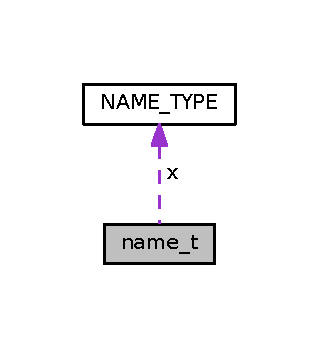
\includegraphics[width=153pt]{structname__t__coll__graph}
\end{center}
\end{figure}
\subsection*{Public Attributes}
\begin{DoxyCompactItemize}
\item 
\hyperlink{structNAME__TYPE}{N\+A\+M\+E\+\_\+\+T\+Y\+PE} \hyperlink{structname__t_aeef167ae3c011b675cd10f9e440ba4ff}{x}
\end{DoxyCompactItemize}


\subsection{Member Data Documentation}
\index{name\+\_\+t@{name\+\_\+t}!x@{x}}
\index{x@{x}!name\+\_\+t@{name\+\_\+t}}
\subsubsection[{\texorpdfstring{x}{x}}]{\setlength{\rightskip}{0pt plus 5cm}{\bf N\+A\+M\+E\+\_\+\+T\+Y\+PE} name\+\_\+t\+::x}\hypertarget{structname__t_aeef167ae3c011b675cd10f9e440ba4ff}{}\label{structname__t_aeef167ae3c011b675cd10f9e440ba4ff}


The documentation for this struct was generated from the following file\+:\begin{DoxyCompactItemize}
\item 
src/types/include/\hyperlink{general__types_8hpp}{general\+\_\+types.\+hpp}\end{DoxyCompactItemize}

\hypertarget{structNAME__TYPE}{}\section{N\+A\+M\+E\+\_\+\+T\+Y\+PE Struct Reference}
\label{structNAME__TYPE}\index{N\+A\+M\+E\+\_\+\+T\+Y\+PE@{N\+A\+M\+E\+\_\+\+T\+Y\+PE}}


{\ttfamily \#include $<$apex\+\_\+types.\+h$>$}

\subsection*{Public Attributes}
\begin{DoxyCompactItemize}
\item 
const char $\ast$ \hyperlink{structNAME__TYPE_ac5677dd8b326510aa1b29a3b43c0ead6}{x} \mbox{[}\hyperlink{apex__types_8h_ac74d8fef3c389eb3db8dd1681031d7bf}{M\+A\+X\+\_\+\+N\+A\+M\+E\+\_\+\+L\+E\+N\+G\+TH}\mbox{]}
\end{DoxyCompactItemize}


\subsection{Member Data Documentation}
\index{N\+A\+M\+E\+\_\+\+T\+Y\+PE@{N\+A\+M\+E\+\_\+\+T\+Y\+PE}!x@{x}}
\index{x@{x}!N\+A\+M\+E\+\_\+\+T\+Y\+PE@{N\+A\+M\+E\+\_\+\+T\+Y\+PE}}
\subsubsection[{\texorpdfstring{x}{x}}]{\setlength{\rightskip}{0pt plus 5cm}const char$\ast$ N\+A\+M\+E\+\_\+\+T\+Y\+P\+E\+::x\mbox{[}{\bf M\+A\+X\+\_\+\+N\+A\+M\+E\+\_\+\+L\+E\+N\+G\+TH}\mbox{]}}\hypertarget{structNAME__TYPE_ac5677dd8b326510aa1b29a3b43c0ead6}{}\label{structNAME__TYPE_ac5677dd8b326510aa1b29a3b43c0ead6}


The documentation for this struct was generated from the following file\+:\begin{DoxyCompactItemize}
\item 
src/libuser/apex/\hyperlink{apex__types_8h}{apex\+\_\+types.\+h}\end{DoxyCompactItemize}

\hypertarget{classPartition}{}\section{Partition Class Reference}
\label{classPartition}\index{Partition@{Partition}}


{\ttfamily \#include $<$partition.\+hpp$>$}

\subsection*{Public Member Functions}
\begin{DoxyCompactItemize}
\item 
\hyperlink{classPartition_aa8a055cfc129cee2a2ef024556fb6c0d}{Partition} ()
\item 
\hyperlink{classPartition_aa107f9e018df969f66596e35cef04aba}{Partition} (\hyperlink{general__types_8hpp_a824b78b06da8112c2772bc666a63638d}{identifier\+\_\+t} id, \hyperlink{apex__types_8h_ac081e44ca764e4d769f88a7f3bbc60de}{P\+R\+O\+C\+E\+S\+S\+O\+R\+\_\+\+C\+O\+R\+E\+\_\+\+I\+D\+\_\+\+T\+Y\+PE} affinity, \hyperlink{structname__t}{name\+\_\+t} name, \hyperlink{general__types_8hpp_a0edc3a86ddf4aa205c6882b61cd7b4e9}{dec\+Or\+Hex\+\_\+t} duration, \hyperlink{general__types_8hpp_a0edc3a86ddf4aa205c6882b61cd7b4e9}{dec\+Or\+Hex\+\_\+t} period, std\+::initializer\+\_\+list$<$ \hyperlink{classMemoryRegion}{Memory\+Region} $>$ mem, std\+::initializer\+\_\+list$<$ \hyperlink{classQueuingPort}{Queuing\+Port} $>$ queuing, std\+::initializer\+\_\+list$<$ \hyperlink{classSamplingPort}{Sampling\+Port} $>$ sampling)
\item 
\hyperlink{classPartition_ae7720ab349b46291bacc1a596dee2cd3}{Partition} (\hyperlink{general__types_8hpp_a824b78b06da8112c2772bc666a63638d}{identifier\+\_\+t} id, \hyperlink{apex__types_8h_ac081e44ca764e4d769f88a7f3bbc60de}{P\+R\+O\+C\+E\+S\+S\+O\+R\+\_\+\+C\+O\+R\+E\+\_\+\+I\+D\+\_\+\+T\+Y\+PE} affinity, \hyperlink{structname__t}{name\+\_\+t} name, \hyperlink{general__types_8hpp_a0edc3a86ddf4aa205c6882b61cd7b4e9}{dec\+Or\+Hex\+\_\+t} duration, \hyperlink{general__types_8hpp_a0edc3a86ddf4aa205c6882b61cd7b4e9}{dec\+Or\+Hex\+\_\+t} period, std\+::initializer\+\_\+list$<$ \hyperlink{classMemoryRegion}{Memory\+Region} $>$ mem, std\+::initializer\+\_\+list$<$ \hyperlink{classQueuingPort}{Queuing\+Port} $>$ queuing, std\+::initializer\+\_\+list$<$ \hyperlink{classSamplingPort}{Sampling\+Port} $>$ sampling, std\+::initializer\+\_\+list$<$ \hyperlink{classProcess}{Process} $>$ proc)
\item 
\hyperlink{classPartition_a7b73af2fd7f67503730f5c71c62fe6c6}{Partition} (const \hyperlink{classPartition}{Partition} \&rhs)
\item 
\hyperlink{classPartition}{Partition} \& \hyperlink{classPartition_a713dda6b4b83804b2a89acd80e1943c8}{operator=} (const \hyperlink{classPartition}{Partition} \&rhs)
\item 
const \hyperlink{general__types_8hpp_a824b78b06da8112c2772bc666a63638d}{identifier\+\_\+t} \& \hyperlink{classPartition_a9cc857400ee0e4f9ee8aa4b9a781c404}{get\+Partition\+Identifier} () const 
\item 
const \hyperlink{apex__types_8h_ac081e44ca764e4d769f88a7f3bbc60de}{P\+R\+O\+C\+E\+S\+S\+O\+R\+\_\+\+C\+O\+R\+E\+\_\+\+I\+D\+\_\+\+T\+Y\+PE} \& \hyperlink{classPartition_a4c2128f809210418d6c51b984a9eceac}{get\+Affinity} () const 
\item 
const \hyperlink{structname__t}{name\+\_\+t} \& \hyperlink{classPartition_a354db1a01962503fd33d2fd7aa52a46d}{get\+Partition\+Name} () const 
\item 
const \hyperlink{general__types_8hpp_a0edc3a86ddf4aa205c6882b61cd7b4e9}{dec\+Or\+Hex\+\_\+t} \& \hyperlink{classPartition_a018beb609fcd147efb7fd20594f6446d}{get\+Duration} () const 
\item 
const \hyperlink{general__types_8hpp_a0edc3a86ddf4aa205c6882b61cd7b4e9}{dec\+Or\+Hex\+\_\+t} \& \hyperlink{classPartition_af904def70aa07d2ba5b13d7cdd376c2c}{get\+Period} () const 
\item 
const std\+::vector$<$ \hyperlink{classMemoryRegion}{Memory\+Region} $>$ \& \hyperlink{classPartition_aa408f64e917a3aa805a3beb2d0b2669f}{get\+Memory\+Regions} () const 
\item 
const std\+::vector$<$ \hyperlink{classQueuingPort}{Queuing\+Port} $>$ \& \hyperlink{classPartition_a052021916099d1ca1dfeb44da62216df}{get\+Queue\+Ports} () const 
\item 
const std\+::vector$<$ \hyperlink{classSamplingPort}{Sampling\+Port} $>$ \& \hyperlink{classPartition_a04d5680e6be455ed8fcd96ce18ae1f79}{get\+Sample\+Ports} () const 
\item 
void \hyperlink{classPartition_affe5d93a0bfe4e8af9a3cdfc8bc80091}{set\+Mode} (\hyperlink{apex__partition_8h_a79d9616db80ce78328edcd1987aa90b1}{O\+P\+E\+R\+A\+T\+I\+N\+G\+\_\+\+M\+O\+D\+E\+\_\+\+T\+Y\+PE} mode)
\item 
const \hyperlink{apex__partition_8h_a79d9616db80ce78328edcd1987aa90b1}{O\+P\+E\+R\+A\+T\+I\+N\+G\+\_\+\+M\+O\+D\+E\+\_\+\+T\+Y\+PE} \& \hyperlink{classPartition_a2861314450a4ff0256d7b3e0b5640860}{get\+Mode} () const 
\item 
void \hyperlink{classPartition_aed0a52094368817b82384b6cb7ec73d6}{set\+Status} (\hyperlink{structPARTITION__STATUS__TYPE}{P\+A\+R\+T\+I\+T\+I\+O\+N\+\_\+\+S\+T\+A\+T\+U\+S\+\_\+\+T\+Y\+PE} status)
\item 
const \hyperlink{structPARTITION__STATUS__TYPE}{P\+A\+R\+T\+I\+T\+I\+O\+N\+\_\+\+S\+T\+A\+T\+U\+S\+\_\+\+T\+Y\+PE} \& \hyperlink{classPartition_ac2bcd024188150562d8f3c589254eb0d}{get\+Status} () const 
\item 
void \hyperlink{classPartition_af6cf1b68004cc5d8c0b01dd3b98af915}{add\+Process} (\hyperlink{classProcess}{Process} proc)
\item 
const std\+::vector$<$ \hyperlink{classProcess}{Process} $>$ \& \hyperlink{classPartition_a6b6da2b79e614c468c69c26def1f5394}{get\+Processes} () const 
\item 
void \hyperlink{classPartition_a1a5ced048aae9fabe24ffd61a1824151}{set\+Criticality} (\hyperlink{apex__partition_8h_a35bef4a19040ba19b0272682b87d200c}{C\+R\+I\+T\+I\+C\+A\+L\+I\+T\+Y\+\_\+\+T\+Y\+PE} criticality)
\item 
const \hyperlink{apex__partition_8h_a35bef4a19040ba19b0272682b87d200c}{C\+R\+I\+T\+I\+C\+A\+L\+I\+T\+Y\+\_\+\+T\+Y\+PE} \& \hyperlink{classPartition_a461e98f51321893eed11426720885c1e}{get\+Criticality} () const 
\item 
void \hyperlink{classPartition_a17d7fba34dd2fe6fb19985f0136b97ba}{set\+System\+Partition} (bool system\+Part)
\item 
const bool \& \hyperlink{classPartition_a409522daab48150242eba59a5f3f8b0d}{get\+System\+Partition} () const 
\item 
void \hyperlink{classPartition_a81513c0b6c3b94906ba87cadc46dcc7c}{set\+Entry\+Point} (\hyperlink{structname__t}{name\+\_\+t} entry)
\item 
const \hyperlink{structname__t}{name\+\_\+t} \& \hyperlink{classPartition_a8c56dbba844842a7e5dfb7ab387aed99}{get\+Entry\+Point} () const 
\end{DoxyCompactItemize}


\subsection{Constructor \& Destructor Documentation}
\index{Partition@{Partition}!Partition@{Partition}}
\index{Partition@{Partition}!Partition@{Partition}}
\subsubsection[{\texorpdfstring{Partition()}{Partition()}}]{\setlength{\rightskip}{0pt plus 5cm}Partition\+::\+Partition (
\begin{DoxyParamCaption}
{}
\end{DoxyParamCaption}
)\hspace{0.3cm}{\ttfamily [inline]}}\hypertarget{classPartition_aa8a055cfc129cee2a2ef024556fb6c0d}{}\label{classPartition_aa8a055cfc129cee2a2ef024556fb6c0d}
\index{Partition@{Partition}!Partition@{Partition}}
\index{Partition@{Partition}!Partition@{Partition}}
\subsubsection[{\texorpdfstring{Partition(identifier\+\_\+t id, P\+R\+O\+C\+E\+S\+S\+O\+R\+\_\+\+C\+O\+R\+E\+\_\+\+I\+D\+\_\+\+T\+Y\+P\+E affinity, name\+\_\+t name, dec\+Or\+Hex\+\_\+t duration, dec\+Or\+Hex\+\_\+t period, std\+::initializer\+\_\+list$<$ Memory\+Region $>$ mem, std\+::initializer\+\_\+list$<$ Queuing\+Port $>$ queuing, std\+::initializer\+\_\+list$<$ Sampling\+Port $>$ sampling)}{Partition(identifier_t id, PROCESSOR_CORE_ID_TYPE affinity, name_t name, decOrHex_t duration, decOrHex_t period, std::initializer_list< MemoryRegion > mem, std::initializer_list< QueuingPort > queuing, std::initializer_list< SamplingPort > sampling)}}]{\setlength{\rightskip}{0pt plus 5cm}Partition\+::\+Partition (
\begin{DoxyParamCaption}
\item[{{\bf identifier\+\_\+t}}]{id, }
\item[{{\bf P\+R\+O\+C\+E\+S\+S\+O\+R\+\_\+\+C\+O\+R\+E\+\_\+\+I\+D\+\_\+\+T\+Y\+PE}}]{affinity, }
\item[{{\bf name\+\_\+t}}]{name, }
\item[{{\bf dec\+Or\+Hex\+\_\+t}}]{duration, }
\item[{{\bf dec\+Or\+Hex\+\_\+t}}]{period, }
\item[{std\+::initializer\+\_\+list$<$ {\bf Memory\+Region} $>$}]{mem, }
\item[{std\+::initializer\+\_\+list$<$ {\bf Queuing\+Port} $>$}]{queuing, }
\item[{std\+::initializer\+\_\+list$<$ {\bf Sampling\+Port} $>$}]{sampling}
\end{DoxyParamCaption}
)\hspace{0.3cm}{\ttfamily [inline]}}\hypertarget{classPartition_aa107f9e018df969f66596e35cef04aba}{}\label{classPartition_aa107f9e018df969f66596e35cef04aba}
\index{Partition@{Partition}!Partition@{Partition}}
\index{Partition@{Partition}!Partition@{Partition}}
\subsubsection[{\texorpdfstring{Partition(identifier\+\_\+t id, P\+R\+O\+C\+E\+S\+S\+O\+R\+\_\+\+C\+O\+R\+E\+\_\+\+I\+D\+\_\+\+T\+Y\+P\+E affinity, name\+\_\+t name, dec\+Or\+Hex\+\_\+t duration, dec\+Or\+Hex\+\_\+t period, std\+::initializer\+\_\+list$<$ Memory\+Region $>$ mem, std\+::initializer\+\_\+list$<$ Queuing\+Port $>$ queuing, std\+::initializer\+\_\+list$<$ Sampling\+Port $>$ sampling, std\+::initializer\+\_\+list$<$ Process $>$ proc)}{Partition(identifier_t id, PROCESSOR_CORE_ID_TYPE affinity, name_t name, decOrHex_t duration, decOrHex_t period, std::initializer_list< MemoryRegion > mem, std::initializer_list< QueuingPort > queuing, std::initializer_list< SamplingPort > sampling, std::initializer_list< Process > proc)}}]{\setlength{\rightskip}{0pt plus 5cm}Partition\+::\+Partition (
\begin{DoxyParamCaption}
\item[{{\bf identifier\+\_\+t}}]{id, }
\item[{{\bf P\+R\+O\+C\+E\+S\+S\+O\+R\+\_\+\+C\+O\+R\+E\+\_\+\+I\+D\+\_\+\+T\+Y\+PE}}]{affinity, }
\item[{{\bf name\+\_\+t}}]{name, }
\item[{{\bf dec\+Or\+Hex\+\_\+t}}]{duration, }
\item[{{\bf dec\+Or\+Hex\+\_\+t}}]{period, }
\item[{std\+::initializer\+\_\+list$<$ {\bf Memory\+Region} $>$}]{mem, }
\item[{std\+::initializer\+\_\+list$<$ {\bf Queuing\+Port} $>$}]{queuing, }
\item[{std\+::initializer\+\_\+list$<$ {\bf Sampling\+Port} $>$}]{sampling, }
\item[{std\+::initializer\+\_\+list$<$ {\bf Process} $>$}]{proc}
\end{DoxyParamCaption}
)\hspace{0.3cm}{\ttfamily [inline]}}\hypertarget{classPartition_ae7720ab349b46291bacc1a596dee2cd3}{}\label{classPartition_ae7720ab349b46291bacc1a596dee2cd3}
\index{Partition@{Partition}!Partition@{Partition}}
\index{Partition@{Partition}!Partition@{Partition}}
\subsubsection[{\texorpdfstring{Partition(const Partition \&rhs)}{Partition(const Partition &rhs)}}]{\setlength{\rightskip}{0pt plus 5cm}Partition\+::\+Partition (
\begin{DoxyParamCaption}
\item[{const {\bf Partition} \&}]{rhs}
\end{DoxyParamCaption}
)\hspace{0.3cm}{\ttfamily [inline]}}\hypertarget{classPartition_a7b73af2fd7f67503730f5c71c62fe6c6}{}\label{classPartition_a7b73af2fd7f67503730f5c71c62fe6c6}


\subsection{Member Function Documentation}
\index{Partition@{Partition}!add\+Process@{add\+Process}}
\index{add\+Process@{add\+Process}!Partition@{Partition}}
\subsubsection[{\texorpdfstring{add\+Process(\+Process proc)}{addProcess(Process proc)}}]{\setlength{\rightskip}{0pt plus 5cm}void Partition\+::add\+Process (
\begin{DoxyParamCaption}
\item[{{\bf Process}}]{proc}
\end{DoxyParamCaption}
)}\hypertarget{classPartition_af6cf1b68004cc5d8c0b01dd3b98af915}{}\label{classPartition_af6cf1b68004cc5d8c0b01dd3b98af915}
\index{Partition@{Partition}!get\+Affinity@{get\+Affinity}}
\index{get\+Affinity@{get\+Affinity}!Partition@{Partition}}
\subsubsection[{\texorpdfstring{get\+Affinity() const }{getAffinity() const }}]{\setlength{\rightskip}{0pt plus 5cm}const {\bf P\+R\+O\+C\+E\+S\+S\+O\+R\+\_\+\+C\+O\+R\+E\+\_\+\+I\+D\+\_\+\+T\+Y\+PE} \& Partition\+::get\+Affinity (
\begin{DoxyParamCaption}
{}
\end{DoxyParamCaption}
) const}\hypertarget{classPartition_a4c2128f809210418d6c51b984a9eceac}{}\label{classPartition_a4c2128f809210418d6c51b984a9eceac}
\index{Partition@{Partition}!get\+Criticality@{get\+Criticality}}
\index{get\+Criticality@{get\+Criticality}!Partition@{Partition}}
\subsubsection[{\texorpdfstring{get\+Criticality() const }{getCriticality() const }}]{\setlength{\rightskip}{0pt plus 5cm}const {\bf C\+R\+I\+T\+I\+C\+A\+L\+I\+T\+Y\+\_\+\+T\+Y\+PE} \& Partition\+::get\+Criticality (
\begin{DoxyParamCaption}
{}
\end{DoxyParamCaption}
) const}\hypertarget{classPartition_a461e98f51321893eed11426720885c1e}{}\label{classPartition_a461e98f51321893eed11426720885c1e}
\index{Partition@{Partition}!get\+Duration@{get\+Duration}}
\index{get\+Duration@{get\+Duration}!Partition@{Partition}}
\subsubsection[{\texorpdfstring{get\+Duration() const }{getDuration() const }}]{\setlength{\rightskip}{0pt plus 5cm}const {\bf dec\+Or\+Hex\+\_\+t} \& Partition\+::get\+Duration (
\begin{DoxyParamCaption}
{}
\end{DoxyParamCaption}
) const}\hypertarget{classPartition_a018beb609fcd147efb7fd20594f6446d}{}\label{classPartition_a018beb609fcd147efb7fd20594f6446d}
\index{Partition@{Partition}!get\+Entry\+Point@{get\+Entry\+Point}}
\index{get\+Entry\+Point@{get\+Entry\+Point}!Partition@{Partition}}
\subsubsection[{\texorpdfstring{get\+Entry\+Point() const }{getEntryPoint() const }}]{\setlength{\rightskip}{0pt plus 5cm}const {\bf name\+\_\+t} \& Partition\+::get\+Entry\+Point (
\begin{DoxyParamCaption}
{}
\end{DoxyParamCaption}
) const}\hypertarget{classPartition_a8c56dbba844842a7e5dfb7ab387aed99}{}\label{classPartition_a8c56dbba844842a7e5dfb7ab387aed99}
\index{Partition@{Partition}!get\+Memory\+Regions@{get\+Memory\+Regions}}
\index{get\+Memory\+Regions@{get\+Memory\+Regions}!Partition@{Partition}}
\subsubsection[{\texorpdfstring{get\+Memory\+Regions() const }{getMemoryRegions() const }}]{\setlength{\rightskip}{0pt plus 5cm}const std\+::vector$<$ {\bf Memory\+Region} $>$ \& Partition\+::get\+Memory\+Regions (
\begin{DoxyParamCaption}
{}
\end{DoxyParamCaption}
) const}\hypertarget{classPartition_aa408f64e917a3aa805a3beb2d0b2669f}{}\label{classPartition_aa408f64e917a3aa805a3beb2d0b2669f}
\index{Partition@{Partition}!get\+Mode@{get\+Mode}}
\index{get\+Mode@{get\+Mode}!Partition@{Partition}}
\subsubsection[{\texorpdfstring{get\+Mode() const }{getMode() const }}]{\setlength{\rightskip}{0pt plus 5cm}const {\bf O\+P\+E\+R\+A\+T\+I\+N\+G\+\_\+\+M\+O\+D\+E\+\_\+\+T\+Y\+PE} \& Partition\+::get\+Mode (
\begin{DoxyParamCaption}
{}
\end{DoxyParamCaption}
) const}\hypertarget{classPartition_a2861314450a4ff0256d7b3e0b5640860}{}\label{classPartition_a2861314450a4ff0256d7b3e0b5640860}
\index{Partition@{Partition}!get\+Partition\+Identifier@{get\+Partition\+Identifier}}
\index{get\+Partition\+Identifier@{get\+Partition\+Identifier}!Partition@{Partition}}
\subsubsection[{\texorpdfstring{get\+Partition\+Identifier() const }{getPartitionIdentifier() const }}]{\setlength{\rightskip}{0pt plus 5cm}const {\bf identifier\+\_\+t} \& Partition\+::get\+Partition\+Identifier (
\begin{DoxyParamCaption}
{}
\end{DoxyParamCaption}
) const}\hypertarget{classPartition_a9cc857400ee0e4f9ee8aa4b9a781c404}{}\label{classPartition_a9cc857400ee0e4f9ee8aa4b9a781c404}
\index{Partition@{Partition}!get\+Partition\+Name@{get\+Partition\+Name}}
\index{get\+Partition\+Name@{get\+Partition\+Name}!Partition@{Partition}}
\subsubsection[{\texorpdfstring{get\+Partition\+Name() const }{getPartitionName() const }}]{\setlength{\rightskip}{0pt plus 5cm}const {\bf name\+\_\+t} \& Partition\+::get\+Partition\+Name (
\begin{DoxyParamCaption}
{}
\end{DoxyParamCaption}
) const}\hypertarget{classPartition_a354db1a01962503fd33d2fd7aa52a46d}{}\label{classPartition_a354db1a01962503fd33d2fd7aa52a46d}
\index{Partition@{Partition}!get\+Period@{get\+Period}}
\index{get\+Period@{get\+Period}!Partition@{Partition}}
\subsubsection[{\texorpdfstring{get\+Period() const }{getPeriod() const }}]{\setlength{\rightskip}{0pt plus 5cm}const {\bf dec\+Or\+Hex\+\_\+t} \& Partition\+::get\+Period (
\begin{DoxyParamCaption}
{}
\end{DoxyParamCaption}
) const}\hypertarget{classPartition_af904def70aa07d2ba5b13d7cdd376c2c}{}\label{classPartition_af904def70aa07d2ba5b13d7cdd376c2c}
\index{Partition@{Partition}!get\+Processes@{get\+Processes}}
\index{get\+Processes@{get\+Processes}!Partition@{Partition}}
\subsubsection[{\texorpdfstring{get\+Processes() const }{getProcesses() const }}]{\setlength{\rightskip}{0pt plus 5cm}const std\+::vector$<$ {\bf Process} $>$ \& Partition\+::get\+Processes (
\begin{DoxyParamCaption}
{}
\end{DoxyParamCaption}
) const}\hypertarget{classPartition_a6b6da2b79e614c468c69c26def1f5394}{}\label{classPartition_a6b6da2b79e614c468c69c26def1f5394}
\index{Partition@{Partition}!get\+Queue\+Ports@{get\+Queue\+Ports}}
\index{get\+Queue\+Ports@{get\+Queue\+Ports}!Partition@{Partition}}
\subsubsection[{\texorpdfstring{get\+Queue\+Ports() const }{getQueuePorts() const }}]{\setlength{\rightskip}{0pt plus 5cm}const std\+::vector$<$ {\bf Queuing\+Port} $>$ \& Partition\+::get\+Queue\+Ports (
\begin{DoxyParamCaption}
{}
\end{DoxyParamCaption}
) const}\hypertarget{classPartition_a052021916099d1ca1dfeb44da62216df}{}\label{classPartition_a052021916099d1ca1dfeb44da62216df}
\index{Partition@{Partition}!get\+Sample\+Ports@{get\+Sample\+Ports}}
\index{get\+Sample\+Ports@{get\+Sample\+Ports}!Partition@{Partition}}
\subsubsection[{\texorpdfstring{get\+Sample\+Ports() const }{getSamplePorts() const }}]{\setlength{\rightskip}{0pt plus 5cm}const std\+::vector$<$ {\bf Sampling\+Port} $>$ \& Partition\+::get\+Sample\+Ports (
\begin{DoxyParamCaption}
{}
\end{DoxyParamCaption}
) const}\hypertarget{classPartition_a04d5680e6be455ed8fcd96ce18ae1f79}{}\label{classPartition_a04d5680e6be455ed8fcd96ce18ae1f79}
\index{Partition@{Partition}!get\+Status@{get\+Status}}
\index{get\+Status@{get\+Status}!Partition@{Partition}}
\subsubsection[{\texorpdfstring{get\+Status() const }{getStatus() const }}]{\setlength{\rightskip}{0pt plus 5cm}const {\bf P\+A\+R\+T\+I\+T\+I\+O\+N\+\_\+\+S\+T\+A\+T\+U\+S\+\_\+\+T\+Y\+PE} \& Partition\+::get\+Status (
\begin{DoxyParamCaption}
{}
\end{DoxyParamCaption}
) const}\hypertarget{classPartition_ac2bcd024188150562d8f3c589254eb0d}{}\label{classPartition_ac2bcd024188150562d8f3c589254eb0d}
\index{Partition@{Partition}!get\+System\+Partition@{get\+System\+Partition}}
\index{get\+System\+Partition@{get\+System\+Partition}!Partition@{Partition}}
\subsubsection[{\texorpdfstring{get\+System\+Partition() const }{getSystemPartition() const }}]{\setlength{\rightskip}{0pt plus 5cm}const bool \& Partition\+::get\+System\+Partition (
\begin{DoxyParamCaption}
{}
\end{DoxyParamCaption}
) const}\hypertarget{classPartition_a409522daab48150242eba59a5f3f8b0d}{}\label{classPartition_a409522daab48150242eba59a5f3f8b0d}
\index{Partition@{Partition}!operator=@{operator=}}
\index{operator=@{operator=}!Partition@{Partition}}
\subsubsection[{\texorpdfstring{operator=(const Partition \&rhs)}{operator=(const Partition &rhs)}}]{\setlength{\rightskip}{0pt plus 5cm}{\bf Partition} \& Partition\+::operator= (
\begin{DoxyParamCaption}
\item[{const {\bf Partition} \&}]{rhs}
\end{DoxyParamCaption}
)}\hypertarget{classPartition_a713dda6b4b83804b2a89acd80e1943c8}{}\label{classPartition_a713dda6b4b83804b2a89acd80e1943c8}
\index{Partition@{Partition}!set\+Criticality@{set\+Criticality}}
\index{set\+Criticality@{set\+Criticality}!Partition@{Partition}}
\subsubsection[{\texorpdfstring{set\+Criticality(\+C\+R\+I\+T\+I\+C\+A\+L\+I\+T\+Y\+\_\+\+T\+Y\+P\+E criticality)}{setCriticality(CRITICALITY_TYPE criticality)}}]{\setlength{\rightskip}{0pt plus 5cm}void Partition\+::set\+Criticality (
\begin{DoxyParamCaption}
\item[{{\bf C\+R\+I\+T\+I\+C\+A\+L\+I\+T\+Y\+\_\+\+T\+Y\+PE}}]{criticality}
\end{DoxyParamCaption}
)}\hypertarget{classPartition_a1a5ced048aae9fabe24ffd61a1824151}{}\label{classPartition_a1a5ced048aae9fabe24ffd61a1824151}
\index{Partition@{Partition}!set\+Entry\+Point@{set\+Entry\+Point}}
\index{set\+Entry\+Point@{set\+Entry\+Point}!Partition@{Partition}}
\subsubsection[{\texorpdfstring{set\+Entry\+Point(name\+\_\+t entry)}{setEntryPoint(name_t entry)}}]{\setlength{\rightskip}{0pt plus 5cm}void Partition\+::set\+Entry\+Point (
\begin{DoxyParamCaption}
\item[{{\bf name\+\_\+t}}]{entry}
\end{DoxyParamCaption}
)}\hypertarget{classPartition_a81513c0b6c3b94906ba87cadc46dcc7c}{}\label{classPartition_a81513c0b6c3b94906ba87cadc46dcc7c}
\index{Partition@{Partition}!set\+Mode@{set\+Mode}}
\index{set\+Mode@{set\+Mode}!Partition@{Partition}}
\subsubsection[{\texorpdfstring{set\+Mode(\+O\+P\+E\+R\+A\+T\+I\+N\+G\+\_\+\+M\+O\+D\+E\+\_\+\+T\+Y\+P\+E mode)}{setMode(OPERATING_MODE_TYPE mode)}}]{\setlength{\rightskip}{0pt plus 5cm}void Partition\+::set\+Mode (
\begin{DoxyParamCaption}
\item[{{\bf O\+P\+E\+R\+A\+T\+I\+N\+G\+\_\+\+M\+O\+D\+E\+\_\+\+T\+Y\+PE}}]{mode}
\end{DoxyParamCaption}
)}\hypertarget{classPartition_affe5d93a0bfe4e8af9a3cdfc8bc80091}{}\label{classPartition_affe5d93a0bfe4e8af9a3cdfc8bc80091}
\index{Partition@{Partition}!set\+Status@{set\+Status}}
\index{set\+Status@{set\+Status}!Partition@{Partition}}
\subsubsection[{\texorpdfstring{set\+Status(\+P\+A\+R\+T\+I\+T\+I\+O\+N\+\_\+\+S\+T\+A\+T\+U\+S\+\_\+\+T\+Y\+P\+E status)}{setStatus(PARTITION_STATUS_TYPE status)}}]{\setlength{\rightskip}{0pt plus 5cm}void Partition\+::set\+Status (
\begin{DoxyParamCaption}
\item[{{\bf P\+A\+R\+T\+I\+T\+I\+O\+N\+\_\+\+S\+T\+A\+T\+U\+S\+\_\+\+T\+Y\+PE}}]{status}
\end{DoxyParamCaption}
)}\hypertarget{classPartition_aed0a52094368817b82384b6cb7ec73d6}{}\label{classPartition_aed0a52094368817b82384b6cb7ec73d6}
\index{Partition@{Partition}!set\+System\+Partition@{set\+System\+Partition}}
\index{set\+System\+Partition@{set\+System\+Partition}!Partition@{Partition}}
\subsubsection[{\texorpdfstring{set\+System\+Partition(bool system\+Part)}{setSystemPartition(bool systemPart)}}]{\setlength{\rightskip}{0pt plus 5cm}void Partition\+::set\+System\+Partition (
\begin{DoxyParamCaption}
\item[{bool}]{system\+Part}
\end{DoxyParamCaption}
)}\hypertarget{classPartition_a17d7fba34dd2fe6fb19985f0136b97ba}{}\label{classPartition_a17d7fba34dd2fe6fb19985f0136b97ba}


The documentation for this class was generated from the following files\+:\begin{DoxyCompactItemize}
\item 
src/types/include/\hyperlink{partition_8hpp}{partition.\+hpp}\item 
src/types/src/\hyperlink{partition_8cpp}{partition.\+cpp}\end{DoxyCompactItemize}

\hypertarget{structPARTITION__STATUS__TYPE}{}\section{P\+A\+R\+T\+I\+T\+I\+O\+N\+\_\+\+S\+T\+A\+T\+U\+S\+\_\+\+T\+Y\+PE Struct Reference}
\label{structPARTITION__STATUS__TYPE}\index{P\+A\+R\+T\+I\+T\+I\+O\+N\+\_\+\+S\+T\+A\+T\+U\+S\+\_\+\+T\+Y\+PE@{P\+A\+R\+T\+I\+T\+I\+O\+N\+\_\+\+S\+T\+A\+T\+U\+S\+\_\+\+T\+Y\+PE}}


{\ttfamily \#include $<$apex\+\_\+partition.\+h$>$}

\subsection*{Public Attributes}
\begin{DoxyCompactItemize}
\item 
\hyperlink{apex__types_8h_a78cd52c2621ddf2eda68fcd4bedbc1a7}{S\+Y\+S\+T\+E\+M\+\_\+\+T\+I\+M\+E\+\_\+\+T\+Y\+PE} \hyperlink{structPARTITION__STATUS__TYPE_af7b3d2efeee84266bb2272989468a77b}{P\+E\+R\+I\+OD}
\item 
\hyperlink{apex__types_8h_a78cd52c2621ddf2eda68fcd4bedbc1a7}{S\+Y\+S\+T\+E\+M\+\_\+\+T\+I\+M\+E\+\_\+\+T\+Y\+PE} \hyperlink{structPARTITION__STATUS__TYPE_add054a9d2ba7b24f4d891aefb7ad129b}{D\+U\+R\+A\+T\+I\+ON}
\item 
\hyperlink{apex__partition_8h_a98710ee510022d5d100c8f2d320efad7}{P\+A\+R\+T\+I\+T\+I\+O\+N\+\_\+\+I\+D\+\_\+\+T\+Y\+PE} \hyperlink{structPARTITION__STATUS__TYPE_a7a769c63fafb1db12e997539dbbf92ae}{I\+D\+E\+N\+T\+I\+F\+I\+ER}
\item 
\hyperlink{apex__process_8h_a45e0a7a5bf30c61fe6a5fe1ed96f27d2}{L\+O\+C\+K\+\_\+\+L\+E\+V\+E\+L\+\_\+\+T\+Y\+PE} \hyperlink{structPARTITION__STATUS__TYPE_a7897783426caa52ad5015696c41111c7}{L\+O\+C\+K\+\_\+\+L\+E\+V\+EL}
\item 
\hyperlink{apex__partition_8h_a79d9616db80ce78328edcd1987aa90b1}{O\+P\+E\+R\+A\+T\+I\+N\+G\+\_\+\+M\+O\+D\+E\+\_\+\+T\+Y\+PE} \hyperlink{structPARTITION__STATUS__TYPE_a11ddb9ecc1f3a00638bb282d442f4960}{O\+P\+E\+R\+A\+T\+I\+N\+G\+\_\+\+M\+O\+DE}
\item 
\hyperlink{apex__partition_8h_afefc0c2dc013745df97678ba67354324}{S\+T\+A\+R\+T\+\_\+\+C\+O\+N\+D\+I\+T\+I\+O\+N\+\_\+\+T\+Y\+PE} \hyperlink{structPARTITION__STATUS__TYPE_ac235ddfbaadeeffbe6a65f0f2fea69a6}{S\+T\+A\+R\+T\+\_\+\+C\+O\+N\+D\+I\+T\+I\+ON}
\item 
\hyperlink{apex__partition_8h_a010e5f5601385be74052b2c419491e28}{N\+U\+M\+\_\+\+C\+O\+R\+E\+S\+\_\+\+T\+Y\+PE} \hyperlink{structPARTITION__STATUS__TYPE_a811192806118ead344b259aa17b4e91f}{N\+U\+M\+\_\+\+A\+S\+S\+I\+G\+N\+E\+D\+\_\+\+C\+O\+R\+ES}
\end{DoxyCompactItemize}


\subsection{Member Data Documentation}
\index{P\+A\+R\+T\+I\+T\+I\+O\+N\+\_\+\+S\+T\+A\+T\+U\+S\+\_\+\+T\+Y\+PE@{P\+A\+R\+T\+I\+T\+I\+O\+N\+\_\+\+S\+T\+A\+T\+U\+S\+\_\+\+T\+Y\+PE}!D\+U\+R\+A\+T\+I\+ON@{D\+U\+R\+A\+T\+I\+ON}}
\index{D\+U\+R\+A\+T\+I\+ON@{D\+U\+R\+A\+T\+I\+ON}!P\+A\+R\+T\+I\+T\+I\+O\+N\+\_\+\+S\+T\+A\+T\+U\+S\+\_\+\+T\+Y\+PE@{P\+A\+R\+T\+I\+T\+I\+O\+N\+\_\+\+S\+T\+A\+T\+U\+S\+\_\+\+T\+Y\+PE}}
\subsubsection[{\texorpdfstring{D\+U\+R\+A\+T\+I\+ON}{DURATION}}]{\setlength{\rightskip}{0pt plus 5cm}{\bf S\+Y\+S\+T\+E\+M\+\_\+\+T\+I\+M\+E\+\_\+\+T\+Y\+PE} P\+A\+R\+T\+I\+T\+I\+O\+N\+\_\+\+S\+T\+A\+T\+U\+S\+\_\+\+T\+Y\+P\+E\+::\+D\+U\+R\+A\+T\+I\+ON}\hypertarget{structPARTITION__STATUS__TYPE_add054a9d2ba7b24f4d891aefb7ad129b}{}\label{structPARTITION__STATUS__TYPE_add054a9d2ba7b24f4d891aefb7ad129b}
\index{P\+A\+R\+T\+I\+T\+I\+O\+N\+\_\+\+S\+T\+A\+T\+U\+S\+\_\+\+T\+Y\+PE@{P\+A\+R\+T\+I\+T\+I\+O\+N\+\_\+\+S\+T\+A\+T\+U\+S\+\_\+\+T\+Y\+PE}!I\+D\+E\+N\+T\+I\+F\+I\+ER@{I\+D\+E\+N\+T\+I\+F\+I\+ER}}
\index{I\+D\+E\+N\+T\+I\+F\+I\+ER@{I\+D\+E\+N\+T\+I\+F\+I\+ER}!P\+A\+R\+T\+I\+T\+I\+O\+N\+\_\+\+S\+T\+A\+T\+U\+S\+\_\+\+T\+Y\+PE@{P\+A\+R\+T\+I\+T\+I\+O\+N\+\_\+\+S\+T\+A\+T\+U\+S\+\_\+\+T\+Y\+PE}}
\subsubsection[{\texorpdfstring{I\+D\+E\+N\+T\+I\+F\+I\+ER}{IDENTIFIER}}]{\setlength{\rightskip}{0pt plus 5cm}{\bf P\+A\+R\+T\+I\+T\+I\+O\+N\+\_\+\+I\+D\+\_\+\+T\+Y\+PE} P\+A\+R\+T\+I\+T\+I\+O\+N\+\_\+\+S\+T\+A\+T\+U\+S\+\_\+\+T\+Y\+P\+E\+::\+I\+D\+E\+N\+T\+I\+F\+I\+ER}\hypertarget{structPARTITION__STATUS__TYPE_a7a769c63fafb1db12e997539dbbf92ae}{}\label{structPARTITION__STATUS__TYPE_a7a769c63fafb1db12e997539dbbf92ae}
\index{P\+A\+R\+T\+I\+T\+I\+O\+N\+\_\+\+S\+T\+A\+T\+U\+S\+\_\+\+T\+Y\+PE@{P\+A\+R\+T\+I\+T\+I\+O\+N\+\_\+\+S\+T\+A\+T\+U\+S\+\_\+\+T\+Y\+PE}!L\+O\+C\+K\+\_\+\+L\+E\+V\+EL@{L\+O\+C\+K\+\_\+\+L\+E\+V\+EL}}
\index{L\+O\+C\+K\+\_\+\+L\+E\+V\+EL@{L\+O\+C\+K\+\_\+\+L\+E\+V\+EL}!P\+A\+R\+T\+I\+T\+I\+O\+N\+\_\+\+S\+T\+A\+T\+U\+S\+\_\+\+T\+Y\+PE@{P\+A\+R\+T\+I\+T\+I\+O\+N\+\_\+\+S\+T\+A\+T\+U\+S\+\_\+\+T\+Y\+PE}}
\subsubsection[{\texorpdfstring{L\+O\+C\+K\+\_\+\+L\+E\+V\+EL}{LOCK_LEVEL}}]{\setlength{\rightskip}{0pt plus 5cm}{\bf L\+O\+C\+K\+\_\+\+L\+E\+V\+E\+L\+\_\+\+T\+Y\+PE} P\+A\+R\+T\+I\+T\+I\+O\+N\+\_\+\+S\+T\+A\+T\+U\+S\+\_\+\+T\+Y\+P\+E\+::\+L\+O\+C\+K\+\_\+\+L\+E\+V\+EL}\hypertarget{structPARTITION__STATUS__TYPE_a7897783426caa52ad5015696c41111c7}{}\label{structPARTITION__STATUS__TYPE_a7897783426caa52ad5015696c41111c7}
\index{P\+A\+R\+T\+I\+T\+I\+O\+N\+\_\+\+S\+T\+A\+T\+U\+S\+\_\+\+T\+Y\+PE@{P\+A\+R\+T\+I\+T\+I\+O\+N\+\_\+\+S\+T\+A\+T\+U\+S\+\_\+\+T\+Y\+PE}!N\+U\+M\+\_\+\+A\+S\+S\+I\+G\+N\+E\+D\+\_\+\+C\+O\+R\+ES@{N\+U\+M\+\_\+\+A\+S\+S\+I\+G\+N\+E\+D\+\_\+\+C\+O\+R\+ES}}
\index{N\+U\+M\+\_\+\+A\+S\+S\+I\+G\+N\+E\+D\+\_\+\+C\+O\+R\+ES@{N\+U\+M\+\_\+\+A\+S\+S\+I\+G\+N\+E\+D\+\_\+\+C\+O\+R\+ES}!P\+A\+R\+T\+I\+T\+I\+O\+N\+\_\+\+S\+T\+A\+T\+U\+S\+\_\+\+T\+Y\+PE@{P\+A\+R\+T\+I\+T\+I\+O\+N\+\_\+\+S\+T\+A\+T\+U\+S\+\_\+\+T\+Y\+PE}}
\subsubsection[{\texorpdfstring{N\+U\+M\+\_\+\+A\+S\+S\+I\+G\+N\+E\+D\+\_\+\+C\+O\+R\+ES}{NUM_ASSIGNED_CORES}}]{\setlength{\rightskip}{0pt plus 5cm}{\bf N\+U\+M\+\_\+\+C\+O\+R\+E\+S\+\_\+\+T\+Y\+PE} P\+A\+R\+T\+I\+T\+I\+O\+N\+\_\+\+S\+T\+A\+T\+U\+S\+\_\+\+T\+Y\+P\+E\+::\+N\+U\+M\+\_\+\+A\+S\+S\+I\+G\+N\+E\+D\+\_\+\+C\+O\+R\+ES}\hypertarget{structPARTITION__STATUS__TYPE_a811192806118ead344b259aa17b4e91f}{}\label{structPARTITION__STATUS__TYPE_a811192806118ead344b259aa17b4e91f}
\index{P\+A\+R\+T\+I\+T\+I\+O\+N\+\_\+\+S\+T\+A\+T\+U\+S\+\_\+\+T\+Y\+PE@{P\+A\+R\+T\+I\+T\+I\+O\+N\+\_\+\+S\+T\+A\+T\+U\+S\+\_\+\+T\+Y\+PE}!O\+P\+E\+R\+A\+T\+I\+N\+G\+\_\+\+M\+O\+DE@{O\+P\+E\+R\+A\+T\+I\+N\+G\+\_\+\+M\+O\+DE}}
\index{O\+P\+E\+R\+A\+T\+I\+N\+G\+\_\+\+M\+O\+DE@{O\+P\+E\+R\+A\+T\+I\+N\+G\+\_\+\+M\+O\+DE}!P\+A\+R\+T\+I\+T\+I\+O\+N\+\_\+\+S\+T\+A\+T\+U\+S\+\_\+\+T\+Y\+PE@{P\+A\+R\+T\+I\+T\+I\+O\+N\+\_\+\+S\+T\+A\+T\+U\+S\+\_\+\+T\+Y\+PE}}
\subsubsection[{\texorpdfstring{O\+P\+E\+R\+A\+T\+I\+N\+G\+\_\+\+M\+O\+DE}{OPERATING_MODE}}]{\setlength{\rightskip}{0pt plus 5cm}{\bf O\+P\+E\+R\+A\+T\+I\+N\+G\+\_\+\+M\+O\+D\+E\+\_\+\+T\+Y\+PE} P\+A\+R\+T\+I\+T\+I\+O\+N\+\_\+\+S\+T\+A\+T\+U\+S\+\_\+\+T\+Y\+P\+E\+::\+O\+P\+E\+R\+A\+T\+I\+N\+G\+\_\+\+M\+O\+DE}\hypertarget{structPARTITION__STATUS__TYPE_a11ddb9ecc1f3a00638bb282d442f4960}{}\label{structPARTITION__STATUS__TYPE_a11ddb9ecc1f3a00638bb282d442f4960}
\index{P\+A\+R\+T\+I\+T\+I\+O\+N\+\_\+\+S\+T\+A\+T\+U\+S\+\_\+\+T\+Y\+PE@{P\+A\+R\+T\+I\+T\+I\+O\+N\+\_\+\+S\+T\+A\+T\+U\+S\+\_\+\+T\+Y\+PE}!P\+E\+R\+I\+OD@{P\+E\+R\+I\+OD}}
\index{P\+E\+R\+I\+OD@{P\+E\+R\+I\+OD}!P\+A\+R\+T\+I\+T\+I\+O\+N\+\_\+\+S\+T\+A\+T\+U\+S\+\_\+\+T\+Y\+PE@{P\+A\+R\+T\+I\+T\+I\+O\+N\+\_\+\+S\+T\+A\+T\+U\+S\+\_\+\+T\+Y\+PE}}
\subsubsection[{\texorpdfstring{P\+E\+R\+I\+OD}{PERIOD}}]{\setlength{\rightskip}{0pt plus 5cm}{\bf S\+Y\+S\+T\+E\+M\+\_\+\+T\+I\+M\+E\+\_\+\+T\+Y\+PE} P\+A\+R\+T\+I\+T\+I\+O\+N\+\_\+\+S\+T\+A\+T\+U\+S\+\_\+\+T\+Y\+P\+E\+::\+P\+E\+R\+I\+OD}\hypertarget{structPARTITION__STATUS__TYPE_af7b3d2efeee84266bb2272989468a77b}{}\label{structPARTITION__STATUS__TYPE_af7b3d2efeee84266bb2272989468a77b}
\index{P\+A\+R\+T\+I\+T\+I\+O\+N\+\_\+\+S\+T\+A\+T\+U\+S\+\_\+\+T\+Y\+PE@{P\+A\+R\+T\+I\+T\+I\+O\+N\+\_\+\+S\+T\+A\+T\+U\+S\+\_\+\+T\+Y\+PE}!S\+T\+A\+R\+T\+\_\+\+C\+O\+N\+D\+I\+T\+I\+ON@{S\+T\+A\+R\+T\+\_\+\+C\+O\+N\+D\+I\+T\+I\+ON}}
\index{S\+T\+A\+R\+T\+\_\+\+C\+O\+N\+D\+I\+T\+I\+ON@{S\+T\+A\+R\+T\+\_\+\+C\+O\+N\+D\+I\+T\+I\+ON}!P\+A\+R\+T\+I\+T\+I\+O\+N\+\_\+\+S\+T\+A\+T\+U\+S\+\_\+\+T\+Y\+PE@{P\+A\+R\+T\+I\+T\+I\+O\+N\+\_\+\+S\+T\+A\+T\+U\+S\+\_\+\+T\+Y\+PE}}
\subsubsection[{\texorpdfstring{S\+T\+A\+R\+T\+\_\+\+C\+O\+N\+D\+I\+T\+I\+ON}{START_CONDITION}}]{\setlength{\rightskip}{0pt plus 5cm}{\bf S\+T\+A\+R\+T\+\_\+\+C\+O\+N\+D\+I\+T\+I\+O\+N\+\_\+\+T\+Y\+PE} P\+A\+R\+T\+I\+T\+I\+O\+N\+\_\+\+S\+T\+A\+T\+U\+S\+\_\+\+T\+Y\+P\+E\+::\+S\+T\+A\+R\+T\+\_\+\+C\+O\+N\+D\+I\+T\+I\+ON}\hypertarget{structPARTITION__STATUS__TYPE_ac235ddfbaadeeffbe6a65f0f2fea69a6}{}\label{structPARTITION__STATUS__TYPE_ac235ddfbaadeeffbe6a65f0f2fea69a6}


The documentation for this struct was generated from the following file\+:\begin{DoxyCompactItemize}
\item 
src/libuser/apex/\hyperlink{apex__partition_8h}{apex\+\_\+partition.\+h}\end{DoxyCompactItemize}

\hypertarget{classPartitionErrorAction}{}\section{Partition\+Error\+Action Class Reference}
\label{classPartitionErrorAction}\index{Partition\+Error\+Action@{Partition\+Error\+Action}}


{\ttfamily \#include $<$partition\+\_\+error\+\_\+action.\+hpp$>$}

\subsection*{Public Member Functions}
\begin{DoxyCompactItemize}
\item 
\hyperlink{classPartitionErrorAction_aa2dfc1a77eadabd19169b55cbf10e0fa}{Partition\+Error\+Action} ()
\item 
\hyperlink{classPartitionErrorAction_ace8c9468a22dbececdedec5697edb674}{Partition\+Error\+Action} (\hyperlink{general__types_8hpp_a824b78b06da8112c2772bc666a63638d}{identifier\+\_\+t} id, \hyperlink{apex__partition_8h_a5a8608b0eca151b6428695117c94a677}{P\+A\+R\+T\+I\+T\+I\+O\+N\+\_\+\+R\+E\+C\+O\+V\+E\+R\+Y\+\_\+\+A\+C\+T\+I\+O\+N\+\_\+\+T\+Y\+PE} action, \hyperlink{apex__error_8h_aa4da4218c0e2dcb8c37ea7a6cb5bd515}{E\+R\+R\+O\+R\+\_\+\+L\+E\+V\+E\+L\+\_\+\+T\+Y\+PE} level, \hyperlink{apex__error_8h_a6c3334fe6390cd6a2e88e6a4aab5ffcc}{E\+R\+R\+O\+R\+\_\+\+C\+O\+D\+E\+\_\+\+T\+Y\+PE} code)
\item 
const \hyperlink{general__types_8hpp_a824b78b06da8112c2772bc666a63638d}{identifier\+\_\+t} \& \hyperlink{classPartitionErrorAction_a3be53441a25240f8781bf2547ab103d0}{get\+Error\+Identifier} () const 
\item 
const \hyperlink{apex__partition_8h_a5a8608b0eca151b6428695117c94a677}{P\+A\+R\+T\+I\+T\+I\+O\+N\+\_\+\+R\+E\+C\+O\+V\+E\+R\+Y\+\_\+\+A\+C\+T\+I\+O\+N\+\_\+\+T\+Y\+PE} \& \hyperlink{classPartitionErrorAction_a6adf696b58a8d69f89e31aabcb3e649d}{get\+Action} () const 
\item 
const \hyperlink{apex__error_8h_aa4da4218c0e2dcb8c37ea7a6cb5bd515}{E\+R\+R\+O\+R\+\_\+\+L\+E\+V\+E\+L\+\_\+\+T\+Y\+PE} \& \hyperlink{classPartitionErrorAction_a4329d4f882f8a8ccf822265b697868de}{get\+Level} () const 
\item 
const \hyperlink{apex__error_8h_a6c3334fe6390cd6a2e88e6a4aab5ffcc}{E\+R\+R\+O\+R\+\_\+\+C\+O\+D\+E\+\_\+\+T\+Y\+PE} \& \hyperlink{classPartitionErrorAction_a5ec95aa4d2682d051e19d19fadd83b91}{get\+Code} () const 
\end{DoxyCompactItemize}


\subsection{Constructor \& Destructor Documentation}
\index{Partition\+Error\+Action@{Partition\+Error\+Action}!Partition\+Error\+Action@{Partition\+Error\+Action}}
\index{Partition\+Error\+Action@{Partition\+Error\+Action}!Partition\+Error\+Action@{Partition\+Error\+Action}}
\subsubsection[{\texorpdfstring{Partition\+Error\+Action()}{PartitionErrorAction()}}]{\setlength{\rightskip}{0pt plus 5cm}Partition\+Error\+Action\+::\+Partition\+Error\+Action (
\begin{DoxyParamCaption}
{}
\end{DoxyParamCaption}
)\hspace{0.3cm}{\ttfamily [inline]}}\hypertarget{classPartitionErrorAction_aa2dfc1a77eadabd19169b55cbf10e0fa}{}\label{classPartitionErrorAction_aa2dfc1a77eadabd19169b55cbf10e0fa}
\index{Partition\+Error\+Action@{Partition\+Error\+Action}!Partition\+Error\+Action@{Partition\+Error\+Action}}
\index{Partition\+Error\+Action@{Partition\+Error\+Action}!Partition\+Error\+Action@{Partition\+Error\+Action}}
\subsubsection[{\texorpdfstring{Partition\+Error\+Action(identifier\+\_\+t id, P\+A\+R\+T\+I\+T\+I\+O\+N\+\_\+\+R\+E\+C\+O\+V\+E\+R\+Y\+\_\+\+A\+C\+T\+I\+O\+N\+\_\+\+T\+Y\+P\+E action, E\+R\+R\+O\+R\+\_\+\+L\+E\+V\+E\+L\+\_\+\+T\+Y\+P\+E level, E\+R\+R\+O\+R\+\_\+\+C\+O\+D\+E\+\_\+\+T\+Y\+P\+E code)}{PartitionErrorAction(identifier_t id, PARTITION_RECOVERY_ACTION_TYPE action, ERROR_LEVEL_TYPE level, ERROR_CODE_TYPE code)}}]{\setlength{\rightskip}{0pt plus 5cm}Partition\+Error\+Action\+::\+Partition\+Error\+Action (
\begin{DoxyParamCaption}
\item[{{\bf identifier\+\_\+t}}]{id, }
\item[{{\bf P\+A\+R\+T\+I\+T\+I\+O\+N\+\_\+\+R\+E\+C\+O\+V\+E\+R\+Y\+\_\+\+A\+C\+T\+I\+O\+N\+\_\+\+T\+Y\+PE}}]{action, }
\item[{{\bf E\+R\+R\+O\+R\+\_\+\+L\+E\+V\+E\+L\+\_\+\+T\+Y\+PE}}]{level, }
\item[{{\bf E\+R\+R\+O\+R\+\_\+\+C\+O\+D\+E\+\_\+\+T\+Y\+PE}}]{code}
\end{DoxyParamCaption}
)\hspace{0.3cm}{\ttfamily [inline]}}\hypertarget{classPartitionErrorAction_ace8c9468a22dbececdedec5697edb674}{}\label{classPartitionErrorAction_ace8c9468a22dbececdedec5697edb674}


\subsection{Member Function Documentation}
\index{Partition\+Error\+Action@{Partition\+Error\+Action}!get\+Action@{get\+Action}}
\index{get\+Action@{get\+Action}!Partition\+Error\+Action@{Partition\+Error\+Action}}
\subsubsection[{\texorpdfstring{get\+Action() const }{getAction() const }}]{\setlength{\rightskip}{0pt plus 5cm}const {\bf P\+A\+R\+T\+I\+T\+I\+O\+N\+\_\+\+R\+E\+C\+O\+V\+E\+R\+Y\+\_\+\+A\+C\+T\+I\+O\+N\+\_\+\+T\+Y\+PE} \& Partition\+Error\+Action\+::get\+Action (
\begin{DoxyParamCaption}
{}
\end{DoxyParamCaption}
) const}\hypertarget{classPartitionErrorAction_a6adf696b58a8d69f89e31aabcb3e649d}{}\label{classPartitionErrorAction_a6adf696b58a8d69f89e31aabcb3e649d}
\index{Partition\+Error\+Action@{Partition\+Error\+Action}!get\+Code@{get\+Code}}
\index{get\+Code@{get\+Code}!Partition\+Error\+Action@{Partition\+Error\+Action}}
\subsubsection[{\texorpdfstring{get\+Code() const }{getCode() const }}]{\setlength{\rightskip}{0pt plus 5cm}const {\bf E\+R\+R\+O\+R\+\_\+\+C\+O\+D\+E\+\_\+\+T\+Y\+PE} \& Partition\+Error\+Action\+::get\+Code (
\begin{DoxyParamCaption}
{}
\end{DoxyParamCaption}
) const}\hypertarget{classPartitionErrorAction_a5ec95aa4d2682d051e19d19fadd83b91}{}\label{classPartitionErrorAction_a5ec95aa4d2682d051e19d19fadd83b91}
\index{Partition\+Error\+Action@{Partition\+Error\+Action}!get\+Error\+Identifier@{get\+Error\+Identifier}}
\index{get\+Error\+Identifier@{get\+Error\+Identifier}!Partition\+Error\+Action@{Partition\+Error\+Action}}
\subsubsection[{\texorpdfstring{get\+Error\+Identifier() const }{getErrorIdentifier() const }}]{\setlength{\rightskip}{0pt plus 5cm}const {\bf identifier\+\_\+t} \& Partition\+Error\+Action\+::get\+Error\+Identifier (
\begin{DoxyParamCaption}
{}
\end{DoxyParamCaption}
) const}\hypertarget{classPartitionErrorAction_a3be53441a25240f8781bf2547ab103d0}{}\label{classPartitionErrorAction_a3be53441a25240f8781bf2547ab103d0}
\index{Partition\+Error\+Action@{Partition\+Error\+Action}!get\+Level@{get\+Level}}
\index{get\+Level@{get\+Level}!Partition\+Error\+Action@{Partition\+Error\+Action}}
\subsubsection[{\texorpdfstring{get\+Level() const }{getLevel() const }}]{\setlength{\rightskip}{0pt plus 5cm}const {\bf E\+R\+R\+O\+R\+\_\+\+L\+E\+V\+E\+L\+\_\+\+T\+Y\+PE} \& Partition\+Error\+Action\+::get\+Level (
\begin{DoxyParamCaption}
{}
\end{DoxyParamCaption}
) const}\hypertarget{classPartitionErrorAction_a4329d4f882f8a8ccf822265b697868de}{}\label{classPartitionErrorAction_a4329d4f882f8a8ccf822265b697868de}


The documentation for this class was generated from the following files\+:\begin{DoxyCompactItemize}
\item 
src/types/include/\hyperlink{partition__error__action_8hpp}{partition\+\_\+error\+\_\+action.\+hpp}\item 
src/types/src/\hyperlink{patititon__error__action_8cpp}{patititon\+\_\+error\+\_\+action.\+cpp}\end{DoxyCompactItemize}

\hypertarget{classPartitionHMTable}{}\section{Partition\+H\+M\+Table Class Reference}
\label{classPartitionHMTable}\index{Partition\+H\+M\+Table@{Partition\+H\+M\+Table}}


{\ttfamily \#include $<$partition\+\_\+hm\+\_\+table.\+hpp$>$}

\subsection*{Public Member Functions}
\begin{DoxyCompactItemize}
\item 
\hyperlink{classPartitionHMTable_ada8e00db4e6422d1f05fc878297a3f32}{Partition\+H\+M\+Table} ()
\item 
\hyperlink{classPartitionHMTable_a2b472c51bec3e3dc91a283bbfa7744a5}{Partition\+H\+M\+Table} (\hyperlink{structname__t}{name\+\_\+t} name, \hyperlink{structname__t}{name\+\_\+t} multi\+Partition\+HM, std\+::initializer\+\_\+list$<$ \hyperlink{classPartitionErrorAction}{Partition\+Error\+Action} $>$ actions)
\item 
\hyperlink{classPartitionHMTable_a15458de0c65001f1af1cf0123dfe3bce}{Partition\+H\+M\+Table} (const \hyperlink{classPartitionHMTable}{Partition\+H\+M\+Table} \&rhs)
\item 
\hyperlink{classPartitionHMTable}{Partition\+H\+M\+Table} \& \hyperlink{classPartitionHMTable_a4b312053ebf89b90dc5b7a59229cecb5}{operator=} (const \hyperlink{classPartitionHMTable}{Partition\+H\+M\+Table} \&)
\item 
const \hyperlink{structname__t}{name\+\_\+t} \& \hyperlink{classPartitionHMTable_af6671883ac53f98c718e81e29ff4fb82}{get\+Table\+Name} () const 
\item 
const \hyperlink{structname__t}{name\+\_\+t} \& \hyperlink{classPartitionHMTable_a46d19fd256d0f82b2a155c32f11046ad}{get\+Multi\+Partition\+Table\+Name} () const 
\item 
const std\+::vector$<$ \hyperlink{classPartitionErrorAction}{Partition\+Error\+Action} $>$ \& \hyperlink{classPartitionHMTable_a2e33c21560813f09047288d50a051edf}{get\+Actions} () const 
\end{DoxyCompactItemize}


\subsection{Constructor \& Destructor Documentation}
\index{Partition\+H\+M\+Table@{Partition\+H\+M\+Table}!Partition\+H\+M\+Table@{Partition\+H\+M\+Table}}
\index{Partition\+H\+M\+Table@{Partition\+H\+M\+Table}!Partition\+H\+M\+Table@{Partition\+H\+M\+Table}}
\subsubsection[{\texorpdfstring{Partition\+H\+M\+Table()}{PartitionHMTable()}}]{\setlength{\rightskip}{0pt plus 5cm}Partition\+H\+M\+Table\+::\+Partition\+H\+M\+Table (
\begin{DoxyParamCaption}
{}
\end{DoxyParamCaption}
)\hspace{0.3cm}{\ttfamily [inline]}}\hypertarget{classPartitionHMTable_ada8e00db4e6422d1f05fc878297a3f32}{}\label{classPartitionHMTable_ada8e00db4e6422d1f05fc878297a3f32}
\index{Partition\+H\+M\+Table@{Partition\+H\+M\+Table}!Partition\+H\+M\+Table@{Partition\+H\+M\+Table}}
\index{Partition\+H\+M\+Table@{Partition\+H\+M\+Table}!Partition\+H\+M\+Table@{Partition\+H\+M\+Table}}
\subsubsection[{\texorpdfstring{Partition\+H\+M\+Table(name\+\_\+t name, name\+\_\+t multi\+Partition\+H\+M, std\+::initializer\+\_\+list$<$ Partition\+Error\+Action $>$ actions)}{PartitionHMTable(name_t name, name_t multiPartitionHM, std::initializer_list< PartitionErrorAction > actions)}}]{\setlength{\rightskip}{0pt plus 5cm}Partition\+H\+M\+Table\+::\+Partition\+H\+M\+Table (
\begin{DoxyParamCaption}
\item[{{\bf name\+\_\+t}}]{name, }
\item[{{\bf name\+\_\+t}}]{multi\+Partition\+HM, }
\item[{std\+::initializer\+\_\+list$<$ {\bf Partition\+Error\+Action} $>$}]{actions}
\end{DoxyParamCaption}
)\hspace{0.3cm}{\ttfamily [inline]}}\hypertarget{classPartitionHMTable_a2b472c51bec3e3dc91a283bbfa7744a5}{}\label{classPartitionHMTable_a2b472c51bec3e3dc91a283bbfa7744a5}
\index{Partition\+H\+M\+Table@{Partition\+H\+M\+Table}!Partition\+H\+M\+Table@{Partition\+H\+M\+Table}}
\index{Partition\+H\+M\+Table@{Partition\+H\+M\+Table}!Partition\+H\+M\+Table@{Partition\+H\+M\+Table}}
\subsubsection[{\texorpdfstring{Partition\+H\+M\+Table(const Partition\+H\+M\+Table \&rhs)}{PartitionHMTable(const PartitionHMTable &rhs)}}]{\setlength{\rightskip}{0pt plus 5cm}Partition\+H\+M\+Table\+::\+Partition\+H\+M\+Table (
\begin{DoxyParamCaption}
\item[{const {\bf Partition\+H\+M\+Table} \&}]{rhs}
\end{DoxyParamCaption}
)\hspace{0.3cm}{\ttfamily [inline]}}\hypertarget{classPartitionHMTable_a15458de0c65001f1af1cf0123dfe3bce}{}\label{classPartitionHMTable_a15458de0c65001f1af1cf0123dfe3bce}


\subsection{Member Function Documentation}
\index{Partition\+H\+M\+Table@{Partition\+H\+M\+Table}!get\+Actions@{get\+Actions}}
\index{get\+Actions@{get\+Actions}!Partition\+H\+M\+Table@{Partition\+H\+M\+Table}}
\subsubsection[{\texorpdfstring{get\+Actions() const }{getActions() const }}]{\setlength{\rightskip}{0pt plus 5cm}const std\+::vector$<$ {\bf Partition\+Error\+Action} $>$ \& Partition\+H\+M\+Table\+::get\+Actions (
\begin{DoxyParamCaption}
{}
\end{DoxyParamCaption}
) const}\hypertarget{classPartitionHMTable_a2e33c21560813f09047288d50a051edf}{}\label{classPartitionHMTable_a2e33c21560813f09047288d50a051edf}
\index{Partition\+H\+M\+Table@{Partition\+H\+M\+Table}!get\+Multi\+Partition\+Table\+Name@{get\+Multi\+Partition\+Table\+Name}}
\index{get\+Multi\+Partition\+Table\+Name@{get\+Multi\+Partition\+Table\+Name}!Partition\+H\+M\+Table@{Partition\+H\+M\+Table}}
\subsubsection[{\texorpdfstring{get\+Multi\+Partition\+Table\+Name() const }{getMultiPartitionTableName() const }}]{\setlength{\rightskip}{0pt plus 5cm}const {\bf name\+\_\+t} \& Partition\+H\+M\+Table\+::get\+Multi\+Partition\+Table\+Name (
\begin{DoxyParamCaption}
{}
\end{DoxyParamCaption}
) const}\hypertarget{classPartitionHMTable_a46d19fd256d0f82b2a155c32f11046ad}{}\label{classPartitionHMTable_a46d19fd256d0f82b2a155c32f11046ad}
\index{Partition\+H\+M\+Table@{Partition\+H\+M\+Table}!get\+Table\+Name@{get\+Table\+Name}}
\index{get\+Table\+Name@{get\+Table\+Name}!Partition\+H\+M\+Table@{Partition\+H\+M\+Table}}
\subsubsection[{\texorpdfstring{get\+Table\+Name() const }{getTableName() const }}]{\setlength{\rightskip}{0pt plus 5cm}const {\bf name\+\_\+t} \& Partition\+H\+M\+Table\+::get\+Table\+Name (
\begin{DoxyParamCaption}
{}
\end{DoxyParamCaption}
) const}\hypertarget{classPartitionHMTable_af6671883ac53f98c718e81e29ff4fb82}{}\label{classPartitionHMTable_af6671883ac53f98c718e81e29ff4fb82}
\index{Partition\+H\+M\+Table@{Partition\+H\+M\+Table}!operator=@{operator=}}
\index{operator=@{operator=}!Partition\+H\+M\+Table@{Partition\+H\+M\+Table}}
\subsubsection[{\texorpdfstring{operator=(const Partition\+H\+M\+Table \&)}{operator=(const PartitionHMTable &)}}]{\setlength{\rightskip}{0pt plus 5cm}{\bf Partition\+H\+M\+Table} \& Partition\+H\+M\+Table\+::operator= (
\begin{DoxyParamCaption}
\item[{const {\bf Partition\+H\+M\+Table} \&}]{rhs}
\end{DoxyParamCaption}
)}\hypertarget{classPartitionHMTable_a4b312053ebf89b90dc5b7a59229cecb5}{}\label{classPartitionHMTable_a4b312053ebf89b90dc5b7a59229cecb5}


The documentation for this class was generated from the following files\+:\begin{DoxyCompactItemize}
\item 
src/types/include/\hyperlink{partition__hm__table_8hpp}{partition\+\_\+hm\+\_\+table.\+hpp}\item 
src/types/src/\hyperlink{partition__hm__table_8cpp}{partition\+\_\+hm\+\_\+table.\+cpp}\end{DoxyCompactItemize}

\hypertarget{classPartitionMemory}{}\section{Partition\+Memory Class Reference}
\label{classPartitionMemory}\index{Partition\+Memory@{Partition\+Memory}}


{\ttfamily \#include $<$partition\+\_\+memory.\+hpp$>$}

\subsection*{Public Member Functions}
\begin{DoxyCompactItemize}
\item 
\hyperlink{classPartitionMemory_acff0a2ada81c268c064b611e37b727dd}{Partition\+Memory} (\hyperlink{general__types_8hpp_a824b78b06da8112c2772bc666a63638d}{identifier\+\_\+t} id, \hyperlink{structname__t}{name\+\_\+t} name, std\+::initializer\+\_\+list$<$ \hyperlink{classMemoryRegion}{Memory\+Region} $>$ memory)
\item 
const \hyperlink{general__types_8hpp_a824b78b06da8112c2772bc666a63638d}{identifier\+\_\+t} \& \hyperlink{classPartitionMemory_aec1ef82bb995edae1c5550f15ab9fbcd}{get\+Partition\+Identifier} () const 
\item 
const std\+::optional$<$ \hyperlink{structname__t}{name\+\_\+t} $>$ \& \hyperlink{classPartitionMemory_aacb4ce32f4171e0749680f2202248ab5}{get\+Partition\+Name} () const 
\item 
const std\+::vector$<$ \hyperlink{classMemoryRegion}{Memory\+Region} $>$ \& \hyperlink{classPartitionMemory_a2fefcdc073c7d95097941d4286312360}{get\+Memory\+Region} () const 
\end{DoxyCompactItemize}


\subsection{Constructor \& Destructor Documentation}
\index{Partition\+Memory@{Partition\+Memory}!Partition\+Memory@{Partition\+Memory}}
\index{Partition\+Memory@{Partition\+Memory}!Partition\+Memory@{Partition\+Memory}}
\subsubsection[{\texorpdfstring{Partition\+Memory(identifier\+\_\+t id, name\+\_\+t name, std\+::initializer\+\_\+list$<$ Memory\+Region $>$ memory)}{PartitionMemory(identifier_t id, name_t name, std::initializer_list< MemoryRegion > memory)}}]{\setlength{\rightskip}{0pt plus 5cm}Partition\+Memory\+::\+Partition\+Memory (
\begin{DoxyParamCaption}
\item[{{\bf identifier\+\_\+t}}]{id, }
\item[{{\bf name\+\_\+t}}]{name, }
\item[{std\+::initializer\+\_\+list$<$ {\bf Memory\+Region} $>$}]{memory}
\end{DoxyParamCaption}
)\hspace{0.3cm}{\ttfamily [inline]}}\hypertarget{classPartitionMemory_acff0a2ada81c268c064b611e37b727dd}{}\label{classPartitionMemory_acff0a2ada81c268c064b611e37b727dd}


\subsection{Member Function Documentation}
\index{Partition\+Memory@{Partition\+Memory}!get\+Memory\+Region@{get\+Memory\+Region}}
\index{get\+Memory\+Region@{get\+Memory\+Region}!Partition\+Memory@{Partition\+Memory}}
\subsubsection[{\texorpdfstring{get\+Memory\+Region() const }{getMemoryRegion() const }}]{\setlength{\rightskip}{0pt plus 5cm}const std\+::vector$<$ {\bf Memory\+Region} $>$ \& Partition\+Memory\+::get\+Memory\+Region (
\begin{DoxyParamCaption}
{}
\end{DoxyParamCaption}
) const}\hypertarget{classPartitionMemory_a2fefcdc073c7d95097941d4286312360}{}\label{classPartitionMemory_a2fefcdc073c7d95097941d4286312360}
\index{Partition\+Memory@{Partition\+Memory}!get\+Partition\+Identifier@{get\+Partition\+Identifier}}
\index{get\+Partition\+Identifier@{get\+Partition\+Identifier}!Partition\+Memory@{Partition\+Memory}}
\subsubsection[{\texorpdfstring{get\+Partition\+Identifier() const }{getPartitionIdentifier() const }}]{\setlength{\rightskip}{0pt plus 5cm}const {\bf identifier\+\_\+t} \& Partition\+Memory\+::get\+Partition\+Identifier (
\begin{DoxyParamCaption}
{}
\end{DoxyParamCaption}
) const}\hypertarget{classPartitionMemory_aec1ef82bb995edae1c5550f15ab9fbcd}{}\label{classPartitionMemory_aec1ef82bb995edae1c5550f15ab9fbcd}
\index{Partition\+Memory@{Partition\+Memory}!get\+Partition\+Name@{get\+Partition\+Name}}
\index{get\+Partition\+Name@{get\+Partition\+Name}!Partition\+Memory@{Partition\+Memory}}
\subsubsection[{\texorpdfstring{get\+Partition\+Name() const }{getPartitionName() const }}]{\setlength{\rightskip}{0pt plus 5cm}const std\+::optional$<$ {\bf name\+\_\+t} $>$ \& Partition\+Memory\+::get\+Partition\+Name (
\begin{DoxyParamCaption}
{}
\end{DoxyParamCaption}
) const}\hypertarget{classPartitionMemory_aacb4ce32f4171e0749680f2202248ab5}{}\label{classPartitionMemory_aacb4ce32f4171e0749680f2202248ab5}


The documentation for this class was generated from the following files\+:\begin{DoxyCompactItemize}
\item 
src/types/include/\hyperlink{partition__memory_8hpp}{partition\+\_\+memory.\+hpp}\item 
src/types/src/\hyperlink{partition__memory_8cpp}{partition\+\_\+memory.\+cpp}\end{DoxyCompactItemize}

\hypertarget{classPartitionSchedule}{}\section{Partition\+Schedule Class Reference}
\label{classPartitionSchedule}\index{Partition\+Schedule@{Partition\+Schedule}}


{\ttfamily \#include $<$partition\+\_\+schedule.\+hpp$>$}

\subsection*{Public Member Functions}
\begin{DoxyCompactItemize}
\item 
\hyperlink{classPartitionSchedule_a8d5916b59b594532b24717f046656f40}{Partition\+Schedule} ()
\item 
\hyperlink{classPartitionSchedule_ae0f24c82435185be991616659d0174a3}{Partition\+Schedule} (bool periodic\+Start, \hyperlink{general__types_8hpp_a0edc3a86ddf4aa205c6882b61cd7b4e9}{dec\+Or\+Hex\+\_\+t} duration, \hyperlink{structname__t}{name\+\_\+t} name, \hyperlink{general__types_8hpp_a0edc3a86ddf4aa205c6882b61cd7b4e9}{dec\+Or\+Hex\+\_\+t} offset, \hyperlink{general__types_8hpp_a0edc3a86ddf4aa205c6882b61cd7b4e9}{dec\+Or\+Hex\+\_\+t} period, \hyperlink{apex__types_8h_ac081e44ca764e4d769f88a7f3bbc60de}{P\+R\+O\+C\+E\+S\+S\+O\+R\+\_\+\+C\+O\+R\+E\+\_\+\+I\+D\+\_\+\+T\+Y\+PE} affinity)
\item 
const bool \& \hyperlink{classPartitionSchedule_aeabc45c0d2707105efda9c3f2fddaf09}{get\+Partition\+Period\+Start} () const 
\item 
const \hyperlink{general__types_8hpp_a0edc3a86ddf4aa205c6882b61cd7b4e9}{dec\+Or\+Hex\+\_\+t} \& \hyperlink{classPartitionSchedule_a4bd3d3c5cc68c770dabd481de1c271d6}{get\+Period\+Duration} () const 
\item 
const \hyperlink{structname__t}{name\+\_\+t} \& \hyperlink{classPartitionSchedule_ab1f4de5cfba72f69cab435015e5b6ef5}{get\+Partition\+Name} () const 
\item 
const \hyperlink{general__types_8hpp_a0edc3a86ddf4aa205c6882b61cd7b4e9}{dec\+Or\+Hex\+\_\+t} \& \hyperlink{classPartitionSchedule_a87dbfce3c70d6e583ccfd59bd2d8fc51}{get\+Offset} () const 
\item 
void \hyperlink{classPartitionSchedule_a87a03e4b031a242b6eea0c76397c21fc}{set\+Partition\+Identifier} (\hyperlink{general__types_8hpp_a824b78b06da8112c2772bc666a63638d}{identifier\+\_\+t} id)
\item 
const \hyperlink{general__types_8hpp_a824b78b06da8112c2772bc666a63638d}{identifier\+\_\+t} \& \hyperlink{classPartitionSchedule_a0ff323aef6032cc8221516ce3507afb8}{get\+Partition\+Identifier} () const 
\end{DoxyCompactItemize}


\subsection{Constructor \& Destructor Documentation}
\index{Partition\+Schedule@{Partition\+Schedule}!Partition\+Schedule@{Partition\+Schedule}}
\index{Partition\+Schedule@{Partition\+Schedule}!Partition\+Schedule@{Partition\+Schedule}}
\subsubsection[{\texorpdfstring{Partition\+Schedule()}{PartitionSchedule()}}]{\setlength{\rightskip}{0pt plus 5cm}Partition\+Schedule\+::\+Partition\+Schedule (
\begin{DoxyParamCaption}
{}
\end{DoxyParamCaption}
)\hspace{0.3cm}{\ttfamily [inline]}}\hypertarget{classPartitionSchedule_a8d5916b59b594532b24717f046656f40}{}\label{classPartitionSchedule_a8d5916b59b594532b24717f046656f40}
\index{Partition\+Schedule@{Partition\+Schedule}!Partition\+Schedule@{Partition\+Schedule}}
\index{Partition\+Schedule@{Partition\+Schedule}!Partition\+Schedule@{Partition\+Schedule}}
\subsubsection[{\texorpdfstring{Partition\+Schedule(bool periodic\+Start, dec\+Or\+Hex\+\_\+t duration, name\+\_\+t name, dec\+Or\+Hex\+\_\+t offset, dec\+Or\+Hex\+\_\+t period, P\+R\+O\+C\+E\+S\+S\+O\+R\+\_\+\+C\+O\+R\+E\+\_\+\+I\+D\+\_\+\+T\+Y\+P\+E affinity)}{PartitionSchedule(bool periodicStart, decOrHex_t duration, name_t name, decOrHex_t offset, decOrHex_t period, PROCESSOR_CORE_ID_TYPE affinity)}}]{\setlength{\rightskip}{0pt plus 5cm}Partition\+Schedule\+::\+Partition\+Schedule (
\begin{DoxyParamCaption}
\item[{bool}]{periodic\+Start, }
\item[{{\bf dec\+Or\+Hex\+\_\+t}}]{duration, }
\item[{{\bf name\+\_\+t}}]{name, }
\item[{{\bf dec\+Or\+Hex\+\_\+t}}]{offset, }
\item[{{\bf dec\+Or\+Hex\+\_\+t}}]{period, }
\item[{{\bf P\+R\+O\+C\+E\+S\+S\+O\+R\+\_\+\+C\+O\+R\+E\+\_\+\+I\+D\+\_\+\+T\+Y\+PE}}]{affinity}
\end{DoxyParamCaption}
)\hspace{0.3cm}{\ttfamily [inline]}}\hypertarget{classPartitionSchedule_ae0f24c82435185be991616659d0174a3}{}\label{classPartitionSchedule_ae0f24c82435185be991616659d0174a3}


\subsection{Member Function Documentation}
\index{Partition\+Schedule@{Partition\+Schedule}!get\+Offset@{get\+Offset}}
\index{get\+Offset@{get\+Offset}!Partition\+Schedule@{Partition\+Schedule}}
\subsubsection[{\texorpdfstring{get\+Offset() const }{getOffset() const }}]{\setlength{\rightskip}{0pt plus 5cm}const {\bf dec\+Or\+Hex\+\_\+t} \& Partition\+Schedule\+::get\+Offset (
\begin{DoxyParamCaption}
{}
\end{DoxyParamCaption}
) const}\hypertarget{classPartitionSchedule_a87dbfce3c70d6e583ccfd59bd2d8fc51}{}\label{classPartitionSchedule_a87dbfce3c70d6e583ccfd59bd2d8fc51}
\index{Partition\+Schedule@{Partition\+Schedule}!get\+Partition\+Identifier@{get\+Partition\+Identifier}}
\index{get\+Partition\+Identifier@{get\+Partition\+Identifier}!Partition\+Schedule@{Partition\+Schedule}}
\subsubsection[{\texorpdfstring{get\+Partition\+Identifier() const }{getPartitionIdentifier() const }}]{\setlength{\rightskip}{0pt plus 5cm}const {\bf identifier\+\_\+t} \& Partition\+Schedule\+::get\+Partition\+Identifier (
\begin{DoxyParamCaption}
{}
\end{DoxyParamCaption}
) const}\hypertarget{classPartitionSchedule_a0ff323aef6032cc8221516ce3507afb8}{}\label{classPartitionSchedule_a0ff323aef6032cc8221516ce3507afb8}
\index{Partition\+Schedule@{Partition\+Schedule}!get\+Partition\+Name@{get\+Partition\+Name}}
\index{get\+Partition\+Name@{get\+Partition\+Name}!Partition\+Schedule@{Partition\+Schedule}}
\subsubsection[{\texorpdfstring{get\+Partition\+Name() const }{getPartitionName() const }}]{\setlength{\rightskip}{0pt plus 5cm}const {\bf name\+\_\+t} \& Partition\+Schedule\+::get\+Partition\+Name (
\begin{DoxyParamCaption}
{}
\end{DoxyParamCaption}
) const}\hypertarget{classPartitionSchedule_ab1f4de5cfba72f69cab435015e5b6ef5}{}\label{classPartitionSchedule_ab1f4de5cfba72f69cab435015e5b6ef5}
\index{Partition\+Schedule@{Partition\+Schedule}!get\+Partition\+Period\+Start@{get\+Partition\+Period\+Start}}
\index{get\+Partition\+Period\+Start@{get\+Partition\+Period\+Start}!Partition\+Schedule@{Partition\+Schedule}}
\subsubsection[{\texorpdfstring{get\+Partition\+Period\+Start() const }{getPartitionPeriodStart() const }}]{\setlength{\rightskip}{0pt plus 5cm}const bool \& Partition\+Schedule\+::get\+Partition\+Period\+Start (
\begin{DoxyParamCaption}
{}
\end{DoxyParamCaption}
) const}\hypertarget{classPartitionSchedule_aeabc45c0d2707105efda9c3f2fddaf09}{}\label{classPartitionSchedule_aeabc45c0d2707105efda9c3f2fddaf09}
\index{Partition\+Schedule@{Partition\+Schedule}!get\+Period\+Duration@{get\+Period\+Duration}}
\index{get\+Period\+Duration@{get\+Period\+Duration}!Partition\+Schedule@{Partition\+Schedule}}
\subsubsection[{\texorpdfstring{get\+Period\+Duration() const }{getPeriodDuration() const }}]{\setlength{\rightskip}{0pt plus 5cm}const {\bf dec\+Or\+Hex\+\_\+t} \& Partition\+Schedule\+::get\+Period\+Duration (
\begin{DoxyParamCaption}
{}
\end{DoxyParamCaption}
) const}\hypertarget{classPartitionSchedule_a4bd3d3c5cc68c770dabd481de1c271d6}{}\label{classPartitionSchedule_a4bd3d3c5cc68c770dabd481de1c271d6}
\index{Partition\+Schedule@{Partition\+Schedule}!set\+Partition\+Identifier@{set\+Partition\+Identifier}}
\index{set\+Partition\+Identifier@{set\+Partition\+Identifier}!Partition\+Schedule@{Partition\+Schedule}}
\subsubsection[{\texorpdfstring{set\+Partition\+Identifier(identifier\+\_\+t id)}{setPartitionIdentifier(identifier_t id)}}]{\setlength{\rightskip}{0pt plus 5cm}void Partition\+Schedule\+::set\+Partition\+Identifier (
\begin{DoxyParamCaption}
\item[{{\bf identifier\+\_\+t}}]{id}
\end{DoxyParamCaption}
)}\hypertarget{classPartitionSchedule_a87a03e4b031a242b6eea0c76397c21fc}{}\label{classPartitionSchedule_a87a03e4b031a242b6eea0c76397c21fc}


The documentation for this class was generated from the following files\+:\begin{DoxyCompactItemize}
\item 
src/types/include/\hyperlink{partition__schedule_8hpp}{partition\+\_\+schedule.\+hpp}\item 
src/types/src/\hyperlink{partition__schedule_8cpp}{partition\+\_\+schedule.\+cpp}\end{DoxyCompactItemize}

\hypertarget{classPort}{}\section{Port Class Reference}
\label{classPort}\index{Port@{Port}}


{\ttfamily \#include $<$port.\+hpp$>$}



Inheritance diagram for Port\+:\nopagebreak
\begin{figure}[H]
\begin{center}
\leavevmode
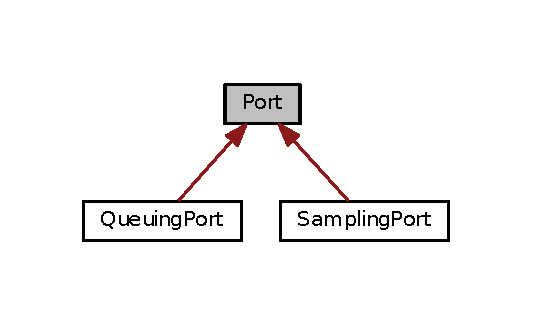
\includegraphics[width=256pt]{classPort__inherit__graph}
\end{center}
\end{figure}
\subsection*{Public Member Functions}
\begin{DoxyCompactItemize}
\item 
\hyperlink{classPort_a2cfb70a4b6d730e715042d646ec1d960}{Port} ()
\item 
\hyperlink{classPort_aecec2ad240af2b676c5e893ab04dddb0}{Port} (\hyperlink{structname__t}{name\+\_\+t} name, \hyperlink{apex__types_8h_a4e13487a80a5740717e19f7f693e06c3}{A\+P\+E\+X\+\_\+\+I\+N\+T\+E\+G\+ER} msg\+Size, \hyperlink{apex__types_8h_ae82fcf2f7f6f7966d59d9569049531a4}{P\+O\+R\+T\+\_\+\+D\+I\+R\+E\+C\+T\+I\+O\+N\+\_\+\+T\+Y\+PE} dir)
\item 
const \hyperlink{structname__t}{name\+\_\+t} \& \hyperlink{classPort_adab23e55c4a76ef09ae5a1b852989f29}{get\+Port\+Name} () const 
\item 
const \hyperlink{apex__types_8h_a4e13487a80a5740717e19f7f693e06c3}{A\+P\+E\+X\+\_\+\+I\+N\+T\+E\+G\+ER} \& \hyperlink{classPort_acbd4a7ffe1e9de9cbf4253ee9a149432}{get\+Max\+Message\+Size} () const 
\item 
const \hyperlink{apex__types_8h_ae82fcf2f7f6f7966d59d9569049531a4}{P\+O\+R\+T\+\_\+\+D\+I\+R\+E\+C\+T\+I\+O\+N\+\_\+\+T\+Y\+PE} \& \hyperlink{classPort_a722b6126b49af1c531caf7e0870bbe78}{get\+Direction} () const 
\end{DoxyCompactItemize}


\subsection{Constructor \& Destructor Documentation}
\index{Port@{Port}!Port@{Port}}
\index{Port@{Port}!Port@{Port}}
\subsubsection[{\texorpdfstring{Port()}{Port()}}]{\setlength{\rightskip}{0pt plus 5cm}Port\+::\+Port (
\begin{DoxyParamCaption}
{}
\end{DoxyParamCaption}
)\hspace{0.3cm}{\ttfamily [inline]}}\hypertarget{classPort_a2cfb70a4b6d730e715042d646ec1d960}{}\label{classPort_a2cfb70a4b6d730e715042d646ec1d960}
\index{Port@{Port}!Port@{Port}}
\index{Port@{Port}!Port@{Port}}
\subsubsection[{\texorpdfstring{Port(name\+\_\+t name, A\+P\+E\+X\+\_\+\+I\+N\+T\+E\+G\+E\+R msg\+Size, P\+O\+R\+T\+\_\+\+D\+I\+R\+E\+C\+T\+I\+O\+N\+\_\+\+T\+Y\+P\+E dir)}{Port(name_t name, APEX_INTEGER msgSize, PORT_DIRECTION_TYPE dir)}}]{\setlength{\rightskip}{0pt plus 5cm}Port\+::\+Port (
\begin{DoxyParamCaption}
\item[{{\bf name\+\_\+t}}]{name, }
\item[{{\bf A\+P\+E\+X\+\_\+\+I\+N\+T\+E\+G\+ER}}]{msg\+Size, }
\item[{{\bf P\+O\+R\+T\+\_\+\+D\+I\+R\+E\+C\+T\+I\+O\+N\+\_\+\+T\+Y\+PE}}]{dir}
\end{DoxyParamCaption}
)\hspace{0.3cm}{\ttfamily [inline]}}\hypertarget{classPort_aecec2ad240af2b676c5e893ab04dddb0}{}\label{classPort_aecec2ad240af2b676c5e893ab04dddb0}


\subsection{Member Function Documentation}
\index{Port@{Port}!get\+Direction@{get\+Direction}}
\index{get\+Direction@{get\+Direction}!Port@{Port}}
\subsubsection[{\texorpdfstring{get\+Direction() const }{getDirection() const }}]{\setlength{\rightskip}{0pt plus 5cm}const {\bf P\+O\+R\+T\+\_\+\+D\+I\+R\+E\+C\+T\+I\+O\+N\+\_\+\+T\+Y\+PE} \& Port\+::get\+Direction (
\begin{DoxyParamCaption}
{}
\end{DoxyParamCaption}
) const}\hypertarget{classPort_a722b6126b49af1c531caf7e0870bbe78}{}\label{classPort_a722b6126b49af1c531caf7e0870bbe78}
\index{Port@{Port}!get\+Max\+Message\+Size@{get\+Max\+Message\+Size}}
\index{get\+Max\+Message\+Size@{get\+Max\+Message\+Size}!Port@{Port}}
\subsubsection[{\texorpdfstring{get\+Max\+Message\+Size() const }{getMaxMessageSize() const }}]{\setlength{\rightskip}{0pt plus 5cm}const {\bf A\+P\+E\+X\+\_\+\+I\+N\+T\+E\+G\+ER} \& Port\+::get\+Max\+Message\+Size (
\begin{DoxyParamCaption}
{}
\end{DoxyParamCaption}
) const}\hypertarget{classPort_acbd4a7ffe1e9de9cbf4253ee9a149432}{}\label{classPort_acbd4a7ffe1e9de9cbf4253ee9a149432}
\index{Port@{Port}!get\+Port\+Name@{get\+Port\+Name}}
\index{get\+Port\+Name@{get\+Port\+Name}!Port@{Port}}
\subsubsection[{\texorpdfstring{get\+Port\+Name() const }{getPortName() const }}]{\setlength{\rightskip}{0pt plus 5cm}const {\bf name\+\_\+t} \& Port\+::get\+Port\+Name (
\begin{DoxyParamCaption}
{}
\end{DoxyParamCaption}
) const}\hypertarget{classPort_adab23e55c4a76ef09ae5a1b852989f29}{}\label{classPort_adab23e55c4a76ef09ae5a1b852989f29}


The documentation for this class was generated from the following files\+:\begin{DoxyCompactItemize}
\item 
src/types/include/\hyperlink{port_8hpp}{port.\+hpp}\item 
src/types/src/\hyperlink{port_8cpp}{port.\+cpp}\end{DoxyCompactItemize}

\hypertarget{classPortMapping}{}\section{Port\+Mapping Class Reference}
\label{classPortMapping}\index{Port\+Mapping@{Port\+Mapping}}


{\ttfamily \#include $<$port\+\_\+mapping.\+hpp$>$}

\subsection*{Public Member Functions}
\begin{DoxyCompactItemize}
\item 
\hyperlink{classPortMapping_a9de8f9098ed3dee87598dda1c91ec013}{Port\+Mapping} ()
\item 
\hyperlink{classPortMapping_a212cca06c51a90d31cf64f041c70154c}{Port\+Mapping} (\hyperlink{classPseudoPartition}{Pseudo\+Partition} pseudo\+Part)
\item 
\hyperlink{classPortMapping_a1c83b6b8fbf019986d410b65d259cb8f}{Port\+Mapping} (\hyperlink{classStandardPartition}{Standard\+Partition} standard\+Part)
\item 
const std\+::optional$<$ \hyperlink{classPseudoPartition}{Pseudo\+Partition} $>$ \& \hyperlink{classPortMapping_ad851407f0c7f287d85bec3f8e6b173ac}{get\+Pseudo\+Partition} () const 
\item 
const std\+::optional$<$ \hyperlink{classStandardPartition}{Standard\+Partition} $>$ \& \hyperlink{classPortMapping_af0f4571cf04a813df1589049485fd478}{get\+Standard\+Partition} () const 
\end{DoxyCompactItemize}


\subsection{Constructor \& Destructor Documentation}
\index{Port\+Mapping@{Port\+Mapping}!Port\+Mapping@{Port\+Mapping}}
\index{Port\+Mapping@{Port\+Mapping}!Port\+Mapping@{Port\+Mapping}}
\subsubsection[{\texorpdfstring{Port\+Mapping()}{PortMapping()}}]{\setlength{\rightskip}{0pt plus 5cm}Port\+Mapping\+::\+Port\+Mapping (
\begin{DoxyParamCaption}
{}
\end{DoxyParamCaption}
)\hspace{0.3cm}{\ttfamily [inline]}}\hypertarget{classPortMapping_a9de8f9098ed3dee87598dda1c91ec013}{}\label{classPortMapping_a9de8f9098ed3dee87598dda1c91ec013}
\index{Port\+Mapping@{Port\+Mapping}!Port\+Mapping@{Port\+Mapping}}
\index{Port\+Mapping@{Port\+Mapping}!Port\+Mapping@{Port\+Mapping}}
\subsubsection[{\texorpdfstring{Port\+Mapping(\+Pseudo\+Partition pseudo\+Part)}{PortMapping(PseudoPartition pseudoPart)}}]{\setlength{\rightskip}{0pt plus 5cm}Port\+Mapping\+::\+Port\+Mapping (
\begin{DoxyParamCaption}
\item[{{\bf Pseudo\+Partition}}]{pseudo\+Part}
\end{DoxyParamCaption}
)\hspace{0.3cm}{\ttfamily [inline]}}\hypertarget{classPortMapping_a212cca06c51a90d31cf64f041c70154c}{}\label{classPortMapping_a212cca06c51a90d31cf64f041c70154c}
\index{Port\+Mapping@{Port\+Mapping}!Port\+Mapping@{Port\+Mapping}}
\index{Port\+Mapping@{Port\+Mapping}!Port\+Mapping@{Port\+Mapping}}
\subsubsection[{\texorpdfstring{Port\+Mapping(\+Standard\+Partition standard\+Part)}{PortMapping(StandardPartition standardPart)}}]{\setlength{\rightskip}{0pt plus 5cm}Port\+Mapping\+::\+Port\+Mapping (
\begin{DoxyParamCaption}
\item[{{\bf Standard\+Partition}}]{standard\+Part}
\end{DoxyParamCaption}
)\hspace{0.3cm}{\ttfamily [inline]}}\hypertarget{classPortMapping_a1c83b6b8fbf019986d410b65d259cb8f}{}\label{classPortMapping_a1c83b6b8fbf019986d410b65d259cb8f}


\subsection{Member Function Documentation}
\index{Port\+Mapping@{Port\+Mapping}!get\+Pseudo\+Partition@{get\+Pseudo\+Partition}}
\index{get\+Pseudo\+Partition@{get\+Pseudo\+Partition}!Port\+Mapping@{Port\+Mapping}}
\subsubsection[{\texorpdfstring{get\+Pseudo\+Partition() const }{getPseudoPartition() const }}]{\setlength{\rightskip}{0pt plus 5cm}const std\+::optional$<$ {\bf Pseudo\+Partition} $>$ \& Port\+Mapping\+::get\+Pseudo\+Partition (
\begin{DoxyParamCaption}
{}
\end{DoxyParamCaption}
) const}\hypertarget{classPortMapping_ad851407f0c7f287d85bec3f8e6b173ac}{}\label{classPortMapping_ad851407f0c7f287d85bec3f8e6b173ac}
\index{Port\+Mapping@{Port\+Mapping}!get\+Standard\+Partition@{get\+Standard\+Partition}}
\index{get\+Standard\+Partition@{get\+Standard\+Partition}!Port\+Mapping@{Port\+Mapping}}
\subsubsection[{\texorpdfstring{get\+Standard\+Partition() const }{getStandardPartition() const }}]{\setlength{\rightskip}{0pt plus 5cm}const std\+::optional$<$ {\bf Standard\+Partition} $>$ \& Port\+Mapping\+::get\+Standard\+Partition (
\begin{DoxyParamCaption}
{}
\end{DoxyParamCaption}
) const}\hypertarget{classPortMapping_af0f4571cf04a813df1589049485fd478}{}\label{classPortMapping_af0f4571cf04a813df1589049485fd478}


The documentation for this class was generated from the following files\+:\begin{DoxyCompactItemize}
\item 
src/types/include/\hyperlink{port__mapping_8hpp}{port\+\_\+mapping.\+hpp}\item 
src/types/src/\hyperlink{port__mapping_8cpp}{port\+\_\+mapping.\+cpp}\end{DoxyCompactItemize}

\hypertarget{classPrimeProc}{}\section{Prime\+Proc Class Reference}
\label{classPrimeProc}\index{Prime\+Proc@{Prime\+Proc}}


{\ttfamily \#include $<$primeproc.\+h$>$}



Inheritance diagram for Prime\+Proc\+:
\nopagebreak
\begin{figure}[H]
\begin{center}
\leavevmode
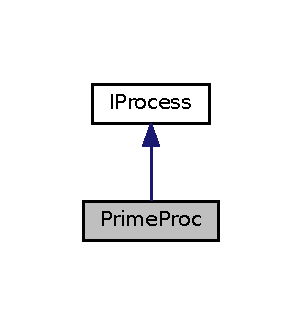
\includegraphics[width=145pt]{classPrimeProc__inherit__graph}
\end{center}
\end{figure}


Collaboration diagram for Prime\+Proc\+:
\nopagebreak
\begin{figure}[H]
\begin{center}
\leavevmode
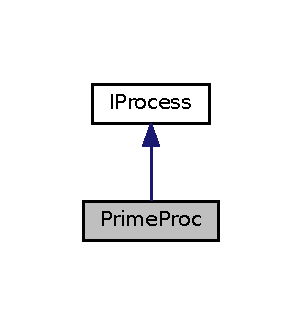
\includegraphics[width=145pt]{classPrimeProc__coll__graph}
\end{center}
\end{figure}
\subsection*{Public Member Functions}
\begin{DoxyCompactItemize}
\item 
\hyperlink{classPrimeProc_a77faab1b7b50b09b6a1dac931183acd6}{Prime\+Proc} (const char $\ast$\hyperlink{classIProcess_ad8e9a2d6537a7671236456af14b3a5b7}{name\+Ref}, C\+Logger \&logger)
\item 
\hyperlink{classPrimeProc_a5765b088769c328c7e1fbbf4af5b0395}{$\sim$\+Prime\+Proc} ()
\item 
void \hyperlink{classPrimeProc_a650b1ea0ed282f5137b594a8f916990a}{run} ()
\item 
bool \hyperlink{classPrimeProc_ac8b98010d54586414e26f84aec7c9067}{initialise} ()
\item 
int \hyperlink{classPrimeProc_ad24fb156156bb16d6018c549c2474dfc}{fib} (int n)
\end{DoxyCompactItemize}
\subsection*{Protected Attributes}
\begin{DoxyCompactItemize}
\item 
C\+Logger \& \hyperlink{classPrimeProc_ae88d8aee3d4b7dedd75888b83b3345de}{m\+Logger}
\end{DoxyCompactItemize}


\subsection{Constructor \& Destructor Documentation}
\index{Prime\+Proc@{Prime\+Proc}!Prime\+Proc@{Prime\+Proc}}
\index{Prime\+Proc@{Prime\+Proc}!Prime\+Proc@{Prime\+Proc}}
\subsubsection[{\texorpdfstring{Prime\+Proc(const char $\ast$name\+Ref, C\+Logger \&logger)}{PrimeProc(const char *nameRef, CLogger &logger)}}]{\setlength{\rightskip}{0pt plus 5cm}Prime\+Proc\+::\+Prime\+Proc (
\begin{DoxyParamCaption}
\item[{const char $\ast$}]{name\+Ref, }
\item[{C\+Logger \&}]{logger}
\end{DoxyParamCaption}
)}\hypertarget{classPrimeProc_a77faab1b7b50b09b6a1dac931183acd6}{}\label{classPrimeProc_a77faab1b7b50b09b6a1dac931183acd6}
\index{Prime\+Proc@{Prime\+Proc}!````~Prime\+Proc@{$\sim$\+Prime\+Proc}}
\index{````~Prime\+Proc@{$\sim$\+Prime\+Proc}!Prime\+Proc@{Prime\+Proc}}
\subsubsection[{\texorpdfstring{$\sim$\+Prime\+Proc()}{~PrimeProc()}}]{\setlength{\rightskip}{0pt plus 5cm}Prime\+Proc\+::$\sim$\+Prime\+Proc (
\begin{DoxyParamCaption}
{}
\end{DoxyParamCaption}
)\hspace{0.3cm}{\ttfamily [inline]}}\hypertarget{classPrimeProc_a5765b088769c328c7e1fbbf4af5b0395}{}\label{classPrimeProc_a5765b088769c328c7e1fbbf4af5b0395}


\subsection{Member Function Documentation}
\index{Prime\+Proc@{Prime\+Proc}!fib@{fib}}
\index{fib@{fib}!Prime\+Proc@{Prime\+Proc}}
\subsubsection[{\texorpdfstring{fib(int n)}{fib(int n)}}]{\setlength{\rightskip}{0pt plus 5cm}int Prime\+Proc\+::fib (
\begin{DoxyParamCaption}
\item[{int}]{n}
\end{DoxyParamCaption}
)}\hypertarget{classPrimeProc_ad24fb156156bb16d6018c549c2474dfc}{}\label{classPrimeProc_ad24fb156156bb16d6018c549c2474dfc}
\index{Prime\+Proc@{Prime\+Proc}!initialise@{initialise}}
\index{initialise@{initialise}!Prime\+Proc@{Prime\+Proc}}
\subsubsection[{\texorpdfstring{initialise()}{initialise()}}]{\setlength{\rightskip}{0pt plus 5cm}bool Prime\+Proc\+::initialise (
\begin{DoxyParamCaption}
{}
\end{DoxyParamCaption}
)\hspace{0.3cm}{\ttfamily [virtual]}}\hypertarget{classPrimeProc_ac8b98010d54586414e26f84aec7c9067}{}\label{classPrimeProc_ac8b98010d54586414e26f84aec7c9067}


Implements \hyperlink{classIProcess_a238bce621ce9e6cf7c9dc4201bdfb8b2}{I\+Process}.

\index{Prime\+Proc@{Prime\+Proc}!run@{run}}
\index{run@{run}!Prime\+Proc@{Prime\+Proc}}
\subsubsection[{\texorpdfstring{run()}{run()}}]{\setlength{\rightskip}{0pt plus 5cm}void Prime\+Proc\+::run (
\begin{DoxyParamCaption}
{}
\end{DoxyParamCaption}
)\hspace{0.3cm}{\ttfamily [virtual]}}\hypertarget{classPrimeProc_a650b1ea0ed282f5137b594a8f916990a}{}\label{classPrimeProc_a650b1ea0ed282f5137b594a8f916990a}


Implements \hyperlink{classIProcess_ae2a840bd8730af48b04254387ba3f9e3}{I\+Process}.



\subsection{Member Data Documentation}
\index{Prime\+Proc@{Prime\+Proc}!m\+Logger@{m\+Logger}}
\index{m\+Logger@{m\+Logger}!Prime\+Proc@{Prime\+Proc}}
\subsubsection[{\texorpdfstring{m\+Logger}{mLogger}}]{\setlength{\rightskip}{0pt plus 5cm}C\+Logger\& Prime\+Proc\+::m\+Logger\hspace{0.3cm}{\ttfamily [protected]}}\hypertarget{classPrimeProc_ae88d8aee3d4b7dedd75888b83b3345de}{}\label{classPrimeProc_ae88d8aee3d4b7dedd75888b83b3345de}


The documentation for this class was generated from the following files\+:\begin{DoxyCompactItemize}
\item 
src/apps/\hyperlink{primeproc_8h}{primeproc.\+h}\item 
src/apps/\hyperlink{primeproc_8cpp}{primeproc.\+cpp}\end{DoxyCompactItemize}

\hypertarget{classProcess}{}\section{Process Class Reference}
\label{classProcess}\index{Process@{Process}}


{\ttfamily \#include $<$process.\+hpp$>$}

\subsection*{Public Member Functions}
\begin{DoxyCompactItemize}
\item 
\hyperlink{classProcess_a60dea03f63b524f3d5ffeffab78d2d86}{Process} (\hyperlink{structname__t}{name\+\_\+t} name, \hyperlink{general__types_8hpp_a0edc3a86ddf4aa205c6882b61cd7b4e9}{dec\+Or\+Hex\+\_\+t} identifier, \hyperlink{general__types_8hpp_a0edc3a86ddf4aa205c6882b61cd7b4e9}{dec\+Or\+Hex\+\_\+t} priority, \hyperlink{general__types_8hpp_a0edc3a86ddf4aa205c6882b61cd7b4e9}{dec\+Or\+Hex\+\_\+t} period)
\item 
\hyperlink{classProcess_a9f4553eac74c657bb451f390c17d6bea}{Process} ()
\item 
\hyperlink{classProcess_a9033f4b620c1fc8521fb2e51353f8269}{Process} (\hyperlink{structPROCESS__ATTRIBUTE__TYPE}{P\+R\+O\+C\+E\+S\+S\+\_\+\+A\+T\+T\+R\+I\+B\+U\+T\+E\+\_\+\+T\+Y\+PE} attr, \hyperlink{structPROCESS__STATUS__TYPE}{P\+R\+O\+C\+E\+S\+S\+\_\+\+S\+T\+A\+T\+U\+S\+\_\+\+T\+Y\+PE} status)
\item 
const \hyperlink{structPROCESS__STATUS__TYPE}{P\+R\+O\+C\+E\+S\+S\+\_\+\+S\+T\+A\+T\+U\+S\+\_\+\+T\+Y\+PE} \& \hyperlink{classProcess_a70d2f9855b4fd3eae3288e18e376e747}{get\+Status} () const 
\item 
const \hyperlink{structPROCESS__ATTRIBUTE__TYPE}{P\+R\+O\+C\+E\+S\+S\+\_\+\+A\+T\+T\+R\+I\+B\+U\+T\+E\+\_\+\+T\+Y\+PE} \& \hyperlink{classProcess_a1a990dca63444f3e642ca6522ec35440}{get\+Attributes} () const 
\end{DoxyCompactItemize}


\subsection{Constructor \& Destructor Documentation}
\index{Process@{Process}!Process@{Process}}
\index{Process@{Process}!Process@{Process}}
\subsubsection[{\texorpdfstring{Process(name\+\_\+t name, dec\+Or\+Hex\+\_\+t identifier, dec\+Or\+Hex\+\_\+t priority, dec\+Or\+Hex\+\_\+t period)}{Process(name_t name, decOrHex_t identifier, decOrHex_t priority, decOrHex_t period)}}]{\setlength{\rightskip}{0pt plus 5cm}Process\+::\+Process (
\begin{DoxyParamCaption}
\item[{{\bf name\+\_\+t}}]{name, }
\item[{{\bf dec\+Or\+Hex\+\_\+t}}]{identifier, }
\item[{{\bf dec\+Or\+Hex\+\_\+t}}]{priority, }
\item[{{\bf dec\+Or\+Hex\+\_\+t}}]{period}
\end{DoxyParamCaption}
)\hspace{0.3cm}{\ttfamily [inline]}}\hypertarget{classProcess_a60dea03f63b524f3d5ffeffab78d2d86}{}\label{classProcess_a60dea03f63b524f3d5ffeffab78d2d86}
\index{Process@{Process}!Process@{Process}}
\index{Process@{Process}!Process@{Process}}
\subsubsection[{\texorpdfstring{Process()}{Process()}}]{\setlength{\rightskip}{0pt plus 5cm}Process\+::\+Process (
\begin{DoxyParamCaption}
{}
\end{DoxyParamCaption}
)\hspace{0.3cm}{\ttfamily [inline]}}\hypertarget{classProcess_a9f4553eac74c657bb451f390c17d6bea}{}\label{classProcess_a9f4553eac74c657bb451f390c17d6bea}
\index{Process@{Process}!Process@{Process}}
\index{Process@{Process}!Process@{Process}}
\subsubsection[{\texorpdfstring{Process(\+P\+R\+O\+C\+E\+S\+S\+\_\+\+A\+T\+T\+R\+I\+B\+U\+T\+E\+\_\+\+T\+Y\+P\+E attr, P\+R\+O\+C\+E\+S\+S\+\_\+\+S\+T\+A\+T\+U\+S\+\_\+\+T\+Y\+P\+E status)}{Process(PROCESS_ATTRIBUTE_TYPE attr, PROCESS_STATUS_TYPE status)}}]{\setlength{\rightskip}{0pt plus 5cm}Process\+::\+Process (
\begin{DoxyParamCaption}
\item[{{\bf P\+R\+O\+C\+E\+S\+S\+\_\+\+A\+T\+T\+R\+I\+B\+U\+T\+E\+\_\+\+T\+Y\+PE}}]{attr, }
\item[{{\bf P\+R\+O\+C\+E\+S\+S\+\_\+\+S\+T\+A\+T\+U\+S\+\_\+\+T\+Y\+PE}}]{status}
\end{DoxyParamCaption}
)\hspace{0.3cm}{\ttfamily [inline]}}\hypertarget{classProcess_a9033f4b620c1fc8521fb2e51353f8269}{}\label{classProcess_a9033f4b620c1fc8521fb2e51353f8269}


\subsection{Member Function Documentation}
\index{Process@{Process}!get\+Attributes@{get\+Attributes}}
\index{get\+Attributes@{get\+Attributes}!Process@{Process}}
\subsubsection[{\texorpdfstring{get\+Attributes() const }{getAttributes() const }}]{\setlength{\rightskip}{0pt plus 5cm}const {\bf P\+R\+O\+C\+E\+S\+S\+\_\+\+A\+T\+T\+R\+I\+B\+U\+T\+E\+\_\+\+T\+Y\+PE} \& Process\+::get\+Attributes (
\begin{DoxyParamCaption}
{}
\end{DoxyParamCaption}
) const}\hypertarget{classProcess_a1a990dca63444f3e642ca6522ec35440}{}\label{classProcess_a1a990dca63444f3e642ca6522ec35440}
\index{Process@{Process}!get\+Status@{get\+Status}}
\index{get\+Status@{get\+Status}!Process@{Process}}
\subsubsection[{\texorpdfstring{get\+Status() const }{getStatus() const }}]{\setlength{\rightskip}{0pt plus 5cm}const {\bf P\+R\+O\+C\+E\+S\+S\+\_\+\+S\+T\+A\+T\+U\+S\+\_\+\+T\+Y\+PE} \& Process\+::get\+Status (
\begin{DoxyParamCaption}
{}
\end{DoxyParamCaption}
) const}\hypertarget{classProcess_a70d2f9855b4fd3eae3288e18e376e747}{}\label{classProcess_a70d2f9855b4fd3eae3288e18e376e747}


The documentation for this class was generated from the following files\+:\begin{DoxyCompactItemize}
\item 
src/types/include/\hyperlink{process_8hpp}{process.\+hpp}\item 
src/types/src/\hyperlink{process_8cpp}{process.\+cpp}\end{DoxyCompactItemize}

\hypertarget{structPROCESS__ATTRIBUTE__TYPE}{}\section{P\+R\+O\+C\+E\+S\+S\+\_\+\+A\+T\+T\+R\+I\+B\+U\+T\+E\+\_\+\+T\+Y\+PE Struct Reference}
\label{structPROCESS__ATTRIBUTE__TYPE}\index{P\+R\+O\+C\+E\+S\+S\+\_\+\+A\+T\+T\+R\+I\+B\+U\+T\+E\+\_\+\+T\+Y\+PE@{P\+R\+O\+C\+E\+S\+S\+\_\+\+A\+T\+T\+R\+I\+B\+U\+T\+E\+\_\+\+T\+Y\+PE}}


{\ttfamily \#include $<$apex\+\_\+process.\+h$>$}



Collaboration diagram for P\+R\+O\+C\+E\+S\+S\+\_\+\+A\+T\+T\+R\+I\+B\+U\+T\+E\+\_\+\+T\+Y\+PE\+:
\nopagebreak
\begin{figure}[H]
\begin{center}
\leavevmode
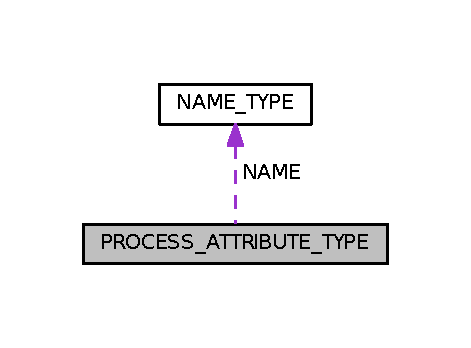
\includegraphics[width=226pt]{structPROCESS__ATTRIBUTE__TYPE__coll__graph}
\end{center}
\end{figure}
\subsection*{Public Attributes}
\begin{DoxyCompactItemize}
\item 
\hyperlink{apex__types_8h_a78cd52c2621ddf2eda68fcd4bedbc1a7}{S\+Y\+S\+T\+E\+M\+\_\+\+T\+I\+M\+E\+\_\+\+T\+Y\+PE} \hyperlink{structPROCESS__ATTRIBUTE__TYPE_af571eb32c097ecf8423b40e069200d0d}{P\+E\+R\+I\+OD}
\item 
\hyperlink{apex__types_8h_a78cd52c2621ddf2eda68fcd4bedbc1a7}{S\+Y\+S\+T\+E\+M\+\_\+\+T\+I\+M\+E\+\_\+\+T\+Y\+PE} \hyperlink{structPROCESS__ATTRIBUTE__TYPE_aa3a2776010bcd8a9c21ea08013db926e}{T\+I\+M\+E\+\_\+\+C\+A\+P\+A\+C\+I\+TY}
\item 
\hyperlink{apex__types_8h_afad87659fcb2bad73146a13b260290b9}{S\+Y\+S\+T\+E\+M\+\_\+\+A\+D\+D\+R\+E\+S\+S\+\_\+\+T\+Y\+PE} \hyperlink{structPROCESS__ATTRIBUTE__TYPE_a114dee662eb2d6aa73c01cba161ff9cf}{E\+N\+T\+R\+Y\+\_\+\+P\+O\+I\+NT}
\item 
\hyperlink{apex__process_8h_a88a1e60035e9edf9ff430765543659b2}{S\+T\+A\+C\+K\+\_\+\+S\+I\+Z\+E\+\_\+\+T\+Y\+PE} \hyperlink{structPROCESS__ATTRIBUTE__TYPE_a840fae988efaf861b2ca2ac27fbf1339}{S\+T\+A\+C\+K\+\_\+\+S\+I\+ZE}
\item 
\hyperlink{apex__process_8h_a2185443fe5bfda31ff9cce2071f1b18c}{P\+R\+I\+O\+R\+I\+T\+Y\+\_\+\+T\+Y\+PE} \hyperlink{structPROCESS__ATTRIBUTE__TYPE_ae964c35a6c5d325d3070ec54dc4c0cb0}{B\+A\+S\+E\+\_\+\+P\+R\+I\+O\+R\+I\+TY}
\item 
\hyperlink{apex__process_8h_a930759cec98a9372ee6b92c4c20223fe}{D\+E\+A\+D\+L\+I\+N\+E\+\_\+\+T\+Y\+PE} \hyperlink{structPROCESS__ATTRIBUTE__TYPE_afc0e1313a66a458071d58be90d818eae}{D\+E\+A\+D\+L\+I\+NE}
\item 
\hyperlink{apex__process_8h_a50887e4c49611fad19176906f38db47c}{P\+R\+O\+C\+E\+S\+S\+\_\+\+N\+A\+M\+E\+\_\+\+T\+Y\+PE} \hyperlink{structPROCESS__ATTRIBUTE__TYPE_afe04bf9682eabb1bcca2a2059ce97cee}{N\+A\+ME}
\end{DoxyCompactItemize}


\subsection{Member Data Documentation}
\index{P\+R\+O\+C\+E\+S\+S\+\_\+\+A\+T\+T\+R\+I\+B\+U\+T\+E\+\_\+\+T\+Y\+PE@{P\+R\+O\+C\+E\+S\+S\+\_\+\+A\+T\+T\+R\+I\+B\+U\+T\+E\+\_\+\+T\+Y\+PE}!B\+A\+S\+E\+\_\+\+P\+R\+I\+O\+R\+I\+TY@{B\+A\+S\+E\+\_\+\+P\+R\+I\+O\+R\+I\+TY}}
\index{B\+A\+S\+E\+\_\+\+P\+R\+I\+O\+R\+I\+TY@{B\+A\+S\+E\+\_\+\+P\+R\+I\+O\+R\+I\+TY}!P\+R\+O\+C\+E\+S\+S\+\_\+\+A\+T\+T\+R\+I\+B\+U\+T\+E\+\_\+\+T\+Y\+PE@{P\+R\+O\+C\+E\+S\+S\+\_\+\+A\+T\+T\+R\+I\+B\+U\+T\+E\+\_\+\+T\+Y\+PE}}
\subsubsection[{\texorpdfstring{B\+A\+S\+E\+\_\+\+P\+R\+I\+O\+R\+I\+TY}{BASE_PRIORITY}}]{\setlength{\rightskip}{0pt plus 5cm}{\bf P\+R\+I\+O\+R\+I\+T\+Y\+\_\+\+T\+Y\+PE} P\+R\+O\+C\+E\+S\+S\+\_\+\+A\+T\+T\+R\+I\+B\+U\+T\+E\+\_\+\+T\+Y\+P\+E\+::\+B\+A\+S\+E\+\_\+\+P\+R\+I\+O\+R\+I\+TY}\hypertarget{structPROCESS__ATTRIBUTE__TYPE_ae964c35a6c5d325d3070ec54dc4c0cb0}{}\label{structPROCESS__ATTRIBUTE__TYPE_ae964c35a6c5d325d3070ec54dc4c0cb0}
\index{P\+R\+O\+C\+E\+S\+S\+\_\+\+A\+T\+T\+R\+I\+B\+U\+T\+E\+\_\+\+T\+Y\+PE@{P\+R\+O\+C\+E\+S\+S\+\_\+\+A\+T\+T\+R\+I\+B\+U\+T\+E\+\_\+\+T\+Y\+PE}!D\+E\+A\+D\+L\+I\+NE@{D\+E\+A\+D\+L\+I\+NE}}
\index{D\+E\+A\+D\+L\+I\+NE@{D\+E\+A\+D\+L\+I\+NE}!P\+R\+O\+C\+E\+S\+S\+\_\+\+A\+T\+T\+R\+I\+B\+U\+T\+E\+\_\+\+T\+Y\+PE@{P\+R\+O\+C\+E\+S\+S\+\_\+\+A\+T\+T\+R\+I\+B\+U\+T\+E\+\_\+\+T\+Y\+PE}}
\subsubsection[{\texorpdfstring{D\+E\+A\+D\+L\+I\+NE}{DEADLINE}}]{\setlength{\rightskip}{0pt plus 5cm}{\bf D\+E\+A\+D\+L\+I\+N\+E\+\_\+\+T\+Y\+PE} P\+R\+O\+C\+E\+S\+S\+\_\+\+A\+T\+T\+R\+I\+B\+U\+T\+E\+\_\+\+T\+Y\+P\+E\+::\+D\+E\+A\+D\+L\+I\+NE}\hypertarget{structPROCESS__ATTRIBUTE__TYPE_afc0e1313a66a458071d58be90d818eae}{}\label{structPROCESS__ATTRIBUTE__TYPE_afc0e1313a66a458071d58be90d818eae}
\index{P\+R\+O\+C\+E\+S\+S\+\_\+\+A\+T\+T\+R\+I\+B\+U\+T\+E\+\_\+\+T\+Y\+PE@{P\+R\+O\+C\+E\+S\+S\+\_\+\+A\+T\+T\+R\+I\+B\+U\+T\+E\+\_\+\+T\+Y\+PE}!E\+N\+T\+R\+Y\+\_\+\+P\+O\+I\+NT@{E\+N\+T\+R\+Y\+\_\+\+P\+O\+I\+NT}}
\index{E\+N\+T\+R\+Y\+\_\+\+P\+O\+I\+NT@{E\+N\+T\+R\+Y\+\_\+\+P\+O\+I\+NT}!P\+R\+O\+C\+E\+S\+S\+\_\+\+A\+T\+T\+R\+I\+B\+U\+T\+E\+\_\+\+T\+Y\+PE@{P\+R\+O\+C\+E\+S\+S\+\_\+\+A\+T\+T\+R\+I\+B\+U\+T\+E\+\_\+\+T\+Y\+PE}}
\subsubsection[{\texorpdfstring{E\+N\+T\+R\+Y\+\_\+\+P\+O\+I\+NT}{ENTRY_POINT}}]{\setlength{\rightskip}{0pt plus 5cm}{\bf S\+Y\+S\+T\+E\+M\+\_\+\+A\+D\+D\+R\+E\+S\+S\+\_\+\+T\+Y\+PE} P\+R\+O\+C\+E\+S\+S\+\_\+\+A\+T\+T\+R\+I\+B\+U\+T\+E\+\_\+\+T\+Y\+P\+E\+::\+E\+N\+T\+R\+Y\+\_\+\+P\+O\+I\+NT}\hypertarget{structPROCESS__ATTRIBUTE__TYPE_a114dee662eb2d6aa73c01cba161ff9cf}{}\label{structPROCESS__ATTRIBUTE__TYPE_a114dee662eb2d6aa73c01cba161ff9cf}
\index{P\+R\+O\+C\+E\+S\+S\+\_\+\+A\+T\+T\+R\+I\+B\+U\+T\+E\+\_\+\+T\+Y\+PE@{P\+R\+O\+C\+E\+S\+S\+\_\+\+A\+T\+T\+R\+I\+B\+U\+T\+E\+\_\+\+T\+Y\+PE}!N\+A\+ME@{N\+A\+ME}}
\index{N\+A\+ME@{N\+A\+ME}!P\+R\+O\+C\+E\+S\+S\+\_\+\+A\+T\+T\+R\+I\+B\+U\+T\+E\+\_\+\+T\+Y\+PE@{P\+R\+O\+C\+E\+S\+S\+\_\+\+A\+T\+T\+R\+I\+B\+U\+T\+E\+\_\+\+T\+Y\+PE}}
\subsubsection[{\texorpdfstring{N\+A\+ME}{NAME}}]{\setlength{\rightskip}{0pt plus 5cm}{\bf P\+R\+O\+C\+E\+S\+S\+\_\+\+N\+A\+M\+E\+\_\+\+T\+Y\+PE} P\+R\+O\+C\+E\+S\+S\+\_\+\+A\+T\+T\+R\+I\+B\+U\+T\+E\+\_\+\+T\+Y\+P\+E\+::\+N\+A\+ME}\hypertarget{structPROCESS__ATTRIBUTE__TYPE_afe04bf9682eabb1bcca2a2059ce97cee}{}\label{structPROCESS__ATTRIBUTE__TYPE_afe04bf9682eabb1bcca2a2059ce97cee}
\index{P\+R\+O\+C\+E\+S\+S\+\_\+\+A\+T\+T\+R\+I\+B\+U\+T\+E\+\_\+\+T\+Y\+PE@{P\+R\+O\+C\+E\+S\+S\+\_\+\+A\+T\+T\+R\+I\+B\+U\+T\+E\+\_\+\+T\+Y\+PE}!P\+E\+R\+I\+OD@{P\+E\+R\+I\+OD}}
\index{P\+E\+R\+I\+OD@{P\+E\+R\+I\+OD}!P\+R\+O\+C\+E\+S\+S\+\_\+\+A\+T\+T\+R\+I\+B\+U\+T\+E\+\_\+\+T\+Y\+PE@{P\+R\+O\+C\+E\+S\+S\+\_\+\+A\+T\+T\+R\+I\+B\+U\+T\+E\+\_\+\+T\+Y\+PE}}
\subsubsection[{\texorpdfstring{P\+E\+R\+I\+OD}{PERIOD}}]{\setlength{\rightskip}{0pt plus 5cm}{\bf S\+Y\+S\+T\+E\+M\+\_\+\+T\+I\+M\+E\+\_\+\+T\+Y\+PE} P\+R\+O\+C\+E\+S\+S\+\_\+\+A\+T\+T\+R\+I\+B\+U\+T\+E\+\_\+\+T\+Y\+P\+E\+::\+P\+E\+R\+I\+OD}\hypertarget{structPROCESS__ATTRIBUTE__TYPE_af571eb32c097ecf8423b40e069200d0d}{}\label{structPROCESS__ATTRIBUTE__TYPE_af571eb32c097ecf8423b40e069200d0d}
\index{P\+R\+O\+C\+E\+S\+S\+\_\+\+A\+T\+T\+R\+I\+B\+U\+T\+E\+\_\+\+T\+Y\+PE@{P\+R\+O\+C\+E\+S\+S\+\_\+\+A\+T\+T\+R\+I\+B\+U\+T\+E\+\_\+\+T\+Y\+PE}!S\+T\+A\+C\+K\+\_\+\+S\+I\+ZE@{S\+T\+A\+C\+K\+\_\+\+S\+I\+ZE}}
\index{S\+T\+A\+C\+K\+\_\+\+S\+I\+ZE@{S\+T\+A\+C\+K\+\_\+\+S\+I\+ZE}!P\+R\+O\+C\+E\+S\+S\+\_\+\+A\+T\+T\+R\+I\+B\+U\+T\+E\+\_\+\+T\+Y\+PE@{P\+R\+O\+C\+E\+S\+S\+\_\+\+A\+T\+T\+R\+I\+B\+U\+T\+E\+\_\+\+T\+Y\+PE}}
\subsubsection[{\texorpdfstring{S\+T\+A\+C\+K\+\_\+\+S\+I\+ZE}{STACK_SIZE}}]{\setlength{\rightskip}{0pt plus 5cm}{\bf S\+T\+A\+C\+K\+\_\+\+S\+I\+Z\+E\+\_\+\+T\+Y\+PE} P\+R\+O\+C\+E\+S\+S\+\_\+\+A\+T\+T\+R\+I\+B\+U\+T\+E\+\_\+\+T\+Y\+P\+E\+::\+S\+T\+A\+C\+K\+\_\+\+S\+I\+ZE}\hypertarget{structPROCESS__ATTRIBUTE__TYPE_a840fae988efaf861b2ca2ac27fbf1339}{}\label{structPROCESS__ATTRIBUTE__TYPE_a840fae988efaf861b2ca2ac27fbf1339}
\index{P\+R\+O\+C\+E\+S\+S\+\_\+\+A\+T\+T\+R\+I\+B\+U\+T\+E\+\_\+\+T\+Y\+PE@{P\+R\+O\+C\+E\+S\+S\+\_\+\+A\+T\+T\+R\+I\+B\+U\+T\+E\+\_\+\+T\+Y\+PE}!T\+I\+M\+E\+\_\+\+C\+A\+P\+A\+C\+I\+TY@{T\+I\+M\+E\+\_\+\+C\+A\+P\+A\+C\+I\+TY}}
\index{T\+I\+M\+E\+\_\+\+C\+A\+P\+A\+C\+I\+TY@{T\+I\+M\+E\+\_\+\+C\+A\+P\+A\+C\+I\+TY}!P\+R\+O\+C\+E\+S\+S\+\_\+\+A\+T\+T\+R\+I\+B\+U\+T\+E\+\_\+\+T\+Y\+PE@{P\+R\+O\+C\+E\+S\+S\+\_\+\+A\+T\+T\+R\+I\+B\+U\+T\+E\+\_\+\+T\+Y\+PE}}
\subsubsection[{\texorpdfstring{T\+I\+M\+E\+\_\+\+C\+A\+P\+A\+C\+I\+TY}{TIME_CAPACITY}}]{\setlength{\rightskip}{0pt plus 5cm}{\bf S\+Y\+S\+T\+E\+M\+\_\+\+T\+I\+M\+E\+\_\+\+T\+Y\+PE} P\+R\+O\+C\+E\+S\+S\+\_\+\+A\+T\+T\+R\+I\+B\+U\+T\+E\+\_\+\+T\+Y\+P\+E\+::\+T\+I\+M\+E\+\_\+\+C\+A\+P\+A\+C\+I\+TY}\hypertarget{structPROCESS__ATTRIBUTE__TYPE_aa3a2776010bcd8a9c21ea08013db926e}{}\label{structPROCESS__ATTRIBUTE__TYPE_aa3a2776010bcd8a9c21ea08013db926e}


The documentation for this struct was generated from the following file\+:\begin{DoxyCompactItemize}
\item 
src/libuser/apex/\hyperlink{apex__process_8h}{apex\+\_\+process.\+h}\end{DoxyCompactItemize}

\hypertarget{structPROCESS__STATUS__TYPE}{}\section{P\+R\+O\+C\+E\+S\+S\+\_\+\+S\+T\+A\+T\+U\+S\+\_\+\+T\+Y\+PE Struct Reference}
\label{structPROCESS__STATUS__TYPE}\index{P\+R\+O\+C\+E\+S\+S\+\_\+\+S\+T\+A\+T\+U\+S\+\_\+\+T\+Y\+PE@{P\+R\+O\+C\+E\+S\+S\+\_\+\+S\+T\+A\+T\+U\+S\+\_\+\+T\+Y\+PE}}


{\ttfamily \#include $<$apex\+\_\+process.\+h$>$}



Collaboration diagram for P\+R\+O\+C\+E\+S\+S\+\_\+\+S\+T\+A\+T\+U\+S\+\_\+\+T\+Y\+PE\+:
\nopagebreak
\begin{figure}[H]
\begin{center}
\leavevmode
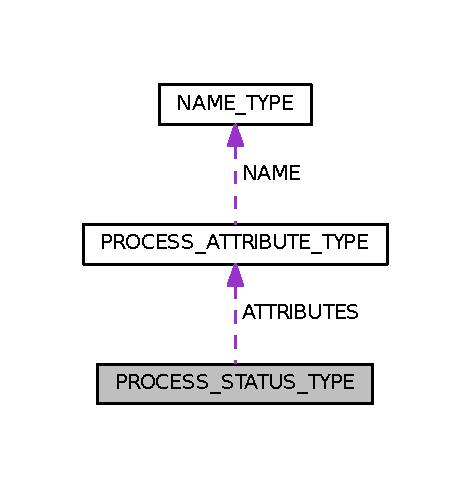
\includegraphics[width=226pt]{structPROCESS__STATUS__TYPE__coll__graph}
\end{center}
\end{figure}
\subsection*{Public Attributes}
\begin{DoxyCompactItemize}
\item 
\hyperlink{apex__types_8h_a78cd52c2621ddf2eda68fcd4bedbc1a7}{S\+Y\+S\+T\+E\+M\+\_\+\+T\+I\+M\+E\+\_\+\+T\+Y\+PE} \hyperlink{structPROCESS__STATUS__TYPE_a6d80b5fda37441bd85be66724c8e39ea}{D\+E\+A\+D\+L\+I\+N\+E\+\_\+\+T\+I\+ME}
\item 
\hyperlink{apex__process_8h_a2185443fe5bfda31ff9cce2071f1b18c}{P\+R\+I\+O\+R\+I\+T\+Y\+\_\+\+T\+Y\+PE} \hyperlink{structPROCESS__STATUS__TYPE_a09a4859e0a86c5d194725cffa73e3580}{C\+U\+R\+R\+E\+N\+T\+\_\+\+P\+R\+I\+O\+R\+I\+TY}
\item 
\hyperlink{apex__process_8h_a79733d58c516410711ac89880fa90aa7}{P\+R\+O\+C\+E\+S\+S\+\_\+\+S\+T\+A\+T\+E\+\_\+\+T\+Y\+PE} \hyperlink{structPROCESS__STATUS__TYPE_a31a78e79d64f384b6f628c5441e6df90}{P\+R\+O\+C\+E\+S\+S\+\_\+\+S\+T\+A\+TE}
\item 
\hyperlink{structPROCESS__ATTRIBUTE__TYPE}{P\+R\+O\+C\+E\+S\+S\+\_\+\+A\+T\+T\+R\+I\+B\+U\+T\+E\+\_\+\+T\+Y\+PE} \hyperlink{structPROCESS__STATUS__TYPE_a54f0a046bf957db798482952628b4364}{A\+T\+T\+R\+I\+B\+U\+T\+ES}
\end{DoxyCompactItemize}


\subsection{Member Data Documentation}
\index{P\+R\+O\+C\+E\+S\+S\+\_\+\+S\+T\+A\+T\+U\+S\+\_\+\+T\+Y\+PE@{P\+R\+O\+C\+E\+S\+S\+\_\+\+S\+T\+A\+T\+U\+S\+\_\+\+T\+Y\+PE}!A\+T\+T\+R\+I\+B\+U\+T\+ES@{A\+T\+T\+R\+I\+B\+U\+T\+ES}}
\index{A\+T\+T\+R\+I\+B\+U\+T\+ES@{A\+T\+T\+R\+I\+B\+U\+T\+ES}!P\+R\+O\+C\+E\+S\+S\+\_\+\+S\+T\+A\+T\+U\+S\+\_\+\+T\+Y\+PE@{P\+R\+O\+C\+E\+S\+S\+\_\+\+S\+T\+A\+T\+U\+S\+\_\+\+T\+Y\+PE}}
\subsubsection[{\texorpdfstring{A\+T\+T\+R\+I\+B\+U\+T\+ES}{ATTRIBUTES}}]{\setlength{\rightskip}{0pt plus 5cm}{\bf P\+R\+O\+C\+E\+S\+S\+\_\+\+A\+T\+T\+R\+I\+B\+U\+T\+E\+\_\+\+T\+Y\+PE} P\+R\+O\+C\+E\+S\+S\+\_\+\+S\+T\+A\+T\+U\+S\+\_\+\+T\+Y\+P\+E\+::\+A\+T\+T\+R\+I\+B\+U\+T\+ES}\hypertarget{structPROCESS__STATUS__TYPE_a54f0a046bf957db798482952628b4364}{}\label{structPROCESS__STATUS__TYPE_a54f0a046bf957db798482952628b4364}
\index{P\+R\+O\+C\+E\+S\+S\+\_\+\+S\+T\+A\+T\+U\+S\+\_\+\+T\+Y\+PE@{P\+R\+O\+C\+E\+S\+S\+\_\+\+S\+T\+A\+T\+U\+S\+\_\+\+T\+Y\+PE}!C\+U\+R\+R\+E\+N\+T\+\_\+\+P\+R\+I\+O\+R\+I\+TY@{C\+U\+R\+R\+E\+N\+T\+\_\+\+P\+R\+I\+O\+R\+I\+TY}}
\index{C\+U\+R\+R\+E\+N\+T\+\_\+\+P\+R\+I\+O\+R\+I\+TY@{C\+U\+R\+R\+E\+N\+T\+\_\+\+P\+R\+I\+O\+R\+I\+TY}!P\+R\+O\+C\+E\+S\+S\+\_\+\+S\+T\+A\+T\+U\+S\+\_\+\+T\+Y\+PE@{P\+R\+O\+C\+E\+S\+S\+\_\+\+S\+T\+A\+T\+U\+S\+\_\+\+T\+Y\+PE}}
\subsubsection[{\texorpdfstring{C\+U\+R\+R\+E\+N\+T\+\_\+\+P\+R\+I\+O\+R\+I\+TY}{CURRENT_PRIORITY}}]{\setlength{\rightskip}{0pt plus 5cm}{\bf P\+R\+I\+O\+R\+I\+T\+Y\+\_\+\+T\+Y\+PE} P\+R\+O\+C\+E\+S\+S\+\_\+\+S\+T\+A\+T\+U\+S\+\_\+\+T\+Y\+P\+E\+::\+C\+U\+R\+R\+E\+N\+T\+\_\+\+P\+R\+I\+O\+R\+I\+TY}\hypertarget{structPROCESS__STATUS__TYPE_a09a4859e0a86c5d194725cffa73e3580}{}\label{structPROCESS__STATUS__TYPE_a09a4859e0a86c5d194725cffa73e3580}
\index{P\+R\+O\+C\+E\+S\+S\+\_\+\+S\+T\+A\+T\+U\+S\+\_\+\+T\+Y\+PE@{P\+R\+O\+C\+E\+S\+S\+\_\+\+S\+T\+A\+T\+U\+S\+\_\+\+T\+Y\+PE}!D\+E\+A\+D\+L\+I\+N\+E\+\_\+\+T\+I\+ME@{D\+E\+A\+D\+L\+I\+N\+E\+\_\+\+T\+I\+ME}}
\index{D\+E\+A\+D\+L\+I\+N\+E\+\_\+\+T\+I\+ME@{D\+E\+A\+D\+L\+I\+N\+E\+\_\+\+T\+I\+ME}!P\+R\+O\+C\+E\+S\+S\+\_\+\+S\+T\+A\+T\+U\+S\+\_\+\+T\+Y\+PE@{P\+R\+O\+C\+E\+S\+S\+\_\+\+S\+T\+A\+T\+U\+S\+\_\+\+T\+Y\+PE}}
\subsubsection[{\texorpdfstring{D\+E\+A\+D\+L\+I\+N\+E\+\_\+\+T\+I\+ME}{DEADLINE_TIME}}]{\setlength{\rightskip}{0pt plus 5cm}{\bf S\+Y\+S\+T\+E\+M\+\_\+\+T\+I\+M\+E\+\_\+\+T\+Y\+PE} P\+R\+O\+C\+E\+S\+S\+\_\+\+S\+T\+A\+T\+U\+S\+\_\+\+T\+Y\+P\+E\+::\+D\+E\+A\+D\+L\+I\+N\+E\+\_\+\+T\+I\+ME}\hypertarget{structPROCESS__STATUS__TYPE_a6d80b5fda37441bd85be66724c8e39ea}{}\label{structPROCESS__STATUS__TYPE_a6d80b5fda37441bd85be66724c8e39ea}
\index{P\+R\+O\+C\+E\+S\+S\+\_\+\+S\+T\+A\+T\+U\+S\+\_\+\+T\+Y\+PE@{P\+R\+O\+C\+E\+S\+S\+\_\+\+S\+T\+A\+T\+U\+S\+\_\+\+T\+Y\+PE}!P\+R\+O\+C\+E\+S\+S\+\_\+\+S\+T\+A\+TE@{P\+R\+O\+C\+E\+S\+S\+\_\+\+S\+T\+A\+TE}}
\index{P\+R\+O\+C\+E\+S\+S\+\_\+\+S\+T\+A\+TE@{P\+R\+O\+C\+E\+S\+S\+\_\+\+S\+T\+A\+TE}!P\+R\+O\+C\+E\+S\+S\+\_\+\+S\+T\+A\+T\+U\+S\+\_\+\+T\+Y\+PE@{P\+R\+O\+C\+E\+S\+S\+\_\+\+S\+T\+A\+T\+U\+S\+\_\+\+T\+Y\+PE}}
\subsubsection[{\texorpdfstring{P\+R\+O\+C\+E\+S\+S\+\_\+\+S\+T\+A\+TE}{PROCESS_STATE}}]{\setlength{\rightskip}{0pt plus 5cm}{\bf P\+R\+O\+C\+E\+S\+S\+\_\+\+S\+T\+A\+T\+E\+\_\+\+T\+Y\+PE} P\+R\+O\+C\+E\+S\+S\+\_\+\+S\+T\+A\+T\+U\+S\+\_\+\+T\+Y\+P\+E\+::\+P\+R\+O\+C\+E\+S\+S\+\_\+\+S\+T\+A\+TE}\hypertarget{structPROCESS__STATUS__TYPE_a31a78e79d64f384b6f628c5441e6df90}{}\label{structPROCESS__STATUS__TYPE_a31a78e79d64f384b6f628c5441e6df90}


The documentation for this struct was generated from the following file\+:\begin{DoxyCompactItemize}
\item 
src/libuser/apex/\hyperlink{apex__process_8h}{apex\+\_\+process.\+h}\end{DoxyCompactItemize}

\hypertarget{classProcessLoader}{}\section{Process\+Loader Class Reference}
\label{classProcessLoader}\index{Process\+Loader@{Process\+Loader}}


{\ttfamily \#include $<$processloader.\+h$>$}



Collaboration diagram for Process\+Loader\+:
\nopagebreak
\begin{figure}[H]
\begin{center}
\leavevmode
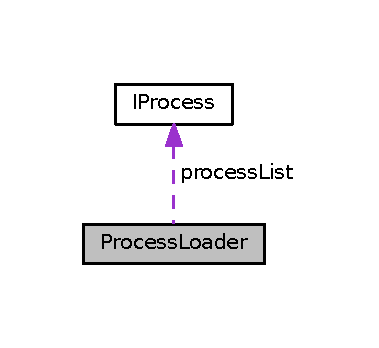
\includegraphics[width=182pt]{classProcessLoader__coll__graph}
\end{center}
\end{figure}
\subsection*{Public Member Functions}
\begin{DoxyCompactItemize}
\item 
\hyperlink{classProcessLoader_ab05abf5a6940a941313b66091993ebca}{Process\+Loader} (C\+Logger \&\hyperlink{classProcessLoader_a46ab766d18e7107c79aa47887013a6ac}{m\+Logger})
\item 
\hyperlink{classProcessLoader_a1c2b6cca84ea0c5716ec505eccae01d8}{$\sim$\+Process\+Loader} ()
\end{DoxyCompactItemize}
\subsection*{Public Attributes}
\begin{DoxyCompactItemize}
\item 
\hyperlink{classIProcess}{I\+Process} $\ast$ \hyperlink{classProcessLoader_a6189a22091af37309df381cade676d51}{process\+List} \mbox{[}3\mbox{]}
\end{DoxyCompactItemize}
\subsection*{Protected Attributes}
\begin{DoxyCompactItemize}
\item 
C\+Logger \& \hyperlink{classProcessLoader_a46ab766d18e7107c79aa47887013a6ac}{m\+Logger}
\end{DoxyCompactItemize}


\subsection{Constructor \& Destructor Documentation}
\index{Process\+Loader@{Process\+Loader}!Process\+Loader@{Process\+Loader}}
\index{Process\+Loader@{Process\+Loader}!Process\+Loader@{Process\+Loader}}
\subsubsection[{\texorpdfstring{Process\+Loader(\+C\+Logger \&m\+Logger)}{ProcessLoader(CLogger &mLogger)}}]{\setlength{\rightskip}{0pt plus 5cm}Process\+Loader\+::\+Process\+Loader (
\begin{DoxyParamCaption}
\item[{C\+Logger \&}]{m\+Logger}
\end{DoxyParamCaption}
)}\hypertarget{classProcessLoader_ab05abf5a6940a941313b66091993ebca}{}\label{classProcessLoader_ab05abf5a6940a941313b66091993ebca}
\index{Process\+Loader@{Process\+Loader}!````~Process\+Loader@{$\sim$\+Process\+Loader}}
\index{````~Process\+Loader@{$\sim$\+Process\+Loader}!Process\+Loader@{Process\+Loader}}
\subsubsection[{\texorpdfstring{$\sim$\+Process\+Loader()}{~ProcessLoader()}}]{\setlength{\rightskip}{0pt plus 5cm}Process\+Loader\+::$\sim$\+Process\+Loader (
\begin{DoxyParamCaption}
{}
\end{DoxyParamCaption}
)\hspace{0.3cm}{\ttfamily [inline]}}\hypertarget{classProcessLoader_a1c2b6cca84ea0c5716ec505eccae01d8}{}\label{classProcessLoader_a1c2b6cca84ea0c5716ec505eccae01d8}


\subsection{Member Data Documentation}
\index{Process\+Loader@{Process\+Loader}!m\+Logger@{m\+Logger}}
\index{m\+Logger@{m\+Logger}!Process\+Loader@{Process\+Loader}}
\subsubsection[{\texorpdfstring{m\+Logger}{mLogger}}]{\setlength{\rightskip}{0pt plus 5cm}C\+Logger\& Process\+Loader\+::m\+Logger\hspace{0.3cm}{\ttfamily [protected]}}\hypertarget{classProcessLoader_a46ab766d18e7107c79aa47887013a6ac}{}\label{classProcessLoader_a46ab766d18e7107c79aa47887013a6ac}
\index{Process\+Loader@{Process\+Loader}!process\+List@{process\+List}}
\index{process\+List@{process\+List}!Process\+Loader@{Process\+Loader}}
\subsubsection[{\texorpdfstring{process\+List}{processList}}]{\setlength{\rightskip}{0pt plus 5cm}{\bf I\+Process}$\ast$ Process\+Loader\+::process\+List\mbox{[}3\mbox{]}}\hypertarget{classProcessLoader_a6189a22091af37309df381cade676d51}{}\label{classProcessLoader_a6189a22091af37309df381cade676d51}


The documentation for this class was generated from the following files\+:\begin{DoxyCompactItemize}
\item 
src/kernel/core/\hyperlink{processloader_8h}{processloader.\+h}\item 
src/kernel/core/\hyperlink{processloader_8cpp}{processloader.\+cpp}\end{DoxyCompactItemize}

\hypertarget{classPseudoPartition}{}\section{Pseudo\+Partition Class Reference}
\label{classPseudoPartition}\index{Pseudo\+Partition@{Pseudo\+Partition}}


{\ttfamily \#include $<$pseudo\+\_\+partition.\+hpp$>$}



Inheritance diagram for Pseudo\+Partition\+:
\nopagebreak
\begin{figure}[H]
\begin{center}
\leavevmode
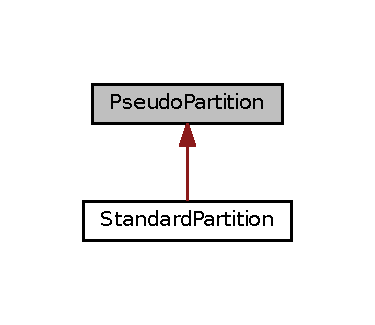
\includegraphics[width=180pt]{classPseudoPartition__inherit__graph}
\end{center}
\end{figure}
\subsection*{Public Member Functions}
\begin{DoxyCompactItemize}
\item 
\hyperlink{classPseudoPartition_a1e3df8b587bbca25afc930951ceea92a}{Pseudo\+Partition} (\hyperlink{structname__t}{name\+\_\+t} name, \hyperlink{general__types_8hpp_a0edc3a86ddf4aa205c6882b61cd7b4e9}{dec\+Or\+Hex\+\_\+t} address, \hyperlink{structname__t}{name\+\_\+t} procedure)
\item 
const std\+::optional$<$ \hyperlink{structname__t}{name\+\_\+t} $>$ \& \hyperlink{classPseudoPartition_afd3c3c1f153ca26e34fb0c8269232fd7}{get\+Name} () const 
\item 
const std\+::optional$<$ \hyperlink{general__types_8hpp_a0edc3a86ddf4aa205c6882b61cd7b4e9}{dec\+Or\+Hex\+\_\+t} $>$ \& \hyperlink{classPseudoPartition_ad6fb3afd813f3a073c4e2f66d7817bd1}{get\+Physical\+Address} () const 
\item 
const std\+::optional$<$ \hyperlink{structname__t}{name\+\_\+t} $>$ \& \hyperlink{classPseudoPartition_a604108a6d3f4437e4def9ad26d94d991}{get\+Procedure} () const 
\end{DoxyCompactItemize}


\subsection{Constructor \& Destructor Documentation}
\index{Pseudo\+Partition@{Pseudo\+Partition}!Pseudo\+Partition@{Pseudo\+Partition}}
\index{Pseudo\+Partition@{Pseudo\+Partition}!Pseudo\+Partition@{Pseudo\+Partition}}
\subsubsection[{\texorpdfstring{Pseudo\+Partition(name\+\_\+t name, dec\+Or\+Hex\+\_\+t address, name\+\_\+t procedure)}{PseudoPartition(name_t name, decOrHex_t address, name_t procedure)}}]{\setlength{\rightskip}{0pt plus 5cm}Pseudo\+Partition\+::\+Pseudo\+Partition (
\begin{DoxyParamCaption}
\item[{{\bf name\+\_\+t}}]{name, }
\item[{{\bf dec\+Or\+Hex\+\_\+t}}]{address, }
\item[{{\bf name\+\_\+t}}]{procedure}
\end{DoxyParamCaption}
)\hspace{0.3cm}{\ttfamily [inline]}}\hypertarget{classPseudoPartition_a1e3df8b587bbca25afc930951ceea92a}{}\label{classPseudoPartition_a1e3df8b587bbca25afc930951ceea92a}


\subsection{Member Function Documentation}
\index{Pseudo\+Partition@{Pseudo\+Partition}!get\+Name@{get\+Name}}
\index{get\+Name@{get\+Name}!Pseudo\+Partition@{Pseudo\+Partition}}
\subsubsection[{\texorpdfstring{get\+Name() const }{getName() const }}]{\setlength{\rightskip}{0pt plus 5cm}const std\+::optional$<$ {\bf name\+\_\+t} $>$ \& Pseudo\+Partition\+::get\+Name (
\begin{DoxyParamCaption}
{}
\end{DoxyParamCaption}
) const}\hypertarget{classPseudoPartition_afd3c3c1f153ca26e34fb0c8269232fd7}{}\label{classPseudoPartition_afd3c3c1f153ca26e34fb0c8269232fd7}
\index{Pseudo\+Partition@{Pseudo\+Partition}!get\+Physical\+Address@{get\+Physical\+Address}}
\index{get\+Physical\+Address@{get\+Physical\+Address}!Pseudo\+Partition@{Pseudo\+Partition}}
\subsubsection[{\texorpdfstring{get\+Physical\+Address() const }{getPhysicalAddress() const }}]{\setlength{\rightskip}{0pt plus 5cm}const std\+::optional$<$ {\bf dec\+Or\+Hex\+\_\+t} $>$ \& Pseudo\+Partition\+::get\+Physical\+Address (
\begin{DoxyParamCaption}
{}
\end{DoxyParamCaption}
) const}\hypertarget{classPseudoPartition_ad6fb3afd813f3a073c4e2f66d7817bd1}{}\label{classPseudoPartition_ad6fb3afd813f3a073c4e2f66d7817bd1}
\index{Pseudo\+Partition@{Pseudo\+Partition}!get\+Procedure@{get\+Procedure}}
\index{get\+Procedure@{get\+Procedure}!Pseudo\+Partition@{Pseudo\+Partition}}
\subsubsection[{\texorpdfstring{get\+Procedure() const }{getProcedure() const }}]{\setlength{\rightskip}{0pt plus 5cm}const std\+::optional$<$ {\bf name\+\_\+t} $>$ \& Pseudo\+Partition\+::get\+Procedure (
\begin{DoxyParamCaption}
{}
\end{DoxyParamCaption}
) const}\hypertarget{classPseudoPartition_a604108a6d3f4437e4def9ad26d94d991}{}\label{classPseudoPartition_a604108a6d3f4437e4def9ad26d94d991}


The documentation for this class was generated from the following files\+:\begin{DoxyCompactItemize}
\item 
src/types/include/\hyperlink{pseudo__partition_8hpp}{pseudo\+\_\+partition.\+hpp}\item 
src/types/src/\hyperlink{pseudo__partition_8cpp}{pseudo\+\_\+partition.\+cpp}\end{DoxyCompactItemize}

\hypertarget{structQUEUING__PORT__STATUS__TYPE}{}\section{Q\+U\+E\+U\+I\+N\+G\+\_\+\+P\+O\+R\+T\+\_\+\+S\+T\+A\+T\+U\+S\+\_\+\+T\+Y\+PE Struct Reference}
\label{structQUEUING__PORT__STATUS__TYPE}\index{Q\+U\+E\+U\+I\+N\+G\+\_\+\+P\+O\+R\+T\+\_\+\+S\+T\+A\+T\+U\+S\+\_\+\+T\+Y\+PE@{Q\+U\+E\+U\+I\+N\+G\+\_\+\+P\+O\+R\+T\+\_\+\+S\+T\+A\+T\+U\+S\+\_\+\+T\+Y\+PE}}


{\ttfamily \#include $<$apex\+\_\+queuing\+\_\+port.\+h$>$}

\subsection*{Public Attributes}
\begin{DoxyCompactItemize}
\item 
\hyperlink{apex__types_8h_aeffd61fe45ce21b94c1f0b5b84e614ea}{M\+E\+S\+S\+A\+G\+E\+\_\+\+R\+A\+N\+G\+E\+\_\+\+T\+Y\+PE} \hyperlink{structQUEUING__PORT__STATUS__TYPE_a205c62d4635ec296b618807a2c099530}{N\+B\+\_\+\+M\+E\+S\+S\+A\+GE}
\item 
\hyperlink{apex__types_8h_aeffd61fe45ce21b94c1f0b5b84e614ea}{M\+E\+S\+S\+A\+G\+E\+\_\+\+R\+A\+N\+G\+E\+\_\+\+T\+Y\+PE} \hyperlink{structQUEUING__PORT__STATUS__TYPE_a801e072e20f37f50eab52bed36647f34}{M\+A\+X\+\_\+\+N\+B\+\_\+\+M\+E\+S\+S\+A\+GE}
\item 
\hyperlink{apex__types_8h_ae09494a8d78c38c94f0cc5a80e69785a}{M\+E\+S\+S\+A\+G\+E\+\_\+\+S\+I\+Z\+E\+\_\+\+T\+Y\+PE} \hyperlink{structQUEUING__PORT__STATUS__TYPE_adac8033102332e5adb686befa554ed48}{M\+A\+X\+\_\+\+M\+E\+S\+S\+A\+G\+E\+\_\+\+S\+I\+ZE}
\item 
\hyperlink{apex__types_8h_ae82fcf2f7f6f7966d59d9569049531a4}{P\+O\+R\+T\+\_\+\+D\+I\+R\+E\+C\+T\+I\+O\+N\+\_\+\+T\+Y\+PE} \hyperlink{structQUEUING__PORT__STATUS__TYPE_af3d8b40327cd03b1397e441441408738}{P\+O\+R\+T\+\_\+\+D\+I\+R\+E\+C\+T\+I\+ON}
\item 
\hyperlink{apex__process_8h_a77a39a661169092676366eec0d65ab1c}{W\+A\+I\+T\+I\+N\+G\+\_\+\+R\+A\+N\+G\+E\+\_\+\+T\+Y\+PE} \hyperlink{structQUEUING__PORT__STATUS__TYPE_a4b68d92cd2d0481a18ba44cfeb6f9e44}{W\+A\+I\+T\+I\+N\+G\+\_\+\+P\+R\+O\+C\+E\+S\+S\+ES}
\end{DoxyCompactItemize}


\subsection{Member Data Documentation}
\index{Q\+U\+E\+U\+I\+N\+G\+\_\+\+P\+O\+R\+T\+\_\+\+S\+T\+A\+T\+U\+S\+\_\+\+T\+Y\+PE@{Q\+U\+E\+U\+I\+N\+G\+\_\+\+P\+O\+R\+T\+\_\+\+S\+T\+A\+T\+U\+S\+\_\+\+T\+Y\+PE}!M\+A\+X\+\_\+\+M\+E\+S\+S\+A\+G\+E\+\_\+\+S\+I\+ZE@{M\+A\+X\+\_\+\+M\+E\+S\+S\+A\+G\+E\+\_\+\+S\+I\+ZE}}
\index{M\+A\+X\+\_\+\+M\+E\+S\+S\+A\+G\+E\+\_\+\+S\+I\+ZE@{M\+A\+X\+\_\+\+M\+E\+S\+S\+A\+G\+E\+\_\+\+S\+I\+ZE}!Q\+U\+E\+U\+I\+N\+G\+\_\+\+P\+O\+R\+T\+\_\+\+S\+T\+A\+T\+U\+S\+\_\+\+T\+Y\+PE@{Q\+U\+E\+U\+I\+N\+G\+\_\+\+P\+O\+R\+T\+\_\+\+S\+T\+A\+T\+U\+S\+\_\+\+T\+Y\+PE}}
\subsubsection[{\texorpdfstring{M\+A\+X\+\_\+\+M\+E\+S\+S\+A\+G\+E\+\_\+\+S\+I\+ZE}{MAX_MESSAGE_SIZE}}]{\setlength{\rightskip}{0pt plus 5cm}{\bf M\+E\+S\+S\+A\+G\+E\+\_\+\+S\+I\+Z\+E\+\_\+\+T\+Y\+PE} Q\+U\+E\+U\+I\+N\+G\+\_\+\+P\+O\+R\+T\+\_\+\+S\+T\+A\+T\+U\+S\+\_\+\+T\+Y\+P\+E\+::\+M\+A\+X\+\_\+\+M\+E\+S\+S\+A\+G\+E\+\_\+\+S\+I\+ZE}\hypertarget{structQUEUING__PORT__STATUS__TYPE_adac8033102332e5adb686befa554ed48}{}\label{structQUEUING__PORT__STATUS__TYPE_adac8033102332e5adb686befa554ed48}
\index{Q\+U\+E\+U\+I\+N\+G\+\_\+\+P\+O\+R\+T\+\_\+\+S\+T\+A\+T\+U\+S\+\_\+\+T\+Y\+PE@{Q\+U\+E\+U\+I\+N\+G\+\_\+\+P\+O\+R\+T\+\_\+\+S\+T\+A\+T\+U\+S\+\_\+\+T\+Y\+PE}!M\+A\+X\+\_\+\+N\+B\+\_\+\+M\+E\+S\+S\+A\+GE@{M\+A\+X\+\_\+\+N\+B\+\_\+\+M\+E\+S\+S\+A\+GE}}
\index{M\+A\+X\+\_\+\+N\+B\+\_\+\+M\+E\+S\+S\+A\+GE@{M\+A\+X\+\_\+\+N\+B\+\_\+\+M\+E\+S\+S\+A\+GE}!Q\+U\+E\+U\+I\+N\+G\+\_\+\+P\+O\+R\+T\+\_\+\+S\+T\+A\+T\+U\+S\+\_\+\+T\+Y\+PE@{Q\+U\+E\+U\+I\+N\+G\+\_\+\+P\+O\+R\+T\+\_\+\+S\+T\+A\+T\+U\+S\+\_\+\+T\+Y\+PE}}
\subsubsection[{\texorpdfstring{M\+A\+X\+\_\+\+N\+B\+\_\+\+M\+E\+S\+S\+A\+GE}{MAX_NB_MESSAGE}}]{\setlength{\rightskip}{0pt plus 5cm}{\bf M\+E\+S\+S\+A\+G\+E\+\_\+\+R\+A\+N\+G\+E\+\_\+\+T\+Y\+PE} Q\+U\+E\+U\+I\+N\+G\+\_\+\+P\+O\+R\+T\+\_\+\+S\+T\+A\+T\+U\+S\+\_\+\+T\+Y\+P\+E\+::\+M\+A\+X\+\_\+\+N\+B\+\_\+\+M\+E\+S\+S\+A\+GE}\hypertarget{structQUEUING__PORT__STATUS__TYPE_a801e072e20f37f50eab52bed36647f34}{}\label{structQUEUING__PORT__STATUS__TYPE_a801e072e20f37f50eab52bed36647f34}
\index{Q\+U\+E\+U\+I\+N\+G\+\_\+\+P\+O\+R\+T\+\_\+\+S\+T\+A\+T\+U\+S\+\_\+\+T\+Y\+PE@{Q\+U\+E\+U\+I\+N\+G\+\_\+\+P\+O\+R\+T\+\_\+\+S\+T\+A\+T\+U\+S\+\_\+\+T\+Y\+PE}!N\+B\+\_\+\+M\+E\+S\+S\+A\+GE@{N\+B\+\_\+\+M\+E\+S\+S\+A\+GE}}
\index{N\+B\+\_\+\+M\+E\+S\+S\+A\+GE@{N\+B\+\_\+\+M\+E\+S\+S\+A\+GE}!Q\+U\+E\+U\+I\+N\+G\+\_\+\+P\+O\+R\+T\+\_\+\+S\+T\+A\+T\+U\+S\+\_\+\+T\+Y\+PE@{Q\+U\+E\+U\+I\+N\+G\+\_\+\+P\+O\+R\+T\+\_\+\+S\+T\+A\+T\+U\+S\+\_\+\+T\+Y\+PE}}
\subsubsection[{\texorpdfstring{N\+B\+\_\+\+M\+E\+S\+S\+A\+GE}{NB_MESSAGE}}]{\setlength{\rightskip}{0pt plus 5cm}{\bf M\+E\+S\+S\+A\+G\+E\+\_\+\+R\+A\+N\+G\+E\+\_\+\+T\+Y\+PE} Q\+U\+E\+U\+I\+N\+G\+\_\+\+P\+O\+R\+T\+\_\+\+S\+T\+A\+T\+U\+S\+\_\+\+T\+Y\+P\+E\+::\+N\+B\+\_\+\+M\+E\+S\+S\+A\+GE}\hypertarget{structQUEUING__PORT__STATUS__TYPE_a205c62d4635ec296b618807a2c099530}{}\label{structQUEUING__PORT__STATUS__TYPE_a205c62d4635ec296b618807a2c099530}
\index{Q\+U\+E\+U\+I\+N\+G\+\_\+\+P\+O\+R\+T\+\_\+\+S\+T\+A\+T\+U\+S\+\_\+\+T\+Y\+PE@{Q\+U\+E\+U\+I\+N\+G\+\_\+\+P\+O\+R\+T\+\_\+\+S\+T\+A\+T\+U\+S\+\_\+\+T\+Y\+PE}!P\+O\+R\+T\+\_\+\+D\+I\+R\+E\+C\+T\+I\+ON@{P\+O\+R\+T\+\_\+\+D\+I\+R\+E\+C\+T\+I\+ON}}
\index{P\+O\+R\+T\+\_\+\+D\+I\+R\+E\+C\+T\+I\+ON@{P\+O\+R\+T\+\_\+\+D\+I\+R\+E\+C\+T\+I\+ON}!Q\+U\+E\+U\+I\+N\+G\+\_\+\+P\+O\+R\+T\+\_\+\+S\+T\+A\+T\+U\+S\+\_\+\+T\+Y\+PE@{Q\+U\+E\+U\+I\+N\+G\+\_\+\+P\+O\+R\+T\+\_\+\+S\+T\+A\+T\+U\+S\+\_\+\+T\+Y\+PE}}
\subsubsection[{\texorpdfstring{P\+O\+R\+T\+\_\+\+D\+I\+R\+E\+C\+T\+I\+ON}{PORT_DIRECTION}}]{\setlength{\rightskip}{0pt plus 5cm}{\bf P\+O\+R\+T\+\_\+\+D\+I\+R\+E\+C\+T\+I\+O\+N\+\_\+\+T\+Y\+PE} Q\+U\+E\+U\+I\+N\+G\+\_\+\+P\+O\+R\+T\+\_\+\+S\+T\+A\+T\+U\+S\+\_\+\+T\+Y\+P\+E\+::\+P\+O\+R\+T\+\_\+\+D\+I\+R\+E\+C\+T\+I\+ON}\hypertarget{structQUEUING__PORT__STATUS__TYPE_af3d8b40327cd03b1397e441441408738}{}\label{structQUEUING__PORT__STATUS__TYPE_af3d8b40327cd03b1397e441441408738}
\index{Q\+U\+E\+U\+I\+N\+G\+\_\+\+P\+O\+R\+T\+\_\+\+S\+T\+A\+T\+U\+S\+\_\+\+T\+Y\+PE@{Q\+U\+E\+U\+I\+N\+G\+\_\+\+P\+O\+R\+T\+\_\+\+S\+T\+A\+T\+U\+S\+\_\+\+T\+Y\+PE}!W\+A\+I\+T\+I\+N\+G\+\_\+\+P\+R\+O\+C\+E\+S\+S\+ES@{W\+A\+I\+T\+I\+N\+G\+\_\+\+P\+R\+O\+C\+E\+S\+S\+ES}}
\index{W\+A\+I\+T\+I\+N\+G\+\_\+\+P\+R\+O\+C\+E\+S\+S\+ES@{W\+A\+I\+T\+I\+N\+G\+\_\+\+P\+R\+O\+C\+E\+S\+S\+ES}!Q\+U\+E\+U\+I\+N\+G\+\_\+\+P\+O\+R\+T\+\_\+\+S\+T\+A\+T\+U\+S\+\_\+\+T\+Y\+PE@{Q\+U\+E\+U\+I\+N\+G\+\_\+\+P\+O\+R\+T\+\_\+\+S\+T\+A\+T\+U\+S\+\_\+\+T\+Y\+PE}}
\subsubsection[{\texorpdfstring{W\+A\+I\+T\+I\+N\+G\+\_\+\+P\+R\+O\+C\+E\+S\+S\+ES}{WAITING_PROCESSES}}]{\setlength{\rightskip}{0pt plus 5cm}{\bf W\+A\+I\+T\+I\+N\+G\+\_\+\+R\+A\+N\+G\+E\+\_\+\+T\+Y\+PE} Q\+U\+E\+U\+I\+N\+G\+\_\+\+P\+O\+R\+T\+\_\+\+S\+T\+A\+T\+U\+S\+\_\+\+T\+Y\+P\+E\+::\+W\+A\+I\+T\+I\+N\+G\+\_\+\+P\+R\+O\+C\+E\+S\+S\+ES}\hypertarget{structQUEUING__PORT__STATUS__TYPE_a4b68d92cd2d0481a18ba44cfeb6f9e44}{}\label{structQUEUING__PORT__STATUS__TYPE_a4b68d92cd2d0481a18ba44cfeb6f9e44}


The documentation for this struct was generated from the following file\+:\begin{DoxyCompactItemize}
\item 
src/libuser/apex/\hyperlink{apex__queuing__port_8h}{apex\+\_\+queuing\+\_\+port.\+h}\end{DoxyCompactItemize}

\hypertarget{classQueuingPort}{}\section{Queuing\+Port Class Reference}
\label{classQueuingPort}\index{Queuing\+Port@{Queuing\+Port}}


{\ttfamily \#include $<$queuing\+\_\+port.\+hpp$>$}



Inheritance diagram for Queuing\+Port\+:\nopagebreak
\begin{figure}[H]
\begin{center}
\leavevmode
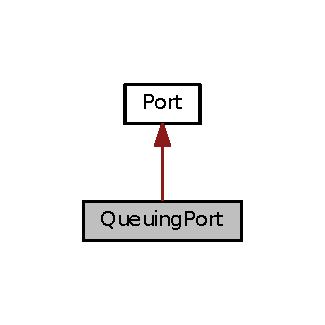
\includegraphics[width=156pt]{classQueuingPort__inherit__graph}
\end{center}
\end{figure}


Collaboration diagram for Queuing\+Port\+:\nopagebreak
\begin{figure}[H]
\begin{center}
\leavevmode
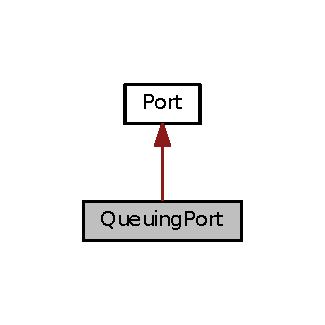
\includegraphics[width=156pt]{classQueuingPort__coll__graph}
\end{center}
\end{figure}
\subsection*{Public Member Functions}
\begin{DoxyCompactItemize}
\item 
\hyperlink{classQueuingPort_a71021f252113f871c481015a4610010e}{Queuing\+Port} ()
\item 
\hyperlink{classQueuingPort_af8f0696eb126e99ac2db4a604555b86e}{Queuing\+Port} (\hyperlink{structname__t}{name\+\_\+t} name, \hyperlink{apex__types_8h_a4e13487a80a5740717e19f7f693e06c3}{A\+P\+E\+X\+\_\+\+I\+N\+T\+E\+G\+ER} msg\+Size, \hyperlink{apex__types_8h_ae82fcf2f7f6f7966d59d9569049531a4}{P\+O\+R\+T\+\_\+\+D\+I\+R\+E\+C\+T\+I\+O\+N\+\_\+\+T\+Y\+PE} direction, \hyperlink{apex__types_8h_a4e13487a80a5740717e19f7f693e06c3}{A\+P\+E\+X\+\_\+\+I\+N\+T\+E\+G\+ER} max\+Messages)
\item 
const \hyperlink{apex__types_8h_a4e13487a80a5740717e19f7f693e06c3}{A\+P\+E\+X\+\_\+\+I\+N\+T\+E\+G\+ER} \& \hyperlink{classQueuingPort_a8f23ad43267728c7ecbd0ee1dd2edb6f}{get\+Max\+Num\+Messages} () const 
\end{DoxyCompactItemize}


\subsection{Constructor \& Destructor Documentation}
\index{Queuing\+Port@{Queuing\+Port}!Queuing\+Port@{Queuing\+Port}}
\index{Queuing\+Port@{Queuing\+Port}!Queuing\+Port@{Queuing\+Port}}
\subsubsection[{\texorpdfstring{Queuing\+Port()}{QueuingPort()}}]{\setlength{\rightskip}{0pt plus 5cm}Queuing\+Port\+::\+Queuing\+Port (
\begin{DoxyParamCaption}
{}
\end{DoxyParamCaption}
)\hspace{0.3cm}{\ttfamily [inline]}}\hypertarget{classQueuingPort_a71021f252113f871c481015a4610010e}{}\label{classQueuingPort_a71021f252113f871c481015a4610010e}
\index{Queuing\+Port@{Queuing\+Port}!Queuing\+Port@{Queuing\+Port}}
\index{Queuing\+Port@{Queuing\+Port}!Queuing\+Port@{Queuing\+Port}}
\subsubsection[{\texorpdfstring{Queuing\+Port(name\+\_\+t name, A\+P\+E\+X\+\_\+\+I\+N\+T\+E\+G\+E\+R msg\+Size, P\+O\+R\+T\+\_\+\+D\+I\+R\+E\+C\+T\+I\+O\+N\+\_\+\+T\+Y\+P\+E direction, A\+P\+E\+X\+\_\+\+I\+N\+T\+E\+G\+E\+R max\+Messages)}{QueuingPort(name_t name, APEX_INTEGER msgSize, PORT_DIRECTION_TYPE direction, APEX_INTEGER maxMessages)}}]{\setlength{\rightskip}{0pt plus 5cm}Queuing\+Port\+::\+Queuing\+Port (
\begin{DoxyParamCaption}
\item[{{\bf name\+\_\+t}}]{name, }
\item[{{\bf A\+P\+E\+X\+\_\+\+I\+N\+T\+E\+G\+ER}}]{msg\+Size, }
\item[{{\bf P\+O\+R\+T\+\_\+\+D\+I\+R\+E\+C\+T\+I\+O\+N\+\_\+\+T\+Y\+PE}}]{direction, }
\item[{{\bf A\+P\+E\+X\+\_\+\+I\+N\+T\+E\+G\+ER}}]{max\+Messages}
\end{DoxyParamCaption}
)\hspace{0.3cm}{\ttfamily [inline]}}\hypertarget{classQueuingPort_af8f0696eb126e99ac2db4a604555b86e}{}\label{classQueuingPort_af8f0696eb126e99ac2db4a604555b86e}


\subsection{Member Function Documentation}
\index{Queuing\+Port@{Queuing\+Port}!get\+Max\+Num\+Messages@{get\+Max\+Num\+Messages}}
\index{get\+Max\+Num\+Messages@{get\+Max\+Num\+Messages}!Queuing\+Port@{Queuing\+Port}}
\subsubsection[{\texorpdfstring{get\+Max\+Num\+Messages() const }{getMaxNumMessages() const }}]{\setlength{\rightskip}{0pt plus 5cm}const {\bf A\+P\+E\+X\+\_\+\+I\+N\+T\+E\+G\+ER} \& Queuing\+Port\+::get\+Max\+Num\+Messages (
\begin{DoxyParamCaption}
{}
\end{DoxyParamCaption}
) const}\hypertarget{classQueuingPort_a8f23ad43267728c7ecbd0ee1dd2edb6f}{}\label{classQueuingPort_a8f23ad43267728c7ecbd0ee1dd2edb6f}


The documentation for this class was generated from the following files\+:\begin{DoxyCompactItemize}
\item 
src/types/include/\hyperlink{queuing__port_8hpp}{queuing\+\_\+port.\+hpp}\item 
src/types/src/\hyperlink{queuing__port_8cpp}{queuing\+\_\+port.\+cpp}\end{DoxyCompactItemize}

\hypertarget{structSAMPLING__PORT__STATUS__TYPE}{}\section{S\+A\+M\+P\+L\+I\+N\+G\+\_\+\+P\+O\+R\+T\+\_\+\+S\+T\+A\+T\+U\+S\+\_\+\+T\+Y\+PE Struct Reference}
\label{structSAMPLING__PORT__STATUS__TYPE}\index{S\+A\+M\+P\+L\+I\+N\+G\+\_\+\+P\+O\+R\+T\+\_\+\+S\+T\+A\+T\+U\+S\+\_\+\+T\+Y\+PE@{S\+A\+M\+P\+L\+I\+N\+G\+\_\+\+P\+O\+R\+T\+\_\+\+S\+T\+A\+T\+U\+S\+\_\+\+T\+Y\+PE}}


{\ttfamily \#include $<$apex\+\_\+sampling\+\_\+port.\+h$>$}

\subsection*{Public Attributes}
\begin{DoxyCompactItemize}
\item 
\hyperlink{apex__types_8h_a78cd52c2621ddf2eda68fcd4bedbc1a7}{S\+Y\+S\+T\+E\+M\+\_\+\+T\+I\+M\+E\+\_\+\+T\+Y\+PE} \hyperlink{structSAMPLING__PORT__STATUS__TYPE_af01743f2cd919f7d8198a758160f3e58}{R\+E\+F\+R\+E\+S\+H\+\_\+\+P\+E\+R\+I\+OD}
\item 
\hyperlink{apex__types_8h_ae09494a8d78c38c94f0cc5a80e69785a}{M\+E\+S\+S\+A\+G\+E\+\_\+\+S\+I\+Z\+E\+\_\+\+T\+Y\+PE} \hyperlink{structSAMPLING__PORT__STATUS__TYPE_ae49173e0a2e3f323ec8efdeea883971d}{M\+A\+X\+\_\+\+M\+E\+S\+S\+A\+G\+E\+\_\+\+S\+I\+ZE}
\item 
\hyperlink{apex__types_8h_ae82fcf2f7f6f7966d59d9569049531a4}{P\+O\+R\+T\+\_\+\+D\+I\+R\+E\+C\+T\+I\+O\+N\+\_\+\+T\+Y\+PE} \hyperlink{structSAMPLING__PORT__STATUS__TYPE_ae9fbcccaa93fd7f7c811a4e8374933af}{P\+O\+R\+T\+\_\+\+D\+I\+R\+E\+C\+T\+I\+ON}
\item 
\hyperlink{apex__sampling__port_8h_a00855980da372cfa6572e3e3f57ef499}{V\+A\+L\+I\+D\+I\+T\+Y\+\_\+\+T\+Y\+PE} \hyperlink{structSAMPLING__PORT__STATUS__TYPE_ab1b26afc9953625980d046f415ed6d23}{L\+A\+S\+T\+\_\+\+M\+S\+G\+\_\+\+V\+A\+L\+I\+D\+I\+TY}
\end{DoxyCompactItemize}


\subsection{Member Data Documentation}
\index{S\+A\+M\+P\+L\+I\+N\+G\+\_\+\+P\+O\+R\+T\+\_\+\+S\+T\+A\+T\+U\+S\+\_\+\+T\+Y\+PE@{S\+A\+M\+P\+L\+I\+N\+G\+\_\+\+P\+O\+R\+T\+\_\+\+S\+T\+A\+T\+U\+S\+\_\+\+T\+Y\+PE}!L\+A\+S\+T\+\_\+\+M\+S\+G\+\_\+\+V\+A\+L\+I\+D\+I\+TY@{L\+A\+S\+T\+\_\+\+M\+S\+G\+\_\+\+V\+A\+L\+I\+D\+I\+TY}}
\index{L\+A\+S\+T\+\_\+\+M\+S\+G\+\_\+\+V\+A\+L\+I\+D\+I\+TY@{L\+A\+S\+T\+\_\+\+M\+S\+G\+\_\+\+V\+A\+L\+I\+D\+I\+TY}!S\+A\+M\+P\+L\+I\+N\+G\+\_\+\+P\+O\+R\+T\+\_\+\+S\+T\+A\+T\+U\+S\+\_\+\+T\+Y\+PE@{S\+A\+M\+P\+L\+I\+N\+G\+\_\+\+P\+O\+R\+T\+\_\+\+S\+T\+A\+T\+U\+S\+\_\+\+T\+Y\+PE}}
\subsubsection[{\texorpdfstring{L\+A\+S\+T\+\_\+\+M\+S\+G\+\_\+\+V\+A\+L\+I\+D\+I\+TY}{LAST_MSG_VALIDITY}}]{\setlength{\rightskip}{0pt plus 5cm}{\bf V\+A\+L\+I\+D\+I\+T\+Y\+\_\+\+T\+Y\+PE} S\+A\+M\+P\+L\+I\+N\+G\+\_\+\+P\+O\+R\+T\+\_\+\+S\+T\+A\+T\+U\+S\+\_\+\+T\+Y\+P\+E\+::\+L\+A\+S\+T\+\_\+\+M\+S\+G\+\_\+\+V\+A\+L\+I\+D\+I\+TY}\hypertarget{structSAMPLING__PORT__STATUS__TYPE_ab1b26afc9953625980d046f415ed6d23}{}\label{structSAMPLING__PORT__STATUS__TYPE_ab1b26afc9953625980d046f415ed6d23}
\index{S\+A\+M\+P\+L\+I\+N\+G\+\_\+\+P\+O\+R\+T\+\_\+\+S\+T\+A\+T\+U\+S\+\_\+\+T\+Y\+PE@{S\+A\+M\+P\+L\+I\+N\+G\+\_\+\+P\+O\+R\+T\+\_\+\+S\+T\+A\+T\+U\+S\+\_\+\+T\+Y\+PE}!M\+A\+X\+\_\+\+M\+E\+S\+S\+A\+G\+E\+\_\+\+S\+I\+ZE@{M\+A\+X\+\_\+\+M\+E\+S\+S\+A\+G\+E\+\_\+\+S\+I\+ZE}}
\index{M\+A\+X\+\_\+\+M\+E\+S\+S\+A\+G\+E\+\_\+\+S\+I\+ZE@{M\+A\+X\+\_\+\+M\+E\+S\+S\+A\+G\+E\+\_\+\+S\+I\+ZE}!S\+A\+M\+P\+L\+I\+N\+G\+\_\+\+P\+O\+R\+T\+\_\+\+S\+T\+A\+T\+U\+S\+\_\+\+T\+Y\+PE@{S\+A\+M\+P\+L\+I\+N\+G\+\_\+\+P\+O\+R\+T\+\_\+\+S\+T\+A\+T\+U\+S\+\_\+\+T\+Y\+PE}}
\subsubsection[{\texorpdfstring{M\+A\+X\+\_\+\+M\+E\+S\+S\+A\+G\+E\+\_\+\+S\+I\+ZE}{MAX_MESSAGE_SIZE}}]{\setlength{\rightskip}{0pt plus 5cm}{\bf M\+E\+S\+S\+A\+G\+E\+\_\+\+S\+I\+Z\+E\+\_\+\+T\+Y\+PE} S\+A\+M\+P\+L\+I\+N\+G\+\_\+\+P\+O\+R\+T\+\_\+\+S\+T\+A\+T\+U\+S\+\_\+\+T\+Y\+P\+E\+::\+M\+A\+X\+\_\+\+M\+E\+S\+S\+A\+G\+E\+\_\+\+S\+I\+ZE}\hypertarget{structSAMPLING__PORT__STATUS__TYPE_ae49173e0a2e3f323ec8efdeea883971d}{}\label{structSAMPLING__PORT__STATUS__TYPE_ae49173e0a2e3f323ec8efdeea883971d}
\index{S\+A\+M\+P\+L\+I\+N\+G\+\_\+\+P\+O\+R\+T\+\_\+\+S\+T\+A\+T\+U\+S\+\_\+\+T\+Y\+PE@{S\+A\+M\+P\+L\+I\+N\+G\+\_\+\+P\+O\+R\+T\+\_\+\+S\+T\+A\+T\+U\+S\+\_\+\+T\+Y\+PE}!P\+O\+R\+T\+\_\+\+D\+I\+R\+E\+C\+T\+I\+ON@{P\+O\+R\+T\+\_\+\+D\+I\+R\+E\+C\+T\+I\+ON}}
\index{P\+O\+R\+T\+\_\+\+D\+I\+R\+E\+C\+T\+I\+ON@{P\+O\+R\+T\+\_\+\+D\+I\+R\+E\+C\+T\+I\+ON}!S\+A\+M\+P\+L\+I\+N\+G\+\_\+\+P\+O\+R\+T\+\_\+\+S\+T\+A\+T\+U\+S\+\_\+\+T\+Y\+PE@{S\+A\+M\+P\+L\+I\+N\+G\+\_\+\+P\+O\+R\+T\+\_\+\+S\+T\+A\+T\+U\+S\+\_\+\+T\+Y\+PE}}
\subsubsection[{\texorpdfstring{P\+O\+R\+T\+\_\+\+D\+I\+R\+E\+C\+T\+I\+ON}{PORT_DIRECTION}}]{\setlength{\rightskip}{0pt plus 5cm}{\bf P\+O\+R\+T\+\_\+\+D\+I\+R\+E\+C\+T\+I\+O\+N\+\_\+\+T\+Y\+PE} S\+A\+M\+P\+L\+I\+N\+G\+\_\+\+P\+O\+R\+T\+\_\+\+S\+T\+A\+T\+U\+S\+\_\+\+T\+Y\+P\+E\+::\+P\+O\+R\+T\+\_\+\+D\+I\+R\+E\+C\+T\+I\+ON}\hypertarget{structSAMPLING__PORT__STATUS__TYPE_ae9fbcccaa93fd7f7c811a4e8374933af}{}\label{structSAMPLING__PORT__STATUS__TYPE_ae9fbcccaa93fd7f7c811a4e8374933af}
\index{S\+A\+M\+P\+L\+I\+N\+G\+\_\+\+P\+O\+R\+T\+\_\+\+S\+T\+A\+T\+U\+S\+\_\+\+T\+Y\+PE@{S\+A\+M\+P\+L\+I\+N\+G\+\_\+\+P\+O\+R\+T\+\_\+\+S\+T\+A\+T\+U\+S\+\_\+\+T\+Y\+PE}!R\+E\+F\+R\+E\+S\+H\+\_\+\+P\+E\+R\+I\+OD@{R\+E\+F\+R\+E\+S\+H\+\_\+\+P\+E\+R\+I\+OD}}
\index{R\+E\+F\+R\+E\+S\+H\+\_\+\+P\+E\+R\+I\+OD@{R\+E\+F\+R\+E\+S\+H\+\_\+\+P\+E\+R\+I\+OD}!S\+A\+M\+P\+L\+I\+N\+G\+\_\+\+P\+O\+R\+T\+\_\+\+S\+T\+A\+T\+U\+S\+\_\+\+T\+Y\+PE@{S\+A\+M\+P\+L\+I\+N\+G\+\_\+\+P\+O\+R\+T\+\_\+\+S\+T\+A\+T\+U\+S\+\_\+\+T\+Y\+PE}}
\subsubsection[{\texorpdfstring{R\+E\+F\+R\+E\+S\+H\+\_\+\+P\+E\+R\+I\+OD}{REFRESH_PERIOD}}]{\setlength{\rightskip}{0pt plus 5cm}{\bf S\+Y\+S\+T\+E\+M\+\_\+\+T\+I\+M\+E\+\_\+\+T\+Y\+PE} S\+A\+M\+P\+L\+I\+N\+G\+\_\+\+P\+O\+R\+T\+\_\+\+S\+T\+A\+T\+U\+S\+\_\+\+T\+Y\+P\+E\+::\+R\+E\+F\+R\+E\+S\+H\+\_\+\+P\+E\+R\+I\+OD}\hypertarget{structSAMPLING__PORT__STATUS__TYPE_af01743f2cd919f7d8198a758160f3e58}{}\label{structSAMPLING__PORT__STATUS__TYPE_af01743f2cd919f7d8198a758160f3e58}


The documentation for this struct was generated from the following file\+:\begin{DoxyCompactItemize}
\item 
src/libuser/apex/\hyperlink{apex__sampling__port_8h}{apex\+\_\+sampling\+\_\+port.\+h}\end{DoxyCompactItemize}

\hypertarget{classSamplingPort}{}\section{Sampling\+Port Class Reference}
\label{classSamplingPort}\index{Sampling\+Port@{Sampling\+Port}}


{\ttfamily \#include $<$sampling\+\_\+port.\+hpp$>$}



Inheritance diagram for Sampling\+Port\+:
\nopagebreak
\begin{figure}[H]
\begin{center}
\leavevmode
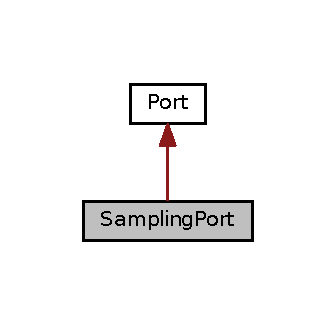
\includegraphics[width=161pt]{classSamplingPort__inherit__graph}
\end{center}
\end{figure}


Collaboration diagram for Sampling\+Port\+:
\nopagebreak
\begin{figure}[H]
\begin{center}
\leavevmode
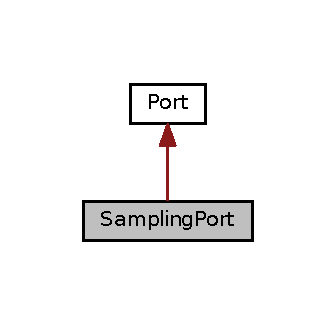
\includegraphics[width=161pt]{classSamplingPort__coll__graph}
\end{center}
\end{figure}
\subsection*{Public Member Functions}
\begin{DoxyCompactItemize}
\item 
\hyperlink{classSamplingPort_a493e0b37d7593294878395ba45c27b09}{Sampling\+Port} ()
\item 
\hyperlink{classSamplingPort_a7318dd4e9c66334d6bb4607b7d464641}{Sampling\+Port} (\hyperlink{structname__t}{name\+\_\+t} name, \hyperlink{apex__types_8h_a4e13487a80a5740717e19f7f693e06c3}{A\+P\+E\+X\+\_\+\+I\+N\+T\+E\+G\+ER} msg\+Size, \hyperlink{apex__types_8h_ae82fcf2f7f6f7966d59d9569049531a4}{P\+O\+R\+T\+\_\+\+D\+I\+R\+E\+C\+T\+I\+O\+N\+\_\+\+T\+Y\+PE} direction, float refresh\+Rate)
\item 
const std\+::optional$<$ float $>$ \& \hyperlink{classSamplingPort_a3601c9fe8b8f15f6c7af956d30bc37df}{get\+Refresh\+Rate} () const 
\end{DoxyCompactItemize}


\subsection{Constructor \& Destructor Documentation}
\index{Sampling\+Port@{Sampling\+Port}!Sampling\+Port@{Sampling\+Port}}
\index{Sampling\+Port@{Sampling\+Port}!Sampling\+Port@{Sampling\+Port}}
\subsubsection[{\texorpdfstring{Sampling\+Port()}{SamplingPort()}}]{\setlength{\rightskip}{0pt plus 5cm}Sampling\+Port\+::\+Sampling\+Port (
\begin{DoxyParamCaption}
{}
\end{DoxyParamCaption}
)\hspace{0.3cm}{\ttfamily [inline]}}\hypertarget{classSamplingPort_a493e0b37d7593294878395ba45c27b09}{}\label{classSamplingPort_a493e0b37d7593294878395ba45c27b09}
\index{Sampling\+Port@{Sampling\+Port}!Sampling\+Port@{Sampling\+Port}}
\index{Sampling\+Port@{Sampling\+Port}!Sampling\+Port@{Sampling\+Port}}
\subsubsection[{\texorpdfstring{Sampling\+Port(name\+\_\+t name, A\+P\+E\+X\+\_\+\+I\+N\+T\+E\+G\+E\+R msg\+Size, P\+O\+R\+T\+\_\+\+D\+I\+R\+E\+C\+T\+I\+O\+N\+\_\+\+T\+Y\+P\+E direction, float refresh\+Rate)}{SamplingPort(name_t name, APEX_INTEGER msgSize, PORT_DIRECTION_TYPE direction, float refreshRate)}}]{\setlength{\rightskip}{0pt plus 5cm}Sampling\+Port\+::\+Sampling\+Port (
\begin{DoxyParamCaption}
\item[{{\bf name\+\_\+t}}]{name, }
\item[{{\bf A\+P\+E\+X\+\_\+\+I\+N\+T\+E\+G\+ER}}]{msg\+Size, }
\item[{{\bf P\+O\+R\+T\+\_\+\+D\+I\+R\+E\+C\+T\+I\+O\+N\+\_\+\+T\+Y\+PE}}]{direction, }
\item[{float}]{refresh\+Rate}
\end{DoxyParamCaption}
)\hspace{0.3cm}{\ttfamily [inline]}}\hypertarget{classSamplingPort_a7318dd4e9c66334d6bb4607b7d464641}{}\label{classSamplingPort_a7318dd4e9c66334d6bb4607b7d464641}


\subsection{Member Function Documentation}
\index{Sampling\+Port@{Sampling\+Port}!get\+Refresh\+Rate@{get\+Refresh\+Rate}}
\index{get\+Refresh\+Rate@{get\+Refresh\+Rate}!Sampling\+Port@{Sampling\+Port}}
\subsubsection[{\texorpdfstring{get\+Refresh\+Rate() const }{getRefreshRate() const }}]{\setlength{\rightskip}{0pt plus 5cm}const std\+::optional$<$ float $>$ \& Sampling\+Port\+::get\+Refresh\+Rate (
\begin{DoxyParamCaption}
{}
\end{DoxyParamCaption}
) const}\hypertarget{classSamplingPort_a3601c9fe8b8f15f6c7af956d30bc37df}{}\label{classSamplingPort_a3601c9fe8b8f15f6c7af956d30bc37df}


The documentation for this class was generated from the following files\+:\begin{DoxyCompactItemize}
\item 
src/types/include/\hyperlink{sampling__port_8hpp}{sampling\+\_\+port.\+hpp}\item 
src/types/src/\hyperlink{sampling__port_8cpp}{sampling\+\_\+port.\+cpp}\end{DoxyCompactItemize}

\hypertarget{structSEMAPHORE__STATUS__TYPE}{}\section{S\+E\+M\+A\+P\+H\+O\+R\+E\+\_\+\+S\+T\+A\+T\+U\+S\+\_\+\+T\+Y\+PE Struct Reference}
\label{structSEMAPHORE__STATUS__TYPE}\index{S\+E\+M\+A\+P\+H\+O\+R\+E\+\_\+\+S\+T\+A\+T\+U\+S\+\_\+\+T\+Y\+PE@{S\+E\+M\+A\+P\+H\+O\+R\+E\+\_\+\+S\+T\+A\+T\+U\+S\+\_\+\+T\+Y\+PE}}


{\ttfamily \#include $<$apex\+\_\+semaphore.\+h$>$}

\subsection*{Public Attributes}
\begin{DoxyCompactItemize}
\item 
\hyperlink{apex__semaphore_8h_a6a4f4a98d5659e166b13ded30fd03d8e}{S\+E\+M\+A\+P\+H\+O\+R\+E\+\_\+\+V\+A\+L\+U\+E\+\_\+\+T\+Y\+PE} \hyperlink{structSEMAPHORE__STATUS__TYPE_a9bc5c320be2f437679f9ce1b0a3037c2}{C\+U\+R\+R\+E\+N\+T\+\_\+\+V\+A\+L\+UE}
\item 
\hyperlink{apex__semaphore_8h_a6a4f4a98d5659e166b13ded30fd03d8e}{S\+E\+M\+A\+P\+H\+O\+R\+E\+\_\+\+V\+A\+L\+U\+E\+\_\+\+T\+Y\+PE} \hyperlink{structSEMAPHORE__STATUS__TYPE_a11b9250a6a0f09b0db3a46c506fc3a5f}{M\+A\+X\+I\+M\+U\+M\+\_\+\+V\+A\+L\+UE}
\item 
\hyperlink{apex__process_8h_a77a39a661169092676366eec0d65ab1c}{W\+A\+I\+T\+I\+N\+G\+\_\+\+R\+A\+N\+G\+E\+\_\+\+T\+Y\+PE} \hyperlink{structSEMAPHORE__STATUS__TYPE_a0fde4e667b650c5ca565b245187ab652}{W\+A\+I\+T\+I\+N\+G\+\_\+\+P\+R\+O\+C\+E\+S\+S\+ES}
\end{DoxyCompactItemize}


\subsection{Member Data Documentation}
\index{S\+E\+M\+A\+P\+H\+O\+R\+E\+\_\+\+S\+T\+A\+T\+U\+S\+\_\+\+T\+Y\+PE@{S\+E\+M\+A\+P\+H\+O\+R\+E\+\_\+\+S\+T\+A\+T\+U\+S\+\_\+\+T\+Y\+PE}!C\+U\+R\+R\+E\+N\+T\+\_\+\+V\+A\+L\+UE@{C\+U\+R\+R\+E\+N\+T\+\_\+\+V\+A\+L\+UE}}
\index{C\+U\+R\+R\+E\+N\+T\+\_\+\+V\+A\+L\+UE@{C\+U\+R\+R\+E\+N\+T\+\_\+\+V\+A\+L\+UE}!S\+E\+M\+A\+P\+H\+O\+R\+E\+\_\+\+S\+T\+A\+T\+U\+S\+\_\+\+T\+Y\+PE@{S\+E\+M\+A\+P\+H\+O\+R\+E\+\_\+\+S\+T\+A\+T\+U\+S\+\_\+\+T\+Y\+PE}}
\subsubsection[{\texorpdfstring{C\+U\+R\+R\+E\+N\+T\+\_\+\+V\+A\+L\+UE}{CURRENT_VALUE}}]{\setlength{\rightskip}{0pt plus 5cm}{\bf S\+E\+M\+A\+P\+H\+O\+R\+E\+\_\+\+V\+A\+L\+U\+E\+\_\+\+T\+Y\+PE} S\+E\+M\+A\+P\+H\+O\+R\+E\+\_\+\+S\+T\+A\+T\+U\+S\+\_\+\+T\+Y\+P\+E\+::\+C\+U\+R\+R\+E\+N\+T\+\_\+\+V\+A\+L\+UE}\hypertarget{structSEMAPHORE__STATUS__TYPE_a9bc5c320be2f437679f9ce1b0a3037c2}{}\label{structSEMAPHORE__STATUS__TYPE_a9bc5c320be2f437679f9ce1b0a3037c2}
\index{S\+E\+M\+A\+P\+H\+O\+R\+E\+\_\+\+S\+T\+A\+T\+U\+S\+\_\+\+T\+Y\+PE@{S\+E\+M\+A\+P\+H\+O\+R\+E\+\_\+\+S\+T\+A\+T\+U\+S\+\_\+\+T\+Y\+PE}!M\+A\+X\+I\+M\+U\+M\+\_\+\+V\+A\+L\+UE@{M\+A\+X\+I\+M\+U\+M\+\_\+\+V\+A\+L\+UE}}
\index{M\+A\+X\+I\+M\+U\+M\+\_\+\+V\+A\+L\+UE@{M\+A\+X\+I\+M\+U\+M\+\_\+\+V\+A\+L\+UE}!S\+E\+M\+A\+P\+H\+O\+R\+E\+\_\+\+S\+T\+A\+T\+U\+S\+\_\+\+T\+Y\+PE@{S\+E\+M\+A\+P\+H\+O\+R\+E\+\_\+\+S\+T\+A\+T\+U\+S\+\_\+\+T\+Y\+PE}}
\subsubsection[{\texorpdfstring{M\+A\+X\+I\+M\+U\+M\+\_\+\+V\+A\+L\+UE}{MAXIMUM_VALUE}}]{\setlength{\rightskip}{0pt plus 5cm}{\bf S\+E\+M\+A\+P\+H\+O\+R\+E\+\_\+\+V\+A\+L\+U\+E\+\_\+\+T\+Y\+PE} S\+E\+M\+A\+P\+H\+O\+R\+E\+\_\+\+S\+T\+A\+T\+U\+S\+\_\+\+T\+Y\+P\+E\+::\+M\+A\+X\+I\+M\+U\+M\+\_\+\+V\+A\+L\+UE}\hypertarget{structSEMAPHORE__STATUS__TYPE_a11b9250a6a0f09b0db3a46c506fc3a5f}{}\label{structSEMAPHORE__STATUS__TYPE_a11b9250a6a0f09b0db3a46c506fc3a5f}
\index{S\+E\+M\+A\+P\+H\+O\+R\+E\+\_\+\+S\+T\+A\+T\+U\+S\+\_\+\+T\+Y\+PE@{S\+E\+M\+A\+P\+H\+O\+R\+E\+\_\+\+S\+T\+A\+T\+U\+S\+\_\+\+T\+Y\+PE}!W\+A\+I\+T\+I\+N\+G\+\_\+\+P\+R\+O\+C\+E\+S\+S\+ES@{W\+A\+I\+T\+I\+N\+G\+\_\+\+P\+R\+O\+C\+E\+S\+S\+ES}}
\index{W\+A\+I\+T\+I\+N\+G\+\_\+\+P\+R\+O\+C\+E\+S\+S\+ES@{W\+A\+I\+T\+I\+N\+G\+\_\+\+P\+R\+O\+C\+E\+S\+S\+ES}!S\+E\+M\+A\+P\+H\+O\+R\+E\+\_\+\+S\+T\+A\+T\+U\+S\+\_\+\+T\+Y\+PE@{S\+E\+M\+A\+P\+H\+O\+R\+E\+\_\+\+S\+T\+A\+T\+U\+S\+\_\+\+T\+Y\+PE}}
\subsubsection[{\texorpdfstring{W\+A\+I\+T\+I\+N\+G\+\_\+\+P\+R\+O\+C\+E\+S\+S\+ES}{WAITING_PROCESSES}}]{\setlength{\rightskip}{0pt plus 5cm}{\bf W\+A\+I\+T\+I\+N\+G\+\_\+\+R\+A\+N\+G\+E\+\_\+\+T\+Y\+PE} S\+E\+M\+A\+P\+H\+O\+R\+E\+\_\+\+S\+T\+A\+T\+U\+S\+\_\+\+T\+Y\+P\+E\+::\+W\+A\+I\+T\+I\+N\+G\+\_\+\+P\+R\+O\+C\+E\+S\+S\+ES}\hypertarget{structSEMAPHORE__STATUS__TYPE_a0fde4e667b650c5ca565b245187ab652}{}\label{structSEMAPHORE__STATUS__TYPE_a0fde4e667b650c5ca565b245187ab652}


The documentation for this struct was generated from the following file\+:\begin{DoxyCompactItemize}
\item 
src/libuser/apex/\hyperlink{apex__semaphore_8h}{apex\+\_\+semaphore.\+h}\end{DoxyCompactItemize}

\hypertarget{classStandardPartition}{}\section{Standard\+Partition Class Reference}
\label{classStandardPartition}\index{Standard\+Partition@{Standard\+Partition}}


{\ttfamily \#include $<$standard\+\_\+partition.\+hpp$>$}



Inheritance diagram for Standard\+Partition\+:
\nopagebreak
\begin{figure}[H]
\begin{center}
\leavevmode
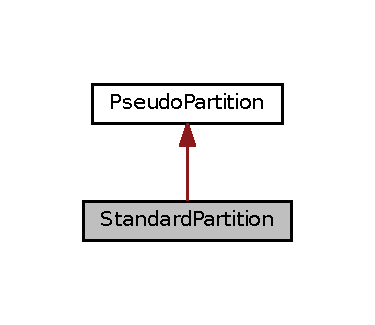
\includegraphics[width=180pt]{classStandardPartition__inherit__graph}
\end{center}
\end{figure}


Collaboration diagram for Standard\+Partition\+:
\nopagebreak
\begin{figure}[H]
\begin{center}
\leavevmode
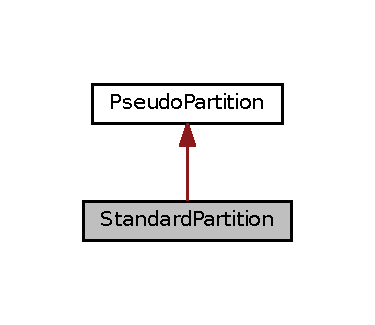
\includegraphics[width=180pt]{classStandardPartition__coll__graph}
\end{center}
\end{figure}
\subsection*{Public Member Functions}
\begin{DoxyCompactItemize}
\item 
\hyperlink{classStandardPartition_ab199d2d1cc720e918d297e04e0cf15c7}{Standard\+Partition} (\hyperlink{general__types_8hpp_a824b78b06da8112c2772bc666a63638d}{identifier\+\_\+t} id, \hyperlink{structname__t}{name\+\_\+t} partition\+Name, \hyperlink{structname__t}{name\+\_\+t} port\+Name, \hyperlink{apex__types_8h_a4e13487a80a5740717e19f7f693e06c3}{A\+P\+E\+X\+\_\+\+I\+N\+T\+E\+G\+ER} address, \hyperlink{structname__t}{name\+\_\+t} procedure)
\item 
const \hyperlink{general__types_8hpp_a824b78b06da8112c2772bc666a63638d}{identifier\+\_\+t} \& \hyperlink{classStandardPartition_ae6b0558f4a415d8c5237d5545b436761}{get\+Partition\+Identifier} () const 
\item 
const \hyperlink{structname__t}{name\+\_\+t} \& \hyperlink{classStandardPartition_a902c2894e54f814ddba69fed047c63c6}{get\+Port\+Name} () const 
\end{DoxyCompactItemize}


\subsection{Constructor \& Destructor Documentation}
\index{Standard\+Partition@{Standard\+Partition}!Standard\+Partition@{Standard\+Partition}}
\index{Standard\+Partition@{Standard\+Partition}!Standard\+Partition@{Standard\+Partition}}
\subsubsection[{\texorpdfstring{Standard\+Partition(identifier\+\_\+t id, name\+\_\+t partition\+Name, name\+\_\+t port\+Name, A\+P\+E\+X\+\_\+\+I\+N\+T\+E\+G\+E\+R address, name\+\_\+t procedure)}{StandardPartition(identifier_t id, name_t partitionName, name_t portName, APEX_INTEGER address, name_t procedure)}}]{\setlength{\rightskip}{0pt plus 5cm}Standard\+Partition\+::\+Standard\+Partition (
\begin{DoxyParamCaption}
\item[{{\bf identifier\+\_\+t}}]{id, }
\item[{{\bf name\+\_\+t}}]{partition\+Name, }
\item[{{\bf name\+\_\+t}}]{port\+Name, }
\item[{{\bf A\+P\+E\+X\+\_\+\+I\+N\+T\+E\+G\+ER}}]{address, }
\item[{{\bf name\+\_\+t}}]{procedure}
\end{DoxyParamCaption}
)\hspace{0.3cm}{\ttfamily [inline]}}\hypertarget{classStandardPartition_ab199d2d1cc720e918d297e04e0cf15c7}{}\label{classStandardPartition_ab199d2d1cc720e918d297e04e0cf15c7}


\subsection{Member Function Documentation}
\index{Standard\+Partition@{Standard\+Partition}!get\+Partition\+Identifier@{get\+Partition\+Identifier}}
\index{get\+Partition\+Identifier@{get\+Partition\+Identifier}!Standard\+Partition@{Standard\+Partition}}
\subsubsection[{\texorpdfstring{get\+Partition\+Identifier() const }{getPartitionIdentifier() const }}]{\setlength{\rightskip}{0pt plus 5cm}const {\bf identifier\+\_\+t} \& Standard\+Partition\+::get\+Partition\+Identifier (
\begin{DoxyParamCaption}
{}
\end{DoxyParamCaption}
) const}\hypertarget{classStandardPartition_ae6b0558f4a415d8c5237d5545b436761}{}\label{classStandardPartition_ae6b0558f4a415d8c5237d5545b436761}
\index{Standard\+Partition@{Standard\+Partition}!get\+Port\+Name@{get\+Port\+Name}}
\index{get\+Port\+Name@{get\+Port\+Name}!Standard\+Partition@{Standard\+Partition}}
\subsubsection[{\texorpdfstring{get\+Port\+Name() const }{getPortName() const }}]{\setlength{\rightskip}{0pt plus 5cm}const {\bf name\+\_\+t} \& Standard\+Partition\+::get\+Port\+Name (
\begin{DoxyParamCaption}
{}
\end{DoxyParamCaption}
) const}\hypertarget{classStandardPartition_a902c2894e54f814ddba69fed047c63c6}{}\label{classStandardPartition_a902c2894e54f814ddba69fed047c63c6}


The documentation for this class was generated from the following files\+:\begin{DoxyCompactItemize}
\item 
src/types/include/\hyperlink{standard__partition_8hpp}{standard\+\_\+partition.\+hpp}\item 
src/types/src/\hyperlink{standard__partition_8cpp}{standard\+\_\+partition.\+cpp}\end{DoxyCompactItemize}

\hypertarget{classSystemError}{}\section{System\+Error Class Reference}
\label{classSystemError}\index{System\+Error@{System\+Error}}


{\ttfamily \#include $<$system\+\_\+error.\+hpp$>$}

\subsection*{Public Member Functions}
\begin{DoxyCompactItemize}
\item 
\hyperlink{classSystemError_add5b454d7b392dd68710827df057c1f3}{System\+Error} ()
\item 
\hyperlink{classSystemError_ad0e43a492943e288cf30b571b5cd39a7}{System\+Error} (\hyperlink{general__types_8hpp_a824b78b06da8112c2772bc666a63638d}{identifier\+\_\+t} id, std\+::string descr)
\item 
const \hyperlink{general__types_8hpp_a824b78b06da8112c2772bc666a63638d}{identifier\+\_\+t} \& \hyperlink{classSystemError_a611a7f388a8672da5ecb2a8f73024738}{get\+Error\+Id} () const 
\item 
const \hyperlink{general__types_8hpp_a04620533c87d7c21b135716733d66a64}{description\+\_\+t} \& \hyperlink{classSystemError_a5028cb5a7055330af34db797c62e5421}{get\+Description} () const 
\end{DoxyCompactItemize}


\subsection{Constructor \& Destructor Documentation}
\index{System\+Error@{System\+Error}!System\+Error@{System\+Error}}
\index{System\+Error@{System\+Error}!System\+Error@{System\+Error}}
\subsubsection[{\texorpdfstring{System\+Error()}{SystemError()}}]{\setlength{\rightskip}{0pt plus 5cm}System\+Error\+::\+System\+Error (
\begin{DoxyParamCaption}
{}
\end{DoxyParamCaption}
)\hspace{0.3cm}{\ttfamily [inline]}}\hypertarget{classSystemError_add5b454d7b392dd68710827df057c1f3}{}\label{classSystemError_add5b454d7b392dd68710827df057c1f3}
\index{System\+Error@{System\+Error}!System\+Error@{System\+Error}}
\index{System\+Error@{System\+Error}!System\+Error@{System\+Error}}
\subsubsection[{\texorpdfstring{System\+Error(identifier\+\_\+t id, std\+::string descr)}{SystemError(identifier_t id, std::string descr)}}]{\setlength{\rightskip}{0pt plus 5cm}System\+Error\+::\+System\+Error (
\begin{DoxyParamCaption}
\item[{{\bf identifier\+\_\+t}}]{id, }
\item[{std\+::string}]{descr}
\end{DoxyParamCaption}
)\hspace{0.3cm}{\ttfamily [inline]}}\hypertarget{classSystemError_ad0e43a492943e288cf30b571b5cd39a7}{}\label{classSystemError_ad0e43a492943e288cf30b571b5cd39a7}


\subsection{Member Function Documentation}
\index{System\+Error@{System\+Error}!get\+Description@{get\+Description}}
\index{get\+Description@{get\+Description}!System\+Error@{System\+Error}}
\subsubsection[{\texorpdfstring{get\+Description() const }{getDescription() const }}]{\setlength{\rightskip}{0pt plus 5cm}const {\bf description\+\_\+t} \& System\+Error\+::get\+Description (
\begin{DoxyParamCaption}
{}
\end{DoxyParamCaption}
) const}\hypertarget{classSystemError_a5028cb5a7055330af34db797c62e5421}{}\label{classSystemError_a5028cb5a7055330af34db797c62e5421}
\index{System\+Error@{System\+Error}!get\+Error\+Id@{get\+Error\+Id}}
\index{get\+Error\+Id@{get\+Error\+Id}!System\+Error@{System\+Error}}
\subsubsection[{\texorpdfstring{get\+Error\+Id() const }{getErrorId() const }}]{\setlength{\rightskip}{0pt plus 5cm}const {\bf identifier\+\_\+t} \& System\+Error\+::get\+Error\+Id (
\begin{DoxyParamCaption}
{}
\end{DoxyParamCaption}
) const}\hypertarget{classSystemError_a611a7f388a8672da5ecb2a8f73024738}{}\label{classSystemError_a611a7f388a8672da5ecb2a8f73024738}


The documentation for this class was generated from the following files\+:\begin{DoxyCompactItemize}
\item 
src/types/include/\hyperlink{system__error_8hpp}{system\+\_\+error.\+hpp}\item 
src/types/src/\hyperlink{system__error_8cpp}{system\+\_\+error.\+cpp}\end{DoxyCompactItemize}

\hypertarget{classSystemStateEntry}{}\section{System\+State\+Entry Class Reference}
\label{classSystemStateEntry}\index{System\+State\+Entry@{System\+State\+Entry}}


{\ttfamily \#include $<$system\+\_\+state\+\_\+entry.\+hpp$>$}

\subsection*{Public Member Functions}
\begin{DoxyCompactItemize}
\item 
\hyperlink{classSystemStateEntry_a621a38a75af548dcbbc5277a83e8deb6}{System\+State\+Entry} ()
\item 
\hyperlink{classSystemStateEntry_a0a74b9458cd8a013705d21ca55fbe8b6}{System\+State\+Entry} (const int state, const \hyperlink{structname__t}{name\+\_\+t} descr, std\+::initializer\+\_\+list$<$ \hyperlink{classErrorLevel}{Error\+Level} $>$ levels, std\+::initializer\+\_\+list$<$ \hyperlink{classModuleErrorAction}{Module\+Error\+Action} $>$ actions)
\item 
const \hyperlink{apex__types_8h_a4e13487a80a5740717e19f7f693e06c3}{A\+P\+E\+X\+\_\+\+I\+N\+T\+E\+G\+ER} \& \hyperlink{classSystemStateEntry_a5ebc8e3bee3c3c1d14dfaaaaa22a3aec}{get\+System\+State} () const 
\item 
const std\+::optional$<$ \hyperlink{structname__t}{name\+\_\+t} $>$ \hyperlink{classSystemStateEntry_af945076dacd4cca766689a9e78a3fcaa}{get\+Description} () const 
\item 
const std\+::vector$<$ \hyperlink{classErrorLevel}{Error\+Level} $>$ \& \hyperlink{classSystemStateEntry_a6589d33fa37279644eb4ba95e2d7dd9c}{get\+Error\+Id\+Levels} () const 
\item 
const std\+::vector$<$ \hyperlink{classModuleErrorAction}{Module\+Error\+Action} $>$ \& \hyperlink{classSystemStateEntry_af63741f0dadbf3fcb95b2c32e7b79886}{get\+Actions} () const 
\end{DoxyCompactItemize}


\subsection{Constructor \& Destructor Documentation}
\index{System\+State\+Entry@{System\+State\+Entry}!System\+State\+Entry@{System\+State\+Entry}}
\index{System\+State\+Entry@{System\+State\+Entry}!System\+State\+Entry@{System\+State\+Entry}}
\subsubsection[{\texorpdfstring{System\+State\+Entry()}{SystemStateEntry()}}]{\setlength{\rightskip}{0pt plus 5cm}System\+State\+Entry\+::\+System\+State\+Entry (
\begin{DoxyParamCaption}
{}
\end{DoxyParamCaption}
)\hspace{0.3cm}{\ttfamily [inline]}}\hypertarget{classSystemStateEntry_a621a38a75af548dcbbc5277a83e8deb6}{}\label{classSystemStateEntry_a621a38a75af548dcbbc5277a83e8deb6}
\index{System\+State\+Entry@{System\+State\+Entry}!System\+State\+Entry@{System\+State\+Entry}}
\index{System\+State\+Entry@{System\+State\+Entry}!System\+State\+Entry@{System\+State\+Entry}}
\subsubsection[{\texorpdfstring{System\+State\+Entry(const int state, const name\+\_\+t descr, std\+::initializer\+\_\+list$<$ Error\+Level $>$ levels, std\+::initializer\+\_\+list$<$ Module\+Error\+Action $>$ actions)}{SystemStateEntry(const int state, const name_t descr, std::initializer_list< ErrorLevel > levels, std::initializer_list< ModuleErrorAction > actions)}}]{\setlength{\rightskip}{0pt plus 5cm}System\+State\+Entry\+::\+System\+State\+Entry (
\begin{DoxyParamCaption}
\item[{const int}]{state, }
\item[{const {\bf name\+\_\+t}}]{descr, }
\item[{std\+::initializer\+\_\+list$<$ {\bf Error\+Level} $>$}]{levels, }
\item[{std\+::initializer\+\_\+list$<$ {\bf Module\+Error\+Action} $>$}]{actions}
\end{DoxyParamCaption}
)\hspace{0.3cm}{\ttfamily [inline]}}\hypertarget{classSystemStateEntry_a0a74b9458cd8a013705d21ca55fbe8b6}{}\label{classSystemStateEntry_a0a74b9458cd8a013705d21ca55fbe8b6}


\subsection{Member Function Documentation}
\index{System\+State\+Entry@{System\+State\+Entry}!get\+Actions@{get\+Actions}}
\index{get\+Actions@{get\+Actions}!System\+State\+Entry@{System\+State\+Entry}}
\subsubsection[{\texorpdfstring{get\+Actions() const }{getActions() const }}]{\setlength{\rightskip}{0pt plus 5cm}const std\+::vector$<$ {\bf Module\+Error\+Action} $>$ \& System\+State\+Entry\+::get\+Actions (
\begin{DoxyParamCaption}
{}
\end{DoxyParamCaption}
) const}\hypertarget{classSystemStateEntry_af63741f0dadbf3fcb95b2c32e7b79886}{}\label{classSystemStateEntry_af63741f0dadbf3fcb95b2c32e7b79886}
\index{System\+State\+Entry@{System\+State\+Entry}!get\+Description@{get\+Description}}
\index{get\+Description@{get\+Description}!System\+State\+Entry@{System\+State\+Entry}}
\subsubsection[{\texorpdfstring{get\+Description() const }{getDescription() const }}]{\setlength{\rightskip}{0pt plus 5cm}const std\+::optional$<$ {\bf name\+\_\+t} $>$ System\+State\+Entry\+::get\+Description (
\begin{DoxyParamCaption}
{}
\end{DoxyParamCaption}
) const}\hypertarget{classSystemStateEntry_af945076dacd4cca766689a9e78a3fcaa}{}\label{classSystemStateEntry_af945076dacd4cca766689a9e78a3fcaa}
\index{System\+State\+Entry@{System\+State\+Entry}!get\+Error\+Id\+Levels@{get\+Error\+Id\+Levels}}
\index{get\+Error\+Id\+Levels@{get\+Error\+Id\+Levels}!System\+State\+Entry@{System\+State\+Entry}}
\subsubsection[{\texorpdfstring{get\+Error\+Id\+Levels() const }{getErrorIdLevels() const }}]{\setlength{\rightskip}{0pt plus 5cm}const std\+::vector$<$ {\bf Error\+Level} $>$ \& System\+State\+Entry\+::get\+Error\+Id\+Levels (
\begin{DoxyParamCaption}
{}
\end{DoxyParamCaption}
) const}\hypertarget{classSystemStateEntry_a6589d33fa37279644eb4ba95e2d7dd9c}{}\label{classSystemStateEntry_a6589d33fa37279644eb4ba95e2d7dd9c}
\index{System\+State\+Entry@{System\+State\+Entry}!get\+System\+State@{get\+System\+State}}
\index{get\+System\+State@{get\+System\+State}!System\+State\+Entry@{System\+State\+Entry}}
\subsubsection[{\texorpdfstring{get\+System\+State() const }{getSystemState() const }}]{\setlength{\rightskip}{0pt plus 5cm}const {\bf A\+P\+E\+X\+\_\+\+I\+N\+T\+E\+G\+ER} \& System\+State\+Entry\+::get\+System\+State (
\begin{DoxyParamCaption}
{}
\end{DoxyParamCaption}
) const}\hypertarget{classSystemStateEntry_a5ebc8e3bee3c3c1d14dfaaaaa22a3aec}{}\label{classSystemStateEntry_a5ebc8e3bee3c3c1d14dfaaaaa22a3aec}


The documentation for this class was generated from the following files\+:\begin{DoxyCompactItemize}
\item 
src/types/include/\hyperlink{system__state__entry_8hpp}{system\+\_\+state\+\_\+entry.\+hpp}\item 
src/types/src/\hyperlink{system__state__entry_8cpp}{system\+\_\+state\+\_\+entry.\+cpp}\end{DoxyCompactItemize}

\chapter{File Documentation}
\hypertarget{kernel_8cpp}{}\section{sample/01-\/gpiosimple/kernel.cpp File Reference}
\label{kernel_8cpp}\index{sample/01-\/gpiosimple/kernel.\+cpp@{sample/01-\/gpiosimple/kernel.\+cpp}}
{\ttfamily \#include \char`\"{}kernel.\+h\char`\"{}}\\*
{\ttfamily \#include $<$circle/gpiopin.\+h$>$}\\*
{\ttfamily \#include $<$circle/timer.\+h$>$}\\*
Include dependency graph for kernel.\+cpp\+:\nopagebreak
\begin{figure}[H]
\begin{center}
\leavevmode
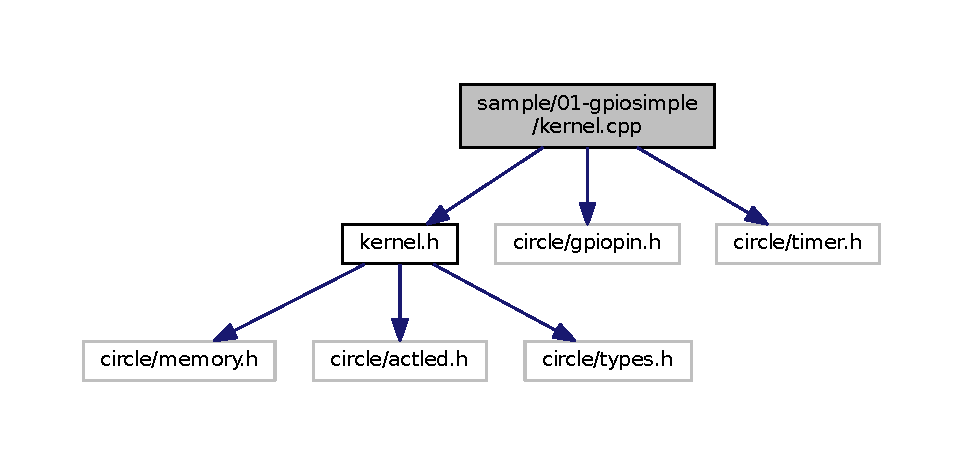
\includegraphics[width=350pt]{kernel_8cpp__incl}
\end{center}
\end{figure}

\hypertarget{kernel_8h}{}\section{sample/01-\/gpiosimple/kernel.h File Reference}
\label{kernel_8h}\index{sample/01-\/gpiosimple/kernel.\+h@{sample/01-\/gpiosimple/kernel.\+h}}
{\ttfamily \#include $<$circle/memory.\+h$>$}\\*
{\ttfamily \#include $<$circle/actled.\+h$>$}\\*
{\ttfamily \#include $<$circle/types.\+h$>$}\\*
Include dependency graph for kernel.\+h\+:
\nopagebreak
\begin{figure}[H]
\begin{center}
\leavevmode
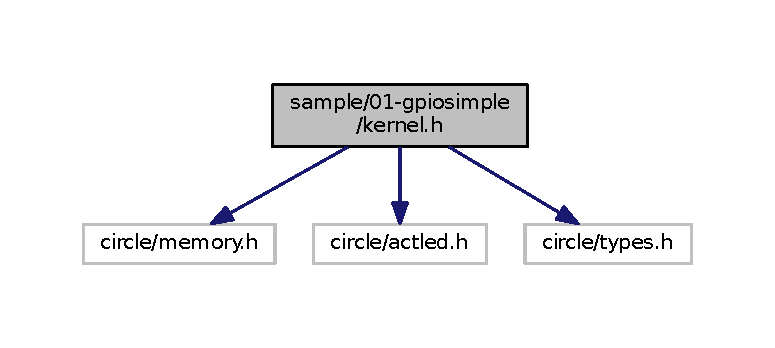
\includegraphics[width=350pt]{kernel_8h__incl}
\end{center}
\end{figure}
This graph shows which files directly or indirectly include this file\+:
\nopagebreak
\begin{figure}[H]
\begin{center}
\leavevmode
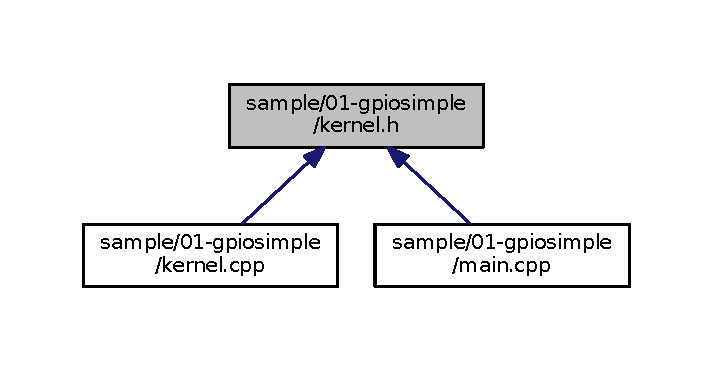
\includegraphics[width=342pt]{kernel_8h__dep__incl}
\end{center}
\end{figure}
\subsection*{Classes}
\begin{DoxyCompactItemize}
\item 
class \hyperlink{classCKernel}{C\+Kernel}
\end{DoxyCompactItemize}
\subsection*{Enumerations}
\begin{DoxyCompactItemize}
\item 
enum \hyperlink{kernel_8h_a1d97b873b27040859ad650950f96e569}{T\+Shutdown\+Mode} \{ \hyperlink{kernel_8h_a1d97b873b27040859ad650950f96e569acda4fe9e0029dbdde19f5aeeb39e32c3}{Shutdown\+None}, 
\hyperlink{kernel_8h_a1d97b873b27040859ad650950f96e569adb434133887b0ecaebccc475532549db}{Shutdown\+Halt}, 
\hyperlink{kernel_8h_a1d97b873b27040859ad650950f96e569a33fceebd4a59ddd4398a6075d9b4253c}{Shutdown\+Reboot}
 \}
\end{DoxyCompactItemize}


\subsection{Enumeration Type Documentation}
\index{kernel.\+h@{kernel.\+h}!T\+Shutdown\+Mode@{T\+Shutdown\+Mode}}
\index{T\+Shutdown\+Mode@{T\+Shutdown\+Mode}!kernel.\+h@{kernel.\+h}}
\subsubsection[{\texorpdfstring{T\+Shutdown\+Mode}{TShutdownMode}}]{\setlength{\rightskip}{0pt plus 5cm}enum {\bf T\+Shutdown\+Mode}}\hypertarget{kernel_8h_a1d97b873b27040859ad650950f96e569}{}\label{kernel_8h_a1d97b873b27040859ad650950f96e569}
\begin{Desc}
\item[Enumerator]\par
\begin{description}
\index{Shutdown\+None@{Shutdown\+None}!kernel.\+h@{kernel.\+h}}\index{kernel.\+h@{kernel.\+h}!Shutdown\+None@{Shutdown\+None}}\item[{\em 
Shutdown\+None\hypertarget{kernel_8h_a1d97b873b27040859ad650950f96e569acda4fe9e0029dbdde19f5aeeb39e32c3}{}\label{kernel_8h_a1d97b873b27040859ad650950f96e569acda4fe9e0029dbdde19f5aeeb39e32c3}
}]\index{Shutdown\+Halt@{Shutdown\+Halt}!kernel.\+h@{kernel.\+h}}\index{kernel.\+h@{kernel.\+h}!Shutdown\+Halt@{Shutdown\+Halt}}\item[{\em 
Shutdown\+Halt\hypertarget{kernel_8h_a1d97b873b27040859ad650950f96e569adb434133887b0ecaebccc475532549db}{}\label{kernel_8h_a1d97b873b27040859ad650950f96e569adb434133887b0ecaebccc475532549db}
}]\index{Shutdown\+Reboot@{Shutdown\+Reboot}!kernel.\+h@{kernel.\+h}}\index{kernel.\+h@{kernel.\+h}!Shutdown\+Reboot@{Shutdown\+Reboot}}\item[{\em 
Shutdown\+Reboot\hypertarget{kernel_8h_a1d97b873b27040859ad650950f96e569a33fceebd4a59ddd4398a6075d9b4253c}{}\label{kernel_8h_a1d97b873b27040859ad650950f96e569a33fceebd4a59ddd4398a6075d9b4253c}
}]\end{description}
\end{Desc}

\hypertarget{primeproc_8cpp}{}\section{src/apps/primeproc.cpp File Reference}
\label{primeproc_8cpp}\index{src/apps/primeproc.\+cpp@{src/apps/primeproc.\+cpp}}
{\ttfamily \#include \char`\"{}primeproc.\+h\char`\"{}}\\*
{\ttfamily \#include \char`\"{}circle/logger.\+h\char`\"{}}\\*
Include dependency graph for primeproc.\+cpp\+:
\nopagebreak
\begin{figure}[H]
\begin{center}
\leavevmode
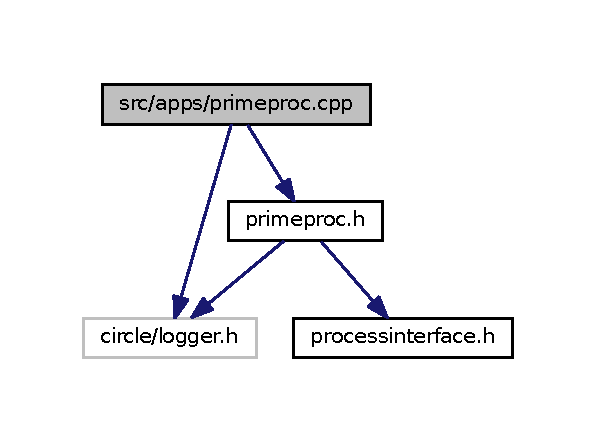
\includegraphics[width=286pt]{primeproc_8cpp__incl}
\end{center}
\end{figure}

\hypertarget{primeproc_8h}{}\section{src/apps/primeproc.h File Reference}
\label{primeproc_8h}\index{src/apps/primeproc.\+h@{src/apps/primeproc.\+h}}
{\ttfamily \#include $<$circle/logger.\+h$>$}\\*
{\ttfamily \#include $<$processinterface.\+h$>$}\\*
Include dependency graph for primeproc.\+h\+:
\nopagebreak
\begin{figure}[H]
\begin{center}
\leavevmode
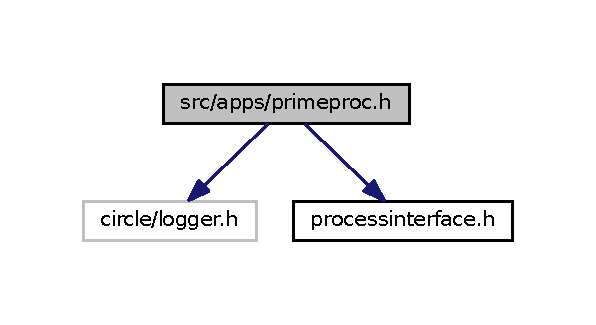
\includegraphics[width=286pt]{primeproc_8h__incl}
\end{center}
\end{figure}
This graph shows which files directly or indirectly include this file\+:
\nopagebreak
\begin{figure}[H]
\begin{center}
\leavevmode
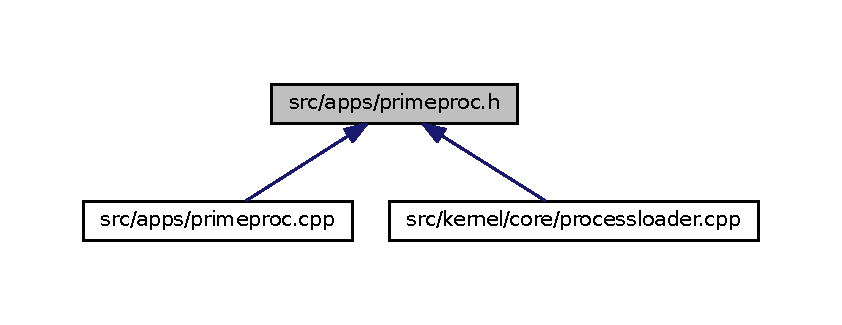
\includegraphics[width=350pt]{primeproc_8h__dep__incl}
\end{center}
\end{figure}
\subsection*{Classes}
\begin{DoxyCompactItemize}
\item 
class \hyperlink{classPrimeProc}{Prime\+Proc}
\end{DoxyCompactItemize}

\hypertarget{arch_8cpp}{}\section{src/kernel/arch/rasp4/arch.cpp File Reference}
\label{arch_8cpp}\index{src/kernel/arch/rasp4/arch.\+cpp@{src/kernel/arch/rasp4/arch.\+cpp}}
{\ttfamily \#include $<$arch.\+h$>$}\\*
{\ttfamily \#include $<$circle/debug.\+h$>$}\\*
{\ttfamily \#include $<$circle/gpiopin.\+h$>$}\\*
{\ttfamily \#include $<$circle/startup.\+h$>$}\\*
{\ttfamily \#include $<$circle/timer.\+h$>$}\\*
{\ttfamily \#include $<$errcode.\+h$>$}\\*
Include dependency graph for arch.\+cpp\+:
\nopagebreak
\begin{figure}[H]
\begin{center}
\leavevmode
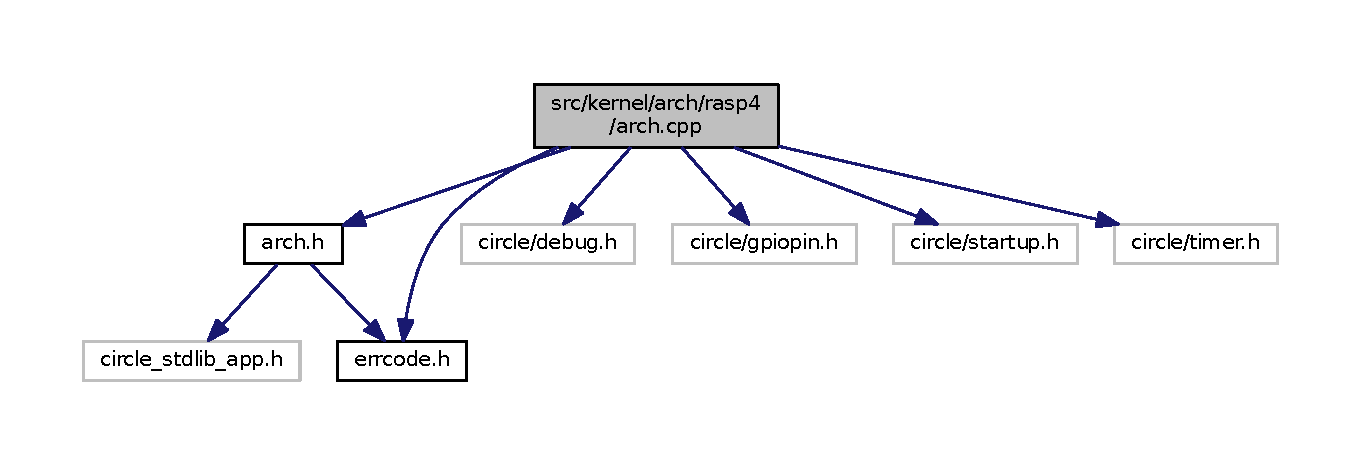
\includegraphics[width=350pt]{arch_8cpp__incl}
\end{center}
\end{figure}

\hypertarget{kernel_2arinc__module_8cpp}{}\section{src/kernel/arinc\+\_\+module.cpp File Reference}
\label{kernel_2arinc__module_8cpp}\index{src/kernel/arinc\+\_\+module.\+cpp@{src/kernel/arinc\+\_\+module.\+cpp}}
{\ttfamily \#include $<$arinc\+\_\+module.\+hpp$>$}\\*
Include dependency graph for arinc\+\_\+module.\+cpp\+:
\nopagebreak
\begin{figure}[H]
\begin{center}
\leavevmode
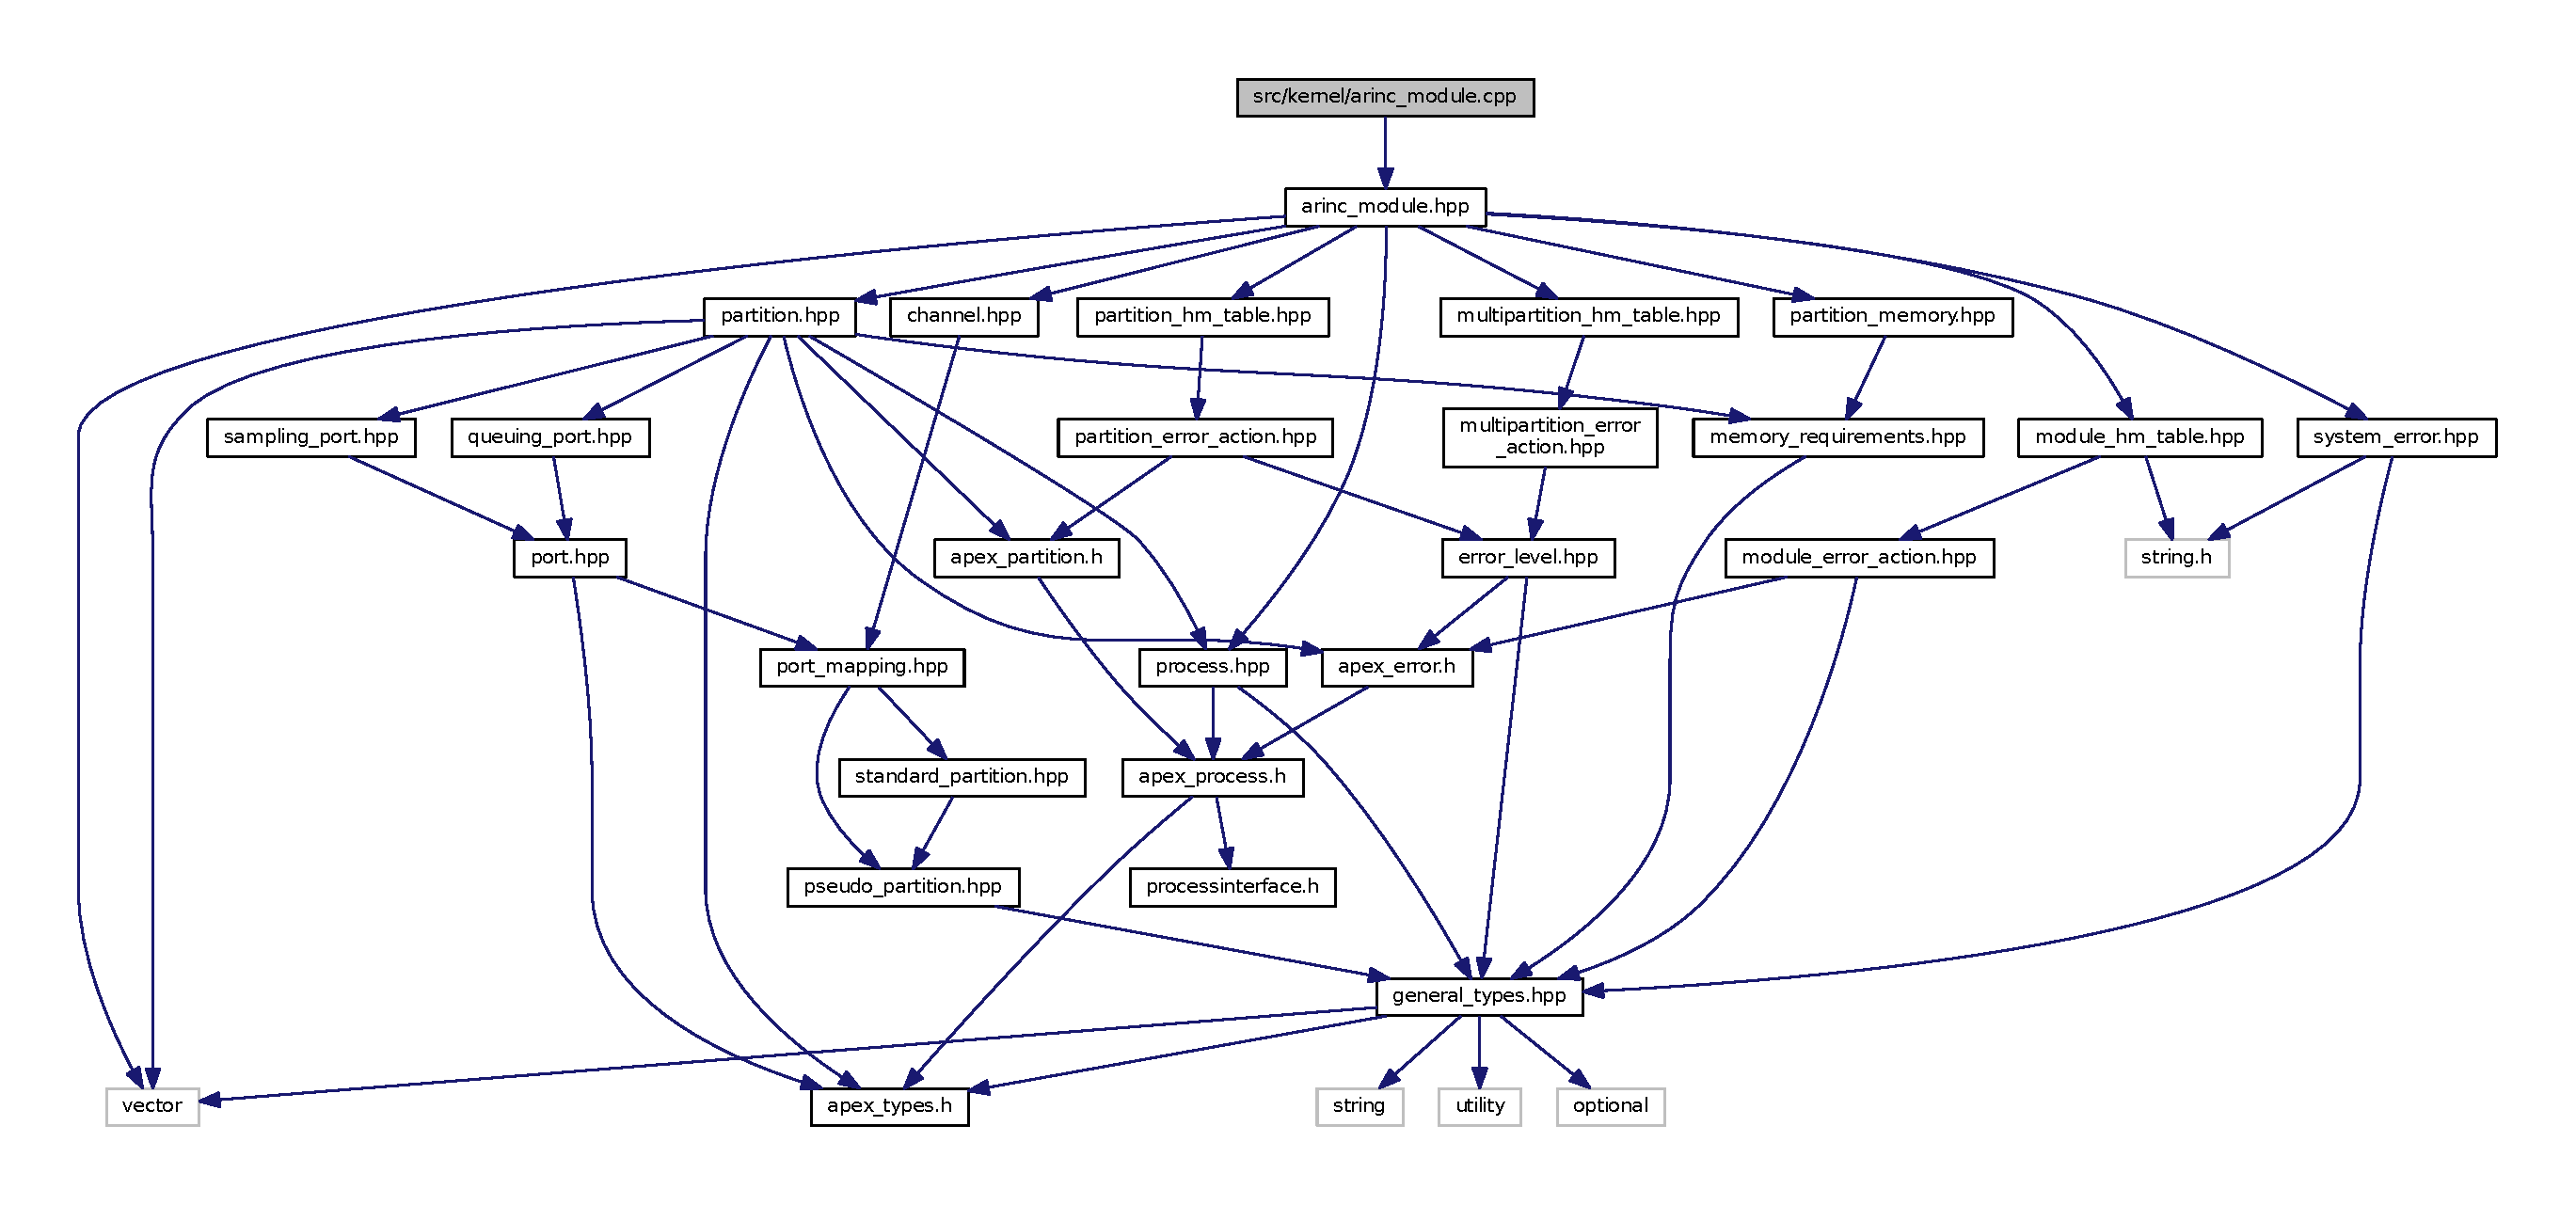
\includegraphics[width=350pt]{kernel_2arinc__module_8cpp__incl}
\end{center}
\end{figure}
\subsection*{Variables}
\begin{DoxyCompactItemize}
\item 
\hyperlink{classArincModule}{Arinc\+Module} \hyperlink{kernel_2arinc__module_8cpp_adba0da16a150788e2d976de247daa1d2}{arinc\+Module}
\end{DoxyCompactItemize}


\subsection{Variable Documentation}
\index{kernel/arinc\+\_\+module.\+cpp@{kernel/arinc\+\_\+module.\+cpp}!arinc\+Module@{arinc\+Module}}
\index{arinc\+Module@{arinc\+Module}!kernel/arinc\+\_\+module.\+cpp@{kernel/arinc\+\_\+module.\+cpp}}
\subsubsection[{\texorpdfstring{arinc\+Module}{arincModule}}]{\setlength{\rightskip}{0pt plus 5cm}{\bf Arinc\+Module} arinc\+Module}\hypertarget{kernel_2arinc__module_8cpp_adba0da16a150788e2d976de247daa1d2}{}\label{kernel_2arinc__module_8cpp_adba0da16a150788e2d976de247daa1d2}

\hypertarget{types_2src_2arinc__module_8cpp}{}\section{src/types/src/arinc\+\_\+module.cpp File Reference}
\label{types_2src_2arinc__module_8cpp}\index{src/types/src/arinc\+\_\+module.\+cpp@{src/types/src/arinc\+\_\+module.\+cpp}}
{\ttfamily \#include \char`\"{}include/arinc\+\_\+module.\+hpp\char`\"{}}\\*
Include dependency graph for arinc\+\_\+module.\+cpp\+:
\nopagebreak
\begin{figure}[H]
\begin{center}
\leavevmode
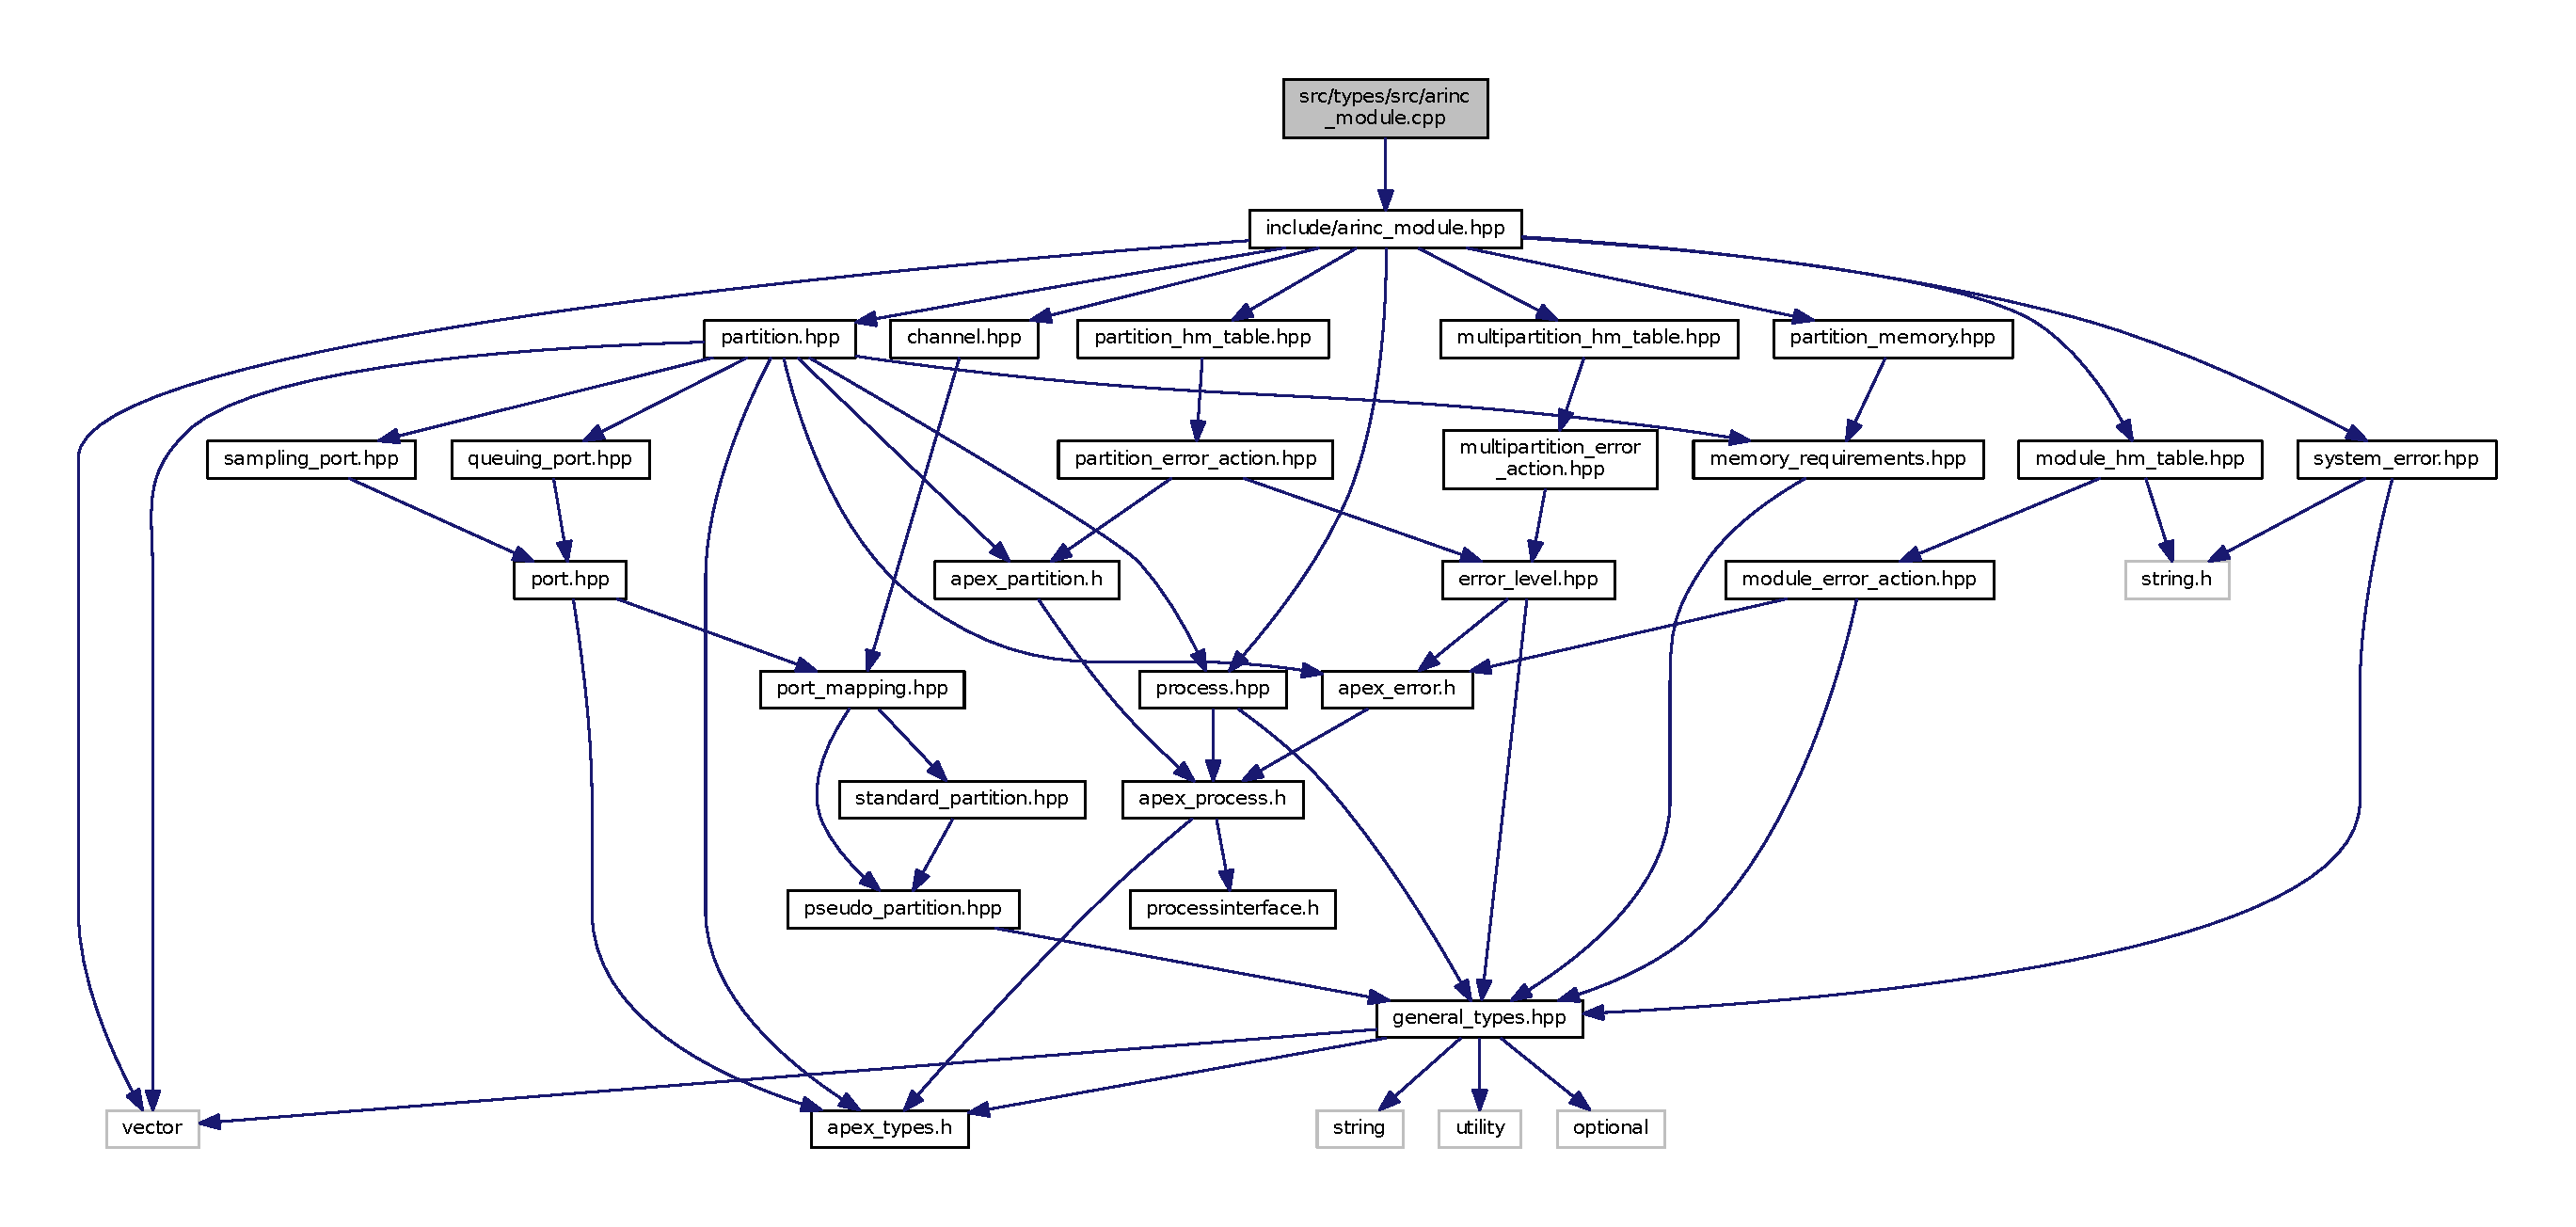
\includegraphics[width=350pt]{types_2src_2arinc__module_8cpp__incl}
\end{center}
\end{figure}

\hypertarget{config_8cpp}{}\section{src/kernel/config.cpp File Reference}
\label{config_8cpp}\index{src/kernel/config.\+cpp@{src/kernel/config.\+cpp}}
{\ttfamily \#include $<$arinc\+\_\+module.\+h$>$}\\*
{\ttfamily \#include $<$channel.\+h$>$}\\*
{\ttfamily \#include $<$error\+\_\+action.\+h$>$}\\*
{\ttfamily \#include $<$error\+\_\+level.\+h$>$}\\*
{\ttfamily \#include $<$general\+\_\+types.\+h$>$}\\*
{\ttfamily \#include $<$memory\+\_\+requirements.\+h$>$}\\*
{\ttfamily \#include $<$module\+\_\+hm\+\_\+table.\+h$>$}\\*
{\ttfamily \#include $<$multipartition\+\_\+hm\+\_\+table.\+h$>$}\\*
{\ttfamily \#include $<$partition.\+h$>$}\\*
{\ttfamily \#include $<$partition\+\_\+hm\+\_\+table.\+h$>$}\\*
{\ttfamily \#include $<$partition\+\_\+memory.\+h$>$}\\*
{\ttfamily \#include $<$port\+\_\+mapping.\+h$>$}\\*
{\ttfamily \#include $<$port\+\_\+type.\+h$>$}\\*
{\ttfamily \#include $<$process.\+h$>$}\\*
{\ttfamily \#include $<$pseudo\+\_\+standard\+\_\+partitions.\+h$>$}\\*
{\ttfamily \#include $<$schedule.\+h$>$}\\*
{\ttfamily \#include $<$system\+\_\+state\+\_\+entry.\+h$>$}\\*
{\ttfamily \#include $<$apex\+\_\+blackboard.\+h$>$}\\*
{\ttfamily \#include $<$apex\+\_\+queuing\+\_\+port.\+h$>$}\\*
{\ttfamily \#include $<$apex\+\_\+sampling\+\_\+port.\+h$>$}\\*
{\ttfamily \#include $<$apex\+\_\+buffer.\+h$>$}\\*
{\ttfamily \#include $<$apex\+\_\+error.\+h$>$}\\*
{\ttfamily \#include $<$apex\+\_\+event.\+h$>$}\\*
{\ttfamily \#include $<$apex\+\_\+partition.\+h$>$}\\*
{\ttfamily \#include $<$apex\+\_\+process.\+h$>$}\\*
{\ttfamily \#include $<$apex\+\_\+semaphore.\+h$>$}\\*
{\ttfamily \#include $<$apex\+\_\+time.\+h$>$}\\*
{\ttfamily \#include $<$apex\+\_\+types.\+h$>$}\\*
Include dependency graph for config.\+cpp\+:
\nopagebreak
\begin{figure}[H]
\begin{center}
\leavevmode
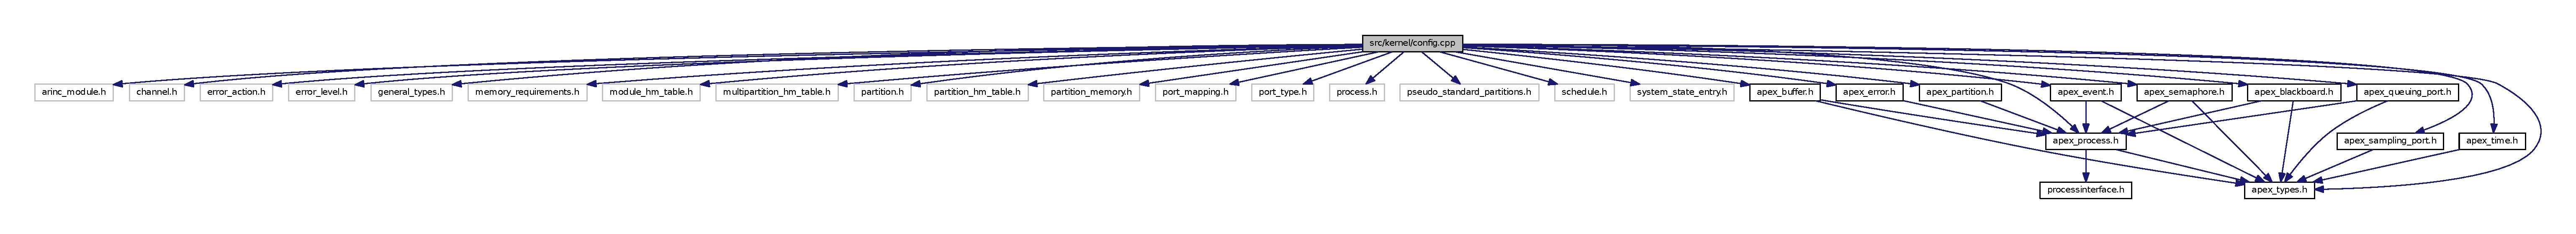
\includegraphics[width=350pt]{config_8cpp__incl}
\end{center}
\end{figure}
\subsection*{Variables}
\begin{DoxyCompactItemize}
\item 
\hyperlink{classArincModule}{Arinc\+Module} \hyperlink{config_8cpp_adba0da16a150788e2d976de247daa1d2}{arinc\+Module}
\end{DoxyCompactItemize}


\subsection{Variable Documentation}
\index{config.\+cpp@{config.\+cpp}!arinc\+Module@{arinc\+Module}}
\index{arinc\+Module@{arinc\+Module}!config.\+cpp@{config.\+cpp}}
\subsubsection[{\texorpdfstring{arinc\+Module}{arincModule}}]{\setlength{\rightskip}{0pt plus 5cm}{\bf Arinc\+Module} arinc\+Module}\hypertarget{config_8cpp_adba0da16a150788e2d976de247daa1d2}{}\label{config_8cpp_adba0da16a150788e2d976de247daa1d2}

\hypertarget{boot_8cpp}{}\section{src/kernel/core/boot.cpp File Reference}
\label{boot_8cpp}\index{src/kernel/core/boot.\+cpp@{src/kernel/core/boot.\+cpp}}
{\ttfamily \#include \char`\"{}tacoskernel.\+h\char`\"{}}\\*
{\ttfamily \#include $<$circle/startup.\+h$>$}\\*
{\ttfamily \#include $<$errcode.\+h$>$}\\*
Include dependency graph for boot.\+cpp\+:
\nopagebreak
\begin{figure}[H]
\begin{center}
\leavevmode
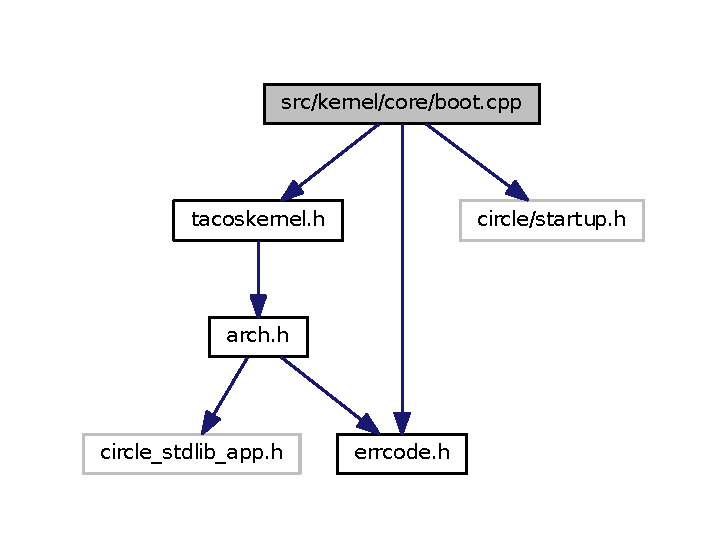
\includegraphics[width=349pt]{boot_8cpp__incl}
\end{center}
\end{figure}
\subsection*{Functions}
\begin{DoxyCompactItemize}
\item 
\hyperlink{errcode_8h_a18a6141fb52597a7d96dc02105928b47}{ret\+\_\+t} \hyperlink{boot_8cpp_a15b8741f917cb0a5c3506dd006ade09a}{boot} ()
\end{DoxyCompactItemize}


\subsection{Function Documentation}
\index{boot.\+cpp@{boot.\+cpp}!boot@{boot}}
\index{boot@{boot}!boot.\+cpp@{boot.\+cpp}}
\subsubsection[{\texorpdfstring{boot()}{boot()}}]{\setlength{\rightskip}{0pt plus 5cm}{\bf ret\+\_\+t} boot (
\begin{DoxyParamCaption}
{}
\end{DoxyParamCaption}
)}\hypertarget{boot_8cpp_a15b8741f917cb0a5c3506dd006ade09a}{}\label{boot_8cpp_a15b8741f917cb0a5c3506dd006ade09a}

\hypertarget{processinterface_8cpp}{}\section{src/kernel/core/process/processinterface.cpp File Reference}
\label{processinterface_8cpp}\index{src/kernel/core/process/processinterface.\+cpp@{src/kernel/core/process/processinterface.\+cpp}}

\hypertarget{processinterface_8h}{}\section{src/kernel/core/process/processinterface.h File Reference}
\label{processinterface_8h}\index{src/kernel/core/process/processinterface.\+h@{src/kernel/core/process/processinterface.\+h}}
This graph shows which files directly or indirectly include this file\+:
\nopagebreak
\begin{figure}[H]
\begin{center}
\leavevmode
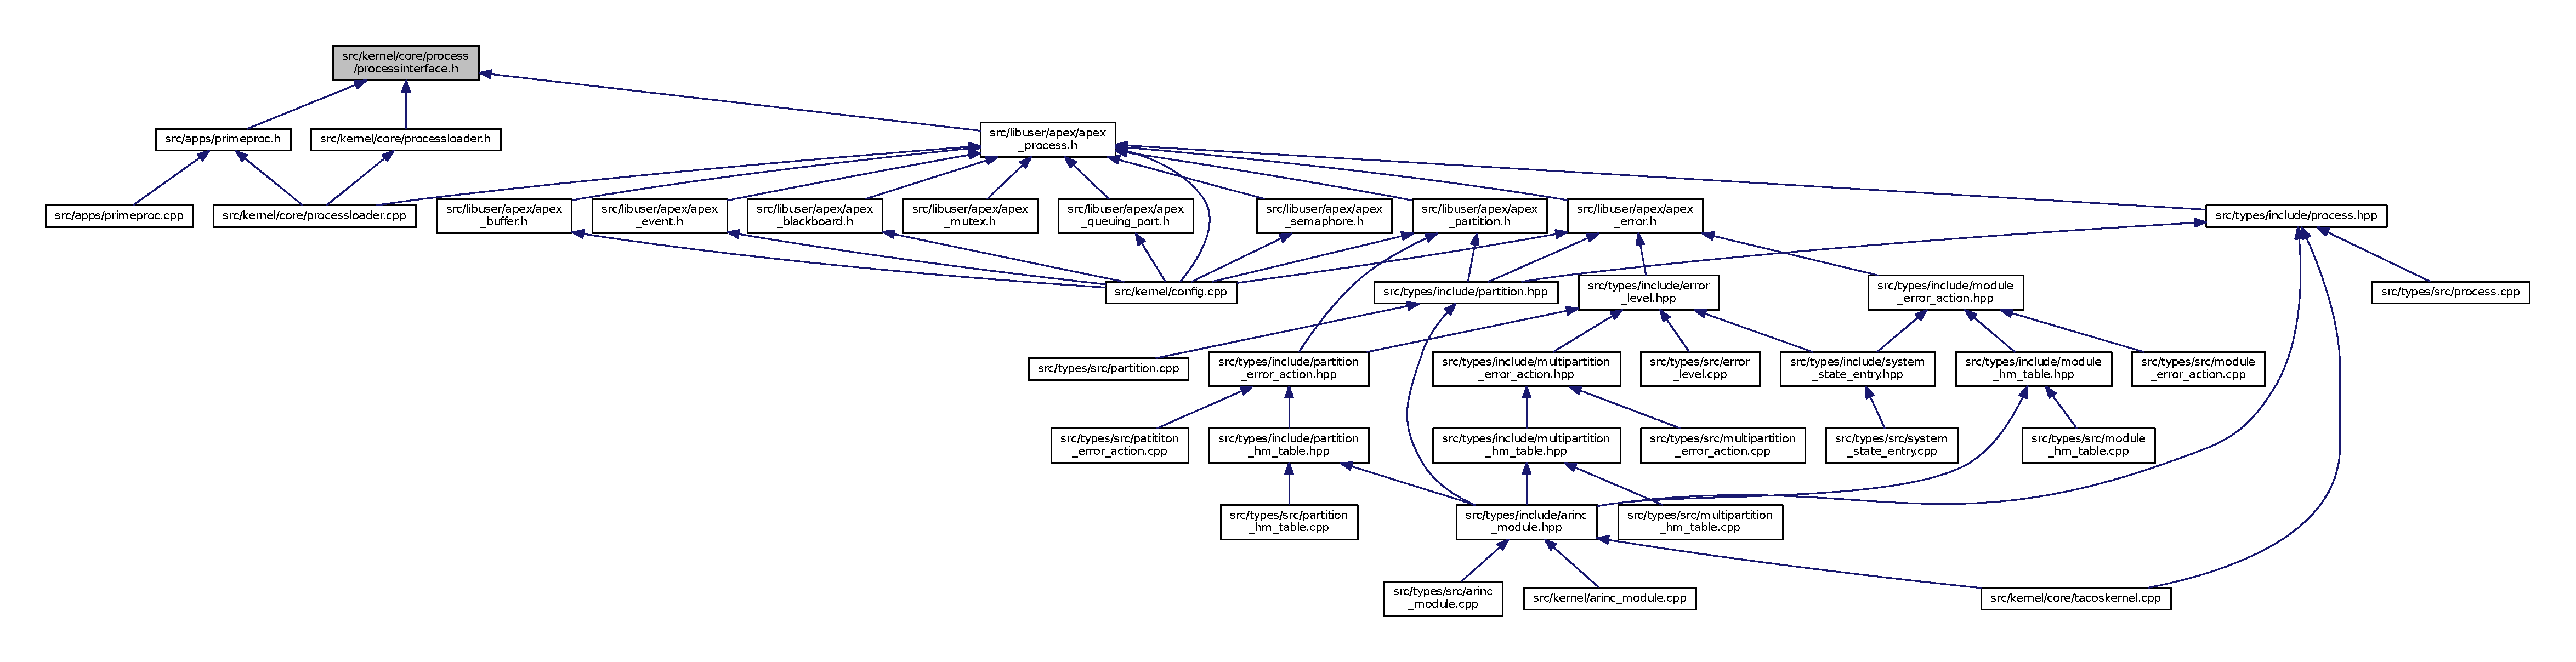
\includegraphics[width=350pt]{processinterface_8h__dep__incl}
\end{center}
\end{figure}
\subsection*{Classes}
\begin{DoxyCompactItemize}
\item 
class \hyperlink{classIProcess}{I\+Process}
\end{DoxyCompactItemize}

\hypertarget{processloader_8cpp}{}\section{src/kernel/core/processloader.cpp File Reference}
\label{processloader_8cpp}\index{src/kernel/core/processloader.\+cpp@{src/kernel/core/processloader.\+cpp}}
{\ttfamily \#include $<$apex\+\_\+process.\+h$>$}\\*
{\ttfamily \#include $<$primeproc.\+h$>$}\\*
{\ttfamily \#include $<$processloader.\+h$>$}\\*
Include dependency graph for processloader.\+cpp\+:
\nopagebreak
\begin{figure}[H]
\begin{center}
\leavevmode
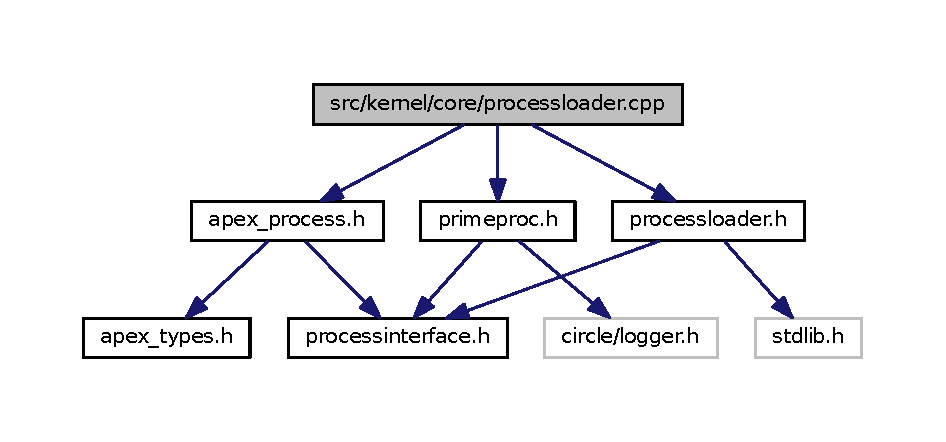
\includegraphics[width=350pt]{processloader_8cpp__incl}
\end{center}
\end{figure}
\subsection*{Typedefs}
\begin{DoxyCompactItemize}
\item 
typedef void \hyperlink{processloader_8cpp_a685ecbba18cc343f39fbb5336ba2aef6}{func}(void)
\end{DoxyCompactItemize}


\subsection{Typedef Documentation}
\index{processloader.\+cpp@{processloader.\+cpp}!func@{func}}
\index{func@{func}!processloader.\+cpp@{processloader.\+cpp}}
\subsubsection[{\texorpdfstring{func}{func}}]{\setlength{\rightskip}{0pt plus 5cm}typedef void func(void)}\hypertarget{processloader_8cpp_a685ecbba18cc343f39fbb5336ba2aef6}{}\label{processloader_8cpp_a685ecbba18cc343f39fbb5336ba2aef6}

\hypertarget{processloader_8h}{}\section{src/kernel/core/processloader.h File Reference}
\label{processloader_8h}\index{src/kernel/core/processloader.\+h@{src/kernel/core/processloader.\+h}}
{\ttfamily \#include $<$processinterface.\+h$>$}\\*
{\ttfamily \#include $<$stdlib.\+h$>$}\\*
Include dependency graph for processloader.\+h\+:
\nopagebreak
\begin{figure}[H]
\begin{center}
\leavevmode
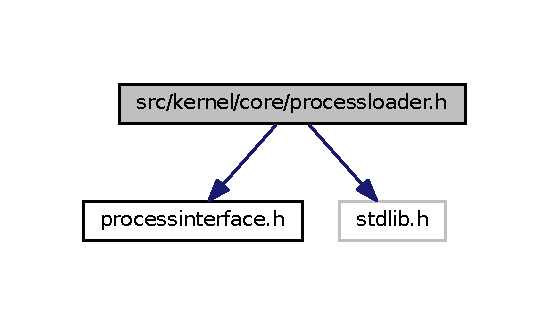
\includegraphics[width=264pt]{processloader_8h__incl}
\end{center}
\end{figure}
This graph shows which files directly or indirectly include this file\+:
\nopagebreak
\begin{figure}[H]
\begin{center}
\leavevmode
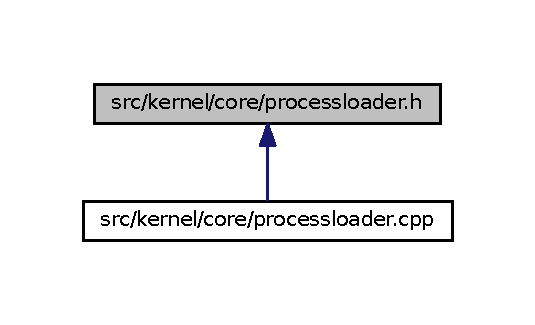
\includegraphics[width=257pt]{processloader_8h__dep__incl}
\end{center}
\end{figure}
\subsection*{Classes}
\begin{DoxyCompactItemize}
\item 
class \hyperlink{classProcessLoader}{Process\+Loader}
\end{DoxyCompactItemize}

\hypertarget{tacoskernel_8cpp}{}\section{src/kernel/core/tacoskernel.cpp File Reference}
\label{tacoskernel_8cpp}\index{src/kernel/core/tacoskernel.\+cpp@{src/kernel/core/tacoskernel.\+cpp}}
{\ttfamily \#include \char`\"{}tacoskernel.\+h\char`\"{}}\\*
{\ttfamily \#include $<$errcode.\+h$>$}\\*
{\ttfamily \#include $<$arinc\+\_\+module.\+hpp$>$}\\*
{\ttfamily \#include $<$process.\+hpp$>$}\\*
Include dependency graph for tacoskernel.\+cpp\+:
\nopagebreak
\begin{figure}[H]
\begin{center}
\leavevmode
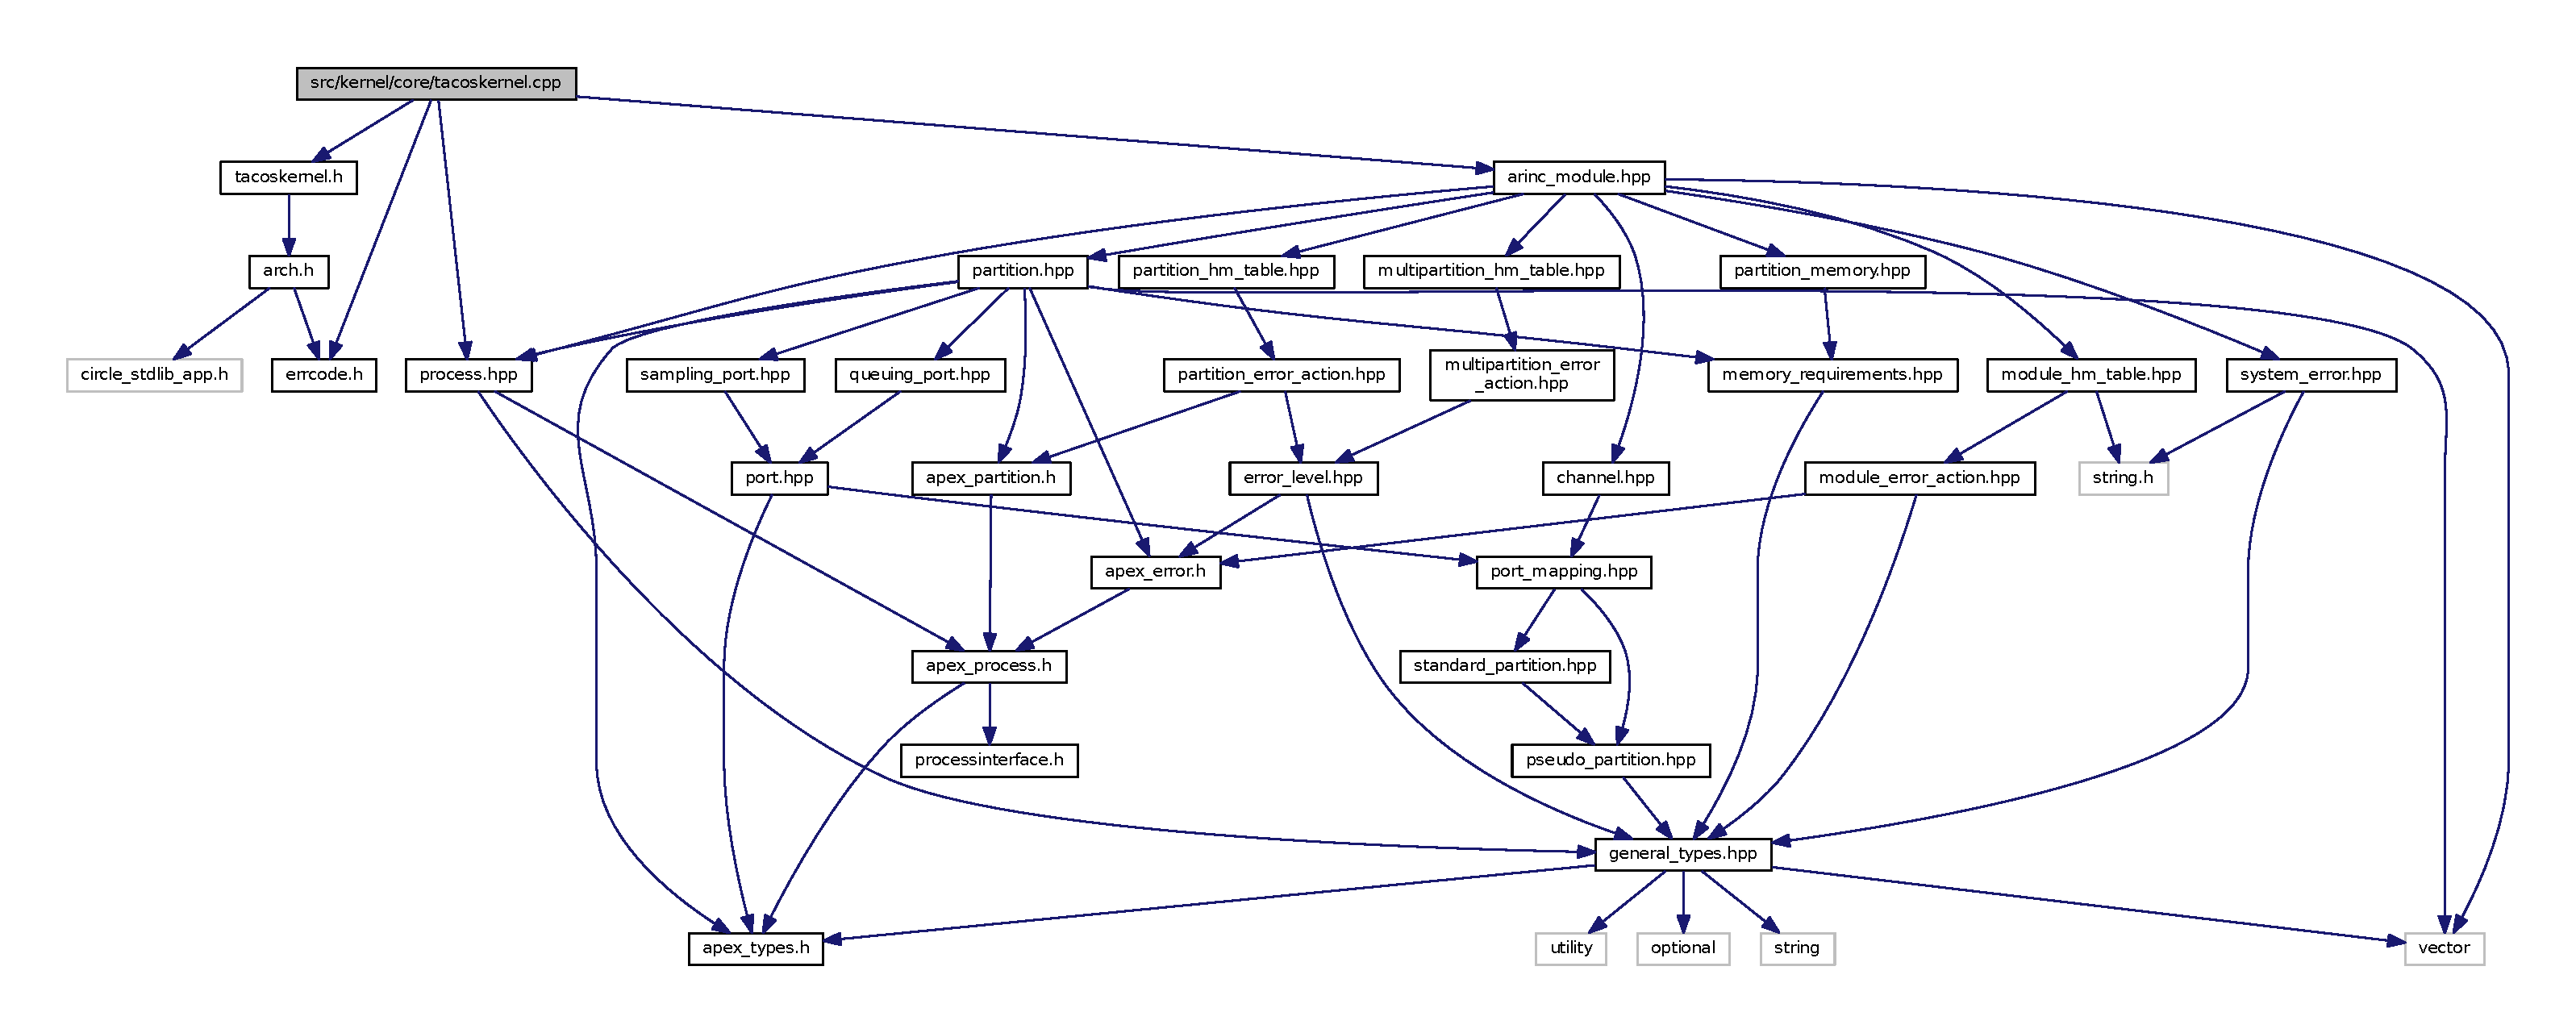
\includegraphics[width=350pt]{tacoskernel_8cpp__incl}
\end{center}
\end{figure}

\hypertarget{tacoskernel_8h}{}\section{src/kernel/core/tacoskernel.h File Reference}
\label{tacoskernel_8h}\index{src/kernel/core/tacoskernel.\+h@{src/kernel/core/tacoskernel.\+h}}
{\ttfamily \#include $<$arch.\+h$>$}\\*
Include dependency graph for tacoskernel.\+h\+:
\nopagebreak
\begin{figure}[H]
\begin{center}
\leavevmode
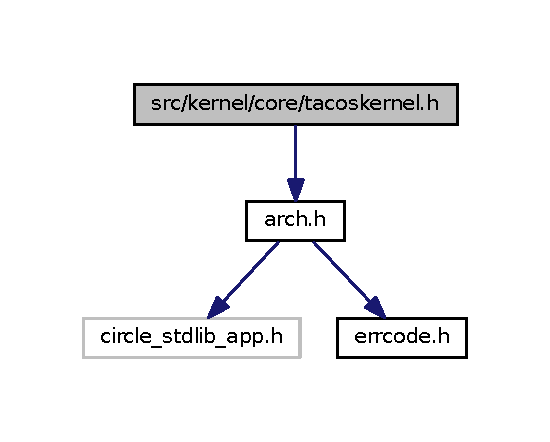
\includegraphics[width=264pt]{tacoskernel_8h__incl}
\end{center}
\end{figure}
This graph shows which files directly or indirectly include this file\+:
\nopagebreak
\begin{figure}[H]
\begin{center}
\leavevmode
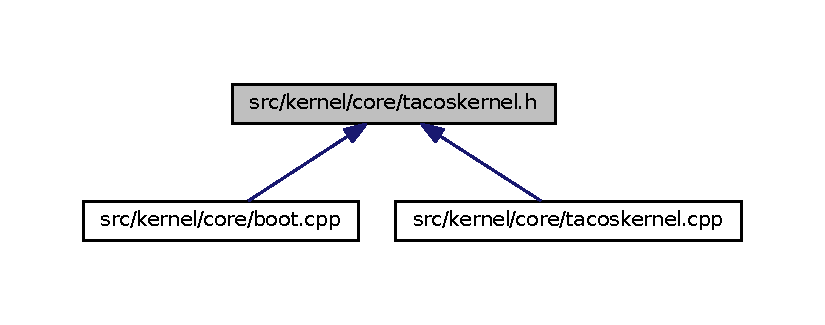
\includegraphics[width=350pt]{tacoskernel_8h__dep__incl}
\end{center}
\end{figure}
\subsection*{Classes}
\begin{DoxyCompactItemize}
\item 
class \hyperlink{classCTacosKernel}{C\+Tacos\+Kernel}
\end{DoxyCompactItemize}

\hypertarget{core__schedule_8cpp}{}\section{src/kernel/core\+\_\+schedule.cpp File Reference}
\label{core__schedule_8cpp}\index{src/kernel/core\+\_\+schedule.\+cpp@{src/kernel/core\+\_\+schedule.\+cpp}}
{\ttfamily \#include \char`\"{}core\+\_\+schedule.\+hpp\char`\"{}}\\*
Include dependency graph for core\+\_\+schedule.\+cpp\+:
\nopagebreak
\begin{figure}[H]
\begin{center}
\leavevmode
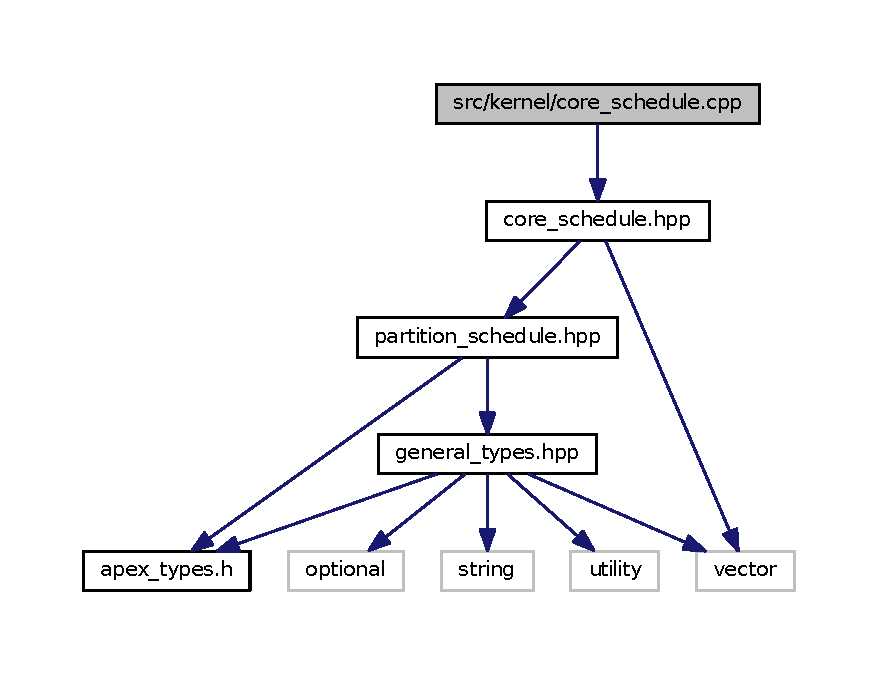
\includegraphics[width=350pt]{core__schedule_8cpp__incl}
\end{center}
\end{figure}
\subsection*{Variables}
\begin{DoxyCompactItemize}
\item 
\hyperlink{classCoreSchedule}{Core\+Schedule} \hyperlink{core__schedule_8cpp_a1e62c4b8fa9eccf7ca08b70ef60a0e87}{core\+Schedule}
\end{DoxyCompactItemize}


\subsection{Variable Documentation}
\index{core\+\_\+schedule.\+cpp@{core\+\_\+schedule.\+cpp}!core\+Schedule@{core\+Schedule}}
\index{core\+Schedule@{core\+Schedule}!core\+\_\+schedule.\+cpp@{core\+\_\+schedule.\+cpp}}
\subsubsection[{\texorpdfstring{core\+Schedule}{coreSchedule}}]{\setlength{\rightskip}{0pt plus 5cm}{\bf Core\+Schedule} core\+Schedule}\hypertarget{core__schedule_8cpp_a1e62c4b8fa9eccf7ca08b70ef60a0e87}{}\label{core__schedule_8cpp_a1e62c4b8fa9eccf7ca08b70ef60a0e87}

\hypertarget{arch_8h}{}\section{src/kernel/include/arch.h File Reference}
\label{arch_8h}\index{src/kernel/include/arch.\+h@{src/kernel/include/arch.\+h}}
{\ttfamily \#include $<$circle\+\_\+stdlib\+\_\+app.\+h$>$}\\*
{\ttfamily \#include $<$errcode.\+h$>$}\\*
Include dependency graph for arch.\+h\+:
\nopagebreak
\begin{figure}[H]
\begin{center}
\leavevmode
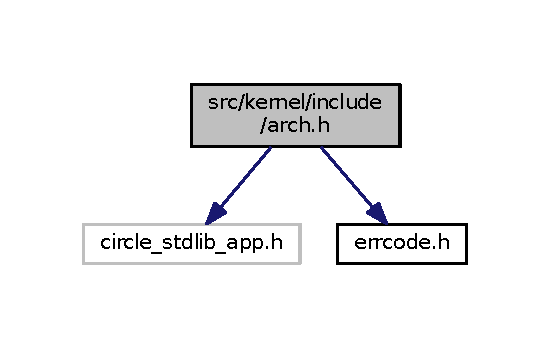
\includegraphics[width=264pt]{arch_8h__incl}
\end{center}
\end{figure}
This graph shows which files directly or indirectly include this file\+:
\nopagebreak
\begin{figure}[H]
\begin{center}
\leavevmode
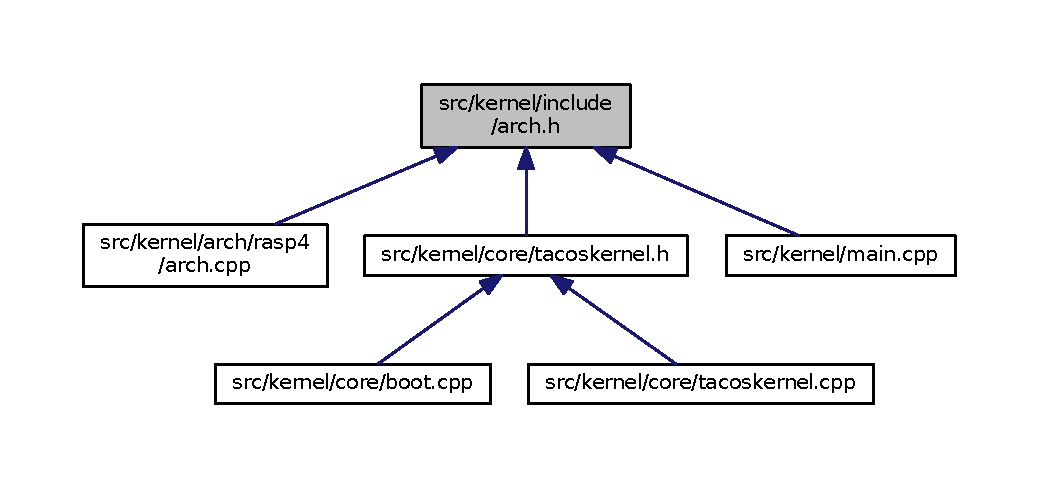
\includegraphics[width=350pt]{arch_8h__dep__incl}
\end{center}
\end{figure}
\subsection*{Classes}
\begin{DoxyCompactItemize}
\item 
class \hyperlink{classCKernel}{C\+Kernel}
\end{DoxyCompactItemize}

\hypertarget{boot_8h}{}\section{src/kernel/include/core/boot.h File Reference}
\label{boot_8h}\index{src/kernel/include/core/boot.\+h@{src/kernel/include/core/boot.\+h}}
{\ttfamily \#include $<$errcode.\+h$>$}\\*
Include dependency graph for boot.\+h\+:
\nopagebreak
\begin{figure}[H]
\begin{center}
\leavevmode
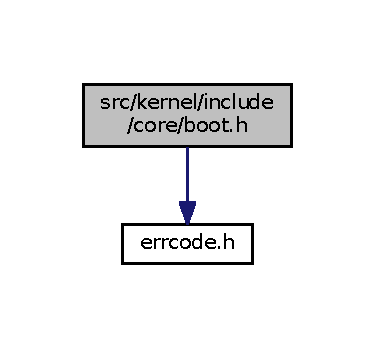
\includegraphics[width=180pt]{boot_8h__incl}
\end{center}
\end{figure}
This graph shows which files directly or indirectly include this file\+:\nopagebreak
\begin{figure}[H]
\begin{center}
\leavevmode
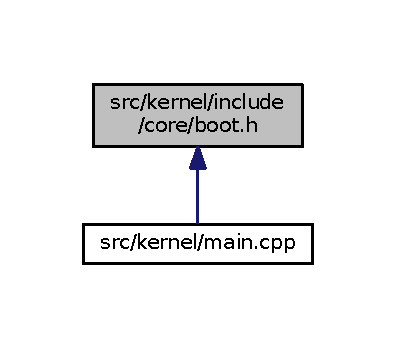
\includegraphics[width=190pt]{boot_8h__dep__incl}
\end{center}
\end{figure}
\subsection*{Functions}
\begin{DoxyCompactItemize}
\item 
void \hyperlink{boot_8h_a91f0d46e3cf4e047b0d97bf03252b40b}{free\+T\+A\+C\+O\+S\+\_\+boot} ()
\item 
\hyperlink{errcode_8h_a18a6141fb52597a7d96dc02105928b47}{ret\+\_\+t} \hyperlink{boot_8h_a15b8741f917cb0a5c3506dd006ade09a}{boot} ()
\end{DoxyCompactItemize}


\subsection{Function Documentation}
\index{boot.\+h@{boot.\+h}!boot@{boot}}
\index{boot@{boot}!boot.\+h@{boot.\+h}}
\subsubsection[{\texorpdfstring{boot()}{boot()}}]{\setlength{\rightskip}{0pt plus 5cm}{\bf ret\+\_\+t} boot (
\begin{DoxyParamCaption}
{}
\end{DoxyParamCaption}
)}\hypertarget{boot_8h_a15b8741f917cb0a5c3506dd006ade09a}{}\label{boot_8h_a15b8741f917cb0a5c3506dd006ade09a}
\index{boot.\+h@{boot.\+h}!free\+T\+A\+C\+O\+S\+\_\+boot@{free\+T\+A\+C\+O\+S\+\_\+boot}}
\index{free\+T\+A\+C\+O\+S\+\_\+boot@{free\+T\+A\+C\+O\+S\+\_\+boot}!boot.\+h@{boot.\+h}}
\subsubsection[{\texorpdfstring{free\+T\+A\+C\+O\+S\+\_\+boot()}{freeTACOS_boot()}}]{\setlength{\rightskip}{0pt plus 5cm}void free\+T\+A\+C\+O\+S\+\_\+boot (
\begin{DoxyParamCaption}
{}
\end{DoxyParamCaption}
)}\hypertarget{boot_8h_a91f0d46e3cf4e047b0d97bf03252b40b}{}\label{boot_8h_a91f0d46e3cf4e047b0d97bf03252b40b}

\hypertarget{errcode_8h}{}\section{src/kernel/include/errcode.h File Reference}
\label{errcode_8h}\index{src/kernel/include/errcode.\+h@{src/kernel/include/errcode.\+h}}
This graph shows which files directly or indirectly include this file\+:
\nopagebreak
\begin{figure}[H]
\begin{center}
\leavevmode
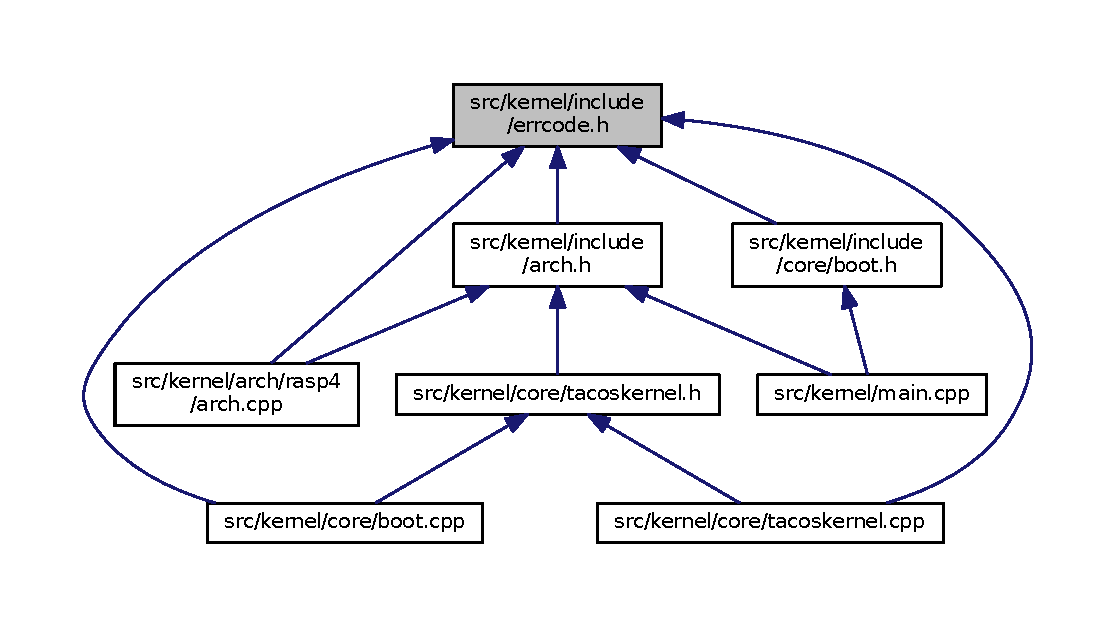
\includegraphics[width=350pt]{errcode_8h__dep__incl}
\end{center}
\end{figure}
\subsection*{Enumerations}
\begin{DoxyCompactItemize}
\item 
enum \hyperlink{errcode_8h_a18a6141fb52597a7d96dc02105928b47}{ret\+\_\+t} \{ \hyperlink{errcode_8h_a18a6141fb52597a7d96dc02105928b47ad8b76af209cd7ba83b4ebf33ba1637b2}{ok} = 0
 \}
\end{DoxyCompactItemize}


\subsection{Enumeration Type Documentation}
\index{errcode.\+h@{errcode.\+h}!ret\+\_\+t@{ret\+\_\+t}}
\index{ret\+\_\+t@{ret\+\_\+t}!errcode.\+h@{errcode.\+h}}
\subsubsection[{\texorpdfstring{ret\+\_\+t}{ret_t}}]{\setlength{\rightskip}{0pt plus 5cm}enum {\bf ret\+\_\+t}}\hypertarget{errcode_8h_a18a6141fb52597a7d96dc02105928b47}{}\label{errcode_8h_a18a6141fb52597a7d96dc02105928b47}
\begin{Desc}
\item[Enumerator]\par
\begin{description}
\index{ok@{ok}!errcode.\+h@{errcode.\+h}}\index{errcode.\+h@{errcode.\+h}!ok@{ok}}\item[{\em 
ok\hypertarget{errcode_8h_a18a6141fb52597a7d96dc02105928b47ad8b76af209cd7ba83b4ebf33ba1637b2}{}\label{errcode_8h_a18a6141fb52597a7d96dc02105928b47ad8b76af209cd7ba83b4ebf33ba1637b2}
}]\end{description}
\end{Desc}

\hypertarget{src_2kernel_2main_8cpp}{}\section{src/kernel/main.cpp File Reference}
\label{src_2kernel_2main_8cpp}\index{src/kernel/main.\+cpp@{src/kernel/main.\+cpp}}
{\ttfamily \#include $<$arch.\+h$>$}\\*
{\ttfamily \#include $<$core/boot.\+h$>$}\\*
Include dependency graph for main.\+cpp\+:
\nopagebreak
\begin{figure}[H]
\begin{center}
\leavevmode
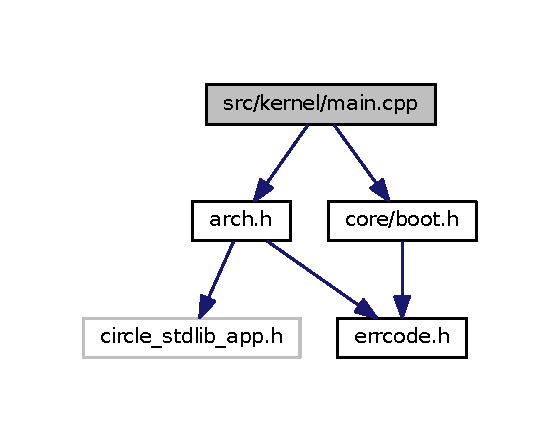
\includegraphics[width=269pt]{src_2kernel_2main_8cpp__incl}
\end{center}
\end{figure}
\subsection*{Functions}
\begin{DoxyCompactItemize}
\item 
int \hyperlink{src_2kernel_2main_8cpp_a840291bc02cba5474a4cb46a9b9566fe}{main} (void)
\end{DoxyCompactItemize}


\subsection{Function Documentation}
\index{src/kernel/main.\+cpp@{src/kernel/main.\+cpp}!main@{main}}
\index{main@{main}!src/kernel/main.\+cpp@{src/kernel/main.\+cpp}}
\subsubsection[{\texorpdfstring{main(void)}{main(void)}}]{\setlength{\rightskip}{0pt plus 5cm}int main (
\begin{DoxyParamCaption}
\item[{void}]{}
\end{DoxyParamCaption}
)}\hypertarget{src_2kernel_2main_8cpp_a840291bc02cba5474a4cb46a9b9566fe}{}\label{src_2kernel_2main_8cpp_a840291bc02cba5474a4cb46a9b9566fe}

\hypertarget{src_2main_8cpp}{}\section{src/main.cpp File Reference}
\label{src_2main_8cpp}\index{src/main.\+cpp@{src/main.\+cpp}}
{\ttfamily \#include \char`\"{}types/arinc\+\_\+module.\+h\char`\"{}}\\*
Include dependency graph for main.\+cpp\+:
\nopagebreak
\begin{figure}[H]
\begin{center}
\leavevmode
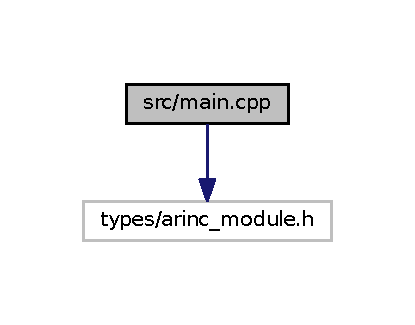
\includegraphics[width=199pt]{src_2main_8cpp__incl}
\end{center}
\end{figure}
\subsection*{Functions}
\begin{DoxyCompactItemize}
\item 
int \hyperlink{src_2main_8cpp_ae66f6b31b5ad750f1fe042a706a4e3d4}{main} ()
\end{DoxyCompactItemize}


\subsection{Function Documentation}
\index{src/main.\+cpp@{src/main.\+cpp}!main@{main}}
\index{main@{main}!src/main.\+cpp@{src/main.\+cpp}}
\subsubsection[{\texorpdfstring{main()}{main()}}]{\setlength{\rightskip}{0pt plus 5cm}int main (
\begin{DoxyParamCaption}
\item[{void}]{}
\end{DoxyParamCaption}
)}\hypertarget{src_2main_8cpp_ae66f6b31b5ad750f1fe042a706a4e3d4}{}\label{src_2main_8cpp_ae66f6b31b5ad750f1fe042a706a4e3d4}

\hypertarget{sample_201-gpiosimple_2main_8cpp}{}\section{sample/01-\/gpiosimple/main.cpp File Reference}
\label{sample_201-gpiosimple_2main_8cpp}\index{sample/01-\/gpiosimple/main.\+cpp@{sample/01-\/gpiosimple/main.\+cpp}}
{\ttfamily \#include \char`\"{}kernel.\+h\char`\"{}}\\*
{\ttfamily \#include $<$circle/startup.\+h$>$}\\*
Include dependency graph for main.\+cpp\+:\nopagebreak
\begin{figure}[H]
\begin{center}
\leavevmode
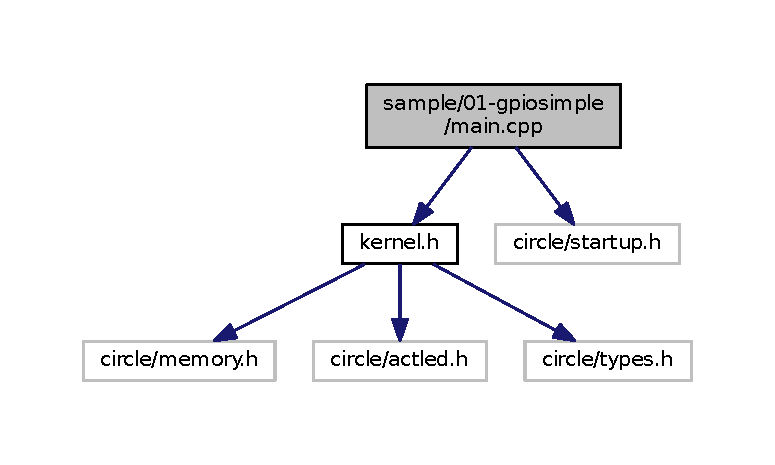
\includegraphics[width=350pt]{sample_201-gpiosimple_2main_8cpp__incl}
\end{center}
\end{figure}
\subsection*{Functions}
\begin{DoxyCompactItemize}
\item 
int \hyperlink{sample_201-gpiosimple_2main_8cpp_a840291bc02cba5474a4cb46a9b9566fe}{main} (void)
\end{DoxyCompactItemize}


\subsection{Function Documentation}
\index{sample/01-\/gpiosimple/main.\+cpp@{sample/01-\/gpiosimple/main.\+cpp}!main@{main}}
\index{main@{main}!sample/01-\/gpiosimple/main.\+cpp@{sample/01-\/gpiosimple/main.\+cpp}}
\subsubsection[{\texorpdfstring{main(void)}{main(void)}}]{\setlength{\rightskip}{0pt plus 5cm}int main (
\begin{DoxyParamCaption}
\item[{void}]{}
\end{DoxyParamCaption}
)}\hypertarget{sample_201-gpiosimple_2main_8cpp_a840291bc02cba5474a4cb46a9b9566fe}{}\label{sample_201-gpiosimple_2main_8cpp_a840291bc02cba5474a4cb46a9b9566fe}

\hypertarget{apex__blackboard_8h}{}\section{src/libuser/apex/apex\+\_\+blackboard.h File Reference}
\label{apex__blackboard_8h}\index{src/libuser/apex/apex\+\_\+blackboard.\+h@{src/libuser/apex/apex\+\_\+blackboard.\+h}}
{\ttfamily \#include \char`\"{}apex\+\_\+types.\+h\char`\"{}}\\*
{\ttfamily \#include \char`\"{}apex\+\_\+process.\+h\char`\"{}}\\*
Include dependency graph for apex\+\_\+blackboard.\+h\+:
\nopagebreak
\begin{figure}[H]
\begin{center}
\leavevmode
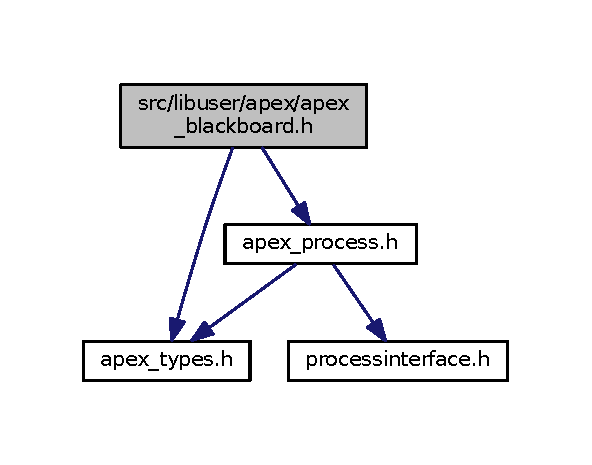
\includegraphics[width=284pt]{apex__blackboard_8h__incl}
\end{center}
\end{figure}
This graph shows which files directly or indirectly include this file\+:
\nopagebreak
\begin{figure}[H]
\begin{center}
\leavevmode
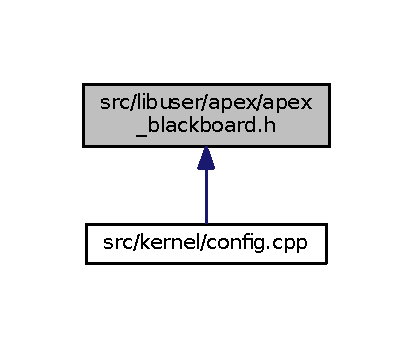
\includegraphics[width=198pt]{apex__blackboard_8h__dep__incl}
\end{center}
\end{figure}
\subsection*{Classes}
\begin{DoxyCompactItemize}
\item 
struct \hyperlink{structBLACKBOARD__STATUS__TYPE}{B\+L\+A\+C\+K\+B\+O\+A\+R\+D\+\_\+\+S\+T\+A\+T\+U\+S\+\_\+\+T\+Y\+PE}
\end{DoxyCompactItemize}
\subsection*{Macros}
\begin{DoxyCompactItemize}
\item 
\#define \hyperlink{apex__blackboard_8h_a5ba02936a02254292c27e7e9291dc8ff}{M\+A\+X\+\_\+\+N\+U\+M\+B\+E\+R\+\_\+\+O\+F\+\_\+\+B\+L\+A\+C\+K\+B\+O\+A\+R\+DS}~\hyperlink{apex__types_8h_ae9b83e2642f51335ec7e47f1f2490395}{S\+Y\+S\+T\+E\+M\+\_\+\+L\+I\+M\+I\+T\+\_\+\+N\+U\+M\+B\+E\+R\+\_\+\+O\+F\+\_\+\+B\+L\+A\+C\+K\+B\+O\+A\+R\+DS}
\end{DoxyCompactItemize}
\subsection*{Typedefs}
\begin{DoxyCompactItemize}
\item 
typedef \hyperlink{structNAME__TYPE}{N\+A\+M\+E\+\_\+\+T\+Y\+PE} \hyperlink{apex__blackboard_8h_a06c38eb2f1617704d63362ec889f6a3f}{B\+L\+A\+C\+K\+B\+O\+A\+R\+D\+\_\+\+N\+A\+M\+E\+\_\+\+T\+Y\+PE}
\item 
typedef \hyperlink{apex__types_8h_a4e13487a80a5740717e19f7f693e06c3}{A\+P\+E\+X\+\_\+\+I\+N\+T\+E\+G\+ER} \hyperlink{apex__blackboard_8h_aacc3e66182132c413b5be3eb604c25e4}{B\+L\+A\+C\+K\+B\+O\+A\+R\+D\+\_\+\+I\+D\+\_\+\+T\+Y\+PE}
\end{DoxyCompactItemize}
\subsection*{Enumerations}
\begin{DoxyCompactItemize}
\item 
enum \hyperlink{apex__blackboard_8h_a52d437b2fe6a3f155749fdb1728945dc}{E\+M\+P\+T\+Y\+\_\+\+I\+N\+D\+I\+C\+A\+T\+O\+R\+\_\+\+T\+Y\+PE} \{ \hyperlink{apex__blackboard_8h_a52d437b2fe6a3f155749fdb1728945dca2f0d18fc0d0fa4a6cd92dc328501874d}{E\+M\+P\+TY} = 0, 
\hyperlink{apex__blackboard_8h_a52d437b2fe6a3f155749fdb1728945dcaee22b30981d95b98502855b168330dc3}{O\+C\+C\+U\+P\+I\+ED} = 1
 \}
\end{DoxyCompactItemize}
\subsection*{Functions}
\begin{DoxyCompactItemize}
\item 
void \hyperlink{apex__blackboard_8h_a0fe217cf6b2c45a0f21bab65999c498b}{C\+R\+E\+A\+T\+E\+\_\+\+B\+L\+A\+C\+K\+B\+O\+A\+RD} (\hyperlink{apex__blackboard_8h_a06c38eb2f1617704d63362ec889f6a3f}{B\+L\+A\+C\+K\+B\+O\+A\+R\+D\+\_\+\+N\+A\+M\+E\+\_\+\+T\+Y\+PE} B\+L\+A\+C\+K\+B\+O\+A\+R\+D\+\_\+\+N\+A\+ME, \hyperlink{apex__types_8h_ae09494a8d78c38c94f0cc5a80e69785a}{M\+E\+S\+S\+A\+G\+E\+\_\+\+S\+I\+Z\+E\+\_\+\+T\+Y\+PE} M\+A\+X\+\_\+\+M\+E\+S\+S\+A\+G\+E\+\_\+\+S\+I\+ZE, \hyperlink{apex__blackboard_8h_aacc3e66182132c413b5be3eb604c25e4}{B\+L\+A\+C\+K\+B\+O\+A\+R\+D\+\_\+\+I\+D\+\_\+\+T\+Y\+PE} $\ast$B\+L\+A\+C\+K\+B\+O\+A\+R\+D\+\_\+\+ID, \hyperlink{apex__types_8h_a5cd52791e89e2513bef42ff9193691aa}{R\+E\+T\+U\+R\+N\+\_\+\+C\+O\+D\+E\+\_\+\+T\+Y\+PE} $\ast$R\+E\+T\+U\+R\+N\+\_\+\+C\+O\+DE)
\item 
void \hyperlink{apex__blackboard_8h_a57f00b25c8f793a3601c0d81f4c8571c}{D\+I\+S\+P\+L\+A\+Y\+\_\+\+B\+L\+A\+C\+K\+B\+O\+A\+RD} (\hyperlink{apex__blackboard_8h_aacc3e66182132c413b5be3eb604c25e4}{B\+L\+A\+C\+K\+B\+O\+A\+R\+D\+\_\+\+I\+D\+\_\+\+T\+Y\+PE} B\+L\+A\+C\+K\+B\+O\+A\+R\+D\+\_\+\+ID, \hyperlink{apex__types_8h_a1c9c3acbb8c99c2cbc7751db5226b1fc}{M\+E\+S\+S\+A\+G\+E\+\_\+\+A\+D\+D\+R\+\_\+\+T\+Y\+PE} M\+E\+S\+S\+A\+G\+E\+\_\+\+A\+D\+DR, \hyperlink{apex__types_8h_ae09494a8d78c38c94f0cc5a80e69785a}{M\+E\+S\+S\+A\+G\+E\+\_\+\+S\+I\+Z\+E\+\_\+\+T\+Y\+PE} L\+E\+N\+G\+TH, \hyperlink{apex__types_8h_a5cd52791e89e2513bef42ff9193691aa}{R\+E\+T\+U\+R\+N\+\_\+\+C\+O\+D\+E\+\_\+\+T\+Y\+PE} $\ast$R\+E\+T\+U\+R\+N\+\_\+\+C\+O\+DE)
\item 
void \hyperlink{apex__blackboard_8h_a63d9ad659c49d74853bb3b0e55d05f28}{R\+E\+A\+D\+\_\+\+B\+L\+A\+C\+K\+B\+O\+A\+RD} (\hyperlink{apex__blackboard_8h_aacc3e66182132c413b5be3eb604c25e4}{B\+L\+A\+C\+K\+B\+O\+A\+R\+D\+\_\+\+I\+D\+\_\+\+T\+Y\+PE} B\+L\+A\+C\+K\+B\+O\+A\+R\+D\+\_\+\+ID, \hyperlink{apex__types_8h_a78cd52c2621ddf2eda68fcd4bedbc1a7}{S\+Y\+S\+T\+E\+M\+\_\+\+T\+I\+M\+E\+\_\+\+T\+Y\+PE} T\+I\+M\+E\+\_\+\+O\+UT, \hyperlink{apex__types_8h_a1c9c3acbb8c99c2cbc7751db5226b1fc}{M\+E\+S\+S\+A\+G\+E\+\_\+\+A\+D\+D\+R\+\_\+\+T\+Y\+PE} M\+E\+S\+S\+A\+G\+E\+\_\+\+A\+D\+DR, \hyperlink{apex__types_8h_ae09494a8d78c38c94f0cc5a80e69785a}{M\+E\+S\+S\+A\+G\+E\+\_\+\+S\+I\+Z\+E\+\_\+\+T\+Y\+PE} $\ast$L\+E\+N\+G\+TH, \hyperlink{apex__types_8h_a5cd52791e89e2513bef42ff9193691aa}{R\+E\+T\+U\+R\+N\+\_\+\+C\+O\+D\+E\+\_\+\+T\+Y\+PE} $\ast$R\+E\+T\+U\+R\+N\+\_\+\+C\+O\+DE)
\item 
void \hyperlink{apex__blackboard_8h_a19da503fd9babf67bf16e6da247c5a0b}{C\+L\+E\+A\+R\+\_\+\+B\+L\+A\+C\+K\+B\+O\+A\+RD} (\hyperlink{apex__blackboard_8h_aacc3e66182132c413b5be3eb604c25e4}{B\+L\+A\+C\+K\+B\+O\+A\+R\+D\+\_\+\+I\+D\+\_\+\+T\+Y\+PE} B\+L\+A\+C\+K\+B\+O\+A\+R\+D\+\_\+\+ID, \hyperlink{apex__types_8h_a5cd52791e89e2513bef42ff9193691aa}{R\+E\+T\+U\+R\+N\+\_\+\+C\+O\+D\+E\+\_\+\+T\+Y\+PE} $\ast$R\+E\+T\+U\+R\+N\+\_\+\+C\+O\+DE)
\item 
void \hyperlink{apex__blackboard_8h_a3432bed49bdb1b6019c4fd4faae47028}{G\+E\+T\+\_\+\+B\+L\+A\+C\+K\+B\+O\+A\+R\+D\+\_\+\+ID} (\hyperlink{apex__blackboard_8h_a06c38eb2f1617704d63362ec889f6a3f}{B\+L\+A\+C\+K\+B\+O\+A\+R\+D\+\_\+\+N\+A\+M\+E\+\_\+\+T\+Y\+PE} B\+L\+A\+C\+K\+B\+O\+A\+R\+D\+\_\+\+N\+A\+ME, \hyperlink{apex__blackboard_8h_aacc3e66182132c413b5be3eb604c25e4}{B\+L\+A\+C\+K\+B\+O\+A\+R\+D\+\_\+\+I\+D\+\_\+\+T\+Y\+PE} $\ast$B\+L\+A\+C\+K\+B\+O\+A\+R\+D\+\_\+\+ID, \hyperlink{apex__types_8h_a5cd52791e89e2513bef42ff9193691aa}{R\+E\+T\+U\+R\+N\+\_\+\+C\+O\+D\+E\+\_\+\+T\+Y\+PE} $\ast$R\+E\+T\+U\+R\+N\+\_\+\+C\+O\+DE)
\item 
void \hyperlink{apex__blackboard_8h_aa18f85bb7d099ccbbece18b69ef5d9db}{G\+E\+T\+\_\+\+B\+L\+A\+C\+K\+B\+O\+A\+R\+D\+\_\+\+S\+T\+A\+T\+US} (\hyperlink{apex__blackboard_8h_aacc3e66182132c413b5be3eb604c25e4}{B\+L\+A\+C\+K\+B\+O\+A\+R\+D\+\_\+\+I\+D\+\_\+\+T\+Y\+PE} B\+L\+A\+C\+K\+B\+O\+A\+R\+D\+\_\+\+ID, \hyperlink{structBLACKBOARD__STATUS__TYPE}{B\+L\+A\+C\+K\+B\+O\+A\+R\+D\+\_\+\+S\+T\+A\+T\+U\+S\+\_\+\+T\+Y\+PE} $\ast$B\+L\+A\+C\+K\+B\+O\+A\+R\+D\+\_\+\+S\+T\+A\+T\+US, \hyperlink{apex__types_8h_a5cd52791e89e2513bef42ff9193691aa}{R\+E\+T\+U\+R\+N\+\_\+\+C\+O\+D\+E\+\_\+\+T\+Y\+PE} $\ast$R\+E\+T\+U\+R\+N\+\_\+\+C\+O\+DE)
\end{DoxyCompactItemize}


\subsection{Macro Definition Documentation}
\index{apex\+\_\+blackboard.\+h@{apex\+\_\+blackboard.\+h}!M\+A\+X\+\_\+\+N\+U\+M\+B\+E\+R\+\_\+\+O\+F\+\_\+\+B\+L\+A\+C\+K\+B\+O\+A\+R\+DS@{M\+A\+X\+\_\+\+N\+U\+M\+B\+E\+R\+\_\+\+O\+F\+\_\+\+B\+L\+A\+C\+K\+B\+O\+A\+R\+DS}}
\index{M\+A\+X\+\_\+\+N\+U\+M\+B\+E\+R\+\_\+\+O\+F\+\_\+\+B\+L\+A\+C\+K\+B\+O\+A\+R\+DS@{M\+A\+X\+\_\+\+N\+U\+M\+B\+E\+R\+\_\+\+O\+F\+\_\+\+B\+L\+A\+C\+K\+B\+O\+A\+R\+DS}!apex\+\_\+blackboard.\+h@{apex\+\_\+blackboard.\+h}}
\subsubsection[{\texorpdfstring{M\+A\+X\+\_\+\+N\+U\+M\+B\+E\+R\+\_\+\+O\+F\+\_\+\+B\+L\+A\+C\+K\+B\+O\+A\+R\+DS}{MAX_NUMBER_OF_BLACKBOARDS}}]{\setlength{\rightskip}{0pt plus 5cm}\#define M\+A\+X\+\_\+\+N\+U\+M\+B\+E\+R\+\_\+\+O\+F\+\_\+\+B\+L\+A\+C\+K\+B\+O\+A\+R\+DS~{\bf S\+Y\+S\+T\+E\+M\+\_\+\+L\+I\+M\+I\+T\+\_\+\+N\+U\+M\+B\+E\+R\+\_\+\+O\+F\+\_\+\+B\+L\+A\+C\+K\+B\+O\+A\+R\+DS}}\hypertarget{apex__blackboard_8h_a5ba02936a02254292c27e7e9291dc8ff}{}\label{apex__blackboard_8h_a5ba02936a02254292c27e7e9291dc8ff}


\subsection{Typedef Documentation}
\index{apex\+\_\+blackboard.\+h@{apex\+\_\+blackboard.\+h}!B\+L\+A\+C\+K\+B\+O\+A\+R\+D\+\_\+\+I\+D\+\_\+\+T\+Y\+PE@{B\+L\+A\+C\+K\+B\+O\+A\+R\+D\+\_\+\+I\+D\+\_\+\+T\+Y\+PE}}
\index{B\+L\+A\+C\+K\+B\+O\+A\+R\+D\+\_\+\+I\+D\+\_\+\+T\+Y\+PE@{B\+L\+A\+C\+K\+B\+O\+A\+R\+D\+\_\+\+I\+D\+\_\+\+T\+Y\+PE}!apex\+\_\+blackboard.\+h@{apex\+\_\+blackboard.\+h}}
\subsubsection[{\texorpdfstring{B\+L\+A\+C\+K\+B\+O\+A\+R\+D\+\_\+\+I\+D\+\_\+\+T\+Y\+PE}{BLACKBOARD_ID_TYPE}}]{\setlength{\rightskip}{0pt plus 5cm}typedef {\bf A\+P\+E\+X\+\_\+\+I\+N\+T\+E\+G\+ER} {\bf B\+L\+A\+C\+K\+B\+O\+A\+R\+D\+\_\+\+I\+D\+\_\+\+T\+Y\+PE}}\hypertarget{apex__blackboard_8h_aacc3e66182132c413b5be3eb604c25e4}{}\label{apex__blackboard_8h_aacc3e66182132c413b5be3eb604c25e4}
\index{apex\+\_\+blackboard.\+h@{apex\+\_\+blackboard.\+h}!B\+L\+A\+C\+K\+B\+O\+A\+R\+D\+\_\+\+N\+A\+M\+E\+\_\+\+T\+Y\+PE@{B\+L\+A\+C\+K\+B\+O\+A\+R\+D\+\_\+\+N\+A\+M\+E\+\_\+\+T\+Y\+PE}}
\index{B\+L\+A\+C\+K\+B\+O\+A\+R\+D\+\_\+\+N\+A\+M\+E\+\_\+\+T\+Y\+PE@{B\+L\+A\+C\+K\+B\+O\+A\+R\+D\+\_\+\+N\+A\+M\+E\+\_\+\+T\+Y\+PE}!apex\+\_\+blackboard.\+h@{apex\+\_\+blackboard.\+h}}
\subsubsection[{\texorpdfstring{B\+L\+A\+C\+K\+B\+O\+A\+R\+D\+\_\+\+N\+A\+M\+E\+\_\+\+T\+Y\+PE}{BLACKBOARD_NAME_TYPE}}]{\setlength{\rightskip}{0pt plus 5cm}typedef {\bf N\+A\+M\+E\+\_\+\+T\+Y\+PE} {\bf B\+L\+A\+C\+K\+B\+O\+A\+R\+D\+\_\+\+N\+A\+M\+E\+\_\+\+T\+Y\+PE}}\hypertarget{apex__blackboard_8h_a06c38eb2f1617704d63362ec889f6a3f}{}\label{apex__blackboard_8h_a06c38eb2f1617704d63362ec889f6a3f}


\subsection{Enumeration Type Documentation}
\index{apex\+\_\+blackboard.\+h@{apex\+\_\+blackboard.\+h}!E\+M\+P\+T\+Y\+\_\+\+I\+N\+D\+I\+C\+A\+T\+O\+R\+\_\+\+T\+Y\+PE@{E\+M\+P\+T\+Y\+\_\+\+I\+N\+D\+I\+C\+A\+T\+O\+R\+\_\+\+T\+Y\+PE}}
\index{E\+M\+P\+T\+Y\+\_\+\+I\+N\+D\+I\+C\+A\+T\+O\+R\+\_\+\+T\+Y\+PE@{E\+M\+P\+T\+Y\+\_\+\+I\+N\+D\+I\+C\+A\+T\+O\+R\+\_\+\+T\+Y\+PE}!apex\+\_\+blackboard.\+h@{apex\+\_\+blackboard.\+h}}
\subsubsection[{\texorpdfstring{E\+M\+P\+T\+Y\+\_\+\+I\+N\+D\+I\+C\+A\+T\+O\+R\+\_\+\+T\+Y\+PE}{EMPTY_INDICATOR_TYPE}}]{\setlength{\rightskip}{0pt plus 5cm}enum {\bf E\+M\+P\+T\+Y\+\_\+\+I\+N\+D\+I\+C\+A\+T\+O\+R\+\_\+\+T\+Y\+PE}}\hypertarget{apex__blackboard_8h_a52d437b2fe6a3f155749fdb1728945dc}{}\label{apex__blackboard_8h_a52d437b2fe6a3f155749fdb1728945dc}
\begin{Desc}
\item[Enumerator]\par
\begin{description}
\index{E\+M\+P\+TY@{E\+M\+P\+TY}!apex\+\_\+blackboard.\+h@{apex\+\_\+blackboard.\+h}}\index{apex\+\_\+blackboard.\+h@{apex\+\_\+blackboard.\+h}!E\+M\+P\+TY@{E\+M\+P\+TY}}\item[{\em 
E\+M\+P\+TY\hypertarget{apex__blackboard_8h_a52d437b2fe6a3f155749fdb1728945dca2f0d18fc0d0fa4a6cd92dc328501874d}{}\label{apex__blackboard_8h_a52d437b2fe6a3f155749fdb1728945dca2f0d18fc0d0fa4a6cd92dc328501874d}
}]\index{O\+C\+C\+U\+P\+I\+ED@{O\+C\+C\+U\+P\+I\+ED}!apex\+\_\+blackboard.\+h@{apex\+\_\+blackboard.\+h}}\index{apex\+\_\+blackboard.\+h@{apex\+\_\+blackboard.\+h}!O\+C\+C\+U\+P\+I\+ED@{O\+C\+C\+U\+P\+I\+ED}}\item[{\em 
O\+C\+C\+U\+P\+I\+ED\hypertarget{apex__blackboard_8h_a52d437b2fe6a3f155749fdb1728945dcaee22b30981d95b98502855b168330dc3}{}\label{apex__blackboard_8h_a52d437b2fe6a3f155749fdb1728945dcaee22b30981d95b98502855b168330dc3}
}]\end{description}
\end{Desc}


\subsection{Function Documentation}
\index{apex\+\_\+blackboard.\+h@{apex\+\_\+blackboard.\+h}!C\+L\+E\+A\+R\+\_\+\+B\+L\+A\+C\+K\+B\+O\+A\+RD@{C\+L\+E\+A\+R\+\_\+\+B\+L\+A\+C\+K\+B\+O\+A\+RD}}
\index{C\+L\+E\+A\+R\+\_\+\+B\+L\+A\+C\+K\+B\+O\+A\+RD@{C\+L\+E\+A\+R\+\_\+\+B\+L\+A\+C\+K\+B\+O\+A\+RD}!apex\+\_\+blackboard.\+h@{apex\+\_\+blackboard.\+h}}
\subsubsection[{\texorpdfstring{C\+L\+E\+A\+R\+\_\+\+B\+L\+A\+C\+K\+B\+O\+A\+R\+D(\+B\+L\+A\+C\+K\+B\+O\+A\+R\+D\+\_\+\+I\+D\+\_\+\+T\+Y\+P\+E B\+L\+A\+C\+K\+B\+O\+A\+R\+D\+\_\+\+I\+D, R\+E\+T\+U\+R\+N\+\_\+\+C\+O\+D\+E\+\_\+\+T\+Y\+P\+E $\ast$\+R\+E\+T\+U\+R\+N\+\_\+\+C\+O\+D\+E)}{CLEAR_BLACKBOARD(BLACKBOARD_ID_TYPE BLACKBOARD_ID, RETURN_CODE_TYPE *RETURN_CODE)}}]{\setlength{\rightskip}{0pt plus 5cm}void C\+L\+E\+A\+R\+\_\+\+B\+L\+A\+C\+K\+B\+O\+A\+RD (
\begin{DoxyParamCaption}
\item[{{\bf B\+L\+A\+C\+K\+B\+O\+A\+R\+D\+\_\+\+I\+D\+\_\+\+T\+Y\+PE}}]{B\+L\+A\+C\+K\+B\+O\+A\+R\+D\+\_\+\+ID, }
\item[{{\bf R\+E\+T\+U\+R\+N\+\_\+\+C\+O\+D\+E\+\_\+\+T\+Y\+PE} $\ast$}]{R\+E\+T\+U\+R\+N\+\_\+\+C\+O\+DE}
\end{DoxyParamCaption}
)}\hypertarget{apex__blackboard_8h_a19da503fd9babf67bf16e6da247c5a0b}{}\label{apex__blackboard_8h_a19da503fd9babf67bf16e6da247c5a0b}
\index{apex\+\_\+blackboard.\+h@{apex\+\_\+blackboard.\+h}!C\+R\+E\+A\+T\+E\+\_\+\+B\+L\+A\+C\+K\+B\+O\+A\+RD@{C\+R\+E\+A\+T\+E\+\_\+\+B\+L\+A\+C\+K\+B\+O\+A\+RD}}
\index{C\+R\+E\+A\+T\+E\+\_\+\+B\+L\+A\+C\+K\+B\+O\+A\+RD@{C\+R\+E\+A\+T\+E\+\_\+\+B\+L\+A\+C\+K\+B\+O\+A\+RD}!apex\+\_\+blackboard.\+h@{apex\+\_\+blackboard.\+h}}
\subsubsection[{\texorpdfstring{C\+R\+E\+A\+T\+E\+\_\+\+B\+L\+A\+C\+K\+B\+O\+A\+R\+D(\+B\+L\+A\+C\+K\+B\+O\+A\+R\+D\+\_\+\+N\+A\+M\+E\+\_\+\+T\+Y\+P\+E B\+L\+A\+C\+K\+B\+O\+A\+R\+D\+\_\+\+N\+A\+M\+E, M\+E\+S\+S\+A\+G\+E\+\_\+\+S\+I\+Z\+E\+\_\+\+T\+Y\+P\+E M\+A\+X\+\_\+\+M\+E\+S\+S\+A\+G\+E\+\_\+\+S\+I\+Z\+E, B\+L\+A\+C\+K\+B\+O\+A\+R\+D\+\_\+\+I\+D\+\_\+\+T\+Y\+P\+E $\ast$\+B\+L\+A\+C\+K\+B\+O\+A\+R\+D\+\_\+\+I\+D, R\+E\+T\+U\+R\+N\+\_\+\+C\+O\+D\+E\+\_\+\+T\+Y\+P\+E $\ast$\+R\+E\+T\+U\+R\+N\+\_\+\+C\+O\+D\+E)}{CREATE_BLACKBOARD(BLACKBOARD_NAME_TYPE BLACKBOARD_NAME, MESSAGE_SIZE_TYPE MAX_MESSAGE_SIZE, BLACKBOARD_ID_TYPE *BLACKBOARD_ID, RETURN_CODE_TYPE *RETURN_CODE)}}]{\setlength{\rightskip}{0pt plus 5cm}void C\+R\+E\+A\+T\+E\+\_\+\+B\+L\+A\+C\+K\+B\+O\+A\+RD (
\begin{DoxyParamCaption}
\item[{{\bf B\+L\+A\+C\+K\+B\+O\+A\+R\+D\+\_\+\+N\+A\+M\+E\+\_\+\+T\+Y\+PE}}]{B\+L\+A\+C\+K\+B\+O\+A\+R\+D\+\_\+\+N\+A\+ME, }
\item[{{\bf M\+E\+S\+S\+A\+G\+E\+\_\+\+S\+I\+Z\+E\+\_\+\+T\+Y\+PE}}]{M\+A\+X\+\_\+\+M\+E\+S\+S\+A\+G\+E\+\_\+\+S\+I\+ZE, }
\item[{{\bf B\+L\+A\+C\+K\+B\+O\+A\+R\+D\+\_\+\+I\+D\+\_\+\+T\+Y\+PE} $\ast$}]{B\+L\+A\+C\+K\+B\+O\+A\+R\+D\+\_\+\+ID, }
\item[{{\bf R\+E\+T\+U\+R\+N\+\_\+\+C\+O\+D\+E\+\_\+\+T\+Y\+PE} $\ast$}]{R\+E\+T\+U\+R\+N\+\_\+\+C\+O\+DE}
\end{DoxyParamCaption}
)}\hypertarget{apex__blackboard_8h_a0fe217cf6b2c45a0f21bab65999c498b}{}\label{apex__blackboard_8h_a0fe217cf6b2c45a0f21bab65999c498b}
\index{apex\+\_\+blackboard.\+h@{apex\+\_\+blackboard.\+h}!D\+I\+S\+P\+L\+A\+Y\+\_\+\+B\+L\+A\+C\+K\+B\+O\+A\+RD@{D\+I\+S\+P\+L\+A\+Y\+\_\+\+B\+L\+A\+C\+K\+B\+O\+A\+RD}}
\index{D\+I\+S\+P\+L\+A\+Y\+\_\+\+B\+L\+A\+C\+K\+B\+O\+A\+RD@{D\+I\+S\+P\+L\+A\+Y\+\_\+\+B\+L\+A\+C\+K\+B\+O\+A\+RD}!apex\+\_\+blackboard.\+h@{apex\+\_\+blackboard.\+h}}
\subsubsection[{\texorpdfstring{D\+I\+S\+P\+L\+A\+Y\+\_\+\+B\+L\+A\+C\+K\+B\+O\+A\+R\+D(\+B\+L\+A\+C\+K\+B\+O\+A\+R\+D\+\_\+\+I\+D\+\_\+\+T\+Y\+P\+E B\+L\+A\+C\+K\+B\+O\+A\+R\+D\+\_\+\+I\+D, M\+E\+S\+S\+A\+G\+E\+\_\+\+A\+D\+D\+R\+\_\+\+T\+Y\+P\+E M\+E\+S\+S\+A\+G\+E\+\_\+\+A\+D\+D\+R, M\+E\+S\+S\+A\+G\+E\+\_\+\+S\+I\+Z\+E\+\_\+\+T\+Y\+P\+E L\+E\+N\+G\+T\+H, R\+E\+T\+U\+R\+N\+\_\+\+C\+O\+D\+E\+\_\+\+T\+Y\+P\+E $\ast$\+R\+E\+T\+U\+R\+N\+\_\+\+C\+O\+D\+E)}{DISPLAY_BLACKBOARD(BLACKBOARD_ID_TYPE BLACKBOARD_ID, MESSAGE_ADDR_TYPE MESSAGE_ADDR, MESSAGE_SIZE_TYPE LENGTH, RETURN_CODE_TYPE *RETURN_CODE)}}]{\setlength{\rightskip}{0pt plus 5cm}void D\+I\+S\+P\+L\+A\+Y\+\_\+\+B\+L\+A\+C\+K\+B\+O\+A\+RD (
\begin{DoxyParamCaption}
\item[{{\bf B\+L\+A\+C\+K\+B\+O\+A\+R\+D\+\_\+\+I\+D\+\_\+\+T\+Y\+PE}}]{B\+L\+A\+C\+K\+B\+O\+A\+R\+D\+\_\+\+ID, }
\item[{{\bf M\+E\+S\+S\+A\+G\+E\+\_\+\+A\+D\+D\+R\+\_\+\+T\+Y\+PE}}]{M\+E\+S\+S\+A\+G\+E\+\_\+\+A\+D\+DR, }
\item[{{\bf M\+E\+S\+S\+A\+G\+E\+\_\+\+S\+I\+Z\+E\+\_\+\+T\+Y\+PE}}]{L\+E\+N\+G\+TH, }
\item[{{\bf R\+E\+T\+U\+R\+N\+\_\+\+C\+O\+D\+E\+\_\+\+T\+Y\+PE} $\ast$}]{R\+E\+T\+U\+R\+N\+\_\+\+C\+O\+DE}
\end{DoxyParamCaption}
)}\hypertarget{apex__blackboard_8h_a57f00b25c8f793a3601c0d81f4c8571c}{}\label{apex__blackboard_8h_a57f00b25c8f793a3601c0d81f4c8571c}
\index{apex\+\_\+blackboard.\+h@{apex\+\_\+blackboard.\+h}!G\+E\+T\+\_\+\+B\+L\+A\+C\+K\+B\+O\+A\+R\+D\+\_\+\+ID@{G\+E\+T\+\_\+\+B\+L\+A\+C\+K\+B\+O\+A\+R\+D\+\_\+\+ID}}
\index{G\+E\+T\+\_\+\+B\+L\+A\+C\+K\+B\+O\+A\+R\+D\+\_\+\+ID@{G\+E\+T\+\_\+\+B\+L\+A\+C\+K\+B\+O\+A\+R\+D\+\_\+\+ID}!apex\+\_\+blackboard.\+h@{apex\+\_\+blackboard.\+h}}
\subsubsection[{\texorpdfstring{G\+E\+T\+\_\+\+B\+L\+A\+C\+K\+B\+O\+A\+R\+D\+\_\+\+I\+D(\+B\+L\+A\+C\+K\+B\+O\+A\+R\+D\+\_\+\+N\+A\+M\+E\+\_\+\+T\+Y\+P\+E B\+L\+A\+C\+K\+B\+O\+A\+R\+D\+\_\+\+N\+A\+M\+E, B\+L\+A\+C\+K\+B\+O\+A\+R\+D\+\_\+\+I\+D\+\_\+\+T\+Y\+P\+E $\ast$\+B\+L\+A\+C\+K\+B\+O\+A\+R\+D\+\_\+\+I\+D, R\+E\+T\+U\+R\+N\+\_\+\+C\+O\+D\+E\+\_\+\+T\+Y\+P\+E $\ast$\+R\+E\+T\+U\+R\+N\+\_\+\+C\+O\+D\+E)}{GET_BLACKBOARD_ID(BLACKBOARD_NAME_TYPE BLACKBOARD_NAME, BLACKBOARD_ID_TYPE *BLACKBOARD_ID, RETURN_CODE_TYPE *RETURN_CODE)}}]{\setlength{\rightskip}{0pt plus 5cm}void G\+E\+T\+\_\+\+B\+L\+A\+C\+K\+B\+O\+A\+R\+D\+\_\+\+ID (
\begin{DoxyParamCaption}
\item[{{\bf B\+L\+A\+C\+K\+B\+O\+A\+R\+D\+\_\+\+N\+A\+M\+E\+\_\+\+T\+Y\+PE}}]{B\+L\+A\+C\+K\+B\+O\+A\+R\+D\+\_\+\+N\+A\+ME, }
\item[{{\bf B\+L\+A\+C\+K\+B\+O\+A\+R\+D\+\_\+\+I\+D\+\_\+\+T\+Y\+PE} $\ast$}]{B\+L\+A\+C\+K\+B\+O\+A\+R\+D\+\_\+\+ID, }
\item[{{\bf R\+E\+T\+U\+R\+N\+\_\+\+C\+O\+D\+E\+\_\+\+T\+Y\+PE} $\ast$}]{R\+E\+T\+U\+R\+N\+\_\+\+C\+O\+DE}
\end{DoxyParamCaption}
)}\hypertarget{apex__blackboard_8h_a3432bed49bdb1b6019c4fd4faae47028}{}\label{apex__blackboard_8h_a3432bed49bdb1b6019c4fd4faae47028}
\index{apex\+\_\+blackboard.\+h@{apex\+\_\+blackboard.\+h}!G\+E\+T\+\_\+\+B\+L\+A\+C\+K\+B\+O\+A\+R\+D\+\_\+\+S\+T\+A\+T\+US@{G\+E\+T\+\_\+\+B\+L\+A\+C\+K\+B\+O\+A\+R\+D\+\_\+\+S\+T\+A\+T\+US}}
\index{G\+E\+T\+\_\+\+B\+L\+A\+C\+K\+B\+O\+A\+R\+D\+\_\+\+S\+T\+A\+T\+US@{G\+E\+T\+\_\+\+B\+L\+A\+C\+K\+B\+O\+A\+R\+D\+\_\+\+S\+T\+A\+T\+US}!apex\+\_\+blackboard.\+h@{apex\+\_\+blackboard.\+h}}
\subsubsection[{\texorpdfstring{G\+E\+T\+\_\+\+B\+L\+A\+C\+K\+B\+O\+A\+R\+D\+\_\+\+S\+T\+A\+T\+U\+S(\+B\+L\+A\+C\+K\+B\+O\+A\+R\+D\+\_\+\+I\+D\+\_\+\+T\+Y\+P\+E B\+L\+A\+C\+K\+B\+O\+A\+R\+D\+\_\+\+I\+D, B\+L\+A\+C\+K\+B\+O\+A\+R\+D\+\_\+\+S\+T\+A\+T\+U\+S\+\_\+\+T\+Y\+P\+E $\ast$\+B\+L\+A\+C\+K\+B\+O\+A\+R\+D\+\_\+\+S\+T\+A\+T\+U\+S, R\+E\+T\+U\+R\+N\+\_\+\+C\+O\+D\+E\+\_\+\+T\+Y\+P\+E $\ast$\+R\+E\+T\+U\+R\+N\+\_\+\+C\+O\+D\+E)}{GET_BLACKBOARD_STATUS(BLACKBOARD_ID_TYPE BLACKBOARD_ID, BLACKBOARD_STATUS_TYPE *BLACKBOARD_STATUS, RETURN_CODE_TYPE *RETURN_CODE)}}]{\setlength{\rightskip}{0pt plus 5cm}void G\+E\+T\+\_\+\+B\+L\+A\+C\+K\+B\+O\+A\+R\+D\+\_\+\+S\+T\+A\+T\+US (
\begin{DoxyParamCaption}
\item[{{\bf B\+L\+A\+C\+K\+B\+O\+A\+R\+D\+\_\+\+I\+D\+\_\+\+T\+Y\+PE}}]{B\+L\+A\+C\+K\+B\+O\+A\+R\+D\+\_\+\+ID, }
\item[{{\bf B\+L\+A\+C\+K\+B\+O\+A\+R\+D\+\_\+\+S\+T\+A\+T\+U\+S\+\_\+\+T\+Y\+PE} $\ast$}]{B\+L\+A\+C\+K\+B\+O\+A\+R\+D\+\_\+\+S\+T\+A\+T\+US, }
\item[{{\bf R\+E\+T\+U\+R\+N\+\_\+\+C\+O\+D\+E\+\_\+\+T\+Y\+PE} $\ast$}]{R\+E\+T\+U\+R\+N\+\_\+\+C\+O\+DE}
\end{DoxyParamCaption}
)}\hypertarget{apex__blackboard_8h_aa18f85bb7d099ccbbece18b69ef5d9db}{}\label{apex__blackboard_8h_aa18f85bb7d099ccbbece18b69ef5d9db}
\index{apex\+\_\+blackboard.\+h@{apex\+\_\+blackboard.\+h}!R\+E\+A\+D\+\_\+\+B\+L\+A\+C\+K\+B\+O\+A\+RD@{R\+E\+A\+D\+\_\+\+B\+L\+A\+C\+K\+B\+O\+A\+RD}}
\index{R\+E\+A\+D\+\_\+\+B\+L\+A\+C\+K\+B\+O\+A\+RD@{R\+E\+A\+D\+\_\+\+B\+L\+A\+C\+K\+B\+O\+A\+RD}!apex\+\_\+blackboard.\+h@{apex\+\_\+blackboard.\+h}}
\subsubsection[{\texorpdfstring{R\+E\+A\+D\+\_\+\+B\+L\+A\+C\+K\+B\+O\+A\+R\+D(\+B\+L\+A\+C\+K\+B\+O\+A\+R\+D\+\_\+\+I\+D\+\_\+\+T\+Y\+P\+E B\+L\+A\+C\+K\+B\+O\+A\+R\+D\+\_\+\+I\+D, S\+Y\+S\+T\+E\+M\+\_\+\+T\+I\+M\+E\+\_\+\+T\+Y\+P\+E T\+I\+M\+E\+\_\+\+O\+U\+T, M\+E\+S\+S\+A\+G\+E\+\_\+\+A\+D\+D\+R\+\_\+\+T\+Y\+P\+E M\+E\+S\+S\+A\+G\+E\+\_\+\+A\+D\+D\+R, M\+E\+S\+S\+A\+G\+E\+\_\+\+S\+I\+Z\+E\+\_\+\+T\+Y\+P\+E $\ast$\+L\+E\+N\+G\+T\+H, R\+E\+T\+U\+R\+N\+\_\+\+C\+O\+D\+E\+\_\+\+T\+Y\+P\+E $\ast$\+R\+E\+T\+U\+R\+N\+\_\+\+C\+O\+D\+E)}{READ_BLACKBOARD(BLACKBOARD_ID_TYPE BLACKBOARD_ID, SYSTEM_TIME_TYPE TIME_OUT, MESSAGE_ADDR_TYPE MESSAGE_ADDR, MESSAGE_SIZE_TYPE *LENGTH, RETURN_CODE_TYPE *RETURN_CODE)}}]{\setlength{\rightskip}{0pt plus 5cm}void R\+E\+A\+D\+\_\+\+B\+L\+A\+C\+K\+B\+O\+A\+RD (
\begin{DoxyParamCaption}
\item[{{\bf B\+L\+A\+C\+K\+B\+O\+A\+R\+D\+\_\+\+I\+D\+\_\+\+T\+Y\+PE}}]{B\+L\+A\+C\+K\+B\+O\+A\+R\+D\+\_\+\+ID, }
\item[{{\bf S\+Y\+S\+T\+E\+M\+\_\+\+T\+I\+M\+E\+\_\+\+T\+Y\+PE}}]{T\+I\+M\+E\+\_\+\+O\+UT, }
\item[{{\bf M\+E\+S\+S\+A\+G\+E\+\_\+\+A\+D\+D\+R\+\_\+\+T\+Y\+PE}}]{M\+E\+S\+S\+A\+G\+E\+\_\+\+A\+D\+DR, }
\item[{{\bf M\+E\+S\+S\+A\+G\+E\+\_\+\+S\+I\+Z\+E\+\_\+\+T\+Y\+PE} $\ast$}]{L\+E\+N\+G\+TH, }
\item[{{\bf R\+E\+T\+U\+R\+N\+\_\+\+C\+O\+D\+E\+\_\+\+T\+Y\+PE} $\ast$}]{R\+E\+T\+U\+R\+N\+\_\+\+C\+O\+DE}
\end{DoxyParamCaption}
)}\hypertarget{apex__blackboard_8h_a63d9ad659c49d74853bb3b0e55d05f28}{}\label{apex__blackboard_8h_a63d9ad659c49d74853bb3b0e55d05f28}

\hypertarget{apex__buffer_8h}{}\section{src/libuser/apex/apex\+\_\+buffer.h File Reference}
\label{apex__buffer_8h}\index{src/libuser/apex/apex\+\_\+buffer.\+h@{src/libuser/apex/apex\+\_\+buffer.\+h}}
{\ttfamily \#include \char`\"{}apex\+\_\+types.\+h\char`\"{}}\\*
{\ttfamily \#include \char`\"{}apex\+\_\+process.\+h\char`\"{}}\\*
Include dependency graph for apex\+\_\+buffer.\+h\+:
\nopagebreak
\begin{figure}[H]
\begin{center}
\leavevmode
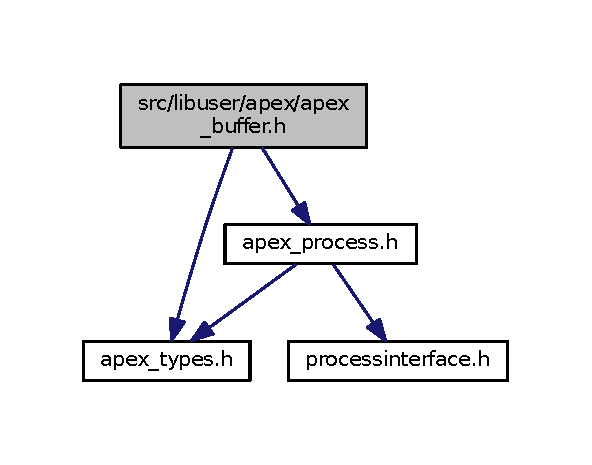
\includegraphics[width=284pt]{apex__buffer_8h__incl}
\end{center}
\end{figure}
This graph shows which files directly or indirectly include this file\+:
\nopagebreak
\begin{figure}[H]
\begin{center}
\leavevmode
\includegraphics[width=198pt]{apex__buffer_8h__dep__incl}
\end{center}
\end{figure}
\subsection*{Classes}
\begin{DoxyCompactItemize}
\item 
struct \hyperlink{structBUFFER__STATUS__TYPE}{B\+U\+F\+F\+E\+R\+\_\+\+S\+T\+A\+T\+U\+S\+\_\+\+T\+Y\+PE}
\end{DoxyCompactItemize}
\subsection*{Macros}
\begin{DoxyCompactItemize}
\item 
\#define \hyperlink{apex__buffer_8h_a3ad5580b78a02dc3d40dc9b359ea540e}{M\+A\+X\+\_\+\+N\+U\+M\+B\+E\+R\+\_\+\+O\+F\+\_\+\+B\+U\+F\+F\+E\+RS}~\hyperlink{apex__types_8h_a29a6a6f7c09a9f0c01d1ba3de83c9380}{S\+Y\+S\+T\+E\+M\+\_\+\+L\+I\+M\+I\+T\+\_\+\+N\+U\+M\+B\+E\+R\+\_\+\+O\+F\+\_\+\+B\+U\+F\+F\+E\+RS}
\end{DoxyCompactItemize}
\subsection*{Typedefs}
\begin{DoxyCompactItemize}
\item 
typedef \hyperlink{structNAME__TYPE}{N\+A\+M\+E\+\_\+\+T\+Y\+PE} \hyperlink{apex__buffer_8h_a9e52e7bf9211d91bd78c498a1b13a082}{B\+U\+F\+F\+E\+R\+\_\+\+N\+A\+M\+E\+\_\+\+T\+Y\+PE}
\item 
typedef \hyperlink{apex__types_8h_a4e13487a80a5740717e19f7f693e06c3}{A\+P\+E\+X\+\_\+\+I\+N\+T\+E\+G\+ER} \hyperlink{apex__buffer_8h_a4d0ef68345e2c0c8407673a785cd6287}{B\+U\+F\+F\+E\+R\+\_\+\+I\+D\+\_\+\+T\+Y\+PE}
\end{DoxyCompactItemize}
\subsection*{Functions}
\begin{DoxyCompactItemize}
\item 
void \hyperlink{apex__buffer_8h_a73a9acc78e4b5e4a02a322f0f5c1de02}{C\+R\+E\+A\+T\+E\+\_\+\+B\+U\+F\+F\+ER} (\hyperlink{apex__buffer_8h_a9e52e7bf9211d91bd78c498a1b13a082}{B\+U\+F\+F\+E\+R\+\_\+\+N\+A\+M\+E\+\_\+\+T\+Y\+PE} B\+U\+F\+F\+E\+R\+\_\+\+N\+A\+ME, \hyperlink{apex__types_8h_ae09494a8d78c38c94f0cc5a80e69785a}{M\+E\+S\+S\+A\+G\+E\+\_\+\+S\+I\+Z\+E\+\_\+\+T\+Y\+PE} M\+A\+X\+\_\+\+M\+E\+S\+S\+A\+G\+E\+\_\+\+S\+I\+ZE, \hyperlink{apex__types_8h_aeffd61fe45ce21b94c1f0b5b84e614ea}{M\+E\+S\+S\+A\+G\+E\+\_\+\+R\+A\+N\+G\+E\+\_\+\+T\+Y\+PE} M\+A\+X\+\_\+\+N\+B\+\_\+\+M\+E\+S\+S\+A\+GE, \hyperlink{apex__types_8h_a35f7a2796e3b68b025d76be6805a1c53}{Q\+U\+E\+U\+I\+N\+G\+\_\+\+D\+I\+S\+C\+I\+P\+L\+I\+N\+E\+\_\+\+T\+Y\+PE} Q\+U\+E\+U\+I\+N\+G\+\_\+\+D\+I\+S\+C\+I\+P\+L\+I\+NE, \hyperlink{apex__buffer_8h_a4d0ef68345e2c0c8407673a785cd6287}{B\+U\+F\+F\+E\+R\+\_\+\+I\+D\+\_\+\+T\+Y\+PE} $\ast$B\+U\+F\+F\+E\+R\+\_\+\+ID, \hyperlink{apex__types_8h_a5cd52791e89e2513bef42ff9193691aa}{R\+E\+T\+U\+R\+N\+\_\+\+C\+O\+D\+E\+\_\+\+T\+Y\+PE} $\ast$R\+E\+T\+U\+R\+N\+\_\+\+C\+O\+DE)
\item 
void \hyperlink{apex__buffer_8h_a109ff9077b123a8a3b9c56b859b011fb}{S\+E\+N\+D\+\_\+\+B\+U\+F\+F\+ER} (\hyperlink{apex__buffer_8h_a4d0ef68345e2c0c8407673a785cd6287}{B\+U\+F\+F\+E\+R\+\_\+\+I\+D\+\_\+\+T\+Y\+PE} B\+U\+F\+F\+E\+R\+\_\+\+ID, \hyperlink{apex__types_8h_a1c9c3acbb8c99c2cbc7751db5226b1fc}{M\+E\+S\+S\+A\+G\+E\+\_\+\+A\+D\+D\+R\+\_\+\+T\+Y\+PE} M\+E\+S\+S\+A\+G\+E\+\_\+\+A\+D\+DR, \hyperlink{apex__types_8h_ae09494a8d78c38c94f0cc5a80e69785a}{M\+E\+S\+S\+A\+G\+E\+\_\+\+S\+I\+Z\+E\+\_\+\+T\+Y\+PE} L\+E\+N\+G\+TH, \hyperlink{apex__types_8h_a78cd52c2621ddf2eda68fcd4bedbc1a7}{S\+Y\+S\+T\+E\+M\+\_\+\+T\+I\+M\+E\+\_\+\+T\+Y\+PE} T\+I\+M\+E\+\_\+\+O\+UT, \hyperlink{apex__types_8h_a5cd52791e89e2513bef42ff9193691aa}{R\+E\+T\+U\+R\+N\+\_\+\+C\+O\+D\+E\+\_\+\+T\+Y\+PE} $\ast$R\+E\+T\+U\+R\+N\+\_\+\+C\+O\+DE)
\item 
void \hyperlink{apex__buffer_8h_a36cea42cc147e18aac25322442c7da31}{R\+E\+C\+E\+I\+V\+E\+\_\+\+B\+U\+F\+F\+ER} (\hyperlink{apex__buffer_8h_a4d0ef68345e2c0c8407673a785cd6287}{B\+U\+F\+F\+E\+R\+\_\+\+I\+D\+\_\+\+T\+Y\+PE} B\+U\+F\+F\+E\+R\+\_\+\+ID, \hyperlink{apex__types_8h_a78cd52c2621ddf2eda68fcd4bedbc1a7}{S\+Y\+S\+T\+E\+M\+\_\+\+T\+I\+M\+E\+\_\+\+T\+Y\+PE} T\+I\+M\+E\+\_\+\+O\+UT, \hyperlink{apex__types_8h_a1c9c3acbb8c99c2cbc7751db5226b1fc}{M\+E\+S\+S\+A\+G\+E\+\_\+\+A\+D\+D\+R\+\_\+\+T\+Y\+PE} M\+E\+S\+S\+A\+G\+E\+\_\+\+A\+D\+DR, \hyperlink{apex__types_8h_ae09494a8d78c38c94f0cc5a80e69785a}{M\+E\+S\+S\+A\+G\+E\+\_\+\+S\+I\+Z\+E\+\_\+\+T\+Y\+PE} $\ast$L\+E\+N\+G\+TH, \hyperlink{apex__types_8h_a5cd52791e89e2513bef42ff9193691aa}{R\+E\+T\+U\+R\+N\+\_\+\+C\+O\+D\+E\+\_\+\+T\+Y\+PE} $\ast$R\+E\+T\+U\+R\+N\+\_\+\+C\+O\+DE)
\item 
void \hyperlink{apex__buffer_8h_ad8b5a7ff36b9b9611215894d0c5bdb33}{G\+E\+T\+\_\+\+B\+U\+F\+F\+E\+R\+\_\+\+ID} (\hyperlink{apex__buffer_8h_a9e52e7bf9211d91bd78c498a1b13a082}{B\+U\+F\+F\+E\+R\+\_\+\+N\+A\+M\+E\+\_\+\+T\+Y\+PE} B\+U\+F\+F\+E\+R\+\_\+\+N\+A\+ME, \hyperlink{apex__buffer_8h_a4d0ef68345e2c0c8407673a785cd6287}{B\+U\+F\+F\+E\+R\+\_\+\+I\+D\+\_\+\+T\+Y\+PE} $\ast$B\+U\+F\+F\+E\+R\+\_\+\+ID, \hyperlink{apex__types_8h_a5cd52791e89e2513bef42ff9193691aa}{R\+E\+T\+U\+R\+N\+\_\+\+C\+O\+D\+E\+\_\+\+T\+Y\+PE} $\ast$R\+E\+T\+U\+R\+N\+\_\+\+C\+O\+DE)
\item 
void \hyperlink{apex__buffer_8h_afd6fd625daee885e062bbd59e548f2a7}{G\+E\+T\+\_\+\+B\+U\+F\+F\+E\+R\+\_\+\+S\+T\+A\+T\+US} (\hyperlink{apex__buffer_8h_a4d0ef68345e2c0c8407673a785cd6287}{B\+U\+F\+F\+E\+R\+\_\+\+I\+D\+\_\+\+T\+Y\+PE} B\+U\+F\+F\+E\+R\+\_\+\+ID, \hyperlink{structBUFFER__STATUS__TYPE}{B\+U\+F\+F\+E\+R\+\_\+\+S\+T\+A\+T\+U\+S\+\_\+\+T\+Y\+PE} $\ast$B\+U\+F\+F\+E\+R\+\_\+\+S\+T\+A\+T\+US, \hyperlink{apex__types_8h_a5cd52791e89e2513bef42ff9193691aa}{R\+E\+T\+U\+R\+N\+\_\+\+C\+O\+D\+E\+\_\+\+T\+Y\+PE} $\ast$R\+E\+T\+U\+R\+N\+\_\+\+C\+O\+DE)
\end{DoxyCompactItemize}


\subsection{Macro Definition Documentation}
\index{apex\+\_\+buffer.\+h@{apex\+\_\+buffer.\+h}!M\+A\+X\+\_\+\+N\+U\+M\+B\+E\+R\+\_\+\+O\+F\+\_\+\+B\+U\+F\+F\+E\+RS@{M\+A\+X\+\_\+\+N\+U\+M\+B\+E\+R\+\_\+\+O\+F\+\_\+\+B\+U\+F\+F\+E\+RS}}
\index{M\+A\+X\+\_\+\+N\+U\+M\+B\+E\+R\+\_\+\+O\+F\+\_\+\+B\+U\+F\+F\+E\+RS@{M\+A\+X\+\_\+\+N\+U\+M\+B\+E\+R\+\_\+\+O\+F\+\_\+\+B\+U\+F\+F\+E\+RS}!apex\+\_\+buffer.\+h@{apex\+\_\+buffer.\+h}}
\subsubsection[{\texorpdfstring{M\+A\+X\+\_\+\+N\+U\+M\+B\+E\+R\+\_\+\+O\+F\+\_\+\+B\+U\+F\+F\+E\+RS}{MAX_NUMBER_OF_BUFFERS}}]{\setlength{\rightskip}{0pt plus 5cm}\#define M\+A\+X\+\_\+\+N\+U\+M\+B\+E\+R\+\_\+\+O\+F\+\_\+\+B\+U\+F\+F\+E\+RS~{\bf S\+Y\+S\+T\+E\+M\+\_\+\+L\+I\+M\+I\+T\+\_\+\+N\+U\+M\+B\+E\+R\+\_\+\+O\+F\+\_\+\+B\+U\+F\+F\+E\+RS}}\hypertarget{apex__buffer_8h_a3ad5580b78a02dc3d40dc9b359ea540e}{}\label{apex__buffer_8h_a3ad5580b78a02dc3d40dc9b359ea540e}


\subsection{Typedef Documentation}
\index{apex\+\_\+buffer.\+h@{apex\+\_\+buffer.\+h}!B\+U\+F\+F\+E\+R\+\_\+\+I\+D\+\_\+\+T\+Y\+PE@{B\+U\+F\+F\+E\+R\+\_\+\+I\+D\+\_\+\+T\+Y\+PE}}
\index{B\+U\+F\+F\+E\+R\+\_\+\+I\+D\+\_\+\+T\+Y\+PE@{B\+U\+F\+F\+E\+R\+\_\+\+I\+D\+\_\+\+T\+Y\+PE}!apex\+\_\+buffer.\+h@{apex\+\_\+buffer.\+h}}
\subsubsection[{\texorpdfstring{B\+U\+F\+F\+E\+R\+\_\+\+I\+D\+\_\+\+T\+Y\+PE}{BUFFER_ID_TYPE}}]{\setlength{\rightskip}{0pt plus 5cm}typedef {\bf A\+P\+E\+X\+\_\+\+I\+N\+T\+E\+G\+ER} {\bf B\+U\+F\+F\+E\+R\+\_\+\+I\+D\+\_\+\+T\+Y\+PE}}\hypertarget{apex__buffer_8h_a4d0ef68345e2c0c8407673a785cd6287}{}\label{apex__buffer_8h_a4d0ef68345e2c0c8407673a785cd6287}
\index{apex\+\_\+buffer.\+h@{apex\+\_\+buffer.\+h}!B\+U\+F\+F\+E\+R\+\_\+\+N\+A\+M\+E\+\_\+\+T\+Y\+PE@{B\+U\+F\+F\+E\+R\+\_\+\+N\+A\+M\+E\+\_\+\+T\+Y\+PE}}
\index{B\+U\+F\+F\+E\+R\+\_\+\+N\+A\+M\+E\+\_\+\+T\+Y\+PE@{B\+U\+F\+F\+E\+R\+\_\+\+N\+A\+M\+E\+\_\+\+T\+Y\+PE}!apex\+\_\+buffer.\+h@{apex\+\_\+buffer.\+h}}
\subsubsection[{\texorpdfstring{B\+U\+F\+F\+E\+R\+\_\+\+N\+A\+M\+E\+\_\+\+T\+Y\+PE}{BUFFER_NAME_TYPE}}]{\setlength{\rightskip}{0pt plus 5cm}typedef {\bf N\+A\+M\+E\+\_\+\+T\+Y\+PE} {\bf B\+U\+F\+F\+E\+R\+\_\+\+N\+A\+M\+E\+\_\+\+T\+Y\+PE}}\hypertarget{apex__buffer_8h_a9e52e7bf9211d91bd78c498a1b13a082}{}\label{apex__buffer_8h_a9e52e7bf9211d91bd78c498a1b13a082}


\subsection{Function Documentation}
\index{apex\+\_\+buffer.\+h@{apex\+\_\+buffer.\+h}!C\+R\+E\+A\+T\+E\+\_\+\+B\+U\+F\+F\+ER@{C\+R\+E\+A\+T\+E\+\_\+\+B\+U\+F\+F\+ER}}
\index{C\+R\+E\+A\+T\+E\+\_\+\+B\+U\+F\+F\+ER@{C\+R\+E\+A\+T\+E\+\_\+\+B\+U\+F\+F\+ER}!apex\+\_\+buffer.\+h@{apex\+\_\+buffer.\+h}}
\subsubsection[{\texorpdfstring{C\+R\+E\+A\+T\+E\+\_\+\+B\+U\+F\+F\+E\+R(\+B\+U\+F\+F\+E\+R\+\_\+\+N\+A\+M\+E\+\_\+\+T\+Y\+P\+E B\+U\+F\+F\+E\+R\+\_\+\+N\+A\+M\+E, M\+E\+S\+S\+A\+G\+E\+\_\+\+S\+I\+Z\+E\+\_\+\+T\+Y\+P\+E M\+A\+X\+\_\+\+M\+E\+S\+S\+A\+G\+E\+\_\+\+S\+I\+Z\+E, M\+E\+S\+S\+A\+G\+E\+\_\+\+R\+A\+N\+G\+E\+\_\+\+T\+Y\+P\+E M\+A\+X\+\_\+\+N\+B\+\_\+\+M\+E\+S\+S\+A\+G\+E, Q\+U\+E\+U\+I\+N\+G\+\_\+\+D\+I\+S\+C\+I\+P\+L\+I\+N\+E\+\_\+\+T\+Y\+P\+E Q\+U\+E\+U\+I\+N\+G\+\_\+\+D\+I\+S\+C\+I\+P\+L\+I\+N\+E, B\+U\+F\+F\+E\+R\+\_\+\+I\+D\+\_\+\+T\+Y\+P\+E $\ast$\+B\+U\+F\+F\+E\+R\+\_\+\+I\+D, R\+E\+T\+U\+R\+N\+\_\+\+C\+O\+D\+E\+\_\+\+T\+Y\+P\+E $\ast$\+R\+E\+T\+U\+R\+N\+\_\+\+C\+O\+D\+E)}{CREATE_BUFFER(BUFFER_NAME_TYPE BUFFER_NAME, MESSAGE_SIZE_TYPE MAX_MESSAGE_SIZE, MESSAGE_RANGE_TYPE MAX_NB_MESSAGE, QUEUING_DISCIPLINE_TYPE QUEUING_DISCIPLINE, BUFFER_ID_TYPE *BUFFER_ID, RETURN_CODE_TYPE *RETURN_CODE)}}]{\setlength{\rightskip}{0pt plus 5cm}void C\+R\+E\+A\+T\+E\+\_\+\+B\+U\+F\+F\+ER (
\begin{DoxyParamCaption}
\item[{{\bf B\+U\+F\+F\+E\+R\+\_\+\+N\+A\+M\+E\+\_\+\+T\+Y\+PE}}]{B\+U\+F\+F\+E\+R\+\_\+\+N\+A\+ME, }
\item[{{\bf M\+E\+S\+S\+A\+G\+E\+\_\+\+S\+I\+Z\+E\+\_\+\+T\+Y\+PE}}]{M\+A\+X\+\_\+\+M\+E\+S\+S\+A\+G\+E\+\_\+\+S\+I\+ZE, }
\item[{{\bf M\+E\+S\+S\+A\+G\+E\+\_\+\+R\+A\+N\+G\+E\+\_\+\+T\+Y\+PE}}]{M\+A\+X\+\_\+\+N\+B\+\_\+\+M\+E\+S\+S\+A\+GE, }
\item[{{\bf Q\+U\+E\+U\+I\+N\+G\+\_\+\+D\+I\+S\+C\+I\+P\+L\+I\+N\+E\+\_\+\+T\+Y\+PE}}]{Q\+U\+E\+U\+I\+N\+G\+\_\+\+D\+I\+S\+C\+I\+P\+L\+I\+NE, }
\item[{{\bf B\+U\+F\+F\+E\+R\+\_\+\+I\+D\+\_\+\+T\+Y\+PE} $\ast$}]{B\+U\+F\+F\+E\+R\+\_\+\+ID, }
\item[{{\bf R\+E\+T\+U\+R\+N\+\_\+\+C\+O\+D\+E\+\_\+\+T\+Y\+PE} $\ast$}]{R\+E\+T\+U\+R\+N\+\_\+\+C\+O\+DE}
\end{DoxyParamCaption}
)}\hypertarget{apex__buffer_8h_a73a9acc78e4b5e4a02a322f0f5c1de02}{}\label{apex__buffer_8h_a73a9acc78e4b5e4a02a322f0f5c1de02}
\index{apex\+\_\+buffer.\+h@{apex\+\_\+buffer.\+h}!G\+E\+T\+\_\+\+B\+U\+F\+F\+E\+R\+\_\+\+ID@{G\+E\+T\+\_\+\+B\+U\+F\+F\+E\+R\+\_\+\+ID}}
\index{G\+E\+T\+\_\+\+B\+U\+F\+F\+E\+R\+\_\+\+ID@{G\+E\+T\+\_\+\+B\+U\+F\+F\+E\+R\+\_\+\+ID}!apex\+\_\+buffer.\+h@{apex\+\_\+buffer.\+h}}
\subsubsection[{\texorpdfstring{G\+E\+T\+\_\+\+B\+U\+F\+F\+E\+R\+\_\+\+I\+D(\+B\+U\+F\+F\+E\+R\+\_\+\+N\+A\+M\+E\+\_\+\+T\+Y\+P\+E B\+U\+F\+F\+E\+R\+\_\+\+N\+A\+M\+E, B\+U\+F\+F\+E\+R\+\_\+\+I\+D\+\_\+\+T\+Y\+P\+E $\ast$\+B\+U\+F\+F\+E\+R\+\_\+\+I\+D, R\+E\+T\+U\+R\+N\+\_\+\+C\+O\+D\+E\+\_\+\+T\+Y\+P\+E $\ast$\+R\+E\+T\+U\+R\+N\+\_\+\+C\+O\+D\+E)}{GET_BUFFER_ID(BUFFER_NAME_TYPE BUFFER_NAME, BUFFER_ID_TYPE *BUFFER_ID, RETURN_CODE_TYPE *RETURN_CODE)}}]{\setlength{\rightskip}{0pt plus 5cm}void G\+E\+T\+\_\+\+B\+U\+F\+F\+E\+R\+\_\+\+ID (
\begin{DoxyParamCaption}
\item[{{\bf B\+U\+F\+F\+E\+R\+\_\+\+N\+A\+M\+E\+\_\+\+T\+Y\+PE}}]{B\+U\+F\+F\+E\+R\+\_\+\+N\+A\+ME, }
\item[{{\bf B\+U\+F\+F\+E\+R\+\_\+\+I\+D\+\_\+\+T\+Y\+PE} $\ast$}]{B\+U\+F\+F\+E\+R\+\_\+\+ID, }
\item[{{\bf R\+E\+T\+U\+R\+N\+\_\+\+C\+O\+D\+E\+\_\+\+T\+Y\+PE} $\ast$}]{R\+E\+T\+U\+R\+N\+\_\+\+C\+O\+DE}
\end{DoxyParamCaption}
)}\hypertarget{apex__buffer_8h_ad8b5a7ff36b9b9611215894d0c5bdb33}{}\label{apex__buffer_8h_ad8b5a7ff36b9b9611215894d0c5bdb33}
\index{apex\+\_\+buffer.\+h@{apex\+\_\+buffer.\+h}!G\+E\+T\+\_\+\+B\+U\+F\+F\+E\+R\+\_\+\+S\+T\+A\+T\+US@{G\+E\+T\+\_\+\+B\+U\+F\+F\+E\+R\+\_\+\+S\+T\+A\+T\+US}}
\index{G\+E\+T\+\_\+\+B\+U\+F\+F\+E\+R\+\_\+\+S\+T\+A\+T\+US@{G\+E\+T\+\_\+\+B\+U\+F\+F\+E\+R\+\_\+\+S\+T\+A\+T\+US}!apex\+\_\+buffer.\+h@{apex\+\_\+buffer.\+h}}
\subsubsection[{\texorpdfstring{G\+E\+T\+\_\+\+B\+U\+F\+F\+E\+R\+\_\+\+S\+T\+A\+T\+U\+S(\+B\+U\+F\+F\+E\+R\+\_\+\+I\+D\+\_\+\+T\+Y\+P\+E B\+U\+F\+F\+E\+R\+\_\+\+I\+D, B\+U\+F\+F\+E\+R\+\_\+\+S\+T\+A\+T\+U\+S\+\_\+\+T\+Y\+P\+E $\ast$\+B\+U\+F\+F\+E\+R\+\_\+\+S\+T\+A\+T\+U\+S, R\+E\+T\+U\+R\+N\+\_\+\+C\+O\+D\+E\+\_\+\+T\+Y\+P\+E $\ast$\+R\+E\+T\+U\+R\+N\+\_\+\+C\+O\+D\+E)}{GET_BUFFER_STATUS(BUFFER_ID_TYPE BUFFER_ID, BUFFER_STATUS_TYPE *BUFFER_STATUS, RETURN_CODE_TYPE *RETURN_CODE)}}]{\setlength{\rightskip}{0pt plus 5cm}void G\+E\+T\+\_\+\+B\+U\+F\+F\+E\+R\+\_\+\+S\+T\+A\+T\+US (
\begin{DoxyParamCaption}
\item[{{\bf B\+U\+F\+F\+E\+R\+\_\+\+I\+D\+\_\+\+T\+Y\+PE}}]{B\+U\+F\+F\+E\+R\+\_\+\+ID, }
\item[{{\bf B\+U\+F\+F\+E\+R\+\_\+\+S\+T\+A\+T\+U\+S\+\_\+\+T\+Y\+PE} $\ast$}]{B\+U\+F\+F\+E\+R\+\_\+\+S\+T\+A\+T\+US, }
\item[{{\bf R\+E\+T\+U\+R\+N\+\_\+\+C\+O\+D\+E\+\_\+\+T\+Y\+PE} $\ast$}]{R\+E\+T\+U\+R\+N\+\_\+\+C\+O\+DE}
\end{DoxyParamCaption}
)}\hypertarget{apex__buffer_8h_afd6fd625daee885e062bbd59e548f2a7}{}\label{apex__buffer_8h_afd6fd625daee885e062bbd59e548f2a7}
\index{apex\+\_\+buffer.\+h@{apex\+\_\+buffer.\+h}!R\+E\+C\+E\+I\+V\+E\+\_\+\+B\+U\+F\+F\+ER@{R\+E\+C\+E\+I\+V\+E\+\_\+\+B\+U\+F\+F\+ER}}
\index{R\+E\+C\+E\+I\+V\+E\+\_\+\+B\+U\+F\+F\+ER@{R\+E\+C\+E\+I\+V\+E\+\_\+\+B\+U\+F\+F\+ER}!apex\+\_\+buffer.\+h@{apex\+\_\+buffer.\+h}}
\subsubsection[{\texorpdfstring{R\+E\+C\+E\+I\+V\+E\+\_\+\+B\+U\+F\+F\+E\+R(\+B\+U\+F\+F\+E\+R\+\_\+\+I\+D\+\_\+\+T\+Y\+P\+E B\+U\+F\+F\+E\+R\+\_\+\+I\+D, S\+Y\+S\+T\+E\+M\+\_\+\+T\+I\+M\+E\+\_\+\+T\+Y\+P\+E T\+I\+M\+E\+\_\+\+O\+U\+T, M\+E\+S\+S\+A\+G\+E\+\_\+\+A\+D\+D\+R\+\_\+\+T\+Y\+P\+E M\+E\+S\+S\+A\+G\+E\+\_\+\+A\+D\+D\+R, M\+E\+S\+S\+A\+G\+E\+\_\+\+S\+I\+Z\+E\+\_\+\+T\+Y\+P\+E $\ast$\+L\+E\+N\+G\+T\+H, R\+E\+T\+U\+R\+N\+\_\+\+C\+O\+D\+E\+\_\+\+T\+Y\+P\+E $\ast$\+R\+E\+T\+U\+R\+N\+\_\+\+C\+O\+D\+E)}{RECEIVE_BUFFER(BUFFER_ID_TYPE BUFFER_ID, SYSTEM_TIME_TYPE TIME_OUT, MESSAGE_ADDR_TYPE MESSAGE_ADDR, MESSAGE_SIZE_TYPE *LENGTH, RETURN_CODE_TYPE *RETURN_CODE)}}]{\setlength{\rightskip}{0pt plus 5cm}void R\+E\+C\+E\+I\+V\+E\+\_\+\+B\+U\+F\+F\+ER (
\begin{DoxyParamCaption}
\item[{{\bf B\+U\+F\+F\+E\+R\+\_\+\+I\+D\+\_\+\+T\+Y\+PE}}]{B\+U\+F\+F\+E\+R\+\_\+\+ID, }
\item[{{\bf S\+Y\+S\+T\+E\+M\+\_\+\+T\+I\+M\+E\+\_\+\+T\+Y\+PE}}]{T\+I\+M\+E\+\_\+\+O\+UT, }
\item[{{\bf M\+E\+S\+S\+A\+G\+E\+\_\+\+A\+D\+D\+R\+\_\+\+T\+Y\+PE}}]{M\+E\+S\+S\+A\+G\+E\+\_\+\+A\+D\+DR, }
\item[{{\bf M\+E\+S\+S\+A\+G\+E\+\_\+\+S\+I\+Z\+E\+\_\+\+T\+Y\+PE} $\ast$}]{L\+E\+N\+G\+TH, }
\item[{{\bf R\+E\+T\+U\+R\+N\+\_\+\+C\+O\+D\+E\+\_\+\+T\+Y\+PE} $\ast$}]{R\+E\+T\+U\+R\+N\+\_\+\+C\+O\+DE}
\end{DoxyParamCaption}
)}\hypertarget{apex__buffer_8h_a36cea42cc147e18aac25322442c7da31}{}\label{apex__buffer_8h_a36cea42cc147e18aac25322442c7da31}
\index{apex\+\_\+buffer.\+h@{apex\+\_\+buffer.\+h}!S\+E\+N\+D\+\_\+\+B\+U\+F\+F\+ER@{S\+E\+N\+D\+\_\+\+B\+U\+F\+F\+ER}}
\index{S\+E\+N\+D\+\_\+\+B\+U\+F\+F\+ER@{S\+E\+N\+D\+\_\+\+B\+U\+F\+F\+ER}!apex\+\_\+buffer.\+h@{apex\+\_\+buffer.\+h}}
\subsubsection[{\texorpdfstring{S\+E\+N\+D\+\_\+\+B\+U\+F\+F\+E\+R(\+B\+U\+F\+F\+E\+R\+\_\+\+I\+D\+\_\+\+T\+Y\+P\+E B\+U\+F\+F\+E\+R\+\_\+\+I\+D, M\+E\+S\+S\+A\+G\+E\+\_\+\+A\+D\+D\+R\+\_\+\+T\+Y\+P\+E M\+E\+S\+S\+A\+G\+E\+\_\+\+A\+D\+D\+R, M\+E\+S\+S\+A\+G\+E\+\_\+\+S\+I\+Z\+E\+\_\+\+T\+Y\+P\+E L\+E\+N\+G\+T\+H, S\+Y\+S\+T\+E\+M\+\_\+\+T\+I\+M\+E\+\_\+\+T\+Y\+P\+E T\+I\+M\+E\+\_\+\+O\+U\+T, R\+E\+T\+U\+R\+N\+\_\+\+C\+O\+D\+E\+\_\+\+T\+Y\+P\+E $\ast$\+R\+E\+T\+U\+R\+N\+\_\+\+C\+O\+D\+E)}{SEND_BUFFER(BUFFER_ID_TYPE BUFFER_ID, MESSAGE_ADDR_TYPE MESSAGE_ADDR, MESSAGE_SIZE_TYPE LENGTH, SYSTEM_TIME_TYPE TIME_OUT, RETURN_CODE_TYPE *RETURN_CODE)}}]{\setlength{\rightskip}{0pt plus 5cm}void S\+E\+N\+D\+\_\+\+B\+U\+F\+F\+ER (
\begin{DoxyParamCaption}
\item[{{\bf B\+U\+F\+F\+E\+R\+\_\+\+I\+D\+\_\+\+T\+Y\+PE}}]{B\+U\+F\+F\+E\+R\+\_\+\+ID, }
\item[{{\bf M\+E\+S\+S\+A\+G\+E\+\_\+\+A\+D\+D\+R\+\_\+\+T\+Y\+PE}}]{M\+E\+S\+S\+A\+G\+E\+\_\+\+A\+D\+DR, }
\item[{{\bf M\+E\+S\+S\+A\+G\+E\+\_\+\+S\+I\+Z\+E\+\_\+\+T\+Y\+PE}}]{L\+E\+N\+G\+TH, }
\item[{{\bf S\+Y\+S\+T\+E\+M\+\_\+\+T\+I\+M\+E\+\_\+\+T\+Y\+PE}}]{T\+I\+M\+E\+\_\+\+O\+UT, }
\item[{{\bf R\+E\+T\+U\+R\+N\+\_\+\+C\+O\+D\+E\+\_\+\+T\+Y\+PE} $\ast$}]{R\+E\+T\+U\+R\+N\+\_\+\+C\+O\+DE}
\end{DoxyParamCaption}
)}\hypertarget{apex__buffer_8h_a109ff9077b123a8a3b9c56b859b011fb}{}\label{apex__buffer_8h_a109ff9077b123a8a3b9c56b859b011fb}

\hypertarget{apex__error_8h}{}\section{src/libuser/apex/apex\+\_\+error.h File Reference}
\label{apex__error_8h}\index{src/libuser/apex/apex\+\_\+error.\+h@{src/libuser/apex/apex\+\_\+error.\+h}}
{\ttfamily \#include \char`\"{}apex\+\_\+process.\+h\char`\"{}}\\*
Include dependency graph for apex\+\_\+error.\+h\+:
\nopagebreak
\begin{figure}[H]
\begin{center}
\leavevmode
\includegraphics[width=284pt]{apex__error_8h__incl}
\end{center}
\end{figure}
This graph shows which files directly or indirectly include this file\+:
\nopagebreak
\begin{figure}[H]
\begin{center}
\leavevmode
\includegraphics[width=350pt]{apex__error_8h__dep__incl}
\end{center}
\end{figure}
\subsection*{Classes}
\begin{DoxyCompactItemize}
\item 
struct \hyperlink{structERROR__STATUS__TYPE}{E\+R\+R\+O\+R\+\_\+\+S\+T\+A\+T\+U\+S\+\_\+\+T\+Y\+PE}
\end{DoxyCompactItemize}
\subsection*{Macros}
\begin{DoxyCompactItemize}
\item 
\#define \hyperlink{apex__error_8h_ab40ad3479d13111f42d84e2cd26c1b13}{M\+A\+X\+\_\+\+E\+R\+R\+O\+R\+\_\+\+M\+E\+S\+S\+A\+G\+E\+\_\+\+S\+I\+ZE}~64
\end{DoxyCompactItemize}
\subsection*{Typedefs}
\begin{DoxyCompactItemize}
\item 
typedef \hyperlink{apex__types_8h_a4e13487a80a5740717e19f7f693e06c3}{A\+P\+E\+X\+\_\+\+I\+N\+T\+E\+G\+ER} \hyperlink{apex__error_8h_a0bec164d28637b1119fe1728e48262c2}{E\+R\+R\+O\+R\+\_\+\+M\+E\+S\+S\+A\+G\+E\+\_\+\+S\+I\+Z\+E\+\_\+\+T\+Y\+PE}
\item 
typedef \hyperlink{apex__types_8h_a762180c8bbb8c9e9229d3e24d25d4dc1}{A\+P\+E\+X\+\_\+\+B\+Y\+TE} \hyperlink{apex__error_8h_a4b70f1f7793b79e3f25032ace3b04ff0}{E\+R\+R\+O\+R\+\_\+\+M\+E\+S\+S\+A\+G\+E\+\_\+\+T\+Y\+PE}\mbox{[}\hyperlink{apex__error_8h_ab40ad3479d13111f42d84e2cd26c1b13}{M\+A\+X\+\_\+\+E\+R\+R\+O\+R\+\_\+\+M\+E\+S\+S\+A\+G\+E\+\_\+\+S\+I\+ZE}\mbox{]}
\end{DoxyCompactItemize}
\subsection*{Enumerations}
\begin{DoxyCompactItemize}
\item 
enum \hyperlink{apex__error_8h_a6c3334fe6390cd6a2e88e6a4aab5ffcc}{E\+R\+R\+O\+R\+\_\+\+C\+O\+D\+E\+\_\+\+T\+Y\+PE} \{ \\*
\hyperlink{apex__error_8h_a6c3334fe6390cd6a2e88e6a4aab5ffccac9836738f9b46d44510d818834b4ce93}{D\+E\+A\+D\+L\+I\+N\+E\+\_\+\+M\+I\+S\+S\+ED} = 0, 
\hyperlink{apex__error_8h_a6c3334fe6390cd6a2e88e6a4aab5ffccabfade3ed8d31c3735a8678a622de2290}{A\+P\+P\+L\+I\+C\+A\+T\+I\+O\+N\+\_\+\+E\+R\+R\+OR} = 1, 
\hyperlink{apex__error_8h_a6c3334fe6390cd6a2e88e6a4aab5ffcca8297e5eb0116a48bc96f44450dab6951}{N\+U\+M\+E\+R\+I\+C\+\_\+\+E\+R\+R\+OR} = 2, 
\hyperlink{apex__error_8h_a6c3334fe6390cd6a2e88e6a4aab5ffcca7dd848f461f96b1df1967ab4264649fa}{I\+L\+L\+E\+G\+A\+L\+\_\+\+R\+E\+Q\+U\+E\+ST} = 3, 
\\*
\hyperlink{apex__error_8h_a6c3334fe6390cd6a2e88e6a4aab5ffcca5ab4c680e2046e128008b8a4bb5e2a59}{S\+T\+A\+C\+K\+\_\+\+O\+V\+E\+R\+F\+L\+OW} = 4, 
\hyperlink{apex__error_8h_a6c3334fe6390cd6a2e88e6a4aab5ffccab247a625c454ddddfe8007f9a9df6648}{M\+E\+M\+O\+R\+Y\+\_\+\+V\+I\+O\+L\+A\+T\+I\+ON} = 5, 
\hyperlink{apex__error_8h_a6c3334fe6390cd6a2e88e6a4aab5ffcca760d3623a0da315d055ec1bd0d462a37}{H\+A\+R\+D\+W\+A\+R\+E\+\_\+\+F\+A\+U\+LT} = 6, 
\hyperlink{apex__error_8h_a6c3334fe6390cd6a2e88e6a4aab5ffcca43016bd5ba6e7cf331c54869a20efdb8}{P\+O\+W\+E\+R\+\_\+\+F\+A\+IL} = 7
 \}
\item 
enum \hyperlink{apex__error_8h_aecf7a2a9c5fb5be7125e5c9eb6d67023}{M\+O\+D\+U\+L\+E\+\_\+\+R\+E\+C\+O\+V\+E\+R\+Y\+\_\+\+A\+C\+T\+I\+O\+N\+\_\+\+T\+Y\+PE} \{ \hyperlink{apex__error_8h_aecf7a2a9c5fb5be7125e5c9eb6d67023a95f1a7f1225304c2d899890044d53011}{I\+G\+N\+O\+RE} = 0, 
\hyperlink{apex__error_8h_aecf7a2a9c5fb5be7125e5c9eb6d67023a7690b021f467450541d8d89123429d40}{S\+H\+U\+T\+D\+O\+WN} = 1, 
\hyperlink{apex__error_8h_aecf7a2a9c5fb5be7125e5c9eb6d67023a589b7d94a3d91d145720e2fed0eb3a05}{R\+E\+S\+ET} = 2
 \}
\item 
enum \hyperlink{apex__error_8h_aa4da4218c0e2dcb8c37ea7a6cb5bd515}{E\+R\+R\+O\+R\+\_\+\+L\+E\+V\+E\+L\+\_\+\+T\+Y\+PE} \{ \hyperlink{apex__error_8h_aa4da4218c0e2dcb8c37ea7a6cb5bd515a89e95e5d1ee3b8077a76005fb143771c}{M\+O\+D\+U\+LE} = 0, 
\hyperlink{apex__error_8h_aa4da4218c0e2dcb8c37ea7a6cb5bd515ac7db78a17d69bcd5f7f6d8a841b57c31}{P\+A\+R\+T\+I\+T\+I\+ON} = 1, 
\hyperlink{apex__error_8h_aa4da4218c0e2dcb8c37ea7a6cb5bd515ae4f21099481eef801603441650cb6eff}{P\+R\+O\+C\+E\+SS} = 2
 \}
\item 
enum \hyperlink{apex__error_8h_ada19fff69e514819fd83d8b3a7fa4e00}{M\+O\+D\+U\+L\+E\+\_\+\+E\+R\+R\+O\+R\+\_\+\+L\+E\+V\+E\+L\+\_\+\+T\+Y\+PE} \{ \hyperlink{apex__error_8h_ada19fff69e514819fd83d8b3a7fa4e00a1cf5e1f5569acda3c4a88a91c5130a69}{M\+O\+D\+U\+L\+E\+\_\+\+E\+R\+R\+O\+R\+\_\+\+L\+E\+V\+E\+L\+\_\+\+T\+Y\+P\+E\+::\+M\+O\+D\+U\+LE}, 
\hyperlink{apex__error_8h_ada19fff69e514819fd83d8b3a7fa4e00a85144455b78d4b11ee8c715122a66694}{M\+O\+D\+U\+L\+E\+\_\+\+E\+R\+R\+O\+R\+\_\+\+L\+E\+V\+E\+L\+\_\+\+T\+Y\+P\+E\+::\+P\+A\+R\+T\+I\+T\+I\+ON}
 \}
\item 
enum \hyperlink{apex__error_8h_a6538eaca68f4beb08798491de78db23e}{P\+A\+R\+T\+I\+T\+I\+O\+N\+\_\+\+E\+R\+R\+O\+R\+\_\+\+L\+E\+V\+E\+L\+\_\+\+T\+Y\+PE} \{ \hyperlink{apex__error_8h_a6538eaca68f4beb08798491de78db23ea85144455b78d4b11ee8c715122a66694}{P\+A\+R\+T\+I\+T\+I\+O\+N\+\_\+\+E\+R\+R\+O\+R\+\_\+\+L\+E\+V\+E\+L\+\_\+\+T\+Y\+P\+E\+::\+P\+A\+R\+T\+I\+T\+I\+ON}, 
\hyperlink{apex__error_8h_a6538eaca68f4beb08798491de78db23eab93c13848c6490ae962feec15fbdd151}{P\+A\+R\+T\+I\+T\+I\+O\+N\+\_\+\+E\+R\+R\+O\+R\+\_\+\+L\+E\+V\+E\+L\+\_\+\+T\+Y\+P\+E\+::\+P\+R\+O\+C\+E\+SS}
 \}
\item 
enum \hyperlink{apex__error_8h_a67c707aa73a83e2566aa9604c01feaa2}{E\+R\+R\+O\+R\+\_\+\+H\+A\+N\+D\+L\+E\+R\+\_\+\+C\+O\+N\+C\+U\+R\+R\+E\+N\+C\+Y\+\_\+\+C\+O\+N\+T\+R\+O\+L\+\_\+\+T\+Y\+PE} \{ \hyperlink{apex__error_8h_a67c707aa73a83e2566aa9604c01feaa2ac977246155478c52e36e1ef3c3ab2654}{P\+R\+O\+C\+E\+S\+S\+\_\+\+P\+A\+U\+SE} = 0, 
\hyperlink{apex__error_8h_a67c707aa73a83e2566aa9604c01feaa2a5123de5a73e899589b53cf95f7d14328}{P\+R\+O\+C\+E\+S\+S\+\_\+\+S\+C\+H\+E\+D\+U\+LE} = 1
 \}
\end{DoxyCompactItemize}
\subsection*{Functions}
\begin{DoxyCompactItemize}
\item 
void \hyperlink{apex__error_8h_afe885350bfeaf05914a6e7eefe026781}{R\+E\+P\+O\+R\+T\+\_\+\+A\+P\+P\+L\+I\+C\+A\+T\+I\+O\+N\+\_\+\+M\+E\+S\+S\+A\+GE} (\hyperlink{apex__types_8h_a1c9c3acbb8c99c2cbc7751db5226b1fc}{M\+E\+S\+S\+A\+G\+E\+\_\+\+A\+D\+D\+R\+\_\+\+T\+Y\+PE} M\+E\+S\+S\+A\+G\+E\+\_\+\+A\+D\+DR, \hyperlink{apex__types_8h_ae09494a8d78c38c94f0cc5a80e69785a}{M\+E\+S\+S\+A\+G\+E\+\_\+\+S\+I\+Z\+E\+\_\+\+T\+Y\+PE} L\+E\+N\+G\+TH, \hyperlink{apex__types_8h_a5cd52791e89e2513bef42ff9193691aa}{R\+E\+T\+U\+R\+N\+\_\+\+C\+O\+D\+E\+\_\+\+T\+Y\+PE} $\ast$R\+E\+T\+U\+R\+N\+\_\+\+C\+O\+DE)
\item 
void \hyperlink{apex__error_8h_a60ead078661a7748ee1b3ef5f2986b70}{C\+R\+E\+A\+T\+E\+\_\+\+E\+R\+R\+O\+R\+\_\+\+H\+A\+N\+D\+L\+ER} (\hyperlink{apex__types_8h_afad87659fcb2bad73146a13b260290b9}{S\+Y\+S\+T\+E\+M\+\_\+\+A\+D\+D\+R\+E\+S\+S\+\_\+\+T\+Y\+PE} E\+N\+T\+R\+Y\+\_\+\+P\+O\+I\+NT, \hyperlink{apex__process_8h_a88a1e60035e9edf9ff430765543659b2}{S\+T\+A\+C\+K\+\_\+\+S\+I\+Z\+E\+\_\+\+T\+Y\+PE} S\+T\+A\+C\+K\+\_\+\+S\+I\+ZE, \hyperlink{apex__types_8h_a5cd52791e89e2513bef42ff9193691aa}{R\+E\+T\+U\+R\+N\+\_\+\+C\+O\+D\+E\+\_\+\+T\+Y\+PE} $\ast$R\+E\+T\+U\+R\+N\+\_\+\+C\+O\+DE)
\item 
void \hyperlink{apex__error_8h_a39817b7a57d3abbffa01da7ac305273a}{G\+E\+T\+\_\+\+E\+R\+R\+O\+R\+\_\+\+S\+T\+A\+T\+US} (\hyperlink{structERROR__STATUS__TYPE}{E\+R\+R\+O\+R\+\_\+\+S\+T\+A\+T\+U\+S\+\_\+\+T\+Y\+PE} $\ast$E\+R\+R\+O\+R\+\_\+\+S\+T\+A\+T\+US, \hyperlink{apex__types_8h_a5cd52791e89e2513bef42ff9193691aa}{R\+E\+T\+U\+R\+N\+\_\+\+C\+O\+D\+E\+\_\+\+T\+Y\+PE} $\ast$R\+E\+T\+U\+R\+N\+\_\+\+C\+O\+DE)
\item 
void \hyperlink{apex__error_8h_a565ad9dd1e8ac8ec1021a18f0041cbe4}{R\+A\+I\+S\+E\+\_\+\+A\+P\+P\+L\+I\+C\+A\+T\+I\+O\+N\+\_\+\+E\+R\+R\+OR} (\hyperlink{apex__error_8h_a6c3334fe6390cd6a2e88e6a4aab5ffcc}{E\+R\+R\+O\+R\+\_\+\+C\+O\+D\+E\+\_\+\+T\+Y\+PE} E\+R\+R\+O\+R\+\_\+\+C\+O\+DE, \hyperlink{apex__types_8h_a1c9c3acbb8c99c2cbc7751db5226b1fc}{M\+E\+S\+S\+A\+G\+E\+\_\+\+A\+D\+D\+R\+\_\+\+T\+Y\+PE} M\+E\+S\+S\+A\+G\+E\+\_\+\+A\+D\+DR, \hyperlink{apex__error_8h_a0bec164d28637b1119fe1728e48262c2}{E\+R\+R\+O\+R\+\_\+\+M\+E\+S\+S\+A\+G\+E\+\_\+\+S\+I\+Z\+E\+\_\+\+T\+Y\+PE} L\+E\+N\+G\+TH, \hyperlink{apex__types_8h_a5cd52791e89e2513bef42ff9193691aa}{R\+E\+T\+U\+R\+N\+\_\+\+C\+O\+D\+E\+\_\+\+T\+Y\+PE} $\ast$R\+E\+T\+U\+R\+N\+\_\+\+C\+O\+DE)
\item 
void \hyperlink{apex__error_8h_a3d52999ea5e54fcc62c8099b07adf51b}{C\+O\+N\+F\+I\+G\+U\+R\+E\+\_\+\+E\+R\+R\+O\+R\+\_\+\+H\+A\+N\+D\+L\+ER} (\hyperlink{apex__error_8h_a67c707aa73a83e2566aa9604c01feaa2}{E\+R\+R\+O\+R\+\_\+\+H\+A\+N\+D\+L\+E\+R\+\_\+\+C\+O\+N\+C\+U\+R\+R\+E\+N\+C\+Y\+\_\+\+C\+O\+N\+T\+R\+O\+L\+\_\+\+T\+Y\+PE} C\+O\+N\+C\+U\+R\+R\+E\+N\+C\+Y\+\_\+\+C\+O\+N\+T\+R\+OL, \hyperlink{apex__types_8h_ac081e44ca764e4d769f88a7f3bbc60de}{P\+R\+O\+C\+E\+S\+S\+O\+R\+\_\+\+C\+O\+R\+E\+\_\+\+I\+D\+\_\+\+T\+Y\+PE} P\+R\+O\+C\+E\+S\+S\+O\+R\+\_\+\+C\+O\+R\+E\+\_\+\+ID, \hyperlink{apex__types_8h_a5cd52791e89e2513bef42ff9193691aa}{R\+E\+T\+U\+R\+N\+\_\+\+C\+O\+D\+E\+\_\+\+T\+Y\+PE} $\ast$R\+E\+T\+U\+R\+N\+\_\+\+C\+O\+DE)
\end{DoxyCompactItemize}


\subsection{Macro Definition Documentation}
\index{apex\+\_\+error.\+h@{apex\+\_\+error.\+h}!M\+A\+X\+\_\+\+E\+R\+R\+O\+R\+\_\+\+M\+E\+S\+S\+A\+G\+E\+\_\+\+S\+I\+ZE@{M\+A\+X\+\_\+\+E\+R\+R\+O\+R\+\_\+\+M\+E\+S\+S\+A\+G\+E\+\_\+\+S\+I\+ZE}}
\index{M\+A\+X\+\_\+\+E\+R\+R\+O\+R\+\_\+\+M\+E\+S\+S\+A\+G\+E\+\_\+\+S\+I\+ZE@{M\+A\+X\+\_\+\+E\+R\+R\+O\+R\+\_\+\+M\+E\+S\+S\+A\+G\+E\+\_\+\+S\+I\+ZE}!apex\+\_\+error.\+h@{apex\+\_\+error.\+h}}
\subsubsection[{\texorpdfstring{M\+A\+X\+\_\+\+E\+R\+R\+O\+R\+\_\+\+M\+E\+S\+S\+A\+G\+E\+\_\+\+S\+I\+ZE}{MAX_ERROR_MESSAGE_SIZE}}]{\setlength{\rightskip}{0pt plus 5cm}\#define M\+A\+X\+\_\+\+E\+R\+R\+O\+R\+\_\+\+M\+E\+S\+S\+A\+G\+E\+\_\+\+S\+I\+ZE~64}\hypertarget{apex__error_8h_ab40ad3479d13111f42d84e2cd26c1b13}{}\label{apex__error_8h_ab40ad3479d13111f42d84e2cd26c1b13}


\subsection{Typedef Documentation}
\index{apex\+\_\+error.\+h@{apex\+\_\+error.\+h}!E\+R\+R\+O\+R\+\_\+\+M\+E\+S\+S\+A\+G\+E\+\_\+\+S\+I\+Z\+E\+\_\+\+T\+Y\+PE@{E\+R\+R\+O\+R\+\_\+\+M\+E\+S\+S\+A\+G\+E\+\_\+\+S\+I\+Z\+E\+\_\+\+T\+Y\+PE}}
\index{E\+R\+R\+O\+R\+\_\+\+M\+E\+S\+S\+A\+G\+E\+\_\+\+S\+I\+Z\+E\+\_\+\+T\+Y\+PE@{E\+R\+R\+O\+R\+\_\+\+M\+E\+S\+S\+A\+G\+E\+\_\+\+S\+I\+Z\+E\+\_\+\+T\+Y\+PE}!apex\+\_\+error.\+h@{apex\+\_\+error.\+h}}
\subsubsection[{\texorpdfstring{E\+R\+R\+O\+R\+\_\+\+M\+E\+S\+S\+A\+G\+E\+\_\+\+S\+I\+Z\+E\+\_\+\+T\+Y\+PE}{ERROR_MESSAGE_SIZE_TYPE}}]{\setlength{\rightskip}{0pt plus 5cm}typedef {\bf A\+P\+E\+X\+\_\+\+I\+N\+T\+E\+G\+ER} {\bf E\+R\+R\+O\+R\+\_\+\+M\+E\+S\+S\+A\+G\+E\+\_\+\+S\+I\+Z\+E\+\_\+\+T\+Y\+PE}}\hypertarget{apex__error_8h_a0bec164d28637b1119fe1728e48262c2}{}\label{apex__error_8h_a0bec164d28637b1119fe1728e48262c2}
\index{apex\+\_\+error.\+h@{apex\+\_\+error.\+h}!E\+R\+R\+O\+R\+\_\+\+M\+E\+S\+S\+A\+G\+E\+\_\+\+T\+Y\+PE@{E\+R\+R\+O\+R\+\_\+\+M\+E\+S\+S\+A\+G\+E\+\_\+\+T\+Y\+PE}}
\index{E\+R\+R\+O\+R\+\_\+\+M\+E\+S\+S\+A\+G\+E\+\_\+\+T\+Y\+PE@{E\+R\+R\+O\+R\+\_\+\+M\+E\+S\+S\+A\+G\+E\+\_\+\+T\+Y\+PE}!apex\+\_\+error.\+h@{apex\+\_\+error.\+h}}
\subsubsection[{\texorpdfstring{E\+R\+R\+O\+R\+\_\+\+M\+E\+S\+S\+A\+G\+E\+\_\+\+T\+Y\+PE}{ERROR_MESSAGE_TYPE}}]{\setlength{\rightskip}{0pt plus 5cm}typedef {\bf A\+P\+E\+X\+\_\+\+B\+Y\+TE} E\+R\+R\+O\+R\+\_\+\+M\+E\+S\+S\+A\+G\+E\+\_\+\+T\+Y\+PE\mbox{[}{\bf M\+A\+X\+\_\+\+E\+R\+R\+O\+R\+\_\+\+M\+E\+S\+S\+A\+G\+E\+\_\+\+S\+I\+ZE}\mbox{]}}\hypertarget{apex__error_8h_a4b70f1f7793b79e3f25032ace3b04ff0}{}\label{apex__error_8h_a4b70f1f7793b79e3f25032ace3b04ff0}


\subsection{Enumeration Type Documentation}
\index{apex\+\_\+error.\+h@{apex\+\_\+error.\+h}!E\+R\+R\+O\+R\+\_\+\+C\+O\+D\+E\+\_\+\+T\+Y\+PE@{E\+R\+R\+O\+R\+\_\+\+C\+O\+D\+E\+\_\+\+T\+Y\+PE}}
\index{E\+R\+R\+O\+R\+\_\+\+C\+O\+D\+E\+\_\+\+T\+Y\+PE@{E\+R\+R\+O\+R\+\_\+\+C\+O\+D\+E\+\_\+\+T\+Y\+PE}!apex\+\_\+error.\+h@{apex\+\_\+error.\+h}}
\subsubsection[{\texorpdfstring{E\+R\+R\+O\+R\+\_\+\+C\+O\+D\+E\+\_\+\+T\+Y\+PE}{ERROR_CODE_TYPE}}]{\setlength{\rightskip}{0pt plus 5cm}enum {\bf E\+R\+R\+O\+R\+\_\+\+C\+O\+D\+E\+\_\+\+T\+Y\+PE}}\hypertarget{apex__error_8h_a6c3334fe6390cd6a2e88e6a4aab5ffcc}{}\label{apex__error_8h_a6c3334fe6390cd6a2e88e6a4aab5ffcc}
\begin{Desc}
\item[Enumerator]\par
\begin{description}
\index{D\+E\+A\+D\+L\+I\+N\+E\+\_\+\+M\+I\+S\+S\+ED@{D\+E\+A\+D\+L\+I\+N\+E\+\_\+\+M\+I\+S\+S\+ED}!apex\+\_\+error.\+h@{apex\+\_\+error.\+h}}\index{apex\+\_\+error.\+h@{apex\+\_\+error.\+h}!D\+E\+A\+D\+L\+I\+N\+E\+\_\+\+M\+I\+S\+S\+ED@{D\+E\+A\+D\+L\+I\+N\+E\+\_\+\+M\+I\+S\+S\+ED}}\item[{\em 
D\+E\+A\+D\+L\+I\+N\+E\+\_\+\+M\+I\+S\+S\+ED\hypertarget{apex__error_8h_a6c3334fe6390cd6a2e88e6a4aab5ffccac9836738f9b46d44510d818834b4ce93}{}\label{apex__error_8h_a6c3334fe6390cd6a2e88e6a4aab5ffccac9836738f9b46d44510d818834b4ce93}
}]\index{A\+P\+P\+L\+I\+C\+A\+T\+I\+O\+N\+\_\+\+E\+R\+R\+OR@{A\+P\+P\+L\+I\+C\+A\+T\+I\+O\+N\+\_\+\+E\+R\+R\+OR}!apex\+\_\+error.\+h@{apex\+\_\+error.\+h}}\index{apex\+\_\+error.\+h@{apex\+\_\+error.\+h}!A\+P\+P\+L\+I\+C\+A\+T\+I\+O\+N\+\_\+\+E\+R\+R\+OR@{A\+P\+P\+L\+I\+C\+A\+T\+I\+O\+N\+\_\+\+E\+R\+R\+OR}}\item[{\em 
A\+P\+P\+L\+I\+C\+A\+T\+I\+O\+N\+\_\+\+E\+R\+R\+OR\hypertarget{apex__error_8h_a6c3334fe6390cd6a2e88e6a4aab5ffccabfade3ed8d31c3735a8678a622de2290}{}\label{apex__error_8h_a6c3334fe6390cd6a2e88e6a4aab5ffccabfade3ed8d31c3735a8678a622de2290}
}]\index{N\+U\+M\+E\+R\+I\+C\+\_\+\+E\+R\+R\+OR@{N\+U\+M\+E\+R\+I\+C\+\_\+\+E\+R\+R\+OR}!apex\+\_\+error.\+h@{apex\+\_\+error.\+h}}\index{apex\+\_\+error.\+h@{apex\+\_\+error.\+h}!N\+U\+M\+E\+R\+I\+C\+\_\+\+E\+R\+R\+OR@{N\+U\+M\+E\+R\+I\+C\+\_\+\+E\+R\+R\+OR}}\item[{\em 
N\+U\+M\+E\+R\+I\+C\+\_\+\+E\+R\+R\+OR\hypertarget{apex__error_8h_a6c3334fe6390cd6a2e88e6a4aab5ffcca8297e5eb0116a48bc96f44450dab6951}{}\label{apex__error_8h_a6c3334fe6390cd6a2e88e6a4aab5ffcca8297e5eb0116a48bc96f44450dab6951}
}]\index{I\+L\+L\+E\+G\+A\+L\+\_\+\+R\+E\+Q\+U\+E\+ST@{I\+L\+L\+E\+G\+A\+L\+\_\+\+R\+E\+Q\+U\+E\+ST}!apex\+\_\+error.\+h@{apex\+\_\+error.\+h}}\index{apex\+\_\+error.\+h@{apex\+\_\+error.\+h}!I\+L\+L\+E\+G\+A\+L\+\_\+\+R\+E\+Q\+U\+E\+ST@{I\+L\+L\+E\+G\+A\+L\+\_\+\+R\+E\+Q\+U\+E\+ST}}\item[{\em 
I\+L\+L\+E\+G\+A\+L\+\_\+\+R\+E\+Q\+U\+E\+ST\hypertarget{apex__error_8h_a6c3334fe6390cd6a2e88e6a4aab5ffcca7dd848f461f96b1df1967ab4264649fa}{}\label{apex__error_8h_a6c3334fe6390cd6a2e88e6a4aab5ffcca7dd848f461f96b1df1967ab4264649fa}
}]\index{S\+T\+A\+C\+K\+\_\+\+O\+V\+E\+R\+F\+L\+OW@{S\+T\+A\+C\+K\+\_\+\+O\+V\+E\+R\+F\+L\+OW}!apex\+\_\+error.\+h@{apex\+\_\+error.\+h}}\index{apex\+\_\+error.\+h@{apex\+\_\+error.\+h}!S\+T\+A\+C\+K\+\_\+\+O\+V\+E\+R\+F\+L\+OW@{S\+T\+A\+C\+K\+\_\+\+O\+V\+E\+R\+F\+L\+OW}}\item[{\em 
S\+T\+A\+C\+K\+\_\+\+O\+V\+E\+R\+F\+L\+OW\hypertarget{apex__error_8h_a6c3334fe6390cd6a2e88e6a4aab5ffcca5ab4c680e2046e128008b8a4bb5e2a59}{}\label{apex__error_8h_a6c3334fe6390cd6a2e88e6a4aab5ffcca5ab4c680e2046e128008b8a4bb5e2a59}
}]\index{M\+E\+M\+O\+R\+Y\+\_\+\+V\+I\+O\+L\+A\+T\+I\+ON@{M\+E\+M\+O\+R\+Y\+\_\+\+V\+I\+O\+L\+A\+T\+I\+ON}!apex\+\_\+error.\+h@{apex\+\_\+error.\+h}}\index{apex\+\_\+error.\+h@{apex\+\_\+error.\+h}!M\+E\+M\+O\+R\+Y\+\_\+\+V\+I\+O\+L\+A\+T\+I\+ON@{M\+E\+M\+O\+R\+Y\+\_\+\+V\+I\+O\+L\+A\+T\+I\+ON}}\item[{\em 
M\+E\+M\+O\+R\+Y\+\_\+\+V\+I\+O\+L\+A\+T\+I\+ON\hypertarget{apex__error_8h_a6c3334fe6390cd6a2e88e6a4aab5ffccab247a625c454ddddfe8007f9a9df6648}{}\label{apex__error_8h_a6c3334fe6390cd6a2e88e6a4aab5ffccab247a625c454ddddfe8007f9a9df6648}
}]\index{H\+A\+R\+D\+W\+A\+R\+E\+\_\+\+F\+A\+U\+LT@{H\+A\+R\+D\+W\+A\+R\+E\+\_\+\+F\+A\+U\+LT}!apex\+\_\+error.\+h@{apex\+\_\+error.\+h}}\index{apex\+\_\+error.\+h@{apex\+\_\+error.\+h}!H\+A\+R\+D\+W\+A\+R\+E\+\_\+\+F\+A\+U\+LT@{H\+A\+R\+D\+W\+A\+R\+E\+\_\+\+F\+A\+U\+LT}}\item[{\em 
H\+A\+R\+D\+W\+A\+R\+E\+\_\+\+F\+A\+U\+LT\hypertarget{apex__error_8h_a6c3334fe6390cd6a2e88e6a4aab5ffcca760d3623a0da315d055ec1bd0d462a37}{}\label{apex__error_8h_a6c3334fe6390cd6a2e88e6a4aab5ffcca760d3623a0da315d055ec1bd0d462a37}
}]\index{P\+O\+W\+E\+R\+\_\+\+F\+A\+IL@{P\+O\+W\+E\+R\+\_\+\+F\+A\+IL}!apex\+\_\+error.\+h@{apex\+\_\+error.\+h}}\index{apex\+\_\+error.\+h@{apex\+\_\+error.\+h}!P\+O\+W\+E\+R\+\_\+\+F\+A\+IL@{P\+O\+W\+E\+R\+\_\+\+F\+A\+IL}}\item[{\em 
P\+O\+W\+E\+R\+\_\+\+F\+A\+IL\hypertarget{apex__error_8h_a6c3334fe6390cd6a2e88e6a4aab5ffcca43016bd5ba6e7cf331c54869a20efdb8}{}\label{apex__error_8h_a6c3334fe6390cd6a2e88e6a4aab5ffcca43016bd5ba6e7cf331c54869a20efdb8}
}]\end{description}
\end{Desc}
\index{apex\+\_\+error.\+h@{apex\+\_\+error.\+h}!E\+R\+R\+O\+R\+\_\+\+H\+A\+N\+D\+L\+E\+R\+\_\+\+C\+O\+N\+C\+U\+R\+R\+E\+N\+C\+Y\+\_\+\+C\+O\+N\+T\+R\+O\+L\+\_\+\+T\+Y\+PE@{E\+R\+R\+O\+R\+\_\+\+H\+A\+N\+D\+L\+E\+R\+\_\+\+C\+O\+N\+C\+U\+R\+R\+E\+N\+C\+Y\+\_\+\+C\+O\+N\+T\+R\+O\+L\+\_\+\+T\+Y\+PE}}
\index{E\+R\+R\+O\+R\+\_\+\+H\+A\+N\+D\+L\+E\+R\+\_\+\+C\+O\+N\+C\+U\+R\+R\+E\+N\+C\+Y\+\_\+\+C\+O\+N\+T\+R\+O\+L\+\_\+\+T\+Y\+PE@{E\+R\+R\+O\+R\+\_\+\+H\+A\+N\+D\+L\+E\+R\+\_\+\+C\+O\+N\+C\+U\+R\+R\+E\+N\+C\+Y\+\_\+\+C\+O\+N\+T\+R\+O\+L\+\_\+\+T\+Y\+PE}!apex\+\_\+error.\+h@{apex\+\_\+error.\+h}}
\subsubsection[{\texorpdfstring{E\+R\+R\+O\+R\+\_\+\+H\+A\+N\+D\+L\+E\+R\+\_\+\+C\+O\+N\+C\+U\+R\+R\+E\+N\+C\+Y\+\_\+\+C\+O\+N\+T\+R\+O\+L\+\_\+\+T\+Y\+PE}{ERROR_HANDLER_CONCURRENCY_CONTROL_TYPE}}]{\setlength{\rightskip}{0pt plus 5cm}enum {\bf E\+R\+R\+O\+R\+\_\+\+H\+A\+N\+D\+L\+E\+R\+\_\+\+C\+O\+N\+C\+U\+R\+R\+E\+N\+C\+Y\+\_\+\+C\+O\+N\+T\+R\+O\+L\+\_\+\+T\+Y\+PE}}\hypertarget{apex__error_8h_a67c707aa73a83e2566aa9604c01feaa2}{}\label{apex__error_8h_a67c707aa73a83e2566aa9604c01feaa2}
\begin{Desc}
\item[Enumerator]\par
\begin{description}
\index{P\+R\+O\+C\+E\+S\+S\+\_\+\+P\+A\+U\+SE@{P\+R\+O\+C\+E\+S\+S\+\_\+\+P\+A\+U\+SE}!apex\+\_\+error.\+h@{apex\+\_\+error.\+h}}\index{apex\+\_\+error.\+h@{apex\+\_\+error.\+h}!P\+R\+O\+C\+E\+S\+S\+\_\+\+P\+A\+U\+SE@{P\+R\+O\+C\+E\+S\+S\+\_\+\+P\+A\+U\+SE}}\item[{\em 
P\+R\+O\+C\+E\+S\+S\+\_\+\+P\+A\+U\+SE\hypertarget{apex__error_8h_a67c707aa73a83e2566aa9604c01feaa2ac977246155478c52e36e1ef3c3ab2654}{}\label{apex__error_8h_a67c707aa73a83e2566aa9604c01feaa2ac977246155478c52e36e1ef3c3ab2654}
}]\index{P\+R\+O\+C\+E\+S\+S\+\_\+\+S\+C\+H\+E\+D\+U\+LE@{P\+R\+O\+C\+E\+S\+S\+\_\+\+S\+C\+H\+E\+D\+U\+LE}!apex\+\_\+error.\+h@{apex\+\_\+error.\+h}}\index{apex\+\_\+error.\+h@{apex\+\_\+error.\+h}!P\+R\+O\+C\+E\+S\+S\+\_\+\+S\+C\+H\+E\+D\+U\+LE@{P\+R\+O\+C\+E\+S\+S\+\_\+\+S\+C\+H\+E\+D\+U\+LE}}\item[{\em 
P\+R\+O\+C\+E\+S\+S\+\_\+\+S\+C\+H\+E\+D\+U\+LE\hypertarget{apex__error_8h_a67c707aa73a83e2566aa9604c01feaa2a5123de5a73e899589b53cf95f7d14328}{}\label{apex__error_8h_a67c707aa73a83e2566aa9604c01feaa2a5123de5a73e899589b53cf95f7d14328}
}]\end{description}
\end{Desc}
\index{apex\+\_\+error.\+h@{apex\+\_\+error.\+h}!E\+R\+R\+O\+R\+\_\+\+L\+E\+V\+E\+L\+\_\+\+T\+Y\+PE@{E\+R\+R\+O\+R\+\_\+\+L\+E\+V\+E\+L\+\_\+\+T\+Y\+PE}}
\index{E\+R\+R\+O\+R\+\_\+\+L\+E\+V\+E\+L\+\_\+\+T\+Y\+PE@{E\+R\+R\+O\+R\+\_\+\+L\+E\+V\+E\+L\+\_\+\+T\+Y\+PE}!apex\+\_\+error.\+h@{apex\+\_\+error.\+h}}
\subsubsection[{\texorpdfstring{E\+R\+R\+O\+R\+\_\+\+L\+E\+V\+E\+L\+\_\+\+T\+Y\+PE}{ERROR_LEVEL_TYPE}}]{\setlength{\rightskip}{0pt plus 5cm}enum {\bf E\+R\+R\+O\+R\+\_\+\+L\+E\+V\+E\+L\+\_\+\+T\+Y\+PE}}\hypertarget{apex__error_8h_aa4da4218c0e2dcb8c37ea7a6cb5bd515}{}\label{apex__error_8h_aa4da4218c0e2dcb8c37ea7a6cb5bd515}
\begin{Desc}
\item[Enumerator]\par
\begin{description}
\index{M\+O\+D\+U\+LE@{M\+O\+D\+U\+LE}!apex\+\_\+error.\+h@{apex\+\_\+error.\+h}}\index{apex\+\_\+error.\+h@{apex\+\_\+error.\+h}!M\+O\+D\+U\+LE@{M\+O\+D\+U\+LE}}\item[{\em 
M\+O\+D\+U\+LE\hypertarget{apex__error_8h_aa4da4218c0e2dcb8c37ea7a6cb5bd515a89e95e5d1ee3b8077a76005fb143771c}{}\label{apex__error_8h_aa4da4218c0e2dcb8c37ea7a6cb5bd515a89e95e5d1ee3b8077a76005fb143771c}
}]\index{P\+A\+R\+T\+I\+T\+I\+ON@{P\+A\+R\+T\+I\+T\+I\+ON}!apex\+\_\+error.\+h@{apex\+\_\+error.\+h}}\index{apex\+\_\+error.\+h@{apex\+\_\+error.\+h}!P\+A\+R\+T\+I\+T\+I\+ON@{P\+A\+R\+T\+I\+T\+I\+ON}}\item[{\em 
P\+A\+R\+T\+I\+T\+I\+ON\hypertarget{apex__error_8h_aa4da4218c0e2dcb8c37ea7a6cb5bd515ac7db78a17d69bcd5f7f6d8a841b57c31}{}\label{apex__error_8h_aa4da4218c0e2dcb8c37ea7a6cb5bd515ac7db78a17d69bcd5f7f6d8a841b57c31}
}]\index{P\+R\+O\+C\+E\+SS@{P\+R\+O\+C\+E\+SS}!apex\+\_\+error.\+h@{apex\+\_\+error.\+h}}\index{apex\+\_\+error.\+h@{apex\+\_\+error.\+h}!P\+R\+O\+C\+E\+SS@{P\+R\+O\+C\+E\+SS}}\item[{\em 
P\+R\+O\+C\+E\+SS\hypertarget{apex__error_8h_aa4da4218c0e2dcb8c37ea7a6cb5bd515ae4f21099481eef801603441650cb6eff}{}\label{apex__error_8h_aa4da4218c0e2dcb8c37ea7a6cb5bd515ae4f21099481eef801603441650cb6eff}
}]\end{description}
\end{Desc}
\index{apex\+\_\+error.\+h@{apex\+\_\+error.\+h}!M\+O\+D\+U\+L\+E\+\_\+\+E\+R\+R\+O\+R\+\_\+\+L\+E\+V\+E\+L\+\_\+\+T\+Y\+PE@{M\+O\+D\+U\+L\+E\+\_\+\+E\+R\+R\+O\+R\+\_\+\+L\+E\+V\+E\+L\+\_\+\+T\+Y\+PE}}
\index{M\+O\+D\+U\+L\+E\+\_\+\+E\+R\+R\+O\+R\+\_\+\+L\+E\+V\+E\+L\+\_\+\+T\+Y\+PE@{M\+O\+D\+U\+L\+E\+\_\+\+E\+R\+R\+O\+R\+\_\+\+L\+E\+V\+E\+L\+\_\+\+T\+Y\+PE}!apex\+\_\+error.\+h@{apex\+\_\+error.\+h}}
\subsubsection[{\texorpdfstring{M\+O\+D\+U\+L\+E\+\_\+\+E\+R\+R\+O\+R\+\_\+\+L\+E\+V\+E\+L\+\_\+\+T\+Y\+PE}{MODULE_ERROR_LEVEL_TYPE}}]{\setlength{\rightskip}{0pt plus 5cm}enum {\bf M\+O\+D\+U\+L\+E\+\_\+\+E\+R\+R\+O\+R\+\_\+\+L\+E\+V\+E\+L\+\_\+\+T\+Y\+PE}\hspace{0.3cm}{\ttfamily [strong]}}\hypertarget{apex__error_8h_ada19fff69e514819fd83d8b3a7fa4e00}{}\label{apex__error_8h_ada19fff69e514819fd83d8b3a7fa4e00}
\begin{Desc}
\item[Enumerator]\par
\begin{description}
\index{M\+O\+D\+U\+LE@{M\+O\+D\+U\+LE}!apex\+\_\+error.\+h@{apex\+\_\+error.\+h}}\index{apex\+\_\+error.\+h@{apex\+\_\+error.\+h}!M\+O\+D\+U\+LE@{M\+O\+D\+U\+LE}}\item[{\em 
M\+O\+D\+U\+LE\hypertarget{apex__error_8h_ada19fff69e514819fd83d8b3a7fa4e00a1cf5e1f5569acda3c4a88a91c5130a69}{}\label{apex__error_8h_ada19fff69e514819fd83d8b3a7fa4e00a1cf5e1f5569acda3c4a88a91c5130a69}
}]\index{P\+A\+R\+T\+I\+T\+I\+ON@{P\+A\+R\+T\+I\+T\+I\+ON}!apex\+\_\+error.\+h@{apex\+\_\+error.\+h}}\index{apex\+\_\+error.\+h@{apex\+\_\+error.\+h}!P\+A\+R\+T\+I\+T\+I\+ON@{P\+A\+R\+T\+I\+T\+I\+ON}}\item[{\em 
P\+A\+R\+T\+I\+T\+I\+ON\hypertarget{apex__error_8h_ada19fff69e514819fd83d8b3a7fa4e00a85144455b78d4b11ee8c715122a66694}{}\label{apex__error_8h_ada19fff69e514819fd83d8b3a7fa4e00a85144455b78d4b11ee8c715122a66694}
}]\end{description}
\end{Desc}
\index{apex\+\_\+error.\+h@{apex\+\_\+error.\+h}!M\+O\+D\+U\+L\+E\+\_\+\+R\+E\+C\+O\+V\+E\+R\+Y\+\_\+\+A\+C\+T\+I\+O\+N\+\_\+\+T\+Y\+PE@{M\+O\+D\+U\+L\+E\+\_\+\+R\+E\+C\+O\+V\+E\+R\+Y\+\_\+\+A\+C\+T\+I\+O\+N\+\_\+\+T\+Y\+PE}}
\index{M\+O\+D\+U\+L\+E\+\_\+\+R\+E\+C\+O\+V\+E\+R\+Y\+\_\+\+A\+C\+T\+I\+O\+N\+\_\+\+T\+Y\+PE@{M\+O\+D\+U\+L\+E\+\_\+\+R\+E\+C\+O\+V\+E\+R\+Y\+\_\+\+A\+C\+T\+I\+O\+N\+\_\+\+T\+Y\+PE}!apex\+\_\+error.\+h@{apex\+\_\+error.\+h}}
\subsubsection[{\texorpdfstring{M\+O\+D\+U\+L\+E\+\_\+\+R\+E\+C\+O\+V\+E\+R\+Y\+\_\+\+A\+C\+T\+I\+O\+N\+\_\+\+T\+Y\+PE}{MODULE_RECOVERY_ACTION_TYPE}}]{\setlength{\rightskip}{0pt plus 5cm}enum {\bf M\+O\+D\+U\+L\+E\+\_\+\+R\+E\+C\+O\+V\+E\+R\+Y\+\_\+\+A\+C\+T\+I\+O\+N\+\_\+\+T\+Y\+PE}}\hypertarget{apex__error_8h_aecf7a2a9c5fb5be7125e5c9eb6d67023}{}\label{apex__error_8h_aecf7a2a9c5fb5be7125e5c9eb6d67023}
\begin{Desc}
\item[Enumerator]\par
\begin{description}
\index{I\+G\+N\+O\+RE@{I\+G\+N\+O\+RE}!apex\+\_\+error.\+h@{apex\+\_\+error.\+h}}\index{apex\+\_\+error.\+h@{apex\+\_\+error.\+h}!I\+G\+N\+O\+RE@{I\+G\+N\+O\+RE}}\item[{\em 
I\+G\+N\+O\+RE\hypertarget{apex__error_8h_aecf7a2a9c5fb5be7125e5c9eb6d67023a95f1a7f1225304c2d899890044d53011}{}\label{apex__error_8h_aecf7a2a9c5fb5be7125e5c9eb6d67023a95f1a7f1225304c2d899890044d53011}
}]\index{S\+H\+U\+T\+D\+O\+WN@{S\+H\+U\+T\+D\+O\+WN}!apex\+\_\+error.\+h@{apex\+\_\+error.\+h}}\index{apex\+\_\+error.\+h@{apex\+\_\+error.\+h}!S\+H\+U\+T\+D\+O\+WN@{S\+H\+U\+T\+D\+O\+WN}}\item[{\em 
S\+H\+U\+T\+D\+O\+WN\hypertarget{apex__error_8h_aecf7a2a9c5fb5be7125e5c9eb6d67023a7690b021f467450541d8d89123429d40}{}\label{apex__error_8h_aecf7a2a9c5fb5be7125e5c9eb6d67023a7690b021f467450541d8d89123429d40}
}]\index{R\+E\+S\+ET@{R\+E\+S\+ET}!apex\+\_\+error.\+h@{apex\+\_\+error.\+h}}\index{apex\+\_\+error.\+h@{apex\+\_\+error.\+h}!R\+E\+S\+ET@{R\+E\+S\+ET}}\item[{\em 
R\+E\+S\+ET\hypertarget{apex__error_8h_aecf7a2a9c5fb5be7125e5c9eb6d67023a589b7d94a3d91d145720e2fed0eb3a05}{}\label{apex__error_8h_aecf7a2a9c5fb5be7125e5c9eb6d67023a589b7d94a3d91d145720e2fed0eb3a05}
}]\end{description}
\end{Desc}
\index{apex\+\_\+error.\+h@{apex\+\_\+error.\+h}!P\+A\+R\+T\+I\+T\+I\+O\+N\+\_\+\+E\+R\+R\+O\+R\+\_\+\+L\+E\+V\+E\+L\+\_\+\+T\+Y\+PE@{P\+A\+R\+T\+I\+T\+I\+O\+N\+\_\+\+E\+R\+R\+O\+R\+\_\+\+L\+E\+V\+E\+L\+\_\+\+T\+Y\+PE}}
\index{P\+A\+R\+T\+I\+T\+I\+O\+N\+\_\+\+E\+R\+R\+O\+R\+\_\+\+L\+E\+V\+E\+L\+\_\+\+T\+Y\+PE@{P\+A\+R\+T\+I\+T\+I\+O\+N\+\_\+\+E\+R\+R\+O\+R\+\_\+\+L\+E\+V\+E\+L\+\_\+\+T\+Y\+PE}!apex\+\_\+error.\+h@{apex\+\_\+error.\+h}}
\subsubsection[{\texorpdfstring{P\+A\+R\+T\+I\+T\+I\+O\+N\+\_\+\+E\+R\+R\+O\+R\+\_\+\+L\+E\+V\+E\+L\+\_\+\+T\+Y\+PE}{PARTITION_ERROR_LEVEL_TYPE}}]{\setlength{\rightskip}{0pt plus 5cm}enum {\bf P\+A\+R\+T\+I\+T\+I\+O\+N\+\_\+\+E\+R\+R\+O\+R\+\_\+\+L\+E\+V\+E\+L\+\_\+\+T\+Y\+PE}\hspace{0.3cm}{\ttfamily [strong]}}\hypertarget{apex__error_8h_a6538eaca68f4beb08798491de78db23e}{}\label{apex__error_8h_a6538eaca68f4beb08798491de78db23e}
\begin{Desc}
\item[Enumerator]\par
\begin{description}
\index{P\+A\+R\+T\+I\+T\+I\+ON@{P\+A\+R\+T\+I\+T\+I\+ON}!apex\+\_\+error.\+h@{apex\+\_\+error.\+h}}\index{apex\+\_\+error.\+h@{apex\+\_\+error.\+h}!P\+A\+R\+T\+I\+T\+I\+ON@{P\+A\+R\+T\+I\+T\+I\+ON}}\item[{\em 
P\+A\+R\+T\+I\+T\+I\+ON\hypertarget{apex__error_8h_a6538eaca68f4beb08798491de78db23ea85144455b78d4b11ee8c715122a66694}{}\label{apex__error_8h_a6538eaca68f4beb08798491de78db23ea85144455b78d4b11ee8c715122a66694}
}]\index{P\+R\+O\+C\+E\+SS@{P\+R\+O\+C\+E\+SS}!apex\+\_\+error.\+h@{apex\+\_\+error.\+h}}\index{apex\+\_\+error.\+h@{apex\+\_\+error.\+h}!P\+R\+O\+C\+E\+SS@{P\+R\+O\+C\+E\+SS}}\item[{\em 
P\+R\+O\+C\+E\+SS\hypertarget{apex__error_8h_a6538eaca68f4beb08798491de78db23eab93c13848c6490ae962feec15fbdd151}{}\label{apex__error_8h_a6538eaca68f4beb08798491de78db23eab93c13848c6490ae962feec15fbdd151}
}]\end{description}
\end{Desc}


\subsection{Function Documentation}
\index{apex\+\_\+error.\+h@{apex\+\_\+error.\+h}!C\+O\+N\+F\+I\+G\+U\+R\+E\+\_\+\+E\+R\+R\+O\+R\+\_\+\+H\+A\+N\+D\+L\+ER@{C\+O\+N\+F\+I\+G\+U\+R\+E\+\_\+\+E\+R\+R\+O\+R\+\_\+\+H\+A\+N\+D\+L\+ER}}
\index{C\+O\+N\+F\+I\+G\+U\+R\+E\+\_\+\+E\+R\+R\+O\+R\+\_\+\+H\+A\+N\+D\+L\+ER@{C\+O\+N\+F\+I\+G\+U\+R\+E\+\_\+\+E\+R\+R\+O\+R\+\_\+\+H\+A\+N\+D\+L\+ER}!apex\+\_\+error.\+h@{apex\+\_\+error.\+h}}
\subsubsection[{\texorpdfstring{C\+O\+N\+F\+I\+G\+U\+R\+E\+\_\+\+E\+R\+R\+O\+R\+\_\+\+H\+A\+N\+D\+L\+E\+R(\+E\+R\+R\+O\+R\+\_\+\+H\+A\+N\+D\+L\+E\+R\+\_\+\+C\+O\+N\+C\+U\+R\+R\+E\+N\+C\+Y\+\_\+\+C\+O\+N\+T\+R\+O\+L\+\_\+\+T\+Y\+P\+E C\+O\+N\+C\+U\+R\+R\+E\+N\+C\+Y\+\_\+\+C\+O\+N\+T\+R\+O\+L, P\+R\+O\+C\+E\+S\+S\+O\+R\+\_\+\+C\+O\+R\+E\+\_\+\+I\+D\+\_\+\+T\+Y\+P\+E P\+R\+O\+C\+E\+S\+S\+O\+R\+\_\+\+C\+O\+R\+E\+\_\+\+I\+D, R\+E\+T\+U\+R\+N\+\_\+\+C\+O\+D\+E\+\_\+\+T\+Y\+P\+E $\ast$\+R\+E\+T\+U\+R\+N\+\_\+\+C\+O\+D\+E)}{CONFIGURE_ERROR_HANDLER(ERROR_HANDLER_CONCURRENCY_CONTROL_TYPE CONCURRENCY_CONTROL, PROCESSOR_CORE_ID_TYPE PROCESSOR_CORE_ID, RETURN_CODE_TYPE *RETURN_CODE)}}]{\setlength{\rightskip}{0pt plus 5cm}void C\+O\+N\+F\+I\+G\+U\+R\+E\+\_\+\+E\+R\+R\+O\+R\+\_\+\+H\+A\+N\+D\+L\+ER (
\begin{DoxyParamCaption}
\item[{{\bf E\+R\+R\+O\+R\+\_\+\+H\+A\+N\+D\+L\+E\+R\+\_\+\+C\+O\+N\+C\+U\+R\+R\+E\+N\+C\+Y\+\_\+\+C\+O\+N\+T\+R\+O\+L\+\_\+\+T\+Y\+PE}}]{C\+O\+N\+C\+U\+R\+R\+E\+N\+C\+Y\+\_\+\+C\+O\+N\+T\+R\+OL, }
\item[{{\bf P\+R\+O\+C\+E\+S\+S\+O\+R\+\_\+\+C\+O\+R\+E\+\_\+\+I\+D\+\_\+\+T\+Y\+PE}}]{P\+R\+O\+C\+E\+S\+S\+O\+R\+\_\+\+C\+O\+R\+E\+\_\+\+ID, }
\item[{{\bf R\+E\+T\+U\+R\+N\+\_\+\+C\+O\+D\+E\+\_\+\+T\+Y\+PE} $\ast$}]{R\+E\+T\+U\+R\+N\+\_\+\+C\+O\+DE}
\end{DoxyParamCaption}
)}\hypertarget{apex__error_8h_a3d52999ea5e54fcc62c8099b07adf51b}{}\label{apex__error_8h_a3d52999ea5e54fcc62c8099b07adf51b}
\index{apex\+\_\+error.\+h@{apex\+\_\+error.\+h}!C\+R\+E\+A\+T\+E\+\_\+\+E\+R\+R\+O\+R\+\_\+\+H\+A\+N\+D\+L\+ER@{C\+R\+E\+A\+T\+E\+\_\+\+E\+R\+R\+O\+R\+\_\+\+H\+A\+N\+D\+L\+ER}}
\index{C\+R\+E\+A\+T\+E\+\_\+\+E\+R\+R\+O\+R\+\_\+\+H\+A\+N\+D\+L\+ER@{C\+R\+E\+A\+T\+E\+\_\+\+E\+R\+R\+O\+R\+\_\+\+H\+A\+N\+D\+L\+ER}!apex\+\_\+error.\+h@{apex\+\_\+error.\+h}}
\subsubsection[{\texorpdfstring{C\+R\+E\+A\+T\+E\+\_\+\+E\+R\+R\+O\+R\+\_\+\+H\+A\+N\+D\+L\+E\+R(\+S\+Y\+S\+T\+E\+M\+\_\+\+A\+D\+D\+R\+E\+S\+S\+\_\+\+T\+Y\+P\+E E\+N\+T\+R\+Y\+\_\+\+P\+O\+I\+N\+T, S\+T\+A\+C\+K\+\_\+\+S\+I\+Z\+E\+\_\+\+T\+Y\+P\+E S\+T\+A\+C\+K\+\_\+\+S\+I\+Z\+E, R\+E\+T\+U\+R\+N\+\_\+\+C\+O\+D\+E\+\_\+\+T\+Y\+P\+E $\ast$\+R\+E\+T\+U\+R\+N\+\_\+\+C\+O\+D\+E)}{CREATE_ERROR_HANDLER(SYSTEM_ADDRESS_TYPE ENTRY_POINT, STACK_SIZE_TYPE STACK_SIZE, RETURN_CODE_TYPE *RETURN_CODE)}}]{\setlength{\rightskip}{0pt plus 5cm}void C\+R\+E\+A\+T\+E\+\_\+\+E\+R\+R\+O\+R\+\_\+\+H\+A\+N\+D\+L\+ER (
\begin{DoxyParamCaption}
\item[{{\bf S\+Y\+S\+T\+E\+M\+\_\+\+A\+D\+D\+R\+E\+S\+S\+\_\+\+T\+Y\+PE}}]{E\+N\+T\+R\+Y\+\_\+\+P\+O\+I\+NT, }
\item[{{\bf S\+T\+A\+C\+K\+\_\+\+S\+I\+Z\+E\+\_\+\+T\+Y\+PE}}]{S\+T\+A\+C\+K\+\_\+\+S\+I\+ZE, }
\item[{{\bf R\+E\+T\+U\+R\+N\+\_\+\+C\+O\+D\+E\+\_\+\+T\+Y\+PE} $\ast$}]{R\+E\+T\+U\+R\+N\+\_\+\+C\+O\+DE}
\end{DoxyParamCaption}
)}\hypertarget{apex__error_8h_a60ead078661a7748ee1b3ef5f2986b70}{}\label{apex__error_8h_a60ead078661a7748ee1b3ef5f2986b70}
\index{apex\+\_\+error.\+h@{apex\+\_\+error.\+h}!G\+E\+T\+\_\+\+E\+R\+R\+O\+R\+\_\+\+S\+T\+A\+T\+US@{G\+E\+T\+\_\+\+E\+R\+R\+O\+R\+\_\+\+S\+T\+A\+T\+US}}
\index{G\+E\+T\+\_\+\+E\+R\+R\+O\+R\+\_\+\+S\+T\+A\+T\+US@{G\+E\+T\+\_\+\+E\+R\+R\+O\+R\+\_\+\+S\+T\+A\+T\+US}!apex\+\_\+error.\+h@{apex\+\_\+error.\+h}}
\subsubsection[{\texorpdfstring{G\+E\+T\+\_\+\+E\+R\+R\+O\+R\+\_\+\+S\+T\+A\+T\+U\+S(\+E\+R\+R\+O\+R\+\_\+\+S\+T\+A\+T\+U\+S\+\_\+\+T\+Y\+P\+E $\ast$\+E\+R\+R\+O\+R\+\_\+\+S\+T\+A\+T\+U\+S, R\+E\+T\+U\+R\+N\+\_\+\+C\+O\+D\+E\+\_\+\+T\+Y\+P\+E $\ast$\+R\+E\+T\+U\+R\+N\+\_\+\+C\+O\+D\+E)}{GET_ERROR_STATUS(ERROR_STATUS_TYPE *ERROR_STATUS, RETURN_CODE_TYPE *RETURN_CODE)}}]{\setlength{\rightskip}{0pt plus 5cm}void G\+E\+T\+\_\+\+E\+R\+R\+O\+R\+\_\+\+S\+T\+A\+T\+US (
\begin{DoxyParamCaption}
\item[{{\bf E\+R\+R\+O\+R\+\_\+\+S\+T\+A\+T\+U\+S\+\_\+\+T\+Y\+PE} $\ast$}]{E\+R\+R\+O\+R\+\_\+\+S\+T\+A\+T\+US, }
\item[{{\bf R\+E\+T\+U\+R\+N\+\_\+\+C\+O\+D\+E\+\_\+\+T\+Y\+PE} $\ast$}]{R\+E\+T\+U\+R\+N\+\_\+\+C\+O\+DE}
\end{DoxyParamCaption}
)}\hypertarget{apex__error_8h_a39817b7a57d3abbffa01da7ac305273a}{}\label{apex__error_8h_a39817b7a57d3abbffa01da7ac305273a}
\index{apex\+\_\+error.\+h@{apex\+\_\+error.\+h}!R\+A\+I\+S\+E\+\_\+\+A\+P\+P\+L\+I\+C\+A\+T\+I\+O\+N\+\_\+\+E\+R\+R\+OR@{R\+A\+I\+S\+E\+\_\+\+A\+P\+P\+L\+I\+C\+A\+T\+I\+O\+N\+\_\+\+E\+R\+R\+OR}}
\index{R\+A\+I\+S\+E\+\_\+\+A\+P\+P\+L\+I\+C\+A\+T\+I\+O\+N\+\_\+\+E\+R\+R\+OR@{R\+A\+I\+S\+E\+\_\+\+A\+P\+P\+L\+I\+C\+A\+T\+I\+O\+N\+\_\+\+E\+R\+R\+OR}!apex\+\_\+error.\+h@{apex\+\_\+error.\+h}}
\subsubsection[{\texorpdfstring{R\+A\+I\+S\+E\+\_\+\+A\+P\+P\+L\+I\+C\+A\+T\+I\+O\+N\+\_\+\+E\+R\+R\+O\+R(\+E\+R\+R\+O\+R\+\_\+\+C\+O\+D\+E\+\_\+\+T\+Y\+P\+E E\+R\+R\+O\+R\+\_\+\+C\+O\+D\+E, M\+E\+S\+S\+A\+G\+E\+\_\+\+A\+D\+D\+R\+\_\+\+T\+Y\+P\+E M\+E\+S\+S\+A\+G\+E\+\_\+\+A\+D\+D\+R, E\+R\+R\+O\+R\+\_\+\+M\+E\+S\+S\+A\+G\+E\+\_\+\+S\+I\+Z\+E\+\_\+\+T\+Y\+P\+E L\+E\+N\+G\+T\+H, R\+E\+T\+U\+R\+N\+\_\+\+C\+O\+D\+E\+\_\+\+T\+Y\+P\+E $\ast$\+R\+E\+T\+U\+R\+N\+\_\+\+C\+O\+D\+E)}{RAISE_APPLICATION_ERROR(ERROR_CODE_TYPE ERROR_CODE, MESSAGE_ADDR_TYPE MESSAGE_ADDR, ERROR_MESSAGE_SIZE_TYPE LENGTH, RETURN_CODE_TYPE *RETURN_CODE)}}]{\setlength{\rightskip}{0pt plus 5cm}void R\+A\+I\+S\+E\+\_\+\+A\+P\+P\+L\+I\+C\+A\+T\+I\+O\+N\+\_\+\+E\+R\+R\+OR (
\begin{DoxyParamCaption}
\item[{{\bf E\+R\+R\+O\+R\+\_\+\+C\+O\+D\+E\+\_\+\+T\+Y\+PE}}]{E\+R\+R\+O\+R\+\_\+\+C\+O\+DE, }
\item[{{\bf M\+E\+S\+S\+A\+G\+E\+\_\+\+A\+D\+D\+R\+\_\+\+T\+Y\+PE}}]{M\+E\+S\+S\+A\+G\+E\+\_\+\+A\+D\+DR, }
\item[{{\bf E\+R\+R\+O\+R\+\_\+\+M\+E\+S\+S\+A\+G\+E\+\_\+\+S\+I\+Z\+E\+\_\+\+T\+Y\+PE}}]{L\+E\+N\+G\+TH, }
\item[{{\bf R\+E\+T\+U\+R\+N\+\_\+\+C\+O\+D\+E\+\_\+\+T\+Y\+PE} $\ast$}]{R\+E\+T\+U\+R\+N\+\_\+\+C\+O\+DE}
\end{DoxyParamCaption}
)}\hypertarget{apex__error_8h_a565ad9dd1e8ac8ec1021a18f0041cbe4}{}\label{apex__error_8h_a565ad9dd1e8ac8ec1021a18f0041cbe4}
\index{apex\+\_\+error.\+h@{apex\+\_\+error.\+h}!R\+E\+P\+O\+R\+T\+\_\+\+A\+P\+P\+L\+I\+C\+A\+T\+I\+O\+N\+\_\+\+M\+E\+S\+S\+A\+GE@{R\+E\+P\+O\+R\+T\+\_\+\+A\+P\+P\+L\+I\+C\+A\+T\+I\+O\+N\+\_\+\+M\+E\+S\+S\+A\+GE}}
\index{R\+E\+P\+O\+R\+T\+\_\+\+A\+P\+P\+L\+I\+C\+A\+T\+I\+O\+N\+\_\+\+M\+E\+S\+S\+A\+GE@{R\+E\+P\+O\+R\+T\+\_\+\+A\+P\+P\+L\+I\+C\+A\+T\+I\+O\+N\+\_\+\+M\+E\+S\+S\+A\+GE}!apex\+\_\+error.\+h@{apex\+\_\+error.\+h}}
\subsubsection[{\texorpdfstring{R\+E\+P\+O\+R\+T\+\_\+\+A\+P\+P\+L\+I\+C\+A\+T\+I\+O\+N\+\_\+\+M\+E\+S\+S\+A\+G\+E(\+M\+E\+S\+S\+A\+G\+E\+\_\+\+A\+D\+D\+R\+\_\+\+T\+Y\+P\+E M\+E\+S\+S\+A\+G\+E\+\_\+\+A\+D\+D\+R, M\+E\+S\+S\+A\+G\+E\+\_\+\+S\+I\+Z\+E\+\_\+\+T\+Y\+P\+E L\+E\+N\+G\+T\+H, R\+E\+T\+U\+R\+N\+\_\+\+C\+O\+D\+E\+\_\+\+T\+Y\+P\+E $\ast$\+R\+E\+T\+U\+R\+N\+\_\+\+C\+O\+D\+E)}{REPORT_APPLICATION_MESSAGE(MESSAGE_ADDR_TYPE MESSAGE_ADDR, MESSAGE_SIZE_TYPE LENGTH, RETURN_CODE_TYPE *RETURN_CODE)}}]{\setlength{\rightskip}{0pt plus 5cm}void R\+E\+P\+O\+R\+T\+\_\+\+A\+P\+P\+L\+I\+C\+A\+T\+I\+O\+N\+\_\+\+M\+E\+S\+S\+A\+GE (
\begin{DoxyParamCaption}
\item[{{\bf M\+E\+S\+S\+A\+G\+E\+\_\+\+A\+D\+D\+R\+\_\+\+T\+Y\+PE}}]{M\+E\+S\+S\+A\+G\+E\+\_\+\+A\+D\+DR, }
\item[{{\bf M\+E\+S\+S\+A\+G\+E\+\_\+\+S\+I\+Z\+E\+\_\+\+T\+Y\+PE}}]{L\+E\+N\+G\+TH, }
\item[{{\bf R\+E\+T\+U\+R\+N\+\_\+\+C\+O\+D\+E\+\_\+\+T\+Y\+PE} $\ast$}]{R\+E\+T\+U\+R\+N\+\_\+\+C\+O\+DE}
\end{DoxyParamCaption}
)}\hypertarget{apex__error_8h_afe885350bfeaf05914a6e7eefe026781}{}\label{apex__error_8h_afe885350bfeaf05914a6e7eefe026781}

\hypertarget{apex__event_8h}{}\section{src/libuser/apex/apex\+\_\+event.h File Reference}
\label{apex__event_8h}\index{src/libuser/apex/apex\+\_\+event.\+h@{src/libuser/apex/apex\+\_\+event.\+h}}
{\ttfamily \#include \char`\"{}apex\+\_\+types.\+h\char`\"{}}\\*
{\ttfamily \#include \char`\"{}apex\+\_\+process.\+h\char`\"{}}\\*
Include dependency graph for apex\+\_\+event.\+h\+:
\nopagebreak
\begin{figure}[H]
\begin{center}
\leavevmode
\includegraphics[width=284pt]{apex__event_8h__incl}
\end{center}
\end{figure}
This graph shows which files directly or indirectly include this file\+:
\nopagebreak
\begin{figure}[H]
\begin{center}
\leavevmode
\includegraphics[width=198pt]{apex__event_8h__dep__incl}
\end{center}
\end{figure}
\subsection*{Classes}
\begin{DoxyCompactItemize}
\item 
struct \hyperlink{structEVENT__STATUS__TYPE}{E\+V\+E\+N\+T\+\_\+\+S\+T\+A\+T\+U\+S\+\_\+\+T\+Y\+PE}
\end{DoxyCompactItemize}
\subsection*{Macros}
\begin{DoxyCompactItemize}
\item 
\#define \hyperlink{apex__event_8h_abca04dca9255f2d88f1abb9faf2679a3}{M\+A\+X\+\_\+\+N\+U\+M\+B\+E\+R\+\_\+\+O\+F\+\_\+\+E\+V\+E\+N\+TS}~\hyperlink{apex__types_8h_a265cbcc964d994355d0ea8eaf461eb39}{S\+Y\+S\+T\+E\+M\+\_\+\+L\+I\+M\+I\+T\+\_\+\+N\+U\+M\+B\+E\+R\+\_\+\+O\+F\+\_\+\+E\+V\+E\+N\+TS}
\end{DoxyCompactItemize}
\subsection*{Typedefs}
\begin{DoxyCompactItemize}
\item 
typedef \hyperlink{structNAME__TYPE}{N\+A\+M\+E\+\_\+\+T\+Y\+PE} \hyperlink{apex__event_8h_aa458f9711a99d4b2ac9e792dec24e4fa}{E\+V\+E\+N\+T\+\_\+\+N\+A\+M\+E\+\_\+\+T\+Y\+PE}
\item 
typedef \hyperlink{apex__types_8h_a4e13487a80a5740717e19f7f693e06c3}{A\+P\+E\+X\+\_\+\+I\+N\+T\+E\+G\+ER} \hyperlink{apex__event_8h_aa1f2cbf50be092a2745bc35bbc254b20}{E\+V\+E\+N\+T\+\_\+\+I\+D\+\_\+\+T\+Y\+PE}
\end{DoxyCompactItemize}
\subsection*{Enumerations}
\begin{DoxyCompactItemize}
\item 
enum \hyperlink{apex__event_8h_a2629ecda01c112ff228d24d2c19891b5}{E\+V\+E\+N\+T\+\_\+\+S\+T\+A\+T\+E\+\_\+\+T\+Y\+PE} \{ \hyperlink{apex__event_8h_a2629ecda01c112ff228d24d2c19891b5a9b0b4a95b99523966e0e34ffdadac9da}{D\+O\+WN} = 0, 
\hyperlink{apex__event_8h_a2629ecda01c112ff228d24d2c19891b5aba595d8bca8bc5e67c37c0a9d89becfa}{UP} = 1
 \}
\end{DoxyCompactItemize}
\subsection*{Functions}
\begin{DoxyCompactItemize}
\item 
void \hyperlink{apex__event_8h_a1d28ad3d11df188992565db7009cc1d4}{C\+R\+E\+A\+T\+E\+\_\+\+E\+V\+E\+NT} (\hyperlink{apex__event_8h_aa458f9711a99d4b2ac9e792dec24e4fa}{E\+V\+E\+N\+T\+\_\+\+N\+A\+M\+E\+\_\+\+T\+Y\+PE} E\+V\+E\+N\+T\+\_\+\+N\+A\+ME, \hyperlink{apex__event_8h_aa1f2cbf50be092a2745bc35bbc254b20}{E\+V\+E\+N\+T\+\_\+\+I\+D\+\_\+\+T\+Y\+PE} $\ast$E\+V\+E\+N\+T\+\_\+\+ID, \hyperlink{apex__types_8h_a5cd52791e89e2513bef42ff9193691aa}{R\+E\+T\+U\+R\+N\+\_\+\+C\+O\+D\+E\+\_\+\+T\+Y\+PE} $\ast$R\+E\+T\+U\+R\+N\+\_\+\+C\+O\+DE)
\item 
void \hyperlink{apex__event_8h_a62df2caf7b5f9e29ade1528eefcf09d1}{S\+E\+T\+\_\+\+E\+V\+E\+NT} (\hyperlink{apex__event_8h_aa1f2cbf50be092a2745bc35bbc254b20}{E\+V\+E\+N\+T\+\_\+\+I\+D\+\_\+\+T\+Y\+PE} E\+V\+E\+N\+T\+\_\+\+ID, \hyperlink{apex__types_8h_a5cd52791e89e2513bef42ff9193691aa}{R\+E\+T\+U\+R\+N\+\_\+\+C\+O\+D\+E\+\_\+\+T\+Y\+PE} $\ast$R\+E\+T\+U\+R\+N\+\_\+\+C\+O\+DE)
\item 
void \hyperlink{apex__event_8h_aee5cbc01d925f4541cc7aad0d6e19069}{R\+E\+S\+E\+T\+\_\+\+E\+V\+E\+NT} (\hyperlink{apex__event_8h_aa1f2cbf50be092a2745bc35bbc254b20}{E\+V\+E\+N\+T\+\_\+\+I\+D\+\_\+\+T\+Y\+PE} E\+V\+E\+N\+T\+\_\+\+ID, \hyperlink{apex__types_8h_a5cd52791e89e2513bef42ff9193691aa}{R\+E\+T\+U\+R\+N\+\_\+\+C\+O\+D\+E\+\_\+\+T\+Y\+PE} $\ast$R\+E\+T\+U\+R\+N\+\_\+\+C\+O\+DE)
\item 
void \hyperlink{apex__event_8h_af696752e7a3ad791885dae6189fff373}{W\+A\+I\+T\+\_\+\+E\+V\+E\+NT} (\hyperlink{apex__event_8h_aa1f2cbf50be092a2745bc35bbc254b20}{E\+V\+E\+N\+T\+\_\+\+I\+D\+\_\+\+T\+Y\+PE} E\+V\+E\+N\+T\+\_\+\+ID, \hyperlink{apex__types_8h_a78cd52c2621ddf2eda68fcd4bedbc1a7}{S\+Y\+S\+T\+E\+M\+\_\+\+T\+I\+M\+E\+\_\+\+T\+Y\+PE} T\+I\+M\+E\+\_\+\+O\+UT, \hyperlink{apex__types_8h_a5cd52791e89e2513bef42ff9193691aa}{R\+E\+T\+U\+R\+N\+\_\+\+C\+O\+D\+E\+\_\+\+T\+Y\+PE} $\ast$R\+E\+T\+U\+R\+N\+\_\+\+C\+O\+DE)
\item 
void \hyperlink{apex__event_8h_aea1767963d7ad9631df741bac1d0f11b}{G\+E\+T\+\_\+\+E\+V\+E\+N\+T\+\_\+\+ID} (\hyperlink{apex__event_8h_aa458f9711a99d4b2ac9e792dec24e4fa}{E\+V\+E\+N\+T\+\_\+\+N\+A\+M\+E\+\_\+\+T\+Y\+PE} E\+V\+E\+N\+T\+\_\+\+N\+A\+ME, \hyperlink{apex__event_8h_aa1f2cbf50be092a2745bc35bbc254b20}{E\+V\+E\+N\+T\+\_\+\+I\+D\+\_\+\+T\+Y\+PE} $\ast$E\+V\+E\+N\+T\+\_\+\+ID, \hyperlink{apex__types_8h_a5cd52791e89e2513bef42ff9193691aa}{R\+E\+T\+U\+R\+N\+\_\+\+C\+O\+D\+E\+\_\+\+T\+Y\+PE} $\ast$R\+E\+T\+U\+R\+N\+\_\+\+C\+O\+DE)
\item 
void \hyperlink{apex__event_8h_a3bd35a64d6fea1d56c2341dccdfe62a8}{G\+E\+T\+\_\+\+E\+V\+E\+N\+T\+\_\+\+S\+T\+A\+T\+US} (\hyperlink{apex__event_8h_aa1f2cbf50be092a2745bc35bbc254b20}{E\+V\+E\+N\+T\+\_\+\+I\+D\+\_\+\+T\+Y\+PE} E\+V\+E\+N\+T\+\_\+\+ID, \hyperlink{structEVENT__STATUS__TYPE}{E\+V\+E\+N\+T\+\_\+\+S\+T\+A\+T\+U\+S\+\_\+\+T\+Y\+PE} $\ast$E\+V\+E\+N\+T\+\_\+\+S\+T\+A\+T\+US, \hyperlink{apex__types_8h_a5cd52791e89e2513bef42ff9193691aa}{R\+E\+T\+U\+R\+N\+\_\+\+C\+O\+D\+E\+\_\+\+T\+Y\+PE} $\ast$R\+E\+T\+U\+R\+N\+\_\+\+C\+O\+DE)
\end{DoxyCompactItemize}


\subsection{Macro Definition Documentation}
\index{apex\+\_\+event.\+h@{apex\+\_\+event.\+h}!M\+A\+X\+\_\+\+N\+U\+M\+B\+E\+R\+\_\+\+O\+F\+\_\+\+E\+V\+E\+N\+TS@{M\+A\+X\+\_\+\+N\+U\+M\+B\+E\+R\+\_\+\+O\+F\+\_\+\+E\+V\+E\+N\+TS}}
\index{M\+A\+X\+\_\+\+N\+U\+M\+B\+E\+R\+\_\+\+O\+F\+\_\+\+E\+V\+E\+N\+TS@{M\+A\+X\+\_\+\+N\+U\+M\+B\+E\+R\+\_\+\+O\+F\+\_\+\+E\+V\+E\+N\+TS}!apex\+\_\+event.\+h@{apex\+\_\+event.\+h}}
\subsubsection[{\texorpdfstring{M\+A\+X\+\_\+\+N\+U\+M\+B\+E\+R\+\_\+\+O\+F\+\_\+\+E\+V\+E\+N\+TS}{MAX_NUMBER_OF_EVENTS}}]{\setlength{\rightskip}{0pt plus 5cm}\#define M\+A\+X\+\_\+\+N\+U\+M\+B\+E\+R\+\_\+\+O\+F\+\_\+\+E\+V\+E\+N\+TS~{\bf S\+Y\+S\+T\+E\+M\+\_\+\+L\+I\+M\+I\+T\+\_\+\+N\+U\+M\+B\+E\+R\+\_\+\+O\+F\+\_\+\+E\+V\+E\+N\+TS}}\hypertarget{apex__event_8h_abca04dca9255f2d88f1abb9faf2679a3}{}\label{apex__event_8h_abca04dca9255f2d88f1abb9faf2679a3}


\subsection{Typedef Documentation}
\index{apex\+\_\+event.\+h@{apex\+\_\+event.\+h}!E\+V\+E\+N\+T\+\_\+\+I\+D\+\_\+\+T\+Y\+PE@{E\+V\+E\+N\+T\+\_\+\+I\+D\+\_\+\+T\+Y\+PE}}
\index{E\+V\+E\+N\+T\+\_\+\+I\+D\+\_\+\+T\+Y\+PE@{E\+V\+E\+N\+T\+\_\+\+I\+D\+\_\+\+T\+Y\+PE}!apex\+\_\+event.\+h@{apex\+\_\+event.\+h}}
\subsubsection[{\texorpdfstring{E\+V\+E\+N\+T\+\_\+\+I\+D\+\_\+\+T\+Y\+PE}{EVENT_ID_TYPE}}]{\setlength{\rightskip}{0pt plus 5cm}typedef {\bf A\+P\+E\+X\+\_\+\+I\+N\+T\+E\+G\+ER} {\bf E\+V\+E\+N\+T\+\_\+\+I\+D\+\_\+\+T\+Y\+PE}}\hypertarget{apex__event_8h_aa1f2cbf50be092a2745bc35bbc254b20}{}\label{apex__event_8h_aa1f2cbf50be092a2745bc35bbc254b20}
\index{apex\+\_\+event.\+h@{apex\+\_\+event.\+h}!E\+V\+E\+N\+T\+\_\+\+N\+A\+M\+E\+\_\+\+T\+Y\+PE@{E\+V\+E\+N\+T\+\_\+\+N\+A\+M\+E\+\_\+\+T\+Y\+PE}}
\index{E\+V\+E\+N\+T\+\_\+\+N\+A\+M\+E\+\_\+\+T\+Y\+PE@{E\+V\+E\+N\+T\+\_\+\+N\+A\+M\+E\+\_\+\+T\+Y\+PE}!apex\+\_\+event.\+h@{apex\+\_\+event.\+h}}
\subsubsection[{\texorpdfstring{E\+V\+E\+N\+T\+\_\+\+N\+A\+M\+E\+\_\+\+T\+Y\+PE}{EVENT_NAME_TYPE}}]{\setlength{\rightskip}{0pt plus 5cm}typedef {\bf N\+A\+M\+E\+\_\+\+T\+Y\+PE} {\bf E\+V\+E\+N\+T\+\_\+\+N\+A\+M\+E\+\_\+\+T\+Y\+PE}}\hypertarget{apex__event_8h_aa458f9711a99d4b2ac9e792dec24e4fa}{}\label{apex__event_8h_aa458f9711a99d4b2ac9e792dec24e4fa}


\subsection{Enumeration Type Documentation}
\index{apex\+\_\+event.\+h@{apex\+\_\+event.\+h}!E\+V\+E\+N\+T\+\_\+\+S\+T\+A\+T\+E\+\_\+\+T\+Y\+PE@{E\+V\+E\+N\+T\+\_\+\+S\+T\+A\+T\+E\+\_\+\+T\+Y\+PE}}
\index{E\+V\+E\+N\+T\+\_\+\+S\+T\+A\+T\+E\+\_\+\+T\+Y\+PE@{E\+V\+E\+N\+T\+\_\+\+S\+T\+A\+T\+E\+\_\+\+T\+Y\+PE}!apex\+\_\+event.\+h@{apex\+\_\+event.\+h}}
\subsubsection[{\texorpdfstring{E\+V\+E\+N\+T\+\_\+\+S\+T\+A\+T\+E\+\_\+\+T\+Y\+PE}{EVENT_STATE_TYPE}}]{\setlength{\rightskip}{0pt plus 5cm}enum {\bf E\+V\+E\+N\+T\+\_\+\+S\+T\+A\+T\+E\+\_\+\+T\+Y\+PE}}\hypertarget{apex__event_8h_a2629ecda01c112ff228d24d2c19891b5}{}\label{apex__event_8h_a2629ecda01c112ff228d24d2c19891b5}
\begin{Desc}
\item[Enumerator]\par
\begin{description}
\index{D\+O\+WN@{D\+O\+WN}!apex\+\_\+event.\+h@{apex\+\_\+event.\+h}}\index{apex\+\_\+event.\+h@{apex\+\_\+event.\+h}!D\+O\+WN@{D\+O\+WN}}\item[{\em 
D\+O\+WN\hypertarget{apex__event_8h_a2629ecda01c112ff228d24d2c19891b5a9b0b4a95b99523966e0e34ffdadac9da}{}\label{apex__event_8h_a2629ecda01c112ff228d24d2c19891b5a9b0b4a95b99523966e0e34ffdadac9da}
}]\index{UP@{UP}!apex\+\_\+event.\+h@{apex\+\_\+event.\+h}}\index{apex\+\_\+event.\+h@{apex\+\_\+event.\+h}!UP@{UP}}\item[{\em 
UP\hypertarget{apex__event_8h_a2629ecda01c112ff228d24d2c19891b5aba595d8bca8bc5e67c37c0a9d89becfa}{}\label{apex__event_8h_a2629ecda01c112ff228d24d2c19891b5aba595d8bca8bc5e67c37c0a9d89becfa}
}]\end{description}
\end{Desc}


\subsection{Function Documentation}
\index{apex\+\_\+event.\+h@{apex\+\_\+event.\+h}!C\+R\+E\+A\+T\+E\+\_\+\+E\+V\+E\+NT@{C\+R\+E\+A\+T\+E\+\_\+\+E\+V\+E\+NT}}
\index{C\+R\+E\+A\+T\+E\+\_\+\+E\+V\+E\+NT@{C\+R\+E\+A\+T\+E\+\_\+\+E\+V\+E\+NT}!apex\+\_\+event.\+h@{apex\+\_\+event.\+h}}
\subsubsection[{\texorpdfstring{C\+R\+E\+A\+T\+E\+\_\+\+E\+V\+E\+N\+T(\+E\+V\+E\+N\+T\+\_\+\+N\+A\+M\+E\+\_\+\+T\+Y\+P\+E E\+V\+E\+N\+T\+\_\+\+N\+A\+M\+E, E\+V\+E\+N\+T\+\_\+\+I\+D\+\_\+\+T\+Y\+P\+E $\ast$\+E\+V\+E\+N\+T\+\_\+\+I\+D, R\+E\+T\+U\+R\+N\+\_\+\+C\+O\+D\+E\+\_\+\+T\+Y\+P\+E $\ast$\+R\+E\+T\+U\+R\+N\+\_\+\+C\+O\+D\+E)}{CREATE_EVENT(EVENT_NAME_TYPE EVENT_NAME, EVENT_ID_TYPE *EVENT_ID, RETURN_CODE_TYPE *RETURN_CODE)}}]{\setlength{\rightskip}{0pt plus 5cm}void C\+R\+E\+A\+T\+E\+\_\+\+E\+V\+E\+NT (
\begin{DoxyParamCaption}
\item[{{\bf E\+V\+E\+N\+T\+\_\+\+N\+A\+M\+E\+\_\+\+T\+Y\+PE}}]{E\+V\+E\+N\+T\+\_\+\+N\+A\+ME, }
\item[{{\bf E\+V\+E\+N\+T\+\_\+\+I\+D\+\_\+\+T\+Y\+PE} $\ast$}]{E\+V\+E\+N\+T\+\_\+\+ID, }
\item[{{\bf R\+E\+T\+U\+R\+N\+\_\+\+C\+O\+D\+E\+\_\+\+T\+Y\+PE} $\ast$}]{R\+E\+T\+U\+R\+N\+\_\+\+C\+O\+DE}
\end{DoxyParamCaption}
)}\hypertarget{apex__event_8h_a1d28ad3d11df188992565db7009cc1d4}{}\label{apex__event_8h_a1d28ad3d11df188992565db7009cc1d4}
\index{apex\+\_\+event.\+h@{apex\+\_\+event.\+h}!G\+E\+T\+\_\+\+E\+V\+E\+N\+T\+\_\+\+ID@{G\+E\+T\+\_\+\+E\+V\+E\+N\+T\+\_\+\+ID}}
\index{G\+E\+T\+\_\+\+E\+V\+E\+N\+T\+\_\+\+ID@{G\+E\+T\+\_\+\+E\+V\+E\+N\+T\+\_\+\+ID}!apex\+\_\+event.\+h@{apex\+\_\+event.\+h}}
\subsubsection[{\texorpdfstring{G\+E\+T\+\_\+\+E\+V\+E\+N\+T\+\_\+\+I\+D(\+E\+V\+E\+N\+T\+\_\+\+N\+A\+M\+E\+\_\+\+T\+Y\+P\+E E\+V\+E\+N\+T\+\_\+\+N\+A\+M\+E, E\+V\+E\+N\+T\+\_\+\+I\+D\+\_\+\+T\+Y\+P\+E $\ast$\+E\+V\+E\+N\+T\+\_\+\+I\+D, R\+E\+T\+U\+R\+N\+\_\+\+C\+O\+D\+E\+\_\+\+T\+Y\+P\+E $\ast$\+R\+E\+T\+U\+R\+N\+\_\+\+C\+O\+D\+E)}{GET_EVENT_ID(EVENT_NAME_TYPE EVENT_NAME, EVENT_ID_TYPE *EVENT_ID, RETURN_CODE_TYPE *RETURN_CODE)}}]{\setlength{\rightskip}{0pt plus 5cm}void G\+E\+T\+\_\+\+E\+V\+E\+N\+T\+\_\+\+ID (
\begin{DoxyParamCaption}
\item[{{\bf E\+V\+E\+N\+T\+\_\+\+N\+A\+M\+E\+\_\+\+T\+Y\+PE}}]{E\+V\+E\+N\+T\+\_\+\+N\+A\+ME, }
\item[{{\bf E\+V\+E\+N\+T\+\_\+\+I\+D\+\_\+\+T\+Y\+PE} $\ast$}]{E\+V\+E\+N\+T\+\_\+\+ID, }
\item[{{\bf R\+E\+T\+U\+R\+N\+\_\+\+C\+O\+D\+E\+\_\+\+T\+Y\+PE} $\ast$}]{R\+E\+T\+U\+R\+N\+\_\+\+C\+O\+DE}
\end{DoxyParamCaption}
)}\hypertarget{apex__event_8h_aea1767963d7ad9631df741bac1d0f11b}{}\label{apex__event_8h_aea1767963d7ad9631df741bac1d0f11b}
\index{apex\+\_\+event.\+h@{apex\+\_\+event.\+h}!G\+E\+T\+\_\+\+E\+V\+E\+N\+T\+\_\+\+S\+T\+A\+T\+US@{G\+E\+T\+\_\+\+E\+V\+E\+N\+T\+\_\+\+S\+T\+A\+T\+US}}
\index{G\+E\+T\+\_\+\+E\+V\+E\+N\+T\+\_\+\+S\+T\+A\+T\+US@{G\+E\+T\+\_\+\+E\+V\+E\+N\+T\+\_\+\+S\+T\+A\+T\+US}!apex\+\_\+event.\+h@{apex\+\_\+event.\+h}}
\subsubsection[{\texorpdfstring{G\+E\+T\+\_\+\+E\+V\+E\+N\+T\+\_\+\+S\+T\+A\+T\+U\+S(\+E\+V\+E\+N\+T\+\_\+\+I\+D\+\_\+\+T\+Y\+P\+E E\+V\+E\+N\+T\+\_\+\+I\+D, E\+V\+E\+N\+T\+\_\+\+S\+T\+A\+T\+U\+S\+\_\+\+T\+Y\+P\+E $\ast$\+E\+V\+E\+N\+T\+\_\+\+S\+T\+A\+T\+U\+S, R\+E\+T\+U\+R\+N\+\_\+\+C\+O\+D\+E\+\_\+\+T\+Y\+P\+E $\ast$\+R\+E\+T\+U\+R\+N\+\_\+\+C\+O\+D\+E)}{GET_EVENT_STATUS(EVENT_ID_TYPE EVENT_ID, EVENT_STATUS_TYPE *EVENT_STATUS, RETURN_CODE_TYPE *RETURN_CODE)}}]{\setlength{\rightskip}{0pt plus 5cm}void G\+E\+T\+\_\+\+E\+V\+E\+N\+T\+\_\+\+S\+T\+A\+T\+US (
\begin{DoxyParamCaption}
\item[{{\bf E\+V\+E\+N\+T\+\_\+\+I\+D\+\_\+\+T\+Y\+PE}}]{E\+V\+E\+N\+T\+\_\+\+ID, }
\item[{{\bf E\+V\+E\+N\+T\+\_\+\+S\+T\+A\+T\+U\+S\+\_\+\+T\+Y\+PE} $\ast$}]{E\+V\+E\+N\+T\+\_\+\+S\+T\+A\+T\+US, }
\item[{{\bf R\+E\+T\+U\+R\+N\+\_\+\+C\+O\+D\+E\+\_\+\+T\+Y\+PE} $\ast$}]{R\+E\+T\+U\+R\+N\+\_\+\+C\+O\+DE}
\end{DoxyParamCaption}
)}\hypertarget{apex__event_8h_a3bd35a64d6fea1d56c2341dccdfe62a8}{}\label{apex__event_8h_a3bd35a64d6fea1d56c2341dccdfe62a8}
\index{apex\+\_\+event.\+h@{apex\+\_\+event.\+h}!R\+E\+S\+E\+T\+\_\+\+E\+V\+E\+NT@{R\+E\+S\+E\+T\+\_\+\+E\+V\+E\+NT}}
\index{R\+E\+S\+E\+T\+\_\+\+E\+V\+E\+NT@{R\+E\+S\+E\+T\+\_\+\+E\+V\+E\+NT}!apex\+\_\+event.\+h@{apex\+\_\+event.\+h}}
\subsubsection[{\texorpdfstring{R\+E\+S\+E\+T\+\_\+\+E\+V\+E\+N\+T(\+E\+V\+E\+N\+T\+\_\+\+I\+D\+\_\+\+T\+Y\+P\+E E\+V\+E\+N\+T\+\_\+\+I\+D, R\+E\+T\+U\+R\+N\+\_\+\+C\+O\+D\+E\+\_\+\+T\+Y\+P\+E $\ast$\+R\+E\+T\+U\+R\+N\+\_\+\+C\+O\+D\+E)}{RESET_EVENT(EVENT_ID_TYPE EVENT_ID, RETURN_CODE_TYPE *RETURN_CODE)}}]{\setlength{\rightskip}{0pt plus 5cm}void R\+E\+S\+E\+T\+\_\+\+E\+V\+E\+NT (
\begin{DoxyParamCaption}
\item[{{\bf E\+V\+E\+N\+T\+\_\+\+I\+D\+\_\+\+T\+Y\+PE}}]{E\+V\+E\+N\+T\+\_\+\+ID, }
\item[{{\bf R\+E\+T\+U\+R\+N\+\_\+\+C\+O\+D\+E\+\_\+\+T\+Y\+PE} $\ast$}]{R\+E\+T\+U\+R\+N\+\_\+\+C\+O\+DE}
\end{DoxyParamCaption}
)}\hypertarget{apex__event_8h_aee5cbc01d925f4541cc7aad0d6e19069}{}\label{apex__event_8h_aee5cbc01d925f4541cc7aad0d6e19069}
\index{apex\+\_\+event.\+h@{apex\+\_\+event.\+h}!S\+E\+T\+\_\+\+E\+V\+E\+NT@{S\+E\+T\+\_\+\+E\+V\+E\+NT}}
\index{S\+E\+T\+\_\+\+E\+V\+E\+NT@{S\+E\+T\+\_\+\+E\+V\+E\+NT}!apex\+\_\+event.\+h@{apex\+\_\+event.\+h}}
\subsubsection[{\texorpdfstring{S\+E\+T\+\_\+\+E\+V\+E\+N\+T(\+E\+V\+E\+N\+T\+\_\+\+I\+D\+\_\+\+T\+Y\+P\+E E\+V\+E\+N\+T\+\_\+\+I\+D, R\+E\+T\+U\+R\+N\+\_\+\+C\+O\+D\+E\+\_\+\+T\+Y\+P\+E $\ast$\+R\+E\+T\+U\+R\+N\+\_\+\+C\+O\+D\+E)}{SET_EVENT(EVENT_ID_TYPE EVENT_ID, RETURN_CODE_TYPE *RETURN_CODE)}}]{\setlength{\rightskip}{0pt plus 5cm}void S\+E\+T\+\_\+\+E\+V\+E\+NT (
\begin{DoxyParamCaption}
\item[{{\bf E\+V\+E\+N\+T\+\_\+\+I\+D\+\_\+\+T\+Y\+PE}}]{E\+V\+E\+N\+T\+\_\+\+ID, }
\item[{{\bf R\+E\+T\+U\+R\+N\+\_\+\+C\+O\+D\+E\+\_\+\+T\+Y\+PE} $\ast$}]{R\+E\+T\+U\+R\+N\+\_\+\+C\+O\+DE}
\end{DoxyParamCaption}
)}\hypertarget{apex__event_8h_a62df2caf7b5f9e29ade1528eefcf09d1}{}\label{apex__event_8h_a62df2caf7b5f9e29ade1528eefcf09d1}
\index{apex\+\_\+event.\+h@{apex\+\_\+event.\+h}!W\+A\+I\+T\+\_\+\+E\+V\+E\+NT@{W\+A\+I\+T\+\_\+\+E\+V\+E\+NT}}
\index{W\+A\+I\+T\+\_\+\+E\+V\+E\+NT@{W\+A\+I\+T\+\_\+\+E\+V\+E\+NT}!apex\+\_\+event.\+h@{apex\+\_\+event.\+h}}
\subsubsection[{\texorpdfstring{W\+A\+I\+T\+\_\+\+E\+V\+E\+N\+T(\+E\+V\+E\+N\+T\+\_\+\+I\+D\+\_\+\+T\+Y\+P\+E E\+V\+E\+N\+T\+\_\+\+I\+D, S\+Y\+S\+T\+E\+M\+\_\+\+T\+I\+M\+E\+\_\+\+T\+Y\+P\+E T\+I\+M\+E\+\_\+\+O\+U\+T, R\+E\+T\+U\+R\+N\+\_\+\+C\+O\+D\+E\+\_\+\+T\+Y\+P\+E $\ast$\+R\+E\+T\+U\+R\+N\+\_\+\+C\+O\+D\+E)}{WAIT_EVENT(EVENT_ID_TYPE EVENT_ID, SYSTEM_TIME_TYPE TIME_OUT, RETURN_CODE_TYPE *RETURN_CODE)}}]{\setlength{\rightskip}{0pt plus 5cm}void W\+A\+I\+T\+\_\+\+E\+V\+E\+NT (
\begin{DoxyParamCaption}
\item[{{\bf E\+V\+E\+N\+T\+\_\+\+I\+D\+\_\+\+T\+Y\+PE}}]{E\+V\+E\+N\+T\+\_\+\+ID, }
\item[{{\bf S\+Y\+S\+T\+E\+M\+\_\+\+T\+I\+M\+E\+\_\+\+T\+Y\+PE}}]{T\+I\+M\+E\+\_\+\+O\+UT, }
\item[{{\bf R\+E\+T\+U\+R\+N\+\_\+\+C\+O\+D\+E\+\_\+\+T\+Y\+PE} $\ast$}]{R\+E\+T\+U\+R\+N\+\_\+\+C\+O\+DE}
\end{DoxyParamCaption}
)}\hypertarget{apex__event_8h_af696752e7a3ad791885dae6189fff373}{}\label{apex__event_8h_af696752e7a3ad791885dae6189fff373}

\hypertarget{apex__mutex_8h}{}\section{src/libuser/apex/apex\+\_\+mutex.h File Reference}
\label{apex__mutex_8h}\index{src/libuser/apex/apex\+\_\+mutex.\+h@{src/libuser/apex/apex\+\_\+mutex.\+h}}
{\ttfamily \#include \char`\"{}apex\+\_\+types.\+h\char`\"{}}\\*
{\ttfamily \#include \char`\"{}apex\+\_\+process.\+h\char`\"{}}\\*
Include dependency graph for apex\+\_\+mutex.\+h\+:
\nopagebreak
\begin{figure}[H]
\begin{center}
\leavevmode
\includegraphics[width=284pt]{apex__mutex_8h__incl}
\end{center}
\end{figure}
\subsection*{Classes}
\begin{DoxyCompactItemize}
\item 
struct \hyperlink{structMUTEX__STATUS__TYPE}{M\+U\+T\+E\+X\+\_\+\+S\+T\+A\+T\+U\+S\+\_\+\+T\+Y\+PE}
\end{DoxyCompactItemize}
\subsection*{Macros}
\begin{DoxyCompactItemize}
\item 
\#define \hyperlink{apex__mutex_8h_aef4a48d6a948dad973978b5213f9721e}{N\+O\+\_\+\+M\+U\+T\+E\+X\+\_\+\+O\+W\+N\+ED}~-\/2
\item 
\#define \hyperlink{apex__mutex_8h_af25bc7a8d75409cb424eacc4e90f9b7c}{P\+R\+E\+E\+M\+P\+T\+I\+O\+N\+\_\+\+L\+O\+C\+K\+\_\+\+M\+U\+T\+EX}~-\/3
\end{DoxyCompactItemize}
\subsection*{Typedefs}
\begin{DoxyCompactItemize}
\item 
typedef \hyperlink{structNAME__TYPE}{N\+A\+M\+E\+\_\+\+T\+Y\+PE} \hyperlink{apex__mutex_8h_ab2278144ab9c2ea707d8d63c56e73f70}{M\+U\+T\+E\+X\+\_\+\+N\+A\+M\+E\+\_\+\+T\+Y\+PE}
\item 
typedef \hyperlink{apex__types_8h_a4e13487a80a5740717e19f7f693e06c3}{A\+P\+E\+X\+\_\+\+I\+N\+T\+E\+G\+ER} \hyperlink{apex__mutex_8h_aa91718fe0f90eaaf506e05dadab423f1}{M\+U\+T\+E\+X\+\_\+\+I\+D\+\_\+\+T\+Y\+PE}
\item 
typedef \hyperlink{apex__types_8h_a4e13487a80a5740717e19f7f693e06c3}{A\+P\+E\+X\+\_\+\+I\+N\+T\+E\+G\+ER} \hyperlink{apex__mutex_8h_ad68b7b1abc606e7ce90da2f125951a71}{L\+O\+C\+K\+\_\+\+C\+O\+U\+N\+T\+\_\+\+T\+Y\+PE}
\end{DoxyCompactItemize}
\subsection*{Enumerations}
\begin{DoxyCompactItemize}
\item 
enum \hyperlink{apex__mutex_8h_a1a59e4fac7b528fcbd7f53ff27ce382c}{M\+U\+T\+E\+X\+\_\+\+S\+T\+A\+T\+E\+\_\+\+T\+Y\+PE} \{ \hyperlink{apex__mutex_8h_a1a59e4fac7b528fcbd7f53ff27ce382ca1e229ccb8b53a57de4ebb11c2d15272e}{A\+V\+A\+I\+L\+A\+B\+LE} = 0, 
\hyperlink{apex__mutex_8h_a1a59e4fac7b528fcbd7f53ff27ce382ca4c938bc4b7d93afde3479bc7f1d15ff9}{O\+W\+N\+ED} = 1
 \}
\end{DoxyCompactItemize}
\subsection*{Functions}
\begin{DoxyCompactItemize}
\item 
void \hyperlink{apex__mutex_8h_a6ef16f2b306aa613ad2670156f3db413}{C\+R\+E\+A\+T\+E\+\_\+\+M\+U\+T\+EX} (\hyperlink{apex__mutex_8h_ab2278144ab9c2ea707d8d63c56e73f70}{M\+U\+T\+E\+X\+\_\+\+N\+A\+M\+E\+\_\+\+T\+Y\+PE} M\+U\+T\+E\+X\+\_\+\+N\+A\+ME, \hyperlink{apex__process_8h_a2185443fe5bfda31ff9cce2071f1b18c}{P\+R\+I\+O\+R\+I\+T\+Y\+\_\+\+T\+Y\+PE} M\+U\+T\+E\+X\+\_\+\+P\+R\+I\+O\+R\+I\+TY, \hyperlink{apex__types_8h_a35f7a2796e3b68b025d76be6805a1c53}{Q\+U\+E\+U\+I\+N\+G\+\_\+\+D\+I\+S\+C\+I\+P\+L\+I\+N\+E\+\_\+\+T\+Y\+PE} Q\+U\+E\+U\+I\+N\+G\+\_\+\+D\+I\+S\+C\+I\+P\+L\+I\+NE, \hyperlink{apex__mutex_8h_aa91718fe0f90eaaf506e05dadab423f1}{M\+U\+T\+E\+X\+\_\+\+I\+D\+\_\+\+T\+Y\+PE} M\+U\+T\+E\+X\+\_\+\+ID, \hyperlink{apex__types_8h_a5cd52791e89e2513bef42ff9193691aa}{R\+E\+T\+U\+R\+N\+\_\+\+C\+O\+D\+E\+\_\+\+T\+Y\+PE} $\ast$R\+E\+T\+U\+R\+N\+\_\+\+C\+O\+DE)
\item 
void \hyperlink{apex__mutex_8h_a39af4ff0d0d794f176820df73af9df9b}{A\+C\+Q\+U\+I\+R\+E\+\_\+\+M\+U\+T\+EX} (\hyperlink{apex__mutex_8h_aa91718fe0f90eaaf506e05dadab423f1}{M\+U\+T\+E\+X\+\_\+\+I\+D\+\_\+\+T\+Y\+PE} M\+U\+T\+E\+X\+\_\+\+ID, \hyperlink{apex__types_8h_a78cd52c2621ddf2eda68fcd4bedbc1a7}{S\+Y\+S\+T\+E\+M\+\_\+\+T\+I\+M\+E\+\_\+\+T\+Y\+PE} T\+I\+M\+E\+\_\+\+O\+UT, \hyperlink{apex__types_8h_a5cd52791e89e2513bef42ff9193691aa}{R\+E\+T\+U\+R\+N\+\_\+\+C\+O\+D\+E\+\_\+\+T\+Y\+PE} $\ast$R\+E\+T\+U\+R\+N\+\_\+\+C\+O\+DE)
\item 
void \hyperlink{apex__mutex_8h_a96a0ba27c8297ef8e2bf489e015fcd5a}{R\+E\+L\+E\+A\+S\+E\+\_\+\+M\+U\+T\+EX} (\hyperlink{apex__mutex_8h_aa91718fe0f90eaaf506e05dadab423f1}{M\+U\+T\+E\+X\+\_\+\+I\+D\+\_\+\+T\+Y\+PE} M\+U\+T\+E\+X\+\_\+\+ID, \hyperlink{apex__types_8h_a5cd52791e89e2513bef42ff9193691aa}{R\+E\+T\+U\+R\+N\+\_\+\+C\+O\+D\+E\+\_\+\+T\+Y\+PE} $\ast$R\+E\+T\+U\+R\+N\+\_\+\+C\+O\+DE)
\item 
void \hyperlink{apex__mutex_8h_a76bbba0c53214f5320a797994edf853d}{R\+E\+S\+E\+T\+\_\+\+M\+U\+T\+EX} (\hyperlink{apex__mutex_8h_aa91718fe0f90eaaf506e05dadab423f1}{M\+U\+T\+E\+X\+\_\+\+I\+D\+\_\+\+T\+Y\+PE} M\+U\+T\+E\+X\+\_\+\+ID, \hyperlink{apex__process_8h_a7a2c8e8d542c23599ac16fd978b241c4}{P\+R\+O\+C\+E\+S\+S\+\_\+\+I\+D\+\_\+\+T\+Y\+PE} P\+R\+O\+C\+E\+S\+S\+\_\+\+ID, \hyperlink{apex__types_8h_a5cd52791e89e2513bef42ff9193691aa}{R\+E\+T\+U\+R\+N\+\_\+\+C\+O\+D\+E\+\_\+\+T\+Y\+PE} $\ast$R\+E\+T\+U\+R\+N\+\_\+\+C\+O\+DE)
\item 
void \hyperlink{apex__mutex_8h_a4ad246399e65461e7daaa948ed3288c3}{G\+E\+T\+\_\+\+M\+U\+T\+E\+X\+\_\+\+ID} (\hyperlink{apex__mutex_8h_ab2278144ab9c2ea707d8d63c56e73f70}{M\+U\+T\+E\+X\+\_\+\+N\+A\+M\+E\+\_\+\+T\+Y\+PE} M\+U\+T\+E\+X\+\_\+\+N\+A\+ME, \hyperlink{apex__mutex_8h_aa91718fe0f90eaaf506e05dadab423f1}{M\+U\+T\+E\+X\+\_\+\+I\+D\+\_\+\+T\+Y\+PE} M\+U\+T\+E\+X\+\_\+\+ID, \hyperlink{apex__types_8h_a5cd52791e89e2513bef42ff9193691aa}{R\+E\+T\+U\+R\+N\+\_\+\+C\+O\+D\+E\+\_\+\+T\+Y\+PE} $\ast$R\+E\+T\+U\+R\+N\+\_\+\+C\+O\+DE)
\item 
void \hyperlink{apex__mutex_8h_aa2e3bbbe45fad9309a6a58fbcfd239fd}{G\+E\+T\+\_\+\+M\+U\+T\+E\+X\+\_\+\+S\+T\+A\+T\+US} (\hyperlink{apex__mutex_8h_aa91718fe0f90eaaf506e05dadab423f1}{M\+U\+T\+E\+X\+\_\+\+I\+D\+\_\+\+T\+Y\+PE} M\+U\+T\+E\+X\+\_\+\+ID, \hyperlink{structMUTEX__STATUS__TYPE}{M\+U\+T\+E\+X\+\_\+\+S\+T\+A\+T\+U\+S\+\_\+\+T\+Y\+PE} M\+U\+T\+E\+X\+\_\+\+S\+T\+A\+T\+US, \hyperlink{apex__types_8h_a5cd52791e89e2513bef42ff9193691aa}{R\+E\+T\+U\+R\+N\+\_\+\+C\+O\+D\+E\+\_\+\+T\+Y\+PE} $\ast$R\+E\+T\+U\+R\+N\+\_\+\+C\+O\+DE)
\item 
void \hyperlink{apex__mutex_8h_a156fa13e41f0247eafc936f8d096d62d}{G\+E\+T\+\_\+\+P\+R\+O\+C\+E\+S\+S\+\_\+\+M\+U\+T\+E\+X\+\_\+\+S\+T\+A\+TE} (\hyperlink{apex__process_8h_a7a2c8e8d542c23599ac16fd978b241c4}{P\+R\+O\+C\+E\+S\+S\+\_\+\+I\+D\+\_\+\+T\+Y\+PE} P\+R\+O\+C\+E\+S\+S\+\_\+\+ID, \hyperlink{apex__mutex_8h_aa91718fe0f90eaaf506e05dadab423f1}{M\+U\+T\+E\+X\+\_\+\+I\+D\+\_\+\+T\+Y\+PE} M\+U\+T\+E\+X\+\_\+\+ID, \hyperlink{apex__types_8h_a5cd52791e89e2513bef42ff9193691aa}{R\+E\+T\+U\+R\+N\+\_\+\+C\+O\+D\+E\+\_\+\+T\+Y\+PE} $\ast$R\+E\+T\+U\+R\+N\+\_\+\+C\+O\+DE)
\end{DoxyCompactItemize}


\subsection{Macro Definition Documentation}
\index{apex\+\_\+mutex.\+h@{apex\+\_\+mutex.\+h}!N\+O\+\_\+\+M\+U\+T\+E\+X\+\_\+\+O\+W\+N\+ED@{N\+O\+\_\+\+M\+U\+T\+E\+X\+\_\+\+O\+W\+N\+ED}}
\index{N\+O\+\_\+\+M\+U\+T\+E\+X\+\_\+\+O\+W\+N\+ED@{N\+O\+\_\+\+M\+U\+T\+E\+X\+\_\+\+O\+W\+N\+ED}!apex\+\_\+mutex.\+h@{apex\+\_\+mutex.\+h}}
\subsubsection[{\texorpdfstring{N\+O\+\_\+\+M\+U\+T\+E\+X\+\_\+\+O\+W\+N\+ED}{NO_MUTEX_OWNED}}]{\setlength{\rightskip}{0pt plus 5cm}\#define N\+O\+\_\+\+M\+U\+T\+E\+X\+\_\+\+O\+W\+N\+ED~-\/2}\hypertarget{apex__mutex_8h_aef4a48d6a948dad973978b5213f9721e}{}\label{apex__mutex_8h_aef4a48d6a948dad973978b5213f9721e}
\index{apex\+\_\+mutex.\+h@{apex\+\_\+mutex.\+h}!P\+R\+E\+E\+M\+P\+T\+I\+O\+N\+\_\+\+L\+O\+C\+K\+\_\+\+M\+U\+T\+EX@{P\+R\+E\+E\+M\+P\+T\+I\+O\+N\+\_\+\+L\+O\+C\+K\+\_\+\+M\+U\+T\+EX}}
\index{P\+R\+E\+E\+M\+P\+T\+I\+O\+N\+\_\+\+L\+O\+C\+K\+\_\+\+M\+U\+T\+EX@{P\+R\+E\+E\+M\+P\+T\+I\+O\+N\+\_\+\+L\+O\+C\+K\+\_\+\+M\+U\+T\+EX}!apex\+\_\+mutex.\+h@{apex\+\_\+mutex.\+h}}
\subsubsection[{\texorpdfstring{P\+R\+E\+E\+M\+P\+T\+I\+O\+N\+\_\+\+L\+O\+C\+K\+\_\+\+M\+U\+T\+EX}{PREEMPTION_LOCK_MUTEX}}]{\setlength{\rightskip}{0pt plus 5cm}\#define P\+R\+E\+E\+M\+P\+T\+I\+O\+N\+\_\+\+L\+O\+C\+K\+\_\+\+M\+U\+T\+EX~-\/3}\hypertarget{apex__mutex_8h_af25bc7a8d75409cb424eacc4e90f9b7c}{}\label{apex__mutex_8h_af25bc7a8d75409cb424eacc4e90f9b7c}


\subsection{Typedef Documentation}
\index{apex\+\_\+mutex.\+h@{apex\+\_\+mutex.\+h}!L\+O\+C\+K\+\_\+\+C\+O\+U\+N\+T\+\_\+\+T\+Y\+PE@{L\+O\+C\+K\+\_\+\+C\+O\+U\+N\+T\+\_\+\+T\+Y\+PE}}
\index{L\+O\+C\+K\+\_\+\+C\+O\+U\+N\+T\+\_\+\+T\+Y\+PE@{L\+O\+C\+K\+\_\+\+C\+O\+U\+N\+T\+\_\+\+T\+Y\+PE}!apex\+\_\+mutex.\+h@{apex\+\_\+mutex.\+h}}
\subsubsection[{\texorpdfstring{L\+O\+C\+K\+\_\+\+C\+O\+U\+N\+T\+\_\+\+T\+Y\+PE}{LOCK_COUNT_TYPE}}]{\setlength{\rightskip}{0pt plus 5cm}typedef {\bf A\+P\+E\+X\+\_\+\+I\+N\+T\+E\+G\+ER} {\bf L\+O\+C\+K\+\_\+\+C\+O\+U\+N\+T\+\_\+\+T\+Y\+PE}}\hypertarget{apex__mutex_8h_ad68b7b1abc606e7ce90da2f125951a71}{}\label{apex__mutex_8h_ad68b7b1abc606e7ce90da2f125951a71}
\index{apex\+\_\+mutex.\+h@{apex\+\_\+mutex.\+h}!M\+U\+T\+E\+X\+\_\+\+I\+D\+\_\+\+T\+Y\+PE@{M\+U\+T\+E\+X\+\_\+\+I\+D\+\_\+\+T\+Y\+PE}}
\index{M\+U\+T\+E\+X\+\_\+\+I\+D\+\_\+\+T\+Y\+PE@{M\+U\+T\+E\+X\+\_\+\+I\+D\+\_\+\+T\+Y\+PE}!apex\+\_\+mutex.\+h@{apex\+\_\+mutex.\+h}}
\subsubsection[{\texorpdfstring{M\+U\+T\+E\+X\+\_\+\+I\+D\+\_\+\+T\+Y\+PE}{MUTEX_ID_TYPE}}]{\setlength{\rightskip}{0pt plus 5cm}typedef {\bf A\+P\+E\+X\+\_\+\+I\+N\+T\+E\+G\+ER} {\bf M\+U\+T\+E\+X\+\_\+\+I\+D\+\_\+\+T\+Y\+PE}}\hypertarget{apex__mutex_8h_aa91718fe0f90eaaf506e05dadab423f1}{}\label{apex__mutex_8h_aa91718fe0f90eaaf506e05dadab423f1}
\index{apex\+\_\+mutex.\+h@{apex\+\_\+mutex.\+h}!M\+U\+T\+E\+X\+\_\+\+N\+A\+M\+E\+\_\+\+T\+Y\+PE@{M\+U\+T\+E\+X\+\_\+\+N\+A\+M\+E\+\_\+\+T\+Y\+PE}}
\index{M\+U\+T\+E\+X\+\_\+\+N\+A\+M\+E\+\_\+\+T\+Y\+PE@{M\+U\+T\+E\+X\+\_\+\+N\+A\+M\+E\+\_\+\+T\+Y\+PE}!apex\+\_\+mutex.\+h@{apex\+\_\+mutex.\+h}}
\subsubsection[{\texorpdfstring{M\+U\+T\+E\+X\+\_\+\+N\+A\+M\+E\+\_\+\+T\+Y\+PE}{MUTEX_NAME_TYPE}}]{\setlength{\rightskip}{0pt plus 5cm}typedef {\bf N\+A\+M\+E\+\_\+\+T\+Y\+PE} {\bf M\+U\+T\+E\+X\+\_\+\+N\+A\+M\+E\+\_\+\+T\+Y\+PE}}\hypertarget{apex__mutex_8h_ab2278144ab9c2ea707d8d63c56e73f70}{}\label{apex__mutex_8h_ab2278144ab9c2ea707d8d63c56e73f70}


\subsection{Enumeration Type Documentation}
\index{apex\+\_\+mutex.\+h@{apex\+\_\+mutex.\+h}!M\+U\+T\+E\+X\+\_\+\+S\+T\+A\+T\+E\+\_\+\+T\+Y\+PE@{M\+U\+T\+E\+X\+\_\+\+S\+T\+A\+T\+E\+\_\+\+T\+Y\+PE}}
\index{M\+U\+T\+E\+X\+\_\+\+S\+T\+A\+T\+E\+\_\+\+T\+Y\+PE@{M\+U\+T\+E\+X\+\_\+\+S\+T\+A\+T\+E\+\_\+\+T\+Y\+PE}!apex\+\_\+mutex.\+h@{apex\+\_\+mutex.\+h}}
\subsubsection[{\texorpdfstring{M\+U\+T\+E\+X\+\_\+\+S\+T\+A\+T\+E\+\_\+\+T\+Y\+PE}{MUTEX_STATE_TYPE}}]{\setlength{\rightskip}{0pt plus 5cm}enum {\bf M\+U\+T\+E\+X\+\_\+\+S\+T\+A\+T\+E\+\_\+\+T\+Y\+PE}}\hypertarget{apex__mutex_8h_a1a59e4fac7b528fcbd7f53ff27ce382c}{}\label{apex__mutex_8h_a1a59e4fac7b528fcbd7f53ff27ce382c}
\begin{Desc}
\item[Enumerator]\par
\begin{description}
\index{A\+V\+A\+I\+L\+A\+B\+LE@{A\+V\+A\+I\+L\+A\+B\+LE}!apex\+\_\+mutex.\+h@{apex\+\_\+mutex.\+h}}\index{apex\+\_\+mutex.\+h@{apex\+\_\+mutex.\+h}!A\+V\+A\+I\+L\+A\+B\+LE@{A\+V\+A\+I\+L\+A\+B\+LE}}\item[{\em 
A\+V\+A\+I\+L\+A\+B\+LE\hypertarget{apex__mutex_8h_a1a59e4fac7b528fcbd7f53ff27ce382ca1e229ccb8b53a57de4ebb11c2d15272e}{}\label{apex__mutex_8h_a1a59e4fac7b528fcbd7f53ff27ce382ca1e229ccb8b53a57de4ebb11c2d15272e}
}]\index{O\+W\+N\+ED@{O\+W\+N\+ED}!apex\+\_\+mutex.\+h@{apex\+\_\+mutex.\+h}}\index{apex\+\_\+mutex.\+h@{apex\+\_\+mutex.\+h}!O\+W\+N\+ED@{O\+W\+N\+ED}}\item[{\em 
O\+W\+N\+ED\hypertarget{apex__mutex_8h_a1a59e4fac7b528fcbd7f53ff27ce382ca4c938bc4b7d93afde3479bc7f1d15ff9}{}\label{apex__mutex_8h_a1a59e4fac7b528fcbd7f53ff27ce382ca4c938bc4b7d93afde3479bc7f1d15ff9}
}]\end{description}
\end{Desc}


\subsection{Function Documentation}
\index{apex\+\_\+mutex.\+h@{apex\+\_\+mutex.\+h}!A\+C\+Q\+U\+I\+R\+E\+\_\+\+M\+U\+T\+EX@{A\+C\+Q\+U\+I\+R\+E\+\_\+\+M\+U\+T\+EX}}
\index{A\+C\+Q\+U\+I\+R\+E\+\_\+\+M\+U\+T\+EX@{A\+C\+Q\+U\+I\+R\+E\+\_\+\+M\+U\+T\+EX}!apex\+\_\+mutex.\+h@{apex\+\_\+mutex.\+h}}
\subsubsection[{\texorpdfstring{A\+C\+Q\+U\+I\+R\+E\+\_\+\+M\+U\+T\+E\+X(\+M\+U\+T\+E\+X\+\_\+\+I\+D\+\_\+\+T\+Y\+P\+E M\+U\+T\+E\+X\+\_\+\+I\+D, S\+Y\+S\+T\+E\+M\+\_\+\+T\+I\+M\+E\+\_\+\+T\+Y\+P\+E T\+I\+M\+E\+\_\+\+O\+U\+T, R\+E\+T\+U\+R\+N\+\_\+\+C\+O\+D\+E\+\_\+\+T\+Y\+P\+E $\ast$\+R\+E\+T\+U\+R\+N\+\_\+\+C\+O\+D\+E)}{ACQUIRE_MUTEX(MUTEX_ID_TYPE MUTEX_ID, SYSTEM_TIME_TYPE TIME_OUT, RETURN_CODE_TYPE *RETURN_CODE)}}]{\setlength{\rightskip}{0pt plus 5cm}void A\+C\+Q\+U\+I\+R\+E\+\_\+\+M\+U\+T\+EX (
\begin{DoxyParamCaption}
\item[{{\bf M\+U\+T\+E\+X\+\_\+\+I\+D\+\_\+\+T\+Y\+PE}}]{M\+U\+T\+E\+X\+\_\+\+ID, }
\item[{{\bf S\+Y\+S\+T\+E\+M\+\_\+\+T\+I\+M\+E\+\_\+\+T\+Y\+PE}}]{T\+I\+M\+E\+\_\+\+O\+UT, }
\item[{{\bf R\+E\+T\+U\+R\+N\+\_\+\+C\+O\+D\+E\+\_\+\+T\+Y\+PE} $\ast$}]{R\+E\+T\+U\+R\+N\+\_\+\+C\+O\+DE}
\end{DoxyParamCaption}
)}\hypertarget{apex__mutex_8h_a39af4ff0d0d794f176820df73af9df9b}{}\label{apex__mutex_8h_a39af4ff0d0d794f176820df73af9df9b}
\index{apex\+\_\+mutex.\+h@{apex\+\_\+mutex.\+h}!C\+R\+E\+A\+T\+E\+\_\+\+M\+U\+T\+EX@{C\+R\+E\+A\+T\+E\+\_\+\+M\+U\+T\+EX}}
\index{C\+R\+E\+A\+T\+E\+\_\+\+M\+U\+T\+EX@{C\+R\+E\+A\+T\+E\+\_\+\+M\+U\+T\+EX}!apex\+\_\+mutex.\+h@{apex\+\_\+mutex.\+h}}
\subsubsection[{\texorpdfstring{C\+R\+E\+A\+T\+E\+\_\+\+M\+U\+T\+E\+X(\+M\+U\+T\+E\+X\+\_\+\+N\+A\+M\+E\+\_\+\+T\+Y\+P\+E M\+U\+T\+E\+X\+\_\+\+N\+A\+M\+E, P\+R\+I\+O\+R\+I\+T\+Y\+\_\+\+T\+Y\+P\+E M\+U\+T\+E\+X\+\_\+\+P\+R\+I\+O\+R\+I\+T\+Y, Q\+U\+E\+U\+I\+N\+G\+\_\+\+D\+I\+S\+C\+I\+P\+L\+I\+N\+E\+\_\+\+T\+Y\+P\+E Q\+U\+E\+U\+I\+N\+G\+\_\+\+D\+I\+S\+C\+I\+P\+L\+I\+N\+E, M\+U\+T\+E\+X\+\_\+\+I\+D\+\_\+\+T\+Y\+P\+E M\+U\+T\+E\+X\+\_\+\+I\+D, R\+E\+T\+U\+R\+N\+\_\+\+C\+O\+D\+E\+\_\+\+T\+Y\+P\+E $\ast$\+R\+E\+T\+U\+R\+N\+\_\+\+C\+O\+D\+E)}{CREATE_MUTEX(MUTEX_NAME_TYPE MUTEX_NAME, PRIORITY_TYPE MUTEX_PRIORITY, QUEUING_DISCIPLINE_TYPE QUEUING_DISCIPLINE, MUTEX_ID_TYPE MUTEX_ID, RETURN_CODE_TYPE *RETURN_CODE)}}]{\setlength{\rightskip}{0pt plus 5cm}void C\+R\+E\+A\+T\+E\+\_\+\+M\+U\+T\+EX (
\begin{DoxyParamCaption}
\item[{{\bf M\+U\+T\+E\+X\+\_\+\+N\+A\+M\+E\+\_\+\+T\+Y\+PE}}]{M\+U\+T\+E\+X\+\_\+\+N\+A\+ME, }
\item[{{\bf P\+R\+I\+O\+R\+I\+T\+Y\+\_\+\+T\+Y\+PE}}]{M\+U\+T\+E\+X\+\_\+\+P\+R\+I\+O\+R\+I\+TY, }
\item[{{\bf Q\+U\+E\+U\+I\+N\+G\+\_\+\+D\+I\+S\+C\+I\+P\+L\+I\+N\+E\+\_\+\+T\+Y\+PE}}]{Q\+U\+E\+U\+I\+N\+G\+\_\+\+D\+I\+S\+C\+I\+P\+L\+I\+NE, }
\item[{{\bf M\+U\+T\+E\+X\+\_\+\+I\+D\+\_\+\+T\+Y\+PE}}]{M\+U\+T\+E\+X\+\_\+\+ID, }
\item[{{\bf R\+E\+T\+U\+R\+N\+\_\+\+C\+O\+D\+E\+\_\+\+T\+Y\+PE} $\ast$}]{R\+E\+T\+U\+R\+N\+\_\+\+C\+O\+DE}
\end{DoxyParamCaption}
)}\hypertarget{apex__mutex_8h_a6ef16f2b306aa613ad2670156f3db413}{}\label{apex__mutex_8h_a6ef16f2b306aa613ad2670156f3db413}
\index{apex\+\_\+mutex.\+h@{apex\+\_\+mutex.\+h}!G\+E\+T\+\_\+\+M\+U\+T\+E\+X\+\_\+\+ID@{G\+E\+T\+\_\+\+M\+U\+T\+E\+X\+\_\+\+ID}}
\index{G\+E\+T\+\_\+\+M\+U\+T\+E\+X\+\_\+\+ID@{G\+E\+T\+\_\+\+M\+U\+T\+E\+X\+\_\+\+ID}!apex\+\_\+mutex.\+h@{apex\+\_\+mutex.\+h}}
\subsubsection[{\texorpdfstring{G\+E\+T\+\_\+\+M\+U\+T\+E\+X\+\_\+\+I\+D(\+M\+U\+T\+E\+X\+\_\+\+N\+A\+M\+E\+\_\+\+T\+Y\+P\+E M\+U\+T\+E\+X\+\_\+\+N\+A\+M\+E, M\+U\+T\+E\+X\+\_\+\+I\+D\+\_\+\+T\+Y\+P\+E M\+U\+T\+E\+X\+\_\+\+I\+D, R\+E\+T\+U\+R\+N\+\_\+\+C\+O\+D\+E\+\_\+\+T\+Y\+P\+E $\ast$\+R\+E\+T\+U\+R\+N\+\_\+\+C\+O\+D\+E)}{GET_MUTEX_ID(MUTEX_NAME_TYPE MUTEX_NAME, MUTEX_ID_TYPE MUTEX_ID, RETURN_CODE_TYPE *RETURN_CODE)}}]{\setlength{\rightskip}{0pt plus 5cm}void G\+E\+T\+\_\+\+M\+U\+T\+E\+X\+\_\+\+ID (
\begin{DoxyParamCaption}
\item[{{\bf M\+U\+T\+E\+X\+\_\+\+N\+A\+M\+E\+\_\+\+T\+Y\+PE}}]{M\+U\+T\+E\+X\+\_\+\+N\+A\+ME, }
\item[{{\bf M\+U\+T\+E\+X\+\_\+\+I\+D\+\_\+\+T\+Y\+PE}}]{M\+U\+T\+E\+X\+\_\+\+ID, }
\item[{{\bf R\+E\+T\+U\+R\+N\+\_\+\+C\+O\+D\+E\+\_\+\+T\+Y\+PE} $\ast$}]{R\+E\+T\+U\+R\+N\+\_\+\+C\+O\+DE}
\end{DoxyParamCaption}
)}\hypertarget{apex__mutex_8h_a4ad246399e65461e7daaa948ed3288c3}{}\label{apex__mutex_8h_a4ad246399e65461e7daaa948ed3288c3}
\index{apex\+\_\+mutex.\+h@{apex\+\_\+mutex.\+h}!G\+E\+T\+\_\+\+M\+U\+T\+E\+X\+\_\+\+S\+T\+A\+T\+US@{G\+E\+T\+\_\+\+M\+U\+T\+E\+X\+\_\+\+S\+T\+A\+T\+US}}
\index{G\+E\+T\+\_\+\+M\+U\+T\+E\+X\+\_\+\+S\+T\+A\+T\+US@{G\+E\+T\+\_\+\+M\+U\+T\+E\+X\+\_\+\+S\+T\+A\+T\+US}!apex\+\_\+mutex.\+h@{apex\+\_\+mutex.\+h}}
\subsubsection[{\texorpdfstring{G\+E\+T\+\_\+\+M\+U\+T\+E\+X\+\_\+\+S\+T\+A\+T\+U\+S(\+M\+U\+T\+E\+X\+\_\+\+I\+D\+\_\+\+T\+Y\+P\+E M\+U\+T\+E\+X\+\_\+\+I\+D, M\+U\+T\+E\+X\+\_\+\+S\+T\+A\+T\+U\+S\+\_\+\+T\+Y\+P\+E M\+U\+T\+E\+X\+\_\+\+S\+T\+A\+T\+U\+S, R\+E\+T\+U\+R\+N\+\_\+\+C\+O\+D\+E\+\_\+\+T\+Y\+P\+E $\ast$\+R\+E\+T\+U\+R\+N\+\_\+\+C\+O\+D\+E)}{GET_MUTEX_STATUS(MUTEX_ID_TYPE MUTEX_ID, MUTEX_STATUS_TYPE MUTEX_STATUS, RETURN_CODE_TYPE *RETURN_CODE)}}]{\setlength{\rightskip}{0pt plus 5cm}void G\+E\+T\+\_\+\+M\+U\+T\+E\+X\+\_\+\+S\+T\+A\+T\+US (
\begin{DoxyParamCaption}
\item[{{\bf M\+U\+T\+E\+X\+\_\+\+I\+D\+\_\+\+T\+Y\+PE}}]{M\+U\+T\+E\+X\+\_\+\+ID, }
\item[{{\bf M\+U\+T\+E\+X\+\_\+\+S\+T\+A\+T\+U\+S\+\_\+\+T\+Y\+PE}}]{M\+U\+T\+E\+X\+\_\+\+S\+T\+A\+T\+US, }
\item[{{\bf R\+E\+T\+U\+R\+N\+\_\+\+C\+O\+D\+E\+\_\+\+T\+Y\+PE} $\ast$}]{R\+E\+T\+U\+R\+N\+\_\+\+C\+O\+DE}
\end{DoxyParamCaption}
)}\hypertarget{apex__mutex_8h_aa2e3bbbe45fad9309a6a58fbcfd239fd}{}\label{apex__mutex_8h_aa2e3bbbe45fad9309a6a58fbcfd239fd}
\index{apex\+\_\+mutex.\+h@{apex\+\_\+mutex.\+h}!G\+E\+T\+\_\+\+P\+R\+O\+C\+E\+S\+S\+\_\+\+M\+U\+T\+E\+X\+\_\+\+S\+T\+A\+TE@{G\+E\+T\+\_\+\+P\+R\+O\+C\+E\+S\+S\+\_\+\+M\+U\+T\+E\+X\+\_\+\+S\+T\+A\+TE}}
\index{G\+E\+T\+\_\+\+P\+R\+O\+C\+E\+S\+S\+\_\+\+M\+U\+T\+E\+X\+\_\+\+S\+T\+A\+TE@{G\+E\+T\+\_\+\+P\+R\+O\+C\+E\+S\+S\+\_\+\+M\+U\+T\+E\+X\+\_\+\+S\+T\+A\+TE}!apex\+\_\+mutex.\+h@{apex\+\_\+mutex.\+h}}
\subsubsection[{\texorpdfstring{G\+E\+T\+\_\+\+P\+R\+O\+C\+E\+S\+S\+\_\+\+M\+U\+T\+E\+X\+\_\+\+S\+T\+A\+T\+E(\+P\+R\+O\+C\+E\+S\+S\+\_\+\+I\+D\+\_\+\+T\+Y\+P\+E P\+R\+O\+C\+E\+S\+S\+\_\+\+I\+D, M\+U\+T\+E\+X\+\_\+\+I\+D\+\_\+\+T\+Y\+P\+E M\+U\+T\+E\+X\+\_\+\+I\+D, R\+E\+T\+U\+R\+N\+\_\+\+C\+O\+D\+E\+\_\+\+T\+Y\+P\+E $\ast$\+R\+E\+T\+U\+R\+N\+\_\+\+C\+O\+D\+E)}{GET_PROCESS_MUTEX_STATE(PROCESS_ID_TYPE PROCESS_ID, MUTEX_ID_TYPE MUTEX_ID, RETURN_CODE_TYPE *RETURN_CODE)}}]{\setlength{\rightskip}{0pt plus 5cm}void G\+E\+T\+\_\+\+P\+R\+O\+C\+E\+S\+S\+\_\+\+M\+U\+T\+E\+X\+\_\+\+S\+T\+A\+TE (
\begin{DoxyParamCaption}
\item[{{\bf P\+R\+O\+C\+E\+S\+S\+\_\+\+I\+D\+\_\+\+T\+Y\+PE}}]{P\+R\+O\+C\+E\+S\+S\+\_\+\+ID, }
\item[{{\bf M\+U\+T\+E\+X\+\_\+\+I\+D\+\_\+\+T\+Y\+PE}}]{M\+U\+T\+E\+X\+\_\+\+ID, }
\item[{{\bf R\+E\+T\+U\+R\+N\+\_\+\+C\+O\+D\+E\+\_\+\+T\+Y\+PE} $\ast$}]{R\+E\+T\+U\+R\+N\+\_\+\+C\+O\+DE}
\end{DoxyParamCaption}
)}\hypertarget{apex__mutex_8h_a156fa13e41f0247eafc936f8d096d62d}{}\label{apex__mutex_8h_a156fa13e41f0247eafc936f8d096d62d}
\index{apex\+\_\+mutex.\+h@{apex\+\_\+mutex.\+h}!R\+E\+L\+E\+A\+S\+E\+\_\+\+M\+U\+T\+EX@{R\+E\+L\+E\+A\+S\+E\+\_\+\+M\+U\+T\+EX}}
\index{R\+E\+L\+E\+A\+S\+E\+\_\+\+M\+U\+T\+EX@{R\+E\+L\+E\+A\+S\+E\+\_\+\+M\+U\+T\+EX}!apex\+\_\+mutex.\+h@{apex\+\_\+mutex.\+h}}
\subsubsection[{\texorpdfstring{R\+E\+L\+E\+A\+S\+E\+\_\+\+M\+U\+T\+E\+X(\+M\+U\+T\+E\+X\+\_\+\+I\+D\+\_\+\+T\+Y\+P\+E M\+U\+T\+E\+X\+\_\+\+I\+D, R\+E\+T\+U\+R\+N\+\_\+\+C\+O\+D\+E\+\_\+\+T\+Y\+P\+E $\ast$\+R\+E\+T\+U\+R\+N\+\_\+\+C\+O\+D\+E)}{RELEASE_MUTEX(MUTEX_ID_TYPE MUTEX_ID, RETURN_CODE_TYPE *RETURN_CODE)}}]{\setlength{\rightskip}{0pt plus 5cm}void R\+E\+L\+E\+A\+S\+E\+\_\+\+M\+U\+T\+EX (
\begin{DoxyParamCaption}
\item[{{\bf M\+U\+T\+E\+X\+\_\+\+I\+D\+\_\+\+T\+Y\+PE}}]{M\+U\+T\+E\+X\+\_\+\+ID, }
\item[{{\bf R\+E\+T\+U\+R\+N\+\_\+\+C\+O\+D\+E\+\_\+\+T\+Y\+PE} $\ast$}]{R\+E\+T\+U\+R\+N\+\_\+\+C\+O\+DE}
\end{DoxyParamCaption}
)}\hypertarget{apex__mutex_8h_a96a0ba27c8297ef8e2bf489e015fcd5a}{}\label{apex__mutex_8h_a96a0ba27c8297ef8e2bf489e015fcd5a}
\index{apex\+\_\+mutex.\+h@{apex\+\_\+mutex.\+h}!R\+E\+S\+E\+T\+\_\+\+M\+U\+T\+EX@{R\+E\+S\+E\+T\+\_\+\+M\+U\+T\+EX}}
\index{R\+E\+S\+E\+T\+\_\+\+M\+U\+T\+EX@{R\+E\+S\+E\+T\+\_\+\+M\+U\+T\+EX}!apex\+\_\+mutex.\+h@{apex\+\_\+mutex.\+h}}
\subsubsection[{\texorpdfstring{R\+E\+S\+E\+T\+\_\+\+M\+U\+T\+E\+X(\+M\+U\+T\+E\+X\+\_\+\+I\+D\+\_\+\+T\+Y\+P\+E M\+U\+T\+E\+X\+\_\+\+I\+D, P\+R\+O\+C\+E\+S\+S\+\_\+\+I\+D\+\_\+\+T\+Y\+P\+E P\+R\+O\+C\+E\+S\+S\+\_\+\+I\+D, R\+E\+T\+U\+R\+N\+\_\+\+C\+O\+D\+E\+\_\+\+T\+Y\+P\+E $\ast$\+R\+E\+T\+U\+R\+N\+\_\+\+C\+O\+D\+E)}{RESET_MUTEX(MUTEX_ID_TYPE MUTEX_ID, PROCESS_ID_TYPE PROCESS_ID, RETURN_CODE_TYPE *RETURN_CODE)}}]{\setlength{\rightskip}{0pt plus 5cm}void R\+E\+S\+E\+T\+\_\+\+M\+U\+T\+EX (
\begin{DoxyParamCaption}
\item[{{\bf M\+U\+T\+E\+X\+\_\+\+I\+D\+\_\+\+T\+Y\+PE}}]{M\+U\+T\+E\+X\+\_\+\+ID, }
\item[{{\bf P\+R\+O\+C\+E\+S\+S\+\_\+\+I\+D\+\_\+\+T\+Y\+PE}}]{P\+R\+O\+C\+E\+S\+S\+\_\+\+ID, }
\item[{{\bf R\+E\+T\+U\+R\+N\+\_\+\+C\+O\+D\+E\+\_\+\+T\+Y\+PE} $\ast$}]{R\+E\+T\+U\+R\+N\+\_\+\+C\+O\+DE}
\end{DoxyParamCaption}
)}\hypertarget{apex__mutex_8h_a76bbba0c53214f5320a797994edf853d}{}\label{apex__mutex_8h_a76bbba0c53214f5320a797994edf853d}

\hypertarget{apex__partition_8h}{}\section{src/libuser/apex/apex\+\_\+partition.h File Reference}
\label{apex__partition_8h}\index{src/libuser/apex/apex\+\_\+partition.\+h@{src/libuser/apex/apex\+\_\+partition.\+h}}
{\ttfamily \#include \char`\"{}apex\+\_\+process.\+h\char`\"{}}\\*
Include dependency graph for apex\+\_\+partition.\+h\+:
\nopagebreak
\begin{figure}[H]
\begin{center}
\leavevmode
\includegraphics[width=284pt]{apex__partition_8h__incl}
\end{center}
\end{figure}
This graph shows which files directly or indirectly include this file\+:
\nopagebreak
\begin{figure}[H]
\begin{center}
\leavevmode
\includegraphics[width=350pt]{apex__partition_8h__dep__incl}
\end{center}
\end{figure}
\subsection*{Classes}
\begin{DoxyCompactItemize}
\item 
struct \hyperlink{structPARTITION__STATUS__TYPE}{P\+A\+R\+T\+I\+T\+I\+O\+N\+\_\+\+S\+T\+A\+T\+U\+S\+\_\+\+T\+Y\+PE}
\end{DoxyCompactItemize}
\subsection*{Macros}
\begin{DoxyCompactItemize}
\item 
\#define \hyperlink{apex__partition_8h_ab0b68c28521a9fbea124afb08bdd8821}{M\+A\+X\+\_\+\+N\+U\+M\+B\+E\+R\+\_\+\+O\+F\+\_\+\+P\+A\+R\+T\+I\+T\+I\+O\+NS}~\hyperlink{apex__types_8h_ab71efa6813c58f49b5346c0de365e0f6}{S\+Y\+S\+T\+E\+M\+\_\+\+L\+I\+M\+I\+T\+\_\+\+N\+U\+M\+B\+E\+R\+\_\+\+O\+F\+\_\+\+P\+A\+R\+T\+I\+T\+I\+O\+NS}
\end{DoxyCompactItemize}
\subsection*{Typedefs}
\begin{DoxyCompactItemize}
\item 
typedef \hyperlink{apex__types_8h_a4e13487a80a5740717e19f7f693e06c3}{A\+P\+E\+X\+\_\+\+I\+N\+T\+E\+G\+ER} \hyperlink{apex__partition_8h_a98710ee510022d5d100c8f2d320efad7}{P\+A\+R\+T\+I\+T\+I\+O\+N\+\_\+\+I\+D\+\_\+\+T\+Y\+PE}
\item 
typedef \hyperlink{apex__types_8h_a726035eccaa39def0941743569838551}{A\+P\+E\+X\+\_\+\+U\+N\+S\+I\+G\+N\+ED} \hyperlink{apex__partition_8h_a010e5f5601385be74052b2c419491e28}{N\+U\+M\+\_\+\+C\+O\+R\+E\+S\+\_\+\+T\+Y\+PE}
\end{DoxyCompactItemize}
\subsection*{Enumerations}
\begin{DoxyCompactItemize}
\item 
enum \hyperlink{apex__partition_8h_a79d9616db80ce78328edcd1987aa90b1}{O\+P\+E\+R\+A\+T\+I\+N\+G\+\_\+\+M\+O\+D\+E\+\_\+\+T\+Y\+PE} \{ \hyperlink{apex__partition_8h_a79d9616db80ce78328edcd1987aa90b1afd6a0e4343048b10646dd2976cc5ad18}{I\+D\+LE} = 0, 
\hyperlink{apex__partition_8h_a79d9616db80ce78328edcd1987aa90b1ae606cd01cea555f30f11958374ff8e76}{C\+O\+L\+D\+\_\+\+S\+T\+A\+RT} = 1, 
\hyperlink{apex__partition_8h_a79d9616db80ce78328edcd1987aa90b1a11a17a5b0c80f9a17fac7f0934c58727}{W\+A\+R\+M\+\_\+\+S\+T\+A\+RT} = 2, 
\hyperlink{apex__partition_8h_a79d9616db80ce78328edcd1987aa90b1a50d1448013c6f17125caee18aa418af7}{N\+O\+R\+M\+AL} = 3
 \}
\item 
enum \hyperlink{apex__partition_8h_afefc0c2dc013745df97678ba67354324}{S\+T\+A\+R\+T\+\_\+\+C\+O\+N\+D\+I\+T\+I\+O\+N\+\_\+\+T\+Y\+PE} \{ \hyperlink{apex__partition_8h_afefc0c2dc013745df97678ba67354324abca20722938852a1d96f3ec869b939cc}{S\+T\+A\+R\+T\+\_\+\+C\+O\+N\+D\+I\+T\+I\+O\+N\+\_\+\+T\+Y\+P\+E\+::\+N\+O\+R\+M\+A\+L\+\_\+\+S\+T\+A\+RT} = 0, 
\hyperlink{apex__partition_8h_afefc0c2dc013745df97678ba67354324a938e45a0001cd9d8ac414de6e1fa40ee}{S\+T\+A\+R\+T\+\_\+\+C\+O\+N\+D\+I\+T\+I\+O\+N\+\_\+\+T\+Y\+P\+E\+::\+P\+A\+R\+T\+I\+T\+I\+O\+N\+\_\+\+R\+E\+S\+T\+A\+RT} = 1, 
\hyperlink{apex__partition_8h_afefc0c2dc013745df97678ba67354324a63bcb696d76829c61131f2b151854683}{S\+T\+A\+R\+T\+\_\+\+C\+O\+N\+D\+I\+T\+I\+O\+N\+\_\+\+T\+Y\+P\+E\+::\+H\+M\+\_\+\+M\+O\+D\+U\+L\+E\+\_\+\+R\+E\+S\+T\+A\+RT} = 2, 
\hyperlink{apex__partition_8h_afefc0c2dc013745df97678ba67354324a3dae294e4aed96ed2a9f72fbfb74a494}{S\+T\+A\+R\+T\+\_\+\+C\+O\+N\+D\+I\+T\+I\+O\+N\+\_\+\+T\+Y\+P\+E\+::\+H\+M\+\_\+\+P\+A\+R\+T\+I\+T\+I\+O\+N\+\_\+\+R\+E\+S\+T\+A\+RT} = 3
 \}
\item 
enum \hyperlink{apex__partition_8h_a35bef4a19040ba19b0272682b87d200c}{C\+R\+I\+T\+I\+C\+A\+L\+I\+T\+Y\+\_\+\+T\+Y\+PE} \{ \\*
\hyperlink{apex__partition_8h_a35bef4a19040ba19b0272682b87d200ca901c60517bd59f3c9d8f3c2e3f0da76b}{L\+E\+V\+E\+L\+\_\+A} = 0, 
\hyperlink{apex__partition_8h_a35bef4a19040ba19b0272682b87d200ca7fbd58c6849e0860071086a8a63be6b7}{L\+E\+V\+E\+L\+\_\+B} = 1, 
\hyperlink{apex__partition_8h_a35bef4a19040ba19b0272682b87d200caf1f9042e05fed297d81c4d9e07b11e8f}{L\+E\+V\+E\+L\+\_\+C} = 2, 
\hyperlink{apex__partition_8h_a35bef4a19040ba19b0272682b87d200caa0bbca4b4a746cb91e97bfce6d0fba0c}{L\+E\+V\+E\+L\+\_\+D} = 3, 
\\*
\hyperlink{apex__partition_8h_a35bef4a19040ba19b0272682b87d200caa61f32333af74dceeb5bffdacf54bea1}{L\+E\+V\+E\+L\+\_\+E} = 4
 \}
\item 
enum \hyperlink{apex__partition_8h_a5a8608b0eca151b6428695117c94a677}{P\+A\+R\+T\+I\+T\+I\+O\+N\+\_\+\+R\+E\+C\+O\+V\+E\+R\+Y\+\_\+\+A\+C\+T\+I\+O\+N\+\_\+\+T\+Y\+PE} \{ \hyperlink{apex__partition_8h_a5a8608b0eca151b6428695117c94a677aa2e843feab94ef623fea888f07c28696}{P\+A\+R\+T\+I\+T\+I\+O\+N\+\_\+\+R\+E\+C\+O\+V\+E\+R\+Y\+\_\+\+A\+C\+T\+I\+O\+N\+\_\+\+T\+Y\+P\+E\+::\+I\+G\+N\+O\+RE} = 0, 
\hyperlink{apex__partition_8h_a5a8608b0eca151b6428695117c94a677aa5daf7f2ebbba4975d61dab1c40188c7}{P\+A\+R\+T\+I\+T\+I\+O\+N\+\_\+\+R\+E\+C\+O\+V\+E\+R\+Y\+\_\+\+A\+C\+T\+I\+O\+N\+\_\+\+T\+Y\+P\+E\+::\+I\+D\+LE} = 1, 
\hyperlink{apex__partition_8h_a5a8608b0eca151b6428695117c94a677acf2b10952146263bef73a4d483328828}{P\+A\+R\+T\+I\+T\+I\+O\+N\+\_\+\+R\+E\+C\+O\+V\+E\+R\+Y\+\_\+\+A\+C\+T\+I\+O\+N\+\_\+\+T\+Y\+P\+E\+::\+W\+A\+R\+M\+\_\+\+R\+E\+S\+T\+A\+RT} = 2, 
\hyperlink{apex__partition_8h_a5a8608b0eca151b6428695117c94a677a9ffdc2757b580135a013e46590754d4b}{P\+A\+R\+T\+I\+T\+I\+O\+N\+\_\+\+R\+E\+C\+O\+V\+E\+R\+Y\+\_\+\+A\+C\+T\+I\+O\+N\+\_\+\+T\+Y\+P\+E\+::\+C\+O\+L\+D\+\_\+\+R\+E\+S\+T\+A\+RT} = 3
 \}
\end{DoxyCompactItemize}
\subsection*{Functions}
\begin{DoxyCompactItemize}
\item 
void \hyperlink{apex__partition_8h_a0d233f3b76bc4a27a9daf824ad8813f9}{G\+E\+T\+\_\+\+P\+A\+R\+T\+I\+T\+I\+O\+N\+\_\+\+S\+T\+A\+T\+US} (\hyperlink{structPARTITION__STATUS__TYPE}{P\+A\+R\+T\+I\+T\+I\+O\+N\+\_\+\+S\+T\+A\+T\+U\+S\+\_\+\+T\+Y\+PE} $\ast$P\+A\+R\+T\+I\+T\+I\+O\+N\+\_\+\+S\+T\+A\+T\+US, \hyperlink{apex__types_8h_a5cd52791e89e2513bef42ff9193691aa}{R\+E\+T\+U\+R\+N\+\_\+\+C\+O\+D\+E\+\_\+\+T\+Y\+PE} $\ast$R\+E\+T\+U\+R\+N\+\_\+\+C\+O\+DE)
\item 
void \hyperlink{apex__partition_8h_a61e51dfcd634a41be4c24f8c4b73aa38}{S\+E\+T\+\_\+\+P\+A\+R\+T\+I\+T\+I\+O\+N\+\_\+\+M\+O\+DE} (\hyperlink{apex__partition_8h_a79d9616db80ce78328edcd1987aa90b1}{O\+P\+E\+R\+A\+T\+I\+N\+G\+\_\+\+M\+O\+D\+E\+\_\+\+T\+Y\+PE} O\+P\+E\+R\+A\+T\+I\+N\+G\+\_\+\+M\+O\+DE, \hyperlink{apex__types_8h_a5cd52791e89e2513bef42ff9193691aa}{R\+E\+T\+U\+R\+N\+\_\+\+C\+O\+D\+E\+\_\+\+T\+Y\+PE} $\ast$R\+E\+T\+U\+R\+N\+\_\+\+C\+O\+DE)
\end{DoxyCompactItemize}


\subsection{Macro Definition Documentation}
\index{apex\+\_\+partition.\+h@{apex\+\_\+partition.\+h}!M\+A\+X\+\_\+\+N\+U\+M\+B\+E\+R\+\_\+\+O\+F\+\_\+\+P\+A\+R\+T\+I\+T\+I\+O\+NS@{M\+A\+X\+\_\+\+N\+U\+M\+B\+E\+R\+\_\+\+O\+F\+\_\+\+P\+A\+R\+T\+I\+T\+I\+O\+NS}}
\index{M\+A\+X\+\_\+\+N\+U\+M\+B\+E\+R\+\_\+\+O\+F\+\_\+\+P\+A\+R\+T\+I\+T\+I\+O\+NS@{M\+A\+X\+\_\+\+N\+U\+M\+B\+E\+R\+\_\+\+O\+F\+\_\+\+P\+A\+R\+T\+I\+T\+I\+O\+NS}!apex\+\_\+partition.\+h@{apex\+\_\+partition.\+h}}
\subsubsection[{\texorpdfstring{M\+A\+X\+\_\+\+N\+U\+M\+B\+E\+R\+\_\+\+O\+F\+\_\+\+P\+A\+R\+T\+I\+T\+I\+O\+NS}{MAX_NUMBER_OF_PARTITIONS}}]{\setlength{\rightskip}{0pt plus 5cm}\#define M\+A\+X\+\_\+\+N\+U\+M\+B\+E\+R\+\_\+\+O\+F\+\_\+\+P\+A\+R\+T\+I\+T\+I\+O\+NS~{\bf S\+Y\+S\+T\+E\+M\+\_\+\+L\+I\+M\+I\+T\+\_\+\+N\+U\+M\+B\+E\+R\+\_\+\+O\+F\+\_\+\+P\+A\+R\+T\+I\+T\+I\+O\+NS}}\hypertarget{apex__partition_8h_ab0b68c28521a9fbea124afb08bdd8821}{}\label{apex__partition_8h_ab0b68c28521a9fbea124afb08bdd8821}


\subsection{Typedef Documentation}
\index{apex\+\_\+partition.\+h@{apex\+\_\+partition.\+h}!N\+U\+M\+\_\+\+C\+O\+R\+E\+S\+\_\+\+T\+Y\+PE@{N\+U\+M\+\_\+\+C\+O\+R\+E\+S\+\_\+\+T\+Y\+PE}}
\index{N\+U\+M\+\_\+\+C\+O\+R\+E\+S\+\_\+\+T\+Y\+PE@{N\+U\+M\+\_\+\+C\+O\+R\+E\+S\+\_\+\+T\+Y\+PE}!apex\+\_\+partition.\+h@{apex\+\_\+partition.\+h}}
\subsubsection[{\texorpdfstring{N\+U\+M\+\_\+\+C\+O\+R\+E\+S\+\_\+\+T\+Y\+PE}{NUM_CORES_TYPE}}]{\setlength{\rightskip}{0pt plus 5cm}typedef {\bf A\+P\+E\+X\+\_\+\+U\+N\+S\+I\+G\+N\+ED} {\bf N\+U\+M\+\_\+\+C\+O\+R\+E\+S\+\_\+\+T\+Y\+PE}}\hypertarget{apex__partition_8h_a010e5f5601385be74052b2c419491e28}{}\label{apex__partition_8h_a010e5f5601385be74052b2c419491e28}
\index{apex\+\_\+partition.\+h@{apex\+\_\+partition.\+h}!P\+A\+R\+T\+I\+T\+I\+O\+N\+\_\+\+I\+D\+\_\+\+T\+Y\+PE@{P\+A\+R\+T\+I\+T\+I\+O\+N\+\_\+\+I\+D\+\_\+\+T\+Y\+PE}}
\index{P\+A\+R\+T\+I\+T\+I\+O\+N\+\_\+\+I\+D\+\_\+\+T\+Y\+PE@{P\+A\+R\+T\+I\+T\+I\+O\+N\+\_\+\+I\+D\+\_\+\+T\+Y\+PE}!apex\+\_\+partition.\+h@{apex\+\_\+partition.\+h}}
\subsubsection[{\texorpdfstring{P\+A\+R\+T\+I\+T\+I\+O\+N\+\_\+\+I\+D\+\_\+\+T\+Y\+PE}{PARTITION_ID_TYPE}}]{\setlength{\rightskip}{0pt plus 5cm}typedef {\bf A\+P\+E\+X\+\_\+\+I\+N\+T\+E\+G\+ER} {\bf P\+A\+R\+T\+I\+T\+I\+O\+N\+\_\+\+I\+D\+\_\+\+T\+Y\+PE}}\hypertarget{apex__partition_8h_a98710ee510022d5d100c8f2d320efad7}{}\label{apex__partition_8h_a98710ee510022d5d100c8f2d320efad7}


\subsection{Enumeration Type Documentation}
\index{apex\+\_\+partition.\+h@{apex\+\_\+partition.\+h}!C\+R\+I\+T\+I\+C\+A\+L\+I\+T\+Y\+\_\+\+T\+Y\+PE@{C\+R\+I\+T\+I\+C\+A\+L\+I\+T\+Y\+\_\+\+T\+Y\+PE}}
\index{C\+R\+I\+T\+I\+C\+A\+L\+I\+T\+Y\+\_\+\+T\+Y\+PE@{C\+R\+I\+T\+I\+C\+A\+L\+I\+T\+Y\+\_\+\+T\+Y\+PE}!apex\+\_\+partition.\+h@{apex\+\_\+partition.\+h}}
\subsubsection[{\texorpdfstring{C\+R\+I\+T\+I\+C\+A\+L\+I\+T\+Y\+\_\+\+T\+Y\+PE}{CRITICALITY_TYPE}}]{\setlength{\rightskip}{0pt plus 5cm}enum {\bf C\+R\+I\+T\+I\+C\+A\+L\+I\+T\+Y\+\_\+\+T\+Y\+PE}}\hypertarget{apex__partition_8h_a35bef4a19040ba19b0272682b87d200c}{}\label{apex__partition_8h_a35bef4a19040ba19b0272682b87d200c}
\begin{Desc}
\item[Enumerator]\par
\begin{description}
\index{L\+E\+V\+E\+L\+\_\+A@{L\+E\+V\+E\+L\+\_\+A}!apex\+\_\+partition.\+h@{apex\+\_\+partition.\+h}}\index{apex\+\_\+partition.\+h@{apex\+\_\+partition.\+h}!L\+E\+V\+E\+L\+\_\+A@{L\+E\+V\+E\+L\+\_\+A}}\item[{\em 
L\+E\+V\+E\+L\+\_\+A\hypertarget{apex__partition_8h_a35bef4a19040ba19b0272682b87d200ca901c60517bd59f3c9d8f3c2e3f0da76b}{}\label{apex__partition_8h_a35bef4a19040ba19b0272682b87d200ca901c60517bd59f3c9d8f3c2e3f0da76b}
}]\index{L\+E\+V\+E\+L\+\_\+B@{L\+E\+V\+E\+L\+\_\+B}!apex\+\_\+partition.\+h@{apex\+\_\+partition.\+h}}\index{apex\+\_\+partition.\+h@{apex\+\_\+partition.\+h}!L\+E\+V\+E\+L\+\_\+B@{L\+E\+V\+E\+L\+\_\+B}}\item[{\em 
L\+E\+V\+E\+L\+\_\+B\hypertarget{apex__partition_8h_a35bef4a19040ba19b0272682b87d200ca7fbd58c6849e0860071086a8a63be6b7}{}\label{apex__partition_8h_a35bef4a19040ba19b0272682b87d200ca7fbd58c6849e0860071086a8a63be6b7}
}]\index{L\+E\+V\+E\+L\+\_\+C@{L\+E\+V\+E\+L\+\_\+C}!apex\+\_\+partition.\+h@{apex\+\_\+partition.\+h}}\index{apex\+\_\+partition.\+h@{apex\+\_\+partition.\+h}!L\+E\+V\+E\+L\+\_\+C@{L\+E\+V\+E\+L\+\_\+C}}\item[{\em 
L\+E\+V\+E\+L\+\_\+C\hypertarget{apex__partition_8h_a35bef4a19040ba19b0272682b87d200caf1f9042e05fed297d81c4d9e07b11e8f}{}\label{apex__partition_8h_a35bef4a19040ba19b0272682b87d200caf1f9042e05fed297d81c4d9e07b11e8f}
}]\index{L\+E\+V\+E\+L\+\_\+D@{L\+E\+V\+E\+L\+\_\+D}!apex\+\_\+partition.\+h@{apex\+\_\+partition.\+h}}\index{apex\+\_\+partition.\+h@{apex\+\_\+partition.\+h}!L\+E\+V\+E\+L\+\_\+D@{L\+E\+V\+E\+L\+\_\+D}}\item[{\em 
L\+E\+V\+E\+L\+\_\+D\hypertarget{apex__partition_8h_a35bef4a19040ba19b0272682b87d200caa0bbca4b4a746cb91e97bfce6d0fba0c}{}\label{apex__partition_8h_a35bef4a19040ba19b0272682b87d200caa0bbca4b4a746cb91e97bfce6d0fba0c}
}]\index{L\+E\+V\+E\+L\+\_\+E@{L\+E\+V\+E\+L\+\_\+E}!apex\+\_\+partition.\+h@{apex\+\_\+partition.\+h}}\index{apex\+\_\+partition.\+h@{apex\+\_\+partition.\+h}!L\+E\+V\+E\+L\+\_\+E@{L\+E\+V\+E\+L\+\_\+E}}\item[{\em 
L\+E\+V\+E\+L\+\_\+E\hypertarget{apex__partition_8h_a35bef4a19040ba19b0272682b87d200caa61f32333af74dceeb5bffdacf54bea1}{}\label{apex__partition_8h_a35bef4a19040ba19b0272682b87d200caa61f32333af74dceeb5bffdacf54bea1}
}]\end{description}
\end{Desc}
\index{apex\+\_\+partition.\+h@{apex\+\_\+partition.\+h}!O\+P\+E\+R\+A\+T\+I\+N\+G\+\_\+\+M\+O\+D\+E\+\_\+\+T\+Y\+PE@{O\+P\+E\+R\+A\+T\+I\+N\+G\+\_\+\+M\+O\+D\+E\+\_\+\+T\+Y\+PE}}
\index{O\+P\+E\+R\+A\+T\+I\+N\+G\+\_\+\+M\+O\+D\+E\+\_\+\+T\+Y\+PE@{O\+P\+E\+R\+A\+T\+I\+N\+G\+\_\+\+M\+O\+D\+E\+\_\+\+T\+Y\+PE}!apex\+\_\+partition.\+h@{apex\+\_\+partition.\+h}}
\subsubsection[{\texorpdfstring{O\+P\+E\+R\+A\+T\+I\+N\+G\+\_\+\+M\+O\+D\+E\+\_\+\+T\+Y\+PE}{OPERATING_MODE_TYPE}}]{\setlength{\rightskip}{0pt plus 5cm}enum {\bf O\+P\+E\+R\+A\+T\+I\+N\+G\+\_\+\+M\+O\+D\+E\+\_\+\+T\+Y\+PE}}\hypertarget{apex__partition_8h_a79d9616db80ce78328edcd1987aa90b1}{}\label{apex__partition_8h_a79d9616db80ce78328edcd1987aa90b1}
\begin{Desc}
\item[Enumerator]\par
\begin{description}
\index{I\+D\+LE@{I\+D\+LE}!apex\+\_\+partition.\+h@{apex\+\_\+partition.\+h}}\index{apex\+\_\+partition.\+h@{apex\+\_\+partition.\+h}!I\+D\+LE@{I\+D\+LE}}\item[{\em 
I\+D\+LE\hypertarget{apex__partition_8h_a79d9616db80ce78328edcd1987aa90b1afd6a0e4343048b10646dd2976cc5ad18}{}\label{apex__partition_8h_a79d9616db80ce78328edcd1987aa90b1afd6a0e4343048b10646dd2976cc5ad18}
}]\index{C\+O\+L\+D\+\_\+\+S\+T\+A\+RT@{C\+O\+L\+D\+\_\+\+S\+T\+A\+RT}!apex\+\_\+partition.\+h@{apex\+\_\+partition.\+h}}\index{apex\+\_\+partition.\+h@{apex\+\_\+partition.\+h}!C\+O\+L\+D\+\_\+\+S\+T\+A\+RT@{C\+O\+L\+D\+\_\+\+S\+T\+A\+RT}}\item[{\em 
C\+O\+L\+D\+\_\+\+S\+T\+A\+RT\hypertarget{apex__partition_8h_a79d9616db80ce78328edcd1987aa90b1ae606cd01cea555f30f11958374ff8e76}{}\label{apex__partition_8h_a79d9616db80ce78328edcd1987aa90b1ae606cd01cea555f30f11958374ff8e76}
}]\index{W\+A\+R\+M\+\_\+\+S\+T\+A\+RT@{W\+A\+R\+M\+\_\+\+S\+T\+A\+RT}!apex\+\_\+partition.\+h@{apex\+\_\+partition.\+h}}\index{apex\+\_\+partition.\+h@{apex\+\_\+partition.\+h}!W\+A\+R\+M\+\_\+\+S\+T\+A\+RT@{W\+A\+R\+M\+\_\+\+S\+T\+A\+RT}}\item[{\em 
W\+A\+R\+M\+\_\+\+S\+T\+A\+RT\hypertarget{apex__partition_8h_a79d9616db80ce78328edcd1987aa90b1a11a17a5b0c80f9a17fac7f0934c58727}{}\label{apex__partition_8h_a79d9616db80ce78328edcd1987aa90b1a11a17a5b0c80f9a17fac7f0934c58727}
}]\index{N\+O\+R\+M\+AL@{N\+O\+R\+M\+AL}!apex\+\_\+partition.\+h@{apex\+\_\+partition.\+h}}\index{apex\+\_\+partition.\+h@{apex\+\_\+partition.\+h}!N\+O\+R\+M\+AL@{N\+O\+R\+M\+AL}}\item[{\em 
N\+O\+R\+M\+AL\hypertarget{apex__partition_8h_a79d9616db80ce78328edcd1987aa90b1a50d1448013c6f17125caee18aa418af7}{}\label{apex__partition_8h_a79d9616db80ce78328edcd1987aa90b1a50d1448013c6f17125caee18aa418af7}
}]\end{description}
\end{Desc}
\index{apex\+\_\+partition.\+h@{apex\+\_\+partition.\+h}!P\+A\+R\+T\+I\+T\+I\+O\+N\+\_\+\+R\+E\+C\+O\+V\+E\+R\+Y\+\_\+\+A\+C\+T\+I\+O\+N\+\_\+\+T\+Y\+PE@{P\+A\+R\+T\+I\+T\+I\+O\+N\+\_\+\+R\+E\+C\+O\+V\+E\+R\+Y\+\_\+\+A\+C\+T\+I\+O\+N\+\_\+\+T\+Y\+PE}}
\index{P\+A\+R\+T\+I\+T\+I\+O\+N\+\_\+\+R\+E\+C\+O\+V\+E\+R\+Y\+\_\+\+A\+C\+T\+I\+O\+N\+\_\+\+T\+Y\+PE@{P\+A\+R\+T\+I\+T\+I\+O\+N\+\_\+\+R\+E\+C\+O\+V\+E\+R\+Y\+\_\+\+A\+C\+T\+I\+O\+N\+\_\+\+T\+Y\+PE}!apex\+\_\+partition.\+h@{apex\+\_\+partition.\+h}}
\subsubsection[{\texorpdfstring{P\+A\+R\+T\+I\+T\+I\+O\+N\+\_\+\+R\+E\+C\+O\+V\+E\+R\+Y\+\_\+\+A\+C\+T\+I\+O\+N\+\_\+\+T\+Y\+PE}{PARTITION_RECOVERY_ACTION_TYPE}}]{\setlength{\rightskip}{0pt plus 5cm}enum {\bf P\+A\+R\+T\+I\+T\+I\+O\+N\+\_\+\+R\+E\+C\+O\+V\+E\+R\+Y\+\_\+\+A\+C\+T\+I\+O\+N\+\_\+\+T\+Y\+PE}\hspace{0.3cm}{\ttfamily [strong]}}\hypertarget{apex__partition_8h_a5a8608b0eca151b6428695117c94a677}{}\label{apex__partition_8h_a5a8608b0eca151b6428695117c94a677}
\begin{Desc}
\item[Enumerator]\par
\begin{description}
\index{I\+G\+N\+O\+RE@{I\+G\+N\+O\+RE}!apex\+\_\+partition.\+h@{apex\+\_\+partition.\+h}}\index{apex\+\_\+partition.\+h@{apex\+\_\+partition.\+h}!I\+G\+N\+O\+RE@{I\+G\+N\+O\+RE}}\item[{\em 
I\+G\+N\+O\+RE\hypertarget{apex__partition_8h_a5a8608b0eca151b6428695117c94a677aa2e843feab94ef623fea888f07c28696}{}\label{apex__partition_8h_a5a8608b0eca151b6428695117c94a677aa2e843feab94ef623fea888f07c28696}
}]\index{I\+D\+LE@{I\+D\+LE}!apex\+\_\+partition.\+h@{apex\+\_\+partition.\+h}}\index{apex\+\_\+partition.\+h@{apex\+\_\+partition.\+h}!I\+D\+LE@{I\+D\+LE}}\item[{\em 
I\+D\+LE\hypertarget{apex__partition_8h_a5a8608b0eca151b6428695117c94a677aa5daf7f2ebbba4975d61dab1c40188c7}{}\label{apex__partition_8h_a5a8608b0eca151b6428695117c94a677aa5daf7f2ebbba4975d61dab1c40188c7}
}]\index{W\+A\+R\+M\+\_\+\+R\+E\+S\+T\+A\+RT@{W\+A\+R\+M\+\_\+\+R\+E\+S\+T\+A\+RT}!apex\+\_\+partition.\+h@{apex\+\_\+partition.\+h}}\index{apex\+\_\+partition.\+h@{apex\+\_\+partition.\+h}!W\+A\+R\+M\+\_\+\+R\+E\+S\+T\+A\+RT@{W\+A\+R\+M\+\_\+\+R\+E\+S\+T\+A\+RT}}\item[{\em 
W\+A\+R\+M\+\_\+\+R\+E\+S\+T\+A\+RT\hypertarget{apex__partition_8h_a5a8608b0eca151b6428695117c94a677acf2b10952146263bef73a4d483328828}{}\label{apex__partition_8h_a5a8608b0eca151b6428695117c94a677acf2b10952146263bef73a4d483328828}
}]\index{C\+O\+L\+D\+\_\+\+R\+E\+S\+T\+A\+RT@{C\+O\+L\+D\+\_\+\+R\+E\+S\+T\+A\+RT}!apex\+\_\+partition.\+h@{apex\+\_\+partition.\+h}}\index{apex\+\_\+partition.\+h@{apex\+\_\+partition.\+h}!C\+O\+L\+D\+\_\+\+R\+E\+S\+T\+A\+RT@{C\+O\+L\+D\+\_\+\+R\+E\+S\+T\+A\+RT}}\item[{\em 
C\+O\+L\+D\+\_\+\+R\+E\+S\+T\+A\+RT\hypertarget{apex__partition_8h_a5a8608b0eca151b6428695117c94a677a9ffdc2757b580135a013e46590754d4b}{}\label{apex__partition_8h_a5a8608b0eca151b6428695117c94a677a9ffdc2757b580135a013e46590754d4b}
}]\end{description}
\end{Desc}
\index{apex\+\_\+partition.\+h@{apex\+\_\+partition.\+h}!S\+T\+A\+R\+T\+\_\+\+C\+O\+N\+D\+I\+T\+I\+O\+N\+\_\+\+T\+Y\+PE@{S\+T\+A\+R\+T\+\_\+\+C\+O\+N\+D\+I\+T\+I\+O\+N\+\_\+\+T\+Y\+PE}}
\index{S\+T\+A\+R\+T\+\_\+\+C\+O\+N\+D\+I\+T\+I\+O\+N\+\_\+\+T\+Y\+PE@{S\+T\+A\+R\+T\+\_\+\+C\+O\+N\+D\+I\+T\+I\+O\+N\+\_\+\+T\+Y\+PE}!apex\+\_\+partition.\+h@{apex\+\_\+partition.\+h}}
\subsubsection[{\texorpdfstring{S\+T\+A\+R\+T\+\_\+\+C\+O\+N\+D\+I\+T\+I\+O\+N\+\_\+\+T\+Y\+PE}{START_CONDITION_TYPE}}]{\setlength{\rightskip}{0pt plus 5cm}enum {\bf S\+T\+A\+R\+T\+\_\+\+C\+O\+N\+D\+I\+T\+I\+O\+N\+\_\+\+T\+Y\+PE}\hspace{0.3cm}{\ttfamily [strong]}}\hypertarget{apex__partition_8h_afefc0c2dc013745df97678ba67354324}{}\label{apex__partition_8h_afefc0c2dc013745df97678ba67354324}
\begin{Desc}
\item[Enumerator]\par
\begin{description}
\index{N\+O\+R\+M\+A\+L\+\_\+\+S\+T\+A\+RT@{N\+O\+R\+M\+A\+L\+\_\+\+S\+T\+A\+RT}!apex\+\_\+partition.\+h@{apex\+\_\+partition.\+h}}\index{apex\+\_\+partition.\+h@{apex\+\_\+partition.\+h}!N\+O\+R\+M\+A\+L\+\_\+\+S\+T\+A\+RT@{N\+O\+R\+M\+A\+L\+\_\+\+S\+T\+A\+RT}}\item[{\em 
N\+O\+R\+M\+A\+L\+\_\+\+S\+T\+A\+RT\hypertarget{apex__partition_8h_afefc0c2dc013745df97678ba67354324abca20722938852a1d96f3ec869b939cc}{}\label{apex__partition_8h_afefc0c2dc013745df97678ba67354324abca20722938852a1d96f3ec869b939cc}
}]\index{P\+A\+R\+T\+I\+T\+I\+O\+N\+\_\+\+R\+E\+S\+T\+A\+RT@{P\+A\+R\+T\+I\+T\+I\+O\+N\+\_\+\+R\+E\+S\+T\+A\+RT}!apex\+\_\+partition.\+h@{apex\+\_\+partition.\+h}}\index{apex\+\_\+partition.\+h@{apex\+\_\+partition.\+h}!P\+A\+R\+T\+I\+T\+I\+O\+N\+\_\+\+R\+E\+S\+T\+A\+RT@{P\+A\+R\+T\+I\+T\+I\+O\+N\+\_\+\+R\+E\+S\+T\+A\+RT}}\item[{\em 
P\+A\+R\+T\+I\+T\+I\+O\+N\+\_\+\+R\+E\+S\+T\+A\+RT\hypertarget{apex__partition_8h_afefc0c2dc013745df97678ba67354324a938e45a0001cd9d8ac414de6e1fa40ee}{}\label{apex__partition_8h_afefc0c2dc013745df97678ba67354324a938e45a0001cd9d8ac414de6e1fa40ee}
}]\index{H\+M\+\_\+\+M\+O\+D\+U\+L\+E\+\_\+\+R\+E\+S\+T\+A\+RT@{H\+M\+\_\+\+M\+O\+D\+U\+L\+E\+\_\+\+R\+E\+S\+T\+A\+RT}!apex\+\_\+partition.\+h@{apex\+\_\+partition.\+h}}\index{apex\+\_\+partition.\+h@{apex\+\_\+partition.\+h}!H\+M\+\_\+\+M\+O\+D\+U\+L\+E\+\_\+\+R\+E\+S\+T\+A\+RT@{H\+M\+\_\+\+M\+O\+D\+U\+L\+E\+\_\+\+R\+E\+S\+T\+A\+RT}}\item[{\em 
H\+M\+\_\+\+M\+O\+D\+U\+L\+E\+\_\+\+R\+E\+S\+T\+A\+RT\hypertarget{apex__partition_8h_afefc0c2dc013745df97678ba67354324a63bcb696d76829c61131f2b151854683}{}\label{apex__partition_8h_afefc0c2dc013745df97678ba67354324a63bcb696d76829c61131f2b151854683}
}]\index{H\+M\+\_\+\+P\+A\+R\+T\+I\+T\+I\+O\+N\+\_\+\+R\+E\+S\+T\+A\+RT@{H\+M\+\_\+\+P\+A\+R\+T\+I\+T\+I\+O\+N\+\_\+\+R\+E\+S\+T\+A\+RT}!apex\+\_\+partition.\+h@{apex\+\_\+partition.\+h}}\index{apex\+\_\+partition.\+h@{apex\+\_\+partition.\+h}!H\+M\+\_\+\+P\+A\+R\+T\+I\+T\+I\+O\+N\+\_\+\+R\+E\+S\+T\+A\+RT@{H\+M\+\_\+\+P\+A\+R\+T\+I\+T\+I\+O\+N\+\_\+\+R\+E\+S\+T\+A\+RT}}\item[{\em 
H\+M\+\_\+\+P\+A\+R\+T\+I\+T\+I\+O\+N\+\_\+\+R\+E\+S\+T\+A\+RT\hypertarget{apex__partition_8h_afefc0c2dc013745df97678ba67354324a3dae294e4aed96ed2a9f72fbfb74a494}{}\label{apex__partition_8h_afefc0c2dc013745df97678ba67354324a3dae294e4aed96ed2a9f72fbfb74a494}
}]\end{description}
\end{Desc}


\subsection{Function Documentation}
\index{apex\+\_\+partition.\+h@{apex\+\_\+partition.\+h}!G\+E\+T\+\_\+\+P\+A\+R\+T\+I\+T\+I\+O\+N\+\_\+\+S\+T\+A\+T\+US@{G\+E\+T\+\_\+\+P\+A\+R\+T\+I\+T\+I\+O\+N\+\_\+\+S\+T\+A\+T\+US}}
\index{G\+E\+T\+\_\+\+P\+A\+R\+T\+I\+T\+I\+O\+N\+\_\+\+S\+T\+A\+T\+US@{G\+E\+T\+\_\+\+P\+A\+R\+T\+I\+T\+I\+O\+N\+\_\+\+S\+T\+A\+T\+US}!apex\+\_\+partition.\+h@{apex\+\_\+partition.\+h}}
\subsubsection[{\texorpdfstring{G\+E\+T\+\_\+\+P\+A\+R\+T\+I\+T\+I\+O\+N\+\_\+\+S\+T\+A\+T\+U\+S(\+P\+A\+R\+T\+I\+T\+I\+O\+N\+\_\+\+S\+T\+A\+T\+U\+S\+\_\+\+T\+Y\+P\+E $\ast$\+P\+A\+R\+T\+I\+T\+I\+O\+N\+\_\+\+S\+T\+A\+T\+U\+S, R\+E\+T\+U\+R\+N\+\_\+\+C\+O\+D\+E\+\_\+\+T\+Y\+P\+E $\ast$\+R\+E\+T\+U\+R\+N\+\_\+\+C\+O\+D\+E)}{GET_PARTITION_STATUS(PARTITION_STATUS_TYPE *PARTITION_STATUS, RETURN_CODE_TYPE *RETURN_CODE)}}]{\setlength{\rightskip}{0pt plus 5cm}void G\+E\+T\+\_\+\+P\+A\+R\+T\+I\+T\+I\+O\+N\+\_\+\+S\+T\+A\+T\+US (
\begin{DoxyParamCaption}
\item[{{\bf P\+A\+R\+T\+I\+T\+I\+O\+N\+\_\+\+S\+T\+A\+T\+U\+S\+\_\+\+T\+Y\+PE} $\ast$}]{P\+A\+R\+T\+I\+T\+I\+O\+N\+\_\+\+S\+T\+A\+T\+US, }
\item[{{\bf R\+E\+T\+U\+R\+N\+\_\+\+C\+O\+D\+E\+\_\+\+T\+Y\+PE} $\ast$}]{R\+E\+T\+U\+R\+N\+\_\+\+C\+O\+DE}
\end{DoxyParamCaption}
)}\hypertarget{apex__partition_8h_a0d233f3b76bc4a27a9daf824ad8813f9}{}\label{apex__partition_8h_a0d233f3b76bc4a27a9daf824ad8813f9}
\index{apex\+\_\+partition.\+h@{apex\+\_\+partition.\+h}!S\+E\+T\+\_\+\+P\+A\+R\+T\+I\+T\+I\+O\+N\+\_\+\+M\+O\+DE@{S\+E\+T\+\_\+\+P\+A\+R\+T\+I\+T\+I\+O\+N\+\_\+\+M\+O\+DE}}
\index{S\+E\+T\+\_\+\+P\+A\+R\+T\+I\+T\+I\+O\+N\+\_\+\+M\+O\+DE@{S\+E\+T\+\_\+\+P\+A\+R\+T\+I\+T\+I\+O\+N\+\_\+\+M\+O\+DE}!apex\+\_\+partition.\+h@{apex\+\_\+partition.\+h}}
\subsubsection[{\texorpdfstring{S\+E\+T\+\_\+\+P\+A\+R\+T\+I\+T\+I\+O\+N\+\_\+\+M\+O\+D\+E(\+O\+P\+E\+R\+A\+T\+I\+N\+G\+\_\+\+M\+O\+D\+E\+\_\+\+T\+Y\+P\+E O\+P\+E\+R\+A\+T\+I\+N\+G\+\_\+\+M\+O\+D\+E, R\+E\+T\+U\+R\+N\+\_\+\+C\+O\+D\+E\+\_\+\+T\+Y\+P\+E $\ast$\+R\+E\+T\+U\+R\+N\+\_\+\+C\+O\+D\+E)}{SET_PARTITION_MODE(OPERATING_MODE_TYPE OPERATING_MODE, RETURN_CODE_TYPE *RETURN_CODE)}}]{\setlength{\rightskip}{0pt plus 5cm}void S\+E\+T\+\_\+\+P\+A\+R\+T\+I\+T\+I\+O\+N\+\_\+\+M\+O\+DE (
\begin{DoxyParamCaption}
\item[{{\bf O\+P\+E\+R\+A\+T\+I\+N\+G\+\_\+\+M\+O\+D\+E\+\_\+\+T\+Y\+PE}}]{O\+P\+E\+R\+A\+T\+I\+N\+G\+\_\+\+M\+O\+DE, }
\item[{{\bf R\+E\+T\+U\+R\+N\+\_\+\+C\+O\+D\+E\+\_\+\+T\+Y\+PE} $\ast$}]{R\+E\+T\+U\+R\+N\+\_\+\+C\+O\+DE}
\end{DoxyParamCaption}
)}\hypertarget{apex__partition_8h_a61e51dfcd634a41be4c24f8c4b73aa38}{}\label{apex__partition_8h_a61e51dfcd634a41be4c24f8c4b73aa38}

\hypertarget{apex__process_8h}{}\section{src/libuser/apex/apex\+\_\+process.h File Reference}
\label{apex__process_8h}\index{src/libuser/apex/apex\+\_\+process.\+h@{src/libuser/apex/apex\+\_\+process.\+h}}
{\ttfamily \#include \char`\"{}apex\+\_\+types.\+h\char`\"{}}\\*
{\ttfamily \#include $<$processinterface.\+h$>$}\\*
Include dependency graph for apex\+\_\+process.\+h\+:
\nopagebreak
\begin{figure}[H]
\begin{center}
\leavevmode
\includegraphics[width=284pt]{apex__process_8h__incl}
\end{center}
\end{figure}
This graph shows which files directly or indirectly include this file\+:
\nopagebreak
\begin{figure}[H]
\begin{center}
\leavevmode
\includegraphics[width=350pt]{apex__process_8h__dep__incl}
\end{center}
\end{figure}
\subsection*{Classes}
\begin{DoxyCompactItemize}
\item 
struct \hyperlink{structPROCESS__ATTRIBUTE__TYPE}{P\+R\+O\+C\+E\+S\+S\+\_\+\+A\+T\+T\+R\+I\+B\+U\+T\+E\+\_\+\+T\+Y\+PE}
\item 
struct \hyperlink{structAPP__ATTRIBUTE__TYPE}{A\+P\+P\+\_\+\+A\+T\+T\+R\+I\+B\+U\+T\+E\+\_\+\+T\+Y\+PE}
\item 
struct \hyperlink{structPROCESS__STATUS__TYPE}{P\+R\+O\+C\+E\+S\+S\+\_\+\+S\+T\+A\+T\+U\+S\+\_\+\+T\+Y\+PE}
\end{DoxyCompactItemize}
\subsection*{Macros}
\begin{DoxyCompactItemize}
\item 
\#define \hyperlink{apex__process_8h_a57c4c2d31ce05f6034d5356eb9e366f2}{M\+A\+X\+\_\+\+N\+U\+M\+B\+E\+R\+\_\+\+O\+F\+\_\+\+P\+R\+O\+C\+E\+S\+S\+ES}~\hyperlink{apex__types_8h_a75586f2240b7c200928104583b3dc2b5}{S\+Y\+S\+T\+E\+M\+\_\+\+L\+I\+M\+I\+T\+\_\+\+N\+U\+M\+B\+E\+R\+\_\+\+O\+F\+\_\+\+P\+R\+O\+C\+E\+S\+S\+ES}
\item 
\#define \hyperlink{apex__process_8h_ada3be8542413c8e4d2e6eea549ad536c}{M\+I\+N\+\_\+\+P\+R\+I\+O\+R\+I\+T\+Y\+\_\+\+V\+A\+L\+UE}~1
\item 
\#define \hyperlink{apex__process_8h_a44087c74e22e9985e02db4d7d8faaf3b}{M\+A\+X\+\_\+\+P\+R\+I\+O\+R\+I\+T\+Y\+\_\+\+V\+A\+L\+UE}~63
\item 
\#define \hyperlink{apex__process_8h_a9dd39ef194050f45147ee7579dba7656}{M\+A\+X\+\_\+\+L\+O\+C\+K\+\_\+\+L\+E\+V\+EL}~16
\item 
\#define \hyperlink{apex__process_8h_a2e47fdb8e91d0b6a2da9e29ad8a46fb1}{N\+U\+L\+L\+\_\+\+P\+R\+O\+C\+E\+S\+S\+\_\+\+ID}~0
\item 
\#define \hyperlink{apex__process_8h_a1c280b5bca58a65735a21e89622be6ad}{M\+A\+I\+N\+\_\+\+P\+R\+O\+C\+E\+S\+S\+\_\+\+ID}~-\/1
\end{DoxyCompactItemize}
\subsection*{Typedefs}
\begin{DoxyCompactItemize}
\item 
typedef \hyperlink{structNAME__TYPE}{N\+A\+M\+E\+\_\+\+T\+Y\+PE} \hyperlink{apex__process_8h_a50887e4c49611fad19176906f38db47c}{P\+R\+O\+C\+E\+S\+S\+\_\+\+N\+A\+M\+E\+\_\+\+T\+Y\+PE}
\item 
typedef \hyperlink{apex__types_8h_a4e13487a80a5740717e19f7f693e06c3}{A\+P\+E\+X\+\_\+\+I\+N\+T\+E\+G\+ER} \hyperlink{apex__process_8h_a7a2c8e8d542c23599ac16fd978b241c4}{P\+R\+O\+C\+E\+S\+S\+\_\+\+I\+D\+\_\+\+T\+Y\+PE}
\item 
typedef \hyperlink{apex__types_8h_a4e13487a80a5740717e19f7f693e06c3}{A\+P\+E\+X\+\_\+\+I\+N\+T\+E\+G\+ER} \hyperlink{apex__process_8h_acd0671f3a255b4140fe60cf8e0557636}{P\+R\+O\+C\+E\+S\+S\+\_\+\+I\+N\+D\+E\+X\+\_\+\+T\+Y\+PE}
\item 
typedef \hyperlink{apex__types_8h_a4e13487a80a5740717e19f7f693e06c3}{A\+P\+E\+X\+\_\+\+I\+N\+T\+E\+G\+ER} \hyperlink{apex__process_8h_a45e0a7a5bf30c61fe6a5fe1ed96f27d2}{L\+O\+C\+K\+\_\+\+L\+E\+V\+E\+L\+\_\+\+T\+Y\+PE}
\item 
typedef \hyperlink{apex__types_8h_a726035eccaa39def0941743569838551}{A\+P\+E\+X\+\_\+\+U\+N\+S\+I\+G\+N\+ED} \hyperlink{apex__process_8h_a88a1e60035e9edf9ff430765543659b2}{S\+T\+A\+C\+K\+\_\+\+S\+I\+Z\+E\+\_\+\+T\+Y\+PE}
\item 
typedef \hyperlink{apex__types_8h_a4e13487a80a5740717e19f7f693e06c3}{A\+P\+E\+X\+\_\+\+I\+N\+T\+E\+G\+ER} \hyperlink{apex__process_8h_a77a39a661169092676366eec0d65ab1c}{W\+A\+I\+T\+I\+N\+G\+\_\+\+R\+A\+N\+G\+E\+\_\+\+T\+Y\+PE}
\item 
typedef \hyperlink{apex__types_8h_a4e13487a80a5740717e19f7f693e06c3}{A\+P\+E\+X\+\_\+\+I\+N\+T\+E\+G\+ER} \hyperlink{apex__process_8h_a2185443fe5bfda31ff9cce2071f1b18c}{P\+R\+I\+O\+R\+I\+T\+Y\+\_\+\+T\+Y\+PE}
\end{DoxyCompactItemize}
\subsection*{Enumerations}
\begin{DoxyCompactItemize}
\item 
enum \hyperlink{apex__process_8h_a79733d58c516410711ac89880fa90aa7}{P\+R\+O\+C\+E\+S\+S\+\_\+\+S\+T\+A\+T\+E\+\_\+\+T\+Y\+PE} \{ \\*
\hyperlink{apex__process_8h_a79733d58c516410711ac89880fa90aa7a2021e59f22cc92bb32c8fbe59feac5e8}{D\+O\+R\+M\+A\+NT} = 0, 
\hyperlink{apex__process_8h_a79733d58c516410711ac89880fa90aa7a6564f2f3e15be06b670547bbcaaf0798}{R\+E\+A\+DY} = 1, 
\hyperlink{apex__process_8h_a79733d58c516410711ac89880fa90aa7a1061be6c3fb88d32829cba6f6b2be304}{R\+U\+N\+N\+I\+NG} = 2, 
\hyperlink{apex__process_8h_a79733d58c516410711ac89880fa90aa7a757971c0bc5a1972d5f1b1be2c0e2087}{W\+A\+I\+T\+I\+NG} = 3, 
\\*
\hyperlink{apex__process_8h_a79733d58c516410711ac89880fa90aa7a70b3f1b68c6540e878232180747d8743}{F\+A\+U\+L\+T\+ED} = 4
 \}
\item 
enum \hyperlink{apex__process_8h_a930759cec98a9372ee6b92c4c20223fe}{D\+E\+A\+D\+L\+I\+N\+E\+\_\+\+T\+Y\+PE} \{ \hyperlink{apex__process_8h_a930759cec98a9372ee6b92c4c20223fea93cba370b0f4922682be437a439c1a56}{S\+O\+FT} = 0, 
\hyperlink{apex__process_8h_a930759cec98a9372ee6b92c4c20223fea712b8eb9268f114b4afc567f24bc536f}{H\+A\+RD} = 1
 \}
\end{DoxyCompactItemize}
\subsection*{Functions}
\begin{DoxyCompactItemize}
\item 
void \hyperlink{apex__process_8h_a8d899784eb82c9ed7bc258db2caa8876}{C\+R\+E\+A\+T\+E\+\_\+\+P\+R\+O\+C\+E\+SS} (\hyperlink{structPROCESS__ATTRIBUTE__TYPE}{P\+R\+O\+C\+E\+S\+S\+\_\+\+A\+T\+T\+R\+I\+B\+U\+T\+E\+\_\+\+T\+Y\+PE} $\ast$A\+T\+T\+R\+I\+B\+U\+T\+ES, \hyperlink{apex__process_8h_a7a2c8e8d542c23599ac16fd978b241c4}{P\+R\+O\+C\+E\+S\+S\+\_\+\+I\+D\+\_\+\+T\+Y\+PE} $\ast$P\+R\+O\+C\+E\+S\+S\+\_\+\+ID, \hyperlink{apex__types_8h_a5cd52791e89e2513bef42ff9193691aa}{R\+E\+T\+U\+R\+N\+\_\+\+C\+O\+D\+E\+\_\+\+T\+Y\+PE} $\ast$R\+E\+T\+U\+R\+N\+\_\+\+C\+O\+DE)
\item 
void \hyperlink{apex__process_8h_a401ad3ae6b6ac563ed9279500ce03949}{S\+E\+T\+\_\+\+P\+R\+I\+O\+R\+I\+TY} (\hyperlink{apex__process_8h_a7a2c8e8d542c23599ac16fd978b241c4}{P\+R\+O\+C\+E\+S\+S\+\_\+\+I\+D\+\_\+\+T\+Y\+PE} P\+R\+O\+C\+E\+S\+S\+\_\+\+ID, \hyperlink{apex__process_8h_a2185443fe5bfda31ff9cce2071f1b18c}{P\+R\+I\+O\+R\+I\+T\+Y\+\_\+\+T\+Y\+PE} \hyperlink{apex__types_8h_a35f7a2796e3b68b025d76be6805a1c53a117d4e929adf16e40bd27b3e7c7cee51}{P\+R\+I\+O\+R\+I\+TY}, \hyperlink{apex__types_8h_a5cd52791e89e2513bef42ff9193691aa}{R\+E\+T\+U\+R\+N\+\_\+\+C\+O\+D\+E\+\_\+\+T\+Y\+PE} $\ast$R\+E\+T\+U\+R\+N\+\_\+\+C\+O\+DE)
\item 
void \hyperlink{apex__process_8h_adf7807339a26062ccc075b7beb86fe79}{S\+U\+S\+P\+E\+N\+D\+\_\+\+S\+E\+LF} (\hyperlink{apex__types_8h_a78cd52c2621ddf2eda68fcd4bedbc1a7}{S\+Y\+S\+T\+E\+M\+\_\+\+T\+I\+M\+E\+\_\+\+T\+Y\+PE} T\+I\+M\+E\+\_\+\+O\+UT, \hyperlink{apex__types_8h_a5cd52791e89e2513bef42ff9193691aa}{R\+E\+T\+U\+R\+N\+\_\+\+C\+O\+D\+E\+\_\+\+T\+Y\+PE} $\ast$R\+E\+T\+U\+R\+N\+\_\+\+C\+O\+DE)
\item 
void \hyperlink{apex__process_8h_ae545e9978f17476b71f1c7fabb4ed921}{S\+U\+S\+P\+E\+ND} (\hyperlink{apex__process_8h_a7a2c8e8d542c23599ac16fd978b241c4}{P\+R\+O\+C\+E\+S\+S\+\_\+\+I\+D\+\_\+\+T\+Y\+PE} P\+R\+O\+C\+E\+S\+S\+\_\+\+ID, \hyperlink{apex__types_8h_a5cd52791e89e2513bef42ff9193691aa}{R\+E\+T\+U\+R\+N\+\_\+\+C\+O\+D\+E\+\_\+\+T\+Y\+PE} $\ast$R\+E\+T\+U\+R\+N\+\_\+\+C\+O\+DE)
\item 
void \hyperlink{apex__process_8h_ac1d86c7f8e4cf3a6acd062f213f01fe1}{R\+E\+S\+U\+ME} (\hyperlink{apex__process_8h_a7a2c8e8d542c23599ac16fd978b241c4}{P\+R\+O\+C\+E\+S\+S\+\_\+\+I\+D\+\_\+\+T\+Y\+PE} P\+R\+O\+C\+E\+S\+S\+\_\+\+ID, \hyperlink{apex__types_8h_a5cd52791e89e2513bef42ff9193691aa}{R\+E\+T\+U\+R\+N\+\_\+\+C\+O\+D\+E\+\_\+\+T\+Y\+PE} $\ast$R\+E\+T\+U\+R\+N\+\_\+\+C\+O\+DE)
\item 
void \hyperlink{apex__process_8h_abed1dee96c6f60ca9b8b3f1a5023a3e6}{S\+T\+O\+P\+\_\+\+S\+E\+LF} ()
\item 
void \hyperlink{apex__process_8h_a20323dce08626716f566c4a5687e61d4}{S\+T\+OP} (\hyperlink{apex__process_8h_a7a2c8e8d542c23599ac16fd978b241c4}{P\+R\+O\+C\+E\+S\+S\+\_\+\+I\+D\+\_\+\+T\+Y\+PE} P\+R\+O\+C\+E\+S\+S\+\_\+\+ID, \hyperlink{apex__types_8h_a5cd52791e89e2513bef42ff9193691aa}{R\+E\+T\+U\+R\+N\+\_\+\+C\+O\+D\+E\+\_\+\+T\+Y\+PE} $\ast$R\+E\+T\+U\+R\+N\+\_\+\+C\+O\+DE)
\item 
void \hyperlink{apex__process_8h_a4660e4feca1be841dd1cda1c8faaf2ae}{S\+T\+A\+RT} (\hyperlink{apex__process_8h_a7a2c8e8d542c23599ac16fd978b241c4}{P\+R\+O\+C\+E\+S\+S\+\_\+\+I\+D\+\_\+\+T\+Y\+PE} P\+R\+O\+C\+E\+S\+S\+\_\+\+ID, \hyperlink{apex__types_8h_a5cd52791e89e2513bef42ff9193691aa}{R\+E\+T\+U\+R\+N\+\_\+\+C\+O\+D\+E\+\_\+\+T\+Y\+PE} $\ast$R\+E\+T\+U\+R\+N\+\_\+\+C\+O\+DE)
\item 
void \hyperlink{apex__process_8h_ae011c20a719e2059332472b7e0fc6a98}{D\+E\+L\+A\+Y\+E\+D\+\_\+\+S\+T\+A\+RT} (\hyperlink{apex__process_8h_a7a2c8e8d542c23599ac16fd978b241c4}{P\+R\+O\+C\+E\+S\+S\+\_\+\+I\+D\+\_\+\+T\+Y\+PE} P\+R\+O\+C\+E\+S\+S\+\_\+\+ID, \hyperlink{apex__types_8h_a78cd52c2621ddf2eda68fcd4bedbc1a7}{S\+Y\+S\+T\+E\+M\+\_\+\+T\+I\+M\+E\+\_\+\+T\+Y\+PE} D\+E\+L\+A\+Y\+\_\+\+T\+I\+ME, \hyperlink{apex__types_8h_a5cd52791e89e2513bef42ff9193691aa}{R\+E\+T\+U\+R\+N\+\_\+\+C\+O\+D\+E\+\_\+\+T\+Y\+PE} $\ast$R\+E\+T\+U\+R\+N\+\_\+\+C\+O\+DE)
\item 
void \hyperlink{apex__process_8h_a60f947af63b7b0b4c2ae30b3ca76576c}{L\+O\+C\+K\+\_\+\+P\+R\+E\+E\+M\+P\+T\+I\+ON} (\hyperlink{apex__process_8h_a45e0a7a5bf30c61fe6a5fe1ed96f27d2}{L\+O\+C\+K\+\_\+\+L\+E\+V\+E\+L\+\_\+\+T\+Y\+PE} $\ast$L\+O\+C\+K\+\_\+\+L\+E\+V\+EL, \hyperlink{apex__types_8h_a5cd52791e89e2513bef42ff9193691aa}{R\+E\+T\+U\+R\+N\+\_\+\+C\+O\+D\+E\+\_\+\+T\+Y\+PE} $\ast$R\+E\+T\+U\+R\+N\+\_\+\+C\+O\+DE)
\item 
void \hyperlink{apex__process_8h_a23344037cd73f8e3462760d57642f18f}{U\+N\+L\+O\+C\+K\+\_\+\+P\+R\+E\+E\+M\+P\+T\+I\+ON} (\hyperlink{apex__process_8h_a45e0a7a5bf30c61fe6a5fe1ed96f27d2}{L\+O\+C\+K\+\_\+\+L\+E\+V\+E\+L\+\_\+\+T\+Y\+PE} $\ast$L\+O\+C\+K\+\_\+\+L\+E\+V\+EL, \hyperlink{apex__types_8h_a5cd52791e89e2513bef42ff9193691aa}{R\+E\+T\+U\+R\+N\+\_\+\+C\+O\+D\+E\+\_\+\+T\+Y\+PE} $\ast$R\+E\+T\+U\+R\+N\+\_\+\+C\+O\+DE)
\item 
void \hyperlink{apex__process_8h_aa25b3bb153f977a0d930c80376c79fdd}{G\+E\+T\+\_\+\+M\+Y\+\_\+\+ID} (\hyperlink{apex__process_8h_a7a2c8e8d542c23599ac16fd978b241c4}{P\+R\+O\+C\+E\+S\+S\+\_\+\+I\+D\+\_\+\+T\+Y\+PE} $\ast$P\+R\+O\+C\+E\+S\+S\+\_\+\+ID, \hyperlink{apex__types_8h_a5cd52791e89e2513bef42ff9193691aa}{R\+E\+T\+U\+R\+N\+\_\+\+C\+O\+D\+E\+\_\+\+T\+Y\+PE} $\ast$R\+E\+T\+U\+R\+N\+\_\+\+C\+O\+DE)
\item 
void \hyperlink{apex__process_8h_ad879eadd26be63f15dd1a6ce1a8e2afc}{G\+E\+T\+\_\+\+P\+R\+O\+C\+E\+S\+S\+\_\+\+ID} (\hyperlink{apex__process_8h_a50887e4c49611fad19176906f38db47c}{P\+R\+O\+C\+E\+S\+S\+\_\+\+N\+A\+M\+E\+\_\+\+T\+Y\+PE} P\+R\+O\+C\+E\+S\+S\+\_\+\+N\+A\+ME, \hyperlink{apex__process_8h_a7a2c8e8d542c23599ac16fd978b241c4}{P\+R\+O\+C\+E\+S\+S\+\_\+\+I\+D\+\_\+\+T\+Y\+PE} $\ast$P\+R\+O\+C\+E\+S\+S\+\_\+\+ID, \hyperlink{apex__types_8h_a5cd52791e89e2513bef42ff9193691aa}{R\+E\+T\+U\+R\+N\+\_\+\+C\+O\+D\+E\+\_\+\+T\+Y\+PE} $\ast$R\+E\+T\+U\+R\+N\+\_\+\+C\+O\+DE)
\item 
void \hyperlink{apex__process_8h_a10adbac412b30f958e098205b2b0aeff}{G\+E\+T\+\_\+\+P\+R\+O\+C\+E\+S\+S\+\_\+\+S\+T\+A\+T\+US} (\hyperlink{apex__process_8h_a7a2c8e8d542c23599ac16fd978b241c4}{P\+R\+O\+C\+E\+S\+S\+\_\+\+I\+D\+\_\+\+T\+Y\+PE} P\+R\+O\+C\+E\+S\+S\+\_\+\+ID, \hyperlink{structPROCESS__STATUS__TYPE}{P\+R\+O\+C\+E\+S\+S\+\_\+\+S\+T\+A\+T\+U\+S\+\_\+\+T\+Y\+PE} $\ast$P\+R\+O\+C\+E\+S\+S\+\_\+\+S\+T\+A\+T\+US, \hyperlink{apex__types_8h_a5cd52791e89e2513bef42ff9193691aa}{R\+E\+T\+U\+R\+N\+\_\+\+C\+O\+D\+E\+\_\+\+T\+Y\+PE} $\ast$R\+E\+T\+U\+R\+N\+\_\+\+C\+O\+DE)
\item 
void \hyperlink{apex__process_8h_a91dce118200adb02a80af967edf66956}{I\+N\+I\+T\+I\+A\+L\+I\+Z\+E\+\_\+\+P\+R\+O\+C\+E\+S\+S\+\_\+\+C\+O\+R\+E\+\_\+\+A\+F\+F\+I\+N\+I\+TY} (\hyperlink{apex__process_8h_a7a2c8e8d542c23599ac16fd978b241c4}{P\+R\+O\+C\+E\+S\+S\+\_\+\+I\+D\+\_\+\+T\+Y\+PE} P\+R\+O\+C\+E\+S\+S\+\_\+\+ID, \hyperlink{apex__types_8h_ac081e44ca764e4d769f88a7f3bbc60de}{P\+R\+O\+C\+E\+S\+S\+O\+R\+\_\+\+C\+O\+R\+E\+\_\+\+I\+D\+\_\+\+T\+Y\+PE} P\+R\+O\+C\+E\+S\+S\+O\+R\+\_\+\+C\+O\+R\+E\+\_\+\+ID, \hyperlink{apex__types_8h_a5cd52791e89e2513bef42ff9193691aa}{R\+E\+T\+U\+R\+N\+\_\+\+C\+O\+D\+E\+\_\+\+T\+Y\+PE} $\ast$R\+E\+T\+U\+R\+N\+\_\+\+C\+O\+DE)
\item 
void \hyperlink{apex__process_8h_ac96db3da4fb4acb223624e8bf84630c5}{G\+E\+T\+\_\+\+M\+Y\+\_\+\+P\+R\+O\+C\+E\+S\+S\+O\+R\+\_\+\+C\+O\+R\+E\+\_\+\+ID} (\hyperlink{apex__types_8h_ac081e44ca764e4d769f88a7f3bbc60de}{P\+R\+O\+C\+E\+S\+S\+O\+R\+\_\+\+C\+O\+R\+E\+\_\+\+I\+D\+\_\+\+T\+Y\+PE} P\+R\+O\+C\+E\+S\+S\+O\+R\+\_\+\+C\+O\+R\+E\+\_\+\+ID, \hyperlink{apex__types_8h_a5cd52791e89e2513bef42ff9193691aa}{R\+E\+T\+U\+R\+N\+\_\+\+C\+O\+D\+E\+\_\+\+T\+Y\+PE} $\ast$R\+E\+T\+U\+R\+N\+\_\+\+C\+O\+DE)
\item 
void \hyperlink{apex__process_8h_a40d135bda60760b083cd4cf2f3f3fb95}{G\+E\+T\+\_\+\+M\+Y\+\_\+\+I\+N\+D\+EX} (\hyperlink{apex__process_8h_acd0671f3a255b4140fe60cf8e0557636}{P\+R\+O\+C\+E\+S\+S\+\_\+\+I\+N\+D\+E\+X\+\_\+\+T\+Y\+PE} P\+R\+O\+C\+E\+S\+S\+\_\+\+I\+N\+D\+EX, \hyperlink{apex__types_8h_a5cd52791e89e2513bef42ff9193691aa}{R\+E\+T\+U\+R\+N\+\_\+\+C\+O\+D\+E\+\_\+\+T\+Y\+PE} $\ast$R\+E\+T\+U\+R\+N\+\_\+\+C\+O\+DE)
\end{DoxyCompactItemize}


\subsection{Macro Definition Documentation}
\index{apex\+\_\+process.\+h@{apex\+\_\+process.\+h}!M\+A\+I\+N\+\_\+\+P\+R\+O\+C\+E\+S\+S\+\_\+\+ID@{M\+A\+I\+N\+\_\+\+P\+R\+O\+C\+E\+S\+S\+\_\+\+ID}}
\index{M\+A\+I\+N\+\_\+\+P\+R\+O\+C\+E\+S\+S\+\_\+\+ID@{M\+A\+I\+N\+\_\+\+P\+R\+O\+C\+E\+S\+S\+\_\+\+ID}!apex\+\_\+process.\+h@{apex\+\_\+process.\+h}}
\subsubsection[{\texorpdfstring{M\+A\+I\+N\+\_\+\+P\+R\+O\+C\+E\+S\+S\+\_\+\+ID}{MAIN_PROCESS_ID}}]{\setlength{\rightskip}{0pt plus 5cm}\#define M\+A\+I\+N\+\_\+\+P\+R\+O\+C\+E\+S\+S\+\_\+\+ID~-\/1}\hypertarget{apex__process_8h_a1c280b5bca58a65735a21e89622be6ad}{}\label{apex__process_8h_a1c280b5bca58a65735a21e89622be6ad}
\index{apex\+\_\+process.\+h@{apex\+\_\+process.\+h}!M\+A\+X\+\_\+\+L\+O\+C\+K\+\_\+\+L\+E\+V\+EL@{M\+A\+X\+\_\+\+L\+O\+C\+K\+\_\+\+L\+E\+V\+EL}}
\index{M\+A\+X\+\_\+\+L\+O\+C\+K\+\_\+\+L\+E\+V\+EL@{M\+A\+X\+\_\+\+L\+O\+C\+K\+\_\+\+L\+E\+V\+EL}!apex\+\_\+process.\+h@{apex\+\_\+process.\+h}}
\subsubsection[{\texorpdfstring{M\+A\+X\+\_\+\+L\+O\+C\+K\+\_\+\+L\+E\+V\+EL}{MAX_LOCK_LEVEL}}]{\setlength{\rightskip}{0pt plus 5cm}\#define M\+A\+X\+\_\+\+L\+O\+C\+K\+\_\+\+L\+E\+V\+EL~16}\hypertarget{apex__process_8h_a9dd39ef194050f45147ee7579dba7656}{}\label{apex__process_8h_a9dd39ef194050f45147ee7579dba7656}
\index{apex\+\_\+process.\+h@{apex\+\_\+process.\+h}!M\+A\+X\+\_\+\+N\+U\+M\+B\+E\+R\+\_\+\+O\+F\+\_\+\+P\+R\+O\+C\+E\+S\+S\+ES@{M\+A\+X\+\_\+\+N\+U\+M\+B\+E\+R\+\_\+\+O\+F\+\_\+\+P\+R\+O\+C\+E\+S\+S\+ES}}
\index{M\+A\+X\+\_\+\+N\+U\+M\+B\+E\+R\+\_\+\+O\+F\+\_\+\+P\+R\+O\+C\+E\+S\+S\+ES@{M\+A\+X\+\_\+\+N\+U\+M\+B\+E\+R\+\_\+\+O\+F\+\_\+\+P\+R\+O\+C\+E\+S\+S\+ES}!apex\+\_\+process.\+h@{apex\+\_\+process.\+h}}
\subsubsection[{\texorpdfstring{M\+A\+X\+\_\+\+N\+U\+M\+B\+E\+R\+\_\+\+O\+F\+\_\+\+P\+R\+O\+C\+E\+S\+S\+ES}{MAX_NUMBER_OF_PROCESSES}}]{\setlength{\rightskip}{0pt plus 5cm}\#define M\+A\+X\+\_\+\+N\+U\+M\+B\+E\+R\+\_\+\+O\+F\+\_\+\+P\+R\+O\+C\+E\+S\+S\+ES~{\bf S\+Y\+S\+T\+E\+M\+\_\+\+L\+I\+M\+I\+T\+\_\+\+N\+U\+M\+B\+E\+R\+\_\+\+O\+F\+\_\+\+P\+R\+O\+C\+E\+S\+S\+ES}}\hypertarget{apex__process_8h_a57c4c2d31ce05f6034d5356eb9e366f2}{}\label{apex__process_8h_a57c4c2d31ce05f6034d5356eb9e366f2}
\index{apex\+\_\+process.\+h@{apex\+\_\+process.\+h}!M\+A\+X\+\_\+\+P\+R\+I\+O\+R\+I\+T\+Y\+\_\+\+V\+A\+L\+UE@{M\+A\+X\+\_\+\+P\+R\+I\+O\+R\+I\+T\+Y\+\_\+\+V\+A\+L\+UE}}
\index{M\+A\+X\+\_\+\+P\+R\+I\+O\+R\+I\+T\+Y\+\_\+\+V\+A\+L\+UE@{M\+A\+X\+\_\+\+P\+R\+I\+O\+R\+I\+T\+Y\+\_\+\+V\+A\+L\+UE}!apex\+\_\+process.\+h@{apex\+\_\+process.\+h}}
\subsubsection[{\texorpdfstring{M\+A\+X\+\_\+\+P\+R\+I\+O\+R\+I\+T\+Y\+\_\+\+V\+A\+L\+UE}{MAX_PRIORITY_VALUE}}]{\setlength{\rightskip}{0pt plus 5cm}\#define M\+A\+X\+\_\+\+P\+R\+I\+O\+R\+I\+T\+Y\+\_\+\+V\+A\+L\+UE~63}\hypertarget{apex__process_8h_a44087c74e22e9985e02db4d7d8faaf3b}{}\label{apex__process_8h_a44087c74e22e9985e02db4d7d8faaf3b}
\index{apex\+\_\+process.\+h@{apex\+\_\+process.\+h}!M\+I\+N\+\_\+\+P\+R\+I\+O\+R\+I\+T\+Y\+\_\+\+V\+A\+L\+UE@{M\+I\+N\+\_\+\+P\+R\+I\+O\+R\+I\+T\+Y\+\_\+\+V\+A\+L\+UE}}
\index{M\+I\+N\+\_\+\+P\+R\+I\+O\+R\+I\+T\+Y\+\_\+\+V\+A\+L\+UE@{M\+I\+N\+\_\+\+P\+R\+I\+O\+R\+I\+T\+Y\+\_\+\+V\+A\+L\+UE}!apex\+\_\+process.\+h@{apex\+\_\+process.\+h}}
\subsubsection[{\texorpdfstring{M\+I\+N\+\_\+\+P\+R\+I\+O\+R\+I\+T\+Y\+\_\+\+V\+A\+L\+UE}{MIN_PRIORITY_VALUE}}]{\setlength{\rightskip}{0pt plus 5cm}\#define M\+I\+N\+\_\+\+P\+R\+I\+O\+R\+I\+T\+Y\+\_\+\+V\+A\+L\+UE~1}\hypertarget{apex__process_8h_ada3be8542413c8e4d2e6eea549ad536c}{}\label{apex__process_8h_ada3be8542413c8e4d2e6eea549ad536c}
\index{apex\+\_\+process.\+h@{apex\+\_\+process.\+h}!N\+U\+L\+L\+\_\+\+P\+R\+O\+C\+E\+S\+S\+\_\+\+ID@{N\+U\+L\+L\+\_\+\+P\+R\+O\+C\+E\+S\+S\+\_\+\+ID}}
\index{N\+U\+L\+L\+\_\+\+P\+R\+O\+C\+E\+S\+S\+\_\+\+ID@{N\+U\+L\+L\+\_\+\+P\+R\+O\+C\+E\+S\+S\+\_\+\+ID}!apex\+\_\+process.\+h@{apex\+\_\+process.\+h}}
\subsubsection[{\texorpdfstring{N\+U\+L\+L\+\_\+\+P\+R\+O\+C\+E\+S\+S\+\_\+\+ID}{NULL_PROCESS_ID}}]{\setlength{\rightskip}{0pt plus 5cm}\#define N\+U\+L\+L\+\_\+\+P\+R\+O\+C\+E\+S\+S\+\_\+\+ID~0}\hypertarget{apex__process_8h_a2e47fdb8e91d0b6a2da9e29ad8a46fb1}{}\label{apex__process_8h_a2e47fdb8e91d0b6a2da9e29ad8a46fb1}


\subsection{Typedef Documentation}
\index{apex\+\_\+process.\+h@{apex\+\_\+process.\+h}!L\+O\+C\+K\+\_\+\+L\+E\+V\+E\+L\+\_\+\+T\+Y\+PE@{L\+O\+C\+K\+\_\+\+L\+E\+V\+E\+L\+\_\+\+T\+Y\+PE}}
\index{L\+O\+C\+K\+\_\+\+L\+E\+V\+E\+L\+\_\+\+T\+Y\+PE@{L\+O\+C\+K\+\_\+\+L\+E\+V\+E\+L\+\_\+\+T\+Y\+PE}!apex\+\_\+process.\+h@{apex\+\_\+process.\+h}}
\subsubsection[{\texorpdfstring{L\+O\+C\+K\+\_\+\+L\+E\+V\+E\+L\+\_\+\+T\+Y\+PE}{LOCK_LEVEL_TYPE}}]{\setlength{\rightskip}{0pt plus 5cm}typedef {\bf A\+P\+E\+X\+\_\+\+I\+N\+T\+E\+G\+ER} {\bf L\+O\+C\+K\+\_\+\+L\+E\+V\+E\+L\+\_\+\+T\+Y\+PE}}\hypertarget{apex__process_8h_a45e0a7a5bf30c61fe6a5fe1ed96f27d2}{}\label{apex__process_8h_a45e0a7a5bf30c61fe6a5fe1ed96f27d2}
\index{apex\+\_\+process.\+h@{apex\+\_\+process.\+h}!P\+R\+I\+O\+R\+I\+T\+Y\+\_\+\+T\+Y\+PE@{P\+R\+I\+O\+R\+I\+T\+Y\+\_\+\+T\+Y\+PE}}
\index{P\+R\+I\+O\+R\+I\+T\+Y\+\_\+\+T\+Y\+PE@{P\+R\+I\+O\+R\+I\+T\+Y\+\_\+\+T\+Y\+PE}!apex\+\_\+process.\+h@{apex\+\_\+process.\+h}}
\subsubsection[{\texorpdfstring{P\+R\+I\+O\+R\+I\+T\+Y\+\_\+\+T\+Y\+PE}{PRIORITY_TYPE}}]{\setlength{\rightskip}{0pt plus 5cm}typedef {\bf A\+P\+E\+X\+\_\+\+I\+N\+T\+E\+G\+ER} {\bf P\+R\+I\+O\+R\+I\+T\+Y\+\_\+\+T\+Y\+PE}}\hypertarget{apex__process_8h_a2185443fe5bfda31ff9cce2071f1b18c}{}\label{apex__process_8h_a2185443fe5bfda31ff9cce2071f1b18c}
\index{apex\+\_\+process.\+h@{apex\+\_\+process.\+h}!P\+R\+O\+C\+E\+S\+S\+\_\+\+I\+D\+\_\+\+T\+Y\+PE@{P\+R\+O\+C\+E\+S\+S\+\_\+\+I\+D\+\_\+\+T\+Y\+PE}}
\index{P\+R\+O\+C\+E\+S\+S\+\_\+\+I\+D\+\_\+\+T\+Y\+PE@{P\+R\+O\+C\+E\+S\+S\+\_\+\+I\+D\+\_\+\+T\+Y\+PE}!apex\+\_\+process.\+h@{apex\+\_\+process.\+h}}
\subsubsection[{\texorpdfstring{P\+R\+O\+C\+E\+S\+S\+\_\+\+I\+D\+\_\+\+T\+Y\+PE}{PROCESS_ID_TYPE}}]{\setlength{\rightskip}{0pt plus 5cm}typedef {\bf A\+P\+E\+X\+\_\+\+I\+N\+T\+E\+G\+ER} {\bf P\+R\+O\+C\+E\+S\+S\+\_\+\+I\+D\+\_\+\+T\+Y\+PE}}\hypertarget{apex__process_8h_a7a2c8e8d542c23599ac16fd978b241c4}{}\label{apex__process_8h_a7a2c8e8d542c23599ac16fd978b241c4}
\index{apex\+\_\+process.\+h@{apex\+\_\+process.\+h}!P\+R\+O\+C\+E\+S\+S\+\_\+\+I\+N\+D\+E\+X\+\_\+\+T\+Y\+PE@{P\+R\+O\+C\+E\+S\+S\+\_\+\+I\+N\+D\+E\+X\+\_\+\+T\+Y\+PE}}
\index{P\+R\+O\+C\+E\+S\+S\+\_\+\+I\+N\+D\+E\+X\+\_\+\+T\+Y\+PE@{P\+R\+O\+C\+E\+S\+S\+\_\+\+I\+N\+D\+E\+X\+\_\+\+T\+Y\+PE}!apex\+\_\+process.\+h@{apex\+\_\+process.\+h}}
\subsubsection[{\texorpdfstring{P\+R\+O\+C\+E\+S\+S\+\_\+\+I\+N\+D\+E\+X\+\_\+\+T\+Y\+PE}{PROCESS_INDEX_TYPE}}]{\setlength{\rightskip}{0pt plus 5cm}typedef {\bf A\+P\+E\+X\+\_\+\+I\+N\+T\+E\+G\+ER} {\bf P\+R\+O\+C\+E\+S\+S\+\_\+\+I\+N\+D\+E\+X\+\_\+\+T\+Y\+PE}}\hypertarget{apex__process_8h_acd0671f3a255b4140fe60cf8e0557636}{}\label{apex__process_8h_acd0671f3a255b4140fe60cf8e0557636}
\index{apex\+\_\+process.\+h@{apex\+\_\+process.\+h}!P\+R\+O\+C\+E\+S\+S\+\_\+\+N\+A\+M\+E\+\_\+\+T\+Y\+PE@{P\+R\+O\+C\+E\+S\+S\+\_\+\+N\+A\+M\+E\+\_\+\+T\+Y\+PE}}
\index{P\+R\+O\+C\+E\+S\+S\+\_\+\+N\+A\+M\+E\+\_\+\+T\+Y\+PE@{P\+R\+O\+C\+E\+S\+S\+\_\+\+N\+A\+M\+E\+\_\+\+T\+Y\+PE}!apex\+\_\+process.\+h@{apex\+\_\+process.\+h}}
\subsubsection[{\texorpdfstring{P\+R\+O\+C\+E\+S\+S\+\_\+\+N\+A\+M\+E\+\_\+\+T\+Y\+PE}{PROCESS_NAME_TYPE}}]{\setlength{\rightskip}{0pt plus 5cm}typedef {\bf N\+A\+M\+E\+\_\+\+T\+Y\+PE} {\bf P\+R\+O\+C\+E\+S\+S\+\_\+\+N\+A\+M\+E\+\_\+\+T\+Y\+PE}}\hypertarget{apex__process_8h_a50887e4c49611fad19176906f38db47c}{}\label{apex__process_8h_a50887e4c49611fad19176906f38db47c}
\index{apex\+\_\+process.\+h@{apex\+\_\+process.\+h}!S\+T\+A\+C\+K\+\_\+\+S\+I\+Z\+E\+\_\+\+T\+Y\+PE@{S\+T\+A\+C\+K\+\_\+\+S\+I\+Z\+E\+\_\+\+T\+Y\+PE}}
\index{S\+T\+A\+C\+K\+\_\+\+S\+I\+Z\+E\+\_\+\+T\+Y\+PE@{S\+T\+A\+C\+K\+\_\+\+S\+I\+Z\+E\+\_\+\+T\+Y\+PE}!apex\+\_\+process.\+h@{apex\+\_\+process.\+h}}
\subsubsection[{\texorpdfstring{S\+T\+A\+C\+K\+\_\+\+S\+I\+Z\+E\+\_\+\+T\+Y\+PE}{STACK_SIZE_TYPE}}]{\setlength{\rightskip}{0pt plus 5cm}typedef {\bf A\+P\+E\+X\+\_\+\+U\+N\+S\+I\+G\+N\+ED} {\bf S\+T\+A\+C\+K\+\_\+\+S\+I\+Z\+E\+\_\+\+T\+Y\+PE}}\hypertarget{apex__process_8h_a88a1e60035e9edf9ff430765543659b2}{}\label{apex__process_8h_a88a1e60035e9edf9ff430765543659b2}
\index{apex\+\_\+process.\+h@{apex\+\_\+process.\+h}!W\+A\+I\+T\+I\+N\+G\+\_\+\+R\+A\+N\+G\+E\+\_\+\+T\+Y\+PE@{W\+A\+I\+T\+I\+N\+G\+\_\+\+R\+A\+N\+G\+E\+\_\+\+T\+Y\+PE}}
\index{W\+A\+I\+T\+I\+N\+G\+\_\+\+R\+A\+N\+G\+E\+\_\+\+T\+Y\+PE@{W\+A\+I\+T\+I\+N\+G\+\_\+\+R\+A\+N\+G\+E\+\_\+\+T\+Y\+PE}!apex\+\_\+process.\+h@{apex\+\_\+process.\+h}}
\subsubsection[{\texorpdfstring{W\+A\+I\+T\+I\+N\+G\+\_\+\+R\+A\+N\+G\+E\+\_\+\+T\+Y\+PE}{WAITING_RANGE_TYPE}}]{\setlength{\rightskip}{0pt plus 5cm}typedef {\bf A\+P\+E\+X\+\_\+\+I\+N\+T\+E\+G\+ER} {\bf W\+A\+I\+T\+I\+N\+G\+\_\+\+R\+A\+N\+G\+E\+\_\+\+T\+Y\+PE}}\hypertarget{apex__process_8h_a77a39a661169092676366eec0d65ab1c}{}\label{apex__process_8h_a77a39a661169092676366eec0d65ab1c}


\subsection{Enumeration Type Documentation}
\index{apex\+\_\+process.\+h@{apex\+\_\+process.\+h}!D\+E\+A\+D\+L\+I\+N\+E\+\_\+\+T\+Y\+PE@{D\+E\+A\+D\+L\+I\+N\+E\+\_\+\+T\+Y\+PE}}
\index{D\+E\+A\+D\+L\+I\+N\+E\+\_\+\+T\+Y\+PE@{D\+E\+A\+D\+L\+I\+N\+E\+\_\+\+T\+Y\+PE}!apex\+\_\+process.\+h@{apex\+\_\+process.\+h}}
\subsubsection[{\texorpdfstring{D\+E\+A\+D\+L\+I\+N\+E\+\_\+\+T\+Y\+PE}{DEADLINE_TYPE}}]{\setlength{\rightskip}{0pt plus 5cm}enum {\bf D\+E\+A\+D\+L\+I\+N\+E\+\_\+\+T\+Y\+PE}}\hypertarget{apex__process_8h_a930759cec98a9372ee6b92c4c20223fe}{}\label{apex__process_8h_a930759cec98a9372ee6b92c4c20223fe}
\begin{Desc}
\item[Enumerator]\par
\begin{description}
\index{S\+O\+FT@{S\+O\+FT}!apex\+\_\+process.\+h@{apex\+\_\+process.\+h}}\index{apex\+\_\+process.\+h@{apex\+\_\+process.\+h}!S\+O\+FT@{S\+O\+FT}}\item[{\em 
S\+O\+FT\hypertarget{apex__process_8h_a930759cec98a9372ee6b92c4c20223fea93cba370b0f4922682be437a439c1a56}{}\label{apex__process_8h_a930759cec98a9372ee6b92c4c20223fea93cba370b0f4922682be437a439c1a56}
}]\index{H\+A\+RD@{H\+A\+RD}!apex\+\_\+process.\+h@{apex\+\_\+process.\+h}}\index{apex\+\_\+process.\+h@{apex\+\_\+process.\+h}!H\+A\+RD@{H\+A\+RD}}\item[{\em 
H\+A\+RD\hypertarget{apex__process_8h_a930759cec98a9372ee6b92c4c20223fea712b8eb9268f114b4afc567f24bc536f}{}\label{apex__process_8h_a930759cec98a9372ee6b92c4c20223fea712b8eb9268f114b4afc567f24bc536f}
}]\end{description}
\end{Desc}
\index{apex\+\_\+process.\+h@{apex\+\_\+process.\+h}!P\+R\+O\+C\+E\+S\+S\+\_\+\+S\+T\+A\+T\+E\+\_\+\+T\+Y\+PE@{P\+R\+O\+C\+E\+S\+S\+\_\+\+S\+T\+A\+T\+E\+\_\+\+T\+Y\+PE}}
\index{P\+R\+O\+C\+E\+S\+S\+\_\+\+S\+T\+A\+T\+E\+\_\+\+T\+Y\+PE@{P\+R\+O\+C\+E\+S\+S\+\_\+\+S\+T\+A\+T\+E\+\_\+\+T\+Y\+PE}!apex\+\_\+process.\+h@{apex\+\_\+process.\+h}}
\subsubsection[{\texorpdfstring{P\+R\+O\+C\+E\+S\+S\+\_\+\+S\+T\+A\+T\+E\+\_\+\+T\+Y\+PE}{PROCESS_STATE_TYPE}}]{\setlength{\rightskip}{0pt plus 5cm}enum {\bf P\+R\+O\+C\+E\+S\+S\+\_\+\+S\+T\+A\+T\+E\+\_\+\+T\+Y\+PE}}\hypertarget{apex__process_8h_a79733d58c516410711ac89880fa90aa7}{}\label{apex__process_8h_a79733d58c516410711ac89880fa90aa7}
\begin{Desc}
\item[Enumerator]\par
\begin{description}
\index{D\+O\+R\+M\+A\+NT@{D\+O\+R\+M\+A\+NT}!apex\+\_\+process.\+h@{apex\+\_\+process.\+h}}\index{apex\+\_\+process.\+h@{apex\+\_\+process.\+h}!D\+O\+R\+M\+A\+NT@{D\+O\+R\+M\+A\+NT}}\item[{\em 
D\+O\+R\+M\+A\+NT\hypertarget{apex__process_8h_a79733d58c516410711ac89880fa90aa7a2021e59f22cc92bb32c8fbe59feac5e8}{}\label{apex__process_8h_a79733d58c516410711ac89880fa90aa7a2021e59f22cc92bb32c8fbe59feac5e8}
}]\index{R\+E\+A\+DY@{R\+E\+A\+DY}!apex\+\_\+process.\+h@{apex\+\_\+process.\+h}}\index{apex\+\_\+process.\+h@{apex\+\_\+process.\+h}!R\+E\+A\+DY@{R\+E\+A\+DY}}\item[{\em 
R\+E\+A\+DY\hypertarget{apex__process_8h_a79733d58c516410711ac89880fa90aa7a6564f2f3e15be06b670547bbcaaf0798}{}\label{apex__process_8h_a79733d58c516410711ac89880fa90aa7a6564f2f3e15be06b670547bbcaaf0798}
}]\index{R\+U\+N\+N\+I\+NG@{R\+U\+N\+N\+I\+NG}!apex\+\_\+process.\+h@{apex\+\_\+process.\+h}}\index{apex\+\_\+process.\+h@{apex\+\_\+process.\+h}!R\+U\+N\+N\+I\+NG@{R\+U\+N\+N\+I\+NG}}\item[{\em 
R\+U\+N\+N\+I\+NG\hypertarget{apex__process_8h_a79733d58c516410711ac89880fa90aa7a1061be6c3fb88d32829cba6f6b2be304}{}\label{apex__process_8h_a79733d58c516410711ac89880fa90aa7a1061be6c3fb88d32829cba6f6b2be304}
}]\index{W\+A\+I\+T\+I\+NG@{W\+A\+I\+T\+I\+NG}!apex\+\_\+process.\+h@{apex\+\_\+process.\+h}}\index{apex\+\_\+process.\+h@{apex\+\_\+process.\+h}!W\+A\+I\+T\+I\+NG@{W\+A\+I\+T\+I\+NG}}\item[{\em 
W\+A\+I\+T\+I\+NG\hypertarget{apex__process_8h_a79733d58c516410711ac89880fa90aa7a757971c0bc5a1972d5f1b1be2c0e2087}{}\label{apex__process_8h_a79733d58c516410711ac89880fa90aa7a757971c0bc5a1972d5f1b1be2c0e2087}
}]\index{F\+A\+U\+L\+T\+ED@{F\+A\+U\+L\+T\+ED}!apex\+\_\+process.\+h@{apex\+\_\+process.\+h}}\index{apex\+\_\+process.\+h@{apex\+\_\+process.\+h}!F\+A\+U\+L\+T\+ED@{F\+A\+U\+L\+T\+ED}}\item[{\em 
F\+A\+U\+L\+T\+ED\hypertarget{apex__process_8h_a79733d58c516410711ac89880fa90aa7a70b3f1b68c6540e878232180747d8743}{}\label{apex__process_8h_a79733d58c516410711ac89880fa90aa7a70b3f1b68c6540e878232180747d8743}
}]\end{description}
\end{Desc}


\subsection{Function Documentation}
\index{apex\+\_\+process.\+h@{apex\+\_\+process.\+h}!C\+R\+E\+A\+T\+E\+\_\+\+P\+R\+O\+C\+E\+SS@{C\+R\+E\+A\+T\+E\+\_\+\+P\+R\+O\+C\+E\+SS}}
\index{C\+R\+E\+A\+T\+E\+\_\+\+P\+R\+O\+C\+E\+SS@{C\+R\+E\+A\+T\+E\+\_\+\+P\+R\+O\+C\+E\+SS}!apex\+\_\+process.\+h@{apex\+\_\+process.\+h}}
\subsubsection[{\texorpdfstring{C\+R\+E\+A\+T\+E\+\_\+\+P\+R\+O\+C\+E\+S\+S(\+P\+R\+O\+C\+E\+S\+S\+\_\+\+A\+T\+T\+R\+I\+B\+U\+T\+E\+\_\+\+T\+Y\+P\+E $\ast$\+A\+T\+T\+R\+I\+B\+U\+T\+E\+S, P\+R\+O\+C\+E\+S\+S\+\_\+\+I\+D\+\_\+\+T\+Y\+P\+E $\ast$\+P\+R\+O\+C\+E\+S\+S\+\_\+\+I\+D, R\+E\+T\+U\+R\+N\+\_\+\+C\+O\+D\+E\+\_\+\+T\+Y\+P\+E $\ast$\+R\+E\+T\+U\+R\+N\+\_\+\+C\+O\+D\+E)}{CREATE_PROCESS(PROCESS_ATTRIBUTE_TYPE *ATTRIBUTES, PROCESS_ID_TYPE *PROCESS_ID, RETURN_CODE_TYPE *RETURN_CODE)}}]{\setlength{\rightskip}{0pt plus 5cm}void C\+R\+E\+A\+T\+E\+\_\+\+P\+R\+O\+C\+E\+SS (
\begin{DoxyParamCaption}
\item[{{\bf P\+R\+O\+C\+E\+S\+S\+\_\+\+A\+T\+T\+R\+I\+B\+U\+T\+E\+\_\+\+T\+Y\+PE} $\ast$}]{A\+T\+T\+R\+I\+B\+U\+T\+ES, }
\item[{{\bf P\+R\+O\+C\+E\+S\+S\+\_\+\+I\+D\+\_\+\+T\+Y\+PE} $\ast$}]{P\+R\+O\+C\+E\+S\+S\+\_\+\+ID, }
\item[{{\bf R\+E\+T\+U\+R\+N\+\_\+\+C\+O\+D\+E\+\_\+\+T\+Y\+PE} $\ast$}]{R\+E\+T\+U\+R\+N\+\_\+\+C\+O\+DE}
\end{DoxyParamCaption}
)}\hypertarget{apex__process_8h_a8d899784eb82c9ed7bc258db2caa8876}{}\label{apex__process_8h_a8d899784eb82c9ed7bc258db2caa8876}
\index{apex\+\_\+process.\+h@{apex\+\_\+process.\+h}!D\+E\+L\+A\+Y\+E\+D\+\_\+\+S\+T\+A\+RT@{D\+E\+L\+A\+Y\+E\+D\+\_\+\+S\+T\+A\+RT}}
\index{D\+E\+L\+A\+Y\+E\+D\+\_\+\+S\+T\+A\+RT@{D\+E\+L\+A\+Y\+E\+D\+\_\+\+S\+T\+A\+RT}!apex\+\_\+process.\+h@{apex\+\_\+process.\+h}}
\subsubsection[{\texorpdfstring{D\+E\+L\+A\+Y\+E\+D\+\_\+\+S\+T\+A\+R\+T(\+P\+R\+O\+C\+E\+S\+S\+\_\+\+I\+D\+\_\+\+T\+Y\+P\+E P\+R\+O\+C\+E\+S\+S\+\_\+\+I\+D, S\+Y\+S\+T\+E\+M\+\_\+\+T\+I\+M\+E\+\_\+\+T\+Y\+P\+E D\+E\+L\+A\+Y\+\_\+\+T\+I\+M\+E, R\+E\+T\+U\+R\+N\+\_\+\+C\+O\+D\+E\+\_\+\+T\+Y\+P\+E $\ast$\+R\+E\+T\+U\+R\+N\+\_\+\+C\+O\+D\+E)}{DELAYED_START(PROCESS_ID_TYPE PROCESS_ID, SYSTEM_TIME_TYPE DELAY_TIME, RETURN_CODE_TYPE *RETURN_CODE)}}]{\setlength{\rightskip}{0pt plus 5cm}void D\+E\+L\+A\+Y\+E\+D\+\_\+\+S\+T\+A\+RT (
\begin{DoxyParamCaption}
\item[{{\bf P\+R\+O\+C\+E\+S\+S\+\_\+\+I\+D\+\_\+\+T\+Y\+PE}}]{P\+R\+O\+C\+E\+S\+S\+\_\+\+ID, }
\item[{{\bf S\+Y\+S\+T\+E\+M\+\_\+\+T\+I\+M\+E\+\_\+\+T\+Y\+PE}}]{D\+E\+L\+A\+Y\+\_\+\+T\+I\+ME, }
\item[{{\bf R\+E\+T\+U\+R\+N\+\_\+\+C\+O\+D\+E\+\_\+\+T\+Y\+PE} $\ast$}]{R\+E\+T\+U\+R\+N\+\_\+\+C\+O\+DE}
\end{DoxyParamCaption}
)}\hypertarget{apex__process_8h_ae011c20a719e2059332472b7e0fc6a98}{}\label{apex__process_8h_ae011c20a719e2059332472b7e0fc6a98}
\index{apex\+\_\+process.\+h@{apex\+\_\+process.\+h}!G\+E\+T\+\_\+\+M\+Y\+\_\+\+ID@{G\+E\+T\+\_\+\+M\+Y\+\_\+\+ID}}
\index{G\+E\+T\+\_\+\+M\+Y\+\_\+\+ID@{G\+E\+T\+\_\+\+M\+Y\+\_\+\+ID}!apex\+\_\+process.\+h@{apex\+\_\+process.\+h}}
\subsubsection[{\texorpdfstring{G\+E\+T\+\_\+\+M\+Y\+\_\+\+I\+D(\+P\+R\+O\+C\+E\+S\+S\+\_\+\+I\+D\+\_\+\+T\+Y\+P\+E $\ast$\+P\+R\+O\+C\+E\+S\+S\+\_\+\+I\+D, R\+E\+T\+U\+R\+N\+\_\+\+C\+O\+D\+E\+\_\+\+T\+Y\+P\+E $\ast$\+R\+E\+T\+U\+R\+N\+\_\+\+C\+O\+D\+E)}{GET_MY_ID(PROCESS_ID_TYPE *PROCESS_ID, RETURN_CODE_TYPE *RETURN_CODE)}}]{\setlength{\rightskip}{0pt plus 5cm}void G\+E\+T\+\_\+\+M\+Y\+\_\+\+ID (
\begin{DoxyParamCaption}
\item[{{\bf P\+R\+O\+C\+E\+S\+S\+\_\+\+I\+D\+\_\+\+T\+Y\+PE} $\ast$}]{P\+R\+O\+C\+E\+S\+S\+\_\+\+ID, }
\item[{{\bf R\+E\+T\+U\+R\+N\+\_\+\+C\+O\+D\+E\+\_\+\+T\+Y\+PE} $\ast$}]{R\+E\+T\+U\+R\+N\+\_\+\+C\+O\+DE}
\end{DoxyParamCaption}
)}\hypertarget{apex__process_8h_aa25b3bb153f977a0d930c80376c79fdd}{}\label{apex__process_8h_aa25b3bb153f977a0d930c80376c79fdd}
\index{apex\+\_\+process.\+h@{apex\+\_\+process.\+h}!G\+E\+T\+\_\+\+M\+Y\+\_\+\+I\+N\+D\+EX@{G\+E\+T\+\_\+\+M\+Y\+\_\+\+I\+N\+D\+EX}}
\index{G\+E\+T\+\_\+\+M\+Y\+\_\+\+I\+N\+D\+EX@{G\+E\+T\+\_\+\+M\+Y\+\_\+\+I\+N\+D\+EX}!apex\+\_\+process.\+h@{apex\+\_\+process.\+h}}
\subsubsection[{\texorpdfstring{G\+E\+T\+\_\+\+M\+Y\+\_\+\+I\+N\+D\+E\+X(\+P\+R\+O\+C\+E\+S\+S\+\_\+\+I\+N\+D\+E\+X\+\_\+\+T\+Y\+P\+E P\+R\+O\+C\+E\+S\+S\+\_\+\+I\+N\+D\+E\+X, R\+E\+T\+U\+R\+N\+\_\+\+C\+O\+D\+E\+\_\+\+T\+Y\+P\+E $\ast$\+R\+E\+T\+U\+R\+N\+\_\+\+C\+O\+D\+E)}{GET_MY_INDEX(PROCESS_INDEX_TYPE PROCESS_INDEX, RETURN_CODE_TYPE *RETURN_CODE)}}]{\setlength{\rightskip}{0pt plus 5cm}void G\+E\+T\+\_\+\+M\+Y\+\_\+\+I\+N\+D\+EX (
\begin{DoxyParamCaption}
\item[{{\bf P\+R\+O\+C\+E\+S\+S\+\_\+\+I\+N\+D\+E\+X\+\_\+\+T\+Y\+PE}}]{P\+R\+O\+C\+E\+S\+S\+\_\+\+I\+N\+D\+EX, }
\item[{{\bf R\+E\+T\+U\+R\+N\+\_\+\+C\+O\+D\+E\+\_\+\+T\+Y\+PE} $\ast$}]{R\+E\+T\+U\+R\+N\+\_\+\+C\+O\+DE}
\end{DoxyParamCaption}
)}\hypertarget{apex__process_8h_a40d135bda60760b083cd4cf2f3f3fb95}{}\label{apex__process_8h_a40d135bda60760b083cd4cf2f3f3fb95}
\index{apex\+\_\+process.\+h@{apex\+\_\+process.\+h}!G\+E\+T\+\_\+\+M\+Y\+\_\+\+P\+R\+O\+C\+E\+S\+S\+O\+R\+\_\+\+C\+O\+R\+E\+\_\+\+ID@{G\+E\+T\+\_\+\+M\+Y\+\_\+\+P\+R\+O\+C\+E\+S\+S\+O\+R\+\_\+\+C\+O\+R\+E\+\_\+\+ID}}
\index{G\+E\+T\+\_\+\+M\+Y\+\_\+\+P\+R\+O\+C\+E\+S\+S\+O\+R\+\_\+\+C\+O\+R\+E\+\_\+\+ID@{G\+E\+T\+\_\+\+M\+Y\+\_\+\+P\+R\+O\+C\+E\+S\+S\+O\+R\+\_\+\+C\+O\+R\+E\+\_\+\+ID}!apex\+\_\+process.\+h@{apex\+\_\+process.\+h}}
\subsubsection[{\texorpdfstring{G\+E\+T\+\_\+\+M\+Y\+\_\+\+P\+R\+O\+C\+E\+S\+S\+O\+R\+\_\+\+C\+O\+R\+E\+\_\+\+I\+D(\+P\+R\+O\+C\+E\+S\+S\+O\+R\+\_\+\+C\+O\+R\+E\+\_\+\+I\+D\+\_\+\+T\+Y\+P\+E P\+R\+O\+C\+E\+S\+S\+O\+R\+\_\+\+C\+O\+R\+E\+\_\+\+I\+D, R\+E\+T\+U\+R\+N\+\_\+\+C\+O\+D\+E\+\_\+\+T\+Y\+P\+E $\ast$\+R\+E\+T\+U\+R\+N\+\_\+\+C\+O\+D\+E)}{GET_MY_PROCESSOR_CORE_ID(PROCESSOR_CORE_ID_TYPE PROCESSOR_CORE_ID, RETURN_CODE_TYPE *RETURN_CODE)}}]{\setlength{\rightskip}{0pt plus 5cm}void G\+E\+T\+\_\+\+M\+Y\+\_\+\+P\+R\+O\+C\+E\+S\+S\+O\+R\+\_\+\+C\+O\+R\+E\+\_\+\+ID (
\begin{DoxyParamCaption}
\item[{{\bf P\+R\+O\+C\+E\+S\+S\+O\+R\+\_\+\+C\+O\+R\+E\+\_\+\+I\+D\+\_\+\+T\+Y\+PE}}]{P\+R\+O\+C\+E\+S\+S\+O\+R\+\_\+\+C\+O\+R\+E\+\_\+\+ID, }
\item[{{\bf R\+E\+T\+U\+R\+N\+\_\+\+C\+O\+D\+E\+\_\+\+T\+Y\+PE} $\ast$}]{R\+E\+T\+U\+R\+N\+\_\+\+C\+O\+DE}
\end{DoxyParamCaption}
)}\hypertarget{apex__process_8h_ac96db3da4fb4acb223624e8bf84630c5}{}\label{apex__process_8h_ac96db3da4fb4acb223624e8bf84630c5}
\index{apex\+\_\+process.\+h@{apex\+\_\+process.\+h}!G\+E\+T\+\_\+\+P\+R\+O\+C\+E\+S\+S\+\_\+\+ID@{G\+E\+T\+\_\+\+P\+R\+O\+C\+E\+S\+S\+\_\+\+ID}}
\index{G\+E\+T\+\_\+\+P\+R\+O\+C\+E\+S\+S\+\_\+\+ID@{G\+E\+T\+\_\+\+P\+R\+O\+C\+E\+S\+S\+\_\+\+ID}!apex\+\_\+process.\+h@{apex\+\_\+process.\+h}}
\subsubsection[{\texorpdfstring{G\+E\+T\+\_\+\+P\+R\+O\+C\+E\+S\+S\+\_\+\+I\+D(\+P\+R\+O\+C\+E\+S\+S\+\_\+\+N\+A\+M\+E\+\_\+\+T\+Y\+P\+E P\+R\+O\+C\+E\+S\+S\+\_\+\+N\+A\+M\+E, P\+R\+O\+C\+E\+S\+S\+\_\+\+I\+D\+\_\+\+T\+Y\+P\+E $\ast$\+P\+R\+O\+C\+E\+S\+S\+\_\+\+I\+D, R\+E\+T\+U\+R\+N\+\_\+\+C\+O\+D\+E\+\_\+\+T\+Y\+P\+E $\ast$\+R\+E\+T\+U\+R\+N\+\_\+\+C\+O\+D\+E)}{GET_PROCESS_ID(PROCESS_NAME_TYPE PROCESS_NAME, PROCESS_ID_TYPE *PROCESS_ID, RETURN_CODE_TYPE *RETURN_CODE)}}]{\setlength{\rightskip}{0pt plus 5cm}void G\+E\+T\+\_\+\+P\+R\+O\+C\+E\+S\+S\+\_\+\+ID (
\begin{DoxyParamCaption}
\item[{{\bf P\+R\+O\+C\+E\+S\+S\+\_\+\+N\+A\+M\+E\+\_\+\+T\+Y\+PE}}]{P\+R\+O\+C\+E\+S\+S\+\_\+\+N\+A\+ME, }
\item[{{\bf P\+R\+O\+C\+E\+S\+S\+\_\+\+I\+D\+\_\+\+T\+Y\+PE} $\ast$}]{P\+R\+O\+C\+E\+S\+S\+\_\+\+ID, }
\item[{{\bf R\+E\+T\+U\+R\+N\+\_\+\+C\+O\+D\+E\+\_\+\+T\+Y\+PE} $\ast$}]{R\+E\+T\+U\+R\+N\+\_\+\+C\+O\+DE}
\end{DoxyParamCaption}
)}\hypertarget{apex__process_8h_ad879eadd26be63f15dd1a6ce1a8e2afc}{}\label{apex__process_8h_ad879eadd26be63f15dd1a6ce1a8e2afc}
\index{apex\+\_\+process.\+h@{apex\+\_\+process.\+h}!G\+E\+T\+\_\+\+P\+R\+O\+C\+E\+S\+S\+\_\+\+S\+T\+A\+T\+US@{G\+E\+T\+\_\+\+P\+R\+O\+C\+E\+S\+S\+\_\+\+S\+T\+A\+T\+US}}
\index{G\+E\+T\+\_\+\+P\+R\+O\+C\+E\+S\+S\+\_\+\+S\+T\+A\+T\+US@{G\+E\+T\+\_\+\+P\+R\+O\+C\+E\+S\+S\+\_\+\+S\+T\+A\+T\+US}!apex\+\_\+process.\+h@{apex\+\_\+process.\+h}}
\subsubsection[{\texorpdfstring{G\+E\+T\+\_\+\+P\+R\+O\+C\+E\+S\+S\+\_\+\+S\+T\+A\+T\+U\+S(\+P\+R\+O\+C\+E\+S\+S\+\_\+\+I\+D\+\_\+\+T\+Y\+P\+E P\+R\+O\+C\+E\+S\+S\+\_\+\+I\+D, P\+R\+O\+C\+E\+S\+S\+\_\+\+S\+T\+A\+T\+U\+S\+\_\+\+T\+Y\+P\+E $\ast$\+P\+R\+O\+C\+E\+S\+S\+\_\+\+S\+T\+A\+T\+U\+S, R\+E\+T\+U\+R\+N\+\_\+\+C\+O\+D\+E\+\_\+\+T\+Y\+P\+E $\ast$\+R\+E\+T\+U\+R\+N\+\_\+\+C\+O\+D\+E)}{GET_PROCESS_STATUS(PROCESS_ID_TYPE PROCESS_ID, PROCESS_STATUS_TYPE *PROCESS_STATUS, RETURN_CODE_TYPE *RETURN_CODE)}}]{\setlength{\rightskip}{0pt plus 5cm}void G\+E\+T\+\_\+\+P\+R\+O\+C\+E\+S\+S\+\_\+\+S\+T\+A\+T\+US (
\begin{DoxyParamCaption}
\item[{{\bf P\+R\+O\+C\+E\+S\+S\+\_\+\+I\+D\+\_\+\+T\+Y\+PE}}]{P\+R\+O\+C\+E\+S\+S\+\_\+\+ID, }
\item[{{\bf P\+R\+O\+C\+E\+S\+S\+\_\+\+S\+T\+A\+T\+U\+S\+\_\+\+T\+Y\+PE} $\ast$}]{P\+R\+O\+C\+E\+S\+S\+\_\+\+S\+T\+A\+T\+US, }
\item[{{\bf R\+E\+T\+U\+R\+N\+\_\+\+C\+O\+D\+E\+\_\+\+T\+Y\+PE} $\ast$}]{R\+E\+T\+U\+R\+N\+\_\+\+C\+O\+DE}
\end{DoxyParamCaption}
)}\hypertarget{apex__process_8h_a10adbac412b30f958e098205b2b0aeff}{}\label{apex__process_8h_a10adbac412b30f958e098205b2b0aeff}
\index{apex\+\_\+process.\+h@{apex\+\_\+process.\+h}!I\+N\+I\+T\+I\+A\+L\+I\+Z\+E\+\_\+\+P\+R\+O\+C\+E\+S\+S\+\_\+\+C\+O\+R\+E\+\_\+\+A\+F\+F\+I\+N\+I\+TY@{I\+N\+I\+T\+I\+A\+L\+I\+Z\+E\+\_\+\+P\+R\+O\+C\+E\+S\+S\+\_\+\+C\+O\+R\+E\+\_\+\+A\+F\+F\+I\+N\+I\+TY}}
\index{I\+N\+I\+T\+I\+A\+L\+I\+Z\+E\+\_\+\+P\+R\+O\+C\+E\+S\+S\+\_\+\+C\+O\+R\+E\+\_\+\+A\+F\+F\+I\+N\+I\+TY@{I\+N\+I\+T\+I\+A\+L\+I\+Z\+E\+\_\+\+P\+R\+O\+C\+E\+S\+S\+\_\+\+C\+O\+R\+E\+\_\+\+A\+F\+F\+I\+N\+I\+TY}!apex\+\_\+process.\+h@{apex\+\_\+process.\+h}}
\subsubsection[{\texorpdfstring{I\+N\+I\+T\+I\+A\+L\+I\+Z\+E\+\_\+\+P\+R\+O\+C\+E\+S\+S\+\_\+\+C\+O\+R\+E\+\_\+\+A\+F\+F\+I\+N\+I\+T\+Y(\+P\+R\+O\+C\+E\+S\+S\+\_\+\+I\+D\+\_\+\+T\+Y\+P\+E P\+R\+O\+C\+E\+S\+S\+\_\+\+I\+D, P\+R\+O\+C\+E\+S\+S\+O\+R\+\_\+\+C\+O\+R\+E\+\_\+\+I\+D\+\_\+\+T\+Y\+P\+E P\+R\+O\+C\+E\+S\+S\+O\+R\+\_\+\+C\+O\+R\+E\+\_\+\+I\+D, R\+E\+T\+U\+R\+N\+\_\+\+C\+O\+D\+E\+\_\+\+T\+Y\+P\+E $\ast$\+R\+E\+T\+U\+R\+N\+\_\+\+C\+O\+D\+E)}{INITIALIZE_PROCESS_CORE_AFFINITY(PROCESS_ID_TYPE PROCESS_ID, PROCESSOR_CORE_ID_TYPE PROCESSOR_CORE_ID, RETURN_CODE_TYPE *RETURN_CODE)}}]{\setlength{\rightskip}{0pt plus 5cm}void I\+N\+I\+T\+I\+A\+L\+I\+Z\+E\+\_\+\+P\+R\+O\+C\+E\+S\+S\+\_\+\+C\+O\+R\+E\+\_\+\+A\+F\+F\+I\+N\+I\+TY (
\begin{DoxyParamCaption}
\item[{{\bf P\+R\+O\+C\+E\+S\+S\+\_\+\+I\+D\+\_\+\+T\+Y\+PE}}]{P\+R\+O\+C\+E\+S\+S\+\_\+\+ID, }
\item[{{\bf P\+R\+O\+C\+E\+S\+S\+O\+R\+\_\+\+C\+O\+R\+E\+\_\+\+I\+D\+\_\+\+T\+Y\+PE}}]{P\+R\+O\+C\+E\+S\+S\+O\+R\+\_\+\+C\+O\+R\+E\+\_\+\+ID, }
\item[{{\bf R\+E\+T\+U\+R\+N\+\_\+\+C\+O\+D\+E\+\_\+\+T\+Y\+PE} $\ast$}]{R\+E\+T\+U\+R\+N\+\_\+\+C\+O\+DE}
\end{DoxyParamCaption}
)}\hypertarget{apex__process_8h_a91dce118200adb02a80af967edf66956}{}\label{apex__process_8h_a91dce118200adb02a80af967edf66956}
\index{apex\+\_\+process.\+h@{apex\+\_\+process.\+h}!L\+O\+C\+K\+\_\+\+P\+R\+E\+E\+M\+P\+T\+I\+ON@{L\+O\+C\+K\+\_\+\+P\+R\+E\+E\+M\+P\+T\+I\+ON}}
\index{L\+O\+C\+K\+\_\+\+P\+R\+E\+E\+M\+P\+T\+I\+ON@{L\+O\+C\+K\+\_\+\+P\+R\+E\+E\+M\+P\+T\+I\+ON}!apex\+\_\+process.\+h@{apex\+\_\+process.\+h}}
\subsubsection[{\texorpdfstring{L\+O\+C\+K\+\_\+\+P\+R\+E\+E\+M\+P\+T\+I\+O\+N(\+L\+O\+C\+K\+\_\+\+L\+E\+V\+E\+L\+\_\+\+T\+Y\+P\+E $\ast$\+L\+O\+C\+K\+\_\+\+L\+E\+V\+E\+L, R\+E\+T\+U\+R\+N\+\_\+\+C\+O\+D\+E\+\_\+\+T\+Y\+P\+E $\ast$\+R\+E\+T\+U\+R\+N\+\_\+\+C\+O\+D\+E)}{LOCK_PREEMPTION(LOCK_LEVEL_TYPE *LOCK_LEVEL, RETURN_CODE_TYPE *RETURN_CODE)}}]{\setlength{\rightskip}{0pt plus 5cm}void L\+O\+C\+K\+\_\+\+P\+R\+E\+E\+M\+P\+T\+I\+ON (
\begin{DoxyParamCaption}
\item[{{\bf L\+O\+C\+K\+\_\+\+L\+E\+V\+E\+L\+\_\+\+T\+Y\+PE} $\ast$}]{L\+O\+C\+K\+\_\+\+L\+E\+V\+EL, }
\item[{{\bf R\+E\+T\+U\+R\+N\+\_\+\+C\+O\+D\+E\+\_\+\+T\+Y\+PE} $\ast$}]{R\+E\+T\+U\+R\+N\+\_\+\+C\+O\+DE}
\end{DoxyParamCaption}
)}\hypertarget{apex__process_8h_a60f947af63b7b0b4c2ae30b3ca76576c}{}\label{apex__process_8h_a60f947af63b7b0b4c2ae30b3ca76576c}
\index{apex\+\_\+process.\+h@{apex\+\_\+process.\+h}!R\+E\+S\+U\+ME@{R\+E\+S\+U\+ME}}
\index{R\+E\+S\+U\+ME@{R\+E\+S\+U\+ME}!apex\+\_\+process.\+h@{apex\+\_\+process.\+h}}
\subsubsection[{\texorpdfstring{R\+E\+S\+U\+M\+E(\+P\+R\+O\+C\+E\+S\+S\+\_\+\+I\+D\+\_\+\+T\+Y\+P\+E P\+R\+O\+C\+E\+S\+S\+\_\+\+I\+D, R\+E\+T\+U\+R\+N\+\_\+\+C\+O\+D\+E\+\_\+\+T\+Y\+P\+E $\ast$\+R\+E\+T\+U\+R\+N\+\_\+\+C\+O\+D\+E)}{RESUME(PROCESS_ID_TYPE PROCESS_ID, RETURN_CODE_TYPE *RETURN_CODE)}}]{\setlength{\rightskip}{0pt plus 5cm}void R\+E\+S\+U\+ME (
\begin{DoxyParamCaption}
\item[{{\bf P\+R\+O\+C\+E\+S\+S\+\_\+\+I\+D\+\_\+\+T\+Y\+PE}}]{P\+R\+O\+C\+E\+S\+S\+\_\+\+ID, }
\item[{{\bf R\+E\+T\+U\+R\+N\+\_\+\+C\+O\+D\+E\+\_\+\+T\+Y\+PE} $\ast$}]{R\+E\+T\+U\+R\+N\+\_\+\+C\+O\+DE}
\end{DoxyParamCaption}
)}\hypertarget{apex__process_8h_ac1d86c7f8e4cf3a6acd062f213f01fe1}{}\label{apex__process_8h_ac1d86c7f8e4cf3a6acd062f213f01fe1}
\index{apex\+\_\+process.\+h@{apex\+\_\+process.\+h}!S\+E\+T\+\_\+\+P\+R\+I\+O\+R\+I\+TY@{S\+E\+T\+\_\+\+P\+R\+I\+O\+R\+I\+TY}}
\index{S\+E\+T\+\_\+\+P\+R\+I\+O\+R\+I\+TY@{S\+E\+T\+\_\+\+P\+R\+I\+O\+R\+I\+TY}!apex\+\_\+process.\+h@{apex\+\_\+process.\+h}}
\subsubsection[{\texorpdfstring{S\+E\+T\+\_\+\+P\+R\+I\+O\+R\+I\+T\+Y(\+P\+R\+O\+C\+E\+S\+S\+\_\+\+I\+D\+\_\+\+T\+Y\+P\+E P\+R\+O\+C\+E\+S\+S\+\_\+\+I\+D, P\+R\+I\+O\+R\+I\+T\+Y\+\_\+\+T\+Y\+P\+E P\+R\+I\+O\+R\+I\+T\+Y, R\+E\+T\+U\+R\+N\+\_\+\+C\+O\+D\+E\+\_\+\+T\+Y\+P\+E $\ast$\+R\+E\+T\+U\+R\+N\+\_\+\+C\+O\+D\+E)}{SET_PRIORITY(PROCESS_ID_TYPE PROCESS_ID, PRIORITY_TYPE PRIORITY, RETURN_CODE_TYPE *RETURN_CODE)}}]{\setlength{\rightskip}{0pt plus 5cm}void S\+E\+T\+\_\+\+P\+R\+I\+O\+R\+I\+TY (
\begin{DoxyParamCaption}
\item[{{\bf P\+R\+O\+C\+E\+S\+S\+\_\+\+I\+D\+\_\+\+T\+Y\+PE}}]{P\+R\+O\+C\+E\+S\+S\+\_\+\+ID, }
\item[{{\bf P\+R\+I\+O\+R\+I\+T\+Y\+\_\+\+T\+Y\+PE}}]{P\+R\+I\+O\+R\+I\+TY, }
\item[{{\bf R\+E\+T\+U\+R\+N\+\_\+\+C\+O\+D\+E\+\_\+\+T\+Y\+PE} $\ast$}]{R\+E\+T\+U\+R\+N\+\_\+\+C\+O\+DE}
\end{DoxyParamCaption}
)}\hypertarget{apex__process_8h_a401ad3ae6b6ac563ed9279500ce03949}{}\label{apex__process_8h_a401ad3ae6b6ac563ed9279500ce03949}
\index{apex\+\_\+process.\+h@{apex\+\_\+process.\+h}!S\+T\+A\+RT@{S\+T\+A\+RT}}
\index{S\+T\+A\+RT@{S\+T\+A\+RT}!apex\+\_\+process.\+h@{apex\+\_\+process.\+h}}
\subsubsection[{\texorpdfstring{S\+T\+A\+R\+T(\+P\+R\+O\+C\+E\+S\+S\+\_\+\+I\+D\+\_\+\+T\+Y\+P\+E P\+R\+O\+C\+E\+S\+S\+\_\+\+I\+D, R\+E\+T\+U\+R\+N\+\_\+\+C\+O\+D\+E\+\_\+\+T\+Y\+P\+E $\ast$\+R\+E\+T\+U\+R\+N\+\_\+\+C\+O\+D\+E)}{START(PROCESS_ID_TYPE PROCESS_ID, RETURN_CODE_TYPE *RETURN_CODE)}}]{\setlength{\rightskip}{0pt plus 5cm}void S\+T\+A\+RT (
\begin{DoxyParamCaption}
\item[{{\bf P\+R\+O\+C\+E\+S\+S\+\_\+\+I\+D\+\_\+\+T\+Y\+PE}}]{P\+R\+O\+C\+E\+S\+S\+\_\+\+ID, }
\item[{{\bf R\+E\+T\+U\+R\+N\+\_\+\+C\+O\+D\+E\+\_\+\+T\+Y\+PE} $\ast$}]{R\+E\+T\+U\+R\+N\+\_\+\+C\+O\+DE}
\end{DoxyParamCaption}
)}\hypertarget{apex__process_8h_a4660e4feca1be841dd1cda1c8faaf2ae}{}\label{apex__process_8h_a4660e4feca1be841dd1cda1c8faaf2ae}
\index{apex\+\_\+process.\+h@{apex\+\_\+process.\+h}!S\+T\+OP@{S\+T\+OP}}
\index{S\+T\+OP@{S\+T\+OP}!apex\+\_\+process.\+h@{apex\+\_\+process.\+h}}
\subsubsection[{\texorpdfstring{S\+T\+O\+P(\+P\+R\+O\+C\+E\+S\+S\+\_\+\+I\+D\+\_\+\+T\+Y\+P\+E P\+R\+O\+C\+E\+S\+S\+\_\+\+I\+D, R\+E\+T\+U\+R\+N\+\_\+\+C\+O\+D\+E\+\_\+\+T\+Y\+P\+E $\ast$\+R\+E\+T\+U\+R\+N\+\_\+\+C\+O\+D\+E)}{STOP(PROCESS_ID_TYPE PROCESS_ID, RETURN_CODE_TYPE *RETURN_CODE)}}]{\setlength{\rightskip}{0pt plus 5cm}void S\+T\+OP (
\begin{DoxyParamCaption}
\item[{{\bf P\+R\+O\+C\+E\+S\+S\+\_\+\+I\+D\+\_\+\+T\+Y\+PE}}]{P\+R\+O\+C\+E\+S\+S\+\_\+\+ID, }
\item[{{\bf R\+E\+T\+U\+R\+N\+\_\+\+C\+O\+D\+E\+\_\+\+T\+Y\+PE} $\ast$}]{R\+E\+T\+U\+R\+N\+\_\+\+C\+O\+DE}
\end{DoxyParamCaption}
)}\hypertarget{apex__process_8h_a20323dce08626716f566c4a5687e61d4}{}\label{apex__process_8h_a20323dce08626716f566c4a5687e61d4}
\index{apex\+\_\+process.\+h@{apex\+\_\+process.\+h}!S\+T\+O\+P\+\_\+\+S\+E\+LF@{S\+T\+O\+P\+\_\+\+S\+E\+LF}}
\index{S\+T\+O\+P\+\_\+\+S\+E\+LF@{S\+T\+O\+P\+\_\+\+S\+E\+LF}!apex\+\_\+process.\+h@{apex\+\_\+process.\+h}}
\subsubsection[{\texorpdfstring{S\+T\+O\+P\+\_\+\+S\+E\+L\+F()}{STOP_SELF()}}]{\setlength{\rightskip}{0pt plus 5cm}void S\+T\+O\+P\+\_\+\+S\+E\+LF (
\begin{DoxyParamCaption}
{}
\end{DoxyParamCaption}
)}\hypertarget{apex__process_8h_abed1dee96c6f60ca9b8b3f1a5023a3e6}{}\label{apex__process_8h_abed1dee96c6f60ca9b8b3f1a5023a3e6}
\index{apex\+\_\+process.\+h@{apex\+\_\+process.\+h}!S\+U\+S\+P\+E\+ND@{S\+U\+S\+P\+E\+ND}}
\index{S\+U\+S\+P\+E\+ND@{S\+U\+S\+P\+E\+ND}!apex\+\_\+process.\+h@{apex\+\_\+process.\+h}}
\subsubsection[{\texorpdfstring{S\+U\+S\+P\+E\+N\+D(\+P\+R\+O\+C\+E\+S\+S\+\_\+\+I\+D\+\_\+\+T\+Y\+P\+E P\+R\+O\+C\+E\+S\+S\+\_\+\+I\+D, R\+E\+T\+U\+R\+N\+\_\+\+C\+O\+D\+E\+\_\+\+T\+Y\+P\+E $\ast$\+R\+E\+T\+U\+R\+N\+\_\+\+C\+O\+D\+E)}{SUSPEND(PROCESS_ID_TYPE PROCESS_ID, RETURN_CODE_TYPE *RETURN_CODE)}}]{\setlength{\rightskip}{0pt plus 5cm}void S\+U\+S\+P\+E\+ND (
\begin{DoxyParamCaption}
\item[{{\bf P\+R\+O\+C\+E\+S\+S\+\_\+\+I\+D\+\_\+\+T\+Y\+PE}}]{P\+R\+O\+C\+E\+S\+S\+\_\+\+ID, }
\item[{{\bf R\+E\+T\+U\+R\+N\+\_\+\+C\+O\+D\+E\+\_\+\+T\+Y\+PE} $\ast$}]{R\+E\+T\+U\+R\+N\+\_\+\+C\+O\+DE}
\end{DoxyParamCaption}
)}\hypertarget{apex__process_8h_ae545e9978f17476b71f1c7fabb4ed921}{}\label{apex__process_8h_ae545e9978f17476b71f1c7fabb4ed921}
\index{apex\+\_\+process.\+h@{apex\+\_\+process.\+h}!S\+U\+S\+P\+E\+N\+D\+\_\+\+S\+E\+LF@{S\+U\+S\+P\+E\+N\+D\+\_\+\+S\+E\+LF}}
\index{S\+U\+S\+P\+E\+N\+D\+\_\+\+S\+E\+LF@{S\+U\+S\+P\+E\+N\+D\+\_\+\+S\+E\+LF}!apex\+\_\+process.\+h@{apex\+\_\+process.\+h}}
\subsubsection[{\texorpdfstring{S\+U\+S\+P\+E\+N\+D\+\_\+\+S\+E\+L\+F(\+S\+Y\+S\+T\+E\+M\+\_\+\+T\+I\+M\+E\+\_\+\+T\+Y\+P\+E T\+I\+M\+E\+\_\+\+O\+U\+T, R\+E\+T\+U\+R\+N\+\_\+\+C\+O\+D\+E\+\_\+\+T\+Y\+P\+E $\ast$\+R\+E\+T\+U\+R\+N\+\_\+\+C\+O\+D\+E)}{SUSPEND_SELF(SYSTEM_TIME_TYPE TIME_OUT, RETURN_CODE_TYPE *RETURN_CODE)}}]{\setlength{\rightskip}{0pt plus 5cm}void S\+U\+S\+P\+E\+N\+D\+\_\+\+S\+E\+LF (
\begin{DoxyParamCaption}
\item[{{\bf S\+Y\+S\+T\+E\+M\+\_\+\+T\+I\+M\+E\+\_\+\+T\+Y\+PE}}]{T\+I\+M\+E\+\_\+\+O\+UT, }
\item[{{\bf R\+E\+T\+U\+R\+N\+\_\+\+C\+O\+D\+E\+\_\+\+T\+Y\+PE} $\ast$}]{R\+E\+T\+U\+R\+N\+\_\+\+C\+O\+DE}
\end{DoxyParamCaption}
)}\hypertarget{apex__process_8h_adf7807339a26062ccc075b7beb86fe79}{}\label{apex__process_8h_adf7807339a26062ccc075b7beb86fe79}
\index{apex\+\_\+process.\+h@{apex\+\_\+process.\+h}!U\+N\+L\+O\+C\+K\+\_\+\+P\+R\+E\+E\+M\+P\+T\+I\+ON@{U\+N\+L\+O\+C\+K\+\_\+\+P\+R\+E\+E\+M\+P\+T\+I\+ON}}
\index{U\+N\+L\+O\+C\+K\+\_\+\+P\+R\+E\+E\+M\+P\+T\+I\+ON@{U\+N\+L\+O\+C\+K\+\_\+\+P\+R\+E\+E\+M\+P\+T\+I\+ON}!apex\+\_\+process.\+h@{apex\+\_\+process.\+h}}
\subsubsection[{\texorpdfstring{U\+N\+L\+O\+C\+K\+\_\+\+P\+R\+E\+E\+M\+P\+T\+I\+O\+N(\+L\+O\+C\+K\+\_\+\+L\+E\+V\+E\+L\+\_\+\+T\+Y\+P\+E $\ast$\+L\+O\+C\+K\+\_\+\+L\+E\+V\+E\+L, R\+E\+T\+U\+R\+N\+\_\+\+C\+O\+D\+E\+\_\+\+T\+Y\+P\+E $\ast$\+R\+E\+T\+U\+R\+N\+\_\+\+C\+O\+D\+E)}{UNLOCK_PREEMPTION(LOCK_LEVEL_TYPE *LOCK_LEVEL, RETURN_CODE_TYPE *RETURN_CODE)}}]{\setlength{\rightskip}{0pt plus 5cm}void U\+N\+L\+O\+C\+K\+\_\+\+P\+R\+E\+E\+M\+P\+T\+I\+ON (
\begin{DoxyParamCaption}
\item[{{\bf L\+O\+C\+K\+\_\+\+L\+E\+V\+E\+L\+\_\+\+T\+Y\+PE} $\ast$}]{L\+O\+C\+K\+\_\+\+L\+E\+V\+EL, }
\item[{{\bf R\+E\+T\+U\+R\+N\+\_\+\+C\+O\+D\+E\+\_\+\+T\+Y\+PE} $\ast$}]{R\+E\+T\+U\+R\+N\+\_\+\+C\+O\+DE}
\end{DoxyParamCaption}
)}\hypertarget{apex__process_8h_a23344037cd73f8e3462760d57642f18f}{}\label{apex__process_8h_a23344037cd73f8e3462760d57642f18f}

\hypertarget{apex__queuing__port_8h}{}\section{src/libuser/apex/apex\+\_\+queuing\+\_\+port.h File Reference}
\label{apex__queuing__port_8h}\index{src/libuser/apex/apex\+\_\+queuing\+\_\+port.\+h@{src/libuser/apex/apex\+\_\+queuing\+\_\+port.\+h}}
{\ttfamily \#include \char`\"{}apex\+\_\+types.\+h\char`\"{}}\\*
{\ttfamily \#include \char`\"{}apex\+\_\+process.\+h\char`\"{}}\\*
Include dependency graph for apex\+\_\+queuing\+\_\+port.\+h\+:
\nopagebreak
\begin{figure}[H]
\begin{center}
\leavevmode
\includegraphics[width=284pt]{apex__queuing__port_8h__incl}
\end{center}
\end{figure}
This graph shows which files directly or indirectly include this file\+:
\nopagebreak
\begin{figure}[H]
\begin{center}
\leavevmode
\includegraphics[width=198pt]{apex__queuing__port_8h__dep__incl}
\end{center}
\end{figure}
\subsection*{Classes}
\begin{DoxyCompactItemize}
\item 
struct \hyperlink{structQUEUING__PORT__STATUS__TYPE}{Q\+U\+E\+U\+I\+N\+G\+\_\+\+P\+O\+R\+T\+\_\+\+S\+T\+A\+T\+U\+S\+\_\+\+T\+Y\+PE}
\end{DoxyCompactItemize}
\subsection*{Macros}
\begin{DoxyCompactItemize}
\item 
\#define \hyperlink{apex__queuing__port_8h_ad144c18dd8d8397e60c7bd24e63d39d3}{M\+A\+X\+\_\+\+N\+U\+M\+B\+E\+R\+\_\+\+O\+F\+\_\+\+Q\+U\+E\+U\+I\+N\+G\+\_\+\+P\+O\+R\+TS}~\hyperlink{apex__types_8h_ad15ffb596f8f7f388aebf0f69e3632b5}{S\+Y\+S\+T\+E\+M\+\_\+\+L\+I\+M\+I\+T\+\_\+\+N\+U\+M\+B\+E\+R\+\_\+\+O\+F\+\_\+\+Q\+U\+E\+U\+I\+N\+G\+\_\+\+P\+O\+R\+TS}
\end{DoxyCompactItemize}
\subsection*{Typedefs}
\begin{DoxyCompactItemize}
\item 
typedef \hyperlink{structNAME__TYPE}{N\+A\+M\+E\+\_\+\+T\+Y\+PE} \hyperlink{apex__queuing__port_8h_a8b3e401db3ad19464f5d8e885e731716}{Q\+U\+E\+U\+I\+N\+G\+\_\+\+P\+O\+R\+T\+\_\+\+N\+A\+M\+E\+\_\+\+T\+Y\+PE}
\item 
typedef \hyperlink{apex__types_8h_a4e13487a80a5740717e19f7f693e06c3}{A\+P\+E\+X\+\_\+\+I\+N\+T\+E\+G\+ER} \hyperlink{apex__queuing__port_8h_ab0712fdbf9d9ceb4991701da2280b091}{Q\+U\+E\+U\+I\+N\+G\+\_\+\+P\+O\+R\+T\+\_\+\+I\+D\+\_\+\+T\+Y\+PE}
\end{DoxyCompactItemize}
\subsection*{Functions}
\begin{DoxyCompactItemize}
\item 
void \hyperlink{apex__queuing__port_8h_a124620a354f41aad0eedc8c25c52e41d}{C\+R\+E\+A\+T\+E\+\_\+\+Q\+U\+E\+U\+I\+N\+G\+\_\+\+P\+O\+RT} (\hyperlink{apex__queuing__port_8h_a8b3e401db3ad19464f5d8e885e731716}{Q\+U\+E\+U\+I\+N\+G\+\_\+\+P\+O\+R\+T\+\_\+\+N\+A\+M\+E\+\_\+\+T\+Y\+PE} Q\+U\+E\+U\+I\+N\+G\+\_\+\+P\+O\+R\+T\+\_\+\+N\+A\+ME, \hyperlink{apex__types_8h_ae09494a8d78c38c94f0cc5a80e69785a}{M\+E\+S\+S\+A\+G\+E\+\_\+\+S\+I\+Z\+E\+\_\+\+T\+Y\+PE} M\+A\+X\+\_\+\+M\+E\+S\+S\+A\+G\+E\+\_\+\+S\+I\+ZE, \hyperlink{apex__types_8h_aeffd61fe45ce21b94c1f0b5b84e614ea}{M\+E\+S\+S\+A\+G\+E\+\_\+\+R\+A\+N\+G\+E\+\_\+\+T\+Y\+PE} M\+A\+X\+\_\+\+N\+B\+\_\+\+M\+E\+S\+S\+A\+GE, \hyperlink{apex__types_8h_ae82fcf2f7f6f7966d59d9569049531a4}{P\+O\+R\+T\+\_\+\+D\+I\+R\+E\+C\+T\+I\+O\+N\+\_\+\+T\+Y\+PE} P\+O\+R\+T\+\_\+\+D\+I\+R\+E\+C\+T\+I\+ON, \hyperlink{apex__types_8h_a35f7a2796e3b68b025d76be6805a1c53}{Q\+U\+E\+U\+I\+N\+G\+\_\+\+D\+I\+S\+C\+I\+P\+L\+I\+N\+E\+\_\+\+T\+Y\+PE} Q\+U\+E\+U\+I\+N\+G\+\_\+\+D\+I\+S\+C\+I\+P\+L\+I\+NE, \hyperlink{apex__queuing__port_8h_ab0712fdbf9d9ceb4991701da2280b091}{Q\+U\+E\+U\+I\+N\+G\+\_\+\+P\+O\+R\+T\+\_\+\+I\+D\+\_\+\+T\+Y\+PE} $\ast$Q\+U\+E\+U\+I\+N\+G\+\_\+\+P\+O\+R\+T\+\_\+\+ID, \hyperlink{apex__types_8h_a5cd52791e89e2513bef42ff9193691aa}{R\+E\+T\+U\+R\+N\+\_\+\+C\+O\+D\+E\+\_\+\+T\+Y\+PE} $\ast$R\+E\+T\+U\+R\+N\+\_\+\+C\+O\+DE)
\item 
void \hyperlink{apex__queuing__port_8h_a94597070ec6efb215ac3ab3a91e0b5d1}{S\+E\+N\+D\+\_\+\+Q\+U\+E\+U\+I\+N\+G\+\_\+\+M\+E\+S\+S\+A\+GE} (\hyperlink{apex__queuing__port_8h_ab0712fdbf9d9ceb4991701da2280b091}{Q\+U\+E\+U\+I\+N\+G\+\_\+\+P\+O\+R\+T\+\_\+\+I\+D\+\_\+\+T\+Y\+PE} Q\+U\+E\+U\+I\+N\+G\+\_\+\+P\+O\+R\+T\+\_\+\+ID, \hyperlink{apex__types_8h_a1c9c3acbb8c99c2cbc7751db5226b1fc}{M\+E\+S\+S\+A\+G\+E\+\_\+\+A\+D\+D\+R\+\_\+\+T\+Y\+PE} M\+E\+S\+S\+A\+G\+E\+\_\+\+A\+D\+DR, \hyperlink{apex__types_8h_ae09494a8d78c38c94f0cc5a80e69785a}{M\+E\+S\+S\+A\+G\+E\+\_\+\+S\+I\+Z\+E\+\_\+\+T\+Y\+PE} L\+E\+N\+G\+TH, \hyperlink{apex__types_8h_a78cd52c2621ddf2eda68fcd4bedbc1a7}{S\+Y\+S\+T\+E\+M\+\_\+\+T\+I\+M\+E\+\_\+\+T\+Y\+PE} T\+I\+M\+E\+\_\+\+O\+UT, \hyperlink{apex__types_8h_a5cd52791e89e2513bef42ff9193691aa}{R\+E\+T\+U\+R\+N\+\_\+\+C\+O\+D\+E\+\_\+\+T\+Y\+PE} $\ast$R\+E\+T\+U\+R\+N\+\_\+\+C\+O\+DE)
\item 
void \hyperlink{apex__queuing__port_8h_ae0bade48e9b8f3bf5064da62d47b1aaa}{R\+E\+C\+E\+I\+V\+E\+\_\+\+Q\+U\+E\+U\+I\+N\+G\+\_\+\+M\+E\+S\+S\+A\+GE} (\hyperlink{apex__queuing__port_8h_ab0712fdbf9d9ceb4991701da2280b091}{Q\+U\+E\+U\+I\+N\+G\+\_\+\+P\+O\+R\+T\+\_\+\+I\+D\+\_\+\+T\+Y\+PE} Q\+U\+E\+U\+I\+N\+G\+\_\+\+P\+O\+R\+T\+\_\+\+ID, \hyperlink{apex__types_8h_a78cd52c2621ddf2eda68fcd4bedbc1a7}{S\+Y\+S\+T\+E\+M\+\_\+\+T\+I\+M\+E\+\_\+\+T\+Y\+PE} T\+I\+M\+E\+\_\+\+O\+UT, \hyperlink{apex__types_8h_a1c9c3acbb8c99c2cbc7751db5226b1fc}{M\+E\+S\+S\+A\+G\+E\+\_\+\+A\+D\+D\+R\+\_\+\+T\+Y\+PE} M\+E\+S\+S\+A\+G\+E\+\_\+\+A\+D\+DR, \hyperlink{apex__types_8h_ae09494a8d78c38c94f0cc5a80e69785a}{M\+E\+S\+S\+A\+G\+E\+\_\+\+S\+I\+Z\+E\+\_\+\+T\+Y\+PE} $\ast$L\+E\+N\+G\+TH, \hyperlink{apex__types_8h_a5cd52791e89e2513bef42ff9193691aa}{R\+E\+T\+U\+R\+N\+\_\+\+C\+O\+D\+E\+\_\+\+T\+Y\+PE} $\ast$R\+E\+T\+U\+R\+N\+\_\+\+C\+O\+DE)
\item 
void \hyperlink{apex__queuing__port_8h_ae81aa7f0d687084cfe104ffc4e58558f}{G\+E\+T\+\_\+\+Q\+U\+E\+U\+I\+N\+G\+\_\+\+P\+O\+R\+T\+\_\+\+ID} (\hyperlink{apex__queuing__port_8h_a8b3e401db3ad19464f5d8e885e731716}{Q\+U\+E\+U\+I\+N\+G\+\_\+\+P\+O\+R\+T\+\_\+\+N\+A\+M\+E\+\_\+\+T\+Y\+PE} Q\+U\+E\+U\+I\+N\+G\+\_\+\+P\+O\+R\+T\+\_\+\+N\+A\+ME, \hyperlink{apex__queuing__port_8h_ab0712fdbf9d9ceb4991701da2280b091}{Q\+U\+E\+U\+I\+N\+G\+\_\+\+P\+O\+R\+T\+\_\+\+I\+D\+\_\+\+T\+Y\+PE} $\ast$Q\+U\+E\+U\+I\+N\+G\+\_\+\+P\+O\+R\+T\+\_\+\+ID, \hyperlink{apex__types_8h_a5cd52791e89e2513bef42ff9193691aa}{R\+E\+T\+U\+R\+N\+\_\+\+C\+O\+D\+E\+\_\+\+T\+Y\+PE} $\ast$R\+E\+T\+U\+R\+N\+\_\+\+C\+O\+DE)
\item 
void \hyperlink{apex__queuing__port_8h_a683b30e3c49875c9085effcde546e925}{G\+E\+T\+\_\+\+Q\+U\+E\+U\+I\+N\+G\+\_\+\+P\+O\+R\+T\+\_\+\+S\+T\+A\+T\+US} (\hyperlink{apex__queuing__port_8h_ab0712fdbf9d9ceb4991701da2280b091}{Q\+U\+E\+U\+I\+N\+G\+\_\+\+P\+O\+R\+T\+\_\+\+I\+D\+\_\+\+T\+Y\+PE} Q\+U\+E\+U\+I\+N\+G\+\_\+\+P\+O\+R\+T\+\_\+\+ID, \hyperlink{structQUEUING__PORT__STATUS__TYPE}{Q\+U\+E\+U\+I\+N\+G\+\_\+\+P\+O\+R\+T\+\_\+\+S\+T\+A\+T\+U\+S\+\_\+\+T\+Y\+PE} $\ast$Q\+U\+E\+U\+I\+N\+G\+\_\+\+P\+O\+R\+T\+\_\+\+S\+T\+A\+T\+US, \hyperlink{apex__types_8h_a5cd52791e89e2513bef42ff9193691aa}{R\+E\+T\+U\+R\+N\+\_\+\+C\+O\+D\+E\+\_\+\+T\+Y\+PE} $\ast$R\+E\+T\+U\+R\+N\+\_\+\+C\+O\+DE)
\item 
void \hyperlink{apex__queuing__port_8h_ad1fa86b0e05a52fb0f4c04b9c31c6001}{C\+L\+E\+A\+R\+\_\+\+Q\+U\+E\+U\+I\+N\+G\+\_\+\+P\+O\+RT} (\hyperlink{apex__queuing__port_8h_ab0712fdbf9d9ceb4991701da2280b091}{Q\+U\+E\+U\+I\+N\+G\+\_\+\+P\+O\+R\+T\+\_\+\+I\+D\+\_\+\+T\+Y\+PE} Q\+U\+E\+U\+I\+N\+G\+\_\+\+P\+O\+R\+T\+\_\+\+ID, \hyperlink{apex__types_8h_a5cd52791e89e2513bef42ff9193691aa}{R\+E\+T\+U\+R\+N\+\_\+\+C\+O\+D\+E\+\_\+\+T\+Y\+PE} $\ast$R\+E\+T\+U\+R\+N\+\_\+\+C\+O\+DE)
\end{DoxyCompactItemize}


\subsection{Macro Definition Documentation}
\index{apex\+\_\+queuing\+\_\+port.\+h@{apex\+\_\+queuing\+\_\+port.\+h}!M\+A\+X\+\_\+\+N\+U\+M\+B\+E\+R\+\_\+\+O\+F\+\_\+\+Q\+U\+E\+U\+I\+N\+G\+\_\+\+P\+O\+R\+TS@{M\+A\+X\+\_\+\+N\+U\+M\+B\+E\+R\+\_\+\+O\+F\+\_\+\+Q\+U\+E\+U\+I\+N\+G\+\_\+\+P\+O\+R\+TS}}
\index{M\+A\+X\+\_\+\+N\+U\+M\+B\+E\+R\+\_\+\+O\+F\+\_\+\+Q\+U\+E\+U\+I\+N\+G\+\_\+\+P\+O\+R\+TS@{M\+A\+X\+\_\+\+N\+U\+M\+B\+E\+R\+\_\+\+O\+F\+\_\+\+Q\+U\+E\+U\+I\+N\+G\+\_\+\+P\+O\+R\+TS}!apex\+\_\+queuing\+\_\+port.\+h@{apex\+\_\+queuing\+\_\+port.\+h}}
\subsubsection[{\texorpdfstring{M\+A\+X\+\_\+\+N\+U\+M\+B\+E\+R\+\_\+\+O\+F\+\_\+\+Q\+U\+E\+U\+I\+N\+G\+\_\+\+P\+O\+R\+TS}{MAX_NUMBER_OF_QUEUING_PORTS}}]{\setlength{\rightskip}{0pt plus 5cm}\#define M\+A\+X\+\_\+\+N\+U\+M\+B\+E\+R\+\_\+\+O\+F\+\_\+\+Q\+U\+E\+U\+I\+N\+G\+\_\+\+P\+O\+R\+TS~{\bf S\+Y\+S\+T\+E\+M\+\_\+\+L\+I\+M\+I\+T\+\_\+\+N\+U\+M\+B\+E\+R\+\_\+\+O\+F\+\_\+\+Q\+U\+E\+U\+I\+N\+G\+\_\+\+P\+O\+R\+TS}}\hypertarget{apex__queuing__port_8h_ad144c18dd8d8397e60c7bd24e63d39d3}{}\label{apex__queuing__port_8h_ad144c18dd8d8397e60c7bd24e63d39d3}


\subsection{Typedef Documentation}
\index{apex\+\_\+queuing\+\_\+port.\+h@{apex\+\_\+queuing\+\_\+port.\+h}!Q\+U\+E\+U\+I\+N\+G\+\_\+\+P\+O\+R\+T\+\_\+\+I\+D\+\_\+\+T\+Y\+PE@{Q\+U\+E\+U\+I\+N\+G\+\_\+\+P\+O\+R\+T\+\_\+\+I\+D\+\_\+\+T\+Y\+PE}}
\index{Q\+U\+E\+U\+I\+N\+G\+\_\+\+P\+O\+R\+T\+\_\+\+I\+D\+\_\+\+T\+Y\+PE@{Q\+U\+E\+U\+I\+N\+G\+\_\+\+P\+O\+R\+T\+\_\+\+I\+D\+\_\+\+T\+Y\+PE}!apex\+\_\+queuing\+\_\+port.\+h@{apex\+\_\+queuing\+\_\+port.\+h}}
\subsubsection[{\texorpdfstring{Q\+U\+E\+U\+I\+N\+G\+\_\+\+P\+O\+R\+T\+\_\+\+I\+D\+\_\+\+T\+Y\+PE}{QUEUING_PORT_ID_TYPE}}]{\setlength{\rightskip}{0pt plus 5cm}typedef {\bf A\+P\+E\+X\+\_\+\+I\+N\+T\+E\+G\+ER} {\bf Q\+U\+E\+U\+I\+N\+G\+\_\+\+P\+O\+R\+T\+\_\+\+I\+D\+\_\+\+T\+Y\+PE}}\hypertarget{apex__queuing__port_8h_ab0712fdbf9d9ceb4991701da2280b091}{}\label{apex__queuing__port_8h_ab0712fdbf9d9ceb4991701da2280b091}
\index{apex\+\_\+queuing\+\_\+port.\+h@{apex\+\_\+queuing\+\_\+port.\+h}!Q\+U\+E\+U\+I\+N\+G\+\_\+\+P\+O\+R\+T\+\_\+\+N\+A\+M\+E\+\_\+\+T\+Y\+PE@{Q\+U\+E\+U\+I\+N\+G\+\_\+\+P\+O\+R\+T\+\_\+\+N\+A\+M\+E\+\_\+\+T\+Y\+PE}}
\index{Q\+U\+E\+U\+I\+N\+G\+\_\+\+P\+O\+R\+T\+\_\+\+N\+A\+M\+E\+\_\+\+T\+Y\+PE@{Q\+U\+E\+U\+I\+N\+G\+\_\+\+P\+O\+R\+T\+\_\+\+N\+A\+M\+E\+\_\+\+T\+Y\+PE}!apex\+\_\+queuing\+\_\+port.\+h@{apex\+\_\+queuing\+\_\+port.\+h}}
\subsubsection[{\texorpdfstring{Q\+U\+E\+U\+I\+N\+G\+\_\+\+P\+O\+R\+T\+\_\+\+N\+A\+M\+E\+\_\+\+T\+Y\+PE}{QUEUING_PORT_NAME_TYPE}}]{\setlength{\rightskip}{0pt plus 5cm}typedef {\bf N\+A\+M\+E\+\_\+\+T\+Y\+PE} {\bf Q\+U\+E\+U\+I\+N\+G\+\_\+\+P\+O\+R\+T\+\_\+\+N\+A\+M\+E\+\_\+\+T\+Y\+PE}}\hypertarget{apex__queuing__port_8h_a8b3e401db3ad19464f5d8e885e731716}{}\label{apex__queuing__port_8h_a8b3e401db3ad19464f5d8e885e731716}


\subsection{Function Documentation}
\index{apex\+\_\+queuing\+\_\+port.\+h@{apex\+\_\+queuing\+\_\+port.\+h}!C\+L\+E\+A\+R\+\_\+\+Q\+U\+E\+U\+I\+N\+G\+\_\+\+P\+O\+RT@{C\+L\+E\+A\+R\+\_\+\+Q\+U\+E\+U\+I\+N\+G\+\_\+\+P\+O\+RT}}
\index{C\+L\+E\+A\+R\+\_\+\+Q\+U\+E\+U\+I\+N\+G\+\_\+\+P\+O\+RT@{C\+L\+E\+A\+R\+\_\+\+Q\+U\+E\+U\+I\+N\+G\+\_\+\+P\+O\+RT}!apex\+\_\+queuing\+\_\+port.\+h@{apex\+\_\+queuing\+\_\+port.\+h}}
\subsubsection[{\texorpdfstring{C\+L\+E\+A\+R\+\_\+\+Q\+U\+E\+U\+I\+N\+G\+\_\+\+P\+O\+R\+T(\+Q\+U\+E\+U\+I\+N\+G\+\_\+\+P\+O\+R\+T\+\_\+\+I\+D\+\_\+\+T\+Y\+P\+E Q\+U\+E\+U\+I\+N\+G\+\_\+\+P\+O\+R\+T\+\_\+\+I\+D, R\+E\+T\+U\+R\+N\+\_\+\+C\+O\+D\+E\+\_\+\+T\+Y\+P\+E $\ast$\+R\+E\+T\+U\+R\+N\+\_\+\+C\+O\+D\+E)}{CLEAR_QUEUING_PORT(QUEUING_PORT_ID_TYPE QUEUING_PORT_ID, RETURN_CODE_TYPE *RETURN_CODE)}}]{\setlength{\rightskip}{0pt plus 5cm}void C\+L\+E\+A\+R\+\_\+\+Q\+U\+E\+U\+I\+N\+G\+\_\+\+P\+O\+RT (
\begin{DoxyParamCaption}
\item[{{\bf Q\+U\+E\+U\+I\+N\+G\+\_\+\+P\+O\+R\+T\+\_\+\+I\+D\+\_\+\+T\+Y\+PE}}]{Q\+U\+E\+U\+I\+N\+G\+\_\+\+P\+O\+R\+T\+\_\+\+ID, }
\item[{{\bf R\+E\+T\+U\+R\+N\+\_\+\+C\+O\+D\+E\+\_\+\+T\+Y\+PE} $\ast$}]{R\+E\+T\+U\+R\+N\+\_\+\+C\+O\+DE}
\end{DoxyParamCaption}
)}\hypertarget{apex__queuing__port_8h_ad1fa86b0e05a52fb0f4c04b9c31c6001}{}\label{apex__queuing__port_8h_ad1fa86b0e05a52fb0f4c04b9c31c6001}
\index{apex\+\_\+queuing\+\_\+port.\+h@{apex\+\_\+queuing\+\_\+port.\+h}!C\+R\+E\+A\+T\+E\+\_\+\+Q\+U\+E\+U\+I\+N\+G\+\_\+\+P\+O\+RT@{C\+R\+E\+A\+T\+E\+\_\+\+Q\+U\+E\+U\+I\+N\+G\+\_\+\+P\+O\+RT}}
\index{C\+R\+E\+A\+T\+E\+\_\+\+Q\+U\+E\+U\+I\+N\+G\+\_\+\+P\+O\+RT@{C\+R\+E\+A\+T\+E\+\_\+\+Q\+U\+E\+U\+I\+N\+G\+\_\+\+P\+O\+RT}!apex\+\_\+queuing\+\_\+port.\+h@{apex\+\_\+queuing\+\_\+port.\+h}}
\subsubsection[{\texorpdfstring{C\+R\+E\+A\+T\+E\+\_\+\+Q\+U\+E\+U\+I\+N\+G\+\_\+\+P\+O\+R\+T(\+Q\+U\+E\+U\+I\+N\+G\+\_\+\+P\+O\+R\+T\+\_\+\+N\+A\+M\+E\+\_\+\+T\+Y\+P\+E Q\+U\+E\+U\+I\+N\+G\+\_\+\+P\+O\+R\+T\+\_\+\+N\+A\+M\+E, M\+E\+S\+S\+A\+G\+E\+\_\+\+S\+I\+Z\+E\+\_\+\+T\+Y\+P\+E M\+A\+X\+\_\+\+M\+E\+S\+S\+A\+G\+E\+\_\+\+S\+I\+Z\+E, M\+E\+S\+S\+A\+G\+E\+\_\+\+R\+A\+N\+G\+E\+\_\+\+T\+Y\+P\+E M\+A\+X\+\_\+\+N\+B\+\_\+\+M\+E\+S\+S\+A\+G\+E, P\+O\+R\+T\+\_\+\+D\+I\+R\+E\+C\+T\+I\+O\+N\+\_\+\+T\+Y\+P\+E P\+O\+R\+T\+\_\+\+D\+I\+R\+E\+C\+T\+I\+O\+N, Q\+U\+E\+U\+I\+N\+G\+\_\+\+D\+I\+S\+C\+I\+P\+L\+I\+N\+E\+\_\+\+T\+Y\+P\+E Q\+U\+E\+U\+I\+N\+G\+\_\+\+D\+I\+S\+C\+I\+P\+L\+I\+N\+E, Q\+U\+E\+U\+I\+N\+G\+\_\+\+P\+O\+R\+T\+\_\+\+I\+D\+\_\+\+T\+Y\+P\+E $\ast$\+Q\+U\+E\+U\+I\+N\+G\+\_\+\+P\+O\+R\+T\+\_\+\+I\+D, R\+E\+T\+U\+R\+N\+\_\+\+C\+O\+D\+E\+\_\+\+T\+Y\+P\+E $\ast$\+R\+E\+T\+U\+R\+N\+\_\+\+C\+O\+D\+E)}{CREATE_QUEUING_PORT(QUEUING_PORT_NAME_TYPE QUEUING_PORT_NAME, MESSAGE_SIZE_TYPE MAX_MESSAGE_SIZE, MESSAGE_RANGE_TYPE MAX_NB_MESSAGE, PORT_DIRECTION_TYPE PORT_DIRECTION, QUEUING_DISCIPLINE_TYPE QUEUING_DISCIPLINE, QUEUING_PORT_ID_TYPE *QUEUING_PORT_ID, RETURN_CODE_TYPE *RETURN_CODE)}}]{\setlength{\rightskip}{0pt plus 5cm}void C\+R\+E\+A\+T\+E\+\_\+\+Q\+U\+E\+U\+I\+N\+G\+\_\+\+P\+O\+RT (
\begin{DoxyParamCaption}
\item[{{\bf Q\+U\+E\+U\+I\+N\+G\+\_\+\+P\+O\+R\+T\+\_\+\+N\+A\+M\+E\+\_\+\+T\+Y\+PE}}]{Q\+U\+E\+U\+I\+N\+G\+\_\+\+P\+O\+R\+T\+\_\+\+N\+A\+ME, }
\item[{{\bf M\+E\+S\+S\+A\+G\+E\+\_\+\+S\+I\+Z\+E\+\_\+\+T\+Y\+PE}}]{M\+A\+X\+\_\+\+M\+E\+S\+S\+A\+G\+E\+\_\+\+S\+I\+ZE, }
\item[{{\bf M\+E\+S\+S\+A\+G\+E\+\_\+\+R\+A\+N\+G\+E\+\_\+\+T\+Y\+PE}}]{M\+A\+X\+\_\+\+N\+B\+\_\+\+M\+E\+S\+S\+A\+GE, }
\item[{{\bf P\+O\+R\+T\+\_\+\+D\+I\+R\+E\+C\+T\+I\+O\+N\+\_\+\+T\+Y\+PE}}]{P\+O\+R\+T\+\_\+\+D\+I\+R\+E\+C\+T\+I\+ON, }
\item[{{\bf Q\+U\+E\+U\+I\+N\+G\+\_\+\+D\+I\+S\+C\+I\+P\+L\+I\+N\+E\+\_\+\+T\+Y\+PE}}]{Q\+U\+E\+U\+I\+N\+G\+\_\+\+D\+I\+S\+C\+I\+P\+L\+I\+NE, }
\item[{{\bf Q\+U\+E\+U\+I\+N\+G\+\_\+\+P\+O\+R\+T\+\_\+\+I\+D\+\_\+\+T\+Y\+PE} $\ast$}]{Q\+U\+E\+U\+I\+N\+G\+\_\+\+P\+O\+R\+T\+\_\+\+ID, }
\item[{{\bf R\+E\+T\+U\+R\+N\+\_\+\+C\+O\+D\+E\+\_\+\+T\+Y\+PE} $\ast$}]{R\+E\+T\+U\+R\+N\+\_\+\+C\+O\+DE}
\end{DoxyParamCaption}
)}\hypertarget{apex__queuing__port_8h_a124620a354f41aad0eedc8c25c52e41d}{}\label{apex__queuing__port_8h_a124620a354f41aad0eedc8c25c52e41d}
\index{apex\+\_\+queuing\+\_\+port.\+h@{apex\+\_\+queuing\+\_\+port.\+h}!G\+E\+T\+\_\+\+Q\+U\+E\+U\+I\+N\+G\+\_\+\+P\+O\+R\+T\+\_\+\+ID@{G\+E\+T\+\_\+\+Q\+U\+E\+U\+I\+N\+G\+\_\+\+P\+O\+R\+T\+\_\+\+ID}}
\index{G\+E\+T\+\_\+\+Q\+U\+E\+U\+I\+N\+G\+\_\+\+P\+O\+R\+T\+\_\+\+ID@{G\+E\+T\+\_\+\+Q\+U\+E\+U\+I\+N\+G\+\_\+\+P\+O\+R\+T\+\_\+\+ID}!apex\+\_\+queuing\+\_\+port.\+h@{apex\+\_\+queuing\+\_\+port.\+h}}
\subsubsection[{\texorpdfstring{G\+E\+T\+\_\+\+Q\+U\+E\+U\+I\+N\+G\+\_\+\+P\+O\+R\+T\+\_\+\+I\+D(\+Q\+U\+E\+U\+I\+N\+G\+\_\+\+P\+O\+R\+T\+\_\+\+N\+A\+M\+E\+\_\+\+T\+Y\+P\+E Q\+U\+E\+U\+I\+N\+G\+\_\+\+P\+O\+R\+T\+\_\+\+N\+A\+M\+E, Q\+U\+E\+U\+I\+N\+G\+\_\+\+P\+O\+R\+T\+\_\+\+I\+D\+\_\+\+T\+Y\+P\+E $\ast$\+Q\+U\+E\+U\+I\+N\+G\+\_\+\+P\+O\+R\+T\+\_\+\+I\+D, R\+E\+T\+U\+R\+N\+\_\+\+C\+O\+D\+E\+\_\+\+T\+Y\+P\+E $\ast$\+R\+E\+T\+U\+R\+N\+\_\+\+C\+O\+D\+E)}{GET_QUEUING_PORT_ID(QUEUING_PORT_NAME_TYPE QUEUING_PORT_NAME, QUEUING_PORT_ID_TYPE *QUEUING_PORT_ID, RETURN_CODE_TYPE *RETURN_CODE)}}]{\setlength{\rightskip}{0pt plus 5cm}void G\+E\+T\+\_\+\+Q\+U\+E\+U\+I\+N\+G\+\_\+\+P\+O\+R\+T\+\_\+\+ID (
\begin{DoxyParamCaption}
\item[{{\bf Q\+U\+E\+U\+I\+N\+G\+\_\+\+P\+O\+R\+T\+\_\+\+N\+A\+M\+E\+\_\+\+T\+Y\+PE}}]{Q\+U\+E\+U\+I\+N\+G\+\_\+\+P\+O\+R\+T\+\_\+\+N\+A\+ME, }
\item[{{\bf Q\+U\+E\+U\+I\+N\+G\+\_\+\+P\+O\+R\+T\+\_\+\+I\+D\+\_\+\+T\+Y\+PE} $\ast$}]{Q\+U\+E\+U\+I\+N\+G\+\_\+\+P\+O\+R\+T\+\_\+\+ID, }
\item[{{\bf R\+E\+T\+U\+R\+N\+\_\+\+C\+O\+D\+E\+\_\+\+T\+Y\+PE} $\ast$}]{R\+E\+T\+U\+R\+N\+\_\+\+C\+O\+DE}
\end{DoxyParamCaption}
)}\hypertarget{apex__queuing__port_8h_ae81aa7f0d687084cfe104ffc4e58558f}{}\label{apex__queuing__port_8h_ae81aa7f0d687084cfe104ffc4e58558f}
\index{apex\+\_\+queuing\+\_\+port.\+h@{apex\+\_\+queuing\+\_\+port.\+h}!G\+E\+T\+\_\+\+Q\+U\+E\+U\+I\+N\+G\+\_\+\+P\+O\+R\+T\+\_\+\+S\+T\+A\+T\+US@{G\+E\+T\+\_\+\+Q\+U\+E\+U\+I\+N\+G\+\_\+\+P\+O\+R\+T\+\_\+\+S\+T\+A\+T\+US}}
\index{G\+E\+T\+\_\+\+Q\+U\+E\+U\+I\+N\+G\+\_\+\+P\+O\+R\+T\+\_\+\+S\+T\+A\+T\+US@{G\+E\+T\+\_\+\+Q\+U\+E\+U\+I\+N\+G\+\_\+\+P\+O\+R\+T\+\_\+\+S\+T\+A\+T\+US}!apex\+\_\+queuing\+\_\+port.\+h@{apex\+\_\+queuing\+\_\+port.\+h}}
\subsubsection[{\texorpdfstring{G\+E\+T\+\_\+\+Q\+U\+E\+U\+I\+N\+G\+\_\+\+P\+O\+R\+T\+\_\+\+S\+T\+A\+T\+U\+S(\+Q\+U\+E\+U\+I\+N\+G\+\_\+\+P\+O\+R\+T\+\_\+\+I\+D\+\_\+\+T\+Y\+P\+E Q\+U\+E\+U\+I\+N\+G\+\_\+\+P\+O\+R\+T\+\_\+\+I\+D, Q\+U\+E\+U\+I\+N\+G\+\_\+\+P\+O\+R\+T\+\_\+\+S\+T\+A\+T\+U\+S\+\_\+\+T\+Y\+P\+E $\ast$\+Q\+U\+E\+U\+I\+N\+G\+\_\+\+P\+O\+R\+T\+\_\+\+S\+T\+A\+T\+U\+S, R\+E\+T\+U\+R\+N\+\_\+\+C\+O\+D\+E\+\_\+\+T\+Y\+P\+E $\ast$\+R\+E\+T\+U\+R\+N\+\_\+\+C\+O\+D\+E)}{GET_QUEUING_PORT_STATUS(QUEUING_PORT_ID_TYPE QUEUING_PORT_ID, QUEUING_PORT_STATUS_TYPE *QUEUING_PORT_STATUS, RETURN_CODE_TYPE *RETURN_CODE)}}]{\setlength{\rightskip}{0pt plus 5cm}void G\+E\+T\+\_\+\+Q\+U\+E\+U\+I\+N\+G\+\_\+\+P\+O\+R\+T\+\_\+\+S\+T\+A\+T\+US (
\begin{DoxyParamCaption}
\item[{{\bf Q\+U\+E\+U\+I\+N\+G\+\_\+\+P\+O\+R\+T\+\_\+\+I\+D\+\_\+\+T\+Y\+PE}}]{Q\+U\+E\+U\+I\+N\+G\+\_\+\+P\+O\+R\+T\+\_\+\+ID, }
\item[{{\bf Q\+U\+E\+U\+I\+N\+G\+\_\+\+P\+O\+R\+T\+\_\+\+S\+T\+A\+T\+U\+S\+\_\+\+T\+Y\+PE} $\ast$}]{Q\+U\+E\+U\+I\+N\+G\+\_\+\+P\+O\+R\+T\+\_\+\+S\+T\+A\+T\+US, }
\item[{{\bf R\+E\+T\+U\+R\+N\+\_\+\+C\+O\+D\+E\+\_\+\+T\+Y\+PE} $\ast$}]{R\+E\+T\+U\+R\+N\+\_\+\+C\+O\+DE}
\end{DoxyParamCaption}
)}\hypertarget{apex__queuing__port_8h_a683b30e3c49875c9085effcde546e925}{}\label{apex__queuing__port_8h_a683b30e3c49875c9085effcde546e925}
\index{apex\+\_\+queuing\+\_\+port.\+h@{apex\+\_\+queuing\+\_\+port.\+h}!R\+E\+C\+E\+I\+V\+E\+\_\+\+Q\+U\+E\+U\+I\+N\+G\+\_\+\+M\+E\+S\+S\+A\+GE@{R\+E\+C\+E\+I\+V\+E\+\_\+\+Q\+U\+E\+U\+I\+N\+G\+\_\+\+M\+E\+S\+S\+A\+GE}}
\index{R\+E\+C\+E\+I\+V\+E\+\_\+\+Q\+U\+E\+U\+I\+N\+G\+\_\+\+M\+E\+S\+S\+A\+GE@{R\+E\+C\+E\+I\+V\+E\+\_\+\+Q\+U\+E\+U\+I\+N\+G\+\_\+\+M\+E\+S\+S\+A\+GE}!apex\+\_\+queuing\+\_\+port.\+h@{apex\+\_\+queuing\+\_\+port.\+h}}
\subsubsection[{\texorpdfstring{R\+E\+C\+E\+I\+V\+E\+\_\+\+Q\+U\+E\+U\+I\+N\+G\+\_\+\+M\+E\+S\+S\+A\+G\+E(\+Q\+U\+E\+U\+I\+N\+G\+\_\+\+P\+O\+R\+T\+\_\+\+I\+D\+\_\+\+T\+Y\+P\+E Q\+U\+E\+U\+I\+N\+G\+\_\+\+P\+O\+R\+T\+\_\+\+I\+D, S\+Y\+S\+T\+E\+M\+\_\+\+T\+I\+M\+E\+\_\+\+T\+Y\+P\+E T\+I\+M\+E\+\_\+\+O\+U\+T, M\+E\+S\+S\+A\+G\+E\+\_\+\+A\+D\+D\+R\+\_\+\+T\+Y\+P\+E M\+E\+S\+S\+A\+G\+E\+\_\+\+A\+D\+D\+R, M\+E\+S\+S\+A\+G\+E\+\_\+\+S\+I\+Z\+E\+\_\+\+T\+Y\+P\+E $\ast$\+L\+E\+N\+G\+T\+H, R\+E\+T\+U\+R\+N\+\_\+\+C\+O\+D\+E\+\_\+\+T\+Y\+P\+E $\ast$\+R\+E\+T\+U\+R\+N\+\_\+\+C\+O\+D\+E)}{RECEIVE_QUEUING_MESSAGE(QUEUING_PORT_ID_TYPE QUEUING_PORT_ID, SYSTEM_TIME_TYPE TIME_OUT, MESSAGE_ADDR_TYPE MESSAGE_ADDR, MESSAGE_SIZE_TYPE *LENGTH, RETURN_CODE_TYPE *RETURN_CODE)}}]{\setlength{\rightskip}{0pt plus 5cm}void R\+E\+C\+E\+I\+V\+E\+\_\+\+Q\+U\+E\+U\+I\+N\+G\+\_\+\+M\+E\+S\+S\+A\+GE (
\begin{DoxyParamCaption}
\item[{{\bf Q\+U\+E\+U\+I\+N\+G\+\_\+\+P\+O\+R\+T\+\_\+\+I\+D\+\_\+\+T\+Y\+PE}}]{Q\+U\+E\+U\+I\+N\+G\+\_\+\+P\+O\+R\+T\+\_\+\+ID, }
\item[{{\bf S\+Y\+S\+T\+E\+M\+\_\+\+T\+I\+M\+E\+\_\+\+T\+Y\+PE}}]{T\+I\+M\+E\+\_\+\+O\+UT, }
\item[{{\bf M\+E\+S\+S\+A\+G\+E\+\_\+\+A\+D\+D\+R\+\_\+\+T\+Y\+PE}}]{M\+E\+S\+S\+A\+G\+E\+\_\+\+A\+D\+DR, }
\item[{{\bf M\+E\+S\+S\+A\+G\+E\+\_\+\+S\+I\+Z\+E\+\_\+\+T\+Y\+PE} $\ast$}]{L\+E\+N\+G\+TH, }
\item[{{\bf R\+E\+T\+U\+R\+N\+\_\+\+C\+O\+D\+E\+\_\+\+T\+Y\+PE} $\ast$}]{R\+E\+T\+U\+R\+N\+\_\+\+C\+O\+DE}
\end{DoxyParamCaption}
)}\hypertarget{apex__queuing__port_8h_ae0bade48e9b8f3bf5064da62d47b1aaa}{}\label{apex__queuing__port_8h_ae0bade48e9b8f3bf5064da62d47b1aaa}
\index{apex\+\_\+queuing\+\_\+port.\+h@{apex\+\_\+queuing\+\_\+port.\+h}!S\+E\+N\+D\+\_\+\+Q\+U\+E\+U\+I\+N\+G\+\_\+\+M\+E\+S\+S\+A\+GE@{S\+E\+N\+D\+\_\+\+Q\+U\+E\+U\+I\+N\+G\+\_\+\+M\+E\+S\+S\+A\+GE}}
\index{S\+E\+N\+D\+\_\+\+Q\+U\+E\+U\+I\+N\+G\+\_\+\+M\+E\+S\+S\+A\+GE@{S\+E\+N\+D\+\_\+\+Q\+U\+E\+U\+I\+N\+G\+\_\+\+M\+E\+S\+S\+A\+GE}!apex\+\_\+queuing\+\_\+port.\+h@{apex\+\_\+queuing\+\_\+port.\+h}}
\subsubsection[{\texorpdfstring{S\+E\+N\+D\+\_\+\+Q\+U\+E\+U\+I\+N\+G\+\_\+\+M\+E\+S\+S\+A\+G\+E(\+Q\+U\+E\+U\+I\+N\+G\+\_\+\+P\+O\+R\+T\+\_\+\+I\+D\+\_\+\+T\+Y\+P\+E Q\+U\+E\+U\+I\+N\+G\+\_\+\+P\+O\+R\+T\+\_\+\+I\+D, M\+E\+S\+S\+A\+G\+E\+\_\+\+A\+D\+D\+R\+\_\+\+T\+Y\+P\+E M\+E\+S\+S\+A\+G\+E\+\_\+\+A\+D\+D\+R, M\+E\+S\+S\+A\+G\+E\+\_\+\+S\+I\+Z\+E\+\_\+\+T\+Y\+P\+E L\+E\+N\+G\+T\+H, S\+Y\+S\+T\+E\+M\+\_\+\+T\+I\+M\+E\+\_\+\+T\+Y\+P\+E T\+I\+M\+E\+\_\+\+O\+U\+T, R\+E\+T\+U\+R\+N\+\_\+\+C\+O\+D\+E\+\_\+\+T\+Y\+P\+E $\ast$\+R\+E\+T\+U\+R\+N\+\_\+\+C\+O\+D\+E)}{SEND_QUEUING_MESSAGE(QUEUING_PORT_ID_TYPE QUEUING_PORT_ID, MESSAGE_ADDR_TYPE MESSAGE_ADDR, MESSAGE_SIZE_TYPE LENGTH, SYSTEM_TIME_TYPE TIME_OUT, RETURN_CODE_TYPE *RETURN_CODE)}}]{\setlength{\rightskip}{0pt plus 5cm}void S\+E\+N\+D\+\_\+\+Q\+U\+E\+U\+I\+N\+G\+\_\+\+M\+E\+S\+S\+A\+GE (
\begin{DoxyParamCaption}
\item[{{\bf Q\+U\+E\+U\+I\+N\+G\+\_\+\+P\+O\+R\+T\+\_\+\+I\+D\+\_\+\+T\+Y\+PE}}]{Q\+U\+E\+U\+I\+N\+G\+\_\+\+P\+O\+R\+T\+\_\+\+ID, }
\item[{{\bf M\+E\+S\+S\+A\+G\+E\+\_\+\+A\+D\+D\+R\+\_\+\+T\+Y\+PE}}]{M\+E\+S\+S\+A\+G\+E\+\_\+\+A\+D\+DR, }
\item[{{\bf M\+E\+S\+S\+A\+G\+E\+\_\+\+S\+I\+Z\+E\+\_\+\+T\+Y\+PE}}]{L\+E\+N\+G\+TH, }
\item[{{\bf S\+Y\+S\+T\+E\+M\+\_\+\+T\+I\+M\+E\+\_\+\+T\+Y\+PE}}]{T\+I\+M\+E\+\_\+\+O\+UT, }
\item[{{\bf R\+E\+T\+U\+R\+N\+\_\+\+C\+O\+D\+E\+\_\+\+T\+Y\+PE} $\ast$}]{R\+E\+T\+U\+R\+N\+\_\+\+C\+O\+DE}
\end{DoxyParamCaption}
)}\hypertarget{apex__queuing__port_8h_a94597070ec6efb215ac3ab3a91e0b5d1}{}\label{apex__queuing__port_8h_a94597070ec6efb215ac3ab3a91e0b5d1}

\hypertarget{apex__sampling__port_8h}{}\section{src/libuser/apex/apex\+\_\+sampling\+\_\+port.h File Reference}
\label{apex__sampling__port_8h}\index{src/libuser/apex/apex\+\_\+sampling\+\_\+port.\+h@{src/libuser/apex/apex\+\_\+sampling\+\_\+port.\+h}}
{\ttfamily \#include \char`\"{}apex\+\_\+types.\+h\char`\"{}}\\*
Include dependency graph for apex\+\_\+sampling\+\_\+port.\+h\+:
\nopagebreak
\begin{figure}[H]
\begin{center}
\leavevmode
\includegraphics[width=198pt]{apex__sampling__port_8h__incl}
\end{center}
\end{figure}
This graph shows which files directly or indirectly include this file\+:
\nopagebreak
\begin{figure}[H]
\begin{center}
\leavevmode
\includegraphics[width=198pt]{apex__sampling__port_8h__dep__incl}
\end{center}
\end{figure}
\subsection*{Classes}
\begin{DoxyCompactItemize}
\item 
struct \hyperlink{structSAMPLING__PORT__STATUS__TYPE}{S\+A\+M\+P\+L\+I\+N\+G\+\_\+\+P\+O\+R\+T\+\_\+\+S\+T\+A\+T\+U\+S\+\_\+\+T\+Y\+PE}
\end{DoxyCompactItemize}
\subsection*{Macros}
\begin{DoxyCompactItemize}
\item 
\#define \hyperlink{apex__sampling__port_8h_a932ae5041e50cf0679cd5ade3c1fe2c2}{M\+A\+X\+\_\+\+N\+U\+M\+B\+E\+R\+\_\+\+O\+F\+\_\+\+S\+A\+M\+P\+L\+I\+N\+G\+\_\+\+P\+O\+R\+TS}~\hyperlink{apex__types_8h_a64cacabb9f1f38c465353baf839c99fb}{S\+Y\+S\+T\+E\+M\+\_\+\+L\+I\+M\+I\+T\+\_\+\+N\+U\+M\+B\+E\+R\+\_\+\+O\+F\+\_\+\+S\+A\+M\+P\+L\+I\+N\+G\+\_\+\+P\+O\+R\+TS}
\end{DoxyCompactItemize}
\subsection*{Typedefs}
\begin{DoxyCompactItemize}
\item 
typedef \hyperlink{structNAME__TYPE}{N\+A\+M\+E\+\_\+\+T\+Y\+PE} \hyperlink{apex__sampling__port_8h_a27ac4f05910e56153af14099e769ccb3}{S\+A\+M\+P\+L\+I\+N\+G\+\_\+\+P\+O\+R\+T\+\_\+\+N\+A\+M\+E\+\_\+\+T\+Y\+PE}
\item 
typedef \hyperlink{apex__types_8h_a4e13487a80a5740717e19f7f693e06c3}{A\+P\+E\+X\+\_\+\+I\+N\+T\+E\+G\+ER} \hyperlink{apex__sampling__port_8h_acd7ba0b5b86b83304c97c5cd4845339a}{S\+A\+M\+P\+L\+I\+N\+G\+\_\+\+P\+O\+R\+T\+\_\+\+I\+D\+\_\+\+T\+Y\+PE}
\end{DoxyCompactItemize}
\subsection*{Enumerations}
\begin{DoxyCompactItemize}
\item 
enum \hyperlink{apex__sampling__port_8h_a00855980da372cfa6572e3e3f57ef499}{V\+A\+L\+I\+D\+I\+T\+Y\+\_\+\+T\+Y\+PE} \{ \hyperlink{apex__sampling__port_8h_a00855980da372cfa6572e3e3f57ef499aef2863a469df3ea6871d640e3669a2f2}{I\+N\+V\+A\+L\+ID} = 0, 
\hyperlink{apex__sampling__port_8h_a00855980da372cfa6572e3e3f57ef499acf0713491d9b887eaccfd80c18abca47}{V\+A\+L\+ID} = 1
 \}
\end{DoxyCompactItemize}
\subsection*{Functions}
\begin{DoxyCompactItemize}
\item 
void \hyperlink{apex__sampling__port_8h_ada2192f02e63413337aad3cf4287e7b5}{C\+R\+E\+A\+T\+E\+\_\+\+S\+A\+M\+P\+L\+I\+N\+G\+\_\+\+P\+O\+RT} (\hyperlink{apex__sampling__port_8h_a27ac4f05910e56153af14099e769ccb3}{S\+A\+M\+P\+L\+I\+N\+G\+\_\+\+P\+O\+R\+T\+\_\+\+N\+A\+M\+E\+\_\+\+T\+Y\+PE} S\+A\+M\+P\+L\+I\+N\+G\+\_\+\+P\+O\+R\+T\+\_\+\+N\+A\+ME, \hyperlink{apex__types_8h_ae09494a8d78c38c94f0cc5a80e69785a}{M\+E\+S\+S\+A\+G\+E\+\_\+\+S\+I\+Z\+E\+\_\+\+T\+Y\+PE} M\+A\+X\+\_\+\+M\+E\+S\+S\+A\+G\+E\+\_\+\+S\+I\+ZE, \hyperlink{apex__types_8h_ae82fcf2f7f6f7966d59d9569049531a4}{P\+O\+R\+T\+\_\+\+D\+I\+R\+E\+C\+T\+I\+O\+N\+\_\+\+T\+Y\+PE} P\+O\+R\+T\+\_\+\+D\+I\+R\+E\+C\+T\+I\+ON, \hyperlink{apex__types_8h_a78cd52c2621ddf2eda68fcd4bedbc1a7}{S\+Y\+S\+T\+E\+M\+\_\+\+T\+I\+M\+E\+\_\+\+T\+Y\+PE} R\+E\+F\+R\+E\+S\+H\+\_\+\+P\+E\+R\+I\+OD, \hyperlink{apex__sampling__port_8h_acd7ba0b5b86b83304c97c5cd4845339a}{S\+A\+M\+P\+L\+I\+N\+G\+\_\+\+P\+O\+R\+T\+\_\+\+I\+D\+\_\+\+T\+Y\+PE} $\ast$S\+A\+M\+P\+L\+I\+N\+G\+\_\+\+P\+O\+R\+T\+\_\+\+ID, \hyperlink{apex__types_8h_a5cd52791e89e2513bef42ff9193691aa}{R\+E\+T\+U\+R\+N\+\_\+\+C\+O\+D\+E\+\_\+\+T\+Y\+PE} $\ast$R\+E\+T\+U\+R\+N\+\_\+\+C\+O\+DE)
\item 
void \hyperlink{apex__sampling__port_8h_ac312d7ba15a373aec7e01212ed5cbcba}{W\+R\+I\+T\+E\+\_\+\+S\+A\+M\+P\+L\+I\+N\+G\+\_\+\+M\+E\+S\+S\+A\+GE} (\hyperlink{apex__sampling__port_8h_acd7ba0b5b86b83304c97c5cd4845339a}{S\+A\+M\+P\+L\+I\+N\+G\+\_\+\+P\+O\+R\+T\+\_\+\+I\+D\+\_\+\+T\+Y\+PE} S\+A\+M\+P\+L\+I\+N\+G\+\_\+\+P\+O\+R\+T\+\_\+\+ID, \hyperlink{apex__types_8h_a1c9c3acbb8c99c2cbc7751db5226b1fc}{M\+E\+S\+S\+A\+G\+E\+\_\+\+A\+D\+D\+R\+\_\+\+T\+Y\+PE} M\+E\+S\+S\+A\+G\+E\+\_\+\+A\+D\+DR, \hyperlink{apex__types_8h_ae09494a8d78c38c94f0cc5a80e69785a}{M\+E\+S\+S\+A\+G\+E\+\_\+\+S\+I\+Z\+E\+\_\+\+T\+Y\+PE} L\+E\+N\+G\+TH, \hyperlink{apex__types_8h_a5cd52791e89e2513bef42ff9193691aa}{R\+E\+T\+U\+R\+N\+\_\+\+C\+O\+D\+E\+\_\+\+T\+Y\+PE} $\ast$R\+E\+T\+U\+R\+N\+\_\+\+C\+O\+DE)
\item 
void \hyperlink{apex__sampling__port_8h_afd0e3d121be6e494759bc0b8ce5f862c}{R\+E\+A\+D\+\_\+\+S\+A\+M\+P\+L\+I\+N\+G\+\_\+\+M\+E\+S\+S\+A\+GE} (\hyperlink{apex__sampling__port_8h_acd7ba0b5b86b83304c97c5cd4845339a}{S\+A\+M\+P\+L\+I\+N\+G\+\_\+\+P\+O\+R\+T\+\_\+\+I\+D\+\_\+\+T\+Y\+PE} S\+A\+M\+P\+L\+I\+N\+G\+\_\+\+P\+O\+R\+T\+\_\+\+ID, \hyperlink{apex__types_8h_a1c9c3acbb8c99c2cbc7751db5226b1fc}{M\+E\+S\+S\+A\+G\+E\+\_\+\+A\+D\+D\+R\+\_\+\+T\+Y\+PE} M\+E\+S\+S\+A\+G\+E\+\_\+\+A\+D\+DR, \hyperlink{apex__types_8h_ae09494a8d78c38c94f0cc5a80e69785a}{M\+E\+S\+S\+A\+G\+E\+\_\+\+S\+I\+Z\+E\+\_\+\+T\+Y\+PE} $\ast$L\+E\+N\+G\+TH, \hyperlink{apex__sampling__port_8h_a00855980da372cfa6572e3e3f57ef499}{V\+A\+L\+I\+D\+I\+T\+Y\+\_\+\+T\+Y\+PE} $\ast$V\+A\+L\+I\+D\+I\+TY, \hyperlink{apex__types_8h_a5cd52791e89e2513bef42ff9193691aa}{R\+E\+T\+U\+R\+N\+\_\+\+C\+O\+D\+E\+\_\+\+T\+Y\+PE} $\ast$R\+E\+T\+U\+R\+N\+\_\+\+C\+O\+DE)
\item 
void \hyperlink{apex__sampling__port_8h_ae11092f8f3aaafb8f4d3ebc9e582e231}{G\+E\+T\+\_\+\+S\+A\+M\+P\+L\+I\+N\+G\+\_\+\+P\+O\+R\+T\+\_\+\+ID} (\hyperlink{apex__sampling__port_8h_a27ac4f05910e56153af14099e769ccb3}{S\+A\+M\+P\+L\+I\+N\+G\+\_\+\+P\+O\+R\+T\+\_\+\+N\+A\+M\+E\+\_\+\+T\+Y\+PE} S\+A\+M\+P\+L\+I\+N\+G\+\_\+\+P\+O\+R\+T\+\_\+\+N\+A\+ME, \hyperlink{apex__sampling__port_8h_acd7ba0b5b86b83304c97c5cd4845339a}{S\+A\+M\+P\+L\+I\+N\+G\+\_\+\+P\+O\+R\+T\+\_\+\+I\+D\+\_\+\+T\+Y\+PE} $\ast$S\+A\+M\+P\+L\+I\+N\+G\+\_\+\+P\+O\+R\+T\+\_\+\+ID, \hyperlink{apex__types_8h_a5cd52791e89e2513bef42ff9193691aa}{R\+E\+T\+U\+R\+N\+\_\+\+C\+O\+D\+E\+\_\+\+T\+Y\+PE} $\ast$R\+E\+T\+U\+R\+N\+\_\+\+C\+O\+DE)
\item 
void \hyperlink{apex__sampling__port_8h_a266f0b40fb5e72c4e4dd07c8a67dc7e1}{G\+E\+T\+\_\+\+S\+A\+M\+P\+L\+I\+N\+G\+\_\+\+P\+O\+R\+T\+\_\+\+S\+T\+A\+T\+US} (\hyperlink{apex__sampling__port_8h_acd7ba0b5b86b83304c97c5cd4845339a}{S\+A\+M\+P\+L\+I\+N\+G\+\_\+\+P\+O\+R\+T\+\_\+\+I\+D\+\_\+\+T\+Y\+PE} S\+A\+M\+P\+L\+I\+N\+G\+\_\+\+P\+O\+R\+T\+\_\+\+ID, \hyperlink{structSAMPLING__PORT__STATUS__TYPE}{S\+A\+M\+P\+L\+I\+N\+G\+\_\+\+P\+O\+R\+T\+\_\+\+S\+T\+A\+T\+U\+S\+\_\+\+T\+Y\+PE} $\ast$S\+A\+M\+P\+L\+I\+N\+G\+\_\+\+P\+O\+R\+T\+\_\+\+S\+T\+A\+T\+US, \hyperlink{apex__types_8h_a5cd52791e89e2513bef42ff9193691aa}{R\+E\+T\+U\+R\+N\+\_\+\+C\+O\+D\+E\+\_\+\+T\+Y\+PE} $\ast$R\+E\+T\+U\+R\+N\+\_\+\+C\+O\+DE)
\end{DoxyCompactItemize}


\subsection{Macro Definition Documentation}
\index{apex\+\_\+sampling\+\_\+port.\+h@{apex\+\_\+sampling\+\_\+port.\+h}!M\+A\+X\+\_\+\+N\+U\+M\+B\+E\+R\+\_\+\+O\+F\+\_\+\+S\+A\+M\+P\+L\+I\+N\+G\+\_\+\+P\+O\+R\+TS@{M\+A\+X\+\_\+\+N\+U\+M\+B\+E\+R\+\_\+\+O\+F\+\_\+\+S\+A\+M\+P\+L\+I\+N\+G\+\_\+\+P\+O\+R\+TS}}
\index{M\+A\+X\+\_\+\+N\+U\+M\+B\+E\+R\+\_\+\+O\+F\+\_\+\+S\+A\+M\+P\+L\+I\+N\+G\+\_\+\+P\+O\+R\+TS@{M\+A\+X\+\_\+\+N\+U\+M\+B\+E\+R\+\_\+\+O\+F\+\_\+\+S\+A\+M\+P\+L\+I\+N\+G\+\_\+\+P\+O\+R\+TS}!apex\+\_\+sampling\+\_\+port.\+h@{apex\+\_\+sampling\+\_\+port.\+h}}
\subsubsection[{\texorpdfstring{M\+A\+X\+\_\+\+N\+U\+M\+B\+E\+R\+\_\+\+O\+F\+\_\+\+S\+A\+M\+P\+L\+I\+N\+G\+\_\+\+P\+O\+R\+TS}{MAX_NUMBER_OF_SAMPLING_PORTS}}]{\setlength{\rightskip}{0pt plus 5cm}\#define M\+A\+X\+\_\+\+N\+U\+M\+B\+E\+R\+\_\+\+O\+F\+\_\+\+S\+A\+M\+P\+L\+I\+N\+G\+\_\+\+P\+O\+R\+TS~{\bf S\+Y\+S\+T\+E\+M\+\_\+\+L\+I\+M\+I\+T\+\_\+\+N\+U\+M\+B\+E\+R\+\_\+\+O\+F\+\_\+\+S\+A\+M\+P\+L\+I\+N\+G\+\_\+\+P\+O\+R\+TS}}\hypertarget{apex__sampling__port_8h_a932ae5041e50cf0679cd5ade3c1fe2c2}{}\label{apex__sampling__port_8h_a932ae5041e50cf0679cd5ade3c1fe2c2}


\subsection{Typedef Documentation}
\index{apex\+\_\+sampling\+\_\+port.\+h@{apex\+\_\+sampling\+\_\+port.\+h}!S\+A\+M\+P\+L\+I\+N\+G\+\_\+\+P\+O\+R\+T\+\_\+\+I\+D\+\_\+\+T\+Y\+PE@{S\+A\+M\+P\+L\+I\+N\+G\+\_\+\+P\+O\+R\+T\+\_\+\+I\+D\+\_\+\+T\+Y\+PE}}
\index{S\+A\+M\+P\+L\+I\+N\+G\+\_\+\+P\+O\+R\+T\+\_\+\+I\+D\+\_\+\+T\+Y\+PE@{S\+A\+M\+P\+L\+I\+N\+G\+\_\+\+P\+O\+R\+T\+\_\+\+I\+D\+\_\+\+T\+Y\+PE}!apex\+\_\+sampling\+\_\+port.\+h@{apex\+\_\+sampling\+\_\+port.\+h}}
\subsubsection[{\texorpdfstring{S\+A\+M\+P\+L\+I\+N\+G\+\_\+\+P\+O\+R\+T\+\_\+\+I\+D\+\_\+\+T\+Y\+PE}{SAMPLING_PORT_ID_TYPE}}]{\setlength{\rightskip}{0pt plus 5cm}typedef {\bf A\+P\+E\+X\+\_\+\+I\+N\+T\+E\+G\+ER} {\bf S\+A\+M\+P\+L\+I\+N\+G\+\_\+\+P\+O\+R\+T\+\_\+\+I\+D\+\_\+\+T\+Y\+PE}}\hypertarget{apex__sampling__port_8h_acd7ba0b5b86b83304c97c5cd4845339a}{}\label{apex__sampling__port_8h_acd7ba0b5b86b83304c97c5cd4845339a}
\index{apex\+\_\+sampling\+\_\+port.\+h@{apex\+\_\+sampling\+\_\+port.\+h}!S\+A\+M\+P\+L\+I\+N\+G\+\_\+\+P\+O\+R\+T\+\_\+\+N\+A\+M\+E\+\_\+\+T\+Y\+PE@{S\+A\+M\+P\+L\+I\+N\+G\+\_\+\+P\+O\+R\+T\+\_\+\+N\+A\+M\+E\+\_\+\+T\+Y\+PE}}
\index{S\+A\+M\+P\+L\+I\+N\+G\+\_\+\+P\+O\+R\+T\+\_\+\+N\+A\+M\+E\+\_\+\+T\+Y\+PE@{S\+A\+M\+P\+L\+I\+N\+G\+\_\+\+P\+O\+R\+T\+\_\+\+N\+A\+M\+E\+\_\+\+T\+Y\+PE}!apex\+\_\+sampling\+\_\+port.\+h@{apex\+\_\+sampling\+\_\+port.\+h}}
\subsubsection[{\texorpdfstring{S\+A\+M\+P\+L\+I\+N\+G\+\_\+\+P\+O\+R\+T\+\_\+\+N\+A\+M\+E\+\_\+\+T\+Y\+PE}{SAMPLING_PORT_NAME_TYPE}}]{\setlength{\rightskip}{0pt plus 5cm}typedef {\bf N\+A\+M\+E\+\_\+\+T\+Y\+PE} {\bf S\+A\+M\+P\+L\+I\+N\+G\+\_\+\+P\+O\+R\+T\+\_\+\+N\+A\+M\+E\+\_\+\+T\+Y\+PE}}\hypertarget{apex__sampling__port_8h_a27ac4f05910e56153af14099e769ccb3}{}\label{apex__sampling__port_8h_a27ac4f05910e56153af14099e769ccb3}


\subsection{Enumeration Type Documentation}
\index{apex\+\_\+sampling\+\_\+port.\+h@{apex\+\_\+sampling\+\_\+port.\+h}!V\+A\+L\+I\+D\+I\+T\+Y\+\_\+\+T\+Y\+PE@{V\+A\+L\+I\+D\+I\+T\+Y\+\_\+\+T\+Y\+PE}}
\index{V\+A\+L\+I\+D\+I\+T\+Y\+\_\+\+T\+Y\+PE@{V\+A\+L\+I\+D\+I\+T\+Y\+\_\+\+T\+Y\+PE}!apex\+\_\+sampling\+\_\+port.\+h@{apex\+\_\+sampling\+\_\+port.\+h}}
\subsubsection[{\texorpdfstring{V\+A\+L\+I\+D\+I\+T\+Y\+\_\+\+T\+Y\+PE}{VALIDITY_TYPE}}]{\setlength{\rightskip}{0pt plus 5cm}enum {\bf V\+A\+L\+I\+D\+I\+T\+Y\+\_\+\+T\+Y\+PE}}\hypertarget{apex__sampling__port_8h_a00855980da372cfa6572e3e3f57ef499}{}\label{apex__sampling__port_8h_a00855980da372cfa6572e3e3f57ef499}
\begin{Desc}
\item[Enumerator]\par
\begin{description}
\index{I\+N\+V\+A\+L\+ID@{I\+N\+V\+A\+L\+ID}!apex\+\_\+sampling\+\_\+port.\+h@{apex\+\_\+sampling\+\_\+port.\+h}}\index{apex\+\_\+sampling\+\_\+port.\+h@{apex\+\_\+sampling\+\_\+port.\+h}!I\+N\+V\+A\+L\+ID@{I\+N\+V\+A\+L\+ID}}\item[{\em 
I\+N\+V\+A\+L\+ID\hypertarget{apex__sampling__port_8h_a00855980da372cfa6572e3e3f57ef499aef2863a469df3ea6871d640e3669a2f2}{}\label{apex__sampling__port_8h_a00855980da372cfa6572e3e3f57ef499aef2863a469df3ea6871d640e3669a2f2}
}]\index{V\+A\+L\+ID@{V\+A\+L\+ID}!apex\+\_\+sampling\+\_\+port.\+h@{apex\+\_\+sampling\+\_\+port.\+h}}\index{apex\+\_\+sampling\+\_\+port.\+h@{apex\+\_\+sampling\+\_\+port.\+h}!V\+A\+L\+ID@{V\+A\+L\+ID}}\item[{\em 
V\+A\+L\+ID\hypertarget{apex__sampling__port_8h_a00855980da372cfa6572e3e3f57ef499acf0713491d9b887eaccfd80c18abca47}{}\label{apex__sampling__port_8h_a00855980da372cfa6572e3e3f57ef499acf0713491d9b887eaccfd80c18abca47}
}]\end{description}
\end{Desc}


\subsection{Function Documentation}
\index{apex\+\_\+sampling\+\_\+port.\+h@{apex\+\_\+sampling\+\_\+port.\+h}!C\+R\+E\+A\+T\+E\+\_\+\+S\+A\+M\+P\+L\+I\+N\+G\+\_\+\+P\+O\+RT@{C\+R\+E\+A\+T\+E\+\_\+\+S\+A\+M\+P\+L\+I\+N\+G\+\_\+\+P\+O\+RT}}
\index{C\+R\+E\+A\+T\+E\+\_\+\+S\+A\+M\+P\+L\+I\+N\+G\+\_\+\+P\+O\+RT@{C\+R\+E\+A\+T\+E\+\_\+\+S\+A\+M\+P\+L\+I\+N\+G\+\_\+\+P\+O\+RT}!apex\+\_\+sampling\+\_\+port.\+h@{apex\+\_\+sampling\+\_\+port.\+h}}
\subsubsection[{\texorpdfstring{C\+R\+E\+A\+T\+E\+\_\+\+S\+A\+M\+P\+L\+I\+N\+G\+\_\+\+P\+O\+R\+T(\+S\+A\+M\+P\+L\+I\+N\+G\+\_\+\+P\+O\+R\+T\+\_\+\+N\+A\+M\+E\+\_\+\+T\+Y\+P\+E S\+A\+M\+P\+L\+I\+N\+G\+\_\+\+P\+O\+R\+T\+\_\+\+N\+A\+M\+E, M\+E\+S\+S\+A\+G\+E\+\_\+\+S\+I\+Z\+E\+\_\+\+T\+Y\+P\+E M\+A\+X\+\_\+\+M\+E\+S\+S\+A\+G\+E\+\_\+\+S\+I\+Z\+E, P\+O\+R\+T\+\_\+\+D\+I\+R\+E\+C\+T\+I\+O\+N\+\_\+\+T\+Y\+P\+E P\+O\+R\+T\+\_\+\+D\+I\+R\+E\+C\+T\+I\+O\+N, S\+Y\+S\+T\+E\+M\+\_\+\+T\+I\+M\+E\+\_\+\+T\+Y\+P\+E R\+E\+F\+R\+E\+S\+H\+\_\+\+P\+E\+R\+I\+O\+D, S\+A\+M\+P\+L\+I\+N\+G\+\_\+\+P\+O\+R\+T\+\_\+\+I\+D\+\_\+\+T\+Y\+P\+E $\ast$\+S\+A\+M\+P\+L\+I\+N\+G\+\_\+\+P\+O\+R\+T\+\_\+\+I\+D, R\+E\+T\+U\+R\+N\+\_\+\+C\+O\+D\+E\+\_\+\+T\+Y\+P\+E $\ast$\+R\+E\+T\+U\+R\+N\+\_\+\+C\+O\+D\+E)}{CREATE_SAMPLING_PORT(SAMPLING_PORT_NAME_TYPE SAMPLING_PORT_NAME, MESSAGE_SIZE_TYPE MAX_MESSAGE_SIZE, PORT_DIRECTION_TYPE PORT_DIRECTION, SYSTEM_TIME_TYPE REFRESH_PERIOD, SAMPLING_PORT_ID_TYPE *SAMPLING_PORT_ID, RETURN_CODE_TYPE *RETURN_CODE)}}]{\setlength{\rightskip}{0pt plus 5cm}void C\+R\+E\+A\+T\+E\+\_\+\+S\+A\+M\+P\+L\+I\+N\+G\+\_\+\+P\+O\+RT (
\begin{DoxyParamCaption}
\item[{{\bf S\+A\+M\+P\+L\+I\+N\+G\+\_\+\+P\+O\+R\+T\+\_\+\+N\+A\+M\+E\+\_\+\+T\+Y\+PE}}]{S\+A\+M\+P\+L\+I\+N\+G\+\_\+\+P\+O\+R\+T\+\_\+\+N\+A\+ME, }
\item[{{\bf M\+E\+S\+S\+A\+G\+E\+\_\+\+S\+I\+Z\+E\+\_\+\+T\+Y\+PE}}]{M\+A\+X\+\_\+\+M\+E\+S\+S\+A\+G\+E\+\_\+\+S\+I\+ZE, }
\item[{{\bf P\+O\+R\+T\+\_\+\+D\+I\+R\+E\+C\+T\+I\+O\+N\+\_\+\+T\+Y\+PE}}]{P\+O\+R\+T\+\_\+\+D\+I\+R\+E\+C\+T\+I\+ON, }
\item[{{\bf S\+Y\+S\+T\+E\+M\+\_\+\+T\+I\+M\+E\+\_\+\+T\+Y\+PE}}]{R\+E\+F\+R\+E\+S\+H\+\_\+\+P\+E\+R\+I\+OD, }
\item[{{\bf S\+A\+M\+P\+L\+I\+N\+G\+\_\+\+P\+O\+R\+T\+\_\+\+I\+D\+\_\+\+T\+Y\+PE} $\ast$}]{S\+A\+M\+P\+L\+I\+N\+G\+\_\+\+P\+O\+R\+T\+\_\+\+ID, }
\item[{{\bf R\+E\+T\+U\+R\+N\+\_\+\+C\+O\+D\+E\+\_\+\+T\+Y\+PE} $\ast$}]{R\+E\+T\+U\+R\+N\+\_\+\+C\+O\+DE}
\end{DoxyParamCaption}
)}\hypertarget{apex__sampling__port_8h_ada2192f02e63413337aad3cf4287e7b5}{}\label{apex__sampling__port_8h_ada2192f02e63413337aad3cf4287e7b5}
\index{apex\+\_\+sampling\+\_\+port.\+h@{apex\+\_\+sampling\+\_\+port.\+h}!G\+E\+T\+\_\+\+S\+A\+M\+P\+L\+I\+N\+G\+\_\+\+P\+O\+R\+T\+\_\+\+ID@{G\+E\+T\+\_\+\+S\+A\+M\+P\+L\+I\+N\+G\+\_\+\+P\+O\+R\+T\+\_\+\+ID}}
\index{G\+E\+T\+\_\+\+S\+A\+M\+P\+L\+I\+N\+G\+\_\+\+P\+O\+R\+T\+\_\+\+ID@{G\+E\+T\+\_\+\+S\+A\+M\+P\+L\+I\+N\+G\+\_\+\+P\+O\+R\+T\+\_\+\+ID}!apex\+\_\+sampling\+\_\+port.\+h@{apex\+\_\+sampling\+\_\+port.\+h}}
\subsubsection[{\texorpdfstring{G\+E\+T\+\_\+\+S\+A\+M\+P\+L\+I\+N\+G\+\_\+\+P\+O\+R\+T\+\_\+\+I\+D(\+S\+A\+M\+P\+L\+I\+N\+G\+\_\+\+P\+O\+R\+T\+\_\+\+N\+A\+M\+E\+\_\+\+T\+Y\+P\+E S\+A\+M\+P\+L\+I\+N\+G\+\_\+\+P\+O\+R\+T\+\_\+\+N\+A\+M\+E, S\+A\+M\+P\+L\+I\+N\+G\+\_\+\+P\+O\+R\+T\+\_\+\+I\+D\+\_\+\+T\+Y\+P\+E $\ast$\+S\+A\+M\+P\+L\+I\+N\+G\+\_\+\+P\+O\+R\+T\+\_\+\+I\+D, R\+E\+T\+U\+R\+N\+\_\+\+C\+O\+D\+E\+\_\+\+T\+Y\+P\+E $\ast$\+R\+E\+T\+U\+R\+N\+\_\+\+C\+O\+D\+E)}{GET_SAMPLING_PORT_ID(SAMPLING_PORT_NAME_TYPE SAMPLING_PORT_NAME, SAMPLING_PORT_ID_TYPE *SAMPLING_PORT_ID, RETURN_CODE_TYPE *RETURN_CODE)}}]{\setlength{\rightskip}{0pt plus 5cm}void G\+E\+T\+\_\+\+S\+A\+M\+P\+L\+I\+N\+G\+\_\+\+P\+O\+R\+T\+\_\+\+ID (
\begin{DoxyParamCaption}
\item[{{\bf S\+A\+M\+P\+L\+I\+N\+G\+\_\+\+P\+O\+R\+T\+\_\+\+N\+A\+M\+E\+\_\+\+T\+Y\+PE}}]{S\+A\+M\+P\+L\+I\+N\+G\+\_\+\+P\+O\+R\+T\+\_\+\+N\+A\+ME, }
\item[{{\bf S\+A\+M\+P\+L\+I\+N\+G\+\_\+\+P\+O\+R\+T\+\_\+\+I\+D\+\_\+\+T\+Y\+PE} $\ast$}]{S\+A\+M\+P\+L\+I\+N\+G\+\_\+\+P\+O\+R\+T\+\_\+\+ID, }
\item[{{\bf R\+E\+T\+U\+R\+N\+\_\+\+C\+O\+D\+E\+\_\+\+T\+Y\+PE} $\ast$}]{R\+E\+T\+U\+R\+N\+\_\+\+C\+O\+DE}
\end{DoxyParamCaption}
)}\hypertarget{apex__sampling__port_8h_ae11092f8f3aaafb8f4d3ebc9e582e231}{}\label{apex__sampling__port_8h_ae11092f8f3aaafb8f4d3ebc9e582e231}
\index{apex\+\_\+sampling\+\_\+port.\+h@{apex\+\_\+sampling\+\_\+port.\+h}!G\+E\+T\+\_\+\+S\+A\+M\+P\+L\+I\+N\+G\+\_\+\+P\+O\+R\+T\+\_\+\+S\+T\+A\+T\+US@{G\+E\+T\+\_\+\+S\+A\+M\+P\+L\+I\+N\+G\+\_\+\+P\+O\+R\+T\+\_\+\+S\+T\+A\+T\+US}}
\index{G\+E\+T\+\_\+\+S\+A\+M\+P\+L\+I\+N\+G\+\_\+\+P\+O\+R\+T\+\_\+\+S\+T\+A\+T\+US@{G\+E\+T\+\_\+\+S\+A\+M\+P\+L\+I\+N\+G\+\_\+\+P\+O\+R\+T\+\_\+\+S\+T\+A\+T\+US}!apex\+\_\+sampling\+\_\+port.\+h@{apex\+\_\+sampling\+\_\+port.\+h}}
\subsubsection[{\texorpdfstring{G\+E\+T\+\_\+\+S\+A\+M\+P\+L\+I\+N\+G\+\_\+\+P\+O\+R\+T\+\_\+\+S\+T\+A\+T\+U\+S(\+S\+A\+M\+P\+L\+I\+N\+G\+\_\+\+P\+O\+R\+T\+\_\+\+I\+D\+\_\+\+T\+Y\+P\+E S\+A\+M\+P\+L\+I\+N\+G\+\_\+\+P\+O\+R\+T\+\_\+\+I\+D, S\+A\+M\+P\+L\+I\+N\+G\+\_\+\+P\+O\+R\+T\+\_\+\+S\+T\+A\+T\+U\+S\+\_\+\+T\+Y\+P\+E $\ast$\+S\+A\+M\+P\+L\+I\+N\+G\+\_\+\+P\+O\+R\+T\+\_\+\+S\+T\+A\+T\+U\+S, R\+E\+T\+U\+R\+N\+\_\+\+C\+O\+D\+E\+\_\+\+T\+Y\+P\+E $\ast$\+R\+E\+T\+U\+R\+N\+\_\+\+C\+O\+D\+E)}{GET_SAMPLING_PORT_STATUS(SAMPLING_PORT_ID_TYPE SAMPLING_PORT_ID, SAMPLING_PORT_STATUS_TYPE *SAMPLING_PORT_STATUS, RETURN_CODE_TYPE *RETURN_CODE)}}]{\setlength{\rightskip}{0pt plus 5cm}void G\+E\+T\+\_\+\+S\+A\+M\+P\+L\+I\+N\+G\+\_\+\+P\+O\+R\+T\+\_\+\+S\+T\+A\+T\+US (
\begin{DoxyParamCaption}
\item[{{\bf S\+A\+M\+P\+L\+I\+N\+G\+\_\+\+P\+O\+R\+T\+\_\+\+I\+D\+\_\+\+T\+Y\+PE}}]{S\+A\+M\+P\+L\+I\+N\+G\+\_\+\+P\+O\+R\+T\+\_\+\+ID, }
\item[{{\bf S\+A\+M\+P\+L\+I\+N\+G\+\_\+\+P\+O\+R\+T\+\_\+\+S\+T\+A\+T\+U\+S\+\_\+\+T\+Y\+PE} $\ast$}]{S\+A\+M\+P\+L\+I\+N\+G\+\_\+\+P\+O\+R\+T\+\_\+\+S\+T\+A\+T\+US, }
\item[{{\bf R\+E\+T\+U\+R\+N\+\_\+\+C\+O\+D\+E\+\_\+\+T\+Y\+PE} $\ast$}]{R\+E\+T\+U\+R\+N\+\_\+\+C\+O\+DE}
\end{DoxyParamCaption}
)}\hypertarget{apex__sampling__port_8h_a266f0b40fb5e72c4e4dd07c8a67dc7e1}{}\label{apex__sampling__port_8h_a266f0b40fb5e72c4e4dd07c8a67dc7e1}
\index{apex\+\_\+sampling\+\_\+port.\+h@{apex\+\_\+sampling\+\_\+port.\+h}!R\+E\+A\+D\+\_\+\+S\+A\+M\+P\+L\+I\+N\+G\+\_\+\+M\+E\+S\+S\+A\+GE@{R\+E\+A\+D\+\_\+\+S\+A\+M\+P\+L\+I\+N\+G\+\_\+\+M\+E\+S\+S\+A\+GE}}
\index{R\+E\+A\+D\+\_\+\+S\+A\+M\+P\+L\+I\+N\+G\+\_\+\+M\+E\+S\+S\+A\+GE@{R\+E\+A\+D\+\_\+\+S\+A\+M\+P\+L\+I\+N\+G\+\_\+\+M\+E\+S\+S\+A\+GE}!apex\+\_\+sampling\+\_\+port.\+h@{apex\+\_\+sampling\+\_\+port.\+h}}
\subsubsection[{\texorpdfstring{R\+E\+A\+D\+\_\+\+S\+A\+M\+P\+L\+I\+N\+G\+\_\+\+M\+E\+S\+S\+A\+G\+E(\+S\+A\+M\+P\+L\+I\+N\+G\+\_\+\+P\+O\+R\+T\+\_\+\+I\+D\+\_\+\+T\+Y\+P\+E S\+A\+M\+P\+L\+I\+N\+G\+\_\+\+P\+O\+R\+T\+\_\+\+I\+D, M\+E\+S\+S\+A\+G\+E\+\_\+\+A\+D\+D\+R\+\_\+\+T\+Y\+P\+E M\+E\+S\+S\+A\+G\+E\+\_\+\+A\+D\+D\+R, M\+E\+S\+S\+A\+G\+E\+\_\+\+S\+I\+Z\+E\+\_\+\+T\+Y\+P\+E $\ast$\+L\+E\+N\+G\+T\+H, V\+A\+L\+I\+D\+I\+T\+Y\+\_\+\+T\+Y\+P\+E $\ast$\+V\+A\+L\+I\+D\+I\+T\+Y, R\+E\+T\+U\+R\+N\+\_\+\+C\+O\+D\+E\+\_\+\+T\+Y\+P\+E $\ast$\+R\+E\+T\+U\+R\+N\+\_\+\+C\+O\+D\+E)}{READ_SAMPLING_MESSAGE(SAMPLING_PORT_ID_TYPE SAMPLING_PORT_ID, MESSAGE_ADDR_TYPE MESSAGE_ADDR, MESSAGE_SIZE_TYPE *LENGTH, VALIDITY_TYPE *VALIDITY, RETURN_CODE_TYPE *RETURN_CODE)}}]{\setlength{\rightskip}{0pt plus 5cm}void R\+E\+A\+D\+\_\+\+S\+A\+M\+P\+L\+I\+N\+G\+\_\+\+M\+E\+S\+S\+A\+GE (
\begin{DoxyParamCaption}
\item[{{\bf S\+A\+M\+P\+L\+I\+N\+G\+\_\+\+P\+O\+R\+T\+\_\+\+I\+D\+\_\+\+T\+Y\+PE}}]{S\+A\+M\+P\+L\+I\+N\+G\+\_\+\+P\+O\+R\+T\+\_\+\+ID, }
\item[{{\bf M\+E\+S\+S\+A\+G\+E\+\_\+\+A\+D\+D\+R\+\_\+\+T\+Y\+PE}}]{M\+E\+S\+S\+A\+G\+E\+\_\+\+A\+D\+DR, }
\item[{{\bf M\+E\+S\+S\+A\+G\+E\+\_\+\+S\+I\+Z\+E\+\_\+\+T\+Y\+PE} $\ast$}]{L\+E\+N\+G\+TH, }
\item[{{\bf V\+A\+L\+I\+D\+I\+T\+Y\+\_\+\+T\+Y\+PE} $\ast$}]{V\+A\+L\+I\+D\+I\+TY, }
\item[{{\bf R\+E\+T\+U\+R\+N\+\_\+\+C\+O\+D\+E\+\_\+\+T\+Y\+PE} $\ast$}]{R\+E\+T\+U\+R\+N\+\_\+\+C\+O\+DE}
\end{DoxyParamCaption}
)}\hypertarget{apex__sampling__port_8h_afd0e3d121be6e494759bc0b8ce5f862c}{}\label{apex__sampling__port_8h_afd0e3d121be6e494759bc0b8ce5f862c}
\index{apex\+\_\+sampling\+\_\+port.\+h@{apex\+\_\+sampling\+\_\+port.\+h}!W\+R\+I\+T\+E\+\_\+\+S\+A\+M\+P\+L\+I\+N\+G\+\_\+\+M\+E\+S\+S\+A\+GE@{W\+R\+I\+T\+E\+\_\+\+S\+A\+M\+P\+L\+I\+N\+G\+\_\+\+M\+E\+S\+S\+A\+GE}}
\index{W\+R\+I\+T\+E\+\_\+\+S\+A\+M\+P\+L\+I\+N\+G\+\_\+\+M\+E\+S\+S\+A\+GE@{W\+R\+I\+T\+E\+\_\+\+S\+A\+M\+P\+L\+I\+N\+G\+\_\+\+M\+E\+S\+S\+A\+GE}!apex\+\_\+sampling\+\_\+port.\+h@{apex\+\_\+sampling\+\_\+port.\+h}}
\subsubsection[{\texorpdfstring{W\+R\+I\+T\+E\+\_\+\+S\+A\+M\+P\+L\+I\+N\+G\+\_\+\+M\+E\+S\+S\+A\+G\+E(\+S\+A\+M\+P\+L\+I\+N\+G\+\_\+\+P\+O\+R\+T\+\_\+\+I\+D\+\_\+\+T\+Y\+P\+E S\+A\+M\+P\+L\+I\+N\+G\+\_\+\+P\+O\+R\+T\+\_\+\+I\+D, M\+E\+S\+S\+A\+G\+E\+\_\+\+A\+D\+D\+R\+\_\+\+T\+Y\+P\+E M\+E\+S\+S\+A\+G\+E\+\_\+\+A\+D\+D\+R, M\+E\+S\+S\+A\+G\+E\+\_\+\+S\+I\+Z\+E\+\_\+\+T\+Y\+P\+E L\+E\+N\+G\+T\+H, R\+E\+T\+U\+R\+N\+\_\+\+C\+O\+D\+E\+\_\+\+T\+Y\+P\+E $\ast$\+R\+E\+T\+U\+R\+N\+\_\+\+C\+O\+D\+E)}{WRITE_SAMPLING_MESSAGE(SAMPLING_PORT_ID_TYPE SAMPLING_PORT_ID, MESSAGE_ADDR_TYPE MESSAGE_ADDR, MESSAGE_SIZE_TYPE LENGTH, RETURN_CODE_TYPE *RETURN_CODE)}}]{\setlength{\rightskip}{0pt plus 5cm}void W\+R\+I\+T\+E\+\_\+\+S\+A\+M\+P\+L\+I\+N\+G\+\_\+\+M\+E\+S\+S\+A\+GE (
\begin{DoxyParamCaption}
\item[{{\bf S\+A\+M\+P\+L\+I\+N\+G\+\_\+\+P\+O\+R\+T\+\_\+\+I\+D\+\_\+\+T\+Y\+PE}}]{S\+A\+M\+P\+L\+I\+N\+G\+\_\+\+P\+O\+R\+T\+\_\+\+ID, }
\item[{{\bf M\+E\+S\+S\+A\+G\+E\+\_\+\+A\+D\+D\+R\+\_\+\+T\+Y\+PE}}]{M\+E\+S\+S\+A\+G\+E\+\_\+\+A\+D\+DR, }
\item[{{\bf M\+E\+S\+S\+A\+G\+E\+\_\+\+S\+I\+Z\+E\+\_\+\+T\+Y\+PE}}]{L\+E\+N\+G\+TH, }
\item[{{\bf R\+E\+T\+U\+R\+N\+\_\+\+C\+O\+D\+E\+\_\+\+T\+Y\+PE} $\ast$}]{R\+E\+T\+U\+R\+N\+\_\+\+C\+O\+DE}
\end{DoxyParamCaption}
)}\hypertarget{apex__sampling__port_8h_ac312d7ba15a373aec7e01212ed5cbcba}{}\label{apex__sampling__port_8h_ac312d7ba15a373aec7e01212ed5cbcba}

\hypertarget{apex__semaphore_8h}{}\section{src/libuser/apex/apex\+\_\+semaphore.h File Reference}
\label{apex__semaphore_8h}\index{src/libuser/apex/apex\+\_\+semaphore.\+h@{src/libuser/apex/apex\+\_\+semaphore.\+h}}
{\ttfamily \#include \char`\"{}apex\+\_\+types.\+h\char`\"{}}\\*
{\ttfamily \#include \char`\"{}apex\+\_\+process.\+h\char`\"{}}\\*
Include dependency graph for apex\+\_\+semaphore.\+h\+:
\nopagebreak
\begin{figure}[H]
\begin{center}
\leavevmode
\includegraphics[width=284pt]{apex__semaphore_8h__incl}
\end{center}
\end{figure}
This graph shows which files directly or indirectly include this file\+:
\nopagebreak
\begin{figure}[H]
\begin{center}
\leavevmode
\includegraphics[width=198pt]{apex__semaphore_8h__dep__incl}
\end{center}
\end{figure}
\subsection*{Classes}
\begin{DoxyCompactItemize}
\item 
struct \hyperlink{structSEMAPHORE__STATUS__TYPE}{S\+E\+M\+A\+P\+H\+O\+R\+E\+\_\+\+S\+T\+A\+T\+U\+S\+\_\+\+T\+Y\+PE}
\end{DoxyCompactItemize}
\subsection*{Macros}
\begin{DoxyCompactItemize}
\item 
\#define \hyperlink{apex__semaphore_8h_a1c89a323342b8d544c28fe03c8da4419}{M\+A\+X\+\_\+\+N\+U\+M\+B\+E\+R\+\_\+\+O\+F\+\_\+\+S\+E\+M\+A\+P\+H\+O\+R\+ES}~\hyperlink{apex__types_8h_a4b9f7ee92b0920570fbc1869ecc7804a}{S\+Y\+S\+T\+E\+M\+\_\+\+L\+I\+M\+I\+T\+\_\+\+N\+U\+M\+B\+E\+R\+\_\+\+O\+F\+\_\+\+S\+E\+M\+A\+P\+H\+O\+R\+ES}
\item 
\#define \hyperlink{apex__semaphore_8h_a6184c8c985d82490665a55485763c150}{M\+A\+X\+\_\+\+S\+E\+M\+A\+P\+H\+O\+R\+E\+\_\+\+V\+A\+L\+UE}~32767
\end{DoxyCompactItemize}
\subsection*{Typedefs}
\begin{DoxyCompactItemize}
\item 
typedef \hyperlink{structNAME__TYPE}{N\+A\+M\+E\+\_\+\+T\+Y\+PE} \hyperlink{apex__semaphore_8h_af77b8d88f71bf0821c099b30a38e73a0}{S\+E\+M\+A\+P\+H\+O\+R\+E\+\_\+\+N\+A\+M\+E\+\_\+\+T\+Y\+PE}
\item 
typedef \hyperlink{apex__types_8h_a4e13487a80a5740717e19f7f693e06c3}{A\+P\+E\+X\+\_\+\+I\+N\+T\+E\+G\+ER} \hyperlink{apex__semaphore_8h_a3abfa834ce89def3a2ba4c3a0e0c782d}{S\+E\+M\+A\+P\+H\+O\+R\+E\+\_\+\+I\+D\+\_\+\+T\+Y\+PE}
\item 
typedef \hyperlink{apex__types_8h_a4e13487a80a5740717e19f7f693e06c3}{A\+P\+E\+X\+\_\+\+I\+N\+T\+E\+G\+ER} \hyperlink{apex__semaphore_8h_a6a4f4a98d5659e166b13ded30fd03d8e}{S\+E\+M\+A\+P\+H\+O\+R\+E\+\_\+\+V\+A\+L\+U\+E\+\_\+\+T\+Y\+PE}
\end{DoxyCompactItemize}
\subsection*{Functions}
\begin{DoxyCompactItemize}
\item 
void \hyperlink{apex__semaphore_8h_aee249fe2c19dd2c89d39d1a77c2b5348}{C\+R\+E\+A\+T\+E\+\_\+\+S\+E\+M\+A\+P\+H\+O\+RE} (\hyperlink{apex__semaphore_8h_af77b8d88f71bf0821c099b30a38e73a0}{S\+E\+M\+A\+P\+H\+O\+R\+E\+\_\+\+N\+A\+M\+E\+\_\+\+T\+Y\+PE} S\+E\+M\+A\+P\+H\+O\+R\+E\+\_\+\+N\+A\+ME, \hyperlink{apex__semaphore_8h_a6a4f4a98d5659e166b13ded30fd03d8e}{S\+E\+M\+A\+P\+H\+O\+R\+E\+\_\+\+V\+A\+L\+U\+E\+\_\+\+T\+Y\+PE} C\+U\+R\+R\+E\+N\+T\+\_\+\+V\+A\+L\+UE, \hyperlink{apex__semaphore_8h_a6a4f4a98d5659e166b13ded30fd03d8e}{S\+E\+M\+A\+P\+H\+O\+R\+E\+\_\+\+V\+A\+L\+U\+E\+\_\+\+T\+Y\+PE} M\+A\+X\+I\+M\+U\+M\+\_\+\+V\+A\+L\+UE, \hyperlink{apex__types_8h_a35f7a2796e3b68b025d76be6805a1c53}{Q\+U\+E\+U\+I\+N\+G\+\_\+\+D\+I\+S\+C\+I\+P\+L\+I\+N\+E\+\_\+\+T\+Y\+PE} Q\+U\+E\+U\+I\+N\+G\+\_\+\+D\+I\+S\+C\+I\+P\+L\+I\+NE, \hyperlink{apex__semaphore_8h_a3abfa834ce89def3a2ba4c3a0e0c782d}{S\+E\+M\+A\+P\+H\+O\+R\+E\+\_\+\+I\+D\+\_\+\+T\+Y\+PE} $\ast$S\+E\+M\+A\+P\+H\+O\+R\+E\+\_\+\+ID, \hyperlink{apex__types_8h_a5cd52791e89e2513bef42ff9193691aa}{R\+E\+T\+U\+R\+N\+\_\+\+C\+O\+D\+E\+\_\+\+T\+Y\+PE} $\ast$R\+E\+T\+U\+R\+N\+\_\+\+C\+O\+DE)
\item 
void \hyperlink{apex__semaphore_8h_a834e202f3318bd50d51393b66f6aca5a}{W\+A\+I\+T\+\_\+\+S\+E\+M\+A\+P\+H\+O\+RE} (\hyperlink{apex__semaphore_8h_a3abfa834ce89def3a2ba4c3a0e0c782d}{S\+E\+M\+A\+P\+H\+O\+R\+E\+\_\+\+I\+D\+\_\+\+T\+Y\+PE} S\+E\+M\+A\+P\+H\+O\+R\+E\+\_\+\+ID, \hyperlink{apex__types_8h_a78cd52c2621ddf2eda68fcd4bedbc1a7}{S\+Y\+S\+T\+E\+M\+\_\+\+T\+I\+M\+E\+\_\+\+T\+Y\+PE} T\+I\+M\+E\+\_\+\+O\+UT, \hyperlink{apex__types_8h_a5cd52791e89e2513bef42ff9193691aa}{R\+E\+T\+U\+R\+N\+\_\+\+C\+O\+D\+E\+\_\+\+T\+Y\+PE} $\ast$R\+E\+T\+U\+R\+N\+\_\+\+C\+O\+DE)
\item 
void \hyperlink{apex__semaphore_8h_a192a38c0bfad4ef438982446251a4cdf}{S\+I\+G\+N\+A\+L\+\_\+\+S\+E\+M\+A\+P\+H\+O\+RE} (\hyperlink{apex__semaphore_8h_a3abfa834ce89def3a2ba4c3a0e0c782d}{S\+E\+M\+A\+P\+H\+O\+R\+E\+\_\+\+I\+D\+\_\+\+T\+Y\+PE} S\+E\+M\+A\+P\+H\+O\+R\+E\+\_\+\+ID, \hyperlink{apex__types_8h_a5cd52791e89e2513bef42ff9193691aa}{R\+E\+T\+U\+R\+N\+\_\+\+C\+O\+D\+E\+\_\+\+T\+Y\+PE} $\ast$R\+E\+T\+U\+R\+N\+\_\+\+C\+O\+DE)
\item 
void \hyperlink{apex__semaphore_8h_a98177057074d856effdeecffd6c41a7b}{G\+E\+T\+\_\+\+S\+E\+M\+A\+P\+H\+O\+R\+E\+\_\+\+ID} (\hyperlink{apex__semaphore_8h_af77b8d88f71bf0821c099b30a38e73a0}{S\+E\+M\+A\+P\+H\+O\+R\+E\+\_\+\+N\+A\+M\+E\+\_\+\+T\+Y\+PE} S\+E\+M\+A\+P\+H\+O\+R\+E\+\_\+\+N\+A\+ME, \hyperlink{apex__semaphore_8h_a3abfa834ce89def3a2ba4c3a0e0c782d}{S\+E\+M\+A\+P\+H\+O\+R\+E\+\_\+\+I\+D\+\_\+\+T\+Y\+PE} $\ast$S\+E\+M\+A\+P\+H\+O\+R\+E\+\_\+\+ID, \hyperlink{apex__types_8h_a5cd52791e89e2513bef42ff9193691aa}{R\+E\+T\+U\+R\+N\+\_\+\+C\+O\+D\+E\+\_\+\+T\+Y\+PE} $\ast$R\+E\+T\+U\+R\+N\+\_\+\+C\+O\+DE)
\item 
void \hyperlink{apex__semaphore_8h_ac000ec6c3192a5f457b8877dec806f86}{G\+E\+T\+\_\+\+S\+E\+M\+A\+P\+H\+O\+R\+E\+\_\+\+S\+T\+A\+T\+US} (\hyperlink{apex__semaphore_8h_a3abfa834ce89def3a2ba4c3a0e0c782d}{S\+E\+M\+A\+P\+H\+O\+R\+E\+\_\+\+I\+D\+\_\+\+T\+Y\+PE} S\+E\+M\+A\+P\+H\+O\+R\+E\+\_\+\+ID, \hyperlink{structSEMAPHORE__STATUS__TYPE}{S\+E\+M\+A\+P\+H\+O\+R\+E\+\_\+\+S\+T\+A\+T\+U\+S\+\_\+\+T\+Y\+PE} $\ast$S\+E\+M\+A\+P\+H\+O\+R\+E\+\_\+\+S\+T\+A\+T\+US, \hyperlink{apex__types_8h_a5cd52791e89e2513bef42ff9193691aa}{R\+E\+T\+U\+R\+N\+\_\+\+C\+O\+D\+E\+\_\+\+T\+Y\+PE} $\ast$R\+E\+T\+U\+R\+N\+\_\+\+C\+O\+DE)
\end{DoxyCompactItemize}


\subsection{Macro Definition Documentation}
\index{apex\+\_\+semaphore.\+h@{apex\+\_\+semaphore.\+h}!M\+A\+X\+\_\+\+N\+U\+M\+B\+E\+R\+\_\+\+O\+F\+\_\+\+S\+E\+M\+A\+P\+H\+O\+R\+ES@{M\+A\+X\+\_\+\+N\+U\+M\+B\+E\+R\+\_\+\+O\+F\+\_\+\+S\+E\+M\+A\+P\+H\+O\+R\+ES}}
\index{M\+A\+X\+\_\+\+N\+U\+M\+B\+E\+R\+\_\+\+O\+F\+\_\+\+S\+E\+M\+A\+P\+H\+O\+R\+ES@{M\+A\+X\+\_\+\+N\+U\+M\+B\+E\+R\+\_\+\+O\+F\+\_\+\+S\+E\+M\+A\+P\+H\+O\+R\+ES}!apex\+\_\+semaphore.\+h@{apex\+\_\+semaphore.\+h}}
\subsubsection[{\texorpdfstring{M\+A\+X\+\_\+\+N\+U\+M\+B\+E\+R\+\_\+\+O\+F\+\_\+\+S\+E\+M\+A\+P\+H\+O\+R\+ES}{MAX_NUMBER_OF_SEMAPHORES}}]{\setlength{\rightskip}{0pt plus 5cm}\#define M\+A\+X\+\_\+\+N\+U\+M\+B\+E\+R\+\_\+\+O\+F\+\_\+\+S\+E\+M\+A\+P\+H\+O\+R\+ES~{\bf S\+Y\+S\+T\+E\+M\+\_\+\+L\+I\+M\+I\+T\+\_\+\+N\+U\+M\+B\+E\+R\+\_\+\+O\+F\+\_\+\+S\+E\+M\+A\+P\+H\+O\+R\+ES}}\hypertarget{apex__semaphore_8h_a1c89a323342b8d544c28fe03c8da4419}{}\label{apex__semaphore_8h_a1c89a323342b8d544c28fe03c8da4419}
\index{apex\+\_\+semaphore.\+h@{apex\+\_\+semaphore.\+h}!M\+A\+X\+\_\+\+S\+E\+M\+A\+P\+H\+O\+R\+E\+\_\+\+V\+A\+L\+UE@{M\+A\+X\+\_\+\+S\+E\+M\+A\+P\+H\+O\+R\+E\+\_\+\+V\+A\+L\+UE}}
\index{M\+A\+X\+\_\+\+S\+E\+M\+A\+P\+H\+O\+R\+E\+\_\+\+V\+A\+L\+UE@{M\+A\+X\+\_\+\+S\+E\+M\+A\+P\+H\+O\+R\+E\+\_\+\+V\+A\+L\+UE}!apex\+\_\+semaphore.\+h@{apex\+\_\+semaphore.\+h}}
\subsubsection[{\texorpdfstring{M\+A\+X\+\_\+\+S\+E\+M\+A\+P\+H\+O\+R\+E\+\_\+\+V\+A\+L\+UE}{MAX_SEMAPHORE_VALUE}}]{\setlength{\rightskip}{0pt plus 5cm}\#define M\+A\+X\+\_\+\+S\+E\+M\+A\+P\+H\+O\+R\+E\+\_\+\+V\+A\+L\+UE~32767}\hypertarget{apex__semaphore_8h_a6184c8c985d82490665a55485763c150}{}\label{apex__semaphore_8h_a6184c8c985d82490665a55485763c150}


\subsection{Typedef Documentation}
\index{apex\+\_\+semaphore.\+h@{apex\+\_\+semaphore.\+h}!S\+E\+M\+A\+P\+H\+O\+R\+E\+\_\+\+I\+D\+\_\+\+T\+Y\+PE@{S\+E\+M\+A\+P\+H\+O\+R\+E\+\_\+\+I\+D\+\_\+\+T\+Y\+PE}}
\index{S\+E\+M\+A\+P\+H\+O\+R\+E\+\_\+\+I\+D\+\_\+\+T\+Y\+PE@{S\+E\+M\+A\+P\+H\+O\+R\+E\+\_\+\+I\+D\+\_\+\+T\+Y\+PE}!apex\+\_\+semaphore.\+h@{apex\+\_\+semaphore.\+h}}
\subsubsection[{\texorpdfstring{S\+E\+M\+A\+P\+H\+O\+R\+E\+\_\+\+I\+D\+\_\+\+T\+Y\+PE}{SEMAPHORE_ID_TYPE}}]{\setlength{\rightskip}{0pt plus 5cm}typedef {\bf A\+P\+E\+X\+\_\+\+I\+N\+T\+E\+G\+ER} {\bf S\+E\+M\+A\+P\+H\+O\+R\+E\+\_\+\+I\+D\+\_\+\+T\+Y\+PE}}\hypertarget{apex__semaphore_8h_a3abfa834ce89def3a2ba4c3a0e0c782d}{}\label{apex__semaphore_8h_a3abfa834ce89def3a2ba4c3a0e0c782d}
\index{apex\+\_\+semaphore.\+h@{apex\+\_\+semaphore.\+h}!S\+E\+M\+A\+P\+H\+O\+R\+E\+\_\+\+N\+A\+M\+E\+\_\+\+T\+Y\+PE@{S\+E\+M\+A\+P\+H\+O\+R\+E\+\_\+\+N\+A\+M\+E\+\_\+\+T\+Y\+PE}}
\index{S\+E\+M\+A\+P\+H\+O\+R\+E\+\_\+\+N\+A\+M\+E\+\_\+\+T\+Y\+PE@{S\+E\+M\+A\+P\+H\+O\+R\+E\+\_\+\+N\+A\+M\+E\+\_\+\+T\+Y\+PE}!apex\+\_\+semaphore.\+h@{apex\+\_\+semaphore.\+h}}
\subsubsection[{\texorpdfstring{S\+E\+M\+A\+P\+H\+O\+R\+E\+\_\+\+N\+A\+M\+E\+\_\+\+T\+Y\+PE}{SEMAPHORE_NAME_TYPE}}]{\setlength{\rightskip}{0pt plus 5cm}typedef {\bf N\+A\+M\+E\+\_\+\+T\+Y\+PE} {\bf S\+E\+M\+A\+P\+H\+O\+R\+E\+\_\+\+N\+A\+M\+E\+\_\+\+T\+Y\+PE}}\hypertarget{apex__semaphore_8h_af77b8d88f71bf0821c099b30a38e73a0}{}\label{apex__semaphore_8h_af77b8d88f71bf0821c099b30a38e73a0}
\index{apex\+\_\+semaphore.\+h@{apex\+\_\+semaphore.\+h}!S\+E\+M\+A\+P\+H\+O\+R\+E\+\_\+\+V\+A\+L\+U\+E\+\_\+\+T\+Y\+PE@{S\+E\+M\+A\+P\+H\+O\+R\+E\+\_\+\+V\+A\+L\+U\+E\+\_\+\+T\+Y\+PE}}
\index{S\+E\+M\+A\+P\+H\+O\+R\+E\+\_\+\+V\+A\+L\+U\+E\+\_\+\+T\+Y\+PE@{S\+E\+M\+A\+P\+H\+O\+R\+E\+\_\+\+V\+A\+L\+U\+E\+\_\+\+T\+Y\+PE}!apex\+\_\+semaphore.\+h@{apex\+\_\+semaphore.\+h}}
\subsubsection[{\texorpdfstring{S\+E\+M\+A\+P\+H\+O\+R\+E\+\_\+\+V\+A\+L\+U\+E\+\_\+\+T\+Y\+PE}{SEMAPHORE_VALUE_TYPE}}]{\setlength{\rightskip}{0pt plus 5cm}typedef {\bf A\+P\+E\+X\+\_\+\+I\+N\+T\+E\+G\+ER} {\bf S\+E\+M\+A\+P\+H\+O\+R\+E\+\_\+\+V\+A\+L\+U\+E\+\_\+\+T\+Y\+PE}}\hypertarget{apex__semaphore_8h_a6a4f4a98d5659e166b13ded30fd03d8e}{}\label{apex__semaphore_8h_a6a4f4a98d5659e166b13ded30fd03d8e}


\subsection{Function Documentation}
\index{apex\+\_\+semaphore.\+h@{apex\+\_\+semaphore.\+h}!C\+R\+E\+A\+T\+E\+\_\+\+S\+E\+M\+A\+P\+H\+O\+RE@{C\+R\+E\+A\+T\+E\+\_\+\+S\+E\+M\+A\+P\+H\+O\+RE}}
\index{C\+R\+E\+A\+T\+E\+\_\+\+S\+E\+M\+A\+P\+H\+O\+RE@{C\+R\+E\+A\+T\+E\+\_\+\+S\+E\+M\+A\+P\+H\+O\+RE}!apex\+\_\+semaphore.\+h@{apex\+\_\+semaphore.\+h}}
\subsubsection[{\texorpdfstring{C\+R\+E\+A\+T\+E\+\_\+\+S\+E\+M\+A\+P\+H\+O\+R\+E(\+S\+E\+M\+A\+P\+H\+O\+R\+E\+\_\+\+N\+A\+M\+E\+\_\+\+T\+Y\+P\+E S\+E\+M\+A\+P\+H\+O\+R\+E\+\_\+\+N\+A\+M\+E, S\+E\+M\+A\+P\+H\+O\+R\+E\+\_\+\+V\+A\+L\+U\+E\+\_\+\+T\+Y\+P\+E C\+U\+R\+R\+E\+N\+T\+\_\+\+V\+A\+L\+U\+E, S\+E\+M\+A\+P\+H\+O\+R\+E\+\_\+\+V\+A\+L\+U\+E\+\_\+\+T\+Y\+P\+E M\+A\+X\+I\+M\+U\+M\+\_\+\+V\+A\+L\+U\+E, Q\+U\+E\+U\+I\+N\+G\+\_\+\+D\+I\+S\+C\+I\+P\+L\+I\+N\+E\+\_\+\+T\+Y\+P\+E Q\+U\+E\+U\+I\+N\+G\+\_\+\+D\+I\+S\+C\+I\+P\+L\+I\+N\+E, S\+E\+M\+A\+P\+H\+O\+R\+E\+\_\+\+I\+D\+\_\+\+T\+Y\+P\+E $\ast$\+S\+E\+M\+A\+P\+H\+O\+R\+E\+\_\+\+I\+D, R\+E\+T\+U\+R\+N\+\_\+\+C\+O\+D\+E\+\_\+\+T\+Y\+P\+E $\ast$\+R\+E\+T\+U\+R\+N\+\_\+\+C\+O\+D\+E)}{CREATE_SEMAPHORE(SEMAPHORE_NAME_TYPE SEMAPHORE_NAME, SEMAPHORE_VALUE_TYPE CURRENT_VALUE, SEMAPHORE_VALUE_TYPE MAXIMUM_VALUE, QUEUING_DISCIPLINE_TYPE QUEUING_DISCIPLINE, SEMAPHORE_ID_TYPE *SEMAPHORE_ID, RETURN_CODE_TYPE *RETURN_CODE)}}]{\setlength{\rightskip}{0pt plus 5cm}void C\+R\+E\+A\+T\+E\+\_\+\+S\+E\+M\+A\+P\+H\+O\+RE (
\begin{DoxyParamCaption}
\item[{{\bf S\+E\+M\+A\+P\+H\+O\+R\+E\+\_\+\+N\+A\+M\+E\+\_\+\+T\+Y\+PE}}]{S\+E\+M\+A\+P\+H\+O\+R\+E\+\_\+\+N\+A\+ME, }
\item[{{\bf S\+E\+M\+A\+P\+H\+O\+R\+E\+\_\+\+V\+A\+L\+U\+E\+\_\+\+T\+Y\+PE}}]{C\+U\+R\+R\+E\+N\+T\+\_\+\+V\+A\+L\+UE, }
\item[{{\bf S\+E\+M\+A\+P\+H\+O\+R\+E\+\_\+\+V\+A\+L\+U\+E\+\_\+\+T\+Y\+PE}}]{M\+A\+X\+I\+M\+U\+M\+\_\+\+V\+A\+L\+UE, }
\item[{{\bf Q\+U\+E\+U\+I\+N\+G\+\_\+\+D\+I\+S\+C\+I\+P\+L\+I\+N\+E\+\_\+\+T\+Y\+PE}}]{Q\+U\+E\+U\+I\+N\+G\+\_\+\+D\+I\+S\+C\+I\+P\+L\+I\+NE, }
\item[{{\bf S\+E\+M\+A\+P\+H\+O\+R\+E\+\_\+\+I\+D\+\_\+\+T\+Y\+PE} $\ast$}]{S\+E\+M\+A\+P\+H\+O\+R\+E\+\_\+\+ID, }
\item[{{\bf R\+E\+T\+U\+R\+N\+\_\+\+C\+O\+D\+E\+\_\+\+T\+Y\+PE} $\ast$}]{R\+E\+T\+U\+R\+N\+\_\+\+C\+O\+DE}
\end{DoxyParamCaption}
)}\hypertarget{apex__semaphore_8h_aee249fe2c19dd2c89d39d1a77c2b5348}{}\label{apex__semaphore_8h_aee249fe2c19dd2c89d39d1a77c2b5348}
\index{apex\+\_\+semaphore.\+h@{apex\+\_\+semaphore.\+h}!G\+E\+T\+\_\+\+S\+E\+M\+A\+P\+H\+O\+R\+E\+\_\+\+ID@{G\+E\+T\+\_\+\+S\+E\+M\+A\+P\+H\+O\+R\+E\+\_\+\+ID}}
\index{G\+E\+T\+\_\+\+S\+E\+M\+A\+P\+H\+O\+R\+E\+\_\+\+ID@{G\+E\+T\+\_\+\+S\+E\+M\+A\+P\+H\+O\+R\+E\+\_\+\+ID}!apex\+\_\+semaphore.\+h@{apex\+\_\+semaphore.\+h}}
\subsubsection[{\texorpdfstring{G\+E\+T\+\_\+\+S\+E\+M\+A\+P\+H\+O\+R\+E\+\_\+\+I\+D(\+S\+E\+M\+A\+P\+H\+O\+R\+E\+\_\+\+N\+A\+M\+E\+\_\+\+T\+Y\+P\+E S\+E\+M\+A\+P\+H\+O\+R\+E\+\_\+\+N\+A\+M\+E, S\+E\+M\+A\+P\+H\+O\+R\+E\+\_\+\+I\+D\+\_\+\+T\+Y\+P\+E $\ast$\+S\+E\+M\+A\+P\+H\+O\+R\+E\+\_\+\+I\+D, R\+E\+T\+U\+R\+N\+\_\+\+C\+O\+D\+E\+\_\+\+T\+Y\+P\+E $\ast$\+R\+E\+T\+U\+R\+N\+\_\+\+C\+O\+D\+E)}{GET_SEMAPHORE_ID(SEMAPHORE_NAME_TYPE SEMAPHORE_NAME, SEMAPHORE_ID_TYPE *SEMAPHORE_ID, RETURN_CODE_TYPE *RETURN_CODE)}}]{\setlength{\rightskip}{0pt plus 5cm}void G\+E\+T\+\_\+\+S\+E\+M\+A\+P\+H\+O\+R\+E\+\_\+\+ID (
\begin{DoxyParamCaption}
\item[{{\bf S\+E\+M\+A\+P\+H\+O\+R\+E\+\_\+\+N\+A\+M\+E\+\_\+\+T\+Y\+PE}}]{S\+E\+M\+A\+P\+H\+O\+R\+E\+\_\+\+N\+A\+ME, }
\item[{{\bf S\+E\+M\+A\+P\+H\+O\+R\+E\+\_\+\+I\+D\+\_\+\+T\+Y\+PE} $\ast$}]{S\+E\+M\+A\+P\+H\+O\+R\+E\+\_\+\+ID, }
\item[{{\bf R\+E\+T\+U\+R\+N\+\_\+\+C\+O\+D\+E\+\_\+\+T\+Y\+PE} $\ast$}]{R\+E\+T\+U\+R\+N\+\_\+\+C\+O\+DE}
\end{DoxyParamCaption}
)}\hypertarget{apex__semaphore_8h_a98177057074d856effdeecffd6c41a7b}{}\label{apex__semaphore_8h_a98177057074d856effdeecffd6c41a7b}
\index{apex\+\_\+semaphore.\+h@{apex\+\_\+semaphore.\+h}!G\+E\+T\+\_\+\+S\+E\+M\+A\+P\+H\+O\+R\+E\+\_\+\+S\+T\+A\+T\+US@{G\+E\+T\+\_\+\+S\+E\+M\+A\+P\+H\+O\+R\+E\+\_\+\+S\+T\+A\+T\+US}}
\index{G\+E\+T\+\_\+\+S\+E\+M\+A\+P\+H\+O\+R\+E\+\_\+\+S\+T\+A\+T\+US@{G\+E\+T\+\_\+\+S\+E\+M\+A\+P\+H\+O\+R\+E\+\_\+\+S\+T\+A\+T\+US}!apex\+\_\+semaphore.\+h@{apex\+\_\+semaphore.\+h}}
\subsubsection[{\texorpdfstring{G\+E\+T\+\_\+\+S\+E\+M\+A\+P\+H\+O\+R\+E\+\_\+\+S\+T\+A\+T\+U\+S(\+S\+E\+M\+A\+P\+H\+O\+R\+E\+\_\+\+I\+D\+\_\+\+T\+Y\+P\+E S\+E\+M\+A\+P\+H\+O\+R\+E\+\_\+\+I\+D, S\+E\+M\+A\+P\+H\+O\+R\+E\+\_\+\+S\+T\+A\+T\+U\+S\+\_\+\+T\+Y\+P\+E $\ast$\+S\+E\+M\+A\+P\+H\+O\+R\+E\+\_\+\+S\+T\+A\+T\+U\+S, R\+E\+T\+U\+R\+N\+\_\+\+C\+O\+D\+E\+\_\+\+T\+Y\+P\+E $\ast$\+R\+E\+T\+U\+R\+N\+\_\+\+C\+O\+D\+E)}{GET_SEMAPHORE_STATUS(SEMAPHORE_ID_TYPE SEMAPHORE_ID, SEMAPHORE_STATUS_TYPE *SEMAPHORE_STATUS, RETURN_CODE_TYPE *RETURN_CODE)}}]{\setlength{\rightskip}{0pt plus 5cm}void G\+E\+T\+\_\+\+S\+E\+M\+A\+P\+H\+O\+R\+E\+\_\+\+S\+T\+A\+T\+US (
\begin{DoxyParamCaption}
\item[{{\bf S\+E\+M\+A\+P\+H\+O\+R\+E\+\_\+\+I\+D\+\_\+\+T\+Y\+PE}}]{S\+E\+M\+A\+P\+H\+O\+R\+E\+\_\+\+ID, }
\item[{{\bf S\+E\+M\+A\+P\+H\+O\+R\+E\+\_\+\+S\+T\+A\+T\+U\+S\+\_\+\+T\+Y\+PE} $\ast$}]{S\+E\+M\+A\+P\+H\+O\+R\+E\+\_\+\+S\+T\+A\+T\+US, }
\item[{{\bf R\+E\+T\+U\+R\+N\+\_\+\+C\+O\+D\+E\+\_\+\+T\+Y\+PE} $\ast$}]{R\+E\+T\+U\+R\+N\+\_\+\+C\+O\+DE}
\end{DoxyParamCaption}
)}\hypertarget{apex__semaphore_8h_ac000ec6c3192a5f457b8877dec806f86}{}\label{apex__semaphore_8h_ac000ec6c3192a5f457b8877dec806f86}
\index{apex\+\_\+semaphore.\+h@{apex\+\_\+semaphore.\+h}!S\+I\+G\+N\+A\+L\+\_\+\+S\+E\+M\+A\+P\+H\+O\+RE@{S\+I\+G\+N\+A\+L\+\_\+\+S\+E\+M\+A\+P\+H\+O\+RE}}
\index{S\+I\+G\+N\+A\+L\+\_\+\+S\+E\+M\+A\+P\+H\+O\+RE@{S\+I\+G\+N\+A\+L\+\_\+\+S\+E\+M\+A\+P\+H\+O\+RE}!apex\+\_\+semaphore.\+h@{apex\+\_\+semaphore.\+h}}
\subsubsection[{\texorpdfstring{S\+I\+G\+N\+A\+L\+\_\+\+S\+E\+M\+A\+P\+H\+O\+R\+E(\+S\+E\+M\+A\+P\+H\+O\+R\+E\+\_\+\+I\+D\+\_\+\+T\+Y\+P\+E S\+E\+M\+A\+P\+H\+O\+R\+E\+\_\+\+I\+D, R\+E\+T\+U\+R\+N\+\_\+\+C\+O\+D\+E\+\_\+\+T\+Y\+P\+E $\ast$\+R\+E\+T\+U\+R\+N\+\_\+\+C\+O\+D\+E)}{SIGNAL_SEMAPHORE(SEMAPHORE_ID_TYPE SEMAPHORE_ID, RETURN_CODE_TYPE *RETURN_CODE)}}]{\setlength{\rightskip}{0pt plus 5cm}void S\+I\+G\+N\+A\+L\+\_\+\+S\+E\+M\+A\+P\+H\+O\+RE (
\begin{DoxyParamCaption}
\item[{{\bf S\+E\+M\+A\+P\+H\+O\+R\+E\+\_\+\+I\+D\+\_\+\+T\+Y\+PE}}]{S\+E\+M\+A\+P\+H\+O\+R\+E\+\_\+\+ID, }
\item[{{\bf R\+E\+T\+U\+R\+N\+\_\+\+C\+O\+D\+E\+\_\+\+T\+Y\+PE} $\ast$}]{R\+E\+T\+U\+R\+N\+\_\+\+C\+O\+DE}
\end{DoxyParamCaption}
)}\hypertarget{apex__semaphore_8h_a192a38c0bfad4ef438982446251a4cdf}{}\label{apex__semaphore_8h_a192a38c0bfad4ef438982446251a4cdf}
\index{apex\+\_\+semaphore.\+h@{apex\+\_\+semaphore.\+h}!W\+A\+I\+T\+\_\+\+S\+E\+M\+A\+P\+H\+O\+RE@{W\+A\+I\+T\+\_\+\+S\+E\+M\+A\+P\+H\+O\+RE}}
\index{W\+A\+I\+T\+\_\+\+S\+E\+M\+A\+P\+H\+O\+RE@{W\+A\+I\+T\+\_\+\+S\+E\+M\+A\+P\+H\+O\+RE}!apex\+\_\+semaphore.\+h@{apex\+\_\+semaphore.\+h}}
\subsubsection[{\texorpdfstring{W\+A\+I\+T\+\_\+\+S\+E\+M\+A\+P\+H\+O\+R\+E(\+S\+E\+M\+A\+P\+H\+O\+R\+E\+\_\+\+I\+D\+\_\+\+T\+Y\+P\+E S\+E\+M\+A\+P\+H\+O\+R\+E\+\_\+\+I\+D, S\+Y\+S\+T\+E\+M\+\_\+\+T\+I\+M\+E\+\_\+\+T\+Y\+P\+E T\+I\+M\+E\+\_\+\+O\+U\+T, R\+E\+T\+U\+R\+N\+\_\+\+C\+O\+D\+E\+\_\+\+T\+Y\+P\+E $\ast$\+R\+E\+T\+U\+R\+N\+\_\+\+C\+O\+D\+E)}{WAIT_SEMAPHORE(SEMAPHORE_ID_TYPE SEMAPHORE_ID, SYSTEM_TIME_TYPE TIME_OUT, RETURN_CODE_TYPE *RETURN_CODE)}}]{\setlength{\rightskip}{0pt plus 5cm}void W\+A\+I\+T\+\_\+\+S\+E\+M\+A\+P\+H\+O\+RE (
\begin{DoxyParamCaption}
\item[{{\bf S\+E\+M\+A\+P\+H\+O\+R\+E\+\_\+\+I\+D\+\_\+\+T\+Y\+PE}}]{S\+E\+M\+A\+P\+H\+O\+R\+E\+\_\+\+ID, }
\item[{{\bf S\+Y\+S\+T\+E\+M\+\_\+\+T\+I\+M\+E\+\_\+\+T\+Y\+PE}}]{T\+I\+M\+E\+\_\+\+O\+UT, }
\item[{{\bf R\+E\+T\+U\+R\+N\+\_\+\+C\+O\+D\+E\+\_\+\+T\+Y\+PE} $\ast$}]{R\+E\+T\+U\+R\+N\+\_\+\+C\+O\+DE}
\end{DoxyParamCaption}
)}\hypertarget{apex__semaphore_8h_a834e202f3318bd50d51393b66f6aca5a}{}\label{apex__semaphore_8h_a834e202f3318bd50d51393b66f6aca5a}

\hypertarget{apex__time_8h}{}\section{src/libuser/apex/apex\+\_\+time.h File Reference}
\label{apex__time_8h}\index{src/libuser/apex/apex\+\_\+time.\+h@{src/libuser/apex/apex\+\_\+time.\+h}}
{\ttfamily \#include \char`\"{}apex\+\_\+types.\+h\char`\"{}}\\*
Include dependency graph for apex\+\_\+time.\+h\+:
\nopagebreak
\begin{figure}[H]
\begin{center}
\leavevmode
\includegraphics[width=198pt]{apex__time_8h__incl}
\end{center}
\end{figure}
This graph shows which files directly or indirectly include this file\+:
\nopagebreak
\begin{figure}[H]
\begin{center}
\leavevmode
\includegraphics[width=198pt]{apex__time_8h__dep__incl}
\end{center}
\end{figure}
\subsection*{Functions}
\begin{DoxyCompactItemize}
\item 
void \hyperlink{apex__time_8h_aae5c80f717136ac8cee917e5fb48e4fb}{T\+I\+M\+E\+D\+\_\+\+W\+A\+IT} (\hyperlink{apex__types_8h_a78cd52c2621ddf2eda68fcd4bedbc1a7}{S\+Y\+S\+T\+E\+M\+\_\+\+T\+I\+M\+E\+\_\+\+T\+Y\+PE} D\+E\+L\+A\+Y\+\_\+\+T\+I\+ME, \hyperlink{apex__types_8h_a5cd52791e89e2513bef42ff9193691aa}{R\+E\+T\+U\+R\+N\+\_\+\+C\+O\+D\+E\+\_\+\+T\+Y\+PE} $\ast$R\+E\+T\+U\+R\+N\+\_\+\+C\+O\+DE)
\item 
void \hyperlink{apex__time_8h_a96b65c327a1ae0bec1ab47119aca21d1}{P\+E\+R\+I\+O\+D\+I\+C\+\_\+\+W\+A\+IT} (\hyperlink{apex__types_8h_a5cd52791e89e2513bef42ff9193691aa}{R\+E\+T\+U\+R\+N\+\_\+\+C\+O\+D\+E\+\_\+\+T\+Y\+PE} $\ast$R\+E\+T\+U\+R\+N\+\_\+\+C\+O\+DE)
\item 
void \hyperlink{apex__time_8h_a0ea863646a170dbc4d13ab22625d9b71}{G\+E\+T\+\_\+\+T\+I\+ME} (\hyperlink{apex__types_8h_a78cd52c2621ddf2eda68fcd4bedbc1a7}{S\+Y\+S\+T\+E\+M\+\_\+\+T\+I\+M\+E\+\_\+\+T\+Y\+PE} $\ast$S\+Y\+S\+T\+E\+M\+\_\+\+T\+I\+ME, \hyperlink{apex__types_8h_a5cd52791e89e2513bef42ff9193691aa}{R\+E\+T\+U\+R\+N\+\_\+\+C\+O\+D\+E\+\_\+\+T\+Y\+PE} $\ast$R\+E\+T\+U\+R\+N\+\_\+\+C\+O\+DE)
\item 
void \hyperlink{apex__time_8h_a3f439b42ccce93e37f7dfbb97999394e}{R\+E\+P\+L\+E\+N\+I\+SH} (\hyperlink{apex__types_8h_a78cd52c2621ddf2eda68fcd4bedbc1a7}{S\+Y\+S\+T\+E\+M\+\_\+\+T\+I\+M\+E\+\_\+\+T\+Y\+PE} B\+U\+D\+G\+E\+T\+\_\+\+T\+I\+ME, \hyperlink{apex__types_8h_a5cd52791e89e2513bef42ff9193691aa}{R\+E\+T\+U\+R\+N\+\_\+\+C\+O\+D\+E\+\_\+\+T\+Y\+PE} $\ast$R\+E\+T\+U\+R\+N\+\_\+\+C\+O\+DE)
\end{DoxyCompactItemize}


\subsection{Function Documentation}
\index{apex\+\_\+time.\+h@{apex\+\_\+time.\+h}!G\+E\+T\+\_\+\+T\+I\+ME@{G\+E\+T\+\_\+\+T\+I\+ME}}
\index{G\+E\+T\+\_\+\+T\+I\+ME@{G\+E\+T\+\_\+\+T\+I\+ME}!apex\+\_\+time.\+h@{apex\+\_\+time.\+h}}
\subsubsection[{\texorpdfstring{G\+E\+T\+\_\+\+T\+I\+M\+E(\+S\+Y\+S\+T\+E\+M\+\_\+\+T\+I\+M\+E\+\_\+\+T\+Y\+P\+E $\ast$\+S\+Y\+S\+T\+E\+M\+\_\+\+T\+I\+M\+E, R\+E\+T\+U\+R\+N\+\_\+\+C\+O\+D\+E\+\_\+\+T\+Y\+P\+E $\ast$\+R\+E\+T\+U\+R\+N\+\_\+\+C\+O\+D\+E)}{GET_TIME(SYSTEM_TIME_TYPE *SYSTEM_TIME, RETURN_CODE_TYPE *RETURN_CODE)}}]{\setlength{\rightskip}{0pt plus 5cm}void G\+E\+T\+\_\+\+T\+I\+ME (
\begin{DoxyParamCaption}
\item[{{\bf S\+Y\+S\+T\+E\+M\+\_\+\+T\+I\+M\+E\+\_\+\+T\+Y\+PE} $\ast$}]{S\+Y\+S\+T\+E\+M\+\_\+\+T\+I\+ME, }
\item[{{\bf R\+E\+T\+U\+R\+N\+\_\+\+C\+O\+D\+E\+\_\+\+T\+Y\+PE} $\ast$}]{R\+E\+T\+U\+R\+N\+\_\+\+C\+O\+DE}
\end{DoxyParamCaption}
)}\hypertarget{apex__time_8h_a0ea863646a170dbc4d13ab22625d9b71}{}\label{apex__time_8h_a0ea863646a170dbc4d13ab22625d9b71}
\index{apex\+\_\+time.\+h@{apex\+\_\+time.\+h}!P\+E\+R\+I\+O\+D\+I\+C\+\_\+\+W\+A\+IT@{P\+E\+R\+I\+O\+D\+I\+C\+\_\+\+W\+A\+IT}}
\index{P\+E\+R\+I\+O\+D\+I\+C\+\_\+\+W\+A\+IT@{P\+E\+R\+I\+O\+D\+I\+C\+\_\+\+W\+A\+IT}!apex\+\_\+time.\+h@{apex\+\_\+time.\+h}}
\subsubsection[{\texorpdfstring{P\+E\+R\+I\+O\+D\+I\+C\+\_\+\+W\+A\+I\+T(\+R\+E\+T\+U\+R\+N\+\_\+\+C\+O\+D\+E\+\_\+\+T\+Y\+P\+E $\ast$\+R\+E\+T\+U\+R\+N\+\_\+\+C\+O\+D\+E)}{PERIODIC_WAIT(RETURN_CODE_TYPE *RETURN_CODE)}}]{\setlength{\rightskip}{0pt plus 5cm}void P\+E\+R\+I\+O\+D\+I\+C\+\_\+\+W\+A\+IT (
\begin{DoxyParamCaption}
\item[{{\bf R\+E\+T\+U\+R\+N\+\_\+\+C\+O\+D\+E\+\_\+\+T\+Y\+PE} $\ast$}]{R\+E\+T\+U\+R\+N\+\_\+\+C\+O\+DE}
\end{DoxyParamCaption}
)}\hypertarget{apex__time_8h_a96b65c327a1ae0bec1ab47119aca21d1}{}\label{apex__time_8h_a96b65c327a1ae0bec1ab47119aca21d1}
\index{apex\+\_\+time.\+h@{apex\+\_\+time.\+h}!R\+E\+P\+L\+E\+N\+I\+SH@{R\+E\+P\+L\+E\+N\+I\+SH}}
\index{R\+E\+P\+L\+E\+N\+I\+SH@{R\+E\+P\+L\+E\+N\+I\+SH}!apex\+\_\+time.\+h@{apex\+\_\+time.\+h}}
\subsubsection[{\texorpdfstring{R\+E\+P\+L\+E\+N\+I\+S\+H(\+S\+Y\+S\+T\+E\+M\+\_\+\+T\+I\+M\+E\+\_\+\+T\+Y\+P\+E B\+U\+D\+G\+E\+T\+\_\+\+T\+I\+M\+E, R\+E\+T\+U\+R\+N\+\_\+\+C\+O\+D\+E\+\_\+\+T\+Y\+P\+E $\ast$\+R\+E\+T\+U\+R\+N\+\_\+\+C\+O\+D\+E)}{REPLENISH(SYSTEM_TIME_TYPE BUDGET_TIME, RETURN_CODE_TYPE *RETURN_CODE)}}]{\setlength{\rightskip}{0pt plus 5cm}void R\+E\+P\+L\+E\+N\+I\+SH (
\begin{DoxyParamCaption}
\item[{{\bf S\+Y\+S\+T\+E\+M\+\_\+\+T\+I\+M\+E\+\_\+\+T\+Y\+PE}}]{B\+U\+D\+G\+E\+T\+\_\+\+T\+I\+ME, }
\item[{{\bf R\+E\+T\+U\+R\+N\+\_\+\+C\+O\+D\+E\+\_\+\+T\+Y\+PE} $\ast$}]{R\+E\+T\+U\+R\+N\+\_\+\+C\+O\+DE}
\end{DoxyParamCaption}
)}\hypertarget{apex__time_8h_a3f439b42ccce93e37f7dfbb97999394e}{}\label{apex__time_8h_a3f439b42ccce93e37f7dfbb97999394e}
\index{apex\+\_\+time.\+h@{apex\+\_\+time.\+h}!T\+I\+M\+E\+D\+\_\+\+W\+A\+IT@{T\+I\+M\+E\+D\+\_\+\+W\+A\+IT}}
\index{T\+I\+M\+E\+D\+\_\+\+W\+A\+IT@{T\+I\+M\+E\+D\+\_\+\+W\+A\+IT}!apex\+\_\+time.\+h@{apex\+\_\+time.\+h}}
\subsubsection[{\texorpdfstring{T\+I\+M\+E\+D\+\_\+\+W\+A\+I\+T(\+S\+Y\+S\+T\+E\+M\+\_\+\+T\+I\+M\+E\+\_\+\+T\+Y\+P\+E D\+E\+L\+A\+Y\+\_\+\+T\+I\+M\+E, R\+E\+T\+U\+R\+N\+\_\+\+C\+O\+D\+E\+\_\+\+T\+Y\+P\+E $\ast$\+R\+E\+T\+U\+R\+N\+\_\+\+C\+O\+D\+E)}{TIMED_WAIT(SYSTEM_TIME_TYPE DELAY_TIME, RETURN_CODE_TYPE *RETURN_CODE)}}]{\setlength{\rightskip}{0pt plus 5cm}void T\+I\+M\+E\+D\+\_\+\+W\+A\+IT (
\begin{DoxyParamCaption}
\item[{{\bf S\+Y\+S\+T\+E\+M\+\_\+\+T\+I\+M\+E\+\_\+\+T\+Y\+PE}}]{D\+E\+L\+A\+Y\+\_\+\+T\+I\+ME, }
\item[{{\bf R\+E\+T\+U\+R\+N\+\_\+\+C\+O\+D\+E\+\_\+\+T\+Y\+PE} $\ast$}]{R\+E\+T\+U\+R\+N\+\_\+\+C\+O\+DE}
\end{DoxyParamCaption}
)}\hypertarget{apex__time_8h_aae5c80f717136ac8cee917e5fb48e4fb}{}\label{apex__time_8h_aae5c80f717136ac8cee917e5fb48e4fb}

\hypertarget{apex__types_8h}{}\section{src/libuser/apex/apex\+\_\+types.h File Reference}
\label{apex__types_8h}\index{src/libuser/apex/apex\+\_\+types.\+h@{src/libuser/apex/apex\+\_\+types.\+h}}
This graph shows which files directly or indirectly include this file\+:
\nopagebreak
\begin{figure}[H]
\begin{center}
\leavevmode
\includegraphics[width=350pt]{apex__types_8h__dep__incl}
\end{center}
\end{figure}
\subsection*{Classes}
\begin{DoxyCompactItemize}
\item 
struct \hyperlink{structNAME__TYPE}{N\+A\+M\+E\+\_\+\+T\+Y\+PE}
\end{DoxyCompactItemize}
\subsection*{Macros}
\begin{DoxyCompactItemize}
\item 
\#define \hyperlink{apex__types_8h_ab71efa6813c58f49b5346c0de365e0f6}{S\+Y\+S\+T\+E\+M\+\_\+\+L\+I\+M\+I\+T\+\_\+\+N\+U\+M\+B\+E\+R\+\_\+\+O\+F\+\_\+\+P\+A\+R\+T\+I\+T\+I\+O\+NS}~32 /$\ast$ module scope $\ast$/
\item 
\#define \hyperlink{apex__types_8h_a246eba31792ea37e44ae33ea081abef6}{S\+Y\+S\+T\+E\+M\+\_\+\+L\+I\+M\+I\+T\+\_\+\+N\+U\+M\+B\+E\+R\+\_\+\+O\+F\+\_\+\+M\+E\+S\+S\+A\+G\+ES}~512 /$\ast$ module scope $\ast$/
\item 
\#define \hyperlink{apex__types_8h_a3496cb3df3db3e0b9c77f6ee7349a6b7}{S\+Y\+S\+T\+E\+M\+\_\+\+L\+I\+M\+I\+T\+\_\+\+M\+E\+S\+S\+A\+G\+E\+\_\+\+S\+I\+ZE}~8192 /$\ast$ module scope $\ast$/
\item 
\#define \hyperlink{apex__types_8h_a75586f2240b7c200928104583b3dc2b5}{S\+Y\+S\+T\+E\+M\+\_\+\+L\+I\+M\+I\+T\+\_\+\+N\+U\+M\+B\+E\+R\+\_\+\+O\+F\+\_\+\+P\+R\+O\+C\+E\+S\+S\+ES}~128 /$\ast$ partition scope $\ast$/
\item 
\#define \hyperlink{apex__types_8h_a64cacabb9f1f38c465353baf839c99fb}{S\+Y\+S\+T\+E\+M\+\_\+\+L\+I\+M\+I\+T\+\_\+\+N\+U\+M\+B\+E\+R\+\_\+\+O\+F\+\_\+\+S\+A\+M\+P\+L\+I\+N\+G\+\_\+\+P\+O\+R\+TS}~512 /$\ast$ partition scope $\ast$/
\item 
\#define \hyperlink{apex__types_8h_ad15ffb596f8f7f388aebf0f69e3632b5}{S\+Y\+S\+T\+E\+M\+\_\+\+L\+I\+M\+I\+T\+\_\+\+N\+U\+M\+B\+E\+R\+\_\+\+O\+F\+\_\+\+Q\+U\+E\+U\+I\+N\+G\+\_\+\+P\+O\+R\+TS}~512 /$\ast$ partition scope $\ast$/
\item 
\#define \hyperlink{apex__types_8h_a29a6a6f7c09a9f0c01d1ba3de83c9380}{S\+Y\+S\+T\+E\+M\+\_\+\+L\+I\+M\+I\+T\+\_\+\+N\+U\+M\+B\+E\+R\+\_\+\+O\+F\+\_\+\+B\+U\+F\+F\+E\+RS}~256 /$\ast$ partition scope $\ast$/
\item 
\#define \hyperlink{apex__types_8h_ae9b83e2642f51335ec7e47f1f2490395}{S\+Y\+S\+T\+E\+M\+\_\+\+L\+I\+M\+I\+T\+\_\+\+N\+U\+M\+B\+E\+R\+\_\+\+O\+F\+\_\+\+B\+L\+A\+C\+K\+B\+O\+A\+R\+DS}~256 /$\ast$ partition scope $\ast$/
\item 
\#define \hyperlink{apex__types_8h_a4b9f7ee92b0920570fbc1869ecc7804a}{S\+Y\+S\+T\+E\+M\+\_\+\+L\+I\+M\+I\+T\+\_\+\+N\+U\+M\+B\+E\+R\+\_\+\+O\+F\+\_\+\+S\+E\+M\+A\+P\+H\+O\+R\+ES}~256 /$\ast$ partition scope $\ast$/
\item 
\#define \hyperlink{apex__types_8h_a265cbcc964d994355d0ea8eaf461eb39}{S\+Y\+S\+T\+E\+M\+\_\+\+L\+I\+M\+I\+T\+\_\+\+N\+U\+M\+B\+E\+R\+\_\+\+O\+F\+\_\+\+E\+V\+E\+N\+TS}~256 /$\ast$ partition scope $\ast$/
\item 
\#define \hyperlink{apex__types_8h_a50e66546a4011fa6ee616012afb65481}{I\+N\+F\+I\+N\+I\+T\+E\+\_\+\+T\+I\+M\+E\+\_\+\+V\+A\+L\+UE}~-\/1
\item 
\#define \hyperlink{apex__types_8h_a674222d4647e1f433e16a25b612ee47a}{C\+O\+R\+E\+\_\+\+A\+F\+F\+I\+N\+I\+T\+Y\+\_\+\+N\+O\+\_\+\+P\+R\+E\+F\+E\+R\+E\+N\+CE}~-\/1
\end{DoxyCompactItemize}
\subsection*{Typedefs}
\begin{DoxyCompactItemize}
\item 
typedef unsigned char \hyperlink{apex__types_8h_a762180c8bbb8c9e9229d3e24d25d4dc1}{A\+P\+E\+X\+\_\+\+B\+Y\+TE}
\item 
typedef long \hyperlink{apex__types_8h_a4e13487a80a5740717e19f7f693e06c3}{A\+P\+E\+X\+\_\+\+I\+N\+T\+E\+G\+ER}
\item 
typedef unsigned long \hyperlink{apex__types_8h_a726035eccaa39def0941743569838551}{A\+P\+E\+X\+\_\+\+U\+N\+S\+I\+G\+N\+ED}
\item 
typedef long long \hyperlink{apex__types_8h_afbb06f5b92bdfe85ba9d8008a9bbd220}{A\+P\+E\+X\+\_\+\+L\+O\+N\+G\+\_\+\+I\+N\+T\+E\+G\+ER}
\item 
typedef void $\ast$ \hyperlink{apex__types_8h_afad87659fcb2bad73146a13b260290b9}{S\+Y\+S\+T\+E\+M\+\_\+\+A\+D\+D\+R\+E\+S\+S\+\_\+\+T\+Y\+PE}
\item 
typedef \hyperlink{apex__types_8h_a762180c8bbb8c9e9229d3e24d25d4dc1}{A\+P\+E\+X\+\_\+\+B\+Y\+TE} $\ast$ \hyperlink{apex__types_8h_a1c9c3acbb8c99c2cbc7751db5226b1fc}{M\+E\+S\+S\+A\+G\+E\+\_\+\+A\+D\+D\+R\+\_\+\+T\+Y\+PE}
\item 
typedef \hyperlink{apex__types_8h_a4e13487a80a5740717e19f7f693e06c3}{A\+P\+E\+X\+\_\+\+I\+N\+T\+E\+G\+ER} \hyperlink{apex__types_8h_ae09494a8d78c38c94f0cc5a80e69785a}{M\+E\+S\+S\+A\+G\+E\+\_\+\+S\+I\+Z\+E\+\_\+\+T\+Y\+PE}
\item 
typedef \hyperlink{apex__types_8h_a4e13487a80a5740717e19f7f693e06c3}{A\+P\+E\+X\+\_\+\+I\+N\+T\+E\+G\+ER} \hyperlink{apex__types_8h_aeffd61fe45ce21b94c1f0b5b84e614ea}{M\+E\+S\+S\+A\+G\+E\+\_\+\+R\+A\+N\+G\+E\+\_\+\+T\+Y\+PE}
\item 
typedef \hyperlink{apex__types_8h_afbb06f5b92bdfe85ba9d8008a9bbd220}{A\+P\+E\+X\+\_\+\+L\+O\+N\+G\+\_\+\+I\+N\+T\+E\+G\+ER} \hyperlink{apex__types_8h_a78cd52c2621ddf2eda68fcd4bedbc1a7}{S\+Y\+S\+T\+E\+M\+\_\+\+T\+I\+M\+E\+\_\+\+T\+Y\+PE}
\item 
typedef \hyperlink{apex__types_8h_a4e13487a80a5740717e19f7f693e06c3}{A\+P\+E\+X\+\_\+\+I\+N\+T\+E\+G\+ER} \hyperlink{apex__types_8h_ac081e44ca764e4d769f88a7f3bbc60de}{P\+R\+O\+C\+E\+S\+S\+O\+R\+\_\+\+C\+O\+R\+E\+\_\+\+I\+D\+\_\+\+T\+Y\+PE}
\end{DoxyCompactItemize}
\subsection*{Enumerations}
\begin{DoxyCompactItemize}
\item 
enum \hyperlink{apex__types_8h_a5cd52791e89e2513bef42ff9193691aa}{R\+E\+T\+U\+R\+N\+\_\+\+C\+O\+D\+E\+\_\+\+T\+Y\+PE} \{ \\*
\hyperlink{apex__types_8h_a5cd52791e89e2513bef42ff9193691aaabf350750d0d4fabd8954c0f1e9bbae94}{N\+O\+\_\+\+E\+R\+R\+OR} = 0, 
\hyperlink{apex__types_8h_a5cd52791e89e2513bef42ff9193691aaa1118121b5aa260fdb822fe11dd34c6cd}{N\+O\+\_\+\+A\+C\+T\+I\+ON} = 1, 
\hyperlink{apex__types_8h_a5cd52791e89e2513bef42ff9193691aaae5197dad9f2c55ef495a12d1ae8b23b3}{N\+O\+T\+\_\+\+A\+V\+A\+I\+L\+A\+B\+LE} = 2, 
\hyperlink{apex__types_8h_a5cd52791e89e2513bef42ff9193691aaae4ef2896c96e768d1551e2ff96407f12}{I\+N\+V\+A\+L\+I\+D\+\_\+\+P\+A\+R\+AM} = 3, 
\\*
\hyperlink{apex__types_8h_a5cd52791e89e2513bef42ff9193691aaa6784e9582a1bf865283c82e26fc90e2b}{I\+N\+V\+A\+L\+I\+D\+\_\+\+C\+O\+N\+F\+IG} = 4, 
\hyperlink{apex__types_8h_a5cd52791e89e2513bef42ff9193691aaa2b6e1e61585c833dab65c5c2594275ce}{I\+N\+V\+A\+L\+I\+D\+\_\+\+M\+O\+DE} = 5, 
\hyperlink{apex__types_8h_a5cd52791e89e2513bef42ff9193691aaad7e77fabe09bfe5fc38319d5d4845e91}{T\+I\+M\+E\+D\+\_\+\+O\+UT} = 6
 \}
\item 
enum \hyperlink{apex__types_8h_ae82fcf2f7f6f7966d59d9569049531a4}{P\+O\+R\+T\+\_\+\+D\+I\+R\+E\+C\+T\+I\+O\+N\+\_\+\+T\+Y\+PE} \{ \hyperlink{apex__types_8h_ae82fcf2f7f6f7966d59d9569049531a4a0159491ea913604389155db907e0d1c0}{S\+O\+U\+R\+CE} = 0, 
\hyperlink{apex__types_8h_ae82fcf2f7f6f7966d59d9569049531a4a22f853bba9ebb23d90508dc6496b746c}{D\+E\+S\+T\+I\+N\+A\+T\+I\+ON} = 1
 \}
\item 
enum \hyperlink{apex__types_8h_a35f7a2796e3b68b025d76be6805a1c53}{Q\+U\+E\+U\+I\+N\+G\+\_\+\+D\+I\+S\+C\+I\+P\+L\+I\+N\+E\+\_\+\+T\+Y\+PE} \{ \hyperlink{apex__types_8h_a35f7a2796e3b68b025d76be6805a1c53a7795ebef271efe70b28f37deb9a07a83}{F\+I\+FO} = 0, 
\hyperlink{apex__types_8h_a35f7a2796e3b68b025d76be6805a1c53a117d4e929adf16e40bd27b3e7c7cee51}{P\+R\+I\+O\+R\+I\+TY} = 1
 \}
\end{DoxyCompactItemize}
\subsection*{Variables}
\begin{DoxyCompactItemize}
\item 
const int \hyperlink{apex__types_8h_ac74d8fef3c389eb3db8dd1681031d7bf}{M\+A\+X\+\_\+\+N\+A\+M\+E\+\_\+\+L\+E\+N\+G\+TH} = 30
\end{DoxyCompactItemize}


\subsection{Macro Definition Documentation}
\index{apex\+\_\+types.\+h@{apex\+\_\+types.\+h}!C\+O\+R\+E\+\_\+\+A\+F\+F\+I\+N\+I\+T\+Y\+\_\+\+N\+O\+\_\+\+P\+R\+E\+F\+E\+R\+E\+N\+CE@{C\+O\+R\+E\+\_\+\+A\+F\+F\+I\+N\+I\+T\+Y\+\_\+\+N\+O\+\_\+\+P\+R\+E\+F\+E\+R\+E\+N\+CE}}
\index{C\+O\+R\+E\+\_\+\+A\+F\+F\+I\+N\+I\+T\+Y\+\_\+\+N\+O\+\_\+\+P\+R\+E\+F\+E\+R\+E\+N\+CE@{C\+O\+R\+E\+\_\+\+A\+F\+F\+I\+N\+I\+T\+Y\+\_\+\+N\+O\+\_\+\+P\+R\+E\+F\+E\+R\+E\+N\+CE}!apex\+\_\+types.\+h@{apex\+\_\+types.\+h}}
\subsubsection[{\texorpdfstring{C\+O\+R\+E\+\_\+\+A\+F\+F\+I\+N\+I\+T\+Y\+\_\+\+N\+O\+\_\+\+P\+R\+E\+F\+E\+R\+E\+N\+CE}{CORE_AFFINITY_NO_PREFERENCE}}]{\setlength{\rightskip}{0pt plus 5cm}\#define C\+O\+R\+E\+\_\+\+A\+F\+F\+I\+N\+I\+T\+Y\+\_\+\+N\+O\+\_\+\+P\+R\+E\+F\+E\+R\+E\+N\+CE~-\/1}\hypertarget{apex__types_8h_a674222d4647e1f433e16a25b612ee47a}{}\label{apex__types_8h_a674222d4647e1f433e16a25b612ee47a}
\index{apex\+\_\+types.\+h@{apex\+\_\+types.\+h}!I\+N\+F\+I\+N\+I\+T\+E\+\_\+\+T\+I\+M\+E\+\_\+\+V\+A\+L\+UE@{I\+N\+F\+I\+N\+I\+T\+E\+\_\+\+T\+I\+M\+E\+\_\+\+V\+A\+L\+UE}}
\index{I\+N\+F\+I\+N\+I\+T\+E\+\_\+\+T\+I\+M\+E\+\_\+\+V\+A\+L\+UE@{I\+N\+F\+I\+N\+I\+T\+E\+\_\+\+T\+I\+M\+E\+\_\+\+V\+A\+L\+UE}!apex\+\_\+types.\+h@{apex\+\_\+types.\+h}}
\subsubsection[{\texorpdfstring{I\+N\+F\+I\+N\+I\+T\+E\+\_\+\+T\+I\+M\+E\+\_\+\+V\+A\+L\+UE}{INFINITE_TIME_VALUE}}]{\setlength{\rightskip}{0pt plus 5cm}\#define I\+N\+F\+I\+N\+I\+T\+E\+\_\+\+T\+I\+M\+E\+\_\+\+V\+A\+L\+UE~-\/1}\hypertarget{apex__types_8h_a50e66546a4011fa6ee616012afb65481}{}\label{apex__types_8h_a50e66546a4011fa6ee616012afb65481}
\index{apex\+\_\+types.\+h@{apex\+\_\+types.\+h}!S\+Y\+S\+T\+E\+M\+\_\+\+L\+I\+M\+I\+T\+\_\+\+M\+E\+S\+S\+A\+G\+E\+\_\+\+S\+I\+ZE@{S\+Y\+S\+T\+E\+M\+\_\+\+L\+I\+M\+I\+T\+\_\+\+M\+E\+S\+S\+A\+G\+E\+\_\+\+S\+I\+ZE}}
\index{S\+Y\+S\+T\+E\+M\+\_\+\+L\+I\+M\+I\+T\+\_\+\+M\+E\+S\+S\+A\+G\+E\+\_\+\+S\+I\+ZE@{S\+Y\+S\+T\+E\+M\+\_\+\+L\+I\+M\+I\+T\+\_\+\+M\+E\+S\+S\+A\+G\+E\+\_\+\+S\+I\+ZE}!apex\+\_\+types.\+h@{apex\+\_\+types.\+h}}
\subsubsection[{\texorpdfstring{S\+Y\+S\+T\+E\+M\+\_\+\+L\+I\+M\+I\+T\+\_\+\+M\+E\+S\+S\+A\+G\+E\+\_\+\+S\+I\+ZE}{SYSTEM_LIMIT_MESSAGE_SIZE}}]{\setlength{\rightskip}{0pt plus 5cm}\#define S\+Y\+S\+T\+E\+M\+\_\+\+L\+I\+M\+I\+T\+\_\+\+M\+E\+S\+S\+A\+G\+E\+\_\+\+S\+I\+ZE~8192 /$\ast$ module scope $\ast$/}\hypertarget{apex__types_8h_a3496cb3df3db3e0b9c77f6ee7349a6b7}{}\label{apex__types_8h_a3496cb3df3db3e0b9c77f6ee7349a6b7}
\index{apex\+\_\+types.\+h@{apex\+\_\+types.\+h}!S\+Y\+S\+T\+E\+M\+\_\+\+L\+I\+M\+I\+T\+\_\+\+N\+U\+M\+B\+E\+R\+\_\+\+O\+F\+\_\+\+B\+L\+A\+C\+K\+B\+O\+A\+R\+DS@{S\+Y\+S\+T\+E\+M\+\_\+\+L\+I\+M\+I\+T\+\_\+\+N\+U\+M\+B\+E\+R\+\_\+\+O\+F\+\_\+\+B\+L\+A\+C\+K\+B\+O\+A\+R\+DS}}
\index{S\+Y\+S\+T\+E\+M\+\_\+\+L\+I\+M\+I\+T\+\_\+\+N\+U\+M\+B\+E\+R\+\_\+\+O\+F\+\_\+\+B\+L\+A\+C\+K\+B\+O\+A\+R\+DS@{S\+Y\+S\+T\+E\+M\+\_\+\+L\+I\+M\+I\+T\+\_\+\+N\+U\+M\+B\+E\+R\+\_\+\+O\+F\+\_\+\+B\+L\+A\+C\+K\+B\+O\+A\+R\+DS}!apex\+\_\+types.\+h@{apex\+\_\+types.\+h}}
\subsubsection[{\texorpdfstring{S\+Y\+S\+T\+E\+M\+\_\+\+L\+I\+M\+I\+T\+\_\+\+N\+U\+M\+B\+E\+R\+\_\+\+O\+F\+\_\+\+B\+L\+A\+C\+K\+B\+O\+A\+R\+DS}{SYSTEM_LIMIT_NUMBER_OF_BLACKBOARDS}}]{\setlength{\rightskip}{0pt plus 5cm}\#define S\+Y\+S\+T\+E\+M\+\_\+\+L\+I\+M\+I\+T\+\_\+\+N\+U\+M\+B\+E\+R\+\_\+\+O\+F\+\_\+\+B\+L\+A\+C\+K\+B\+O\+A\+R\+DS~256 /$\ast$ partition scope $\ast$/}\hypertarget{apex__types_8h_ae9b83e2642f51335ec7e47f1f2490395}{}\label{apex__types_8h_ae9b83e2642f51335ec7e47f1f2490395}
\index{apex\+\_\+types.\+h@{apex\+\_\+types.\+h}!S\+Y\+S\+T\+E\+M\+\_\+\+L\+I\+M\+I\+T\+\_\+\+N\+U\+M\+B\+E\+R\+\_\+\+O\+F\+\_\+\+B\+U\+F\+F\+E\+RS@{S\+Y\+S\+T\+E\+M\+\_\+\+L\+I\+M\+I\+T\+\_\+\+N\+U\+M\+B\+E\+R\+\_\+\+O\+F\+\_\+\+B\+U\+F\+F\+E\+RS}}
\index{S\+Y\+S\+T\+E\+M\+\_\+\+L\+I\+M\+I\+T\+\_\+\+N\+U\+M\+B\+E\+R\+\_\+\+O\+F\+\_\+\+B\+U\+F\+F\+E\+RS@{S\+Y\+S\+T\+E\+M\+\_\+\+L\+I\+M\+I\+T\+\_\+\+N\+U\+M\+B\+E\+R\+\_\+\+O\+F\+\_\+\+B\+U\+F\+F\+E\+RS}!apex\+\_\+types.\+h@{apex\+\_\+types.\+h}}
\subsubsection[{\texorpdfstring{S\+Y\+S\+T\+E\+M\+\_\+\+L\+I\+M\+I\+T\+\_\+\+N\+U\+M\+B\+E\+R\+\_\+\+O\+F\+\_\+\+B\+U\+F\+F\+E\+RS}{SYSTEM_LIMIT_NUMBER_OF_BUFFERS}}]{\setlength{\rightskip}{0pt plus 5cm}\#define S\+Y\+S\+T\+E\+M\+\_\+\+L\+I\+M\+I\+T\+\_\+\+N\+U\+M\+B\+E\+R\+\_\+\+O\+F\+\_\+\+B\+U\+F\+F\+E\+RS~256 /$\ast$ partition scope $\ast$/}\hypertarget{apex__types_8h_a29a6a6f7c09a9f0c01d1ba3de83c9380}{}\label{apex__types_8h_a29a6a6f7c09a9f0c01d1ba3de83c9380}
\index{apex\+\_\+types.\+h@{apex\+\_\+types.\+h}!S\+Y\+S\+T\+E\+M\+\_\+\+L\+I\+M\+I\+T\+\_\+\+N\+U\+M\+B\+E\+R\+\_\+\+O\+F\+\_\+\+E\+V\+E\+N\+TS@{S\+Y\+S\+T\+E\+M\+\_\+\+L\+I\+M\+I\+T\+\_\+\+N\+U\+M\+B\+E\+R\+\_\+\+O\+F\+\_\+\+E\+V\+E\+N\+TS}}
\index{S\+Y\+S\+T\+E\+M\+\_\+\+L\+I\+M\+I\+T\+\_\+\+N\+U\+M\+B\+E\+R\+\_\+\+O\+F\+\_\+\+E\+V\+E\+N\+TS@{S\+Y\+S\+T\+E\+M\+\_\+\+L\+I\+M\+I\+T\+\_\+\+N\+U\+M\+B\+E\+R\+\_\+\+O\+F\+\_\+\+E\+V\+E\+N\+TS}!apex\+\_\+types.\+h@{apex\+\_\+types.\+h}}
\subsubsection[{\texorpdfstring{S\+Y\+S\+T\+E\+M\+\_\+\+L\+I\+M\+I\+T\+\_\+\+N\+U\+M\+B\+E\+R\+\_\+\+O\+F\+\_\+\+E\+V\+E\+N\+TS}{SYSTEM_LIMIT_NUMBER_OF_EVENTS}}]{\setlength{\rightskip}{0pt plus 5cm}\#define S\+Y\+S\+T\+E\+M\+\_\+\+L\+I\+M\+I\+T\+\_\+\+N\+U\+M\+B\+E\+R\+\_\+\+O\+F\+\_\+\+E\+V\+E\+N\+TS~256 /$\ast$ partition scope $\ast$/}\hypertarget{apex__types_8h_a265cbcc964d994355d0ea8eaf461eb39}{}\label{apex__types_8h_a265cbcc964d994355d0ea8eaf461eb39}
\index{apex\+\_\+types.\+h@{apex\+\_\+types.\+h}!S\+Y\+S\+T\+E\+M\+\_\+\+L\+I\+M\+I\+T\+\_\+\+N\+U\+M\+B\+E\+R\+\_\+\+O\+F\+\_\+\+M\+E\+S\+S\+A\+G\+ES@{S\+Y\+S\+T\+E\+M\+\_\+\+L\+I\+M\+I\+T\+\_\+\+N\+U\+M\+B\+E\+R\+\_\+\+O\+F\+\_\+\+M\+E\+S\+S\+A\+G\+ES}}
\index{S\+Y\+S\+T\+E\+M\+\_\+\+L\+I\+M\+I\+T\+\_\+\+N\+U\+M\+B\+E\+R\+\_\+\+O\+F\+\_\+\+M\+E\+S\+S\+A\+G\+ES@{S\+Y\+S\+T\+E\+M\+\_\+\+L\+I\+M\+I\+T\+\_\+\+N\+U\+M\+B\+E\+R\+\_\+\+O\+F\+\_\+\+M\+E\+S\+S\+A\+G\+ES}!apex\+\_\+types.\+h@{apex\+\_\+types.\+h}}
\subsubsection[{\texorpdfstring{S\+Y\+S\+T\+E\+M\+\_\+\+L\+I\+M\+I\+T\+\_\+\+N\+U\+M\+B\+E\+R\+\_\+\+O\+F\+\_\+\+M\+E\+S\+S\+A\+G\+ES}{SYSTEM_LIMIT_NUMBER_OF_MESSAGES}}]{\setlength{\rightskip}{0pt plus 5cm}\#define S\+Y\+S\+T\+E\+M\+\_\+\+L\+I\+M\+I\+T\+\_\+\+N\+U\+M\+B\+E\+R\+\_\+\+O\+F\+\_\+\+M\+E\+S\+S\+A\+G\+ES~512 /$\ast$ module scope $\ast$/}\hypertarget{apex__types_8h_a246eba31792ea37e44ae33ea081abef6}{}\label{apex__types_8h_a246eba31792ea37e44ae33ea081abef6}
\index{apex\+\_\+types.\+h@{apex\+\_\+types.\+h}!S\+Y\+S\+T\+E\+M\+\_\+\+L\+I\+M\+I\+T\+\_\+\+N\+U\+M\+B\+E\+R\+\_\+\+O\+F\+\_\+\+P\+A\+R\+T\+I\+T\+I\+O\+NS@{S\+Y\+S\+T\+E\+M\+\_\+\+L\+I\+M\+I\+T\+\_\+\+N\+U\+M\+B\+E\+R\+\_\+\+O\+F\+\_\+\+P\+A\+R\+T\+I\+T\+I\+O\+NS}}
\index{S\+Y\+S\+T\+E\+M\+\_\+\+L\+I\+M\+I\+T\+\_\+\+N\+U\+M\+B\+E\+R\+\_\+\+O\+F\+\_\+\+P\+A\+R\+T\+I\+T\+I\+O\+NS@{S\+Y\+S\+T\+E\+M\+\_\+\+L\+I\+M\+I\+T\+\_\+\+N\+U\+M\+B\+E\+R\+\_\+\+O\+F\+\_\+\+P\+A\+R\+T\+I\+T\+I\+O\+NS}!apex\+\_\+types.\+h@{apex\+\_\+types.\+h}}
\subsubsection[{\texorpdfstring{S\+Y\+S\+T\+E\+M\+\_\+\+L\+I\+M\+I\+T\+\_\+\+N\+U\+M\+B\+E\+R\+\_\+\+O\+F\+\_\+\+P\+A\+R\+T\+I\+T\+I\+O\+NS}{SYSTEM_LIMIT_NUMBER_OF_PARTITIONS}}]{\setlength{\rightskip}{0pt plus 5cm}\#define S\+Y\+S\+T\+E\+M\+\_\+\+L\+I\+M\+I\+T\+\_\+\+N\+U\+M\+B\+E\+R\+\_\+\+O\+F\+\_\+\+P\+A\+R\+T\+I\+T\+I\+O\+NS~32 /$\ast$ module scope $\ast$/}\hypertarget{apex__types_8h_ab71efa6813c58f49b5346c0de365e0f6}{}\label{apex__types_8h_ab71efa6813c58f49b5346c0de365e0f6}
\index{apex\+\_\+types.\+h@{apex\+\_\+types.\+h}!S\+Y\+S\+T\+E\+M\+\_\+\+L\+I\+M\+I\+T\+\_\+\+N\+U\+M\+B\+E\+R\+\_\+\+O\+F\+\_\+\+P\+R\+O\+C\+E\+S\+S\+ES@{S\+Y\+S\+T\+E\+M\+\_\+\+L\+I\+M\+I\+T\+\_\+\+N\+U\+M\+B\+E\+R\+\_\+\+O\+F\+\_\+\+P\+R\+O\+C\+E\+S\+S\+ES}}
\index{S\+Y\+S\+T\+E\+M\+\_\+\+L\+I\+M\+I\+T\+\_\+\+N\+U\+M\+B\+E\+R\+\_\+\+O\+F\+\_\+\+P\+R\+O\+C\+E\+S\+S\+ES@{S\+Y\+S\+T\+E\+M\+\_\+\+L\+I\+M\+I\+T\+\_\+\+N\+U\+M\+B\+E\+R\+\_\+\+O\+F\+\_\+\+P\+R\+O\+C\+E\+S\+S\+ES}!apex\+\_\+types.\+h@{apex\+\_\+types.\+h}}
\subsubsection[{\texorpdfstring{S\+Y\+S\+T\+E\+M\+\_\+\+L\+I\+M\+I\+T\+\_\+\+N\+U\+M\+B\+E\+R\+\_\+\+O\+F\+\_\+\+P\+R\+O\+C\+E\+S\+S\+ES}{SYSTEM_LIMIT_NUMBER_OF_PROCESSES}}]{\setlength{\rightskip}{0pt plus 5cm}\#define S\+Y\+S\+T\+E\+M\+\_\+\+L\+I\+M\+I\+T\+\_\+\+N\+U\+M\+B\+E\+R\+\_\+\+O\+F\+\_\+\+P\+R\+O\+C\+E\+S\+S\+ES~128 /$\ast$ partition scope $\ast$/}\hypertarget{apex__types_8h_a75586f2240b7c200928104583b3dc2b5}{}\label{apex__types_8h_a75586f2240b7c200928104583b3dc2b5}
\index{apex\+\_\+types.\+h@{apex\+\_\+types.\+h}!S\+Y\+S\+T\+E\+M\+\_\+\+L\+I\+M\+I\+T\+\_\+\+N\+U\+M\+B\+E\+R\+\_\+\+O\+F\+\_\+\+Q\+U\+E\+U\+I\+N\+G\+\_\+\+P\+O\+R\+TS@{S\+Y\+S\+T\+E\+M\+\_\+\+L\+I\+M\+I\+T\+\_\+\+N\+U\+M\+B\+E\+R\+\_\+\+O\+F\+\_\+\+Q\+U\+E\+U\+I\+N\+G\+\_\+\+P\+O\+R\+TS}}
\index{S\+Y\+S\+T\+E\+M\+\_\+\+L\+I\+M\+I\+T\+\_\+\+N\+U\+M\+B\+E\+R\+\_\+\+O\+F\+\_\+\+Q\+U\+E\+U\+I\+N\+G\+\_\+\+P\+O\+R\+TS@{S\+Y\+S\+T\+E\+M\+\_\+\+L\+I\+M\+I\+T\+\_\+\+N\+U\+M\+B\+E\+R\+\_\+\+O\+F\+\_\+\+Q\+U\+E\+U\+I\+N\+G\+\_\+\+P\+O\+R\+TS}!apex\+\_\+types.\+h@{apex\+\_\+types.\+h}}
\subsubsection[{\texorpdfstring{S\+Y\+S\+T\+E\+M\+\_\+\+L\+I\+M\+I\+T\+\_\+\+N\+U\+M\+B\+E\+R\+\_\+\+O\+F\+\_\+\+Q\+U\+E\+U\+I\+N\+G\+\_\+\+P\+O\+R\+TS}{SYSTEM_LIMIT_NUMBER_OF_QUEUING_PORTS}}]{\setlength{\rightskip}{0pt plus 5cm}\#define S\+Y\+S\+T\+E\+M\+\_\+\+L\+I\+M\+I\+T\+\_\+\+N\+U\+M\+B\+E\+R\+\_\+\+O\+F\+\_\+\+Q\+U\+E\+U\+I\+N\+G\+\_\+\+P\+O\+R\+TS~512 /$\ast$ partition scope $\ast$/}\hypertarget{apex__types_8h_ad15ffb596f8f7f388aebf0f69e3632b5}{}\label{apex__types_8h_ad15ffb596f8f7f388aebf0f69e3632b5}
\index{apex\+\_\+types.\+h@{apex\+\_\+types.\+h}!S\+Y\+S\+T\+E\+M\+\_\+\+L\+I\+M\+I\+T\+\_\+\+N\+U\+M\+B\+E\+R\+\_\+\+O\+F\+\_\+\+S\+A\+M\+P\+L\+I\+N\+G\+\_\+\+P\+O\+R\+TS@{S\+Y\+S\+T\+E\+M\+\_\+\+L\+I\+M\+I\+T\+\_\+\+N\+U\+M\+B\+E\+R\+\_\+\+O\+F\+\_\+\+S\+A\+M\+P\+L\+I\+N\+G\+\_\+\+P\+O\+R\+TS}}
\index{S\+Y\+S\+T\+E\+M\+\_\+\+L\+I\+M\+I\+T\+\_\+\+N\+U\+M\+B\+E\+R\+\_\+\+O\+F\+\_\+\+S\+A\+M\+P\+L\+I\+N\+G\+\_\+\+P\+O\+R\+TS@{S\+Y\+S\+T\+E\+M\+\_\+\+L\+I\+M\+I\+T\+\_\+\+N\+U\+M\+B\+E\+R\+\_\+\+O\+F\+\_\+\+S\+A\+M\+P\+L\+I\+N\+G\+\_\+\+P\+O\+R\+TS}!apex\+\_\+types.\+h@{apex\+\_\+types.\+h}}
\subsubsection[{\texorpdfstring{S\+Y\+S\+T\+E\+M\+\_\+\+L\+I\+M\+I\+T\+\_\+\+N\+U\+M\+B\+E\+R\+\_\+\+O\+F\+\_\+\+S\+A\+M\+P\+L\+I\+N\+G\+\_\+\+P\+O\+R\+TS}{SYSTEM_LIMIT_NUMBER_OF_SAMPLING_PORTS}}]{\setlength{\rightskip}{0pt plus 5cm}\#define S\+Y\+S\+T\+E\+M\+\_\+\+L\+I\+M\+I\+T\+\_\+\+N\+U\+M\+B\+E\+R\+\_\+\+O\+F\+\_\+\+S\+A\+M\+P\+L\+I\+N\+G\+\_\+\+P\+O\+R\+TS~512 /$\ast$ partition scope $\ast$/}\hypertarget{apex__types_8h_a64cacabb9f1f38c465353baf839c99fb}{}\label{apex__types_8h_a64cacabb9f1f38c465353baf839c99fb}
\index{apex\+\_\+types.\+h@{apex\+\_\+types.\+h}!S\+Y\+S\+T\+E\+M\+\_\+\+L\+I\+M\+I\+T\+\_\+\+N\+U\+M\+B\+E\+R\+\_\+\+O\+F\+\_\+\+S\+E\+M\+A\+P\+H\+O\+R\+ES@{S\+Y\+S\+T\+E\+M\+\_\+\+L\+I\+M\+I\+T\+\_\+\+N\+U\+M\+B\+E\+R\+\_\+\+O\+F\+\_\+\+S\+E\+M\+A\+P\+H\+O\+R\+ES}}
\index{S\+Y\+S\+T\+E\+M\+\_\+\+L\+I\+M\+I\+T\+\_\+\+N\+U\+M\+B\+E\+R\+\_\+\+O\+F\+\_\+\+S\+E\+M\+A\+P\+H\+O\+R\+ES@{S\+Y\+S\+T\+E\+M\+\_\+\+L\+I\+M\+I\+T\+\_\+\+N\+U\+M\+B\+E\+R\+\_\+\+O\+F\+\_\+\+S\+E\+M\+A\+P\+H\+O\+R\+ES}!apex\+\_\+types.\+h@{apex\+\_\+types.\+h}}
\subsubsection[{\texorpdfstring{S\+Y\+S\+T\+E\+M\+\_\+\+L\+I\+M\+I\+T\+\_\+\+N\+U\+M\+B\+E\+R\+\_\+\+O\+F\+\_\+\+S\+E\+M\+A\+P\+H\+O\+R\+ES}{SYSTEM_LIMIT_NUMBER_OF_SEMAPHORES}}]{\setlength{\rightskip}{0pt plus 5cm}\#define S\+Y\+S\+T\+E\+M\+\_\+\+L\+I\+M\+I\+T\+\_\+\+N\+U\+M\+B\+E\+R\+\_\+\+O\+F\+\_\+\+S\+E\+M\+A\+P\+H\+O\+R\+ES~256 /$\ast$ partition scope $\ast$/}\hypertarget{apex__types_8h_a4b9f7ee92b0920570fbc1869ecc7804a}{}\label{apex__types_8h_a4b9f7ee92b0920570fbc1869ecc7804a}


\subsection{Typedef Documentation}
\index{apex\+\_\+types.\+h@{apex\+\_\+types.\+h}!A\+P\+E\+X\+\_\+\+B\+Y\+TE@{A\+P\+E\+X\+\_\+\+B\+Y\+TE}}
\index{A\+P\+E\+X\+\_\+\+B\+Y\+TE@{A\+P\+E\+X\+\_\+\+B\+Y\+TE}!apex\+\_\+types.\+h@{apex\+\_\+types.\+h}}
\subsubsection[{\texorpdfstring{A\+P\+E\+X\+\_\+\+B\+Y\+TE}{APEX_BYTE}}]{\setlength{\rightskip}{0pt plus 5cm}typedef unsigned char {\bf A\+P\+E\+X\+\_\+\+B\+Y\+TE}}\hypertarget{apex__types_8h_a762180c8bbb8c9e9229d3e24d25d4dc1}{}\label{apex__types_8h_a762180c8bbb8c9e9229d3e24d25d4dc1}
\index{apex\+\_\+types.\+h@{apex\+\_\+types.\+h}!A\+P\+E\+X\+\_\+\+I\+N\+T\+E\+G\+ER@{A\+P\+E\+X\+\_\+\+I\+N\+T\+E\+G\+ER}}
\index{A\+P\+E\+X\+\_\+\+I\+N\+T\+E\+G\+ER@{A\+P\+E\+X\+\_\+\+I\+N\+T\+E\+G\+ER}!apex\+\_\+types.\+h@{apex\+\_\+types.\+h}}
\subsubsection[{\texorpdfstring{A\+P\+E\+X\+\_\+\+I\+N\+T\+E\+G\+ER}{APEX_INTEGER}}]{\setlength{\rightskip}{0pt plus 5cm}typedef long {\bf A\+P\+E\+X\+\_\+\+I\+N\+T\+E\+G\+ER}}\hypertarget{apex__types_8h_a4e13487a80a5740717e19f7f693e06c3}{}\label{apex__types_8h_a4e13487a80a5740717e19f7f693e06c3}
\index{apex\+\_\+types.\+h@{apex\+\_\+types.\+h}!A\+P\+E\+X\+\_\+\+L\+O\+N\+G\+\_\+\+I\+N\+T\+E\+G\+ER@{A\+P\+E\+X\+\_\+\+L\+O\+N\+G\+\_\+\+I\+N\+T\+E\+G\+ER}}
\index{A\+P\+E\+X\+\_\+\+L\+O\+N\+G\+\_\+\+I\+N\+T\+E\+G\+ER@{A\+P\+E\+X\+\_\+\+L\+O\+N\+G\+\_\+\+I\+N\+T\+E\+G\+ER}!apex\+\_\+types.\+h@{apex\+\_\+types.\+h}}
\subsubsection[{\texorpdfstring{A\+P\+E\+X\+\_\+\+L\+O\+N\+G\+\_\+\+I\+N\+T\+E\+G\+ER}{APEX_LONG_INTEGER}}]{\setlength{\rightskip}{0pt plus 5cm}typedef long long {\bf A\+P\+E\+X\+\_\+\+L\+O\+N\+G\+\_\+\+I\+N\+T\+E\+G\+ER}}\hypertarget{apex__types_8h_afbb06f5b92bdfe85ba9d8008a9bbd220}{}\label{apex__types_8h_afbb06f5b92bdfe85ba9d8008a9bbd220}
\index{apex\+\_\+types.\+h@{apex\+\_\+types.\+h}!A\+P\+E\+X\+\_\+\+U\+N\+S\+I\+G\+N\+ED@{A\+P\+E\+X\+\_\+\+U\+N\+S\+I\+G\+N\+ED}}
\index{A\+P\+E\+X\+\_\+\+U\+N\+S\+I\+G\+N\+ED@{A\+P\+E\+X\+\_\+\+U\+N\+S\+I\+G\+N\+ED}!apex\+\_\+types.\+h@{apex\+\_\+types.\+h}}
\subsubsection[{\texorpdfstring{A\+P\+E\+X\+\_\+\+U\+N\+S\+I\+G\+N\+ED}{APEX_UNSIGNED}}]{\setlength{\rightskip}{0pt plus 5cm}typedef unsigned long {\bf A\+P\+E\+X\+\_\+\+U\+N\+S\+I\+G\+N\+ED}}\hypertarget{apex__types_8h_a726035eccaa39def0941743569838551}{}\label{apex__types_8h_a726035eccaa39def0941743569838551}
\index{apex\+\_\+types.\+h@{apex\+\_\+types.\+h}!M\+E\+S\+S\+A\+G\+E\+\_\+\+A\+D\+D\+R\+\_\+\+T\+Y\+PE@{M\+E\+S\+S\+A\+G\+E\+\_\+\+A\+D\+D\+R\+\_\+\+T\+Y\+PE}}
\index{M\+E\+S\+S\+A\+G\+E\+\_\+\+A\+D\+D\+R\+\_\+\+T\+Y\+PE@{M\+E\+S\+S\+A\+G\+E\+\_\+\+A\+D\+D\+R\+\_\+\+T\+Y\+PE}!apex\+\_\+types.\+h@{apex\+\_\+types.\+h}}
\subsubsection[{\texorpdfstring{M\+E\+S\+S\+A\+G\+E\+\_\+\+A\+D\+D\+R\+\_\+\+T\+Y\+PE}{MESSAGE_ADDR_TYPE}}]{\setlength{\rightskip}{0pt plus 5cm}typedef {\bf A\+P\+E\+X\+\_\+\+B\+Y\+TE}$\ast$ {\bf M\+E\+S\+S\+A\+G\+E\+\_\+\+A\+D\+D\+R\+\_\+\+T\+Y\+PE}}\hypertarget{apex__types_8h_a1c9c3acbb8c99c2cbc7751db5226b1fc}{}\label{apex__types_8h_a1c9c3acbb8c99c2cbc7751db5226b1fc}
\index{apex\+\_\+types.\+h@{apex\+\_\+types.\+h}!M\+E\+S\+S\+A\+G\+E\+\_\+\+R\+A\+N\+G\+E\+\_\+\+T\+Y\+PE@{M\+E\+S\+S\+A\+G\+E\+\_\+\+R\+A\+N\+G\+E\+\_\+\+T\+Y\+PE}}
\index{M\+E\+S\+S\+A\+G\+E\+\_\+\+R\+A\+N\+G\+E\+\_\+\+T\+Y\+PE@{M\+E\+S\+S\+A\+G\+E\+\_\+\+R\+A\+N\+G\+E\+\_\+\+T\+Y\+PE}!apex\+\_\+types.\+h@{apex\+\_\+types.\+h}}
\subsubsection[{\texorpdfstring{M\+E\+S\+S\+A\+G\+E\+\_\+\+R\+A\+N\+G\+E\+\_\+\+T\+Y\+PE}{MESSAGE_RANGE_TYPE}}]{\setlength{\rightskip}{0pt plus 5cm}typedef {\bf A\+P\+E\+X\+\_\+\+I\+N\+T\+E\+G\+ER} {\bf M\+E\+S\+S\+A\+G\+E\+\_\+\+R\+A\+N\+G\+E\+\_\+\+T\+Y\+PE}}\hypertarget{apex__types_8h_aeffd61fe45ce21b94c1f0b5b84e614ea}{}\label{apex__types_8h_aeffd61fe45ce21b94c1f0b5b84e614ea}
\index{apex\+\_\+types.\+h@{apex\+\_\+types.\+h}!M\+E\+S\+S\+A\+G\+E\+\_\+\+S\+I\+Z\+E\+\_\+\+T\+Y\+PE@{M\+E\+S\+S\+A\+G\+E\+\_\+\+S\+I\+Z\+E\+\_\+\+T\+Y\+PE}}
\index{M\+E\+S\+S\+A\+G\+E\+\_\+\+S\+I\+Z\+E\+\_\+\+T\+Y\+PE@{M\+E\+S\+S\+A\+G\+E\+\_\+\+S\+I\+Z\+E\+\_\+\+T\+Y\+PE}!apex\+\_\+types.\+h@{apex\+\_\+types.\+h}}
\subsubsection[{\texorpdfstring{M\+E\+S\+S\+A\+G\+E\+\_\+\+S\+I\+Z\+E\+\_\+\+T\+Y\+PE}{MESSAGE_SIZE_TYPE}}]{\setlength{\rightskip}{0pt plus 5cm}typedef {\bf A\+P\+E\+X\+\_\+\+I\+N\+T\+E\+G\+ER} {\bf M\+E\+S\+S\+A\+G\+E\+\_\+\+S\+I\+Z\+E\+\_\+\+T\+Y\+PE}}\hypertarget{apex__types_8h_ae09494a8d78c38c94f0cc5a80e69785a}{}\label{apex__types_8h_ae09494a8d78c38c94f0cc5a80e69785a}
\index{apex\+\_\+types.\+h@{apex\+\_\+types.\+h}!P\+R\+O\+C\+E\+S\+S\+O\+R\+\_\+\+C\+O\+R\+E\+\_\+\+I\+D\+\_\+\+T\+Y\+PE@{P\+R\+O\+C\+E\+S\+S\+O\+R\+\_\+\+C\+O\+R\+E\+\_\+\+I\+D\+\_\+\+T\+Y\+PE}}
\index{P\+R\+O\+C\+E\+S\+S\+O\+R\+\_\+\+C\+O\+R\+E\+\_\+\+I\+D\+\_\+\+T\+Y\+PE@{P\+R\+O\+C\+E\+S\+S\+O\+R\+\_\+\+C\+O\+R\+E\+\_\+\+I\+D\+\_\+\+T\+Y\+PE}!apex\+\_\+types.\+h@{apex\+\_\+types.\+h}}
\subsubsection[{\texorpdfstring{P\+R\+O\+C\+E\+S\+S\+O\+R\+\_\+\+C\+O\+R\+E\+\_\+\+I\+D\+\_\+\+T\+Y\+PE}{PROCESSOR_CORE_ID_TYPE}}]{\setlength{\rightskip}{0pt plus 5cm}typedef {\bf A\+P\+E\+X\+\_\+\+I\+N\+T\+E\+G\+ER} {\bf P\+R\+O\+C\+E\+S\+S\+O\+R\+\_\+\+C\+O\+R\+E\+\_\+\+I\+D\+\_\+\+T\+Y\+PE}}\hypertarget{apex__types_8h_ac081e44ca764e4d769f88a7f3bbc60de}{}\label{apex__types_8h_ac081e44ca764e4d769f88a7f3bbc60de}
\index{apex\+\_\+types.\+h@{apex\+\_\+types.\+h}!S\+Y\+S\+T\+E\+M\+\_\+\+A\+D\+D\+R\+E\+S\+S\+\_\+\+T\+Y\+PE@{S\+Y\+S\+T\+E\+M\+\_\+\+A\+D\+D\+R\+E\+S\+S\+\_\+\+T\+Y\+PE}}
\index{S\+Y\+S\+T\+E\+M\+\_\+\+A\+D\+D\+R\+E\+S\+S\+\_\+\+T\+Y\+PE@{S\+Y\+S\+T\+E\+M\+\_\+\+A\+D\+D\+R\+E\+S\+S\+\_\+\+T\+Y\+PE}!apex\+\_\+types.\+h@{apex\+\_\+types.\+h}}
\subsubsection[{\texorpdfstring{S\+Y\+S\+T\+E\+M\+\_\+\+A\+D\+D\+R\+E\+S\+S\+\_\+\+T\+Y\+PE}{SYSTEM_ADDRESS_TYPE}}]{\setlength{\rightskip}{0pt plus 5cm}typedef void$\ast$ {\bf S\+Y\+S\+T\+E\+M\+\_\+\+A\+D\+D\+R\+E\+S\+S\+\_\+\+T\+Y\+PE}}\hypertarget{apex__types_8h_afad87659fcb2bad73146a13b260290b9}{}\label{apex__types_8h_afad87659fcb2bad73146a13b260290b9}
\index{apex\+\_\+types.\+h@{apex\+\_\+types.\+h}!S\+Y\+S\+T\+E\+M\+\_\+\+T\+I\+M\+E\+\_\+\+T\+Y\+PE@{S\+Y\+S\+T\+E\+M\+\_\+\+T\+I\+M\+E\+\_\+\+T\+Y\+PE}}
\index{S\+Y\+S\+T\+E\+M\+\_\+\+T\+I\+M\+E\+\_\+\+T\+Y\+PE@{S\+Y\+S\+T\+E\+M\+\_\+\+T\+I\+M\+E\+\_\+\+T\+Y\+PE}!apex\+\_\+types.\+h@{apex\+\_\+types.\+h}}
\subsubsection[{\texorpdfstring{S\+Y\+S\+T\+E\+M\+\_\+\+T\+I\+M\+E\+\_\+\+T\+Y\+PE}{SYSTEM_TIME_TYPE}}]{\setlength{\rightskip}{0pt plus 5cm}typedef {\bf A\+P\+E\+X\+\_\+\+L\+O\+N\+G\+\_\+\+I\+N\+T\+E\+G\+ER} {\bf S\+Y\+S\+T\+E\+M\+\_\+\+T\+I\+M\+E\+\_\+\+T\+Y\+PE}}\hypertarget{apex__types_8h_a78cd52c2621ddf2eda68fcd4bedbc1a7}{}\label{apex__types_8h_a78cd52c2621ddf2eda68fcd4bedbc1a7}


\subsection{Enumeration Type Documentation}
\index{apex\+\_\+types.\+h@{apex\+\_\+types.\+h}!P\+O\+R\+T\+\_\+\+D\+I\+R\+E\+C\+T\+I\+O\+N\+\_\+\+T\+Y\+PE@{P\+O\+R\+T\+\_\+\+D\+I\+R\+E\+C\+T\+I\+O\+N\+\_\+\+T\+Y\+PE}}
\index{P\+O\+R\+T\+\_\+\+D\+I\+R\+E\+C\+T\+I\+O\+N\+\_\+\+T\+Y\+PE@{P\+O\+R\+T\+\_\+\+D\+I\+R\+E\+C\+T\+I\+O\+N\+\_\+\+T\+Y\+PE}!apex\+\_\+types.\+h@{apex\+\_\+types.\+h}}
\subsubsection[{\texorpdfstring{P\+O\+R\+T\+\_\+\+D\+I\+R\+E\+C\+T\+I\+O\+N\+\_\+\+T\+Y\+PE}{PORT_DIRECTION_TYPE}}]{\setlength{\rightskip}{0pt plus 5cm}enum {\bf P\+O\+R\+T\+\_\+\+D\+I\+R\+E\+C\+T\+I\+O\+N\+\_\+\+T\+Y\+PE}}\hypertarget{apex__types_8h_ae82fcf2f7f6f7966d59d9569049531a4}{}\label{apex__types_8h_ae82fcf2f7f6f7966d59d9569049531a4}
\begin{Desc}
\item[Enumerator]\par
\begin{description}
\index{S\+O\+U\+R\+CE@{S\+O\+U\+R\+CE}!apex\+\_\+types.\+h@{apex\+\_\+types.\+h}}\index{apex\+\_\+types.\+h@{apex\+\_\+types.\+h}!S\+O\+U\+R\+CE@{S\+O\+U\+R\+CE}}\item[{\em 
S\+O\+U\+R\+CE\hypertarget{apex__types_8h_ae82fcf2f7f6f7966d59d9569049531a4a0159491ea913604389155db907e0d1c0}{}\label{apex__types_8h_ae82fcf2f7f6f7966d59d9569049531a4a0159491ea913604389155db907e0d1c0}
}]\index{D\+E\+S\+T\+I\+N\+A\+T\+I\+ON@{D\+E\+S\+T\+I\+N\+A\+T\+I\+ON}!apex\+\_\+types.\+h@{apex\+\_\+types.\+h}}\index{apex\+\_\+types.\+h@{apex\+\_\+types.\+h}!D\+E\+S\+T\+I\+N\+A\+T\+I\+ON@{D\+E\+S\+T\+I\+N\+A\+T\+I\+ON}}\item[{\em 
D\+E\+S\+T\+I\+N\+A\+T\+I\+ON\hypertarget{apex__types_8h_ae82fcf2f7f6f7966d59d9569049531a4a22f853bba9ebb23d90508dc6496b746c}{}\label{apex__types_8h_ae82fcf2f7f6f7966d59d9569049531a4a22f853bba9ebb23d90508dc6496b746c}
}]\end{description}
\end{Desc}
\index{apex\+\_\+types.\+h@{apex\+\_\+types.\+h}!Q\+U\+E\+U\+I\+N\+G\+\_\+\+D\+I\+S\+C\+I\+P\+L\+I\+N\+E\+\_\+\+T\+Y\+PE@{Q\+U\+E\+U\+I\+N\+G\+\_\+\+D\+I\+S\+C\+I\+P\+L\+I\+N\+E\+\_\+\+T\+Y\+PE}}
\index{Q\+U\+E\+U\+I\+N\+G\+\_\+\+D\+I\+S\+C\+I\+P\+L\+I\+N\+E\+\_\+\+T\+Y\+PE@{Q\+U\+E\+U\+I\+N\+G\+\_\+\+D\+I\+S\+C\+I\+P\+L\+I\+N\+E\+\_\+\+T\+Y\+PE}!apex\+\_\+types.\+h@{apex\+\_\+types.\+h}}
\subsubsection[{\texorpdfstring{Q\+U\+E\+U\+I\+N\+G\+\_\+\+D\+I\+S\+C\+I\+P\+L\+I\+N\+E\+\_\+\+T\+Y\+PE}{QUEUING_DISCIPLINE_TYPE}}]{\setlength{\rightskip}{0pt plus 5cm}enum {\bf Q\+U\+E\+U\+I\+N\+G\+\_\+\+D\+I\+S\+C\+I\+P\+L\+I\+N\+E\+\_\+\+T\+Y\+PE}}\hypertarget{apex__types_8h_a35f7a2796e3b68b025d76be6805a1c53}{}\label{apex__types_8h_a35f7a2796e3b68b025d76be6805a1c53}
\begin{Desc}
\item[Enumerator]\par
\begin{description}
\index{F\+I\+FO@{F\+I\+FO}!apex\+\_\+types.\+h@{apex\+\_\+types.\+h}}\index{apex\+\_\+types.\+h@{apex\+\_\+types.\+h}!F\+I\+FO@{F\+I\+FO}}\item[{\em 
F\+I\+FO\hypertarget{apex__types_8h_a35f7a2796e3b68b025d76be6805a1c53a7795ebef271efe70b28f37deb9a07a83}{}\label{apex__types_8h_a35f7a2796e3b68b025d76be6805a1c53a7795ebef271efe70b28f37deb9a07a83}
}]\index{P\+R\+I\+O\+R\+I\+TY@{P\+R\+I\+O\+R\+I\+TY}!apex\+\_\+types.\+h@{apex\+\_\+types.\+h}}\index{apex\+\_\+types.\+h@{apex\+\_\+types.\+h}!P\+R\+I\+O\+R\+I\+TY@{P\+R\+I\+O\+R\+I\+TY}}\item[{\em 
P\+R\+I\+O\+R\+I\+TY\hypertarget{apex__types_8h_a35f7a2796e3b68b025d76be6805a1c53a117d4e929adf16e40bd27b3e7c7cee51}{}\label{apex__types_8h_a35f7a2796e3b68b025d76be6805a1c53a117d4e929adf16e40bd27b3e7c7cee51}
}]\end{description}
\end{Desc}
\index{apex\+\_\+types.\+h@{apex\+\_\+types.\+h}!R\+E\+T\+U\+R\+N\+\_\+\+C\+O\+D\+E\+\_\+\+T\+Y\+PE@{R\+E\+T\+U\+R\+N\+\_\+\+C\+O\+D\+E\+\_\+\+T\+Y\+PE}}
\index{R\+E\+T\+U\+R\+N\+\_\+\+C\+O\+D\+E\+\_\+\+T\+Y\+PE@{R\+E\+T\+U\+R\+N\+\_\+\+C\+O\+D\+E\+\_\+\+T\+Y\+PE}!apex\+\_\+types.\+h@{apex\+\_\+types.\+h}}
\subsubsection[{\texorpdfstring{R\+E\+T\+U\+R\+N\+\_\+\+C\+O\+D\+E\+\_\+\+T\+Y\+PE}{RETURN_CODE_TYPE}}]{\setlength{\rightskip}{0pt plus 5cm}enum {\bf R\+E\+T\+U\+R\+N\+\_\+\+C\+O\+D\+E\+\_\+\+T\+Y\+PE}}\hypertarget{apex__types_8h_a5cd52791e89e2513bef42ff9193691aa}{}\label{apex__types_8h_a5cd52791e89e2513bef42ff9193691aa}
\begin{Desc}
\item[Enumerator]\par
\begin{description}
\index{N\+O\+\_\+\+E\+R\+R\+OR@{N\+O\+\_\+\+E\+R\+R\+OR}!apex\+\_\+types.\+h@{apex\+\_\+types.\+h}}\index{apex\+\_\+types.\+h@{apex\+\_\+types.\+h}!N\+O\+\_\+\+E\+R\+R\+OR@{N\+O\+\_\+\+E\+R\+R\+OR}}\item[{\em 
N\+O\+\_\+\+E\+R\+R\+OR\hypertarget{apex__types_8h_a5cd52791e89e2513bef42ff9193691aaabf350750d0d4fabd8954c0f1e9bbae94}{}\label{apex__types_8h_a5cd52791e89e2513bef42ff9193691aaabf350750d0d4fabd8954c0f1e9bbae94}
}]\index{N\+O\+\_\+\+A\+C\+T\+I\+ON@{N\+O\+\_\+\+A\+C\+T\+I\+ON}!apex\+\_\+types.\+h@{apex\+\_\+types.\+h}}\index{apex\+\_\+types.\+h@{apex\+\_\+types.\+h}!N\+O\+\_\+\+A\+C\+T\+I\+ON@{N\+O\+\_\+\+A\+C\+T\+I\+ON}}\item[{\em 
N\+O\+\_\+\+A\+C\+T\+I\+ON\hypertarget{apex__types_8h_a5cd52791e89e2513bef42ff9193691aaa1118121b5aa260fdb822fe11dd34c6cd}{}\label{apex__types_8h_a5cd52791e89e2513bef42ff9193691aaa1118121b5aa260fdb822fe11dd34c6cd}
}]\index{N\+O\+T\+\_\+\+A\+V\+A\+I\+L\+A\+B\+LE@{N\+O\+T\+\_\+\+A\+V\+A\+I\+L\+A\+B\+LE}!apex\+\_\+types.\+h@{apex\+\_\+types.\+h}}\index{apex\+\_\+types.\+h@{apex\+\_\+types.\+h}!N\+O\+T\+\_\+\+A\+V\+A\+I\+L\+A\+B\+LE@{N\+O\+T\+\_\+\+A\+V\+A\+I\+L\+A\+B\+LE}}\item[{\em 
N\+O\+T\+\_\+\+A\+V\+A\+I\+L\+A\+B\+LE\hypertarget{apex__types_8h_a5cd52791e89e2513bef42ff9193691aaae5197dad9f2c55ef495a12d1ae8b23b3}{}\label{apex__types_8h_a5cd52791e89e2513bef42ff9193691aaae5197dad9f2c55ef495a12d1ae8b23b3}
}]\index{I\+N\+V\+A\+L\+I\+D\+\_\+\+P\+A\+R\+AM@{I\+N\+V\+A\+L\+I\+D\+\_\+\+P\+A\+R\+AM}!apex\+\_\+types.\+h@{apex\+\_\+types.\+h}}\index{apex\+\_\+types.\+h@{apex\+\_\+types.\+h}!I\+N\+V\+A\+L\+I\+D\+\_\+\+P\+A\+R\+AM@{I\+N\+V\+A\+L\+I\+D\+\_\+\+P\+A\+R\+AM}}\item[{\em 
I\+N\+V\+A\+L\+I\+D\+\_\+\+P\+A\+R\+AM\hypertarget{apex__types_8h_a5cd52791e89e2513bef42ff9193691aaae4ef2896c96e768d1551e2ff96407f12}{}\label{apex__types_8h_a5cd52791e89e2513bef42ff9193691aaae4ef2896c96e768d1551e2ff96407f12}
}]\index{I\+N\+V\+A\+L\+I\+D\+\_\+\+C\+O\+N\+F\+IG@{I\+N\+V\+A\+L\+I\+D\+\_\+\+C\+O\+N\+F\+IG}!apex\+\_\+types.\+h@{apex\+\_\+types.\+h}}\index{apex\+\_\+types.\+h@{apex\+\_\+types.\+h}!I\+N\+V\+A\+L\+I\+D\+\_\+\+C\+O\+N\+F\+IG@{I\+N\+V\+A\+L\+I\+D\+\_\+\+C\+O\+N\+F\+IG}}\item[{\em 
I\+N\+V\+A\+L\+I\+D\+\_\+\+C\+O\+N\+F\+IG\hypertarget{apex__types_8h_a5cd52791e89e2513bef42ff9193691aaa6784e9582a1bf865283c82e26fc90e2b}{}\label{apex__types_8h_a5cd52791e89e2513bef42ff9193691aaa6784e9582a1bf865283c82e26fc90e2b}
}]\index{I\+N\+V\+A\+L\+I\+D\+\_\+\+M\+O\+DE@{I\+N\+V\+A\+L\+I\+D\+\_\+\+M\+O\+DE}!apex\+\_\+types.\+h@{apex\+\_\+types.\+h}}\index{apex\+\_\+types.\+h@{apex\+\_\+types.\+h}!I\+N\+V\+A\+L\+I\+D\+\_\+\+M\+O\+DE@{I\+N\+V\+A\+L\+I\+D\+\_\+\+M\+O\+DE}}\item[{\em 
I\+N\+V\+A\+L\+I\+D\+\_\+\+M\+O\+DE\hypertarget{apex__types_8h_a5cd52791e89e2513bef42ff9193691aaa2b6e1e61585c833dab65c5c2594275ce}{}\label{apex__types_8h_a5cd52791e89e2513bef42ff9193691aaa2b6e1e61585c833dab65c5c2594275ce}
}]\index{T\+I\+M\+E\+D\+\_\+\+O\+UT@{T\+I\+M\+E\+D\+\_\+\+O\+UT}!apex\+\_\+types.\+h@{apex\+\_\+types.\+h}}\index{apex\+\_\+types.\+h@{apex\+\_\+types.\+h}!T\+I\+M\+E\+D\+\_\+\+O\+UT@{T\+I\+M\+E\+D\+\_\+\+O\+UT}}\item[{\em 
T\+I\+M\+E\+D\+\_\+\+O\+UT\hypertarget{apex__types_8h_a5cd52791e89e2513bef42ff9193691aaad7e77fabe09bfe5fc38319d5d4845e91}{}\label{apex__types_8h_a5cd52791e89e2513bef42ff9193691aaad7e77fabe09bfe5fc38319d5d4845e91}
}]\end{description}
\end{Desc}


\subsection{Variable Documentation}
\index{apex\+\_\+types.\+h@{apex\+\_\+types.\+h}!M\+A\+X\+\_\+\+N\+A\+M\+E\+\_\+\+L\+E\+N\+G\+TH@{M\+A\+X\+\_\+\+N\+A\+M\+E\+\_\+\+L\+E\+N\+G\+TH}}
\index{M\+A\+X\+\_\+\+N\+A\+M\+E\+\_\+\+L\+E\+N\+G\+TH@{M\+A\+X\+\_\+\+N\+A\+M\+E\+\_\+\+L\+E\+N\+G\+TH}!apex\+\_\+types.\+h@{apex\+\_\+types.\+h}}
\subsubsection[{\texorpdfstring{M\+A\+X\+\_\+\+N\+A\+M\+E\+\_\+\+L\+E\+N\+G\+TH}{MAX_NAME_LENGTH}}]{\setlength{\rightskip}{0pt plus 5cm}const int M\+A\+X\+\_\+\+N\+A\+M\+E\+\_\+\+L\+E\+N\+G\+TH = 30}\hypertarget{apex__types_8h_ac74d8fef3c389eb3db8dd1681031d7bf}{}\label{apex__types_8h_ac74d8fef3c389eb3db8dd1681031d7bf}

\hypertarget{arinc__module_8hpp}{}\section{src/types/include/arinc\+\_\+module.hpp File Reference}
\label{arinc__module_8hpp}\index{src/types/include/arinc\+\_\+module.\+hpp@{src/types/include/arinc\+\_\+module.\+hpp}}
{\ttfamily \#include \char`\"{}channel.\+hpp\char`\"{}}\\*
{\ttfamily \#include \char`\"{}module\+\_\+hm\+\_\+table.\+hpp\char`\"{}}\\*
{\ttfamily \#include \char`\"{}multipartition\+\_\+hm\+\_\+table.\+hpp\char`\"{}}\\*
{\ttfamily \#include \char`\"{}partition.\+hpp\char`\"{}}\\*
{\ttfamily \#include \char`\"{}partition\+\_\+hm\+\_\+table.\+hpp\char`\"{}}\\*
{\ttfamily \#include \char`\"{}partition\+\_\+memory.\+hpp\char`\"{}}\\*
{\ttfamily \#include \char`\"{}process.\+hpp\char`\"{}}\\*
{\ttfamily \#include \char`\"{}system\+\_\+error.\+hpp\char`\"{}}\\*
{\ttfamily \#include $<$vector$>$}\\*
Include dependency graph for arinc\+\_\+module.\+hpp\+:
\nopagebreak
\begin{figure}[H]
\begin{center}
\leavevmode
\includegraphics[width=350pt]{arinc__module_8hpp__incl}
\end{center}
\end{figure}
This graph shows which files directly or indirectly include this file\+:
\nopagebreak
\begin{figure}[H]
\begin{center}
\leavevmode
\includegraphics[width=350pt]{arinc__module_8hpp__dep__incl}
\end{center}
\end{figure}
\subsection*{Classes}
\begin{DoxyCompactItemize}
\item 
class \hyperlink{classArincModule}{Arinc\+Module}
\end{DoxyCompactItemize}

\hypertarget{channel_8hpp}{}\section{src/types/include/channel.hpp File Reference}
\label{channel_8hpp}\index{src/types/include/channel.\+hpp@{src/types/include/channel.\+hpp}}
{\ttfamily \#include \char`\"{}port\+\_\+mapping.\+hpp\char`\"{}}\\*
Include dependency graph for channel.\+hpp\+:
\nopagebreak
\begin{figure}[H]
\begin{center}
\leavevmode
\includegraphics[width=350pt]{channel_8hpp__incl}
\end{center}
\end{figure}
This graph shows which files directly or indirectly include this file\+:
\nopagebreak
\begin{figure}[H]
\begin{center}
\leavevmode
\includegraphics[width=350pt]{channel_8hpp__dep__incl}
\end{center}
\end{figure}
\subsection*{Classes}
\begin{DoxyCompactItemize}
\item 
class \hyperlink{classChannel}{Channel}
\end{DoxyCompactItemize}

\hypertarget{core__schedule_8hpp}{}\section{src/types/include/core\+\_\+schedule.hpp File Reference}
\label{core__schedule_8hpp}\index{src/types/include/core\+\_\+schedule.\+hpp@{src/types/include/core\+\_\+schedule.\+hpp}}
{\ttfamily \#include $<$partition\+\_\+schedule.\+hpp$>$}\\*
{\ttfamily \#include $<$vector$>$}\\*
Include dependency graph for core\+\_\+schedule.\+hpp\+:
\nopagebreak
\begin{figure}[H]
\begin{center}
\leavevmode
\includegraphics[width=350pt]{core__schedule_8hpp__incl}
\end{center}
\end{figure}
This graph shows which files directly or indirectly include this file\+:
\nopagebreak
\begin{figure}[H]
\begin{center}
\leavevmode
\includegraphics[width=235pt]{core__schedule_8hpp__dep__incl}
\end{center}
\end{figure}
\subsection*{Classes}
\begin{DoxyCompactItemize}
\item 
class \hyperlink{classCoreSchedule}{Core\+Schedule}
\end{DoxyCompactItemize}
\subsection*{Typedefs}
\begin{DoxyCompactItemize}
\item 
typedef std\+::vector$<$ \hyperlink{classPartitionSchedule}{Partition\+Schedule} $>$ \hyperlink{core__schedule_8hpp_a142e04cd4287aea5d9739f5683fb9a22}{Partition\+Iterable}
\item 
typedef std\+::vector$<$ std\+::vector$<$ \hyperlink{core__schedule_8hpp_a142e04cd4287aea5d9739f5683fb9a22}{Partition\+Iterable} $>$ $>$ \hyperlink{core__schedule_8hpp_a3ecfdfd1095956ceceb46f208281f6ea}{Core\+Iterable}
\end{DoxyCompactItemize}


\subsection{Typedef Documentation}
\index{core\+\_\+schedule.\+hpp@{core\+\_\+schedule.\+hpp}!Core\+Iterable@{Core\+Iterable}}
\index{Core\+Iterable@{Core\+Iterable}!core\+\_\+schedule.\+hpp@{core\+\_\+schedule.\+hpp}}
\subsubsection[{\texorpdfstring{Core\+Iterable}{CoreIterable}}]{\setlength{\rightskip}{0pt plus 5cm}typedef std\+::vector$<$std\+::vector$<${\bf Partition\+Iterable}$>$ $>$ {\bf Core\+Iterable}}\hypertarget{core__schedule_8hpp_a3ecfdfd1095956ceceb46f208281f6ea}{}\label{core__schedule_8hpp_a3ecfdfd1095956ceceb46f208281f6ea}
\index{core\+\_\+schedule.\+hpp@{core\+\_\+schedule.\+hpp}!Partition\+Iterable@{Partition\+Iterable}}
\index{Partition\+Iterable@{Partition\+Iterable}!core\+\_\+schedule.\+hpp@{core\+\_\+schedule.\+hpp}}
\subsubsection[{\texorpdfstring{Partition\+Iterable}{PartitionIterable}}]{\setlength{\rightskip}{0pt plus 5cm}typedef std\+::vector$<${\bf Partition\+Schedule}$>$ {\bf Partition\+Iterable}}\hypertarget{core__schedule_8hpp_a142e04cd4287aea5d9739f5683fb9a22}{}\label{core__schedule_8hpp_a142e04cd4287aea5d9739f5683fb9a22}

\hypertarget{error__level_8hpp}{}\section{src/types/include/error\+\_\+level.hpp File Reference}
\label{error__level_8hpp}\index{src/types/include/error\+\_\+level.\+hpp@{src/types/include/error\+\_\+level.\+hpp}}
{\ttfamily \#include \char`\"{}apex\+\_\+error.\+h\char`\"{}}\\*
{\ttfamily \#include \char`\"{}general\+\_\+types.\+hpp\char`\"{}}\\*
Include dependency graph for error\+\_\+level.\+hpp\+:
\nopagebreak
\begin{figure}[H]
\begin{center}
\leavevmode
\includegraphics[width=350pt]{error__level_8hpp__incl}
\end{center}
\end{figure}
This graph shows which files directly or indirectly include this file\+:
\nopagebreak
\begin{figure}[H]
\begin{center}
\leavevmode
\includegraphics[width=350pt]{error__level_8hpp__dep__incl}
\end{center}
\end{figure}
\subsection*{Classes}
\begin{DoxyCompactItemize}
\item 
class \hyperlink{classErrorLevel}{Error\+Level}
\end{DoxyCompactItemize}

\hypertarget{general__types_8hpp}{}\section{src/types/include/general\+\_\+types.hpp File Reference}
\label{general__types_8hpp}\index{src/types/include/general\+\_\+types.\+hpp@{src/types/include/general\+\_\+types.\+hpp}}
{\ttfamily \#include $<$optional$>$}\\*
{\ttfamily \#include $<$string$>$}\\*
{\ttfamily \#include $<$utility$>$}\\*
{\ttfamily \#include $<$vector$>$}\\*
{\ttfamily \#include $<$apex\+\_\+types.\+h$>$}\\*
Include dependency graph for general\+\_\+types.\+hpp\+:
\nopagebreak
\begin{figure}[H]
\begin{center}
\leavevmode
\includegraphics[width=350pt]{general__types_8hpp__incl}
\end{center}
\end{figure}
This graph shows which files directly or indirectly include this file\+:
\nopagebreak
\begin{figure}[H]
\begin{center}
\leavevmode
\includegraphics[width=350pt]{general__types_8hpp__dep__incl}
\end{center}
\end{figure}
\subsection*{Classes}
\begin{DoxyCompactItemize}
\item 
struct \hyperlink{structname__t}{name\+\_\+t}
\end{DoxyCompactItemize}
\subsection*{Typedefs}
\begin{DoxyCompactItemize}
\item 
typedef \hyperlink{apex__types_8h_a726035eccaa39def0941743569838551}{A\+P\+E\+X\+\_\+\+U\+N\+S\+I\+G\+N\+ED} \hyperlink{general__types_8hpp_a824b78b06da8112c2772bc666a63638d}{identifier\+\_\+t}
\item 
typedef \hyperlink{apex__types_8h_a4e13487a80a5740717e19f7f693e06c3}{A\+P\+E\+X\+\_\+\+I\+N\+T\+E\+G\+ER} \hyperlink{general__types_8hpp_a0edc3a86ddf4aa205c6882b61cd7b4e9}{dec\+Or\+Hex\+\_\+t}
\item 
typedef char \hyperlink{general__types_8hpp_a04620533c87d7c21b135716733d66a64}{description\+\_\+t}\mbox{[}\hyperlink{general__types_8hpp_a26e564c7fb44b6601fd4295d910310a2}{M\+A\+X\+\_\+\+D\+E\+S\+C\+R\+I\+P\+T\+I\+O\+N\+\_\+\+L\+E\+N\+G\+TH}\mbox{]}
\end{DoxyCompactItemize}
\subsection*{Variables}
\begin{DoxyCompactItemize}
\item 
const \hyperlink{apex__types_8h_a4e13487a80a5740717e19f7f693e06c3}{A\+P\+E\+X\+\_\+\+I\+N\+T\+E\+G\+ER} \hyperlink{general__types_8hpp_ab54b5c567281d469c7782779a4933bbd}{P\+A\+R\+T\+I\+T\+I\+O\+N\+\_\+\+N\+U\+M\+B\+ER} = 128
\item 
const \hyperlink{apex__types_8h_a4e13487a80a5740717e19f7f693e06c3}{A\+P\+E\+X\+\_\+\+I\+N\+T\+E\+G\+ER} \hyperlink{general__types_8hpp_a465578b5d0032f99d58725782ea12ce0}{M\+A\+X\+\_\+\+N\+U\+M\+B\+E\+R\+\_\+\+M\+E\+M\+O\+R\+Y\+\_\+\+R\+E\+Q\+U\+I\+R\+E\+M\+E\+N\+TS} = 100
\item 
const \hyperlink{apex__types_8h_a4e13487a80a5740717e19f7f693e06c3}{A\+P\+E\+X\+\_\+\+I\+N\+T\+E\+G\+ER} \hyperlink{general__types_8hpp_aef20def761275dc94bdced5aefd6887c}{M\+A\+X\+\_\+\+N\+U\+M\+B\+E\+R\+\_\+\+S\+Y\+S\+T\+E\+M\+\_\+\+S\+T\+A\+T\+ES} = 2
\item 
const \hyperlink{apex__types_8h_a4e13487a80a5740717e19f7f693e06c3}{A\+P\+E\+X\+\_\+\+I\+N\+T\+E\+G\+ER} \hyperlink{general__types_8hpp_a68ade2969a63bdb307a660ac7517dd66}{M\+A\+X\+\_\+\+N\+U\+M\+B\+E\+R\+\_\+\+W\+I\+N\+D\+O\+WS} = 200
\item 
const \hyperlink{apex__types_8h_a4e13487a80a5740717e19f7f693e06c3}{A\+P\+E\+X\+\_\+\+I\+N\+T\+E\+G\+ER} \hyperlink{general__types_8hpp_ab0cc91b364ffca2523dbd6b3aae4b8dd}{W\+I\+N\+D\+O\+W\+\_\+\+N\+U\+M\+B\+ER} = 100
\item 
const \hyperlink{apex__types_8h_a4e13487a80a5740717e19f7f693e06c3}{A\+P\+E\+X\+\_\+\+I\+N\+T\+E\+G\+ER} \hyperlink{general__types_8hpp_a422cdde0e8734b2324aad68bd7d86cb5}{C\+H\+A\+N\+N\+E\+L\+\_\+\+N\+U\+M\+B\+ER} = 50
\item 
const \hyperlink{apex__types_8h_a4e13487a80a5740717e19f7f693e06c3}{A\+P\+E\+X\+\_\+\+I\+N\+T\+E\+G\+ER} \hyperlink{general__types_8hpp_ad5b2f8fb55c3a3be7dc6815184556cbc}{M\+A\+X\+\_\+\+N\+U\+M\+B\+E\+R\+\_\+\+M\+O\+D\+U\+L\+E\+\_\+\+H\+M\+\_\+\+T\+A\+B\+LE} = 50
\item 
const unsigned long \hyperlink{general__types_8hpp_ad1281b956c8b3f20b2240caaf2a89ce8}{G\+I\+G\+A\+B\+YT} = 1024 $\ast$ 1024 $\ast$ 1024
\item 
const \hyperlink{apex__types_8h_a4e13487a80a5740717e19f7f693e06c3}{A\+P\+E\+X\+\_\+\+I\+N\+T\+E\+G\+ER} \hyperlink{general__types_8hpp_a26e564c7fb44b6601fd4295d910310a2}{M\+A\+X\+\_\+\+D\+E\+S\+C\+R\+I\+P\+T\+I\+O\+N\+\_\+\+L\+E\+N\+G\+TH} = 150
\end{DoxyCompactItemize}


\subsection{Typedef Documentation}
\index{general\+\_\+types.\+hpp@{general\+\_\+types.\+hpp}!dec\+Or\+Hex\+\_\+t@{dec\+Or\+Hex\+\_\+t}}
\index{dec\+Or\+Hex\+\_\+t@{dec\+Or\+Hex\+\_\+t}!general\+\_\+types.\+hpp@{general\+\_\+types.\+hpp}}
\subsubsection[{\texorpdfstring{dec\+Or\+Hex\+\_\+t}{decOrHex_t}}]{\setlength{\rightskip}{0pt plus 5cm}typedef {\bf A\+P\+E\+X\+\_\+\+I\+N\+T\+E\+G\+ER} {\bf dec\+Or\+Hex\+\_\+t}}\hypertarget{general__types_8hpp_a0edc3a86ddf4aa205c6882b61cd7b4e9}{}\label{general__types_8hpp_a0edc3a86ddf4aa205c6882b61cd7b4e9}
\index{general\+\_\+types.\+hpp@{general\+\_\+types.\+hpp}!description\+\_\+t@{description\+\_\+t}}
\index{description\+\_\+t@{description\+\_\+t}!general\+\_\+types.\+hpp@{general\+\_\+types.\+hpp}}
\subsubsection[{\texorpdfstring{description\+\_\+t}{description_t}}]{\setlength{\rightskip}{0pt plus 5cm}typedef char description\+\_\+t\mbox{[}{\bf M\+A\+X\+\_\+\+D\+E\+S\+C\+R\+I\+P\+T\+I\+O\+N\+\_\+\+L\+E\+N\+G\+TH}\mbox{]}}\hypertarget{general__types_8hpp_a04620533c87d7c21b135716733d66a64}{}\label{general__types_8hpp_a04620533c87d7c21b135716733d66a64}
\index{general\+\_\+types.\+hpp@{general\+\_\+types.\+hpp}!identifier\+\_\+t@{identifier\+\_\+t}}
\index{identifier\+\_\+t@{identifier\+\_\+t}!general\+\_\+types.\+hpp@{general\+\_\+types.\+hpp}}
\subsubsection[{\texorpdfstring{identifier\+\_\+t}{identifier_t}}]{\setlength{\rightskip}{0pt plus 5cm}typedef {\bf A\+P\+E\+X\+\_\+\+U\+N\+S\+I\+G\+N\+ED} {\bf identifier\+\_\+t}}\hypertarget{general__types_8hpp_a824b78b06da8112c2772bc666a63638d}{}\label{general__types_8hpp_a824b78b06da8112c2772bc666a63638d}


\subsection{Variable Documentation}
\index{general\+\_\+types.\+hpp@{general\+\_\+types.\+hpp}!C\+H\+A\+N\+N\+E\+L\+\_\+\+N\+U\+M\+B\+ER@{C\+H\+A\+N\+N\+E\+L\+\_\+\+N\+U\+M\+B\+ER}}
\index{C\+H\+A\+N\+N\+E\+L\+\_\+\+N\+U\+M\+B\+ER@{C\+H\+A\+N\+N\+E\+L\+\_\+\+N\+U\+M\+B\+ER}!general\+\_\+types.\+hpp@{general\+\_\+types.\+hpp}}
\subsubsection[{\texorpdfstring{C\+H\+A\+N\+N\+E\+L\+\_\+\+N\+U\+M\+B\+ER}{CHANNEL_NUMBER}}]{\setlength{\rightskip}{0pt plus 5cm}const {\bf A\+P\+E\+X\+\_\+\+I\+N\+T\+E\+G\+ER} C\+H\+A\+N\+N\+E\+L\+\_\+\+N\+U\+M\+B\+ER = 50}\hypertarget{general__types_8hpp_a422cdde0e8734b2324aad68bd7d86cb5}{}\label{general__types_8hpp_a422cdde0e8734b2324aad68bd7d86cb5}
\index{general\+\_\+types.\+hpp@{general\+\_\+types.\+hpp}!G\+I\+G\+A\+B\+YT@{G\+I\+G\+A\+B\+YT}}
\index{G\+I\+G\+A\+B\+YT@{G\+I\+G\+A\+B\+YT}!general\+\_\+types.\+hpp@{general\+\_\+types.\+hpp}}
\subsubsection[{\texorpdfstring{G\+I\+G\+A\+B\+YT}{GIGABYT}}]{\setlength{\rightskip}{0pt plus 5cm}const unsigned long G\+I\+G\+A\+B\+YT = 1024 $\ast$ 1024 $\ast$ 1024}\hypertarget{general__types_8hpp_ad1281b956c8b3f20b2240caaf2a89ce8}{}\label{general__types_8hpp_ad1281b956c8b3f20b2240caaf2a89ce8}
\index{general\+\_\+types.\+hpp@{general\+\_\+types.\+hpp}!M\+A\+X\+\_\+\+D\+E\+S\+C\+R\+I\+P\+T\+I\+O\+N\+\_\+\+L\+E\+N\+G\+TH@{M\+A\+X\+\_\+\+D\+E\+S\+C\+R\+I\+P\+T\+I\+O\+N\+\_\+\+L\+E\+N\+G\+TH}}
\index{M\+A\+X\+\_\+\+D\+E\+S\+C\+R\+I\+P\+T\+I\+O\+N\+\_\+\+L\+E\+N\+G\+TH@{M\+A\+X\+\_\+\+D\+E\+S\+C\+R\+I\+P\+T\+I\+O\+N\+\_\+\+L\+E\+N\+G\+TH}!general\+\_\+types.\+hpp@{general\+\_\+types.\+hpp}}
\subsubsection[{\texorpdfstring{M\+A\+X\+\_\+\+D\+E\+S\+C\+R\+I\+P\+T\+I\+O\+N\+\_\+\+L\+E\+N\+G\+TH}{MAX_DESCRIPTION_LENGTH}}]{\setlength{\rightskip}{0pt plus 5cm}const {\bf A\+P\+E\+X\+\_\+\+I\+N\+T\+E\+G\+ER} M\+A\+X\+\_\+\+D\+E\+S\+C\+R\+I\+P\+T\+I\+O\+N\+\_\+\+L\+E\+N\+G\+TH = 150}\hypertarget{general__types_8hpp_a26e564c7fb44b6601fd4295d910310a2}{}\label{general__types_8hpp_a26e564c7fb44b6601fd4295d910310a2}
\index{general\+\_\+types.\+hpp@{general\+\_\+types.\+hpp}!M\+A\+X\+\_\+\+N\+U\+M\+B\+E\+R\+\_\+\+M\+E\+M\+O\+R\+Y\+\_\+\+R\+E\+Q\+U\+I\+R\+E\+M\+E\+N\+TS@{M\+A\+X\+\_\+\+N\+U\+M\+B\+E\+R\+\_\+\+M\+E\+M\+O\+R\+Y\+\_\+\+R\+E\+Q\+U\+I\+R\+E\+M\+E\+N\+TS}}
\index{M\+A\+X\+\_\+\+N\+U\+M\+B\+E\+R\+\_\+\+M\+E\+M\+O\+R\+Y\+\_\+\+R\+E\+Q\+U\+I\+R\+E\+M\+E\+N\+TS@{M\+A\+X\+\_\+\+N\+U\+M\+B\+E\+R\+\_\+\+M\+E\+M\+O\+R\+Y\+\_\+\+R\+E\+Q\+U\+I\+R\+E\+M\+E\+N\+TS}!general\+\_\+types.\+hpp@{general\+\_\+types.\+hpp}}
\subsubsection[{\texorpdfstring{M\+A\+X\+\_\+\+N\+U\+M\+B\+E\+R\+\_\+\+M\+E\+M\+O\+R\+Y\+\_\+\+R\+E\+Q\+U\+I\+R\+E\+M\+E\+N\+TS}{MAX_NUMBER_MEMORY_REQUIREMENTS}}]{\setlength{\rightskip}{0pt plus 5cm}const {\bf A\+P\+E\+X\+\_\+\+I\+N\+T\+E\+G\+ER} M\+A\+X\+\_\+\+N\+U\+M\+B\+E\+R\+\_\+\+M\+E\+M\+O\+R\+Y\+\_\+\+R\+E\+Q\+U\+I\+R\+E\+M\+E\+N\+TS = 100}\hypertarget{general__types_8hpp_a465578b5d0032f99d58725782ea12ce0}{}\label{general__types_8hpp_a465578b5d0032f99d58725782ea12ce0}
\index{general\+\_\+types.\+hpp@{general\+\_\+types.\+hpp}!M\+A\+X\+\_\+\+N\+U\+M\+B\+E\+R\+\_\+\+M\+O\+D\+U\+L\+E\+\_\+\+H\+M\+\_\+\+T\+A\+B\+LE@{M\+A\+X\+\_\+\+N\+U\+M\+B\+E\+R\+\_\+\+M\+O\+D\+U\+L\+E\+\_\+\+H\+M\+\_\+\+T\+A\+B\+LE}}
\index{M\+A\+X\+\_\+\+N\+U\+M\+B\+E\+R\+\_\+\+M\+O\+D\+U\+L\+E\+\_\+\+H\+M\+\_\+\+T\+A\+B\+LE@{M\+A\+X\+\_\+\+N\+U\+M\+B\+E\+R\+\_\+\+M\+O\+D\+U\+L\+E\+\_\+\+H\+M\+\_\+\+T\+A\+B\+LE}!general\+\_\+types.\+hpp@{general\+\_\+types.\+hpp}}
\subsubsection[{\texorpdfstring{M\+A\+X\+\_\+\+N\+U\+M\+B\+E\+R\+\_\+\+M\+O\+D\+U\+L\+E\+\_\+\+H\+M\+\_\+\+T\+A\+B\+LE}{MAX_NUMBER_MODULE_HM_TABLE}}]{\setlength{\rightskip}{0pt plus 5cm}const {\bf A\+P\+E\+X\+\_\+\+I\+N\+T\+E\+G\+ER} M\+A\+X\+\_\+\+N\+U\+M\+B\+E\+R\+\_\+\+M\+O\+D\+U\+L\+E\+\_\+\+H\+M\+\_\+\+T\+A\+B\+LE = 50}\hypertarget{general__types_8hpp_ad5b2f8fb55c3a3be7dc6815184556cbc}{}\label{general__types_8hpp_ad5b2f8fb55c3a3be7dc6815184556cbc}
\index{general\+\_\+types.\+hpp@{general\+\_\+types.\+hpp}!M\+A\+X\+\_\+\+N\+U\+M\+B\+E\+R\+\_\+\+S\+Y\+S\+T\+E\+M\+\_\+\+S\+T\+A\+T\+ES@{M\+A\+X\+\_\+\+N\+U\+M\+B\+E\+R\+\_\+\+S\+Y\+S\+T\+E\+M\+\_\+\+S\+T\+A\+T\+ES}}
\index{M\+A\+X\+\_\+\+N\+U\+M\+B\+E\+R\+\_\+\+S\+Y\+S\+T\+E\+M\+\_\+\+S\+T\+A\+T\+ES@{M\+A\+X\+\_\+\+N\+U\+M\+B\+E\+R\+\_\+\+S\+Y\+S\+T\+E\+M\+\_\+\+S\+T\+A\+T\+ES}!general\+\_\+types.\+hpp@{general\+\_\+types.\+hpp}}
\subsubsection[{\texorpdfstring{M\+A\+X\+\_\+\+N\+U\+M\+B\+E\+R\+\_\+\+S\+Y\+S\+T\+E\+M\+\_\+\+S\+T\+A\+T\+ES}{MAX_NUMBER_SYSTEM_STATES}}]{\setlength{\rightskip}{0pt plus 5cm}const {\bf A\+P\+E\+X\+\_\+\+I\+N\+T\+E\+G\+ER} M\+A\+X\+\_\+\+N\+U\+M\+B\+E\+R\+\_\+\+S\+Y\+S\+T\+E\+M\+\_\+\+S\+T\+A\+T\+ES = 2}\hypertarget{general__types_8hpp_aef20def761275dc94bdced5aefd6887c}{}\label{general__types_8hpp_aef20def761275dc94bdced5aefd6887c}
\index{general\+\_\+types.\+hpp@{general\+\_\+types.\+hpp}!M\+A\+X\+\_\+\+N\+U\+M\+B\+E\+R\+\_\+\+W\+I\+N\+D\+O\+WS@{M\+A\+X\+\_\+\+N\+U\+M\+B\+E\+R\+\_\+\+W\+I\+N\+D\+O\+WS}}
\index{M\+A\+X\+\_\+\+N\+U\+M\+B\+E\+R\+\_\+\+W\+I\+N\+D\+O\+WS@{M\+A\+X\+\_\+\+N\+U\+M\+B\+E\+R\+\_\+\+W\+I\+N\+D\+O\+WS}!general\+\_\+types.\+hpp@{general\+\_\+types.\+hpp}}
\subsubsection[{\texorpdfstring{M\+A\+X\+\_\+\+N\+U\+M\+B\+E\+R\+\_\+\+W\+I\+N\+D\+O\+WS}{MAX_NUMBER_WINDOWS}}]{\setlength{\rightskip}{0pt plus 5cm}const {\bf A\+P\+E\+X\+\_\+\+I\+N\+T\+E\+G\+ER} M\+A\+X\+\_\+\+N\+U\+M\+B\+E\+R\+\_\+\+W\+I\+N\+D\+O\+WS = 200}\hypertarget{general__types_8hpp_a68ade2969a63bdb307a660ac7517dd66}{}\label{general__types_8hpp_a68ade2969a63bdb307a660ac7517dd66}
\index{general\+\_\+types.\+hpp@{general\+\_\+types.\+hpp}!P\+A\+R\+T\+I\+T\+I\+O\+N\+\_\+\+N\+U\+M\+B\+ER@{P\+A\+R\+T\+I\+T\+I\+O\+N\+\_\+\+N\+U\+M\+B\+ER}}
\index{P\+A\+R\+T\+I\+T\+I\+O\+N\+\_\+\+N\+U\+M\+B\+ER@{P\+A\+R\+T\+I\+T\+I\+O\+N\+\_\+\+N\+U\+M\+B\+ER}!general\+\_\+types.\+hpp@{general\+\_\+types.\+hpp}}
\subsubsection[{\texorpdfstring{P\+A\+R\+T\+I\+T\+I\+O\+N\+\_\+\+N\+U\+M\+B\+ER}{PARTITION_NUMBER}}]{\setlength{\rightskip}{0pt plus 5cm}const {\bf A\+P\+E\+X\+\_\+\+I\+N\+T\+E\+G\+ER} P\+A\+R\+T\+I\+T\+I\+O\+N\+\_\+\+N\+U\+M\+B\+ER = 128}\hypertarget{general__types_8hpp_ab54b5c567281d469c7782779a4933bbd}{}\label{general__types_8hpp_ab54b5c567281d469c7782779a4933bbd}
\index{general\+\_\+types.\+hpp@{general\+\_\+types.\+hpp}!W\+I\+N\+D\+O\+W\+\_\+\+N\+U\+M\+B\+ER@{W\+I\+N\+D\+O\+W\+\_\+\+N\+U\+M\+B\+ER}}
\index{W\+I\+N\+D\+O\+W\+\_\+\+N\+U\+M\+B\+ER@{W\+I\+N\+D\+O\+W\+\_\+\+N\+U\+M\+B\+ER}!general\+\_\+types.\+hpp@{general\+\_\+types.\+hpp}}
\subsubsection[{\texorpdfstring{W\+I\+N\+D\+O\+W\+\_\+\+N\+U\+M\+B\+ER}{WINDOW_NUMBER}}]{\setlength{\rightskip}{0pt plus 5cm}const {\bf A\+P\+E\+X\+\_\+\+I\+N\+T\+E\+G\+ER} W\+I\+N\+D\+O\+W\+\_\+\+N\+U\+M\+B\+ER = 100}\hypertarget{general__types_8hpp_ab0cc91b364ffca2523dbd6b3aae4b8dd}{}\label{general__types_8hpp_ab0cc91b364ffca2523dbd6b3aae4b8dd}

\hypertarget{memory__requirements_8hpp}{}\section{src/types/include/memory\+\_\+requirements.hpp File Reference}
\label{memory__requirements_8hpp}\index{src/types/include/memory\+\_\+requirements.\+hpp@{src/types/include/memory\+\_\+requirements.\+hpp}}
{\ttfamily \#include \char`\"{}general\+\_\+types.\+hpp\char`\"{}}\\*
Include dependency graph for memory\+\_\+requirements.\+hpp\+:
\nopagebreak
\begin{figure}[H]
\begin{center}
\leavevmode
\includegraphics[width=350pt]{memory__requirements_8hpp__incl}
\end{center}
\end{figure}
This graph shows which files directly or indirectly include this file\+:
\nopagebreak
\begin{figure}[H]
\begin{center}
\leavevmode
\includegraphics[width=350pt]{memory__requirements_8hpp__dep__incl}
\end{center}
\end{figure}
\subsection*{Classes}
\begin{DoxyCompactItemize}
\item 
class \hyperlink{classMemoryRegion}{Memory\+Region}
\end{DoxyCompactItemize}
\subsection*{Enumerations}
\begin{DoxyCompactItemize}
\item 
enum \hyperlink{memory__requirements_8hpp_a306cba03fa0fb72d807fc29d19376ead}{memory\+\_\+region\+\_\+t} \{ \hyperlink{memory__requirements_8hpp_a306cba03fa0fb72d807fc29d19376eada4e7c1c21b6fbbb620bd79131aabc22ab}{R\+AM}, 
\hyperlink{memory__requirements_8hpp_a306cba03fa0fb72d807fc29d19376eada01aecc12c129fc18434e5792c5e9aea7}{F\+L\+A\+SH}, 
\hyperlink{memory__requirements_8hpp_a306cba03fa0fb72d807fc29d19376eadac199f46bf23418c34ce3f42754d6ebad}{I\+N\+P\+U\+T\+\_\+\+O\+U\+T\+P\+UT}
 \}
\item 
enum \hyperlink{memory__requirements_8hpp_a2ac65df2063d231ce475db7ef11ef039}{memory\+\_\+access\+\_\+t} \{ \hyperlink{memory__requirements_8hpp_a2ac65df2063d231ce475db7ef11ef039a81b90046215626cc01b00e58e4365886}{R\+E\+A\+D\+\_\+\+W\+R\+I\+TE}, 
\hyperlink{memory__requirements_8hpp_a2ac65df2063d231ce475db7ef11ef039aec889f8b3140e20b857e18ccd267e049}{R\+E\+A\+D\+\_\+\+O\+N\+LY}
 \}
\end{DoxyCompactItemize}


\subsection{Enumeration Type Documentation}
\index{memory\+\_\+requirements.\+hpp@{memory\+\_\+requirements.\+hpp}!memory\+\_\+access\+\_\+t@{memory\+\_\+access\+\_\+t}}
\index{memory\+\_\+access\+\_\+t@{memory\+\_\+access\+\_\+t}!memory\+\_\+requirements.\+hpp@{memory\+\_\+requirements.\+hpp}}
\subsubsection[{\texorpdfstring{memory\+\_\+access\+\_\+t}{memory_access_t}}]{\setlength{\rightskip}{0pt plus 5cm}enum {\bf memory\+\_\+access\+\_\+t}}\hypertarget{memory__requirements_8hpp_a2ac65df2063d231ce475db7ef11ef039}{}\label{memory__requirements_8hpp_a2ac65df2063d231ce475db7ef11ef039}
\begin{Desc}
\item[Enumerator]\par
\begin{description}
\index{R\+E\+A\+D\+\_\+\+W\+R\+I\+TE@{R\+E\+A\+D\+\_\+\+W\+R\+I\+TE}!memory\+\_\+requirements.\+hpp@{memory\+\_\+requirements.\+hpp}}\index{memory\+\_\+requirements.\+hpp@{memory\+\_\+requirements.\+hpp}!R\+E\+A\+D\+\_\+\+W\+R\+I\+TE@{R\+E\+A\+D\+\_\+\+W\+R\+I\+TE}}\item[{\em 
R\+E\+A\+D\+\_\+\+W\+R\+I\+TE\hypertarget{memory__requirements_8hpp_a2ac65df2063d231ce475db7ef11ef039a81b90046215626cc01b00e58e4365886}{}\label{memory__requirements_8hpp_a2ac65df2063d231ce475db7ef11ef039a81b90046215626cc01b00e58e4365886}
}]\index{R\+E\+A\+D\+\_\+\+O\+N\+LY@{R\+E\+A\+D\+\_\+\+O\+N\+LY}!memory\+\_\+requirements.\+hpp@{memory\+\_\+requirements.\+hpp}}\index{memory\+\_\+requirements.\+hpp@{memory\+\_\+requirements.\+hpp}!R\+E\+A\+D\+\_\+\+O\+N\+LY@{R\+E\+A\+D\+\_\+\+O\+N\+LY}}\item[{\em 
R\+E\+A\+D\+\_\+\+O\+N\+LY\hypertarget{memory__requirements_8hpp_a2ac65df2063d231ce475db7ef11ef039aec889f8b3140e20b857e18ccd267e049}{}\label{memory__requirements_8hpp_a2ac65df2063d231ce475db7ef11ef039aec889f8b3140e20b857e18ccd267e049}
}]\end{description}
\end{Desc}
\index{memory\+\_\+requirements.\+hpp@{memory\+\_\+requirements.\+hpp}!memory\+\_\+region\+\_\+t@{memory\+\_\+region\+\_\+t}}
\index{memory\+\_\+region\+\_\+t@{memory\+\_\+region\+\_\+t}!memory\+\_\+requirements.\+hpp@{memory\+\_\+requirements.\+hpp}}
\subsubsection[{\texorpdfstring{memory\+\_\+region\+\_\+t}{memory_region_t}}]{\setlength{\rightskip}{0pt plus 5cm}enum {\bf memory\+\_\+region\+\_\+t}}\hypertarget{memory__requirements_8hpp_a306cba03fa0fb72d807fc29d19376ead}{}\label{memory__requirements_8hpp_a306cba03fa0fb72d807fc29d19376ead}
\begin{Desc}
\item[Enumerator]\par
\begin{description}
\index{R\+AM@{R\+AM}!memory\+\_\+requirements.\+hpp@{memory\+\_\+requirements.\+hpp}}\index{memory\+\_\+requirements.\+hpp@{memory\+\_\+requirements.\+hpp}!R\+AM@{R\+AM}}\item[{\em 
R\+AM\hypertarget{memory__requirements_8hpp_a306cba03fa0fb72d807fc29d19376eada4e7c1c21b6fbbb620bd79131aabc22ab}{}\label{memory__requirements_8hpp_a306cba03fa0fb72d807fc29d19376eada4e7c1c21b6fbbb620bd79131aabc22ab}
}]\index{F\+L\+A\+SH@{F\+L\+A\+SH}!memory\+\_\+requirements.\+hpp@{memory\+\_\+requirements.\+hpp}}\index{memory\+\_\+requirements.\+hpp@{memory\+\_\+requirements.\+hpp}!F\+L\+A\+SH@{F\+L\+A\+SH}}\item[{\em 
F\+L\+A\+SH\hypertarget{memory__requirements_8hpp_a306cba03fa0fb72d807fc29d19376eada01aecc12c129fc18434e5792c5e9aea7}{}\label{memory__requirements_8hpp_a306cba03fa0fb72d807fc29d19376eada01aecc12c129fc18434e5792c5e9aea7}
}]\index{I\+N\+P\+U\+T\+\_\+\+O\+U\+T\+P\+UT@{I\+N\+P\+U\+T\+\_\+\+O\+U\+T\+P\+UT}!memory\+\_\+requirements.\+hpp@{memory\+\_\+requirements.\+hpp}}\index{memory\+\_\+requirements.\+hpp@{memory\+\_\+requirements.\+hpp}!I\+N\+P\+U\+T\+\_\+\+O\+U\+T\+P\+UT@{I\+N\+P\+U\+T\+\_\+\+O\+U\+T\+P\+UT}}\item[{\em 
I\+N\+P\+U\+T\+\_\+\+O\+U\+T\+P\+UT\hypertarget{memory__requirements_8hpp_a306cba03fa0fb72d807fc29d19376eadac199f46bf23418c34ce3f42754d6ebad}{}\label{memory__requirements_8hpp_a306cba03fa0fb72d807fc29d19376eadac199f46bf23418c34ce3f42754d6ebad}
}]\end{description}
\end{Desc}

\hypertarget{module__error__action_8hpp}{}\section{src/types/include/module\+\_\+error\+\_\+action.hpp File Reference}
\label{module__error__action_8hpp}\index{src/types/include/module\+\_\+error\+\_\+action.\+hpp@{src/types/include/module\+\_\+error\+\_\+action.\+hpp}}
{\ttfamily \#include \char`\"{}apex\+\_\+error.\+h\char`\"{}}\\*
{\ttfamily \#include \char`\"{}general\+\_\+types.\+hpp\char`\"{}}\\*
Include dependency graph for module\+\_\+error\+\_\+action.\+hpp\+:
\nopagebreak
\begin{figure}[H]
\begin{center}
\leavevmode
\includegraphics[width=350pt]{module__error__action_8hpp__incl}
\end{center}
\end{figure}
This graph shows which files directly or indirectly include this file\+:
\nopagebreak
\begin{figure}[H]
\begin{center}
\leavevmode
\includegraphics[width=350pt]{module__error__action_8hpp__dep__incl}
\end{center}
\end{figure}
\subsection*{Classes}
\begin{DoxyCompactItemize}
\item 
class \hyperlink{classModuleErrorAction}{Module\+Error\+Action}
\end{DoxyCompactItemize}

\hypertarget{module__hm__table_8hpp}{}\section{src/types/include/module\+\_\+hm\+\_\+table.hpp File Reference}
\label{module__hm__table_8hpp}\index{src/types/include/module\+\_\+hm\+\_\+table.\+hpp@{src/types/include/module\+\_\+hm\+\_\+table.\+hpp}}
{\ttfamily \#include \char`\"{}module\+\_\+error\+\_\+action.\+hpp\char`\"{}}\\*
{\ttfamily \#include $<$string.\+h$>$}\\*
Include dependency graph for module\+\_\+hm\+\_\+table.\+hpp\+:
\nopagebreak
\begin{figure}[H]
\begin{center}
\leavevmode
\includegraphics[width=350pt]{module__hm__table_8hpp__incl}
\end{center}
\end{figure}
This graph shows which files directly or indirectly include this file\+:
\nopagebreak
\begin{figure}[H]
\begin{center}
\leavevmode
\includegraphics[width=350pt]{module__hm__table_8hpp__dep__incl}
\end{center}
\end{figure}
\subsection*{Classes}
\begin{DoxyCompactItemize}
\item 
class \hyperlink{classModuleHMTable}{Module\+H\+M\+Table}
\end{DoxyCompactItemize}

\hypertarget{module__schedule_8hpp}{}\section{src/types/include/module\+\_\+schedule.hpp File Reference}
\label{module__schedule_8hpp}\index{src/types/include/module\+\_\+schedule.\+hpp@{src/types/include/module\+\_\+schedule.\+hpp}}
{\ttfamily \#include \char`\"{}partition\+\_\+schedule.\+hpp\char`\"{}}\\*
Include dependency graph for module\+\_\+schedule.\+hpp\+:
\nopagebreak
\begin{figure}[H]
\begin{center}
\leavevmode
\includegraphics[width=350pt]{module__schedule_8hpp__incl}
\end{center}
\end{figure}
This graph shows which files directly or indirectly include this file\+:
\nopagebreak
\begin{figure}[H]
\begin{center}
\leavevmode
\includegraphics[width=216pt]{module__schedule_8hpp__dep__incl}
\end{center}
\end{figure}
\subsection*{Classes}
\begin{DoxyCompactItemize}
\item 
class \hyperlink{classModuleSchedule}{Module\+Schedule}
\end{DoxyCompactItemize}

\hypertarget{multipartition__error__action_8hpp}{}\section{src/types/include/multipartition\+\_\+error\+\_\+action.hpp File Reference}
\label{multipartition__error__action_8hpp}\index{src/types/include/multipartition\+\_\+error\+\_\+action.\+hpp@{src/types/include/multipartition\+\_\+error\+\_\+action.\+hpp}}
{\ttfamily \#include \char`\"{}error\+\_\+level.\+hpp\char`\"{}}\\*
Include dependency graph for multipartition\+\_\+error\+\_\+action.\+hpp\+:
\nopagebreak
\begin{figure}[H]
\begin{center}
\leavevmode
\includegraphics[width=350pt]{multipartition__error__action_8hpp__incl}
\end{center}
\end{figure}
This graph shows which files directly or indirectly include this file\+:
\nopagebreak
\begin{figure}[H]
\begin{center}
\leavevmode
\includegraphics[width=350pt]{multipartition__error__action_8hpp__dep__incl}
\end{center}
\end{figure}
\subsection*{Classes}
\begin{DoxyCompactItemize}
\item 
class \hyperlink{classMultiPartitionErrorAction}{Multi\+Partition\+Error\+Action}
\end{DoxyCompactItemize}

\hypertarget{multipartition__hm__table_8hpp}{}\section{src/types/include/multipartition\+\_\+hm\+\_\+table.hpp File Reference}
\label{multipartition__hm__table_8hpp}\index{src/types/include/multipartition\+\_\+hm\+\_\+table.\+hpp@{src/types/include/multipartition\+\_\+hm\+\_\+table.\+hpp}}
{\ttfamily \#include \char`\"{}multipartition\+\_\+error\+\_\+action.\+hpp\char`\"{}}\\*
Include dependency graph for multipartition\+\_\+hm\+\_\+table.\+hpp\+:
\nopagebreak
\begin{figure}[H]
\begin{center}
\leavevmode
\includegraphics[width=350pt]{multipartition__hm__table_8hpp__incl}
\end{center}
\end{figure}
This graph shows which files directly or indirectly include this file\+:
\nopagebreak
\begin{figure}[H]
\begin{center}
\leavevmode
\includegraphics[width=350pt]{multipartition__hm__table_8hpp__dep__incl}
\end{center}
\end{figure}
\subsection*{Classes}
\begin{DoxyCompactItemize}
\item 
class \hyperlink{classMultiPartitionHMTable}{Multi\+Partition\+H\+M\+Table}
\end{DoxyCompactItemize}

\hypertarget{partition_8hpp}{}\section{src/types/include/partition.hpp File Reference}
\label{partition_8hpp}\index{src/types/include/partition.\+hpp@{src/types/include/partition.\+hpp}}
{\ttfamily \#include \char`\"{}apex\+\_\+error.\+h\char`\"{}}\\*
{\ttfamily \#include \char`\"{}apex\+\_\+partition.\+h\char`\"{}}\\*
{\ttfamily \#include \char`\"{}apex\+\_\+types.\+h\char`\"{}}\\*
{\ttfamily \#include \char`\"{}memory\+\_\+requirements.\+hpp\char`\"{}}\\*
{\ttfamily \#include \char`\"{}process.\+hpp\char`\"{}}\\*
{\ttfamily \#include \char`\"{}queuing\+\_\+port.\+hpp\char`\"{}}\\*
{\ttfamily \#include \char`\"{}sampling\+\_\+port.\+hpp\char`\"{}}\\*
{\ttfamily \#include $<$vector$>$}\\*
Include dependency graph for partition.\+hpp\+:
\nopagebreak
\begin{figure}[H]
\begin{center}
\leavevmode
\includegraphics[width=350pt]{partition_8hpp__incl}
\end{center}
\end{figure}
This graph shows which files directly or indirectly include this file\+:
\nopagebreak
\begin{figure}[H]
\begin{center}
\leavevmode
\includegraphics[width=350pt]{partition_8hpp__dep__incl}
\end{center}
\end{figure}
\subsection*{Classes}
\begin{DoxyCompactItemize}
\item 
class \hyperlink{classPartition}{Partition}
\end{DoxyCompactItemize}

\hypertarget{partition__error__action_8hpp}{}\section{src/types/include/partition\+\_\+error\+\_\+action.hpp File Reference}
\label{partition__error__action_8hpp}\index{src/types/include/partition\+\_\+error\+\_\+action.\+hpp@{src/types/include/partition\+\_\+error\+\_\+action.\+hpp}}
{\ttfamily \#include \char`\"{}apex\+\_\+partition.\+h\char`\"{}}\\*
{\ttfamily \#include \char`\"{}error\+\_\+level.\+hpp\char`\"{}}\\*
Include dependency graph for partition\+\_\+error\+\_\+action.\+hpp\+:
\nopagebreak
\begin{figure}[H]
\begin{center}
\leavevmode
\includegraphics[width=350pt]{partition__error__action_8hpp__incl}
\end{center}
\end{figure}
This graph shows which files directly or indirectly include this file\+:
\nopagebreak
\begin{figure}[H]
\begin{center}
\leavevmode
\includegraphics[width=350pt]{partition__error__action_8hpp__dep__incl}
\end{center}
\end{figure}
\subsection*{Classes}
\begin{DoxyCompactItemize}
\item 
class \hyperlink{classPartitionErrorAction}{Partition\+Error\+Action}
\end{DoxyCompactItemize}

\hypertarget{partition__hm__table_8hpp}{}\section{src/types/include/partition\+\_\+hm\+\_\+table.hpp File Reference}
\label{partition__hm__table_8hpp}\index{src/types/include/partition\+\_\+hm\+\_\+table.\+hpp@{src/types/include/partition\+\_\+hm\+\_\+table.\+hpp}}
{\ttfamily \#include \char`\"{}partition\+\_\+error\+\_\+action.\+hpp\char`\"{}}\\*
Include dependency graph for partition\+\_\+hm\+\_\+table.\+hpp\+:
\nopagebreak
\begin{figure}[H]
\begin{center}
\leavevmode
\includegraphics[width=350pt]{partition__hm__table_8hpp__incl}
\end{center}
\end{figure}
This graph shows which files directly or indirectly include this file\+:
\nopagebreak
\begin{figure}[H]
\begin{center}
\leavevmode
\includegraphics[width=350pt]{partition__hm__table_8hpp__dep__incl}
\end{center}
\end{figure}
\subsection*{Classes}
\begin{DoxyCompactItemize}
\item 
class \hyperlink{classPartitionHMTable}{Partition\+H\+M\+Table}
\end{DoxyCompactItemize}

\hypertarget{partition__memory_8hpp}{}\section{src/types/include/partition\+\_\+memory.hpp File Reference}
\label{partition__memory_8hpp}\index{src/types/include/partition\+\_\+memory.\+hpp@{src/types/include/partition\+\_\+memory.\+hpp}}
{\ttfamily \#include \char`\"{}memory\+\_\+requirements.\+hpp\char`\"{}}\\*
Include dependency graph for partition\+\_\+memory.\+hpp\+:
\nopagebreak
\begin{figure}[H]
\begin{center}
\leavevmode
\includegraphics[width=350pt]{partition__memory_8hpp__incl}
\end{center}
\end{figure}
This graph shows which files directly or indirectly include this file\+:
\nopagebreak
\begin{figure}[H]
\begin{center}
\leavevmode
\includegraphics[width=350pt]{partition__memory_8hpp__dep__incl}
\end{center}
\end{figure}
\subsection*{Classes}
\begin{DoxyCompactItemize}
\item 
class \hyperlink{classPartitionMemory}{Partition\+Memory}
\end{DoxyCompactItemize}

\hypertarget{partition__schedule_8hpp}{}\section{src/types/include/partition\+\_\+schedule.hpp File Reference}
\label{partition__schedule_8hpp}\index{src/types/include/partition\+\_\+schedule.\+hpp@{src/types/include/partition\+\_\+schedule.\+hpp}}
{\ttfamily \#include $<$apex\+\_\+types.\+h$>$}\\*
{\ttfamily \#include $<$general\+\_\+types.\+hpp$>$}\\*
Include dependency graph for partition\+\_\+schedule.\+hpp\+:
\nopagebreak
\begin{figure}[H]
\begin{center}
\leavevmode
\includegraphics[width=350pt]{partition__schedule_8hpp__incl}
\end{center}
\end{figure}
This graph shows which files directly or indirectly include this file\+:
\nopagebreak
\begin{figure}[H]
\begin{center}
\leavevmode
\includegraphics[width=350pt]{partition__schedule_8hpp__dep__incl}
\end{center}
\end{figure}
\subsection*{Classes}
\begin{DoxyCompactItemize}
\item 
class \hyperlink{classPartitionSchedule}{Partition\+Schedule}
\end{DoxyCompactItemize}

\hypertarget{port_8hpp}{}\section{src/types/include/port.hpp File Reference}
\label{port_8hpp}\index{src/types/include/port.\+hpp@{src/types/include/port.\+hpp}}
{\ttfamily \#include \char`\"{}apex\+\_\+types.\+h\char`\"{}}\\*
{\ttfamily \#include \char`\"{}port\+\_\+mapping.\+hpp\char`\"{}}\\*
Include dependency graph for port.\+hpp\+:
\nopagebreak
\begin{figure}[H]
\begin{center}
\leavevmode
\includegraphics[width=350pt]{port_8hpp__incl}
\end{center}
\end{figure}
This graph shows which files directly or indirectly include this file\+:
\nopagebreak
\begin{figure}[H]
\begin{center}
\leavevmode
\includegraphics[width=350pt]{port_8hpp__dep__incl}
\end{center}
\end{figure}
\subsection*{Classes}
\begin{DoxyCompactItemize}
\item 
class \hyperlink{classPort}{Port}
\end{DoxyCompactItemize}

\hypertarget{port__mapping_8hpp}{}\section{src/types/include/port\+\_\+mapping.hpp File Reference}
\label{port__mapping_8hpp}\index{src/types/include/port\+\_\+mapping.\+hpp@{src/types/include/port\+\_\+mapping.\+hpp}}
{\ttfamily \#include \char`\"{}pseudo\+\_\+partition.\+hpp\char`\"{}}\\*
{\ttfamily \#include \char`\"{}standard\+\_\+partition.\+hpp\char`\"{}}\\*
Include dependency graph for port\+\_\+mapping.\+hpp\+:
\nopagebreak
\begin{figure}[H]
\begin{center}
\leavevmode
\includegraphics[width=350pt]{port__mapping_8hpp__incl}
\end{center}
\end{figure}
This graph shows which files directly or indirectly include this file\+:
\nopagebreak
\begin{figure}[H]
\begin{center}
\leavevmode
\includegraphics[width=350pt]{port__mapping_8hpp__dep__incl}
\end{center}
\end{figure}
\subsection*{Classes}
\begin{DoxyCompactItemize}
\item 
class \hyperlink{classPortMapping}{Port\+Mapping}
\end{DoxyCompactItemize}

\hypertarget{process_8hpp}{}\section{src/types/include/process.hpp File Reference}
\label{process_8hpp}\index{src/types/include/process.\+hpp@{src/types/include/process.\+hpp}}
{\ttfamily \#include \char`\"{}apex\+\_\+process.\+h\char`\"{}}\\*
{\ttfamily \#include \char`\"{}general\+\_\+types.\+hpp\char`\"{}}\\*
Include dependency graph for process.\+hpp\+:
\nopagebreak
\begin{figure}[H]
\begin{center}
\leavevmode
\includegraphics[width=350pt]{process_8hpp__incl}
\end{center}
\end{figure}
This graph shows which files directly or indirectly include this file\+:
\nopagebreak
\begin{figure}[H]
\begin{center}
\leavevmode
\includegraphics[width=350pt]{process_8hpp__dep__incl}
\end{center}
\end{figure}
\subsection*{Classes}
\begin{DoxyCompactItemize}
\item 
class \hyperlink{classProcess}{Process}
\end{DoxyCompactItemize}

\hypertarget{pseudo__partition_8hpp}{}\section{src/types/include/pseudo\+\_\+partition.hpp File Reference}
\label{pseudo__partition_8hpp}\index{src/types/include/pseudo\+\_\+partition.\+hpp@{src/types/include/pseudo\+\_\+partition.\+hpp}}
{\ttfamily \#include \char`\"{}general\+\_\+types.\+hpp\char`\"{}}\\*
Include dependency graph for pseudo\+\_\+partition.\+hpp\+:
\nopagebreak
\begin{figure}[H]
\begin{center}
\leavevmode
\includegraphics[width=350pt]{pseudo__partition_8hpp__incl}
\end{center}
\end{figure}
This graph shows which files directly or indirectly include this file\+:
\nopagebreak
\begin{figure}[H]
\begin{center}
\leavevmode
\includegraphics[width=350pt]{pseudo__partition_8hpp__dep__incl}
\end{center}
\end{figure}
\subsection*{Classes}
\begin{DoxyCompactItemize}
\item 
class \hyperlink{classPseudoPartition}{Pseudo\+Partition}
\end{DoxyCompactItemize}

\hypertarget{queuing__port_8hpp}{}\section{src/types/include/queuing\+\_\+port.hpp File Reference}
\label{queuing__port_8hpp}\index{src/types/include/queuing\+\_\+port.\+hpp@{src/types/include/queuing\+\_\+port.\+hpp}}
{\ttfamily \#include \char`\"{}port.\+hpp\char`\"{}}\\*
Include dependency graph for queuing\+\_\+port.\+hpp\+:
\nopagebreak
\begin{figure}[H]
\begin{center}
\leavevmode
\includegraphics[width=350pt]{queuing__port_8hpp__incl}
\end{center}
\end{figure}
This graph shows which files directly or indirectly include this file\+:
\nopagebreak
\begin{figure}[H]
\begin{center}
\leavevmode
\includegraphics[width=350pt]{queuing__port_8hpp__dep__incl}
\end{center}
\end{figure}
\subsection*{Classes}
\begin{DoxyCompactItemize}
\item 
class \hyperlink{classQueuingPort}{Queuing\+Port}
\end{DoxyCompactItemize}

\hypertarget{sampling__port_8hpp}{}\section{src/types/include/sampling\+\_\+port.hpp File Reference}
\label{sampling__port_8hpp}\index{src/types/include/sampling\+\_\+port.\+hpp@{src/types/include/sampling\+\_\+port.\+hpp}}
{\ttfamily \#include \char`\"{}port.\+hpp\char`\"{}}\\*
Include dependency graph for sampling\+\_\+port.\+hpp\+:
\nopagebreak
\begin{figure}[H]
\begin{center}
\leavevmode
\includegraphics[width=350pt]{sampling__port_8hpp__incl}
\end{center}
\end{figure}
This graph shows which files directly or indirectly include this file\+:
\nopagebreak
\begin{figure}[H]
\begin{center}
\leavevmode
\includegraphics[width=350pt]{sampling__port_8hpp__dep__incl}
\end{center}
\end{figure}
\subsection*{Classes}
\begin{DoxyCompactItemize}
\item 
class \hyperlink{classSamplingPort}{Sampling\+Port}
\end{DoxyCompactItemize}

\hypertarget{standard__partition_8hpp}{}\section{src/types/include/standard\+\_\+partition.hpp File Reference}
\label{standard__partition_8hpp}\index{src/types/include/standard\+\_\+partition.\+hpp@{src/types/include/standard\+\_\+partition.\+hpp}}
{\ttfamily \#include \char`\"{}pseudo\+\_\+partition.\+hpp\char`\"{}}\\*
Include dependency graph for standard\+\_\+partition.\+hpp\+:
\nopagebreak
\begin{figure}[H]
\begin{center}
\leavevmode
\includegraphics[width=350pt]{standard__partition_8hpp__incl}
\end{center}
\end{figure}
This graph shows which files directly or indirectly include this file\+:
\nopagebreak
\begin{figure}[H]
\begin{center}
\leavevmode
\includegraphics[width=350pt]{standard__partition_8hpp__dep__incl}
\end{center}
\end{figure}
\subsection*{Classes}
\begin{DoxyCompactItemize}
\item 
class \hyperlink{classStandardPartition}{Standard\+Partition}
\end{DoxyCompactItemize}

\hypertarget{system__error_8hpp}{}\section{src/types/include/system\+\_\+error.hpp File Reference}
\label{system__error_8hpp}\index{src/types/include/system\+\_\+error.\+hpp@{src/types/include/system\+\_\+error.\+hpp}}
{\ttfamily \#include \char`\"{}general\+\_\+types.\+hpp\char`\"{}}\\*
{\ttfamily \#include $<$string.\+h$>$}\\*
Include dependency graph for system\+\_\+error.\+hpp\+:
\nopagebreak
\begin{figure}[H]
\begin{center}
\leavevmode
\includegraphics[width=350pt]{system__error_8hpp__incl}
\end{center}
\end{figure}
This graph shows which files directly or indirectly include this file\+:
\nopagebreak
\begin{figure}[H]
\begin{center}
\leavevmode
\includegraphics[width=350pt]{system__error_8hpp__dep__incl}
\end{center}
\end{figure}
\subsection*{Classes}
\begin{DoxyCompactItemize}
\item 
class \hyperlink{classSystemError}{System\+Error}
\end{DoxyCompactItemize}

\hypertarget{system__state__entry_8hpp}{}\section{src/types/include/system\+\_\+state\+\_\+entry.hpp File Reference}
\label{system__state__entry_8hpp}\index{src/types/include/system\+\_\+state\+\_\+entry.\+hpp@{src/types/include/system\+\_\+state\+\_\+entry.\+hpp}}
{\ttfamily \#include \char`\"{}error\+\_\+level.\+hpp\char`\"{}}\\*
{\ttfamily \#include \char`\"{}module\+\_\+error\+\_\+action.\+hpp\char`\"{}}\\*
Include dependency graph for system\+\_\+state\+\_\+entry.\+hpp\+:
\nopagebreak
\begin{figure}[H]
\begin{center}
\leavevmode
\includegraphics[width=350pt]{system__state__entry_8hpp__incl}
\end{center}
\end{figure}
This graph shows which files directly or indirectly include this file\+:
\nopagebreak
\begin{figure}[H]
\begin{center}
\leavevmode
\includegraphics[width=215pt]{system__state__entry_8hpp__dep__incl}
\end{center}
\end{figure}
\subsection*{Classes}
\begin{DoxyCompactItemize}
\item 
class \hyperlink{classSystemStateEntry}{System\+State\+Entry}
\end{DoxyCompactItemize}

\hypertarget{channel_8cpp}{}\section{src/types/src/channel.cpp File Reference}
\label{channel_8cpp}\index{src/types/src/channel.\+cpp@{src/types/src/channel.\+cpp}}
{\ttfamily \#include \char`\"{}include/channel.\+hpp\char`\"{}}\\*
Include dependency graph for channel.\+cpp\+:
\nopagebreak
\begin{figure}[H]
\begin{center}
\leavevmode
\includegraphics[width=350pt]{channel_8cpp__incl}
\end{center}
\end{figure}

\hypertarget{error__level_8cpp}{}\section{src/types/src/error\+\_\+level.cpp File Reference}
\label{error__level_8cpp}\index{src/types/src/error\+\_\+level.\+cpp@{src/types/src/error\+\_\+level.\+cpp}}
{\ttfamily \#include \char`\"{}include/error\+\_\+level.\+hpp\char`\"{}}\\*
Include dependency graph for error\+\_\+level.\+cpp\+:
\nopagebreak
\begin{figure}[H]
\begin{center}
\leavevmode
\includegraphics[width=350pt]{error__level_8cpp__incl}
\end{center}
\end{figure}

\hypertarget{memory__requirements_8cpp}{}\section{src/types/src/memory\+\_\+requirements.cpp File Reference}
\label{memory__requirements_8cpp}\index{src/types/src/memory\+\_\+requirements.\+cpp@{src/types/src/memory\+\_\+requirements.\+cpp}}
{\ttfamily \#include \char`\"{}include/memory\+\_\+requirements.\+hpp\char`\"{}}\\*
Include dependency graph for memory\+\_\+requirements.\+cpp\+:
\nopagebreak
\begin{figure}[H]
\begin{center}
\leavevmode
\includegraphics[width=350pt]{memory__requirements_8cpp__incl}
\end{center}
\end{figure}

\hypertarget{module__error__action_8cpp}{}\section{src/types/src/module\+\_\+error\+\_\+action.cpp File Reference}
\label{module__error__action_8cpp}\index{src/types/src/module\+\_\+error\+\_\+action.\+cpp@{src/types/src/module\+\_\+error\+\_\+action.\+cpp}}
{\ttfamily \#include \char`\"{}include/module\+\_\+error\+\_\+action.\+hpp\char`\"{}}\\*
Include dependency graph for module\+\_\+error\+\_\+action.\+cpp\+:
\nopagebreak
\begin{figure}[H]
\begin{center}
\leavevmode
\includegraphics[width=350pt]{module__error__action_8cpp__incl}
\end{center}
\end{figure}

\hypertarget{module__hm__table_8cpp}{}\section{src/types/src/module\+\_\+hm\+\_\+table.cpp File Reference}
\label{module__hm__table_8cpp}\index{src/types/src/module\+\_\+hm\+\_\+table.\+cpp@{src/types/src/module\+\_\+hm\+\_\+table.\+cpp}}
{\ttfamily \#include \char`\"{}include/module\+\_\+hm\+\_\+table.\+hpp\char`\"{}}\\*
Include dependency graph for module\+\_\+hm\+\_\+table.\+cpp\+:
\nopagebreak
\begin{figure}[H]
\begin{center}
\leavevmode
\includegraphics[width=350pt]{module__hm__table_8cpp__incl}
\end{center}
\end{figure}

\hypertarget{module__schedule_8cpp}{}\section{src/types/src/module\+\_\+schedule.cpp File Reference}
\label{module__schedule_8cpp}\index{src/types/src/module\+\_\+schedule.\+cpp@{src/types/src/module\+\_\+schedule.\+cpp}}
{\ttfamily \#include \char`\"{}include/module\+\_\+schedule.\+hpp\char`\"{}}\\*
Include dependency graph for module\+\_\+schedule.\+cpp\+:
\nopagebreak
\begin{figure}[H]
\begin{center}
\leavevmode
\includegraphics[width=350pt]{module__schedule_8cpp__incl}
\end{center}
\end{figure}

\hypertarget{multipartition__error__action_8cpp}{}\section{src/types/src/multipartition\+\_\+error\+\_\+action.cpp File Reference}
\label{multipartition__error__action_8cpp}\index{src/types/src/multipartition\+\_\+error\+\_\+action.\+cpp@{src/types/src/multipartition\+\_\+error\+\_\+action.\+cpp}}
{\ttfamily \#include \char`\"{}include/multipartition\+\_\+error\+\_\+action.\+hpp\char`\"{}}\\*
Include dependency graph for multipartition\+\_\+error\+\_\+action.\+cpp\+:
\nopagebreak
\begin{figure}[H]
\begin{center}
\leavevmode
\includegraphics[width=350pt]{multipartition__error__action_8cpp__incl}
\end{center}
\end{figure}

\hypertarget{multipartition__hm__table_8cpp}{}\section{src/types/src/multipartition\+\_\+hm\+\_\+table.cpp File Reference}
\label{multipartition__hm__table_8cpp}\index{src/types/src/multipartition\+\_\+hm\+\_\+table.\+cpp@{src/types/src/multipartition\+\_\+hm\+\_\+table.\+cpp}}
{\ttfamily \#include \char`\"{}include/multipartition\+\_\+hm\+\_\+table.\+hpp\char`\"{}}\\*
Include dependency graph for multipartition\+\_\+hm\+\_\+table.\+cpp\+:
\nopagebreak
\begin{figure}[H]
\begin{center}
\leavevmode
\includegraphics[width=350pt]{multipartition__hm__table_8cpp__incl}
\end{center}
\end{figure}

\hypertarget{partition_8cpp}{}\section{src/types/src/partition.cpp File Reference}
\label{partition_8cpp}\index{src/types/src/partition.\+cpp@{src/types/src/partition.\+cpp}}
{\ttfamily \#include \char`\"{}include/partition.\+hpp\char`\"{}}\\*
Include dependency graph for partition.\+cpp\+:
\nopagebreak
\begin{figure}[H]
\begin{center}
\leavevmode
\includegraphics[width=350pt]{partition_8cpp__incl}
\end{center}
\end{figure}

\hypertarget{partition__hm__table_8cpp}{}\section{src/types/src/partition\+\_\+hm\+\_\+table.cpp File Reference}
\label{partition__hm__table_8cpp}\index{src/types/src/partition\+\_\+hm\+\_\+table.\+cpp@{src/types/src/partition\+\_\+hm\+\_\+table.\+cpp}}
{\ttfamily \#include \char`\"{}include/partition\+\_\+hm\+\_\+table.\+hpp\char`\"{}}\\*
Include dependency graph for partition\+\_\+hm\+\_\+table.\+cpp\+:
\nopagebreak
\begin{figure}[H]
\begin{center}
\leavevmode
\includegraphics[width=350pt]{partition__hm__table_8cpp__incl}
\end{center}
\end{figure}

\hypertarget{partition__memory_8cpp}{}\section{src/types/src/partition\+\_\+memory.cpp File Reference}
\label{partition__memory_8cpp}\index{src/types/src/partition\+\_\+memory.\+cpp@{src/types/src/partition\+\_\+memory.\+cpp}}
{\ttfamily \#include \char`\"{}include/partition\+\_\+memory.\+hpp\char`\"{}}\\*
Include dependency graph for partition\+\_\+memory.\+cpp\+:
\nopagebreak
\begin{figure}[H]
\begin{center}
\leavevmode
\includegraphics[width=350pt]{partition__memory_8cpp__incl}
\end{center}
\end{figure}

\hypertarget{partition__schedule_8cpp}{}\section{src/types/src/partition\+\_\+schedule.cpp File Reference}
\label{partition__schedule_8cpp}\index{src/types/src/partition\+\_\+schedule.\+cpp@{src/types/src/partition\+\_\+schedule.\+cpp}}
{\ttfamily \#include \char`\"{}include/partition\+\_\+schedule.\+hpp\char`\"{}}\\*
Include dependency graph for partition\+\_\+schedule.\+cpp\+:
\nopagebreak
\begin{figure}[H]
\begin{center}
\leavevmode
\includegraphics[width=350pt]{partition__schedule_8cpp__incl}
\end{center}
\end{figure}

\hypertarget{patititon__error__action_8cpp}{}\section{src/types/src/patititon\+\_\+error\+\_\+action.cpp File Reference}
\label{patititon__error__action_8cpp}\index{src/types/src/patititon\+\_\+error\+\_\+action.\+cpp@{src/types/src/patititon\+\_\+error\+\_\+action.\+cpp}}
{\ttfamily \#include \char`\"{}include/partition\+\_\+error\+\_\+action.\+hpp\char`\"{}}\\*
Include dependency graph for patititon\+\_\+error\+\_\+action.\+cpp\+:
\nopagebreak
\begin{figure}[H]
\begin{center}
\leavevmode
\includegraphics[width=350pt]{patititon__error__action_8cpp__incl}
\end{center}
\end{figure}

\hypertarget{port_8cpp}{}\section{src/types/src/port.cpp File Reference}
\label{port_8cpp}\index{src/types/src/port.\+cpp@{src/types/src/port.\+cpp}}
{\ttfamily \#include \char`\"{}include/port.\+hpp\char`\"{}}\\*
Include dependency graph for port.\+cpp\+:
\nopagebreak
\begin{figure}[H]
\begin{center}
\leavevmode
\includegraphics[width=350pt]{port_8cpp__incl}
\end{center}
\end{figure}

\hypertarget{port__mapping_8cpp}{}\section{src/types/src/port\+\_\+mapping.cpp File Reference}
\label{port__mapping_8cpp}\index{src/types/src/port\+\_\+mapping.\+cpp@{src/types/src/port\+\_\+mapping.\+cpp}}
{\ttfamily \#include \char`\"{}include/port\+\_\+mapping.\+hpp\char`\"{}}\\*
Include dependency graph for port\+\_\+mapping.\+cpp\+:
\nopagebreak
\begin{figure}[H]
\begin{center}
\leavevmode
\includegraphics[width=350pt]{port__mapping_8cpp__incl}
\end{center}
\end{figure}

\hypertarget{process_8cpp}{}\section{src/types/src/process.cpp File Reference}
\label{process_8cpp}\index{src/types/src/process.\+cpp@{src/types/src/process.\+cpp}}
{\ttfamily \#include \char`\"{}include/process.\+hpp\char`\"{}}\\*
Include dependency graph for process.\+cpp\+:
\nopagebreak
\begin{figure}[H]
\begin{center}
\leavevmode
\includegraphics[width=350pt]{process_8cpp__incl}
\end{center}
\end{figure}

\hypertarget{pseudo__partition_8cpp}{}\section{src/types/src/pseudo\+\_\+partition.cpp File Reference}
\label{pseudo__partition_8cpp}\index{src/types/src/pseudo\+\_\+partition.\+cpp@{src/types/src/pseudo\+\_\+partition.\+cpp}}
{\ttfamily \#include \char`\"{}include/pseudo\+\_\+partition.\+hpp\char`\"{}}\\*
Include dependency graph for pseudo\+\_\+partition.\+cpp\+:
\nopagebreak
\begin{figure}[H]
\begin{center}
\leavevmode
\includegraphics[width=350pt]{pseudo__partition_8cpp__incl}
\end{center}
\end{figure}

\hypertarget{queuing__port_8cpp}{}\section{src/types/src/queuing\+\_\+port.cpp File Reference}
\label{queuing__port_8cpp}\index{src/types/src/queuing\+\_\+port.\+cpp@{src/types/src/queuing\+\_\+port.\+cpp}}
{\ttfamily \#include \char`\"{}include/queuing\+\_\+port.\+hpp\char`\"{}}\\*
Include dependency graph for queuing\+\_\+port.\+cpp\+:
\nopagebreak
\begin{figure}[H]
\begin{center}
\leavevmode
\includegraphics[width=350pt]{queuing__port_8cpp__incl}
\end{center}
\end{figure}

\hypertarget{sampling__port_8cpp}{}\section{src/types/src/sampling\+\_\+port.cpp File Reference}
\label{sampling__port_8cpp}\index{src/types/src/sampling\+\_\+port.\+cpp@{src/types/src/sampling\+\_\+port.\+cpp}}
{\ttfamily \#include \char`\"{}include/sampling\+\_\+port.\+hpp\char`\"{}}\\*
Include dependency graph for sampling\+\_\+port.\+cpp\+:
\nopagebreak
\begin{figure}[H]
\begin{center}
\leavevmode
\includegraphics[width=350pt]{sampling__port_8cpp__incl}
\end{center}
\end{figure}

\hypertarget{standard__partition_8cpp}{}\section{src/types/src/standard\+\_\+partition.cpp File Reference}
\label{standard__partition_8cpp}\index{src/types/src/standard\+\_\+partition.\+cpp@{src/types/src/standard\+\_\+partition.\+cpp}}
{\ttfamily \#include \char`\"{}include/standard\+\_\+partition.\+hpp\char`\"{}}\\*
Include dependency graph for standard\+\_\+partition.\+cpp\+:
\nopagebreak
\begin{figure}[H]
\begin{center}
\leavevmode
\includegraphics[width=350pt]{standard__partition_8cpp__incl}
\end{center}
\end{figure}

\hypertarget{system__error_8cpp}{}\section{src/types/src/system\+\_\+error.cpp File Reference}
\label{system__error_8cpp}\index{src/types/src/system\+\_\+error.\+cpp@{src/types/src/system\+\_\+error.\+cpp}}
{\ttfamily \#include \char`\"{}include/system\+\_\+error.\+hpp\char`\"{}}\\*
Include dependency graph for system\+\_\+error.\+cpp\+:
\nopagebreak
\begin{figure}[H]
\begin{center}
\leavevmode
\includegraphics[width=350pt]{system__error_8cpp__incl}
\end{center}
\end{figure}

\hypertarget{system__state__entry_8cpp}{}\section{src/types/src/system\+\_\+state\+\_\+entry.cpp File Reference}
\label{system__state__entry_8cpp}\index{src/types/src/system\+\_\+state\+\_\+entry.\+cpp@{src/types/src/system\+\_\+state\+\_\+entry.\+cpp}}
{\ttfamily \#include \char`\"{}include/system\+\_\+state\+\_\+entry.\+hpp\char`\"{}}\\*
Include dependency graph for system\+\_\+state\+\_\+entry.\+cpp\+:
\nopagebreak
\begin{figure}[H]
\begin{center}
\leavevmode
\includegraphics[width=350pt]{system__state__entry_8cpp__incl}
\end{center}
\end{figure}

%--- End generated contents ---

% Index
\backmatter
\newpage
\phantomsection
\clearemptydoublepage
\addcontentsline{toc}{chapter}{Index}
\printindex

\end{document}
